\documentclass[11pt,a4paper,headinclude,automark,pdftex,appendixprefix]{scrreprt}   %,DIV14
%\documentclass[10pt,a4paper,twoside,DIV12,BCOR10mm,headinclude,automark]{scrreprt}


\usepackage{diagrams}           % categorical diagrams
\usepackage[dvips]{color}        % colorful text
\usepackage{isabelle,isabellesym} % Isabelle generated theorems, etc.
\usepackage{scrpage2}           % page layout, used instead of fancyhdr
\usepackage[USenglish]{babel} % support for German peculiarities
% \usepackage[T1]{fontenc}
\usepackage{xspace}             % intelligent spacing for newcommands
\usepackage[latin1]{inputenc}   % enables direct use of umlaute
\usepackage{graphicx}           % embedding of eps/png/pdf graphics
\usepackage{latexsym}           % some extra symbols
\usepackage{amssymb}            % even more extra symbols for math
\usepackage{stmaryrd}           % yet more symbols! ("semantic braces")
\usepackage{amsmath}            % for theorem environments and nice equations
\usepackage{amsthm}             % oh, this one's for theorem envs
\usepackage{url}                % include urls in a verbatim style
\usepackage{mathptmx}
% \usepackage{mathpazo}
\usepackage{helvet}
\usepackage{alltt}              % a verbatim env that allows to include math
%\usepackage[sf,bf,big,raggedright]{titlesec} % changes section headings etc.

\definecolor{darkblue}{rgb}{0,0,0.5}
\usepackage[draft=false,a4paper=true,pageanchor=true,colorlinks=true,breaklinks=true, %
            linkcolor=darkblue,citecolor=darkblue,filecolor=darkblue, %
            pagecolor=darkblue, urlcolor=darkblue, %
            pdftex, %
            pdftitle={Monadic Dynamic Logic: Application and Implementation}]{hyperref}



% \setlength{\parskip}{1.5ex}
% \setlength{\parindent}{0em}

\setcounter{secnumdepth}{2}


\hyphenation{well-be-haved-ness}
\hyphenation{mon-adic}
\hyphenation{assign-able}
% Mathematical ``environments'' for definitions, proofs, etc.

\theoremstyle{plain}
\newtheorem{thm}{Theorem}[chapter]
\newtheorem{lem}[thm]{Lemma}
\newtheorem{prop}[thm]{Proposition}
\newtheorem{cor}[thm]{Corollary}

\theoremstyle{definition}
\newtheorem{defn}[thm]{Definition}
\newtheorem{expl}[thm]{Example}

\theoremstyle{remark}
\newtheorem{rem}[thm]{Remark}


\numberwithin{equation}{chapter}


\newenvironment{ttscript}[1]
  {\begin{list}{}{%
        \settowidth{\labelwidth}{\texttt{#1}}
        \setlength{\leftmargin}{\labelwidth}
        \addtolength{\leftmargin}{\labelsep}
        \setlength{\parsep}{0.5ex plus0.2ex minus0.2ex}
        \setlength{\itemsep}{0.3ex}
        \renewcommand{\makelabel}[1]{$\bullet$ \texttt{##1}\hfill}}}
    {\end{list}}

               

% figures, separated below by a rule
\newenvironment{myfigure}
    {\begin{figure}\newcommand{\mylinesep}{\centerline{\rule{0.9\textwidth}{0.4pt}}}}
    {\end{figure}}


% An environment for case distinctions (to be used mainly in proofs, defns,
% etc.)
\newenvironment{listcase}
               {\begin{list}{}
                   {%
                     \renewcommand{\makelabel}[1]{[ ##1 ]\hfill}}}
                 {\end{list}}


\newenvironment{isabelleenv} %
               {\begin{displaymath}\begin{array}{l}\rule{\textwidth}{0mm}\\} %
               {\end{array}\end{displaymath}}

% standard phrases

\newcommand{\IE}{\mbox{i.\,e.}\xspace}
\newcommand{\EG}{\mbox{e.\,g.}\xspace}
\newcommand{\TM}{\texttrademark\xspace}

\newcommand{\comment}[1]{\marginpar{\color{red}#1}}

% unknown whether it really makes sense .. .
\newcommand{\Eat}[1]{}

% Isabelle stuff
\newcommand{\Isabelle}{\textrm{Isabelle}\xspace}
\newcommand{\IsabelleHOL}{\textrm{Isabelle/HOL}\xspace}
\newcommand{\IsabelleIsar}{\textrm{Isabelle/Isar}\xspace}
\newcommand{\IsaMap}[2]{::\, #1 \Rightarrow #2}
\newcommand{\IsaMapAB}[3]{::\, #1 \Rightarrow #2 \Rightarrow #3}
\newcommand{\irule}[1]{\mbox{\emph{#1}}\xspace}
\newcommand{\ruleref}[1]{\hyperlink{isathm:#1}{\mbox{\emph{#1}}}}
\newcommand{\ivar}[1]{{'\!\mathit{#1}}}
\newcommand{\ifun}[1]{\mbox{\emph{#1}}}

% Highlight an initial paragraph segment
\newcommand{\parhilite}[1]{\noindent \textbf{#1}}


% PDL symbols
%\newcommand{\Gdj}[2]{\boldsymbol{[}\hspace{-2.75pt}\boldsymbol{[}#1\boldsymbol{]}%
%  \hspace{-2.75pt}\boldsymbol{]}\,#2}
\newcommand{\Gdj}[2]{[#1]_\mathbf{G}\,#2}
\newcommand{\PDLBox}[1]{[#1]\,}
\newcommand{\PDLSBox}[1]{[\#\;#1]\,}
\newcommand{\PDLDmd}[1]{\langle#1\rangle\,}
\newcommand{\xpbox}[1]{\PDLBox{x\leteq p}{#1}}
\newcommand{\xpdmd}[1]{\PDLDmd{x\leteq p}{#1}}
\newcommand{\gbox}{\square\hspace{-6.5pt}\raisebox{2pt}{\tiny{G}}\;}
\newcommand{\PHTriple}[3]{\{#1\}\:#2\:\{#3\}}
\newcommand{\THTriple}[3]{[#1]\:#2\:[#3]}
\newcommand{\EPHTriple}[4]{\{#1\}\:#2\:\{#3\:\|\:#4\}}
\newcommand{\ETHTriple}[4]{[#1]\:#2\:[#3\:\|\:#4]}
\newcommand{\xp}{x \leteq p}

\newcommand{\wasmathsf}[1]{\mathsf{#1}}
% mathematical / functional notation:
%\newcommand{\defeq}{\stackrel{\mathrm{def}}{\equiv}}
\newcommand{\defeq}{\equiv_{\mathrm{def}}}
\newcommand{\datop}[2]{\genfrac{}{}{0pt}{0}{#1}{#2}}
\newcommand{\True}{\wasmathsf{True}}
\newcommand{\False}{\wasmathsf{False}}
\newcommand{\Let}{\wasmathsf{let}}
\newcommand{\In}{\wasmathsf{in}}
\newcommand{\IfTerm}[3]{\wasmathsf{if}\ #1\ \wasmathsf{then}\ #2\
  \wasmathsf{else}\ #3}
\newcommand{\WhileTerm}[2]{\mathit{while}\ #1\ #2}
\newcommand{\If}{\wasmathsf{if}}
\newcommand{\Then}{\wasmathsf{then}}
\newcommand{\Else}{\wasmathsf{else}}
\newcommand{\While}{\mathit{while}}
\newcommand{\Case}{\wasmathsf{case}}
\newcommand{\Of}{\wasmathsf{of}}
\newcommand{\DO}{\wasmathsf{do}}
\newcommand{\DoStmt}[1]{\wasmathsf{do}\: \{#1\}}
\newcommand{\Type}[1]{\mathit{#1}}
\newcommand{\leteq}{\!\gets\!}
\newcommand{\NT}[1]{\mathit{#1}}
\newcommand{\Alt}{\;|\;}
\newcommand{\Rule}[2]{\frac{\displaystyle #1}{\displaystyle #2}}
\newcommand{\NRule}[3]{(\mathbf{#1})\quad\Rule{#2}{#3}}
\newcommand{\GapFrac}[2]{\frac{\rule{0em}{2.3ex}#1}{\rule{0mm}{2.3ex}#2}}
\newcommand{\LambdaTerm}[2]{{\lambda #1.\,#2}}
\newcommand{\Arg}{\_\!\_}
\newcommand{\Cat}[1]{\mathbf{#1}}
\newcommand{\Fun}[1]{\mathit{#1}}
\newcommand{\Map}[2]{:\, #1 \to #2}
\newcommand{\MapAB}[3]{:\, #1 \to #2 \to #3}
\newcommand{\Id}{{id}}
\newcommand{\bnd}{\ensuremath{.\;}}
\newcommand{\bdot}{.\:}
\newcommand{\unit}{\ast}
\newcommand{\rd}[1]{{\ast#1}}

%% \newcommand{\defn}[1]{\textsc{#1}}
\newcommand{\ibox}[1]{\mbox{\itshape #1}}

\newcommand{\code}[1]{\texttt{#1}}
\newcommand{\AssertDsef}[1]{\mathrm{dsef}(#1)}


% Functions
\newcommand{\bindOp}{\gg=}
\newcommand{\seqOp}{\gg}
\newcommand{\Snoc}{\!\uparrow\!}
\newcommand{\op}[1]{\mathit{#1}}
\newcommand{\inl}{\mathit{inl}}
\newcommand{\inr}{\mathit{inr}}
\newcommand{\Suc}{\mathit{Suc}}
\newcommand{\Ret}{\mathit{Ret}}
\newcommand{\chld}{\mathit{chld}}
\newcommand{\enq}{\mathit{enq}}
\newcommand{\enqAll}{\mathit{enqAll}}
\newcommand{\deqAll}{\mathit{deqAll}}
\newcommand{\deq}{\mathit{deq}}
\newcommand{\ret}{\mathit{ret}}
\newcommand{\get}{\mathit{get}}
\newcommand{\last}{\mathit{last}}
\newcommand{\relq}{\mathit{relq}}
\newcommand{\inq}{\mathit{inq}}
\newcommand{\qmt}{\mathit{empty}}
\newcommand{\raiseEx}{\mathit{raise}}
\newcommand{\catchEx}{\mathit{catch}}
\newcommand{\mbody}{\mathit{mbody}}
% defining some colors
%\definecolor{red}{rgb}{1.0,0,0}


%%% Local Variables: 
%%% mode: latex
%%% TeX-master: "main"
%%% End: 


% bold captions for figures
\setkomafont{captionlabel}{\bfseries}

% page style definition by means of scrpage2
\pagestyle{scrheadings}
\automark[section]{chapter}
\clearscrheadfoot
\setheadsepline{0.4pt}
\lehead{\headmark}
\rohead{\headmark}
\lohead{\pagemark}
\rehead{\pagemark}

%\titleformat{\section}%
%    {\sffamily\Large\bfseries \filcenter}%
%    {\thesection}%
%    {1em}%
%    {}%

\isabellestyle{it}

%%
% stretch the text area a bit 
\addtolength{\topmargin}{-0.5cm}
\addtolength{\textheight}{3cm}
\addtolength{\textwidth}{-0.5cm}



\begin{document}

\selectlanguage{USenglish}

% TITLE PAGE



% \begin{titlepage}



% \end{titlepage}




\titlehead{\begin{center}

\includegraphics[width=6cm]{unilogo}\\[1cm]
% 
\includegraphics[width=6cm]{bisslogo}

\end{center}
}

\subject{Diploma thesis}
\title{Monadic Dynamic Logic:\\ Application and Implementation}
\author{Dennis Walter}
\date{July 20, 2005} %April 30, 2005}
\publishers{Supervised by\\
            Lutz Schr\"oder and  Till Mossakowski}

%%% Local Variables: 
%%% mode: latex
%%% TeX-master: "main"
%%% End: 

\maketitle

% statement of honesty
  \thispagestyle{empty} 
  \vspace*{0.5\textheight}
  \noindent 
  I hereby confirm that I independently worked on and wrote this thesis and that I only
  used the references and auxiliary means indicated herein.

  \vspace*{40mm}
  \begin{flushright}
    \begin{tabular}{c}
      Bremen, July 20, 2005\rule{20mm}{0mm}\\
      \rule{0mm}{20mm}\\\hline
      Dennis Walter
    \end{tabular}
  \end{flushright}


% the inevitable quote
\newpage
\thispagestyle{empty}
\vspace*{0.5\textheight}
\begin{flushright}
\itshape
\Eat{Formal methods do not solve a single serious software problem;\\
they merely minimise the circle of those able to deteriorate them.\\[2ex]}
\Eat{If anything is false, the assertion $\forall x_o.x_o$ that everything is true must be false.
\emph{Peter B. Andrews}}
\Eat{Wat heft wi lacht,\\
wat heft wi schallert,\\
un' Bodderkoken freten.\\[2ex]
\emph{Low German saying}}
\Eat{
Everybody's got something to hide\\
except for me and my monkey\\[2ex]
\emph{John Lennon}}
`There must be some way out of here'\\
said the joker to the thief.\\
`There's too much confusion,\\
I can't get no relief'\\[2ex]
\emph{Bob Dylan}
\end{flushright}


% TABLE OF CONTENTS
\selectlanguage{USenglish}
\tableofcontents

% here we go



\chapter{Introduction}
\label{cha:introduction}


\section{Motivation and Classification}
\label{sec:motiv-class}

The study of formal methods, \IE the mathematically rigorous specification,
design and analysis of software systems, has a long tradition in the -- by
itself relatively short -- history of computer science. It has, however, not
gained as much attention for being an effective and efficient means of software
design as for example object oriented software design or UML \cite{Fowler04}
\Eat{\footnote{Unified Modeling Language (see \url{www.uml.org})}} modelling
have. Quite the contrary, it is often considered a very complex and demanding
way of creating software, requiring specialised skills in mathematics of all
developers involved and taking a long time to finish. Its application is
therefore often rejected and regarded as too expensive. A similar situation can
be found in the field of software verification and validation, where the
predominant method of operation is to perform clever and extensive testing.

Despite these facts, we consider formal methods to be a very valuable arrow in a
computer scientist's quiver; the use of formal methods is the only known way to
actually prove the absence of errors in a system, whereas other methods, \EG
testing, can only show their presence. Experience has shown (see
\cite{KuhnChandramouliButler02,SobelClarkson02}) that there are applications in
which formal methods is a means of not only writing better software, but writing
it in proper time. Examples include the verification of AMD's floating point
processing unit of the K7 CPU, which Intel also did for their Pentium Pro CPU,
the verification of several cryptographic protocols, and the employment of
various model-checkers in hardware design. We consider essential two features
when using formal methods: firstly, it must be reasonably easy to understand and
use and, secondly, there has to be a software tool that assists the user and
relieves him of the duty of performing trivial but highly detailed proof steps.

Within the subject of formal methods, there are three major branches that are
concerned with giving meaning to programs and programming languages and in
particular with proving equivalences of programs; these are
\begin{itemize}
\item \emph{Operational semantics}, in which the execution of programs is
  described by a transition (or evaluation) relation between program fragments,
  an overall state and the value in which an expression is supposed to result.
  Among the various incarnations of operational semantics, an approach
  popularised by Plotkin is used very commonly. This method employs rules that
  are structurally similar to those found in deduction systems to determine the
  evaluation of a program in a syntax directed way (see \cite{Plotkin81}).
  
  Other known examples of operational semantics, which are quite close to actual
  implementations of the respective language include Warren's abstract machine
  for interpreting Prolog programs or the SECD machine for evaluation of lambda
  terms.
\item \emph{Denotational semantics}, in which so-called semantic functions are
  defined, which map language elements into their intended interpretation in a
  mathematical model of the programming language at hand.  In simple cases this
  is quite similar to giving a model for a language of first-order logic, but in
  common applications (\EG when giving a semantics for a functional language
  featuring some kind of recursion) rather sophisticated mathematics (in
  concrete terms: the field of \emph{domain theory} with its notions of least
  upper bounds, continuous functions and fixed points) become involved, cf.
  \cite{Reynolds98,Winskel93}. A cornerstone of this kind of semantics is the
  compositionality of its semantic functions, \IE semantic functions for
  composite terms can be explained through the meaning of their component parts
  alone.
  
\item \emph{Program logics} (often called axiomatic semantics), which differ
  from the above methods as they do not directly assign meaning to programs, but
  rather embed the programming language into a logical framework that allows for
  making statements about a program's behaviour and, hence, its correctness.
  Hoare's article \cite{Hoare69} is the classic introductory paper about program
  logics, a special kind of which therefore are termed \emph{Hoare logics}.

\end{itemize}

In this thesis we describe, apply and implement a program logic named
\emph{(propositional) monadic dynamic logic} \cite{SchroederMossakowski:PDL}
which allows one to prove properties of monadic programs. \Eat{The semantics of
  this logic is monad-independent in the sense that it is not tailored towards
  specific monads like the state monad, but rather requires some quite general
  additional structure that is found in many commonly encountered monads.}  The
logic allows to reason about partial correctness of programs, but also to prove
termination and thus total correctness in one and the same framework.

Monads constitute an elegant technique for consistently abstracting and analysing
several kinds of language features, \EG side effects, nondeterminism,
exceptions, input and output as well as combinations of these. The use of a
logic of monadic programs is twofold: it can be used to rather directly reason
about programming languages that support the notion of a monad (such as
Haskell), but it can also be used to reason about programs written in imperative
first-order languages, if one creates a monadic model of the key features of
such a language. For Java this has been done recently (see
\cite{HuismanJacobs00}) and the calculus described in this thesis has been
extended to deal with Java-like abnormal termination. This extension does not
solely cover actual exceptions but also termination of a method through a
\code{return} statement, or the interruption of execution of a while-loop
through a \code{break} or \code{continue} statement.

An important feature of the logic is the fact that it is monad independent,
which means that the general logical framework is applicable to every monad that
allows the interpretation of dynamic logic, which is the case for nearly all
computationally relevant monads. A notable exception to this is the continuation
monad. Instantiations of the logic for concrete monads are realised through
additional axioms determining the monad-specific operations, like reference
writing in the state monad, or nondeterministic choice in the nondeterminism
monad.  While bearing some resemblance to Pitt's evaluation logic
\cite{Pitts91}, the calculus described here is equipped with a purely monadic
semantics, whereas Pitts provides a semantics only through certain
hyperdoctrines acting on top of the monad. An alternative, but merely global
semantics for the modal operators was given by Moggi \cite{Moggi95}. However, a
critical property of the modal operators is their \emph{local} character, which
is retained in the calculus described here. On top of it, a Hoare calculus for
total correctness can easily be formulated.


\section{Problem Setting}
\label{sec:problem-setting}
The aim of this work is twofold: on the one hand, it constitutes the first
extended application of the recently developed calculus of monadic dynamic logic
 and thus demonstrates how this calculus can be
applied to serious verification tasks. To name two examples, the total
correctness of a breadth-first search algorithm and of a pattern matching
algorithm involving Java-like exception handling have been established. 

On the other hand, driven by the insight that due to the complexity even of
relatively small software systems it is not feasible to carry out formal proofs
about these manually, the calculus had to be implemented in some proof assistant
tool. Furthermore, the formalisation within such a tool provides further
evidence of the correctness of one's inferences -- provided one trusts in the
correctness of the tool, of course.
We chose the generic proof assistant (often termed `theorem
prover') \IsabelleHOL in which we could base our implementation on a stable and
well developed underlying higher-order logic. \IsabelleHOL comes with
tools for proving theorems outright (by means of a classical tableau reasoner)
as well as a term rewriting system that allows for equational reasoning and
functional programming. Tasks during this implementation included the definition
of a syntax for monadic dynamic logic, proving the theorems needed as
foundations for the logic, and working out theorems and setting up \Isabelle's
automatic proof facilities to make
life easier when applying the logic. The embedding into higher-order logic is a
deep one in the sense that we define monadic logical connectives $\land_D$, $\longrightarrow_D$,
etc. as well as a predicate $\vdash$ asserting the validity of
monadic formulae. HOL formulae may, however, appear in monadic formulae thanks to
existence of an insertion function $\Ret$ mapping HOL formulae into
those of dynamic logic.

\section{Structure of the Thesis}
\label{sec:structure-thesis}
This thesis is structured as follows:
\begin{description}
\item[Chapter \ref{cha:theoret-basis}] introduces the theoretical background
  needed for the further development, which is the lambda calculus in its typed
  and untyped form, and the
  categorical concept of a monad as it is used in computer science. 
\item[Chapter \ref{cha:logic}] contains some preliminary work which eventually
  leads to the formulation of the calculus of monadic dynamic logic. This
  calculus is then extended to deal with the peculiarities of the exception
  monad such that a pattern match algorithm can be specified and proved correct.
\item[Chapter \ref{cha:application}] provides basic theorems characteristic of
  dynamic logics and it contains an extended application of the calculus to
  several monads. For example, the correctness of a tree search algorithm is
  established.
\item[Chapter \ref{cha:isabelle}] gives an overview of the proof assistant
  Isabelle, its basic concepts, the higher-order logic HOL and the Isar proof
  language.
\item[Chapter \ref{cha:implementation}] describes the implementation of the
  calculus in Isabelle/HOL. This includes background work on properties of
  monadic programs as well as the setup of the calculus itself and the
  presentation of example specifications and proofs. Also, some differences
  between the calculus as laid out in \cite{SchroederMossakowski:PDL} and its
  implementation are depicted.
\item[Chapter \ref{cha:outlook}] concludes by summarising the achievements and
  pointing out future work.
\end{description}

The appendix contains a Haskell implementation of the exception monad programs
described in Section \ref{sec:spec-extens-except}, a list of rules frequently
used in Isabelle/HOL, and finally  a typeset edition of the theory files which
make up the calculus of monadic dynamic logic as implemented in Isabelle.

%%% Local Variables: 
%%% mode: latex
%%% TeX-master: "main"
%%% End: 
 


\chapter{Theoretical Basis}
\label{cha:theoret-basis}

We now provide the foundations needed to understand the further development of
monadic dynamic logic and its implementation in \IsabelleHOL. A complete survey
of all concepts involved would certainly go beyond the scope of this thesis, so
that we assume basic familiarity with functional programming languages,
especially Haskell, which is taught at the university of Bremen during the
undergraduate studies, as well as basic knowledge of first-order logic. We
concentrate instead on three topics that are of fundamental importance in the
following. First we introduce the lambda calculus, in its pure and untyped as
well as its typed form with added constants. We then introduce a formulation of
higher-order logic based on the lambda calculus. This calculus will be quite
similar to the one used in \IsabelleHOL and therefore provide useful insight
into \IsabelleHOL's concepts. Finally we devote a section to the description of
monads and their applications in computer science. Although monads are a concept
of category theory, we do not provide an introduction into the latter since we
will merely use its basic terminology. 

A good introduction to functional programming in Haskell with a focus on monadic
programming is given in \cite{Hudak00}, whereas \cite{Andrews00} introduces
first-order and higher-order logic in a mathematically rigorous manner with an
eye on historical developments. A book
on category theory aimed at students of computer science is \cite{BarrWells95};
 \cite{MacLane98} delves even deeper into the topic, but with its focus
geared towards mathematicians.


\section{The Lambda Calculus}
\label{sec:lambda-calculus}

The lambda calculus is a formalism for describing and analyzing functions. It
has been developed by Alonzo Church in the 1930's and has influenced many
programming languages since then. In particular, functional languages such as
Haskell or ML have been directly influenced by the ideas underlying the lambda
calculus, in particular its syntax. One of the key ideas of the lambda calculus
is to make a function that takes its argument (say, $x$) to a certain expression
containing that argument (\EG $x+y$) an expression itself (in the example, this
function would be denoted by $\LambdaTerm{x}{x+y}$). Thus, lambda expressions
(sometimes called lambda terms) denote anonymous functions, which can be used as
values themselves, for example as input into another function, like in $(\lambda x. x)
(\lambda x. x+y)$, which furthermore indicates that the notation for function
application is simply juxtaposition.

We will now explain some basic concepts on the basis of the \emph{untyped lambda
  calculus}, in which all expressions are considered to have one universal type,
since in this calculus, the concepts are easier to explain.  Later on, typed
calculi will be more important, as they are the basis of higher-order logic and
modern functional programming languages. Nonetheless, the concepts introduced
below provide a good starting point and apply to advanced calculi in similar form.


\subsection{Syntax and Terminology}
\label{sec:syntax-terminology}


The untyped lambda calculus is conceptually very simple, but encompasses the
whole expressive power of what is known as the computable functions or the
Turing machine, \IE to say every computable function can be formalized in the
lambda calculus. Given a countably infinite set of variables $\NT{var}$ (\EG the
variable set $\{x_i \Alt i \in \mathbb{N}\}$), the abstract syntax of lambda
expressions can be given as

\begin{equation}
  \label{eq:syntax-lambda}
  \NT{exp}  ::=  \NT{var} \Alt
  \LambdaTerm{\NT{var}}{\NT{exp}} \Alt \NT{exp}\ \NT{exp}
\end{equation}
where an expression of the form $\LambdaTerm{x}{e}$ is called an
\emph{abstraction}, which is intuitively to be understood as a function mapping
its argument $x$ to the value denoted by the expression $e$. Expressions that
have the form of the third alternative are called \emph{applications} since they
stand for applications of functions to arguments.

In a lambda expression $\LambdaTerm{x}{e}$ the occurrence of the variable $x$
directly succeeding the $\lambda$ is called a \emph{binding occurrence}, $\lambda$ itself is
called a \emph{(variable) binder} and $x$ is considered to be \emph{bound} in
the subexpression $e$, which is the \emph{scope} of the binder. All variables in
a lambda expression that are not bound are \emph{free}. An expression that has
no free variables is called a \emph{closed} expression. To avoid
unnecessary use of brackets when writing down concrete lambda expressions, we
will stick with the common convention that the scope of a $\lambda$ extends to the
right as far as possible without breaking the existing bracketing hierarchy and
that function application associates to the left.

\begin{expl}
The expression $\LambdaTerm{x}{xx}$ is to be read as $\LambdaTerm{x}{(xx)}$,
whereas $(\LambdaTerm{x}{x})(\LambdaTerm{y}{y})\LambdaTerm{x}{xx}$ denotes 
$((\LambdaTerm{x}{x})(\LambdaTerm{y}{y}))(\LambdaTerm{x}{(xx)})$.
\end{expl}

It is often useful
to work with the set of all free variables of an expression, which leads to the 
following definition.
\begin{defn}
The set $FV$ of \emph{free variables} of a lambda expression is defined by
induction on the structure of the expression. Thus, one has
\begin{equation}
\begin{split}
 FV(x) ={} & \{x\}\\
 FV(ee') ={}& FV(e) \cup FV(e')\\
 FV(\LambdaTerm{x}{e}) ={}& FV(e) - \{x\}
\end{split}
\end{equation}
\end{defn}

One further elementary concept is needed to formalize the idea of function
evaluation in the untyped lambda calculus: the \emph{substitution} of a lambda
expression for a free variable. 
\begin{defn}
The substitution of an expression $e'$ for the
variable $x$ in $e$, written $e[e'/x]$ can be defined as follows
\begin{align}
  x[e'/x] &= e'\\
  y[e'/x] &= y   && \text{provided } x \neq y\\
  (\LambdaTerm{x}{e_0})[e'/x] &= \LambdaTerm{x}{e_0} \label{eq:subst1}\\
  (\LambdaTerm{y}{e_0})[e'/x] &=  \LambdaTerm{y'}{e_0[y'/y][e'/x]} &&
  \text{provided } x \neq y \text{ and } y' \notin FV(e') \cup \{x\}  \label{eq:subst2}\\
  (e_0 e_1)[e'/x] &= e_0[e'/x] e_1[e'/x]
\end{align}

where \eqref{eq:subst1} and \eqref{eq:subst2} make sure that the phenomenon of
bound variable capture is avoided, \IE after substitution all variables free in
$e'$ will be free in $e[e'/x]$. As a shortcut, one should let $y' = y$ in
\eqref{eq:subst2} whenever possible, \IE when $y \notin FV(e')$. 
\end{defn}

The concepts of binding and of a bound variable are quite similar to those in
first-order logic, where $\forall$ and $\exists$ are commonly used as binders. Since in both
cases bound variables merely provide a local name with a local meaning that
might differ from the meaning outside the scope of the binder, the lambda
calculus also features the concept of bound variable renaming. Changing an
expression $e$ into an expression $e'$ by renaming some of its bound variables
in subexpressions is called \emph{$\alpha$-conversion}. It is intuitively clear that
this process does not change the meaning of an expression, and in fact this can
be shown. Hence, it makes sense to say that two expressions are equivalent up to
renaming of bound variables
(notation $e \equiv_\alpha e'$) if they can be converted into each other purely by applying
$\alpha$-conversion. It is often convenient to mentally identify expressions
that are equivalent up to $\alpha$-conversion, rather than making this
identification a part of the formal system; in fact, it is possible to formalize
the lambda calculus in such a way that all $\alpha$-equivalent expressions are
syntactically equal.
\begin{expl}
The simplest case of $\alpha$-conversion is to change the name of the bound variable
in the identity function: we have $\LambdaTerm{x}{x} \equiv_\alpha
\LambdaTerm{y}{y}$. There are, however, cases where more attention has to be
paid: in renaming $\LambdaTerm{x}{\LambdaTerm{y}{x y}}$ into the obviously
equivalent expression $\LambdaTerm{y}{\LambdaTerm{x}{y x}}$, the first step
involves renaming the inner abstraction with the help of an intermediate
variable: $\LambdaTerm{x}{\LambdaTerm{y}{x y}} \equiv_\alpha
\LambdaTerm{y}{\LambdaTerm{x'}{y x'}} \equiv_\alpha \LambdaTerm{y}{\LambdaTerm{x}{y
    x}}$. Otherwise, a bound variable capture would occur, resulting in the
entirely different expression on the right hand: 
$\LambdaTerm{x}{\LambdaTerm{y}{x y}} \not\equiv_\alpha \LambdaTerm{y}{\LambdaTerm{y}{y y}}$
\end{expl}


\subsection{Function Evaluation by Reduction}
\label{sec:function-evaluation}
The concept of function evaluation is formalized in the lambda calculus through
the concept of reduction. An application expression of the form
$(\LambdaTerm{x}{e}) e'$ is called a \emph{redex}, which is short for reducible
expression. A reduction then is the transformation of $(\LambdaTerm{x}{e}) e'$
into $e[e'/x]$. The latter expression appears to be somewhat simpler, but this
idea can be misleading, since it is possible for it to be larger than the former
or in fact even equal to it. In any case, it coincides with the intuition behind
function application: the function's argument (or formal parameter, in computer
science parlance) is substituted by the value (or actual parameter) applied to
it. Reducing an expression or one of its subexpressions in this way is called
$\beta$-reduction. If an expression contains no redexes it is said to be in
\emph{normal form}.

Another way of converting an expression is by the so called $\eta$-contraction,
which is closely related to the principle of extensionality of a function. It
allows to convert an expression $\LambdaTerm{x}{ex}$, where $e$ does not contain
$x$ as a free variable, into the simpler expression $e$. The idea is that one
may see $\LambdaTerm{x}{ex}$ as a function that takes its argument $x$ simply to
apply it to the function $e$ and thus one may identify it with $e$. If in some
calculus there are expressions that do not denote a function, it might be
reasonable to exclude the $\eta$-contraction rule.

We will now give some examples of reductions to motivate the concept of normal
order evaluation, which is a certain way of evaluating lambda
expressions. The conversion of expression $e$ into $e'$ will be denoted by $e \longrightarrow
e'$. 
\begin{expl}
\begin{align}
  & (\LambdaTerm{x}{xy})(\LambdaTerm{z}{\LambdaTerm{w}{z}}) \\
\longrightarrow \quad& (\LambdaTerm{z}{\LambdaTerm{w}{z}})y \notag \\
\longrightarrow \quad& \LambdaTerm{w}{y} \notag
\end{align}
\begin{align}
& (\LambdaTerm{x}{\LambdaTerm{y}{xy}})(\LambdaTerm{x}{\LambdaTerm{y}{xy}})\\
\longrightarrow \quad& \LambdaTerm{y}{(\LambdaTerm{x}{\LambdaTerm{y}{xy}})y} \notag\\
\longrightarrow \quad& \LambdaTerm{y}{\LambdaTerm{z}{yz}} \notag
\end{align}
\begin{align}
\label{eq:lambda-diverge}
  &  (\LambdaTerm{x}{y})((\LambdaTerm{x}{xxx}) (\LambdaTerm{x}{xxx})) & 
  & (\LambdaTerm{x}{y})((\LambdaTerm{x}{xxx}) (\LambdaTerm{x}{xxx}))\\
\longrightarrow \quad& (\LambdaTerm{x}{y})
      ((\LambdaTerm{x}{xxx})(\LambdaTerm{x}{xxx})(\LambdaTerm{x}{xxx})) \notag&
 \longrightarrow \quad& y \\
\longrightarrow \quad& \ldots \notag
\end{align}
\end{expl}

As \eqref{eq:lambda-diverge} shows, there are expressions where the evaluation
strategy matters: on the left-hand side, the evaluation diverges, whereas on the
right-hand side the evaluation terminates into a normal form after one
step. Thus, one might ask for an evaluation strategy that is guaranteed to
terminate into a normal form whenever possible. A simple strategy satisfying
this request is \emph{normal order evaluation}. It works by always reducing the
leftmost redexes first:
\begin{defn}
The \emph{leftmost redex} of a lambda expression $e$ (if such exists) is defined
over the structure of $e$:
\begin{listcase}
\item[$e = x$ (where $x$ is a variable)]
 $e$ obviously does not contain any redexes.

\item[$e = (e_0\ e_1)$]
The leftmost redex of $e$ is the leftmost redex of $e_0$ if such exists;
otherwise, the leftmost redex of $e$ is $(e_0\ e_1)$, \IE $e$ itself.

\item[$e = \LambdaTerm{x}{e'}$]
The leftmost redex of $e$ is the leftmost redex of $e'$ if such exists;
otherwise $e$ does not contain any redexes.
\end{listcase}
\end{defn}

\begin{prop}[Termination of normal order evaluation]
  The normal order evaluation of a lambda expression $e$ terminates in a normal
  form if and only if there is \emph{some} evaluation strategy that terminates
  in a normal form for $e$.
\end{prop}

\begin{rem}
\label{rem:multi-argument}
The syntax of the lambda calculus suggests that there can only be functions that
take exactly one argument; but this does not impose any restrictions concerning
the expressibility of multi-argument functions, since a function taking $n$
arguments may be expressed as $\lambda x_1.\lambda x_2.\ldots\lambda x_n.\,e$ (frequently abbreviated
to $\lambda x_1\,\ldots \,x_n.\, e$). The following reduction sequence may suggest how this
works: $(\LambdaTerm{f}{\LambdaTerm{x}{f\,x}})\,g\,y \longrightarrow (\LambdaTerm{x}{g\,x})\,
y \longrightarrow g\,y$. The transformation of a function taking a single argument in form of
a tuple into an equivalent one taking `each argument at a time' as shown above
has been proposed by Sch\"onfinkel and Curry. Therefore, it is often called
\emph{currying}
\end{rem}

One might ask how the simple untyped lambda calculus can be used to express
common functions like addition and multiplication on the natural numbers and, to
that effect, how natural numbers themselves can be represented. Obviously, as
there is nothing else available, they will have to be functions. To provide a
short insight into this problem, we will now show how to represent even simpler
functions and values, namely the booleans and the conjunction function.
\begin{lem}
Let $\True$, $\False$ and $(\Arg \land \Arg)$ denote the lambda expressions defined
below.
\begin{align*}
\True &:= \LambdaTerm{x}{\LambdaTerm{y}{x}} & 
\False &:= \LambdaTerm{x}{\LambdaTerm{y}{y}} &
e \land e' &:= (e\ e')\ \False
\end{align*}
Then
the following holds:
\begin{align*}
  \True \land \True \longrightarrow \ldots \longrightarrow \True &&
  \True \land \False \longrightarrow \ldots \longrightarrow \False \\
  \False \land \True \longrightarrow \ldots \longrightarrow \False &&
  \False \land \False \longrightarrow \ldots \longrightarrow \False
\end{align*}
\end{lem}
\begin{proof}
By a direct calculation:
\begin{align*}
  \True \land \True &\longrightarrow 
  ((\LambdaTerm{x}{\LambdaTerm{y}{x}}) (\LambdaTerm{x}{\LambdaTerm{y}{x}}))
  \ \False \\
  &\longrightarrow (\LambdaTerm{y}{(\LambdaTerm{x}{\LambdaTerm{y}{x}})}) \ \False \\
  &\longrightarrow \LambdaTerm{x}{\LambdaTerm{y}{x}} \longrightarrow \True \\[2ex]
  \True \land \False &\longrightarrow
  ((\LambdaTerm{x}{\LambdaTerm{y}{x}}) (\LambdaTerm{x}{\LambdaTerm{y}{y}}))
  \ \False \\ 
  &\longrightarrow (\LambdaTerm{y}{(\LambdaTerm{x}{\LambdaTerm{y'}{y'}})})\ \False \\
  &\longrightarrow \LambdaTerm{x}{\LambdaTerm{y'}{y'}} \longrightarrow \False
\end{align*}
The remaining cases are analogous.
\end{proof}

Upon leaving the untyped calculus and turning our eyes to typed calculi possibly
with additional constants, we state one central theorem that ensures that in
what way an expression might ever be converted, it is always possible to
``cross the ways'' of other strategies.
\begin{prop}[Church-Rosser Theorem]
If an expression $e$ can be evaluated to $e_0$ in arbitrary steps according to the
rules given above, and it can also be evaluated to $e_1$, then there is an
expression $\overline{e}$ such that $e_0$ and $e_1$ can be converted to $\overline{e}$.
\end{prop}

%\begin{align}
%\alpha\text{-conversion} && \Rule{}{\LambdaTerm{x}{e} \longrightarrow \LambdaTerm{x'}{e[x'/x]}}
%  && \text{($x'$ not free in $e$)}  \\
%\beta\text{-reduction} &&\Rule{}{(\LambdaTerm{x}{e})e' \longrightarrow e[e'/x]}\\
%\eta\text{-contraction} && \Rule{}{\LambdaTerm{x}{e x} \longrightarrow e} &&
%  \text{($x$ not free in $e$)}
%\end{align}

\subsection{Adding Types and Constants}
\label{sec:adding-types}

Even if one accepts that the untyped lambda calculus is powerful enough to
express every computable function, and that reduction to normal form is a kind
of evaluation of these functions, it is obviously not very natural to directly
work in this calculus. In fact, it took several decades until a denotational
semantics for it was found by Dana Scott, which does not raise problems similar
to those encountered in naive (untyped) set theory like Russell's paradox.
Modern functional programming languages nowadays rely on type systems, where
every expression is assigned a unique type. This idea goes back to Russell and
Whitehead, who demonstrated the usefulness of types in higher-order logic within
their influential work \emph{Principa Mathematica} (1913). Church and Curry are
the names commonly associated with typed lambda calculi (see \cite{Barendregt92}
for a detailed comparison).

We will equip a variant of the lambda calculus with types and constants,
thereby introducing some recurrent concepts of formal systems. First of all, the
abstract syntax of lambda terms has to be extended slightly:
\begin{equation}
  \label{eq:type-lambda-syn}
  \begin{split}
    \NT{exp} ::= &\NT{var}     \Alt \NT{exp} + \NT{exp} \\
    & \Alt \NT{exp}\ \NT{exp} \Alt
    \LambdaTerm{\NT{var}}{\NT{exp}} \\
    & \Alt \langle\NT{exp}, \NT{exp}\rangle \Alt \NT{exp}.\mathsf{fst}
    \Alt \NT{exp}.\mathsf{snd}
  \end{split}
\end{equation}
where  $\langle e_1, e_2\rangle$ and $n_1 + n_2$ should be interpreted as a pair of
expressions $e_1, e_2$ and a sum of natural numbers $n_1, n_2$, respectively.
Selection of the first and second components of a tuple are expressed by
attaching $.\mathsf{fst}$ or $.\mathsf{snd}$ to it.  Of course, this syntax
alone does not prevent ``ill-typed'' expressions like $e_1 + e_2$, where, for
example,  $e_1$ is a function.

Types can be introduced in the following way. Usually one starts with a given
set $\NT{btyp}$ of \emph{base types} (which in common programming languages
will include the type $\Type{int}$ of integers, the type $\Type{float}$ of floating point
numbers and the type $\Type{char}$ of characters). Complex types can then be
formed by applying \emph{type constructors} to the base types and the already
created compound types. We will take two type constructors $(\Arg \to\Arg)$
(called the function type constructor) and $(\Arg \times \Arg)$ (called
the product type constructor) into the lambda calculus. They are introduced in a
purely syntactic manner, but their intuitive interpretation ought to be that of
a function and product type, respectively. In summary, the abstract syntax of
types is the following:
% syntax for types
\begin{equation}
\label{eq:syntax-types}
  \NT{typ} ::= \NT{btyp} \Alt \NT{typ} \to \NT{typ} \Alt \NT{typ} \times \NT{typ}
\end{equation}

Next comes the concept of a \emph{context}, which is a finite list $\Gamma =
[x_1:\sigma_1, \ldots, x_n:\sigma_n]$ of variable/type pairs, subject to the condition that
$x_i \neq x_j$ for $i \neq j$. A context is used in \emph{typing judgments} $\Gamma \vdash e :
\sigma$ which should be read as ``if the variables occuring in the context $\Gamma$
have the assigned types, then expression $e$ has type $\sigma$''. Only typing
judgments where each $x \in FV(e)$ occurs in the context $\Gamma$ are allowed. Contexts
will occasionally be compound, like in $\Gamma, x:\sigma \vdash e : \tau$, where it is implicitly
assumed that $x$ does not occur in $\Gamma$, or in $\Gamma, \Gamma' \vdash e : \tau$, where the
assumption is that the sets of variables of $\Gamma$ and $\Gamma'$ are disjoint.

We would like to equip the calculus with a type $\Type{nat}$ representing the
natural numbers and constants $\mathsf{0} : \Type{nat}$ and $\Suc : \Type{nat} \to
\Type{nat}$ for zero and the successor function. This can be done in the
following way: add $\Type{nat}$ to the set of base types (or pick an existing
base type when appropriate), and let $\Gamma_0 = [\mathsf{0} : \Type{nat}, \Suc :
\Type{nat} \to \Type{nat}]$ be the \emph{base context}, where $\mathsf{0}$ and
$\Suc$ are arbitrary variables which are given mnemonic names here. This context
will be used implicitly in all typing judgments, such that $\Gamma \vdash e : \sigma$ actually
means $\Gamma_0, \Gamma \vdash e : \sigma$, thus excluding their use as variables of different types
through the convention that $\Gamma_0$ and $\Gamma$ must have disjoint variables. This
will of course not introduce the properties of the natural numbers, \EG with respect to
addition (commutativity, associativity, zero as a unit element), but will merely
make them available on the type-theoretical level.

Figure \ref{fig:rules-typed-lambda} lists the rules of a (decidable) deduction
system, which will serve the purpose of determining whether given typing
judgments are valid. These rules are to be read in the standard way: if the
premisses above the horizontal bar are derivable in the calculus, one may also
derive the conclusion below the bar. Now one defines a typing judgment to be
valid if and only if there is a proof (see Definition
\ref{defn:proof-from-rules} below) of the judgment from the given rules. The
presentation of a proof will slightly deviate from the standard structure of a
proof in natural deduction as it will be linearized to make presentation easier.

\begin{defn}
\label{defn:proof-from-rules}
A \emph{proof from rules} of a statement $S$ is a sequence of statements
$S_1,\ldots,S_n$ where $S_n = S$ and for each of the $S_i$ one of the following
holds:
\begin{itemize}
\item $S_i$ is an axiom, \IE a rule without premisses.
\item $S_i$ is the conclusion of a rule whose premisses $P_1,\ldots,P_k$ 
  have been proven, \IE for all $P_j \;(1\leq j\leq k)$ there is an $S_{j'} \;(1\leq j'<i)$
  such that $P_j = S_{j'}$.
\end{itemize}
\end{defn}


% inference rules for simply typed lambda calculus
\begin{figure}
  \begin{align*}
    \mathrm{(var)}\quad& \Rule{}{\Gamma, x:\sigma, \Gamma' \vdash x:\sigma} &
    \mathrm{(wk)} \quad& \Rule{\Gamma \vdash e : \sigma}{\Gamma,\Gamma' \vdash e : \sigma}\\[2ex]
    \mathrm{(abs)}\quad & \Rule{\Gamma, x:\sigma \vdash e:\tau}{\Gamma \vdash \LambdaTerm{x}{e} : \sigma\to\tau} &
    \mathrm{(app)}\quad & \Rule{\Gamma \vdash e : \sigma\to\tau \quad \Gamma \vdash e' : \sigma}
    {\Gamma \vdash e\ e' : \tau}\\[2ex]
    \mathrm{(prodI)}\quad & \Rule{\Gamma \vdash e_1:\sigma_1 \quad \Gamma \vdash e_2:\sigma_2}
    {\Gamma \vdash \langle e_1,e_2\rangle : \sigma_1 \times \sigma_2}\\[2ex]
    \mathrm{(fst)} \quad & \Rule{\Gamma \vdash e : \sigma_1 \times \sigma_2}{\Gamma \vdash e.\mathsf{fst} : \sigma_1} &
    \mathrm{(snd)} \quad & \Rule{\Gamma \vdash e : \sigma_1 \times \sigma_2}{\Gamma \vdash e.\mathsf{snd} : \sigma_2} &
%    \mathrm{(zero)} \quad& \Rule{}{\Gamma \vdash 0 : \Type{nat}} &
%    \mathrm{(Suc)}\quad &\Rule{}{\Gamma \vdash \Suc : \Type{nat}\to\Type{nat}}\\[2ex]
%    \mathrm{(add)}\quad&  \Rule{}{\Gamma \vdash + : \Type{nat}\to\Type{nat}\to\Type{nat}} &
%    \mathrm{(proj)}\quad& \Rule{}{\Gamma \vdash \pi^{\sigma_1\times \sigma_2}_i : \sigma_i \quad (i\in \{1,2\})}\\[2ex]
  \end{align*}
  \caption{Type inference rules for the simply typed lambda calculus}
  \label{fig:rules-typed-lambda}
\end{figure}

% proof of a typing judgment
\begin{expl}
  Here is a proof of the typing judgment of a function that sums its arguments
  and adds one to it; recall that the base context is not shown. The right
  column indicates which rule has been used with which previous lines as
  premisses to obtain the respective statement.
\begin{flalign*}
  (.1) && &\vdash 0 : \Type{nat} & \text{(var)}\\
  (.2) && &\vdash Suc : \Type{nat} \to \Type{nat} & \text{(var)}\\
  (.3) && x:\Type{nat}, y:\Type{nat} &\vdash \Suc 0 : \Type{nat} & \text{(app: .2,.1; wk)}\\
  (.4) && x:\Type{nat}, y:\Type{nat} &\vdash x : \Type{nat} & \text{(var)}\\
  (.5) && x:\Type{nat}, y:\Type{nat} &\vdash y : \Type{nat} & \text{(var)}\\
  (.6) && x:\Type{nat}, y:\Type{nat} &\vdash x+y : \Type{nat} & \text{(add: .4, .5)}\\
  (.7) && x:\Type{nat}, y:\Type{nat} &\vdash (x+y)+\Suc 0 : \Type{nat} & \text{(add:
    .6, .3)}\\
  (.8) && x:\Type{nat} &\vdash \LambdaTerm{y}{(x+y)+\Suc 0} : \Type{nat}\to\Type{nat}
  &  \text{(abs: .7)}\\
  (.9) && &\vdash \LambdaTerm{x}{\LambdaTerm{y}{(x+y)+\Suc 0}} : \Type{nat}\to\Type{nat}
  \to\Type{nat} & \text{(abs: .8)}
\end{flalign*}

The following example shows that  certain functions like the
identity function are polymorphic in the sense that there are proofs of
different types of the syntactically identical function $(\LambdaTerm{x}{x})$:
\begin{flalign*}
  (.1) && x:\Type{\sigma} &\vdash x:\Type{\sigma}       &\text{(var)}\\
  (.2) && x:\Type{\tau} &\vdash x:\Type{\tau}       &\text{(var)}\\
  (.3) &&            &\vdash \LambdaTerm{x}{x} : \Type{\sigma \to \sigma} & \text{(abs: .1)}\\
  (.4) &&            &\vdash \LambdaTerm{x}{x} : \Type{\tau \to \tau} & \text{(abs: .2)}
\end{flalign*}
\end{expl}



An important point concerning the introduced ``simple'' types, however, which
partly explains why they are called that, is the fact that the simply typed
lambda calculus lacks a genuine notion of polymorphism. This means that every
function whose type is provable is assigned a fixed type $\sigma$, such that there is
an identity function on the type $\Type{nat}$ of natural numbers
$\LambdaTerm{x}{x}: \Type{nat}\to\Type{nat}$, and an identity function
$\LambdaTerm{x}{x} : \Type{nat}\times \Type{nat} \to \Type{nat} \times \Type{nat}$ on pairs
of $\Type{nat}$'s, but these functions are not identical.  This leads to the
typical problems (or at least inconveniences) found in programming languages
that also lack the concept of polymorphism, like the necessity to give different
names to functions that essentially ``perform the same action'' (although in the
small calculus described here there is no way to give functions a name, it could
be easily extended to allow this, \EG by the introduction of $\Let$-terms). The
lack of polymorphism also was the motivation for introducing the projection
operations $\mathsf{fst}$ and $\mathsf{snd}$ on the syntactial level rather than
making them constants like $\Suc$: we could only have expressed the type of
$\mathsf{fst} : \sigma_1\times\sigma_2 \to \sigma_1$ for fixed types $\sigma_1$ and $\sigma_2$, but they are
intended to be used on any kind of tuple.


One might wonder if contexts in typing judgments are really necessary, since the
initial goal was to assign types to expressions, but then one must recall that
expressions may contain free variables, as opposed to (functional) programs,
which may be identified with the closed lambda expressions. Typing judgments,
then, essentially tell what the types of the free variables of an expression
are. Furthermore, it is often convenient (and sometimes necessary to make typing
decidable) to extend the syntax of typed calculi in such a way that types become
a part of it. A common place where types are often explicitly annotated is at
the binding occurrences of variables, like in $\LambdaTerm{x:\Type{\sigma}}{e}$. We
will leave the types of bound variables implicit whenever possible, \IE when
they are determined by the context.



\section{Monads in Computer Science}
\label{sec:monads-cs}

Originally arisen in category theory, monads have been introduced into computer
science by Moggi (see, for example, \cite{Moggi91}) as an elegant device for
dealing with manyfold kinds of side effects. Initially, they were used in the
field of semantics of programming languages, but their value especially for
encapsulating side effects in purely functional programming languages like
Haskell was soon discovered.  Wadler and Peyton Jones \cite{Wadler97,
  JonesWadler93} advocated the monadic style of functional programming and it
was finally included in the Haskell~98 language standard as \emph{the} way of
communicating with the real world, \IE for dealing with input and output.

To understand what a monad might be good for, one has to take a look into the
field of denotational semantics. When giving a denotational semantics to a
programming language, one often has to deal with language features -- like
abrupt termination or side effects -- that are not captured easily by giving a
set theoretic interpretation of the language. It has proved quite successful to
interpret programming languages (and formal systems in general) within category
theory, such that one reasons about `objects' instead of sets and `morphisms'
instead of functions (see \cite{JacobsPoll00} for a semantics of Java\TM). The
task then is to find or build categories with the right structure to interpret
the language at hand in a comfortable way. It is this point where monads come
into play, since they have been recognized to be an elegant tool for
interpreting many kinds of side effects in a uniform way.
 
We will first give some examples of concrete monads from the realm of functional
programming, then we will introduce the abstract categorical concept of monads,
and finally we will introduce Moggi's meta-language, which essentially is an
equational logic that can be identified, in a sense yet to be specified, with
categories equipped with strong monads.


\subsection{Monads in Haskell}
\label{sec:monads-haskell}

One of the most well-known applications of a monad is to simulate a global store
of assignable variables in a way that does not conflict with referential
transparency. The simplest idea to simulate a global store is to make the store
explicit in every function by letting each function have one further argument
that acts as the global store, \EG a tuple containing all values involved, and
furthermore extending its return value to be a pair of the actual return value and
the possibly modified store. This way of proceeding is, however, extremely
impractical and by no means modular: if the structure of the store has to be
modified, this adaptation will have to be done in every single function. 

The monadic approach to side effects does not suffer from such deficiencies and
is thus much more elegant. The first step in turning the language feature of a
global store into a monad (which is commonly called the \emph{state monad}) is
to define a datatype $T A$ that represents the \emph{computations} over values
of type $A$. In this case, computations will simply be functions that take the
global store (which is treated abstractly as a type $S$ here, but may be
imagined as a finite map of variable-name/value pairs) as input and return a
value of type $A$ together with the modified store. The expressions of type $T
A$ as given below are often called \emph{state transformers} (note that $a$ is
a type variable, so one has types $T A$ for each concrete type $A$).
\begin{alltt}
  type T a = (S -> (S, a))
\end{alltt}

The next step is to define the two basic polymorphic operations on computations,
that on the one hand enable sequencing of computations, and on the other hand
let us turn values into computations that do nothing except return the inserted
value. The Haskell-style signatures of these functions are
\begin{alltt}
  (>>=) :: T a -> (a -> T b) -> T b
  ret   :: a -> T a
\end{alltt}
where the infix operation $(\gg=)$ is called \emph{binding}, in which the second
parameter is a function that will be fed the resulting value of the computation
which is the first parameter. The overall result of a computation $p \gg= f$ will
be the result of $f$. To make these ideas clearer, we will provide the definitions
of these operations for the state monad.
\begin{verbatim}
  p >>= f   = \ s-> let (s', a) = p s in f a s'
  ret x     = \ s-> (s, a)
\end{verbatim}
where the backslash is Haskell syntax for a lambda abstraction. Recalling that $p$
actually is a function from the state to a pair of state and return value, one
sees that binding really implements a kind of sequencing: first, p is given the
current state to evaluate to a new state and a value, which are then given as
inputs to f, whose return value is also the return value of the overall
computation.

What is called a monad in this context is the triple $(T, \gg=, \ret)$, \IE the
type constructor $T$ together with the two basic polymorphic operations. For the
state monad to be useful, one naturally has to introduce further operations for
reading the state and for updating it. Other operations can then be defined in
terms of these. A possible signature for the former two operations is
\begin{verbatim}
  get    :: T S
  update :: S -> T ()
 
  get       = \ s-> (s, s)
  update s1 = \ s0-> (s1, ())
\end{verbatim}

Finally, we present some computationally relevant monads, together with the
possible definitions of $T$, $\gg=$ and $\ret$, respectively. These defintions
will be given in a set-theoretic manner, but the translations to Haskell
datatypes and functions should not constitute a problem. This is done so to
motivate the more abstract definition of monads in the next section and because
monads can not merely be used as a feature of a concrete programming language,
but also to study programming languages themselves in an abstract way.
\begin{itemize}
\item The \emph{state monad} has been described above. The appropriate
  definitions are\\
  $T A = (S \to S \times A)$ for some fixed set $S$ representing the state, where $\times$
  denotes the cartesian product of sets and $X \to Y = \{f\Alt f \Map{X}{Y}\}$
  denotes the function space of all functions from $X$ to $Y$,\\
  $(p \gg= f) = \LambdaTerm{s}{\Let \langle s', a\rangle = p\ s \In f\,a\,s'}$ and\\
  $\ret x = \LambdaTerm{s}{\langle s, x\rangle}$, where $\langle\rangle$ denotes pairing.

\item The \emph{exception monad} is used to model abnormal termination. One
  has\\
  $T A = (A + E)$, \IE the disjoint union (corresponding to a sum datatype) of
  the result set $A$ with some global set $E$ of exceptions. In the simplest
  case, $E = \{\bot\}$, such that an ``exception''
  indicates nontermination or failure,\\
  $(p \gg= f) = \Case p \Of (\inl a) \to f\,a \Alt (\inr e) \to \inr e$; this
  definition models the usual effect of an exception, in that the right-hand
  computation is evaluated only if the left-hand one did not raise an
  exception. The definition of the $\Case$-construct is standard. $\inl$ and
  $\inr$ stand for the left and right injections (corresponding to data
  constructors of the same datatype), and\\
  $\ret x = \inl x$, which once more makes clear that $\ret$ actually is just an
  embedding of values into computations.

\item The \emph{nondeterminism monad} captures the effects of multiple possible
  outputs of a function by letting\\
  $T A = \mathcal{P}_{\mathrm{fin}} A$, \IE $T$ maps a set $A$ to all its finite
  subsets,\\
  $(p \gg= f) = \bigcup\{f\ x \Alt x \in p\}$; $p$ is a subset of $A$, and $f$ is applied to
  all elements of $p$, the result of which will be a set of sets, which is
  therefore ``flattened'' by taking the union of all these sets.

\item A combination of the \emph{list monad} and a particular state monad is
  used in \cite{HuttonMeijer96} to elegantly implement a library of monadic
  parser combinators. In it, one has\\
  $T A = (\Type{List}\, I \to \Type{List}\, (\Type{List}\, I \times A))$, where $I$ is
  a fixed, finite set of input tokens, and $\Type{List}$ maps a set $A$ to the
  set
  of all finite lists of elements over $A$, and \\
  $p \gg= f = \LambdaTerm{s}{\mathit{concat}\ (\mathit{map}\
    (\LambdaTerm{\langle x,s'\rangle}{f\ x\ s'})\ (p\ s))}$. Here, $\mathit{concat}$ and
  $\mathit{map}$ behave exactly like the well-known total functions of the same
  name as defined in the Haskell prelude. What happens is that $p$ is applied to
  the the current state (a list of input tokens), returning a list of result
  pairs. To each result pair, the function $f$ is applied, resulting in a list
  of lists of result pairs. These have to be flattened by $\mathit{concat}$,
  very much like in the nondeterminism monad. Finally, $\ret$ is once more just
  an embedding:\\
  $\ret x = \LambdaTerm{s}{\left[\langle s, x\rangle\right]}$, where $[e]$ denotes the
  list containing exactly one element $e$.

\item The \emph{continuation monad}, in which $T A = (A \to R) \to R$ for some fixed
  result type $R$, will not be described further in this thesis, since the
  continuation monad does not admit dynamic logic (see
  \cite{SchroederMossakowski:PDL}). 
\end{itemize}


\subsection{Monads -- the Abstract Way}
\label{sec:monads-categ-theory}

We will now give a formal definition of what a monad is originally defined to
be. Furthermore, we will give an alternative definition which is more suitable
for our purposes and which comes closer to the intuitive introduction given in
Section \ref{sec:monads-haskell}. Although we are not so much interested in
applications of monads in category theory itself, we feel that it is reasonable
to provide the original definition of a monad, as the term even appears in the
title of this thesis. The following Definition \ref{def:monad} is taken from
\cite{MacLane98}, Chapter VI, p. 137. Readers totally unfamiliar with category
theory may easily skip this subsection.

%% Enter remark text
\begin{defn}
\label{def:monad}
A \emph{monad} $\mathbb{T} = (T, \eta, \mu)$ in a category $\Cat{C}$ consists of an
endofunctor $T \Map{\Cat{C}}{\Cat{C}}$ and two natural transformations $\eta$ (called the unit)
and $\mu$ (called multiplication), \IE morphisms $\eta_A \Map{A}{T A}$ and $\mu_A
\Map{T^2 A}{T A}$ for each object $A$ in $\Cat{C}$, which make the following
diagrams commute for every morphism $f \Map{A}{B}$ in $\Cat{C}$
\begin{diagram}
A          & \rTo^{\eta_{A}}    & T A & \qquad &
T^2 A       & \rTo^{\mu_{A}}    & T A \\
 \dTo<f    &                & \dTo>{T f} & &
 \dTo<{T^2f}&               & \dTo>{T f} \\
B          & \rTo_{\eta_{B}}    & T B & &
T^2 B       & \rTo_{\mu_B}     & T B
\end{diagram}
\begin{diagram}
  T A       & \rTo^{\eta_{TA}}    & T^2 A & \lTo^{T\eta_A} & T A & \qquad &
  T^3 A      & \rTo^{\mu_{TA}} & T^2 A\\
            & \rdTo<{\Id_{TA}} & \dTo>{\mu_A} & \ldTo>{\Id_{T A}} & &  &
  \dTo<{T \mu_A} &             & \dTo>{\mu_A}\\
            &   & T A & & & &
  T^2 A      & \rTo_{\mu_A}   & T A
\end{diagram}
where the upper two diagrams simply express the naturality of $\eta$ and $\mu$,
whereas the lower two diagrams express the required interplay of these.
\end{defn}

How this definition can be related to the ``monads'' of Subsection
\ref{sec:monads-haskell} can be seen after the following definition and
lemma:

\begin{defn}
\label{def:kleisli-triple}
  A \emph{Kleisli triple} on a category $\Cat{C}$ is a triple
  $(T, \eta, \Arg^*)$ where $T \Map{Ob\,\Cat{C}}{Ob\,\Cat{C}}$ is a function, $\eta$
  is a family of morphisms $\eta_A$ for each object $A$ in $\Cat{C}$ and $(\Arg^*)$
  maps each morphism $f \Map{A}{T B}$ to a morphism $f^* \Map{T A}{T B}$. The
  following equations are required to hold:
\begin{equation}
\label{eq:mondef}
  \eta_A^* = \Id_{TA} \qquad f^*\eta_A = f \qquad g^*f^* = (g^*f)^* 
\end{equation}
\end{defn}

\begin{rem}
  The meaning of Equations \eqref{eq:mondef} can be understood best with the
  help of a derived operation called \emph{Kleisli composition} $(\circ)$ that takes
  morphisms $f \Map{A}{TB}$ and $g \Map{B}{TC}$ to $g \circ f := g^*f$. Formulated
  with this operation, Equations \eqref{eq:mondef} state that each $\eta_A$ is a left
  and right unit, and that composition is associative:
  \begin{equation}
    \label{eq:kleislicomp}
    \eta_A\circ f = f = f \circ \eta_A \qquad (f \circ g) \circ h = f \circ (g \circ h)
  \end{equation}

  Another noteworthy point is that the binding operation $(p \gg= f)$ used above
  can be expressed as $f^*(p)$. The polymorphic operation $\ret$ can obviously
  be identified with $\eta$ of the Kleisli triple.
\end{rem}

The following Lemma shows that one may equally well use a Kleisli triple as the
defining entity for a monad. Actually, one may even prove a stronger lemma
establishing a one-one correspondence between Kleisli triples and monads.
\begin{lem}
  Every Kleisli triple $(T', \eta, \Arg^*)$ determines a monad $\mathbb{T} = (T,
  \eta, \mu)$ by taking $T$ to be the function $T'$ extended to an endofunctor,
  defining $T f := (\eta_B f)^*$ for each morphism $f \Map{A}{B}$, and by setting
  $\mu_A := (\Id_{T A})^*$.
\end{lem}
\begin{proof}
First of all, we must validate that the proposed extension $T$ actually
constitutes a functor, \IE we must check compatibility with identities and
composition; for $f \Map{A}{B}$ and $g \Map{B}{C}$ one has
\begin{gather}
  T \Id_A = (\eta_A\, \Id_A)^* = \eta_A^* = \Id_{T A} \\
  \label{eq:ext-functor}
  T (g f) = (\eta_C\, g\, f)^* = ((\eta_C\, g)^*\, \eta_B\, f)^* = (\eta_C\, g)^*\, (\eta_B\,
  f)^* = T f\, T g
\end{gather}
where in \eqref{eq:ext-functor} we used the definition of T applied to
morphisms, the property of $\eta$ being right-cancellable, and the special kind
of associativity given to $\Arg^*$.

The fact that $\eta$ and $\mu$ actually are natural transformations can be
easily calculated, so we only show that they satisfy the equalities induced by
the lower two diagrams. First comes the left-hand diagram:
\begin{equation}
    \mu_A\, \eta_{T A} = (\Id_{TA})^*\, \eta_{T A} = \Id_{T A}
\end{equation} 
\begin{equation}
  \begin{split}
    \mu_A\, T\eta_A &= (\Id_{T A})^*\, (\eta_{T A}\, \eta_A)^*\\
              &= ((\Id_{T A})^*\, \eta_{T A}\, \eta_A)^* = \eta_A^* = \Id_{T A}
  \end{split}
\end{equation}
which proves the required equality $\mu_A\, \eta_{T A} = \Id_{T A} = \mu_A\,
T\eta_A$. Finally we have to show that $\mu_A\, T\mu_A = \mu_A\, \mu_{T A}$, which is
expressed through the right-hand diagram.
\begin{equation}
  \begin{split}
    \mu_A\, T\mu_A &= \mu_A\, (\eta_{T A}\, \mu_A)^*\\
              &= (\Id_{T A})^*\, (\eta_{T A}\, (\Id_{T A})^*)^*
              = ((\Id_{T A})^*\, \eta_{T A}\, (\Id_{T A})^*)^*\\
              &= ((\Id_{T A})^*)^*
              = ((\Id_{T A})^*\, \Id_{T^2A})^*
              = (\Id_{T A})^*\, (\Id_{T^2A})^*\\
              &= \mu_A\, \mu_{T A}
  \end{split}
\end{equation}
\end{proof}




\subsection{The Meta-language for Strong Monads}
\label{sec:metalanguage-monads}

The so called `do-notation' is known from its use in Haskell, where it is
deployed to make the idea of sequential evaluation of monadic programs
syntactically evident. This idea is not so apparent when monadic programs are
expressed through $\gg=$ and $\ret$.  Nonetheless, the do-notation is only
syntactical sugar for conventional monadic expressions, and the former is
actually reducible to the latter (see \cite{Haskell98} for details on how this
is done).
\begin{expl}
  The expression $\DoStmt{x\leteq p; q}$ (where $q$ is to be regarded as a
  syntactical variable for a monadic program and thus may contain $x$ as a free
  variable) is translated into $p \gg= q$. Another example is the expression
  $\DoStmt{p; q}$, where the return value of $p$ is ignored; a possible
  translation is $p \gg= \LambdaTerm{u}{q}$, where $u$ is a fresh variable, \IE $u$
  does not occur in $q$.
\end{expl}


Another way to look at the do-notation is by taking it to be a language to
express morphisms in categories that are equipped with a monad. Taken this way,
one obtains a language that can be employed to reason about monads in a manner
that sometimes is more readable than the usual diagrammatic language of category
theory. This approach has been proposed by Moggi in \cite{Moggi91}, where a
formal system (called the \emph{meta-language} for strong monads) is developed,
which allows the formation of terms quite similar to do-terms (Moggi used a
variant of let-terms instead, but the two formulations are easily transferred
into each other).  This meta-language is defined through term formation rules.
The additionally given inference rules then make it possible to establish
equations between terms. The key to make this formal system an internal language
for (strong) monads is to interpret it in categories equipped with a strong
monad in such a way that there is a one-one correspondence between the formal
system and the category (a \emph{strong monad} is one that is additionally
equipped with a natural transformation $t_{A,B} \Map{A \times T B}{T (A\times B)}$, called
\emph{tensorial strength} that must obey certain conditions given in
\cite{Moggi91}).  Extensions of the meta-language can furthermore be used to
describe categories with additional structure, \EG one might include product
terms and appropriate rules in the language to describe categories that
additionally have finite products.

\begin{rem}
  The term \emph{internal language} has its origins in the domain of categorical
  logic. An internal language is a means to reason about a category in a way
  that is easier to follow for people not acquainted with category theory and
  that sometimes makes proofs clearer than is possible through the typical
  `diagram chasing'. In essence, an internal language is to be construed as a
  formal system giving names to relevant entities of the category at hand. This
  system is then given an interpretation in the category in such a way that
  statements in the internal language translate into interesting statements
  about the category. For a detailed overview, see \cite{Pitts95}.
\end{rem}



In our case, where the corresponding models for terms are
categories equipped with more structure than just a monad, \IE where a typed
lambda calculus can be interpreted, the strength is
definable in the following way: let $\pi_1, \pi_2$ denote the first and second
projections as usual, then
\[
t_{A,B} := \LambdaTerm{x:\Type{A\times T B}}{\pi_2\,x \gg= \LambdaTerm{y}{\eta_{A\times B}\, \langle\pi_1\,x, y\rangle}}
\]
is a tensorial strength for the monad at hand. 
\begin{expl}
  Intuitively, the tensorial strength $t_{A,B}$ attaches a value of type $A$ to
  a computation of type $T B$:
  \begin{itemize}
  \item In the state monad, the strength as defined above is equal to the
    function \[
    t_{A,B}(\langle a, t\rangle) = \LambdaTerm{s}{\Let \langle s', x\rangle = t\,s
      \In \langle s', \langle a, x\rangle\rangle} \]
  \item In the nondeterminism monad, defining the strength as above amounts to
    saying that
    \[
    t_{A,B}(\langle a, p\rangle) = \{\langle a, x\rangle \Alt b\in p\}
    \]
  \end{itemize}
\end{expl}


The formal system for the meta-language can on the one hand be used to define
morphisms in the underlying category, and on the other hand to prove
equivalences between these morphisms. Thanks to a soundness and completeness
theorem provided in \cite{Moggi91}, one may abandon reasoning in categories with
Kleisli triples and work in an adequate extension of the meta-language instead,
which adds up to reasoning about do-terms in the following way:
\begin{enumerate}
\item Terms are formed in a context (which we shall often omit, as long as the
  types of all variables are obvious or do not matter), \IE they have the
  structure $\Gamma \vdash e : \tau$. It should be noted that interpretations of terms depend
  on the context: if $\Gamma = [x_1 : \sigma_1, \ldots, x_n : \sigma_n]$, the interpretations of
  types $\sigma_i$ are objects $c_i$ in the underlying category, and  $\tau$ is
  interpreted as object $c$, then $\Gamma \vdash e : \tau$ will denote a morphism $c_1 \times \cdots \times
  c_n \to c$.

\item We are given a type constructor $T$ that takes values of type $A$ into
  computations of type $T A$ (the interpretation of $T$ is exactly the function
  $T$ of the Kleisli triple described in Definition \ref{def:kleisli-triple}).
  
\item The polymorphic operation $\ret$ embeds values into computations; it is
  polymorphic in the sense that it exists for each producible type.
  
\item A construct to simultaneously express binding and sequencing, denoted by
  $\DoStmt{x\leteq p; q}$, where $x$ is a variable that gets bound to the
  resulting value of the computation $p$, and $q$ is a computation which may
  contain $x$.
  
\item There is a notion of associativity of binding; for every program $r$ not
  containing $x$, one has
  \[
  (\DoStmt{y\leteq \DoStmt{x\leteq p; q}; r}) = (\DoStmt{x\leteq p;
    \DoStmt{y\leteq q}; r})
  \]
  For notational clarity, repeated do-terms are abbreviated: Write $\DoStmt{x_1\leteq
    p_1; x_2\leteq p_2; \ldots}$ for $\DoStmt{x_1\leteq p_1; \DoStmt{x_2\leteq p_2; \ldots}}$
  
\item Corresponding to the properties of $\eta$, one has unit laws for $\ret$
  (which actually is interpreted as $\eta$) in the following way
  \begin{align*}
    \DoStmt{x\leteq p; \ret x} &= p \\
    \DoStmt{x\leteq \ret a; p} &= p[a/x] \\
  \end{align*}
  
\item There are rules about equality, namely reflexivity, symmetry and
  transitivity, as well as a rule for substitution, stating that if an
  equation between terms $e_1 = e_2$ containing a variable $x$ can be derived,
  then so can the equality $e_1[e/x] = e_2[e/x]$ for each well-formed term $e$
  not containing free variables that do not occur in $e_1$ or $e_2$.
\end{enumerate}


As a final word on the meta-language, it should be pointed out that it is an
equational theory. It therefore presents an instrument to prove equivalences
between programs, \IE an equality of the morphisms they denote in the
interpretation. The logic that will be developed in the sequel goes far beyond
the ability of proving equalences. In monadic dynamic logic, it is possible to
make much more specific statements about programs, \EG one can specify under
what conditions a program will terminate or one can prove that, in the state
monad, a given program will modify the state in a certain way.

%% TODO explain the use of monads for interpreting equational logic (with type
%% constructor T)

%\begin{flalign*}
%  (.1) && x : A &\vdash f x = g (h x) & \text{(Axiom)}\\
%  (.2) && x : A &\vdash g (h x) : A   & \text{(by term formation rules)}\\
%  (.3) && x : A &\vdash f (g (h x)) = g (h (g (h x))) & \text{(subst: .2, .1)}\\
%  (.4) && x : A &\vdash f (f x) = f (g (h x)) & \text{(cong: .1)}\\
%  (.5) && x : A &\vdash f (f x) = g (h (g (h x))) & \text{(trans: .4, .3)} \\
%  (.6) && x : A &\vdash g (h (g (h x))) = f (f x) & \text{(sym)}
%\end{flalign*}




%%% Local Variables: 
%%% mode: latex
%%% TeX-master: "main"
%%% End: 



\chapter{Monadic Dynamic Logic}
\label{cha:logic}

In this chapter, the proof calculus of monadic dynamic logic is presented.
First, properties of monadic programs are introduced that will be needed later
on in order to develop the calculus; these include notions such as
discardability and side effect freeness of programs. After that, the modal
operators of dynamic logic are introduced in an axiomatic way and their meaning
in the example monads of Section \ref{sec:monads-cs} is explained. All
prerequisites gathered together, the monad-independent proof calculus for
dynamic logic is described in Section \ref{sec:monad-indep-calc}. Finally, an
extension of the calculus that is tailored towards the exception monad is
developed.

In what follows the type of truth values will be denoted by $\Omega$ (in \Isabelle,
which is classical, this type will be $\Type{bool}$). Formulas of dynamic logic
will be taken to be terms of type $D\Omega$, where for each $A$ $D A$ is the subtype
of $T A$ of all deterministically side effect free programs, a notion depicted
below. As a primary feature of the calculus, there will be modal operators
$\PDLBox{x \leteq p}{\Arg}$ and $\PDLDmd{x \leteq p}{\Arg}$ for each program $p$
that take a formula of dynamic logic $\phi$ (possibly containing $x$ as a free
variable) to another formula which may state properties of $x$ being the result
of executing $p$. The modal operators thus act as new variable binders; because
we also allow program sequences to occur inside the operators -- as in
$\PDLBox{x\leteq p; y\leteq q}$ -- they may bind several variables at once. An
initial intuitive understanding of the box and diamond operators can be most
easily given in the nondeterminism monad, where the formula $\PDLBox{x\leteq
  p}{(x=1)}$ should be interpreted as `after executing $p$ and binding the
result to $x$, $(x=1)$ will hold \emph{for all} possible outcomes of $p$'. On
the other hand, $\PDLDmd{x\leteq p}{(x=1)}$ states that there will be
\emph{some} result $x$ of $p$ such that $(x=1)$ is true.

For simplicity, we will assume that $\ret \Map{A}{T A}$ is a mono (the
categorical counterpart of an injective function in set theory) for each $A$,
\IE $\ret x = \ret y$ implies $x = y$ for all $x$ and $y$; all monads introduced
so far satisfy this condition.


\section{Preliminaries}
\label{sec:dl-prelim}

The possibility for program sequences to occur inside the box and diamond
operators instead of single bindings should be regarded as a mere notational
convenience. That this does not add to the expressiveness of the operators can
be seen by translating multiple bindings into bindings of tuples, \EG the bound
variables $x$ and $y$ in $\PDLBox{x\leteq p; y\leteq q}$ can be packaged into the
single variable $z = (x,y)$ in $\PDLBox{z\leteq \DoStmt{x\leteq p; y\leteq q;
    \ret (x,y)}}$.  Horizontal bars above variables will indicate that actually a
  non-empty program sequence is under consideration rather than a single
  binding. Let $\bar x = [x_1,\ldots,x_n]$ and $\bar p = [p_1,\ldots,p_n]$; then $\bar x
  \leteq \bar p$ will denote the program $\DoStmt{x_1\leteq p_1; \cdots; x_n\leteq
    p_n; \ret (x_1,\ldots,x_n)}$ or, if it appears inside a do-statement or a box
  or diamond operator, just the
  binding sequence $x_1\leteq p_1;\cdots; x_n\leteq p_n$.


\subsection{Properties of Monadic Programs}
\label{sec:prop-monad-progr}

The property of a monadic program being deterministically side effect free
(abbreviated to \emph{dsef} in the following) relies on some simpler properties
that will now be defined. The main idea behind the introduction of a subtype $D
A$ of dsef programs is that these programs have properties allowing them to be
rearranged quite freely within a monadic program sequence. For example, if $p$
and $q$ are both dsef programs, the programs $\DoStmt{x\leteq p; y\leteq q; r}$
and $\DoStmt{y\leteq q; x\leteq p; r}$ will be equal for every program $r$
(possibly containing $x$ and $y$, in contrast to $p$ and $q$, which may not
mention them). This is an important fact when introducing connectives for
formulas of dynamic logic: intuitively, $\phi : D\Omega$ and $\phi \land \phi : D\Omega$ should be
regarded as equivalent formulas, but if $\phi$ has side effects or is
nondeterministic, this equivalence might break down.  Taking only terms of type
$D \Omega$ as formulas makes sure such equivalences are retained in the calculus.

A more elaborate account of the information provided in this section can be
found in \cite{SchroederMossakowski:PDL}, where virtually all lemmas and
propositions stated here are proved. To avoid overly repeating facts already
stated elsewhere, only the most important lemmas and some of their proofs are
given in this thesis. 
% XXX refer to Isabelle section if proof will be presented there
Independently established proofs are found in the chapters on application
(Chapter~\ref{cha:application}) and implementation
(Chapter~\ref{cha:implementation}) of the calculus.

\begin{defn}
  \label{defn:dis}
  Let $1$ be the unit type and $\unit$ the single element of this type. A
  program $p : T A$ is called \emph{discardable} if
  \[ \DoStmt{x\leteq p; \ret \unit} = \ret \unit \]
  \begin{itemize}
  \item In the state monad, $p$ is discardable if it terminates and does not
    alter the state; since its result is not used in the remainder of the
    program on the left-hand side (\IE in $\ret \unit$), it might just as well
    be omitted altogether.
  \item In the nondeterminism monad, $p$ is discardable if it yields at least
    one result; in that case, both sides of the equation yield $\{\unit\}$.
  \item The concept of discardability reveals differences between the list monad
    and the nondeterminism monad: in the list monad, $p$ is discardable if it
    yields exactly one result, in which case both sides of the equation equal
    the singleton list $[\unit]$.
  \end{itemize}
\end{defn}

\begin{defn}
  Let $p : T A$ be a program. $p$ is called \emph{stateless} if it is of the
  form $p = \ret a$ for some $a : A$. Obviously, all stateless programs are
  discardable which follows immediately from the basic monad laws.
\end{defn}

The following lemma confirms the appropriateness of Definition \ref{defn:dis}
for indicating when a program may be discarded at the head of an arbitrary
program sequence:
\begin{lem}
  \label{thm:dis-general}
  Let $p: T A$ be discardable and $q : T B$ be an arbitrary program. Then
  \[ \DoStmt{p; q} = q \]
\end{lem}
Most proofs of the propositions in this section are by equational reasoning;
here is an example proof of the above lemma.
\begin{proof}
  \begin{align*}
    \DoStmt{p; q} &= \DoStmt{p; \ret\unit; q}  && \text{(since
      $\DoStmt{\ret\unit; q} = q$)}\\
                  &= \DoStmt{\ret\unit; q} && \text{($p$ discardable)}\\
                  &= q
  \end{align*}
\end{proof}

While discardability allows one to omit certain programs altogether whose return
value is not used in the remainder, the following concept admits
statements about the behaviour of certain programs when they are executed
repeatedly:
\begin{defn}
  Let $p : T A$ be a program. $p$ is called \emph{copyable} if the following
  equation holds:
  \[ \DoStmt{x\leteq p; y\leteq p; \ret (x,y)} = \DoStmt{x\leteq p; \ret (x,x)}
  \] 
\end{defn}
As with discardability, copyability entails a stronger form of program equality
which expresses the fact that copyable programs may be doubled (or cancelled,
taken the opposite way) without effect more directly:
\begin{prop}
  \label{thm:cp-general}
  Let $p : T A$ be a copyable and $r : T B$ be an arbitrary program possibly
  containing $y$ as a free variable. Then one has
  \[ \DoStmt{x\leteq p; y\leteq p; r} = \DoStmt{x\leteq p; r[x/y]} \]
\end{prop}


Basically, the deterministically side effect free programs comprise the copyable
and discardable programs. That this type is not empty can easily be seen by
considering stateless programs of the form $\ret a$, which are discardable and
copyable at any rate. These programs are also deterministically side effect
free, a property that depends on one further concept.
\begin{defn}
  \label{defn:commutes}
  Let $p$ and $q$ be copyable and discardable programs with $x \notin FV(q)$ and $y \notin
  FV(p)$. Then $p$ \emph{commutes with} $q$ if
  \[ \DoStmt{x\leteq p; y\leteq q; \ret (x,y)} = \DoStmt{y\leteq q; x\leteq p;
    \ret (x,y)}\]
\end{defn}

\begin{defn}
  \label{defn:dsef}
  A copyable and discardable program $p$ that commutes with \emph{all} copyable
  and discardable programs is called \emph{deterministically side effect free}
  (dsef).
\end{defn}

\begin{prop}
  Dsef programs are stable under sequential composition, \IE for every sequence
  $\bar x\leteq \bar p$ of dsef programs and every dsef program $q$, the program
  $\DoStmt{\bar x\leteq\bar p; q}$ is also dsef.
\end{prop}

As a rather technical aside, \Isabelle imposes the restriction of quantifying
not over all programs of all possible types, but merely over all programs of a
fixed type.  Fortunately, a program already commutes with all discardable and
copyable programs if it commutes with all such programs of type $T\Omega$. Therefore,
the property of a program $p$ being dsef can also be expressed with more
stringent type constraints in \Isabelle.

 
%% dsef hier einbauen, unten streichen. Dann: commutes-relation nur durch
%% primitive ausdruecken, [[\ldots]] kommt spaeter dazu. Getreu der Philosophie: erst
%% die Syntax, dann die Semantik\ldots oder so.

\subsection{Global Dynamic Judgments}
\label{sec:glob-dynam-judg}

Before introducing logical operators for dsef terms (viewed as formulas), we
clarify when such a formula is to be regarded as valid.  Contending the global
validity of a term of type $T\Omega$ (notation $\gbox \phi$) -- note that the type
indicates that global validity is also defined for `formulas' with side effects
-- amounts to saying that
\[
\phi = \DoStmt{a\leteq\phi; \ret \top}
\]
\IE basically $\phi$ evaluates to truth ($\top$) if it yields any results at all. In
the state monad (resp. the exception monad), this equation also holds if $\phi$
is undefined (resp. throws an exception), while in the nondeterminism
monad it also holds if $\phi$ does not produce any results at all. For the
important special case when $\phi$ is discardable, $\gbox \phi$ reduces to $\phi = \ret
\top$.

Although global validity is a sufficiently strong concept to express when a term
of type $T\Omega$ is to be considered valid, there are monads (albeit rather exotic
ones such as the free abelian group monad, see \cite[Section
3]{SchroederMossakowski:PDL}) for which it is too weak to give a semantics to
the box and diamond operators. For this to be possible in a most general manner,
the similar but more powerful notion of a \emph{global dynamic judgment} is
necessary: let $\Gdj{\bar x\leteq \bar p}{\phi}$ abbreviate
\[ \DoStmt{\bar x\leteq \bar p; \ret (\bar x, \phi)} = \DoStmt{\bar x\leteq \bar p; \ret(\bar
  x, \top)} \]
(note that $\phi : \Omega$ in $\Gdj{x\leteq p}{\phi}$, \IE $\phi$ is an actual formula,
whereas $\psi : T \Omega$ is a monadic term -- regarded as a formula -- in $\gbox
\psi$). 
\begin{rem}
  The monads under consideration in this thesis have been called \emph{simple}
  in \cite{SchroederMossakowski:PDL}; in simple monads the equivalence of the
  two statements $\gbox (\DoStmt{x\leteq p; \ret \phi})$ and $\Gdj{x\leteq p}{\phi}$
  holds, such that one of these concepts would actually be sufficient. In simple
  monads, having both notations available is just a matter of convenience.
\end{rem}

The following lemma once more shows that a more general statement (in this case
about global dynamic judgments) drops out of an apparently primitive definition.
\begin{lem}
  \label{thm:gdj-general}
  If $\Gdj{\bar x\leteq \bar p}{\phi}$ holds, 
  \[ \DoStmt{\bar x\leteq \bar p; q[\phi/y]} = \DoStmt{\bar x\leteq \bar p; q[\top/y]}
  \]
  for each program $q$ containing $y : \Omega$ as a free variable.
\end{lem}
\begin{proof}
  Again, by a direct calculation: let $\pi_i$ denote the $i$-th projection
  function and let $\theta$ be the substitution $\{(\pi_1\cdot \pi_1)z/x_1, \ldots, (\pi_n\cdot
  \pi_1)z/x_n, \pi_2z/y\}$ which replaces $x_i$ and $y$ by their respective selection
  from the tuple $z= ((x_1,\ldots,x_n), y)$. Then
  \begin{align*}
       \DoStmt{\bar x\leteq \bar p; q[\phi/y]} &= 
       \DoStmt{\bar x\leteq \bar p; y\leteq \ret \phi; q} \\
    &= \DoStmt{\bar x\leteq \bar p; y\leteq \ret \phi; z\leteq \ret (\bar x, y);
      (q)\theta} \\
    &= \DoStmt{z\leteq\DoStmt{\bar x\leteq \bar p; y\leteq \ret \phi; \ret (\bar x,
        y)}; (q)\theta}\\
    &= \DoStmt{z\leteq\DoStmt{\bar x\leteq\bar p; \ret (\bar x, \phi)}; (q)\theta}\\
    &= \DoStmt{z\leteq\DoStmt{\bar x\leteq\bar p; \ret (\bar x, \top)}; (q)\theta} &&(\star)\\
    &= \DoStmt{z\leteq\DoStmt{\bar x\leteq\bar p; y\leteq \ret \top; \ret (\bar x,
        y)}; (q)\theta}\\
    &= \ldots = \DoStmt{\bar x\leteq \bar p; q[\top/y]}
  \end{align*}
  where to arrive at $(\star)$ the assumption  $\Gdj{\bar x\leteq \bar p}{\phi}$ has
  been used.
\end{proof}

\begin{cor}
  \label{thm:gdj-gbox-equiv}
  One has $\Gdj{a\leteq \phi}{a}$ if and only if $\gbox \phi$. The implication from
  left to right is a direct consequence of Lemma \ref{thm:gdj-general},
  recalling that $\phi = \DoStmt{a \leteq \phi; \ret a}$, whereas the implication from
  right to left is, again, a manipulation with the help of unit and
  associativity laws of monads.
\end{cor}

We will not devote ourselves to developing an entire calculus of global dynamic
judgments -- which indeed already is expressive enough to formulate a Hoare
calculus for partial correctness with it, as has been done in
\cite{SchroederMossakowski:Hoare} -- but rather make use of it to define the
modal operators of monadic dynamic logic. Global dynamic judgments are also
useful to formalize what it means for a program to terminate:
\begin{defn}
  \label{defn:termination}
  A program $p$ \emph{terminates} if
  \[ \Gdj{\bar x \leteq \bar q; p}\phi \quad \text{implies} \quad \Gdj{\bar x\leteq
    \bar q}\phi\]
  for each program sequence $\bar x\leteq \bar q$ and each formula $\phi : \Omega$.
\end{defn}
\begin{expl}
  \label{ex:term-except}
  Obviously, $\phi :\Omega$ in $\Gdj{\bar x\leteq \bar q; p}\phi$ cannot mention the result
  of $p$ since this result is not bound. To see how the above definition accords
  with the intuitive understanding of termination, consider the simplest
  possible exception monad where $T A = A + \{\bot\}$. In this setting, it is
  reasonable to talk of nontermination of a program $p$ if it throws an
  exception (\IE $p = \bot$). In this case $\Gdj{\bar x\leteq \bar q; p}\bot$ will be
  true for every program sequence $\bar x \leteq \bar q$ since $\DoStmt{\bar
    x\leteq \bar q; p; \ret (\bar x, \bot)} = \bot = \DoStmt{x\leteq q;p; \ret (\bar x,
      \top)}$ (recall the definition of binding in the exception monad). $\Gdj{\bar
        x\leteq \bar q}\bot$ will however be false for every  program
      sequence $\bar x\leteq \bar q$ not throwing any exceptions.
\end{expl}
\begin{rem}
  Reasoning about termination in the state monad (recall that here $T A$ takes
  the form $S \to S \times A$, \IE a function space of \emph{total} functions) only
  makes sense if either \emph{partial} functions are considered or the theory of
  \emph{complete partial orders} (cpos) with \emph{continuous functions} between
  them is employed. In a setting where programs are partial functions $f : S \rightharpoonup S
  \times A$, one finds that the above definition of termination precisely identifies
  the terminating programs with the total functions -- given an adapted
  definition of binding that takes the possibility of undefinedness of programs
  into account. Since in \IsabelleHOL every function is implicitly total, we
  also stick to this principle in the overall development, explicitly indicating
  when more structure is necessary, \EG in the definition of arbitrarily
  recursive definitions like that of a while-loop.
\end{rem}


The greater freedom in treatment that dsef programs are characterized by also
shows up when they appear in global dynamic judgments. Several properties such
as the equivalence of $\Gdj{\bar w\leteq \bar q; x\leteq p; y\leteq p; \bar
  z\leteq \bar r}\phi$ and $\Gdj{\bar w\leteq \bar q; x\leteq p; \bar z\leteq \bar
  r[x/y]}\phi[x/y]$ can be proved for a dsef program $p$. This leads to two
notational conventions that allow one to replace variables in terms and actual
formulas by dsef programs of the appropriate types without introducing
ambiguities or enabling the formulation of nonsensical terms. Put concretely, we
allow
\begin{enumerate}
\item a dsef program $p : DA$ to occur in places where a variable $x : A$ is
  expected; the program $q[p/x]$ decodes into $\DoStmt{x\leteq p; q}$.
\item a formula $\psi : D\Omega$ to occur in places where a genuine formula $a: \Omega$ can
  appear in global dynamic judgments; the judgment $\Gdj{\bar x\leteq \bar
    p}\phi[\psi/a]$ decodes into $\Gdj{\bar x\leteq \bar p; a\leteq \psi}\phi$. Note that
  here the evaluation of $\psi$ takes place \emph{after} having evaluated $\bar
  x\leteq \bar p$, whereas in (1.) $p$ is evaluated \emph{before} $q$.
\end{enumerate}


\section{Logical Operators}
\label{sec:logic-operators}


\subsection{Primitive Connectives}
\label{sec:prim-conn}

The logical operators are defined in terms of already existing logical operators
for the type of truth values $\Omega$. So we assume that the background formalism at
least allows the formulation of the standard propositional connectives; this is
certainly the case for \IsabelleHOL which even allows the formulation of
higher-order functions and predicates. We will use the same symbols for both
actual formulas of type $\Omega$ as well as \emph{formulas of dynamic logic} of type
$D\Omega$; it will be clear from the context which of them is meant. Let
$\mathbf{op}$ stand for conjunction $\land$, disjunction $\lor$, implication $\Rightarrow$ or
equivalence $\iff$ of two formulas of dynamic logic $\phi, \psi: D\Omega$ respectively. Then
these connectives are defined as
\[ \phi\ \mathbf{op}\ \psi \quad:=\quad \DoStmt{a\leteq \phi; b\leteq \psi; \ret (a\ \mathbf{op}\ b)} 
\]
which again is a dsef term (hence, a formula) because all its constituent parts
are dsef terms. Negation is of course similarly defined  as
\[ \lnot \phi \quad := \quad \DoStmt{a\leteq \phi; \ret (\lnot a)} \]

First-order operators like a universal quantifier are not available for formulas
of dynamic logic; they may however appear in \emph{stateless formulas}, \EG of
the form $\ret (\forall x\bdot P(x))$, if the underlying formalism allows their
formulation for formulas of type $\Omega$. An example thereof can be found in Chapter
\ref{cha:application} within the specification of a breadth-first search
algorithm.

Asserting the validity of a formula of dynamic logic can be stated in two
equivalent ways, due to the existence of two different notations and their
relation to each other. The `global box' $\gbox$ basically serves the purpose of
asserting validity of a formula: $\gbox(\phi\land\psi)$ decodes into
$\gbox(\DoStmt{a\leteq \phi; b\leteq \psi; \ret (a\land b)})$ according to the definition
of conjunction and is to be read as ``it is globally true that $\phi \land \psi$ holds''.
By Corollary \ref{thm:gdj-gbox-equiv}, an equivalent formulation is to say that
$\Gdj{a\leteq \phi; b\leteq \psi}(a\land b)$ holds. It is important to note that all
propositional tautologies carry over into the calculus of monadic dynamic logic:
$\phi \Rightarrow (\psi \Rightarrow \phi)$ is globally valid, since global validity amounts to $\Gdj{a\leteq
  \phi; b\leteq \psi; c\leteq \phi}(a \Rightarrow (b \Rightarrow c))$ being valid. The latter judgment is
valid because by Lemma \ref{thm:cp-general} it is equivalent to $\Gdj{a\leteq \phi;
  b\leteq \psi}(a \Rightarrow (b \Rightarrow a))$ in which $a \Rightarrow (b \Rightarrow a)$ is a tautology (in $\Omega$), thus
equal to $\top$.


\subsection{Boxes and Diamonds}
\label{sec:box-diamond}

The key feature of monadic dynamic logic is the existence of modal operators
that allow building \emph{formulas} (\IE terms of type $D\Omega$) stating that after
execution of a program some condition will necessarily or possibly hold. This is
in contrast to the global box $\gbox$ and the global dynamic judgments which, as
the name suggests, merely allow the formulation of \emph{global} statements
about program sequences and properties of their bound variables. The semantics
of the diamond and box operators $\PDLBox{x\leteq p}{\phi}$ and $\PDLDmd{x\leteq
  p}{\phi}$ is \emph{local} in the sense that the state in which $\phi$ is evaluated
may be modified by $p$, but the entire formula does not modify the state in
which itself is evaluated. Hence, it may appear as a subformula without
affecting the semantics of surrounding subformulas.

\begin{expl}
  The axiomatic introduction of the box and diamond operators given below does
  not quite point to an idea of what they intuitively express. We therefore give
  their intended interpretation for the monads described in
  Section~\ref{sec:monads-cs} as a motivation for their usefulness.
  \begin{itemize}
  \item In the state monad of total functions $\PDLBox{x\leteq p}{\phi}$ and
    $\PDLDmd{x\leteq p}{\phi}$ depend on the state. They denote the same
    formula which is true in a state $s$ if after execution of $p$ the result
    $x$ will satisfy $\phi$. If partial functions are involved $\PDLBox{x\leteq
      p}{\phi}$ is actually weaker than $\PDLDmd{x\leteq p}{\phi}$ in that the former
    is also true if $p$ is undefined.
  \item In the exception monad $\PDLBox{x\leteq p}{\phi}$ holds if $p$ throws an
    exception or yields a value satisfying $\phi$, whereas for $\PDLDmd{x\leteq
      p}{\phi}$ to hold it is additionally required that $p$ does not throw an
    exception.
  \item In the nondeterminism monad, where $p : T A$ is a set of elements of
    $A$, $\PDLBox{x\leteq p}{\phi}$ holds if all elements in $p$ satisfy $\phi$ (which
    also includes the case where $p = \emptyset$) and  $\PDLDmd{x\leteq p}{\phi}$ is true
    if and only if $p$ contains some value satisfying $\phi$.
  \item Finally, in the combination of the list monad and the state monad the
    modal operators depend on the state as well. Validity of $\PDLBox{x\leteq
      p}{\phi}$ (or $\PDLDmd{x\leteq p}{\phi}$) in a state $s$ means that all outcomes
    of $p$ satisfy $\phi$ (or at least one outcome satisfies $\phi$).
  \end{itemize}
\end{expl}


The following definition formalizes the essential requirement that a monad must
satisfy in order to allow the interpretation of monadic dynamic logic. The
somehow dual operators $\PDLBox{x\leteq p}\Arg$ and $\PDLDmd{x\leteq p}\Arg$ are
introduced independently of each other in order to make their particular
interpretation possible in intuitionistic logics as well. In a classical setting,
one might define $\PDLDmd{x\leteq p}{\phi}$ as $\lnot \PDLBox{x\leteq p}\lnot \phi$.
\begin{defn}
  A monad \emph{admits dynamic logic} if there exist formulas $\PDLBox{\bar
    y\leteq \bar q}\phi$ and $\PDLDmd{\bar y\leteq \bar q}\phi$ for each program
  sequence $\bar y\leteq \bar q$ and each formula $\phi : D\Omega$ such that for each program
  sequence $\bar x\leteq \bar p = x_1\leteq p_1; \ldots; x_n\leteq p_n$ containing
  $x_i : \Omega \; (1\leq i\leq n)$ the following equivalences hold:
  \begin{align*}
    \Gdj{\bar x\leteq \bar p}(x_i \Rightarrow \PDLBox{\bar y\leteq\bar q}\phi)
      &\iff \Gdj{\bar x\leteq \bar p; \bar y\leteq\bar q}(x_i \Rightarrow \phi) \\
    \Gdj{\bar x\leteq\bar p}(\PDLDmd{\bar y\leteq\bar q}\phi \Rightarrow x_i)
      &\iff \Gdj{\bar x\leteq\bar p; \bar y\leteq\bar q}(\phi \Rightarrow x_i)
  \end{align*}
  The purpose of using the variable $x_i$ is  generality: one can express
  every formula $\psi$ in context of the other $x_j$ through it: simply put $x_i =
  x_n$ and $p_n = \ret \psi$. Note also that the above equivalences make use of the
  notational convention of letting formulas of monadic logic appear where a
  formula of type $\Omega$ is expected: in decoded form the first equivalence reads
  as 
  \[  \Gdj{\bar x\leteq \bar p; a\leteq \PDLBox{\bar y\leteq\bar q}\phi}(x_i \Rightarrow a)
  \iff \Gdj{\bar x\leteq \bar p; \bar y\leteq\bar q; b\leteq \phi}(x_i \Rightarrow b) \]
  and similar for the second one.
\end{defn}

We state some basic properties that accompany the box and diamond operators.
\begin{prop}[Unique determination]
  One can turn the type of dsef programs $D\Omega$ into a partial order by setting $\phi
  \leq \chi$ if and only if $\phi \Rightarrow \chi$. Then $\PDLBox{\bar y\leteq\bar q}\phi$ is the
  greatest formula $\psi$ such that 
  $\Gdj{a\leteq \psi; \bar y\leteq\bar q}(a\Rightarrow\phi)$
  and $\PDLDmd{\bar y\leteq\bar q}\phi$ is the smallest formula $\psi$ such that 
  $\Gdj{a\leteq \psi; \bar y\leteq\bar q}(\phi\Rightarrow a)$.
\end{prop}
A proof of this proposition involves two steps: first, it has to be shown that
for each formula $\psi$ satisfying $\Gdj{a\leteq \psi; \bar y\leteq\bar q}(a\Rightarrow\phi)$ (or
$\Gdj{a\leteq \psi; \bar y\leteq\bar q}(\phi\Rightarrow a)$) one has $\psi \Rightarrow \PDLBox{\bar y\leteq\bar
  q}\phi$ (or $\PDLDmd{\bar y\leteq\bar q}\phi \Rightarrow \psi$). Second, it must be shown that
$\PDLBox{\bar y\leteq\bar q}\phi$ ($\PDLDmd{\bar y\leteq\bar q}\phi$) in fact satisfy
the judgments. Both parts of the proof follow more or less immediately from the
definition of the box and diamond operators.

\begin{prop}[Global validity of box formulas]
  Let $\bar y\leteq \bar q$ be an arbitrary program sequence and $\phi : D\Omega$ a
  formula. Then $\gbox(\PDLBox{\bar y\leteq\bar q}\phi)$ is equivalent to
  $\Gdj{\bar y\leteq \bar q}\phi$.
\end{prop}

The following equivalence allows us to reason about termination within the
calculus of monadic dynamic logic without having to fall back to reasoning about
global dynamic judgments.
\begin{prop}[Termination]
  A program $p$ terminates in the sense of Definition \ref{defn:termination} if
  and only if $\PDLDmd{p}\top$ holds.
\end{prop}


\subsubsection{Defining the Modal Operators}
In monads with additional structure that besides imposing some minor logical
well-behavedness basically allows one to `read the current state' -- a property
which virtually all of the running example monads possess -- it is possible to
directly define the box operator (the diamond operator can then be defined in
terms of the box operator in a rather contrived way that we will not present
here). This definition is shown now as it enlightens the particular locality of
the box operator's semantics.

The general idea is that dsef programs can essentially be regarded as programs
that may read the `state', but not alter it, \IE there is an isomorphism between
the type $D A$ of dsef programs over $A$ and the function space $F \to A$, where
$F$ is the type of states (see below). With the help of this isomorphism, one
may describe the box operator $\PDLBox{x\leteq p}\phi$ as a function that maps the
current state to a global dynamic judgment (hence, a formula of type $\Omega$)
asserting that after setting this state and executing $p$, the formula $\phi$ will
be true. We need some definitions to make these ideas precise.
The notion of state has to be abstracted
from the  set of concrete state values $S$ in the state monad to a concept that
also makes sense in other monads.

\begin{defn}
  A \emph{state} is a terminating program $s : T1$ such that for each dsef
  program $p : DA$ there exists an element $a : A$ s.t.
  \[ \DoStmt{s; p} = \DoStmt{s; \ret a} \]
  If for each terminating program $q$ one furthermore has
  \[ s             = \DoStmt{q; s} \]
  then $s$ is called a \emph{forcible state}. The subtype of $T1$ of all
  forcible states is denoted by $F$.
\end{defn}

In the state monad, a state as just defined would rather be thought of as an
update operation: the function $\mathit{update}\ s' = \LambdaTerm{s:S}{(s',
  \unit)}$ of Section~\ref{sec:monads-haskell} yields a state when it is applied
to an element of the  set of concrete states $S$. In the exception and
nondeterminism monads there is only the trivial state $\ret \unit$, which in
both cases is forcible; the special kind of list monad we have described does
not have forcible states: its states take the form $s_c = \LambdaTerm{i :
  \Type{List}\ I}{[(c, \unit)]}$ for $c : \Type{List}\ I$, but for the program
$q = \LambdaTerm{i:\Type{List}\ I}{[(a, \unit), (b, \unit)]}$ one has
\[
  \DoStmt{q; s_c} = \LambdaTerm{i:\Type{List}\ I}{[(j,\unit), (j,\unit)]} \neq s_c
\]
The basic problem is that an element can occur multiple times in lists, in
contrast to sets so that forcibility is only available when the latter are used,
\EG in the nondeterminism monad.


For the definition of the box operator we need a further operation that allows
one to extract the state. It is determined by the property that accessing the
state with the help of it and then immediately executing this state has no effect
(since the state will be the same afterwards as beforehand):
\begin{defn}
  A program $d : DF$ is called a \emph{state discloser} if the term
  $\DoStmt{x\leteq d; x}$ is discardable.
\end{defn}

It is now possible to establish that $D A \cong (F \to A)$ by defining two
isomorphisms $\kappa_A \Map{D A}{(F \to A)}$ and its inverse $\kappa^{-1}_A \Map{(F \to A)}{D
  A}$ for each type $A$ (the index $A$ will be omitted in the following). While
to be able to define $\kappa$ one needs a Hilbert description operator, its inverse
$\kappa^{-1}_A$ can be defined purely by means already available. Let $d : DF$ be a
state discloser, then for each function $f \Map{F}{A}$ the program $\kappa^{-1}(f)$
accesses the current state and applies $f$ to it, \IE one has
\[
  \kappa^{-1}( f )\quad :=  \DoStmt{s\leteq d; \ret (f~s)}
\]
which is a dsef program of type $D A$, recalling that both $d$ and $\ret$ are
dsef programs. This mapping allows us to describe the box operator as a function
in $F \to \Omega$, \IE as a state dependent truth value, and then subsequently inject
it into $D A$: $\PDLBox{\bar y\leteq\bar q}{\phi}$ can be interpreted in $F\to\Omega$ as a
function that returns the global validity of $\phi$ after executing the state $s$
followed by $\bar y\leteq\bar q$. This is formalized by the following definition
of the box operator:
\[
\PDLBox{\bar y\leteq\bar q}\phi \quad:= \kappa^{-1} (\LambdaTerm{s: F}{\Gdj{s; \bar
    y\leteq\bar q}\phi})
\]

\section{The Monad-independent Proof Calculus}
\label{sec:monad-indep-calc}

The entire proof calculus for monadic dynamic logic can be formalized by adding
the rules and axioms of Figure \ref{fig:mon-dyn-logic} to the set of
propositional tautologies in $D\Omega$. Certainly the inclusion of \emph{all}
tautologies is overkill which might be prevented by only including an
independent and complete set of axioms (and some rules) for propositional logic,
but this detail is not of much importance here, since we are mainly concerned
with rules and axioms for the modal operators. The soundness of the calculus has
been established in \cite{SchroederMossakowski:PDL}, whereas its completeness is
still an open issue.

\begin{figure}
%  \centering
  \textbf{Rules:} 
  \begin{displaymath}\displaystyle
    \quad \NRule{nec}{\phi}{\PDLBox{\bar x\leteq\bar p}\phi}
    \mbox{~~\begin{tabular}{c}$\bar x$ not free\\ in assumptions\end{tabular}}
    \qquad
    \NRule{mp}{\phi\Rightarrow\psi;\quad\phi}{\psi}
  \end{displaymath}
  
  \textbf{Axioms:}
  \begin{displaymath}
    \begin{array}{lll}
      \textrm{(K1)} & \PDLBox{\bar x\leteq\bar p}(\phi\Rightarrow\psi)\Rightarrow
      \PDLBox{\bar x\leteq\bar p}\phi\Rightarrow\PDLBox{\bar x\leteq\bar p}\psi\\
      \textrm{(K2)} & \PDLBox{\bar x\leteq\bar p}(\phi\Rightarrow\psi)\Rightarrow
      \PDLDmd{\bar x\leteq\bar p}\phi\Rightarrow\PDLDmd{\bar x\leteq\bar p}\psi\\
      \textrm{(K3$\Box$)} & \ret{\phi}\Rightarrow\PDLBox{p}\ret{\phi}\\
      \textrm{(K3$\Diamond$)} & \PDLDmd{p}\ret{\phi}\Rightarrow\ret{\phi}\\
      \textrm{(K4)} & \PDLDmd{\bar x\leteq\bar p}(\phi\lor\psi)\Rightarrow
      (\PDLDmd{\bar x\leteq\bar p}\phi\lor\PDLDmd{\bar x\leteq\bar
        p}\psi)\\
      \textrm{(K5)} & (\PDLDmd{\bar x\leteq\bar p}\phi\Rightarrow\PDLBox{\bar x\leteq\bar
        p}\psi)
      \Rightarrow
      \PDLBox{\bar x\leteq\bar p}(\phi\Rightarrow\psi)\\
      \textrm{(seq$\Box$)} & \PDLBox{\bar x\leteq\bar p;y\leteq q}\phi \iff
      \PDLBox{\bar x\leteq\bar p}\PDLBox{y\leteq q}\phi\\
      \textrm{(seq$\Diamond$)} & \PDLDmd{\bar x\leteq\bar p; y\leteq q}\phi\iff
      \PDLDmd{\bar x\leteq\bar p}\,\PDLDmd{y\leteq q}\phi\\
      \textrm{(ctr$\Box$)} &
      \PDLBox{x\leteq p; y\leteq  q}\phi\Rightarrow
      \PDLBox{ y\leteq\DoStmt{ x\leteq p; q}}\phi
      & (x\notin FV(\phi))\\
      \textrm{(ctr$\Diamond$)} & \PDLDmd{ x\leteq p; y\leteq
        q}\phi \Leftarrow   \PDLDmd{ y\leteq\DoStmt{ x\leteq p; q}}\phi& (x\notin FV(\phi))\\
      \textrm{(ret$\Box$)} & \PDLBox{x\leteq \ret{a}}\phi\iff\phi[a/x]\\
      \textrm{(ret$\Diamond$)} & 
      \PDLDmd{x\leteq \ret{a}}\phi\iff\phi[a/x]
    \end{array}
  \end{displaymath}

  \caption{The generic proof calculus of monadic dynamic logic}
  \label{fig:mon-dyn-logic}
\end{figure}

The side condition `$\bar x$ not free in assumptions' in the necessitation rule
is a typical side condition analogous to the one for the universal quantifier in
first-order logic; the term \emph{assumptions} is to be understood as it is used
in natural deduction and does not refer to the \emph{premiss} of the rule, $\phi$.
The axioms K3$\Box$ and K3$\Diamond$ refer to stateless formulas that are mere
injections of formulas $\phi : \Omega$. The first one expresses the fact that stateless
formulas continue to hold after execution of programs (whereas the inverse is
not true due to possible nontermination of the program $p$), and the second one
expresses the fact that stateless formulas that hold after terminating
executions of $p$ also hold unconditionally. The sequencing axioms seq$\Box$ and
seq$\Diamond$ allow one to freely split and join boxes and diamonds. 


Two further axioms that are needed in Chapter \ref{cha:implementation} can only
be proved in so called \emph{logically regular monads} (cf. \cite[Def.
5.14]{SchroederMossakowski:PDL}). Essentially, logical regularity means that
arbitrary formulas $c : \Omega$ implying some global dynamic judgment can be moved
into the scope of that judgment, as follows
\[
  c \Rightarrow \Gdj{x\leteq p}{\phi} \quad\mathit{implies}\quad 
  \Gdj{x\leteq p}{(c \Rightarrow \phi)}
\]
This restriction is only necessary in the intuitionistic case; if the underlying
logic is classical (as \IsabelleHOL) one can show that all monads are logically
regular. Even in the intuitionistic case all monads that are under consideration
here are logically regular.

\vspace{1.5ex} \noindent  \textbf{Axioms:}
  \begin{displaymath}
    \begin{array}{lll}
      \textrm{(eq$\Box$)} & p = q \Rightarrow \PDLBox{x\leteq p}{\phi} \Rightarrow \PDLBox{x\leteq q}{\phi}\\
      \textrm{(eq$\Diamond$)} & p = q \Rightarrow \PDLDmd{x\leteq p}{\phi} \Rightarrow \PDLDmd{x\leteq q}{\phi}
    \end{array}
  \end{displaymath}

\subsection{Hoare Calculi}
\label{sec:hoare-calculi}

The calculus of monadic dynamic logic can be applied in order to define a Hoare
logic for partial as well as one for total correctness of monadic programs. In
Hoare logics for partial correctness of imperative programs one has assertions
of the form $\PHTriple{\phi}{p}{\psi}$, which are to be understood as ``if the
precondition $\phi$ holds before execution of $p$, then the postcondition $\psi$ will
hold afterwards if $p$ terminates''. This idea also makes sense for monadic
programs, but in fact it is already incorporated in dynamic logic by formulas of
the form $\phi \Rightarrow \PDLBox{p}{\psi}$. Likewise, one can give meaning to Hoare assertions
for total correctness, leading to the following definition.

\begin{defn}
  \label{defn:hoare-assns}
  A \emph{Hoare assertion for partial correctness} of monadic programs is a formula
  \[ \phi \Rightarrow \PDLBox{\bar x\leteq \bar p}{\psi} \qquad (\text{written as} \quad
  \PHTriple{\phi}{p}{\psi}) \] 

  A \emph{Hoare assertion for total correctness} also requires the termination of the
  program under consideration and hence takes the following form:
  \[ \phi \Rightarrow (\PDLBox{\bar x\leteq \bar p}{\psi} \land \PDLDmd{\bar x\leteq\bar p}{\top})
  \qquad (\text{written as} \quad 
  \THTriple{\phi}{p}{\psi}) \]
\end{defn}

Classical Hoare rules like a sequencing rule or a context weakening rule
\[
  \Rule{\displaystyle \datop{\THTriple{\phi}{\bar x\leteq\bar p}{\psi}} 
      {\THTriple{\psi}{\bar y\leteq\bar q}{\chi}}}
       {\THTriple{\phi}{\bar x\leteq\bar p; \bar y\leteq \bar q}{\chi}}
       \hspace*{15mm}
  \Rule{\begin{array}{c} \THTriple{\phi}{\bar x\leteq \bar p}{\psi} \\
             \phi' \Rightarrow \phi \\  \forall\bar x\bdot \psi \Rightarrow \psi' \end{array}}
       {\THTriple{\phi'}{\bar x\leteq\bar p}{\psi'}}
\]
(which of course also exist for partial correctness assertions) are easily
derived in the proof calculus of dynamic logic. In the next section we will  make
use of a Hoare logic definable in this way for specifying and 
proving correct a pattern match algorithm. While Hoare logic represents a
convenient way of reasoning about programs in the state monad (which naturally
comes quite close to reasoning about simple imperative programming languages),
\EG the queue monad used in the next chapter does not lend itself to
axiomatizing it simply by means of Hoare assertions about the basic queue
operations and hence proofs about the queue monad will be conducted in the
calculus of dynamic logic.

\section{Specific Extensions for the Exception Monad}
\label{sec:spec-extens-except}

We have mentioned in Example \ref{ex:term-except} that non-termination
in the (simple) exception monad means that an exception has been
thrown. So, given an operation $\raiseEx : E \to T A$ which raises an
exception from the set $E$ of exceptions, one has $\PDLBox{\raiseEx
  e}{\bot}$ so that `anything can be proved in the presence of an
exception'. This might be acceptable as long as exceptions simply
indicate some kind of failure and it does not matter much which error
eventually occured.  In this case, partial correctness explicitly does
\emph{not} say anything about whether the program actually terminated
and total correctness excludes all situations in which an exception
occured.  But as soon as exceptions are employed to deliberately
manipulate the control flow and if they may carry values (\EG in the
monad for Java of \cite{JacobsPoll00,HuismanJacobs00}) this turns out
to be a serious lack of expressiveness. An extension of the basic
Hoare calculus descibed above has been given in
\cite{SchroederMossakowski:Java} which makes it possible to reason
about so called \emph{abnormal postconditions} required to hold if an
exception has been thrown (as opposed to the \emph{normal
  postcondition} which must be satisfied in case of regular
termination). This construction relies on the presence of an operation
to turn an exceptional state back into a normal one, which is, of
course, the well-known $\catchEx : T A \to T(A + E)$ operation. As
indicated by this signature, $\catchEx$ simply makes an exception
visible rather than additionally requiring a handler to cope with the
exceptional situation, as in Haskell's $\op{catchHS} : T A \to (E \to T A)
\to T A$. The latter is easily definable in terms of the former.  In
\cite{SchroederMossakowski:Java} a categorical definition of exception
monads is given (in which $\catchEx$ is taken to be a natural
transformation between $T$ and $T(\Arg + E)$ such that it equalises
the strong monad morphisms $\catchEx_{\Arg + E}$ and $T\inl$), from
which however one can derive all equations that may intuitively be
expected to hold, \EG
\begin{equation}
  \label{eq:except-eqns}
  \begin{split}
    & \catchEx \DoStmt{x\leteq p; q\,x} = \\
    & \quad\DoStmt{y\leteq \catchEx p; \Case y\Of \inl a \to \catchEx (q\,a) \;|\; \inr e \to
    \ret(\inr e)}\\
    & \catchEx (\ret x) = \ret (\inl x) \\
    & \catchEx (\raiseEx e) = \ret (\inr e)
  \end{split}
\end{equation}
where the first equation states how $\catchEx$ behaves under sequential
composition of programs (in particular the second program $q$ is only executed
if $p$ did not throw any exceptions), the second one states that $\ret$ does not
throw any exceptions and the third one expresses how $\catchEx$ interacts with
$\raiseEx$, namely that it precisely returns the exception thrown by this
operation. 

With these defining equations for $\catchEx$ available, one may reason in the
regular Hoare calculus by wrapping up all programs with a $\catchEx$ and doing a
case distinction about the return value of $\catchEx$ in the postcondition:
\[
\PHTriple{\phi}{y \leteq (\catchEx \xp)}{\Case y \Of \inl x \to \psi \;|\; \inr e \to S\,e}
\]
The abnormal postcondition $S : E \to D\Omega$ is a stateful predicate on exception
values and may not mention the normal return value $x$, whereas $\psi$ of the
normal postcondition may contain $x$ freely. This scheme can be given a more
convenient notation by explicitly distinguishing between normal and abnormal
postcondition and leaving the ubiquitous $\catchEx$ unmentioned:
\[
\EPHTriple{\phi}{\xp}{\psi}{S}
\]

It is now possible to derive a Hoare calculus to reason about
exception monads, including rules for sequential composition of
programs, a rule for $\raiseEx$ as well as one for $\catchEx$, etc.
Figure XXX lists all rules that apply to arbitrary exception monads;
in particular note rule (raise) which shows how the problem of giving
a reasonable postcondition for $\raiseEx$ has been resolved. A
two-step retranslation of these rules into dynamic logic proceeds as
described above and in Section \ref{sec:hoare-calculi}.

\subsection{Parameterised Exceptions}
\label{sec:param-except}

As a concrete example, we will now describe how to translate the exception
handling mechanism of the Java programming language into the calculus descibed
here. It will then appear that one further extension has to be made, since in
Java even \code{return} statements terminate abnormally, resulting in exceptions
carrying values of an arbitrary type. The stipulation that \code{return} (and
\code{break} and \code{continue}) statements terminate abnormally is not
specific to the model of Java given here, but rather settled in the Java
language specification \cite{JoySteeleGoslingBracha00}.  To deal with this
situation a conversion function $\mbody$ is required that mediates between
slightly different monads. This is due to the fact that every concrete monad may only
carry exception values of a fixed type, as will be seen, whereas \emph{return
  exceptions} of different methods may have entirely unrelated types -- which is
naturally so, since methods may have different return types.

The fact that certain statements terminate abnormally suggests the following
data type be used as the type of exceptions -- ignoring for the time being the
class-hierarchy of exceptions rooting in class \code{Exception}, \IE all
run-time errors like \code{Array\-OutOf\-Bounds\-Exception} or
\code{IOException}. The main point to be made here is how to model the hidden
exceptions that do not show up as such within a real Java program. So let
\[
E\ a = \op{MRet}\ a \Alt \op{FallenOff} \Alt \op{Break} \Alt \op{Cont} \Alt \op{Error}
\]
where $\op{MRet}\ a$ represents a return exception carrying the value
which was the argument of the \code{return} statement that raised the exception.
$\op{FallenOff}$ will be raised by the yet to be defined $\mbody$ operation to
indicate that its argument illegally terminated normally, $\op{Break}$ and
$\op{Cont}$ are exceptions raised by \code{break} and \code{continue} statements
resp., and $\op{Error}$ is an exception that slightly over-simplifyingly models
all other cases.
 
The monad in which the semantics of sequential Java is modelled best is the
state monad extended by exceptions and nontermination (where the latter is
treated similar to an exception by the binding operation)
\[
T\ a\ b = S \to S \times (b + E\ a) + 1
\]
such that $T\ a$ is an exception state monad for each each type $a$ in which
binding respects exceptions, \IE in $\DoStmt{x\gets p; q}$ the program $q$ is only
evaluated if $p$ did not raise an exception. In this monad one has $\catchEx :
T\ a\ b \to T\ a\ (b + E\ a)$ and $\raiseEx : E \to T\ a\ b$ for all types $a$ and
$b$. The type of $\catchEx$ already points out that it is not possible to switch
between monads of different exception types; this precludes the applicability of
this model in situations where \EG one method of Java-return type \code{int} is
called within another method of return type \code{boolean}. The following
example demonstrates the problem. 
\begin{expl} \label{ex:java-to-monad}
Let $\op{mret}\ x$ abbreviate $\raiseEx
(\op{MRet}\ x)$, then the Java methods
\begin{alltt}
public static int f(int x) {
  if (g(x) < 0)
    return x + 1;
  else
    return x - 1;
}

public static boolean g(int x) {
  return x*x < 100;
}
\end{alltt}
might na\"\i vely be translated into the monadic model  to obtain
\begin{alltt}
f :: Int -> T Int a
f x = do r <- catch (g x)
         case r of 
           Inl (MRet b) -> if b then mret (x+1) else mret (x-1)
           _            -> raise Error

g :: Int -> T \(\Omega\) a
g x = mret (x * x < 100)
\end{alltt}
But this results in a type error, since the program $\catchEx (g\ x)$ has type
$T\ \Omega\ (a + \op{Int})$ in $f$, which itself is a monadic computation in $T\
\op{Int}$. Thus, the two monadic computations are incompatible. Intuitively, it
should be possible to resolve this incompatibility, as the type of exceptions
$g$ may throw is not of importance to the exception type of $f$ (all calls to
methods are enclosed by $\catchEx$ and hence cannot propagate into $f$). In
fact, this can be achieved in a way that simultaneously avoids having to enclose
every method call by a $\catchEx$. The key to this solution is the observation
that every exception monad $T$ can be obtained by applying the \emph{exception
  monad transformer} (well known as \code{ErrorT} from the Haskell libraries) to
some existing monad $R$ such that $T$ is isomorphic to $R(\Arg + E)$. Basically,
this says that for every exception monad there is some underlying monad such
that they share the same structure, but the exception monad only lives on result
types enriched by some set $E$ of exceptions. In the case at hand, $R$ simply is
the state monad with non-termination, and $R\ (\Arg+E) = S \to S \times (\Arg+E) + 1$.
The practical consequence of this relationship is that one can also write
programs in $R(\Arg+E)$ and convert them to $T$ via \code{ErrorT}, which is
precisely what is done for $\mbody$. Please refer to Appendix
\ref{cha:hask-impl-mbody}, p.~\pageref{page:mbody-def}, for a Haskell implementation
of $\mbody$ and the exception monad transformer. The pivotal property of
$\mbody$ from the viewpoint of the exception monad $T$ is that it converts the
exceptional state of a computation back into a normal one if a return exception
has been raised, but lets all other exceptions pass -- thus making it
\emph{polymorphic in its own exception type}. Additionally, in case of normal
termination of its argument, $\mbody$ will raise a $\op{FallenOff}$ exception.
Its type therefore is
\[
  \mbody : T\ a\ b \to T\ c\ a
\]

When translating Java methods into the monadic setting, one will thus enclose
the translation $m$ of every method body \code{m} of function \code{f} by
$\op{mbody}$ to obtain the translated function $f$. Conducted in this manner,
the translation of the above Java methods then is
\begin{alltt}
f :: Int -> T a Int
f x = mbody (
      do b <- g x
         if b then mret (x+1) else mret (x-1)
      )

g :: Int -> T b \(\Omega\)
g x = mbody (
      mret (x * x < 100)
      )
\end{alltt}
\end{expl}

Since every program $p$ obtained from a translation of a Java method into the
monadic setting will now contain an occurrence of $\mbody$, it is henceforth
necessary to specify and prove a Hoare rule for this construct which captures
its decisive properties. Fortunately, one single rule suffices for this purpose
in the case of parital as well as total correctness assertions (and both rules
look alike so that only one of them is shown), noting that one will only want to
prove properties of programs that terminate abruptly with a return exception.
\[
    \NRule{mbody}
    {\EPHTriple{\phi}{x\leteq p}{\bot}{\LambdaTerm{e}{\Case\ e\Of\ \op{MRet}\,y \to \psi
          \Alt e \to S\,e}}}
    {\EPHTriple{\phi}{y\leteq \mbody\ p}{\psi}{S}}
\]

\subsubsection{Correctness of a pattern match algorithm}
\label{sec:corr-patt-match}

As an example of how to apply the extended calculus to realistic programs, we
will specify and prove the correctness of a pattern match algorithm which
searches for a given subpattern in a given base pattern.  The algorithm is
implemented in an exception monad with dynamic references and a while loop; the
existence of the latter implicitly presupposes additional structure on the
monad, see 
\cite[Section 7] {SchroederMossakowski:PDL} for details and Appendix \ref{cha:hask-impl-mbody}
for an implementation. One therefore has to axiomatize additional operations on
the monad (apart from $\ret$ and $\bindOp$); the corresponding specification is
shown in Figure~\ref{fig:spec-ex-ref-mon}.  A condensed version of this proof
already appeared in \cite{WalterEA05}, while here we provide the full picture.

\begin{alltt}
pmatch :: List a -> List a -> T e Nat
pmatch base pat = mbody ( do \{
    r <- new 0;
    s <- new 0;
    while (ret \(\top\))
          (do \{ u <- \(\rd{r}\);
                v <- \(\rd{s}\);
                if u = len pat
                  then mret v
                  else if v + u = len base 
                    then raise Error
                    else if base!!(v+u) = pat!!u
                      then r := u+1
                      else do \{ s := v+1; r := 0 \}
              \})
    \})
\end{alltt}
                  
This definition of $\op{pmatch}$ is almost identical to the Haskell
implementation to be found in Appendix \ref{cha:hask-impl-mbody}, with slight
modifications to retain the notation used so far. It introduces a type
constructor $\op{List}$ mapping each type $a$ to the type of lists over $a$, a
length function $\op{len} : \op{List}\ a \to \op{Nat}$ and an indexing function
$!! : \op{List}\ a \to \op{Nat} \to a$ operating on these lists in the usual way --
where the latter is undefined if the index exceeds the bounds of the list.
Further it requires a natural numbers type $\op{Nat}$ and makes use of
\emph{existential equality} when comparing elements of lists.  This means that a
comparison $v!!i = w!!j$ yields true if and only if both $v!!i$ and $w!!j$ are
defined and equal. An informal specification of this algorithm is as follows.
\begin{itemize}
\item $\op{pmatch}$ returns the first --\IE least-- index $x$ such that the
  pattern $\op{pat}$ occurs in $\op{base}$ starting at index $x$.
\item If no such index exists, $\op{pmatch}$ will fail with an exception
  $\op{Error}$.
\end{itemize}


\begin{figure}
  \begin{flalign*}
    & \mathbf{Operations}\\
    & \op{read} : \op{Ref}\ a \to T\ b\ a &&  (\op{read}\ r \defeq \rd{r})\\
    & \op{write} : \op{Ref}\ a \to a \to T\ b\ 1 && (\op{write}\ r\ x \defeq {r
      := x})\\
    & \op{new} : a \to T\ b\ (\op{Ref}\ a)
  \end{flalign*}
  \begin{flalign*}
    & \mathbf{Axioms}\\
    & \AssertDsef{\op{read}} &&\text{(dsef-read)}\\
    & \ETHTriple{}{r := x}{x = \rd{r}}{\bot} && \text{(read-write)}\\
    & \ETHTriple{x = \rd{r} \land \lnot r=s}{s:=y}{x=\rd{r}}{\bot} 
        && \text{(read-write-other)}\\
    & \ETHTriple{}{r\leteq \op{new}\ x}{x=\rd{r}}{\bot}
        && \text{(read-new)}\\
    & \ETHTriple{x=\rd{r}\land\lnot r=s}{s\leteq \op{new}\ y}{x=\rd{r}}{\bot}
        && \text{(read-new-other)}\\
    & \ETHTriple{\phi}{r\leteq \op{new}\ x; p}{\top}{\top} \Rightarrow\\
    & \qquad \ETHTriple{\phi}{r\leteq \op{new}\ x; p; s\leteq \op{new}\ y}{\lnot r=s}{\top}
        && \text{(new-distinct)}
  \end{flalign*}
  \caption{Specification of the exception reference monad}
  \label{fig:spec-ex-ref-mon}
\end{figure}


% The generic Hoare calculus for total exception correctness

\begin{figure} 
\centering
\fbox{\parbox{0.95\textwidth}{
\begin{displaymath}
\NRule{seq}{\begin{array}{c}
    \ETHTriple{\phi}{\bar x\leteq \bar p}{\psi}{S}\\
    \ETHTriple{\psi}{\bar y\leteq \bar q}{\chi}{S}
\end{array}}{\ETHTriple{\phi}{\bar x\leteq \bar p;\bar y\leteq \bar q}{\chi}{S}}
\quad
\NRule{ctr}{
\begin{array}{c}
    \ETHTriple{\phi}{\dots; x\leteq  p; y\leteq q;\bar z\leteq\bar r}{\psi}{S}
\\
x\notin FV(\bar r)\cup FV(\psi)
\end{array}
}
{\ETHTriple{\phi}{\dots; y\leteq (\DoStmt{ x\leteq p; {q}});\bar z\leteq\bar r}{\psi}{S}}
\end{displaymath}

\begin{displaymath}
\NRule{conj}{\begin{array}{c}
    \ETHTriple{\phi}{\bar x\leteq \bar p}{\psi_1}{S_1}\\
    \ETHTriple{\phi}{\bar x\leteq \bar p}{\psi_2}{S_2}
\end{array}}{\ETHTriple{\phi}{\bar x\leteq \bar
    p}{\psi_1\land\psi_2}{S_1\land S_2}}
\qquad
\NRule{disj}{\begin{array}{c}
    \ETHTriple{\phi_1}{\bar x\leteq \bar p}{\psi}{S}\\
    \ETHTriple{\phi_2}{\bar x\leteq \bar p}{\psi}{S}
\end{array}}{\ETHTriple{\phi_1\lor\phi_2}{\bar x\leteq \bar
    p}{\psi}{S}}
\end{displaymath}

\begin{displaymath}
\NRule{wk}{\begin{array}{c}
    \ETHTriple{\phi}{\bar x\leteq \bar p}{\psi}{S}\\
    \phi'\Rightarrow\phi\quad\psi\Rightarrow\psi'\\
    \forall e\bnd S~e\Rightarrow S'~e 
\end{array}}{\ETHTriple{\phi'}{\bar x\leteq \bar p}{\psi'}{S'}}
\qquad
\NRule{stateless}{
\ETHTriple{\ret~\phi}{q}{\top}{\top}
}
{
\ETHTriple{\ret~\phi}{q}{\ret~\phi}{\LambdaTerm{e}{\ret~\phi}}
}
\end{displaymath}

\begin{displaymath}
\NRule{dsef}{p~\textrm{dsef}
}
{\ETHTriple{\phi}{x\leteq p}{\phi\land x=p}{\bot}}
%\NRule{Y}{\begin{array}{c}%
%\big[\ETHTriple{\phi}{x\leteq p\ y}{\psi}{S}\big]\\
%\vdots\\
%\ETHTriple{\phi}{x\leteq (F\ p)\ y}{\psi}{S}
%\end{array}}
%{
%\ETHTriple{\phi}{x\leteq Y(F)\ y}{\psi}{S}
%}
%
\qquad
\NRule{if}{\begin{array}{c}
    \ETHTriple{\phi\land b}{x\leteq p}{\psi}{S}\\
    \ETHTriple{\phi\land  \lnot b}{x\leteq q}{\psi}{S}
\end{array}}{\ETHTriple{\phi}{x\leteq \If\ b\ \Then\ p\ \Else\ q}{\psi}{S}}
\end{displaymath}

\begin{displaymath}
\NRule{catch}{
\ETHTriple{\phi}{\bar x\leteq\bar p}{\psi[\inl\ \bar x/y]}{\lambda
  e.\,\psi[\inr\ e/y]}
}
{
\ETHTriple{\phi}{y\leteq(\catchEx\ \bar x\leteq \bar p)}{\psi}{\bot}
}
\end{displaymath}

\begin{displaymath}
\NRule{raise}{}
{
\ETHTriple{\phi}{\raiseEx\ e_0}{\bot}{\LambdaTerm{e}{(\phi\land e=e_0)}}
}
\end{displaymath}
\begin{displaymath}
%\NRule{dis}{q~\textrm{discardable}}
%
%\ETHTriple{\phi}{q}{\phi}{\lambdaTerm{e}{{\phi}}}
%} Besser nicht...
%\qquad
\NRule{while}{
  \begin{array}{c}
    \ETHTriple{\phi \land b}{p}{\top}{\top}\\
    \EPHTriple{\phi \land b \land t = z}{p}{\phi \land b\land t < z}{\top}\\
    \EPHTriple{\phi \land b}{p}{\top}{S}
  \end{array}}
{
\ETHTriple{\phi}{\While \ b\ p}{\phi \land \lnot b}{S}
}
\quad
\end{displaymath}
}}
  \caption{The generic Hoare calculus for total exception correctness}
  \label{fig:exc-partial-hoare}
\end{figure}



%%% Local Variables: 
%%% mode: latex
%%% TeX-master: "main"
%%% End: 



The specification in Figure~\ref{fig:spec-ex-ref-mon} extends the axiomatisation
of the dynamic reference monad in terms of `normal' Hoare triples given in
\cite{SchroederMossakowski:Hoare} by abnormal postconditions, which in most
cases are $\bot$, asserting that the corresponding operations do not raise
exceptions. An exception is the rule (new-distinct), which states that
subsequent creation of references, with an arbitrary program $p$ (which may
raise exceptions) executed in between, produces distinct references.  We prove
total correctness of the algorithm generically, \IE without further assumptions
on the underlying monad other than the axioms of
Figure~\ref{fig:spec-ex-ref-mon} and the interpretability of a $\While$
construct. Figure \ref{fig:exc-partial-hoare} displays the generic Hoare
calculus for total exception correctness. The calculus for partial correctness
is essentially identical (where the square brackets are of course replaced by
curly brackets) except for rule (stateless) in which there is no need for a
premiss.

For the actual method body $p$, \IE the argument of $\mbody$ in function
$\op{pmatch}$, we claim that it terminates abnormally, raising either a return
exception carrying as its value an index $x$ that is the starting position of
the first occurence of the pattern in the base string, or a failure exception
$\op{Error}$ indicating that there is no occurrence of the pattern in the base
string. Compare this to the specification \eqref{eq:pmmbody-spec} for
$\op{pmatch}$ itself, which actually \emph{returns} the index $x$ if found:
\begin{equation}
\label{eq:pmatchspec}
\begin{array}{ll}
[]~ p~ [\bot \parallel \lambda e.\; \Case&\ e\ \Of \\
 & \hspace{0.7em}\op{MRet}\ i \to \op{MPOS}\ i \land
    \forall j\bnd \op{MPOS}\ j\Rightarrow i\leq j\\
 &  \mid \op{Error} \to \lnot \exists i\bnd \op{MPOS}\ i\\
 &  \mid \Arg \to \bot]
\end{array}
\end{equation}
The abnormal postcondition above will be denoted by $\op{POST}$ below. Here,
$\op{MPOS}\ i$ states that the pattern is matched at position $i$ in the
base string:
\begin{equation*}
\op{MPOS}\ i \equiv \forall j.\; 0 \leq j < \mathit{len}~\op{pat} \Rightarrow
\op{base}!!(i+j) = \op{pat}!!j.
\end{equation*}
In order to apply the total exception while rule (while) of Figure
\ref{fig:exc-partial-hoare}, we need to provide a loop invariant $\op{INV}$ and
a termination measure $t$.  Putting
\begin{equation*}
\begin{array}{ll}
\op{INV} \equiv 
      & (\forall i.\; 0 \leq i < \rd{r} \Rightarrow 
       \op{base}!!(\rd{s}+i) = \op{pat}!!i)\ \land {}\\
      & \forall i.\; \op{MPOS}\ i \Rightarrow \rd{s} \leq i 
\end{array}
\end{equation*}
(which implies $0 \leq \rd{r} \leq \mathit{len}~\op{pat}$ and $0\leq
\rd{s} + \rd{r} \leq \mathit{len}~\op{base}$) guarantees that the
dsef term \(t = (\mathit{len}~\op{base} - \rd{s},
\mathit{len}~\op{pat} - \rd{r})\) always yields results of type
$\op{Nat} \times \op{Nat}$, on which we have the lexicographic ordering
as a well-founded relation.

Establishing the invariant upon entrance into the loop is easy, since
from the axioms given above, 
\begin{equation}\label{eq:init-seq}
\ETHTriple{}{r \leteq \op{new}\ 0; s \leteq \op{new}\ 0}
{\rd{s} = \rd{r} = 0 \land \lnot (r = s)}{\bot}
\end{equation}
can be derived by the rules (seq), (conj), (read-new-other) and (new-distinct).
Inside the loop, there are essentially four branches, arising from three
applications of the rule (if), so that the three premisses of the total
exception while rule are split into twelve proof goals (the two read operations
$u\leteq \rd{r}$ and $v\leteq \rd{s}$ are dealt with by rules (dsef) and (seq)).
The total exception while rule proof obligations intuitively are first to prove
termination of the program at hand, then to prove that the invariant is
maintained as well as that the termination measure decreases strictly, and
finally to prove that the abnormal postcondition can be established given the
loop invariant as a precondition. We know prove the goals for each branch, with
some of those having obvious proofs omitted. Furthermore, we will leave the pre-
and postcondition $\lnot (r = s)$ implicit, since it obviously prevails in the whole
proof thanks to rule (stateless).

\paragraph{(i) Returning an Index.} 
\begin{gather}
\label{eq:monkey1-1}
\ETHTriple{\op{INV} \land \rd{r} = u \land \rd{s} = v
  \land u = \op{len}~\op{pat}}{\op{mret}~v}{\top}{\top}\\[2ex]\nonumber
\{\op{INV} \land \rd{r} = u \land \rd{s} = v \land u = \op{len}~\op{pat} \land
(\op{len}~\op{base}-v, \op{len}~\op{pat}-u) = z\} \\
\label{eq:monkey1-2}
  {\op{mret}~v}\\\nonumber
  \{\op{INV} \land (\op{len}~\op{base} - \rd{s}, 
    \op{len}~\op{pat}-\rd{r}) < z \;\parallel\; \top\}\\[2ex]
\label{eq:monkey1-3}
\EPHTriple{\op{INV} \land \rd{r} = u \land \rd{s} = v \land u = \op{len}~\op{pat}}
  {\op{mret}~v}{\top}{\op{POST}}
\end{gather}
By the total and partial variants of rules (raise) and (wk), recalling that
$\op{mret}~v$ is just an abbreviation for $\raiseEx~\op{MRet}~v$ one easily
obtains \eqref{eq:monkey1-1} and \eqref{eq:monkey1-2}. It remains to show
\eqref{eq:monkey1-3}; now from its precondition we infer $\op{MPOS}\ v \land \forall i.\,
\op{MPOS}\ i \Rightarrow v \leq i$, a stateless formula.  Further we may derive
$\EPHTriple{}{\op{mret}~v}{\bot}{\lambda e.\; e = (\op{MRet}~v)}$ by (raise). Hence, by
(stateless), (conj), and (wk), we obtain
\begin{multline*}
\{\op{INV}  \land \rd{r} = u \land \rd{s} = v \land \rd{r}
= \mathit{len}~\op{pat}\}\ \op{mret}~v\\
 \{\bot \parallel \lambda e.\, e = \op{MRet}\ v
\land \op{MPOS}\ v \land \forall i.\, \op{MPOS}\ i \Rightarrow v\leq i\}
\end{multline*}
The formula in the abnormal postcondition implies $\op{POST}$, since the
kind of exception  is identified as $\op{MRet}$ and thus the formula can be
extended to the case construct of
$\op{POST}$. This means we are finished by another application
of (wk).

\paragraph{(ii) Failing to Find an Index.}
\begin{gather}
\label{eq:monkey2-1}
\ETHTriple{\op{INV} \land \rd{r} = u \land \rd{s} = v \land \lnot(u = \op{len}~\op{pat})
\land u+v = \op{len}~\op{base}}{\raiseEx~\op{Error}}{\top}{\top}\\[2ex]
\label{eq:monkey2-2}
\EPHTriple{\op{INV} \land (\op{len}~\op{base} - \rd{s}, \op{len}~\op{pat} - \rd{r}) = z
  \land \ldots}{ \raiseEx~\op{Error}}{\op{INV} \land \ldots}{\top}\\[2ex] \nonumber
\{\op{INV} \land \rd{r} = u \land \rd{s} = v \land 
 \lnot (u = \op{len}~\op{pat}) \land u+v = \op{len}~\op{base}\}\\
\label{eq:monkey2-3}
{\raiseEx~\op{Error}}\\\nonumber
\{\top \parallel \op{POST}\}
\end{gather}
Again, \eqref{eq:monkey2-1} and \eqref{eq:monkey2-2} --which has not even been
written out in full; the pattern is as in (i)-- are immediate by rules
(raise) and (wk). To show \eqref{eq:monkey2-3} we note that by (raise) one has 
\begin{equation}
\label{eq:aux-raise-error}
\EPHTriple{}{\raiseEx~\op{Error}}{\bot}{\lambda e.\; e = \op{Error}}
\end{equation}
and letting $P \defeq \op{INV}[u/ \rd{r}, v/ \rd{s}] \land u + v =
\op{len}~\op{base} \land \lnot(u = \op{len}~\op{pat})$ by (stateless) one obtains
\begin{equation}\label{eq:aux-inv-stl}
\EPHTriple{P}{\raiseEx~\op{Error}}{P}{\lambda e.\, P}
\end{equation}
After strengthening the precondition of \eqref{eq:aux-raise-error} by (wk) one
may combine it with \eqref{eq:aux-inv-stl} by rule (conj). But the formula thus
obtained in the abnomal postcondition implies $\op{POST}$: informally this can
be seen because the exception type is $\op{Error}$; the substituted invariant
guarantees that no pattern has been found up to $v$ and none can appear later on
as the end of the pattern has been reached and $u$ is less than
$\op{len}~\op{pat}$; this means that no occurrence of $\op{pat}$ in $\op{base}$
exists. 

\paragraph{(iii) Proceeding With a Partial Match.}
In this branch the first and third goals are trivially proved, since assignment
terminates and does not raise exceptions. The second goal is
\begin{gather}
\nonumber
\{\op{INV} \land \rd{r} = u\land \rd{s} = v\land \lnot(u=\op{len}~\op{pat})\land
  \lnot(u+v = \op{len}~\op{base}) \\\nonumber
  {}\land (\op{len}~\op{base} - v,  z = \op{len}~\op{pat} - u)
  \land \op{base}!!(u+v) = \op{pat}!!u\}\\
\label{eq:monkey3-2}
  {r := u + 1}\\\nonumber
  \{\op{INV} \land (\op{len}~\op{base} - \rd{s}, \op{len}~\op{pat} - \rd{r})
  < z \;\parallel\; \top\}
\end{gather}
There are two parts to be shown here, on the one hand it has to be established
that the invariant holds in the postcondition and on the other hand, one must
show that the termination measure $t$ decreases. Both proofs hinge on rules
(read-write) and (read-write-other) from which one infers 
\begin{equation}
\label{eq:rd-wrt-carry}
\EPHTriple{\lnot(r = s) \land
  \rd{s} = v} {r := u+1}{\rd{s} = v \land \rd{r} = u+1}{\bot}
\end{equation}
so that in \eqref{eq:monkey3-2} the value of $\rd{s}$ carries over from the pre-
to the postcondition, while the value of $\rd{r}$ is increased exactly by one.
Taken together, this forces the measure $t$ to decrease strictly. Regarding the
invariant a similar point can be made: analogous to (ii) the invariant with $u$
and $v$ replacing $\rd{r}$ and $\rd{s}$ respectively carries over from the
precondition to the postcondition since it is stateless. Moreover, the facts
that the partial match may be extended, \IE one has $\op{base}!!(u+v) =
\op{pat}!!u$, and \eqref{eq:rd-wrt-carry} establish the invariant proper.


\paragraph{(iv) Starting a New Match.}
Again, the first and third goals are not shown, because the situation is
essentially the same as for (iii), the only difference being that two
assignments are executed instead of one.
\begin{gather}
\label{eq:monkey4-2}\nonumber
\{\op{INV} \land \rd{r} = u \land \rd{s} = v \land \lnot(u = \op{len}~\op{pat}) \land \lnot (v+u =
\op{len}~\op{base}) \\\nonumber
{} \land z = (\op{len}~\op{base} - v, \op{len}~\op{pat} - u) \land
   \lnot(\op{base}!!(u+v) = \op{pat}!!u)\}\\
{\DoStmt{s := v + 1; r := 0}}\\\nonumber
\{\op{INV} \land (\op{len}~\op{base} - \rd{s}, \op{len}~\op{pat} - \rd{r}) < z\}
\end{gather}
Once more the crucial fact can be obtained from (read-write) and
(read-write-other):
\begin{equation}
\label{eq:rd-wrt-carry2}
\EPHTriple{\lnot(r = s)} {s:= v+1; r := 0}{\rd{r} = 0 \land \rd{s} = v+1}{\bot}
\end{equation}
This forces the termination measure to decrease strictly, and enables one to
retain the invariant in the postcondition. Informally this is valid due to the
fact that $\lnot(\op{base}!!(u+v) = \op{pat}!!u)$, \IE the current partial match
cannot be completed. It is then legal to increase $s$ by one to search for
another match further on, validating the second conjunct of the invariant. By
setting $r$ to zero the first conjunct of the invariant becomes vacuously true.



Altogether, having arrived at proving Formula~(\ref{eq:pmatchspec}) by
composing (\ref{eq:init-seq}) with the conclusion of the total exception
while rule, we can then apply rule (mbody) to obtain the total
correctness of the whole algorithm:
\begin{multline}
\label{eq:pmmbody-spec}
[]~ i \leteq \mbody~p ~[\op{MPOS}\ i \land
    \forall j.\, \op{MPOS}\ j\Rightarrow i\leq j \parallel {} \\ 
\lambda e.\,\Case\ e\ \Of\ 
   \begin{array}[t]{l}
    \hspace{0.5em}\op{Error} \to \lnot \exists i.\, \op{MPOS}\ i \\
    \mid \Arg \to\bot].
   \end{array}
\end{multline}





%%% Local Variables: 
%%% mode: latex
%%% TeX-master: "main"
%%% End: 



\chapter{Verification with Dynamic Logic}
\label{cha:application}

We will now apply the general calculus as well as monad-specific extensions of
it to prove properties of monadic programs. These proofs will be fairly
detailed, which is so because of their being formal proofs. On the one hand this
provides rigorous evidence of their correctness, but on the other hand it 
definitely prompts for the employment of a \mbox{(semi-)} automatic proof assistant to
dispose of the necessity of doing the most trivial proof steps by hand. We begin
with some standard lemmas which are typical of dynamic logic.


\section{Basic Lemmas of Dynamic Logic}
\label{sec:basic-lemmas}

An important and quite natural fact is that one may prove formulas of the form
$\PDLBox{x\leteq p}{(\bigwedge\phi_i)}$ by proving each $\PDLBox{x\leteq p}{\phi_i}$ separately:
\begin{lem}
\label{thm:box-and-distrib}
 $\PDLBox{x\leteq p}(\phi \land \psi)\;$ if and only if $\;\PDLBox{x\leteq p}\phi \land
 \PDLBox{x\leteq p} \psi$
\end{lem}

\begin{proof}
\begin{itemize}
\item[``$\Rightarrow$''] We have $\phi \land \psi \Rightarrow \phi$, which is a tautology, so by (nec) and
  one-time application of modus ponens to (K1) we obtain $\PDLBox{x\leteq p}(\phi \land
  \psi) \Rightarrow \PDLBox{x\leteq p}\phi$.  Dually, we arrive at $\PDLBox{x\leteq p}(\phi \land \psi) \Rightarrow
  \PDLBox{x\leteq p}\psi$ when starting from $\phi \land \psi \Rightarrow \psi$. Taken together, the
  proposition is proved.

\item[``$\Leftarrow$''] Beginning with the tautology $\phi \Rightarrow (\psi \Rightarrow \phi \land \psi)$, by (nec) and
  two-time application of modus ponens to (K1) we arrive at $\PDLBox{x\leteq p}\phi
  \Rightarrow (\PDLBox{x\leteq p}\psi \Rightarrow \PDLBox{x\leteq p}(\phi \land \psi))$ which is tautologously
  equivalent to $\PDLBox{x\leteq p} \phi \land \PDLBox{x\leteq p} \psi \Rightarrow \PDLBox{x\leteq
    p}(\phi \land \psi)$.
\end{itemize}
\end{proof}

\begin{lem}[Regularity] \label{thm:regular}
  The following are valid rules of inference.
\[
  \NRule{reg\Box}{\forall x\bnd \phi \Rightarrow \psi}{\PDLBox{x\leteq p}{\phi} \Rightarrow \PDLBox{x\leteq p}{\psi}}
  \qquad
  \NRule{reg\Diamond}{\forall x\bnd \phi \Rightarrow \psi}{\PDLDmd{x\leteq p}{\phi} \Rightarrow \PDLDmd{x\leteq p}{\psi}}
\]
\end{lem}
\begin{proof}
  For $(reg\Box)$, assume $\forall x\bnd \phi \Rightarrow \psi$, apply necessitation to obtain
  $\PDLBox{x\leteq p}{\phi\Rightarrow\psi}$, from which the conclusion can be derived by modus
  ponens with (K1). The proof for rule $(reg\Diamond)$ is identical, except that (K2)
  has to be used in the final step.
\end{proof}


\begin{lem} \label{thm:wkbox-wkdmd}
  The following two rules that resemble modus ponens, only `inside'
  boxes and diamonds, are valid derived rules of inference. \\ 
\[
  \NRule{wk\Box}{[\xp]\phi \quad \forall x\bdot \phi \Rightarrow \psi}{[\xp] \psi}
  \qquad
  \NRule{wk\Diamond}{\langle\xp\rangle \phi \quad \forall x\bdot \phi \Rightarrow \psi }{\langle\xp\rangle \psi}
\]
\end{lem}
\begin{proof}
  Concerning  rule (wk$\Box$) we have to deduce the conclusion $[\xp]\psi$ under the
  assumptions $[\xp]\phi$ and $\forall x\bdot \phi \Rightarrow \psi$. By regularity, we immediately
  obtain $\PDLBox{x\leteq p}{\phi}  \Rightarrow \PDLBox{x\leteq p}{\psi}$, which provides the
  conclusion through an application of modus ponens with the assumption
  $\PDLBox{x\leteq p}{\phi}$. Once again, the proof of (wk$\Diamond$) is dual.
\end{proof}

The following lemmas, which can also be found in \cite{HarelKozen02}, show some
distributivity properties of the modal operators.  It should be pointed out that
the implications in the other directions are not valid (except for the first
lemma, where the reverse implication is axiom (K4)).

\begin{lem}
  $\xpdmd{\phi} \lor \xpdmd{\psi} \Rightarrow \xpdmd{\phi \lor \psi}$
\end{lem}
\begin{proof}
  This proof is rather typical and the same scheme will be applied to the
  following ones. First, we start with the tautology $\forall x\bnd \phi \Rightarrow \phi \lor \psi$;
  strictly speaking this is not a tautology due to the universal quantifier, but
  this formula can easily be obtained from the tautologous $\phi \Rightarrow \phi \lor \psi$ by
  universal generalisation, so we will talk of a formula as being a tautology
  even if it is the universal closure of one.

  By regularity we derive $\xpdmd{\phi} \Rightarrow \xpdmd{\phi \lor \psi}$, and we can also gain
  $\xpdmd{\psi} \Rightarrow \xpdmd{\phi \lor \psi}$ in a similar fashion. From these, twofold
  application of (mp) to the tautology scheme $(\Phi \Rightarrow \Theta) \Rightarrow (\Psi \Rightarrow \Theta) \Rightarrow (\Phi \lor \Psi \Rightarrow \Theta)$,
  where $\Phi = \xpdmd{\phi}, \Psi = \xpdmd{\psi}$ and $\Theta = \xpdmd{\phi \lor \psi}$, gives the
  desired result.
\end{proof}

\begin{lem}
  $\xpdmd{\phi \land \psi} \Rightarrow \xpdmd{\phi} \land \xpdmd{\psi}$
\end{lem}
\begin{proof}
  Here the tautology scheme is $(\Theta \Rightarrow \Phi) \Rightarrow (\Theta \Rightarrow \Psi) \Rightarrow \Theta  \Rightarrow \Phi  \land \Psi $ allowing us to
  separately prove $\xpdmd{\phi\land\psi} \Rightarrow \xpdmd{\phi}$ and $\xpdmd{\phi\land\psi} \Rightarrow \xpdmd{\psi}$ and
  then applying modus ponens twice. But these two formulas are directly provable
  from the obvious tautologies and application of rule (reg$\Diamond$).
\end{proof}

\begin{lem}
  \label{thm:more-distrib}
  The following implications are valid in the calculus. Proofs thereof are very
  similar to the previous ones and are therefore omitted.

  \begin{equation}
    \begin{split}
      \nonumber
      \xpdmd{\phi} \land \xpbox{\psi} \Rightarrow \xpdmd{\phi \land \psi} \\
      \xpbox{\phi} \lor \xpbox{\psi} \Rightarrow \xpbox{\phi \lor \psi} \label{eq:box-or-distrib}
    \end{split}
  \end{equation}
\end{lem}

\section{Axiomatising the Queue-Monad}
\label{sec:axiom-queue-monad}

Following the axiomatic approach to reasoning about a particular monad, the
first step is to characterise the monad by the signature of its basic operations
and a set of additional axioms. This is in contrast to the definitional approach
of \cite{IsabelleHOL}, where one  preferably defines the operations of the
monad and derives its properties as lemmas in the calculus on hand. The following
is a possible specification of a \emph{queue monad}, which comes with operations
to insert an element into the queue, to remove an element from the queue and
simultaneously return it as well as an operation for testing whether the queue
is empty. The signature of the operations is

\begin{flalign*}
&\mathbf{Operations} \\
&\enq : A \to Q\ 1 &&\\
&\deq : Q\ A\\
&\qmt : Q\ \Omega 
\end{flalign*}
where $A$ is a fixed type of queue elements, \IE $\enq$ and $\deq$ are not
polymorphic. A possible implementation of this monad is as a specific state
monad that maintains a list of elements of type $A$ as its state value.
\begin{flalign*}
&\textbf{Axioms} \\
&   \AssertDsef{\qmt}       && \text{(dsef-empty)}\\
&   \PDLDmd{\enq}\top                 && \text{(enq-term)}\\
&   \lnot \qmt \Rightarrow \PDLDmd{\deq}\top        && \text{(deq-term)}\\
&   \qmt \Rightarrow \PDLBox{\deq}\bot          && \text{(empty-deq)}\\
&   \PDLBox{\enq z}\lnot \qmt        &&  \text{(non-empty)}\\
&   \qmt \Rightarrow \PDLBox{\enq z; x \leteq \deq}(x=z \land \qmt) && \text{(enq-deq)}\\
&   \lnot \qmt \land \PDLBox{\enq z; x \leteq \deq}\phi
   \iff  \lnot \qmt \land \PDLBox{x \leteq \deq; \enq z}\phi && \text{(swap)}
\end{flalign*}


With these axioms we are able to establish some simple proofs about the queue
monad. For example, given an empty queue we can insert two items, fetch and
bind two items thereafter, and make a statement about the equality of items
inserted and fetched:

\begin{prop}
 $\qmt \Rightarrow [\enq a; \enq b; x \leteq \deq; y \leteq \deq](x=a \land y=b)$
\end{prop}

\begin{proof}
  We procede in two steps, first asserting (a) $\qmt \Rightarrow [\enq a; \enq b; x \leteq
  \deq; y \leteq \deq](x=a)$ , then (b) $\qmt \Rightarrow [\enq a; \enq b; x \leteq \deq;
  y \leteq \deq](y=b)$ and conclude by combining these two results by Lemma
  \ref{thm:box-and-distrib}

\begin{itemize}
% \setlength{\parskip}{1ex}
\item[(a)]
\[
\qmt \Rightarrow [\enq a; x\leteq \deq](x=a) \land \qmt \tag{enq-deq}
\]
Noting that $x=a$ is stateless and thus applying (K3) and (seq$\Box$) we
obtain
\begin{equation}
\label{eq:seqeq1}
\qmt \Rightarrow [\enq a; x\leteq\deq; \enq b](x=a)
\end{equation}
By (swap) we have
\[
\lnot \qmt \Rightarrow [x\leteq \deq; \enq b]\phi \Rightarrow [\enq b; x\leteq\deq]\phi
\]
to which we apply (nec) and subsequently (K1) twice:
\[ \begin{split}
  [\enq a]\lnot \qmt \Rightarrow 
   [\enq a][x\leteq \deq; \enq b]\phi \\
  \Rightarrow [\enq a][\enq b; x\leteq \deq]\phi
\end{split} \]

This can be simplified by (non-empty) and (seq$\Box$):
\begin{equation}
\label{eq:seqeq2}
[\enq a; x\leteq \deq; \enq b]\phi \Rightarrow [\enq a; \enq b; x\leteq \deq]\phi
\end{equation}
`Connecting' \eqref{eq:seqeq1} and \eqref{eq:seqeq2} by rule (wk$\Box$) provides
\[\qmt \Rightarrow [\enq a; \enq b; x\leteq \deq](x=a)\]
from which, finally, the proposition (a) can be derived by application of (K3)
and (seq$\Box$).

\item[(b)]

We have to show $\qmt \Rightarrow [\enq a; \enq b; x \leteq \deq; y \leteq
\deq](y=b)$ proceeding as follows and leaving applications of (seq$\Box$)
implicit. By (enq-deq) we respectively have
\[\begin{split}
\qmt \Rightarrow [\enq a; x\leteq \deq]\qmt\\
\qmt \Rightarrow [\enq b; y\leteq \deq](y=b)
\end{split}\]
These can be connected (with the help of rule wk$\Box$) to form
\begin{equation}
\label{eq:seqeq3}
\qmt \Rightarrow [\enq a; x\leteq \deq; \enq b; y\leteq \deq](y=b)
\end{equation}
Also, by (swap) we have
\[
\lnot \qmt \land [x\leteq \deq; \enq b]\phi \Rightarrow [\enq b; x\leteq \deq]\phi
\]
We once more apply (nec) and (K1) which brings us close to our goal:
\[ \begin{split}
[\enq a]\lnot \qmt \Rightarrow [\enq a;x\leteq \deq; \enq b]\phi \Rightarrow \\
    [\enq a; \enq b; x\leteq \deq]\phi
\end{split} \]

The premise can be disposed of by axiom (non-empty) so that we now
instantiate $\phi$ with $[y\leteq \deq](y=b)$ arriving at
\begin{equation}
\label{eq:seqeq4}
\begin{split}
[\enq a;x\leteq \deq; \enq b; y\leteq \deq](y=b) \Rightarrow \\
    [\enq a; \enq b; x\leteq \deq; y\leteq \deq](y=b)
\end{split}
\end{equation}
Now connect  \eqref{eq:seqeq3} and \eqref{eq:seqeq4} and we are done.

\end{itemize}
\end{proof}

We would now like to maintain an assertion concerning the termination of the
program sequence given above. This amounts to stating

\begin{prop}
$\langle \enq a; \enq b; \deq; \deq\rangle \top$
\end{prop}

Intuitively, one would say that any program sequence containing only $\enq$'s
and $\deq$'s in which every execution of $\deq$ is preceded by more $\enq$'s
than $\deq$'s should terminate unconditionally. Moreover, any program sequence
with the stated property and in which the total number of enq's exceeds the
number of deq's should enforce the queue not to be empty. This idea leads to the
following definition and theorem, from which the above proposition can be proven
with ease.

\begin{defn} In chance analogy to \cite{ClaessenHughes}, we say that a program
  sequence $p$ in the queue monad is \emph{well-formed} iff it is a non-empty
  sequence of programs $\enq z_i$ or $x_i\leteq \deq$ in which every initial
  subsequence has the property of containing at least as many programs of the
  former type as of the latter type and in which $x_i \neq x_j$ for $i \neq j$.
\end{defn}

\begin{expl}
$(\enq a; \enq b; x \leteq \deq; y \leteq \deq)$ is a well-formed program
  sequence, whereas $(\enq a; x\leteq \deq; y\leteq \deq)$ is not.
\end{expl}

\begin{thm}
\label{wf-empty}
 For every well-formed program sequence $p$ containing more enq's
than deq's one has $\PDLBox{p}\lnot \qmt$.
\end{thm}

\begin{proof} By induction on the number of occurrences of $\enq$.

In the base case $n=1$ there is only one possible program sequence, namely
$\enq z$ for some $z$. Then, axiom (non-empty) gives us $[\enq z]\lnot \qmt$.

In the inductive step, w.l.o.g. let $p$ consist of programs $\enq z_i,\; 1\leq i\leq
n+1$ and $x_j\leteq \deq,\;1\leq j\leq m$ where necessarily $m\leq n$. We take a look at the final
occurrence of an $\enq$ and distinguish two possible cases:

(i) $p =( \ldots; \enq z_{n+1})$, \IE the final $\enq$ appears at the end of the program
sequence. In this easier case, by repeated application of rule (nec) to $[\enq
z_{n+1}]\lnot \qmt$, which is an instance of axiom (non-empty), one obtains $[p]\lnot
\qmt$.

(ii) $p = (\ldots; \enq z_{n+1}; x_{m-j}\leteq \deq; \ldots; x_{m}\leteq \deq)$. This can be proven by
induction on $j$. In the base case, where $j=0$, we have $p = (\ldots; \enq z_{n+1};
x_{m}\leteq \deq)$ which means we can apply the `outer' induction hypothesis to the
$(\ldots)$ part providing $[\ldots]\lnot \qmt$. By (swap) we have 
\[
\lnot \qmt \Rightarrow [x_m\leteq \deq; \enq z_{n+1}]\lnot \qmt \Rightarrow [\enq z_{n+1}; x_m\leteq \deq]\lnot \qmt
\]
and
it thus suffices to show $[x_m\leteq \deq; \enq z_{n+1}]\lnot \qmt$ which can be done by
applying rule (nec) to $[\enq z_{n+1}]\lnot \qmt$, an instance of axiom (non-empty).

In the inductive step {\small ($j-1\to j,\;j>0$)},
$[\ldots; \enq z_{n+1}; x_{m-j}\leteq \deq; \ldots; x_{m}\leteq \deq]\lnot \qmt$ has to be asserted. By the
outer inductive hypothesis we again have  $[\ldots]\lnot \qmt$, so by (swap) it suffices
to show 
\[
[\ldots; x_{m-j}\leteq \deq; \enq z_{n+1}; x_{m-j+1}\leteq \deq; \ldots; x_{m}\leteq \deq]\lnot \qmt
\]
This is true due to the `inner' inductive hypothesis.
\end{proof}

Now we return to the deferred task of proving the termination of the above
program sequence, \IE we will prove $\langle \enq a; \enq b; \deq; \deq\rangle \top$.

\begin{proof}
By Lemma \ref{wf-empty} we have
\begin{equation}
\label{eq:seqterm1}
[\enq a; \enq b]\lnot \qmt \quad \mbox{and} \quad [\enq a; \enq  b; x\leteq \deq]\lnot \qmt 
\end{equation}
Now, $\langle \enq a\rangle\top $ and $\langle \enq b\rangle\top $ which is equivalent to $\top\Rightarrow\langle \enq b\rangle\top$.
Thus, by rule (wk$\diamond$) and (seq$\diamond$): 
\begin{equation}
\label{eq:seqterm2}
\langle \enq a; \enq b\rangle \top 
\end{equation}
We prove $\langle \enq a; \enq b\rangle \lnot \qmt$ by application of (K2) to
\eqref{eq:seqterm1} and \eqref{eq:seqterm2}
once again noting that $\phi \iff  (\top \Rightarrow \phi)$.

In order to proceed to { $ \langle \enq a; \enq b; x\leteq \deq\rangle \top$} we apply rule
(wk$\diamond$) with the help of (deq-term). With the right-hand statement of \eqref{eq:seqterm1}
we can, in a very similar manner to the one just pointed out, assert $ \langle \enq a;
\enq b; x\leteq \deq\rangle \lnot \qmt$ in which we only need one further application of rule
(wk$\diamond$) and axiom (deq-term) to finish the proof.
\end{proof}

\Eat{One sees that with the help of Lemma \ref{wf-empty}, termination proofs of a series
of $\enq$'s and $\deq$'s are quite mechanical. One is thus inevitably attempted to
prove a more general statement about termination of these. This proof is left
out here for reasons that go beyond the scope of this scratch text XXX.}


% Recalling the axioms of the reference monad
%
% without new, since just one reference will be needed in the following

\section{Specification of a Reference Monad}
The algorithm of Section \ref{sec:bfs} will make use of a single reference to
store a result value in. Therefore we briefly review the axioms of a monad in
which such references are available. Further details can be found in
\cite{SchroederMossakowski:Hoare}. The reference monad $R$ is equipped with
operations for reading a reference $r : \op{Ref}\, A$, \IE a reference
containing a value of type $A$, and writing to it:
\begin{flalign*}
&\mathbf{Operations} \\
&\rd{\Arg} : \op{Ref}\,A \to R\,A &&\\
&(\Arg := \Arg) : \op{Ref}\,A \to A \to R\,1\\
\end{flalign*}

These operations should behave as expected, so that reading a value should be
\emph{dsef}, after writing to a reference, it should hold this value, and
writing to a  reference should not interfere with existing values of distinct
references.  
\begin{flalign*}
&\mathbf{Axioms} \\
&   \AssertDsef{\rd{r}}       && \text{(dsef-read)}\\
&   \PDLBox{r := x}{x = \rd{r}} && \text{(read-write)}\\
&   (x = \rd{r}) \Rightarrow \PDLBox{s := y}{(x = \rd{r} \lor r = s)} && \text{(read-write-other)}
\end{flalign*}


% breadth first search as a monadic program
% proof of correctness
%
% Changelog:
% 2004-11-24 Created document, first attempt
%

\section{Correctness of a Breadth-First Search Algorithm}
\label{sec:bfs}

Breadth-first search is a commonly used, if memory intensive, technique for
finding an element in a tree satisfying a certain condition
(\cite{RussellNorvig}). Basically, this algorithm will be defined in the
previously axiomatised \emph{queue monad} $Q$, which is extended so as to include a
single \emph{reference of type A} which will be used to store elements of a tree
over $A$. Although in finite trees a proper search algorithm will always
terminate, its canonical definition requires the existence of an iteration
construct that resembles the while-loop of imperative languages. This iteration
construct is practically by definition not interpretable by a total function --
as is known it is the basic source of nontermination in simple imperative
languages. Therefore we will assume for this section that the underlying monad
allows the interpretation of arbitrary recursive definitions, \EG via fixed
point recursion on cpos. Although quite a far-reaching condition, there exist
monads that allow the interpretation of all operations used in this section.
Moreover we assume existence of a classical type of truth values $\Type{Bool}$
that is needed to interpret the $\If\Arg\Then\Arg\Else\Arg$ construct in the
usual manner -- this requirement is of course not necessary if the underlying
logic is classical, so that $\Type{Bool}$ is the type of truth values anyway.
In this vein we can recursively define a while-loop in the following way:
\begin{flalign*}
  & \While : Q\ \Type{Bool} \to Q1 \to Q1 && \\
  & \While\ b\ p = \DoStmt{x\leteq b; \If x\Then \DoStmt{p; \While\ b\ p} \Else
    \ret \unit}
\end{flalign*}

The algorithm whose correctness will be verified is then defined as 

\begin{alltt}
\textbf{bfs :: (A -> Bool) -> Tree A -> Q 1}
bfs p r = do \{
    x := inl \(\unit\);
    enq r;
    while (*x = inl \(\unit \land \lnot \)empty)
          do \{ t <- deq;
               if (p t) then x := inr t
                        else enqAll (chld t)
             \}
    \}
\end{alltt}

where $\enqAll$ is a primitive recursive function that simply inserts all given
elements into the queue:
\begin{alltt}
    enqAll []     = ret \(\unit\)
    enqAll (x:xs) = do \{ enq x; enqAll xs \} 
\end{alltt}

To keep the discussion independent of a concrete implementation of a tree of
elements of type $A$, we simply assume its existence as well as some kind of
\emph{access function} $\op{chld}$ returning a list of a tree's child
nodes. $\inl$ and $\inr$ are the usual left and right injections
for sum datatypes, while $\unit$ is the single inhabitant
of the unit datatype $1$. In what follows we will talk about a fixed, yet arbitrary
\emph{finite tree} $r$.

\begin{figure}
  \centering
  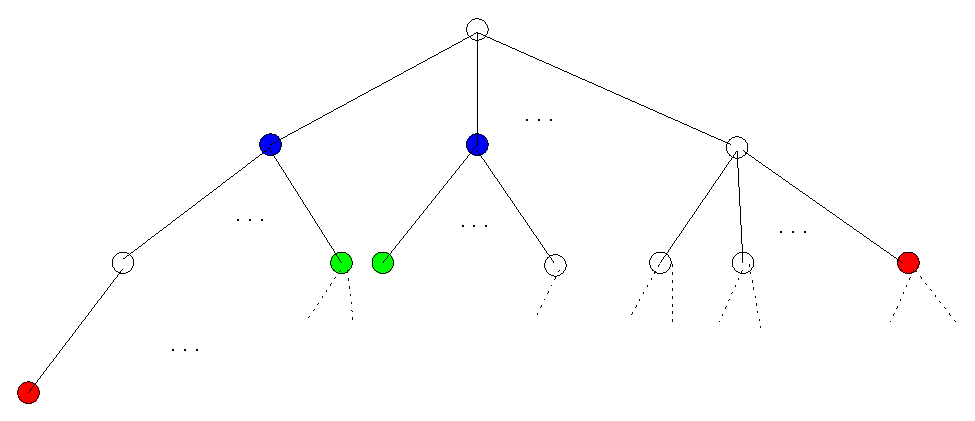
\includegraphics[width=0.7\textwidth]{tree}
  \caption{Graphical representation of a finitely branching tree; identically
    coloured nodes represent direct neighbors in the sense of $\prec_{1}$}
  \label{fig:finite-tree}
\end{figure}

The typical property of breadth-first search is that it `finds' the shallowest
node in the tree $r$ satisfying the property $p$, \IE in our case it assigns
this node to the reference $x$. Therefore, we impose an order $\prec_1$ on the
elements of the tree by defining a subtree $t_1$ to \emph{directly precede} a
subtree $t_2$ (written $t_1 \prec_1 t_2$) iff $t_1$ lies on the same level as $t_2$
does (with respect to a graphical representation similar to the one of Figure
\ref{fig:finite-tree}) and the former is its direct left-hand neighbor, or $t_1$
is the rightmost element in some level $n$ and $t_2$ is the leftmost element in
level $n+1$. By taking the transitive closure $\prec$ of $\prec_1$
\[
t \prec t' \quad\defeq \exists t_1\ldots t_n\bnd t \prec_1 t_1, t_1 \prec_1 t_2, \ldots,  t_n \prec_1 t'
\]
we obtain a means to say that a subtree $t$ \emph{precedes} some other subtree
$t'$. From these definitions, it is clear that 
\[t_1 \prec t_2 \land \lnot \exists t \in r.\; t_1\prec t\prec t_2 \quad\text{iff}\quad t_1 \prec_1 t_2\]
To put it formally, our goal will then be  to prove
\[
  (\exists t \in r\bnd p\ t) \Rightarrow [\ibox{bfs p r}](\rd{x} = \inr\, t_0 \land (p\ t_0) \land \forall t \in r\bnd p\ t \Rightarrow t = t_0 \lor t_0 \prec t)
\]
where, in the following we will be a bit sloppy about the value of $\rd{x}$ and
use $\rd{x}$ in place of the tree $t$ if $\rd{x} = \inr t$, and say $\rd{x} =
\unit$ if actually $\rd{x} = \inl \unit$. This will not lead to ambiguities,
since no tree is of the form $\unit$.
\begin{rem}
\label{rem-chld}
One has $t_1 \prec t_2 \Rightarrow \forall c_1\in\chld t_1, c_2 \in \chld t_2.\; c_1 \prec
c_2$, which is immediate from the definition of relation $\prec$. Also, for 
each tree $t$ where $\chld t = [c_1,\ldots, c_n]$ it is clear that
$c_i \prec_{1} c_{i+1} \text{ for } 1\leq i<n$.
\end{rem}

% inq and relq
In order to reason about the contents of the current queue, we need two
additional monadic predicates $relq : (A \to A \to \Omega) \to Q\ \Omega$ and $inq : A \to Q\ \Omega $
which intuitively state that a given relation holds for adjacent elements in the
queue, respectively that an element is contained in the queue. One could define
these predicates by means of the iteration construct $\op{iter}$ for which an
inference rule exists (see \cite{SchroederMossakowski:PDL}). In this case,
however, the definitions as well as the proofs involving them become quite
unwieldy. We therefore take another approach and axiomatise one further
deterministically side-effect free operation $\get$, which lets us
\emph{look inside} the queue by returning a list of all elements in the queue.
We will use notation $(x:xs)$ for a list with head $x$ and tail list $xs$ as
well as $(xs\uparrow x)$ for a list with endmost element $x$ and initial part $xs$.

\begin{flalign*}
& \mathbf{Axioms}\\
& \AssertDsef{get} && \text{(dsef-get)} \\
& (\get = xs) \Rightarrow  \PDLBox{\enq x}{(get = (xs\uparrow x))} && \text{(enq-app)} \\
& (\get = (x:xs)) \Rightarrow \PDLBox{y \leteq \deq}{(x = y \land \get = xs)} && \text{(deq-tl)} \\
& \qmt \iff (\get = []) && \text{empty-nil}
\end{flalign*}

An essential operation on queues we will need in our correctness proof is
$\op{last}$. With $\get$ available, this is just an abbreviation, assuming
there is a function $\op{lst}$ on lists that returns the last element in the list:

\[
(x = \last) \quad:\Leftrightarrow\quad x = (\op{lst}\ get)
\]

Obviously,
one has $(\get = xs\uparrow z) \Rightarrow (last = z)$.

\begin{defn}[$\relq$ and $\inq$]
\begin{eqnarray}
\label{eq:def-relq}
%\relq\, R &\defeq& \PDLBox{q\leteq\get}{(\forall i.\; 0\leq i<\op{len}\ q -1 \Rightarrow q^i R
%q^{i+1})} \\
\relq\, R &\defeq& \get = q \Rightarrow (\forall i.\; 0\leq i<\op{len}\ q -1 \Rightarrow q^i R q^{i+1}) \\
\label{eq:def-inq}
%\inq\, x &\defeq& \PDLBox{q \leteq \get}{(\exists i.\; 0\leq i<\op{len}\ q \land q^i = x)}
\inq\, x &\defeq& \get = q \Rightarrow (\exists i.\; 0\leq i<\op{len}\ q \land q^i = x)
\end{eqnarray}
Where $q^i$ denotes the $i$-th element of the list $q$, with the count
starting at zero.
\end{defn}

%% the loop invariant

The main problem, as often encountered in proofs involving a while-loop, is to
establish a loop invariant, \IE a condition that holds before the loop
and is re-established at each iteration of the loop. 
The first thing to remain invariant is the in-queue relation $\relq \prec_1$, as we will
see. This makes sure that all items in the tree are searched `in
order'. Furthermore, if $x$ has not been assigned a value, there are two
cases: either the queue is empty, in which case there is no element in the
tree satisfying $p$ (which would contradict the  assumptions), or the queue is not
empty and two conditions hold, abbreviated as follows:
\begin{eqnarray}
\label{eq:def-nf}
NF(t) &\defeq& \forall t'\in r.\; t' \prec t \Rightarrow \lnot p\, t' \\
\label{eq:def-cin}
CIN(t) &\defeq& \forall c\in r.\; \inq c \Leftrightarrow \exists t' \in r.\; c\in \chld t' \land t' \prec t \prec c
\end{eqnarray}
$[t \leteq \deq]NF(t)$ states that for all elements preceding $t$ property $p$ does
not hold, and $[t\leteq \deq]CIN(t)$ states that the elements in the queue are
exactly the children of elements $t'$  preceding $t$, whose children are
preceded by $t$. Now the case $\lnot (\rd{x}=\unit)$ must be considered, where it is said
that $p\, \rd{x}$ holds and all elements before $\rd{x}$ do not have property
$p$. Figure \ref{fig:inv} shows the whole formula.

\begin{figure}
\begin{center}
\fbox{
  \begin{minipage}{0.8\textwidth}
    \centering
    \[
    \begin{array}{clcll}
      & \ibox{relq}\; \prec_1 &&& \\
      \land & \rd{x} = \unit &\Rightarrow& \lnot \qmt \land {} & [t \leteq \deq](NF(t) \land CIN(t)) \\
      &        &  &\multicolumn{2}{l}{ \lor (\qmt \land \lnot \exists t \in r\bnd p\ t)} \\
      \land & \lnot(\rd{x} = \unit) &\Rightarrow&\multicolumn{2}{l}{p\, \rd{x} \land \forall t \in r\bnd p\ t \Rightarrow \rd{x} = t
      \lor \rd{x} \prec t} \\
    \end{array}
    \]
  \end{minipage}
}
\end{center}
\caption[A loop invariant]{Loop invariant $INV$ for the proposed breadth-first search}
\label{fig:inv}
\end{figure}

\subsection{Basic Facts}
Before providing the proof, we note some basic facts we will use later on.
\begin{lem}
In a non-empty queue, $\enqAll$ and $\deq$ may be swapped:
\label{enqAll-deq}
\begin{eqnarray*}
&& \lnot \qmt \land [\enqAll xs][t\leteq\deq]\varphi\;t \\
&\Leftrightarrow \quad& \lnot \qmt \land [t\leteq\deq][\enqAll xs]\varphi\;t
\end{eqnarray*}
\end{lem}

\begin{proof}
By induction on the structure of $xs$. In the base case, $xs = []$, by
(dsef$\Box$) we have $[\ret\unit]\varphi \Leftrightarrow \varphi$ and thus $[\enqAll xs]\varphi \Leftrightarrow \varphi$
by the definition of $\enqAll$. So the base case is trivially true.

In the inductive step, let $xs = (y: ys)$, so we need to show
\begin{eqnarray*}
&& \lnot \qmt \land [\enq y; \enqAll ys][t\leteq\deq]\varphi\;t \\
&\Leftrightarrow \quad& \lnot \qmt \land [t\leteq\deq][\enq y; \enqAll ys]\varphi\;t
\end{eqnarray*}
By the inductive hypothesis, the left-hand part of the formula can be
equivalently 
reformulated as $\lnot \qmt\land [\enq y][t\leteq\deq][\enqAll ys]\varphi\;t$ and then, by axiom
(swap) this is equivalent to the right-hand side of the formula
\end{proof}


\begin{lem}
\label{thm:enq-relq}
Under the stated conditions, we can add an element into the queue without
losing property $\relq R$:
\begin{eqnarray*}
\text{(i)} && \lnot \qmt \land \last\; R\;x \land \relq\; R \Rightarrow [\enq x]\relq\; R \\
\text{(ii)} && \qmt \Rightarrow [\enq x]\relq\; R
\end{eqnarray*}
\end{lem}

\begin{proof} 
  For (i), we reformulate $\lnot \qmt$ as $\get = xs\uparrow y$ (which indeed is an
  existential statement: there are some $xs$ and $y$ with this property), from
  which it follows that $\last\;R\;x$ is $yRx$ and $\relq\;R$ simplifies to 
  $\forall i\bnd 0\leq i<\op{len}\ xs \Rightarrow (xs\uparrow y)^iR(xs\uparrow y)^{i+1}$. The latter two formulas
  are stateless, such that together with axiom (get-app) one has
  \begin{equation}\begin{split}\nonumber
 \get = (xs\uparrow y) \land yRx \land \forall i\bnd 0\leq i<\op{len}\ xs \Rightarrow (xs\uparrow y)^iR(xs\uparrow y)^{i+1} \Rightarrow \\
  \PDLBox{\enq\ x}{\get = (xs\uparrow y\uparrow x) \land yRx \land \forall i\bnd 0\leq i<\op{len}\ xs \Rightarrow (xs\uparrow
    y)^iR(xs\uparrow y)^{i+1}}
  \end{split}
  \end{equation}
where the formula in the scope of the box operator implies $\relq\ R$, which finishes
  the proof by an application of rule (wk$\Box$).


  Concerning (ii), the conclusion is obvious from the premise and the definition
  of $\get$ and $\relq$.
\end{proof}


\begin{rem}
\label{rem:ext-enq-relq}
One can generalise Lemma \ref{thm:enq-relq} in the sense that it is also
possible to insert lists of items $[x_1,\ldots ,x_n]$ for all $n \in \mathbb{N}$ if
$x_i R x_{i+1}$ for $i \in \{1,\ldots,n-1 \}$ and $x_1$ may be enqueued without breaking
the relation $\relq\ R$.  The proof thereof proceeds by
structural induction on the to-be-inserted list.
\end{rem}

\begin{lem}
\label{thm:relq-deq}
If the relation $R$ holds in the queue, \IE $\relq\; R$, then after removing one
element, $R$ still holds: $\relq\; R \Rightarrow [x\leteq\deq]\relq\; R$. 
\end{lem}

\begin{proof}
For $\get = []$, the formula holds trivially, so assume $\get = (y: ys)$. From
the definition of $\relq$, we can deduce $\forall i.\; 0\leq i<len (y: ys) - 1 \Rightarrow
(y: ys)^iR(y: ys)^{(i+1)}$, so in particular $R$ holds for all adjacent
elements in $ys$. By (deq-tl) we obtain the desired result.
\end{proof}


\begin{lem}
\label{thm:enqAll-inq}
After inserting some elements $xs$ into the queue, for each $x\in xs$ we have
$\inq x$. Put formally:
\[
[\enqAll xs](\forall x\in xs\bnd \inq x) \quad \text{for all lists $xs$}
\]
\end{lem}
\begin{proof}
  Since $\get$ is dsef and thus always defined, we always have $\get = ys$ for
  some list $ys$. Now as usual we proceed by induction on the structure of $xs$ and
  leave out the base case, where $\enqAll$ does nothing and there are no
  elements to make a statement about. So let $xs = (x':xs')$.  It then follows
  by (get-app) that $[\enq x'](get = (ys \uparrow x'))$ and so $[\enq x'](\inq x')$. By
  the induction hypothesis we have
\[
[\enqAll xs'](\forall x\in xs'\bnd \inq x)
\]
and by application of (nec) we obtain
\[
[\enq x'][\enqAll xs'](\forall x\in xs'\bnd \inq x)
\]
The missing ingredient for finishing the proof is
\[
\inq x \Rightarrow [\enqAll xs]\inq x \quad \text{for all $x$ and $xs$}
\]
But this fact is again provable by induction on the mentioned $xs$ and follows
quite directly. Altogether we arrive at
\[
[\enq x'][\enqAll xs'](\forall x\in xs'\bnd \inq x \land \inq x')
\]
which actually is what we claimed, recalling that $(x':xs') = xs$
\end{proof}


%Actually, we do not have to axiomatise $\get$; it rather drops out of the
%previous axioms, if it is defined like follows.
%\begin{thm}
%\label{get-defn}
%Let
%\[
%\get\quad := (iter\; (\LambdaTerm{\Arg}{\lnot \qmt})\; (\LambdaTerm{z}{y \leteq \deq; ret (z\uparrow y)})\; [])
%\]
%In this case, the formulas \emph{enq-app}, \emph{deq-tl} and \emph{empty-nil}
%hold in a modified form accomodating the fact that $\get$, as defined here, is not dsef.

%XXX Not yet clear. No well-foundedness on the queue except empty, which we
%cannot say too much about.
%\end{thm}


%\begin{verbatim}
%deqAll :: Q a [a]
%deqAll = do if empty
%               then return []
%               else do x  <- deq
%                       xs <- deqAll
%                       return (x:xs)
%\end{verbatim}


%%%%%%%%%%%%%%%%%%%%
\begin{lem}
\label{deq-inq}
If the relation $\prec$ (or in fact any other strict partial order) holds in the
queue, then after removing an element $x$ from it, there is no element $y$ in
the queue with $x = y$
\[
\relq \prec \quad\Rightarrow\quad [x \leteq \deq](\lnot \inq x)
\]
\end{lem}

\begin{proof}
  We only need to consider the case where $\get = (y:ys)$. Assuming $\relq \prec$
  amounts to saying that
\[
\forall i.\; 0\leq i<len\ (y:ys) -1 \Rightarrow (y:ys)^i \prec (y:ys)^{i+1} \tag{$\star$}
\]
holds. By (deq-tl), after dequeuing only the $ys$ remain in the queue:
\[
\get = (y:ys) \Rightarrow [x \leteq \deq](\get = ys) \tag{$\star\star$}
\]
Noting that $\prec$ is a transitive and irreflexive relation (\IE $\forall x\,y\,z\bnd x
\prec y \land y \prec z \Rightarrow x \prec z$ and $\forall x \bnd x \not\prec x$) we may by $(\star)$ infer that there
is no $y'$ in $ys$ such that $y' = y$. But then, by $(\star\star)$, we are already done:
after dequeuing $x$, the $ys$ remain, in which there is no element equal to
$x$. 
\end{proof}

\begin{lem}
\label{inq-deq-eq}
Dequeuing an element does not affect existence of other elements inside the queue: 
\[
\inq x \Rightarrow [y \leteq \deq](x = y \lor \inq x)
\]
\end{lem}

\begin{proof}
  For $\get = []$, $\inq x$ is obviously false for every $x$.  For $\get =
  [x_1,\ldots,x_n]$, assuming $\inq x$ amounts to saying that there is an $x_i = x$
  for some $i,\; 1\leq i\leq n$. By (deq-tl) have $[y \leteq \deq](y = x_1 \land get =
  [x_2,\ldots,x_n]$ and thus for $x = x_1$ have $[y \leteq \deq](x = y)$ whereas for
  $x \neq x_1$ -- \IE $x = x_i$ for $1 < i \leq n$ -- have $[y \leteq \deq](\inq x)$,
  so altogether $[y \leteq \deq](x = y \lor \inq x)$ (cf. also Lemma
  \ref{thm:more-distrib}).
\end{proof}

\subsection{Auxiliary Rules}

In merging the specifications of the queue monad and the reference monad
(\cite{SchroederMossakowski:Hoare}), a typical frame-problem arises: The question \emph{`what
  remains the same in a changing world?'} can be instantiated here as \emph{`what
  happens to references if we modify the queue?'} The answer will certainly be
\emph{`nothing'}, which we formalise as follows.
\begin{equation}
\label{eq:frame1}
(x = \rd{r}) \Rightarrow [\mathbf{qop}](x = \rd{r}) \quad\text{for }\mathbf{qop} \in \{\deq, \enq, \qmt \} 
\end{equation}
The simplest way to answer the converse question \emph{`what happens to the queue
if we modify a reference?'}  is by relating $\get$ to reference writing:
\begin{equation}
\label{eq:frame2}
(\get = xs) \Rightarrow [r := x](\get = xs)
\end{equation}
Reference to one of these axioms will be indicated by (frame).

In \cite{SchroederMossakowski:PDL} a Hoare calculus for total correctness has been
developed, in which Hoare rules such as
\[
\text{\bf (seq)}\quad
\begin{array}{@{}c@{}}
[\varphi]\overline{x} \leteq \overline{p}[\psi] \\
{}[\psi]\overline{y} \leteq \overline{q}[\chi] \\\hline
{}[\varphi]\overline{x} \leteq \overline{p}; \overline{y} \leteq \overline{q}[\chi]
\end{array}
\]
appear. It has been said in Section \ref{sec:hoare-calculi} that a Hoare rule
$[\varphi]\overline{x} \leteq \overline{p}[\psi]$ is meant to be interpreted as $\varphi \Rightarrow
(\langle\overline{x} \leteq \overline{p}\rangle\top \land [\overline{x} \leteq \overline{p}]\psi)$. In
this way, partial correctness as well as termination of a program sequence
$\overline{p}$ and thus total correctness are concisely captured.

Because we are working with formulas of dynamic logic and do not want to switch
into the Hoare calculus, yet we would like to use the results of the latter, we
simply translate some Hoare rules of \cite{SchroederMossakowski:PDL} 
back into rules for dynamic logic.

\begin{eqnarray*}
\NRule{dsef1}{\text{p dsef}}{\varphi \Rightarrow [p]\varphi}
\qquad
\NRule{if}{\begin{array}{@{}c@{}}
             \text{b dsef}\\
             \varphi \land b \Rightarrow [x \leteq p]\psi\\
             \varphi \land \lnot b \Rightarrow [x \leteq q]\psi
           \end{array}}
           {\varphi \Rightarrow [x \leteq \IfTerm{b}{p}{q}]\psi}
\\
% \\
% \text{\bf (dsef2)}\quad
% \frac{\text{p dsef}}{[x \leteq p](x = p)}
% \qquad
% 
% \qquad
% \text{\bf (seq)}\quad
% \begin{array}{@{}c@{}}
% \varphi \Rightarrow [\overline{x} \leteq \overline{p}]\psi \\
% {}\psi \Rightarrow [\overline{y} \leteq \overline{q}]\chi \\\hline
% {}\varphi \Rightarrow [\overline{x} \leteq \overline{p}; \overline{y} \leteq \overline{q}]\chi
% \end{array}
\NRule{while}{\begin{array}{@{}c@{}}
                t : DB\\
                \Arg < \Arg : B \times B \to \Omega \text{ is well-founded}\\
                \varphi \land b \Rightarrow \PDLDmd{p}{\top}\\
                (\varphi \land b \land t =_B z) \Rightarrow [p](\varphi \land t < z) \end{array}}
     {\varphi \Rightarrow \PDLBox{\WhileTerm{b}{p}}{(\varphi \land \lnot b)} \land \PDLDmd{\WhileTerm{b}{p}}{\top}}
\end{eqnarray*}

In rule (while) termination is ensured by letting the term $t$ decrease strictly
in every iteration. Since $<$ is well-founded, it is impossible for the final
premiss to be true infinitely often. The so called \emph{ghost variable} $z : B$
does not appear within the program and simply serves the purpose of relating the
value of $t$ before and after execution of $p$. In particular, $t$ is not equal
to $z$ as a computation, but rather its value equals $z$.

Now we are equipped with all we
need to prove total correctness of the program $\op{bfs}$, in particular -- as
can be seen from the rule for while -- termination of the while-loop.

%%%%%%%%%%%%%%%%%%%%%%%%%%%%%%%%%%%%%%%%%%%%%%%%%%
% The proof
\subsection{Proof of Total Correctness}

In what follows, we try not to be too formalistic and therefore make reference
to common laws such as transitivity of equivalence or other obvious validities
without proving them for each separate instance.  We further assume that the
underlying formalism is classical, \IE we allow reasoning by case distinction
over some formula $\phi \lor \lnot \phi$. In a Hilbert-style calculus with essentially only
modus ponens availabe as an inference rule, methods such as proof by
contradiction are to be conceived as first proving $\lnot P \Rightarrow \False$ and then
applying (mp) to the tautologous $(\lnot P \Rightarrow \False) \Rightarrow P$. Likewise, substitutivity
of equivalence makes use of the tautology scheme $(P \Leftrightarrow Q) \Rightarrow R[P/x] \Rightarrow R[Q/x]$.

It will now first be established that $INV$, the loop invariant, holds before the while
loop, \IE with $PRE \defeq \exists t \in r\bnd p\ t$ (a stateless formula) we show 
\begin{equation}
\label{eq:est-inv}
PRE \land \qmt \Rightarrow [x := \unit ; \enq r](INV)
\end{equation}

\begin{subequations}
By (read-write) and (frame)
\begin{equation}
\label{eq:est01}
[x := \unit; \enq r](\rd{x} = \unit) 
\end{equation}
From the definition of $\relq$ we can infer
\begin{equation}
\qmt \Rightarrow [\enq r](\relq \prec)
\end{equation}
which by (frame) can be extended to
\begin{equation}
\label{eq:est02}
\qmt \Rightarrow [x := \unit; \enq r](\relq \prec) 
\end{equation}
Again with (frame), (enq-deq) gives us
\begin{equation}
\label{eq:est03}
\qmt \Rightarrow [x:= \unit; \enq r][t \leteq deq](r = t \land \qmt)
\end{equation}
\end{subequations}

Now from $r = t$ we can deduce $NF(t)$, because there simply is no element $t' \prec
r$ in $r$. Similarly, we infer $CIN(t)$ because $\inq c$ is false for every
element in $r$ and again there is no element $t' \prec r$, so the equivalence in
$CIN$ holds.  Combining (\ref{eq:est01}), (\ref{eq:est02}) and (\ref{eq:est03})
we obtain the desired result.

\paragraph{The while rule}
The next step is to gather the premisses of the (while) rule as stated above to
draw the conclusion of selfsame. The premiss $INV \land \rd{x} = \unit \land \lnot \qmt \Rightarrow
\PDLDmd{\op{body}}{\top}$ asserting termination of the loop body $\op{body}$ is
quite obvious, since the only source of nontermination is the $\deq$-operation,
which will however only be executed if the queue is not empty. The formalisation
of this argument can be conducted along the lines of the following proof of the
most integral part:
\begin{equation}
\label{eq:prem-while}
\begin{array}{l}
INV \land \rd{x} = \unit \land \lnot \qmt \land vol = z \Rightarrow \\
 \qquad 
   [t \leteq \deq; \mathrm{if}\; p\ t\; \mathrm{then}\; x := inl\ t \;
   \mathrm{else}\; \enqAll \chld
t](INV \land vol < z)
\end{array}
\end{equation}
where we introduce the termination measure $vol$ which computes the total number
of elements reachable from any subtree contained in the queue. Employing the
list functions $\op{sum : [Nat] \to Nat}$ and $\op{map} : (A \to B) \to [A] \to [B]$ --
whose definitions are straightforward and can be found, \EG, in the Haskell
Prelude -- it might be defined like this:
\begin{alltt}
vol :: Q Nat
vol = do \{ q <- get; 
           ret sum (map volume q) 
         \}
    where volume :: Tree A -> Nat
          volume t = 1 + sum (map volume (chld t))
\end{alltt}
The intuition behind this approach is that the overall volume of the queue must
strictly decrease after dequeuing some subtree $t$ and enqueuing its children,
because the volume of $t$ is defined to be by 1 larger than the sum of volumes
of its children. $\op{vol}$ is a dsef operation since it is composed solely of
dsef operations (it has been shown in \Isabelle that dsef programs are stable
under composition).

% tomorrow never dies
We note the following equivalence which we shall use for simplification purposes
and whose right-hand part we will denote by $SI$.
\begin{eqnarray}
\label{eq:inv-equiv}
&& INV \land \rd{x} = \unit \land \lnot \qmt \\
&\Leftrightarrow& {\relq \prec_1} \land \lnot \qmt \land [t \leteq \deq](NF(t) \land CIN(t)) \land \rd{x} = \unit 
\nonumber
\end{eqnarray}

By Lemma \ref{thm:relq-deq} we have
\[
SI \Rightarrow [t \leteq \deq](\relq {\prec}_1)
\]
so by (frame) $\relq$ still holds after assignment to $x$:
\begin{equation}
\label{eq:then-part1}
SI \Rightarrow [t \leteq \deq][x := t](\relq {\prec}_1)
\end{equation}

\paragraph{Then-branch} 
Working our way through the
then-branch of the loop body, we also need the next statement. This is
obtained from (read-write) and the fact that $NF$ and $p\; t$ are stateless.
\begin{equation}
\label{eq:then-part2}
NF(t) \land p\;t \Rightarrow [x := t](\rd{x} = t \land p\;\rd{x} \land NF(t))
\end{equation}
Now, $NF(t) \land p\;\rd{x} \land \rd{x} = t$, \IE that all elements in the tree smaller
than $t$ do not have property $p$, but $t$ and therefore $\rd{x}$ does, can be
reformulated as $p\;\rd{x} \land \forall t\in r\bnd p\;t \Rightarrow \rd{x} = t \lor \rd{x} \prec t$. 
% Regarding
% the decrease in volume, one has $\lnot \qmt \Leftrightarrow get = (x:xs)$ for some list $(x:xs)$
% and thus 
% \begin{equation}
% SI \land get = (x:xs) \land vol = z \Rightarrow [x:= t]
% \end{equation}


In combining
\eqref{eq:then-part1} and \eqref{eq:then-part2} we obtain the following, where
the formula in the scope of the  $[x := t]$ box is in fact stronger than $INV$
\begin{equation}
\label{eq:prem-then}
\begin{array}{l@{\quad}l}
& \relq {\prec}_1 \land NF(t) \land p\;t \\
 \Rightarrow& 
   [x := t](\rd{x} = t \land p\;\rd{x} \land \relq {\prec}_1\\
&\qquad {} \land (\forall t'\in r\bnd p\;t\Rightarrow\rd{x} = t' \lor \rd{x} \prec t')
\end{array}
\end{equation}

\paragraph{Else-branch}
Because all ingredients needed for the then-part are now assembled, we turn our
eyes to the else-part, which actually is the harder one. `Inside' the $[t \leteq
\deq]$ box of \eqref{eq:prem-while}
we have $CIN(t) \land NF(t) \land relq {\prec}_1 \land \rd{x} =  \unit$. We will, in accordance with the if-rule,
furthermore assume $\lnot p\;t$ and prove the following, in which again the formula
inside the $[\enqAll (\chld t)]$ box implies $INV$
\begin{equation}
\label{eq:prem-else}
\begin{array}{l@{\quad}l}
&  CIN(t) \land NF(t) \land \relq {\prec}_1 \land \lnot p\;t \land \rd{x} =  \unit \\
\Rightarrow & [\enqAll (\chld t)](\relq {\prec}_1 \land \rd{x} =  \unit   \\
&  \quad {}\land (\lnot \qmt \land [t' \leteq \deq](NF(t') \land CIN(t')) \\
& \qquad  {}\lor (\qmt \land \lnot \exists t''\in r\bnd p\;t'')))
\end{array}
\end{equation}
This can by Lemma \ref{thm:box-and-distrib} be done in three steps, each asserting
the truth of the above formula reduced to one of the three conjunct clauses in
the scope of the enqAll box.

\paragraph{part i}
\[
% CIN(t) \land NF(t) \land \relq {\prec}_1 \land \lnot p\;t \land 
\rd{x} = \unit \quad \Rightarrow 
\quad [\enqAll (\chld t)]\;(\rd{x} =  \unit )
\]
Now this is an obvious generalisation of one of the frame axioms.

\paragraph{part ii}
\begin{eqnarray*}
  && CIN(t) \land NF(t) \land \relq {\prec}_1 \land \lnot p\;t \land \rd{x} = 
  \unit \\
  &\Rightarrow& [\enqAll (\chld t)]\,(\relq {\prec}_1)
\end{eqnarray*}
This formula asserts that we may enqueue $t$'s children without destroying the
relation $\relq \prec_1$ inside the queue. For $\chld\ t = []$ we must then prove $\ldots
\land \relq{\prec}_1 \Rightarrow \PDLBox{\ret\unit}{\relq{\prec}_1}$, which essentially is given by
(ret$\Box$). So let $\chld\ t = (x:xs)$.  Then by Remark \ref{rem:ext-enq-relq} all
children may be inserted through $\enqAll$ without invalidating $\relq {\prec}_1$ if
$x$ may be enqueued through $\enq$. For $\qmt$ this is clearly true, so
consequently we'll add the premiss $\lnot \qmt$. Then $CIN(t)$ tells us $\inq c$
holds for exactly all the child elements $c$ of predecessors of $t$. Thus $\last
\prec x$ certainly holds (cf. Remark \ref{rem-chld}). Because $\lnot \exists a\in r\bnd \last \prec
a \prec x$, even $\last \prec_1 x$ is true, providing all the premisses of Lemma
\ref{thm:enq-relq} and letting us draw the desired conclusion. $\lnot \exists a\in r\bnd
\last \prec a \prec x$ can be shown by contradiction: assume $\exists a\in r\bnd \last \prec a \prec x$;
Then it directly follows that there is $t''$ such that $a \in \chld t''$ and $t''
\prec t$ ($t'' = t$ cannot be the case since $a \prec x$, and for the same reason $t \prec
t''$ neither). But then, because of $CIN(t)$, $\inq a$ holds, which together
with $\last \prec a$ violates the given premiss $\relq {\prec}_1$. We conclude that
part ii is true.

\paragraph{part iii}
\begin{eqnarray*}
&& CIN(t) \land NF(t) \land \relq {\prec}_1 \land \lnot p\;t \land \rd{x} =  \unit\\
&\Rightarrow& [\enqAll (\chld t)]\,(\lnot \qmt \land [t' \leteq \deq](NF(t') \land CIN(t')) \\
&& \qquad  {}\lor (\qmt \land \lnot \exists t''\in r\bnd p\;t''))
\end{eqnarray*}
This part makes sure that after inserting $t$'s child elements we either have seen
each element in the tree and none satisfies $p$, or there are elements left and
after dequeuing another element $t'$ all its predecessors don't have property
$p$ and the elements remaining in the queue are exactly the children of
predecessors of $t'$, which themselves are succeeding $t'$.

We proceed by case distinction over $\qmt \lor\lnot \qmt$. We have 
\[ \qmt \Rightarrow [\enqAll (\chld t)]\;\qmt \quad\text{iff}\quad \chld t = []
\]
 But in this case, \IE when $\qmt$ holds in the box, $t$
must be the final element in the tree $r$ since all children of predecessors
would otherwise be in the queue (by $CIN$). Extend $NF(t)$ and $\lnot p\;t$ to $\lnot \exists
t''\in r\bnd p\;t''$ and obtain $[\enqAll (\chld t)](\qmt \land \lnot \exists t''\in r\bnd
p\;t'')$ making the conclusion of part iii true. For $\chld t = (x:xs)$
one has $\qmt \Rightarrow [\enqAll (\chld t)](\lnot \qmt)$. Here, $t \prec_1 x$ must hold, \IE
t's first child element is its direct successor, because no element before $t$
has child elements that are in the queue by $CIN(t) \land \qmt$.  Now
\[
[\enq x; \enqAll xs][t' \leteq \deq](NF(t') \land CIN(t')))
\]
is by Lemma \ref{enqAll-deq} equivalent to 
\[
[\enq x; t' \leteq \deq][\enqAll xs](NF(t') \land CIN(t'))
\]
and because of (enq-deq) one has:
\[
\qmt \Rightarrow [\enq x; t' \leteq \deq; \enqAll\ xs](x = t')
\]
So it suffices to prove the implication
\[ 
\ldots \Rightarrow [\enq x; t'\leteq\deq][\enqAll xs](CIN(t') \land NF(t'))
\]
where $\ldots$ denotes the premisses $\lnot p\,t$, $t {\prec}_1 x$, $CIN(t)$, $NF(t)$ and
$\qmt$.

The $NF$ part is fairly easy to see: one certainly has $NF(t) \land t {\prec}_1 t' \land \lnot
p\,t$ inside the box, which implies $NF(t')$, where $t'$ replaced $x$ due to
their being equal.  $CIN(t')$, which decodes into $CIN(t') \defeq
\forall c\in r.\; \inq c \Leftrightarrow \exists t'' \in r.\; c\in \chld t'' \land t'' \prec t' \prec c$, is true due to the
fact that exactly the $xs$ are in the queue, and for each $x' \in xs$ we have $x'
{\prec} x$. That finishes the case where $\qmt$ is true.

Now for the case where $\lnot \qmt$ is taken as a premiss and -- to restate the
other ones -- $CIN(t)$, $NF(t)$, $\relq \prec_1$ and $\lnot p\,t$. Obviously one then has
$\ldots \Rightarrow [\enqAll (\chld t)](\lnot \qmt)$, so it remains to be proven that
\[
\ldots \Rightarrow [\enqAll (\chld t)][t' \leteq \deq](NF(t') \land CIN(t'))
\]
or, equivalently and quite similar to the case above we can show
\[
\ldots \Rightarrow [t' \leteq \deq][\enqAll (\chld t)](NF(t') \land CIN(t'))
\]
For $NF(t')$ alone, this can be done if $\ldots \Rightarrow [t' \leteq \deq](t {\prec}_1 t')$ can be shown,
because unlike $CIN(t')$, $NF(t')$ is indeed a stateless formula about a
property of the tree $r$ and not about the monadic queue. Hence $NF(t') \Rightarrow
[\enqAll (\chld t)](NF(t'))$ by (K3$\Box$). For
the same reason, however, $NF(t)$ holds after execution of $\deq$: $NF(t) \Rightarrow [t'
\leteq \deq](NF(t))$ so that at least for $NF(t')$ the proof goes through: we have
\begin{equation}
\label{eq:deq-nf}
\ldots \Rightarrow [t' \leteq \deq](NF(t) \land t {\prec}_1 t')
\end{equation}
because the direct successor of $t$ must be in the queue, asserted by $CIN(t)$
together with $\lnot\qmt$, and it must be `the next one to drop out of it', given
by $\relq {\prec}_1$. From this and $\lnot p\,t$ we infer
\[
[t' \leteq \deq](NF(t'))
\]
And then by the argument given above
\[
\ldots \Rightarrow [t' \leteq \deq][\enqAll (\chld t)](NF(t'))
\]

Continuing with the premisses $\lnot \qmt$ and $CIN(t) \land NF(t)$, $\relq \prec_1$ and $\lnot
p\,t$ we will now show the final piece of the puzzle, viz. that these imply
\begin{equation}
% \tag{hans}
\label{peter}
[t' \leteq \deq][\enqAll (\chld t)](CIN(t'))
\end{equation}

We proceed as follows; let $\get = [x_1,\ldots,x_n],\; n \geq 1$.  By Lemma
\ref{deq-inq} and fact \eqref{eq:deq-nf} we have
\[
\ldots \Rightarrow [t' \leteq \deq](\lnot \inq t' \land get = [x_2,\ldots, x_n] \land t {\prec}_1 t' \land t' = x_1)
\]
$CIN(t)$ tells us that the $x_i\; (1\leq i\leq n)$ are exactly those elements for which
$x_i \in \chld t_i \land t_i \prec t \prec x_i$ is true for appropriate $t_i$. With $t \prec_1 t'$
it is clear that all elements $c$ satisfying $c \in \chld t_i \land t_i \prec t' \prec c$ for
appropriate $t_i$ are $x_2,\ldots,x_n$ (a possibly empty sequence) plus the child
elements of $t$ (pointing out that $t'$ cannot be a child of $t$ because
$t' = x_1$ and therefore is a child of some predecessor of $t$ by $CIN(t)$). With
$\chld t = [c_1,\ldots,c_k]$ one has by structural induction
\[
\get = [x_1,\ldots,x_n] \Rightarrow [t' \leteq \deq][\enqAll (\chld t)](get = ((\ldots([x_2,\ldots,x_n]\uparrow c_1)\uparrow \ldots ) \uparrow c_k))
\]
or slightly more readable
\[
[t' \leteq \deq][\enqAll (\chld t)](get = [x_2,\ldots,x_n,c_1,\ldots,c_k])
\]
from which we conclude by the foregoing argument that for the given premisses we
can show
\[
\ldots \Rightarrow [t' \leteq \deq][\enqAll (\chld t)](CIN(t'))
\]

\subsubsection{Assembling the Results}

We may finally apply rule (if) to formulae \eqref{eq:prem-then} and
\eqref{eq:prem-else} repeating that in both ones, the subformulae inside the
boxes imply $INV$
\begin{equation}
\label{eq:concl-if}
\begin{array}{l@{\quad}l}
&  CIN(t) \land NF(t) \land \relq {\prec}_1 \land \rd{x} =  \unit \\
\Rightarrow & \PDLBox{\IfTerm{p\ t}{x:=t}{\enqAll (\chld\ t)}}(INV)
\end{array}
\end{equation}
Referring to \eqref{eq:inv-equiv}, we can say
\begin{equation}
\label{eq:si-deq}
SI \Rightarrow [t \leteq \deq](CIN(t) \land NF(t) \land \relq {\prec}_1 \land \rd{x} =  \unit )
\end{equation}

Regarding the decrease in volume, which has silently been passed over until now,
one has $\lnot \qmt \Leftrightarrow get = [x_1,\ldots,x_n]$ for some elements $x_i$ and some $n$ and
thus by (deq-tl) and the definition of $\op{vol}$ resp. $\op{volume}$
\begin{eqnarray}
\label{eq:then-vol}
&& \op{volume} x > 0 \nonumber \\
&& SI \land \get = [x_1,\ldots,x_n] \land vol = z \nonumber \\ {}
& \Rightarrow &[t \leteq \deq](get = [x_2,\ldots,x_n] \land vol = (z - \op{volume} x_1))
    \nonumber \\
&& \text{so by (frame)} \nonumber\\
& & SI \land get = [x_1,\ldots,x_n] \land vol = z \\
&\Rightarrow& [t \leteq \deq; x:= t](vol < z) \nonumber
\end{eqnarray}
Now in addition let $\chld t = [c_1,\ldots,c_k]$ such that after enqueuing these one
still has a smaller volume than before dequeuing $t$, since $t$'s volume is
defined to be by one larger than the sum of volumes of its child elements:
\begin{equation}
\label{eq:else-vol}
\begin{array}{ll}
& \op{volume} t = 1 + \sum_{i=1}^{k}(\op{volume} c_i)\\
& SI \land get = [x_1,\ldots,x_n] \land vol = z \\
\Rightarrow & [t \leteq \deq; \enqAll (\chld t)](get = [x_2,\ldots,x_n,c_1,\ldots,c_k] \land vol < z)
\end{array}
\end{equation}

Having ascertained the termination of the loop by \eqref{eq:then-vol},
\eqref{eq:else-vol}, we apply rule (wk$\Box$) to \eqref{eq:concl-if},
\eqref{eq:si-deq} to finally verify the premisses of rule (while) (cf.
\eqref{eq:prem-while}) and thus conclude
\begin{eqnarray*}
INV \Rightarrow [\WhileTerm{cond}{prog}](INV \land (x \neq \unit \lor \qmt)) \\
\begin{array}{ll@{\quad = \quad}l}
\text{where} & \op{cond} & x =  \unit \land \lnot \qmt \\
  &            \op{prog} & t \leteq \deq; \IfTerm{p\;t}{x:=t}{\enqAll (\chld\ t)}
\end{array}
\end{eqnarray*}

The definitely last step is now to derive the postcondition 
\[
(p\  \rd{x} \land \forall t \in r. p\ t \Rightarrow \rd{x} =  t \lor \rd{x} \prec t)
\]
from what the while loop left us with:
\[
(INV \land (x \neq \unit \lor \qmt)) 
\]
but this can be done easily, recalling that the stateless formula warranting
existence of an element satisfying $p$ still holds after execution of $\op{bfs}$
\[
(\exists t \in r\bnd p\ t) \Rightarrow [\op{bfs}\,p\, r](\exists t \in r\bnd p\ t)
\]
{\hfill \qed}


%%% Local Variables: 
%%% mode: latex
%%% TeX-master: "main"
%%% End: 



\chapter{The Theorem Prover Isabelle}
\label{cha:isabelle}

\Isabelle is an interactive theorem proving environment, \IE an assistant for
performing formal proofs. The fact that \Isabelle is generic in the sense that
it allows one to define and reason within several kinds of logics distinguishes
it from most other proof assistants. Examples of logics that have been defined
within \Isabelle's framework are classical first-order logic (FOL), constructive
type theory (CTT), or higher-order logic (HOL) which constitutes
the base logic in our development of monadic dynamic logic.

We will now introduce the foundations of \Isabelle which are the so called
meta-logic, its syntax and inference rules. We then introduce higher-order logic
as formalised in \Isabelle. Finally, we provide insight into basic proof methods
whose knowledge is necessary to comprehend or at least read printed \Isabelle
proofs. A full account of all facilities that were applied cannot be given in
this thesis; very readable introductions to \Isabelle and \IsabelleIsar can be
found in \cite{Nipkow03,IsabelleHOL}

But first, a note about terminology and the development of \Isabelle is in
order: Initially, communicating with \Isabelle meant sequentially applying ML
functions, since \Isabelle is written in this functional language. This user
interface has recently been discharged in favour of an independent proof and
theory language called \emph{Isar}, making proofs substantially more readable
(and maintainable). The combination of \Isabelle with Isar is named
\IsabelleIsar, which becomes Isabelle/Isar/HOL when referring to the
specific logic HOL, expressed in Isar. In the following, we will often use the
term \Isabelle for all these phrases, stating once and for all that the formal
proofs in this thesis are presented in \IsabelleIsar with HOL as the underlying
logic.


\section{The Meta-logic}
\label{sec:meta-logic}

\Isabelle lets the user define his own logics, so that he does not have to work
within a fixed logic that might not suit his needs. In doing so, one needs some
means to express the syntax of one's newly defined logic, to express inference
rules, and to impose side conditions on these rules. Take the following natural
deduction rule governing the introduction of the $\forall$-quantifier as an
example: 
\begin{equation}
  \Rule{P(x)}{\forall x.\,P(x)} \quad \text{($x$ not free in assumptions)}
\end{equation}
The annotation `$x$ not free in $\ldots$' is a very typical side condition,
while the horizontal bar expresses a possible logical inference from the
premisses (displayed above the bar) to the conclusion (below the bar).

Besides determining the basic syntax of all definable logics, it is the task of
the \emph{meta-logic} to enable the formulation of such `meta-logical'
constructs, \IE to formalise properties of concrete object-logics. Put shortly,
the meta-logic is an intuitionistic higher-order logic with polymorphic
functions in the style of ML or Haskell that possesses a universal quantifier,
implication and equality as its constants.


\subsection{Basic Syntax and Terminology}
\label{sec:meta-basic-syntax}

The meta-logic is syntactically based on the simply typed lambda calculus as
described in Section \ref{sec:adding-types} (although without product types).
The additional possibility to define polymorphic functions means that function
types may contain \emph{type variables}, \EG the identity function $\Id
\Map{\alpha}{\alpha}$ exists for \emph{every} type $\alpha$.  \emph{Type declarations} allow
the introduction of new base types, whereas \emph{type classes} may be seen as
collections of types that share some structure (a well-known example is the
class $\Type{ord}$, which the types with a notion of order among their elements
belong to). The latter concept comes close to Haskell's type classes, but is not
powerful enough to embrace Haskell's constructor classes as well. In particular,
the notion of a type constructor being an instance of a monad cannot be
specified in \Isabelle. A remark about how this problem has been resolved in the
implementation can be found in Section~\ref{sec:monads-isabelle}.

Some peculiarities of \Isabelle's syntax should be noted before proceeding: 
\begin{itemize}
\item The base type of truth values is named $\Type{prop}$.
\item Type annotations are denoted by two successive colons instead of one.
\item Function types may be built from existing types by means of the function
  type constructor $\Rightarrow$, such that $f \IsaMap{\sigma}{\tau}$ is \Isabelle's notation for
  $f\Map{\sigma}{\tau}$. The type constructor $\Rightarrow$ associates to the right.
\item The types of curried functions taking $n$ arguments, $f :: \sigma_1 \Rightarrow \cdots \Rightarrow \sigma_n \Rightarrow
  \sigma$ may be written in a list-like notation $f :: [\sigma_1,\ldots,\sigma_n] \Rightarrow \sigma$.
\item Type variables are written as Latin letters prefixed with an apostrophe
  ($'$), \EG $\ivar{a}$, $\ivar{b}$, $\ivar{b_1}$ are type variables. Inside
  normal text we will however not use this style.
\end{itemize}

The constants of the meta-logic are a universal quantifier, (denoted by the
symbol $\bigwedge$), implication ($\Longrightarrow$\footnote{note the difference between this symbol
  and the shorter one for the function type constructor $\Rightarrow$; both however
  associate to the right and there also is a list-like notation for repeated
  implication of the form $\llbracket\phi_1;\ldots;\phi_n\rrbracket \Longrightarrow \psi$}) and equality ($\equiv$). An interesting
property of higher-order logics that spring from the lambda calculus is the fact
that no variable binders other than $\lambda$ are needed: predicates are simply
interpreted as functions into truth values (\EG a predicate on the type
$\Type{nat}$ of natural numbers might be expressed as a function $P
\Map{\Type{nat}}{\Type{prop}}$), and quantifiers are interpreted as higher-order
functions from predicates to truth values. Thus, the type of the universal
quantifier is
\begin{equation}
  \label{eq:univ-quant-type}
  \bigwedge\nolimits_\alpha \IsaMap{(\alpha \Rightarrow \Type{prop})}{\Type{prop}}
\end{equation}
for each type $\alpha$; the polymorphism of \Isabelle is restricted in the same way
as in ML or Haskell in that it does not allow higher-order functions to take
polymorphic functions as arguments. This is made explicit here by indexing the
quantifier with the appropriate type under consideration.


\subsection{Defining Logics}
\label{sec:defining-logics}

Users are not expected to work within the meta-logic itself, but rather to
formalise their own logics by extending the meta-logic through the introduction
of new types and constants and through axioms capturing the properties of these
constants. An example is given in Section \ref{sec:higher-order-logic}, where
the formalisation of HOL within the meta-logic is described. The outline of such
a formalisation is as follows:
\begin{enumerate}
\item Introduce a new type for truth values, thereby distinguishing it from the
  type of truth values of the meta-logic. Furthermore introduce a predicate
  $\Fun{Trueprop}$ converting from object-level truth to meta-level truth; it
  has proved sensible to keep these two kinds of truth values apart. Other
  useful types may be added as well, of course.
\item Name and assign types to the constants that will serve as basic functions
  of the logic to be defined; examples include propositional connectives $\land$,
  $\longrightarrow$, etc., or even modal operators. It is possible to decorate constants with
  concrete syntax (by so called \emph{mixfix annotations}, cf. \cite{IsaRef04})
  that makes operations more readable than is possible with the minimalistic
  syntax of the lambda calculus. One way or the other, functions of the
  respective object-logic conventionally have higher precedence than those of
  the meta-logic.
\item Extend the meta-logic by further axioms that capture the properties of
  these constants and types. The basic idea is that axioms of the meta-logic are to be
  interpreted as rules in the object logic. For example, the typical
  rules for conjunction introduction and universal generalisation in first-order
  logic 
  \[ \Rule{P\quad Q}{P \land Q}\qquad \Rule{P\, x}{\forall x\bdot P\, x}\;\text{($x$ not
    free in assumptions)}\]
  might be formalised as 
  \[ \llbracket P; Q\rrbracket \Longrightarrow P \land Q\quad\text{and}\quad (\bigwedge x\bdot P\, x) \Longrightarrow \forall x\bdot P\, x \]
\end{enumerate}
Proofs from rules within the object-logic are then basically proofs from
corresponding axioms within the meta-logic.


\subsection{Meta-logic Rules}
\label{sec:meta-logic-rules}

To perform such proofs inside the meta-logic, a collection of meta-rules is
necessary. These rules are hard-wired into \Isabelle, which means they are
implemented as ML functions operating on meta-logic terms rather than being
terms of the meta-logic itself. A complete exposition of these rules
can be found in \cite[Section 2.4]{Paulson89}, which we do not repeat here,
since the meta-rules are virtually never applied in proofs inside object-logics.
Instead, we merely summarise the rules, giving an idea of the relative
compactness of the meta-logic. 

The meta-rules can roughly be put into three
categories:
\begin{enumerate}
\item Introduction and elimination rules for the constants $\bigwedge$, $\Longrightarrow$
and $\equiv$; 
\item Rules concerning lambda terms; put concretely, there is a rule for
$\alpha$-conversion, a rule for $\beta$-reduction admitting the conclusion $a[b/x]$ from
the premiss $(\LambdaTerm{x}{a})\ b$, and a rule of extensionality; 
\item  Finally,
there are basic rules for equality.
\end{enumerate}

\section{Higher-order Logic (HOL)}
\label{sec:higher-order-logic}

In this section we introduce the formalisation of the simply typed higher-order
logic HOL. The outstanding feature of higher-order logics is their
capability of expressing higher-order functions (in a sense similar to that of
functional programming languages), but also of expressing predicates and
quantification on arbitrarily typed terms. For example, one may state the
property of a set $S$ being infinite by expressing that there is an injective
function from $S$ into a proper subset $S' \subset S$:
\[
S\;\mathit{infinite} \quad\text{iff}\quad \exists S'\bnd S' \subset S\land\exists f :: S \Rightarrow S'\bnd f\
\mathit{injective}
\]
Because of the quantification on the function $f$ this statement is inherently
higher-order; it cannot even be expressed equivalently in first-order languages.
In HOL all functions are required to
be total; an extension incorporating concepts from domain theory that allows the
formulation of arbitrary computable functions is HOLCF
\cite{MuellerNipkowOheimbSlotosch}.  For in-depth descriptions of higher-order
logic and its implementation in \Isabelle, see \cite{Andrews00,IsabelleHOL}.


\subsection{Constants}
\label{sec:hol-constants}

HOL as implemented in \Isabelle extends the meta-logic by a number of constants
that are to be interpreted as the usual logical connectives, like conjunction,
universal quantification, or boolean case distinction (the familiar
\emph{if-then-else} construct). Differing from the notation used so far,
implication is denoted by a simple long arrow $\longrightarrow$. Some of the operations come
in two flavours, namely their functional form (as actual constants in the lambda
calculus of the meta-logic) and with some syntactical sugaring; Table
\ref{tab:hol-const-typ} lists the most important ones. The function $\Fun{The}$
is a \emph{definite description operator}; $\op{THE}~x\bdot P\ x$ is meant to be
interpreted as ``the $x$, such that $P\ x$ holds'' and will yield an arbitrary
value of the appropriate type if no such $x$ exists.  The interpretation of the
remaining functions and values is standard, but one should note that
quantification exists for arbitrary types, just as equality, \emph{if-then-else}
and \emph{let} do.
\begin{table}
  \centering \renewcommand{\arraystretch}{1.3}
  \begin{tabular}{|l|l|l|}\hline
    \emph{Constant}       & \emph{Term} & \emph{written as}\\\hline
    $\Fun{Not}\IsaMap{\Type{bool}}{\Type{bool}}$ & $\Fun{Not}\ P$ & $\lnot
      P$\\\hline
    $\op{True} :: \Type{bool}$ & &\\\hline
    $\op{False} :: \Type{bool}$ & &\\\hline
    $\Fun{If} \IsaMap{[\Type{bool}, 'a, 'a]}{'a}$ & $\Fun{If}\ b\ p\ q$ &
      $\If b\Then p \Else q$\\\hline
    $\Fun{The} \IsaMap{('a \Rightarrow \Type{bool})}{'a}$ & 
      $\Fun{The}\ P$ & $\ \op{THE}~ x\bdot P\ x$\\\hline
    $\Fun{All}\IsaMap{('a \Rightarrow \Type{bool})}{\Type{bool}}$ &
      $\Fun{All}\ P$ & $\forall x\bdot P\ x$\\\hline
    $\Fun{Ex}\IsaMap{('a \Rightarrow \Type{bool})}{\Type{bool}}$ &
      $\Fun{Ex}\ P$ & $\exists x\bdot P\ x$\\\hline
    $\Fun{Let}\IsaMap{['a, 'a \Rightarrow 'b]}{'b}$ & 
      $\Fun{Let}\ t\ \LambdaTerm{x}{e}$ & $\Let x = t \In e$\\\hline
    $= \IsaMap{['a, 'a]}{\Type{bool}}$ & 
      $a = b$ & \\\hline
    $\land, \lor, \longrightarrow\; \IsaMap{[\Type{bool}, \Type{bool}]}{\Type{bool}}$ &
      $P \land Q,\; \text{etc.}$ &\\\hline
  \end{tabular}
  \caption{Constants extending the meta-logic to HOL}
  \label{tab:hol-const-typ}
\end{table}

HOL inherits the ability to express functions as lambda terms from the
meta-logic by identifying HOL types and functions with the types and functions
of the meta-logic\footnote{this might seem an obvious choice, but some logics
  follow a different approach to make type systems possible that do not fit into
  the one provided by the meta-logic, cf.  \EG the formulations of
  Zermelo-Fraenkel set theory or CTT}.  This way, HOL also exploits \Isabelle's
built-in type checker, which is a great help in immediately refuting ill-typed
expressions. Nonetheless it has its own type of truth values, classically named
$\Type{bool}$. In fact, HOL is a classical logic (as opposed to a constructive
or intuitionistic logic) featuring the law of excluded middle (cf. rule
$\irule{True-or-False}$ in Table \ref{tab:axioms-hol}).

There is an interesting difference between variables in HOL and the more
syntactical variables encountered in the definition of logics `on paper', where
a rule of substitutivity of equality might be defined as follows
\begin{equation}
\label{eq:paper-rule-subst}
\Rule{a = b\quad \phi}{\phi[b/a]}
\end{equation}
In this rule, $\phi$ is a syntactical variable in the sense that it stands for an
arbitrary formula (\IE a term of type $\Type{bool}$ in HOL), probably containing
$a$ as a free variable -- otherwise  substituting $b$ for $a$ would be
pointless. To the contrary, in HOL there is no need for an explicit notion of
substitution, and the rule under consideration is expressed as
\begin{equation}
\label{eq:hol-rule-subst}
\Rule{a = b \quad \phi\ a}{\phi\ b}
\end{equation}
making $\phi\IsaMap{\sigma}{\Type{bool}}$ a function variable provided that $a, b : \sigma$. 
Here is a simple example to visualise the difference.
\begin{expl}
  Assuming some proof has reached a state such that $a = b$ and $f\,a = g\,x$
  have been proved. In this case, $\phi$ of \eqref{eq:paper-rule-subst} can be
  instantiated to $f\,a = g\,x$, whereas $\phi$ of \eqref{eq:hol-rule-subst} is
  $\LambdaTerm{y}{f\,y = g\,x}$. Applying rule \eqref{eq:hol-rule-subst} yields
  $(\LambdaTerm{y}{f\,y = g\,x})\ b$ which can be converted to $f\,b = g\,x$ by
  the $\beta$-rule of the meta-logic.
\end{expl}



\subsection{Definitions}
\label{sec:hol-definitions}

To avoid unnecessary redundancy, logics -- including HOL -- often only
axiomatise the properties of a minimal set of constants, with everything else
being defined in the form of abbreviations (the definition of implication
through negation and disjunction is a case in point, although in HOL implication
is the basic connective). It is here, where the constants of the meta-logic come
into play: we may use meta-equality to describe definitions, meta-implication to
express rules and the use of meta-quantification is a convenient way to capture
many common side conditions. Table \ref{tab:axioms-hol} shows the axiomatisation
of HOL as an extension of the meta-logic, where the usual connectives are still
missing; their definitions are presented in Table \ref{tab:defn-logic-op}.
Within the latter, the left column shows the logical constants with their types,
while their definition is presented in the right column.

\begin{rem}
  To ensure that this representation of higher-order logic is actually sensible,
  one would now go on and prove a kind of equivalence between a higher-order
  logic defined in the usual way (by axioms and rules with side conditions) and
  this extension of the meta-logic, showing that for every proof in the one
  system, there is always a corresponding proof in the other system. This
  meta-proof cannot be expressed within \Isabelle, though.
\end{rem}

\begin{table}
  \centering \renewcommand{\arraystretch}{1.3}
  \begin{tabular}{|l@{$\quad$}l|}\hline
    \irule{eq-reflection} & $(x = y) \Longrightarrow (x \equiv y)$ \\\hline
    \irule{refl}          & $(x  = x)$ \\\hline
    \irule{subst}         & $\llbracket s = t; P\, s\rrbracket \Longrightarrow P\, t$ \\\hline
    \irule{ext}           & $(\bigwedge x. f\,x = g\,x) \Longrightarrow \LambdaTerm{x}{f\,x} =
    \LambdaTerm{x}{g\,x}$ \\\hline
    \irule{the-eq-trivial} & $(\varepsilon x.\,x=a) = a$ \\\hline
    \irule{impI}          & $(P \Longrightarrow Q) \Longrightarrow P \longrightarrow Q$ \\\hline
    \irule{mp}            & $\llbracket P \longrightarrow Q; P\rrbracket \Longrightarrow Q$ \\\hline
    \irule{iff}           & $(P\longrightarrow Q) \longrightarrow (Q\longrightarrow P)\longrightarrow (P=Q)$\\\hline
    \irule{True-or-False} & $P = True \lor P = False$ \\\hline
  \end{tabular}
  \caption{Axiomatisation of HOL in \Isabelle}
  \label{tab:axioms-hol}
\end{table}

\begin{table}
  \centering \renewcommand{\arraystretch}{1.3}
  \begin{tabular}{|l|l@{$\quad\equiv\quad$}l|}\hline
    \multicolumn{2}{|l}{\emph{Constant}} & \emph{Definition} \\\hline
    $\op{True} :: \Type{bool}$ &
    $\op{True}$           & $(\LambdaTerm{x::\Type{bool}}{x}) =
    \LambdaTerm{x}{x}$\\\hline 
    $\Fun{All} :: ('a \Rightarrow \Type{bool}) \Rightarrow \Type{bool}$ &
    $\forall x.\, P\, x$      & $P = \LambdaTerm{x}{\op{True}}$\\\hline
    $\Fun{Ex} :: ('a \Rightarrow\Type{bool}) \Rightarrow \Type{bool}$ &
    $\exists x\bdot P\, x$    & $\forall b\bdot (\forall x\bdot P\, x \longrightarrow b) \longrightarrow b$\\\hline
    $\op{False} :: \Type{bool}$ &
    $\op{False}$          & $\forall b.\ b$\\\hline
    $\Fun{Not} \IsaMap{\Type{bool}}{\Type{bool}}$ &
    $\lnot P$            & $P \longrightarrow \op{False}$\\\hline
    $\land  \IsaMap{[\Type{bool}, \Type{bool}]}{\Type{bool}}$ &
    $P \land Q$          & $\forall R\bdot (P \longrightarrow Q \longrightarrow R) \longrightarrow R$\\\hline
    $\lor \IsaMap{[\Type{bool},\Type{bool}]}{\Type{bool}}$ &
    $P \lor Q$          & $\forall R\bdot (P\longrightarrow R)\longrightarrow(Q\longrightarrow R)\longrightarrow R$\\\hline
  \end{tabular}
  \caption{Definitions of some common logical constants in HOL}
  \label{tab:defn-logic-op}
\end{table}

\begin{expl}
  To make the definitions of Table \ref{tab:defn-logic-op} a little bit more
  convincing, we take a closer look at two of them:
  \begin{itemize}
  \item The most basic notion of HOL is equality, so it is tempting to define
    truth in terms of equality: $\op{True} \equiv (\LambdaTerm{x::\Type{bool}}{x}) =
    \LambdaTerm{x}{x}$. This term is entirely closed, \IE it neither contains
    free term variables nor free type variables, which is why this definition is
    used instead of the seemingly simpler $x=x$.
  \item Universal quantification is a predicate on predicates: if $\Fun{All}\,P$
    or equivalently $\forall x\bdot P\,x$ is true, this says that $P$ is a predicate
    that constantly yields true, no matter what argument it is applied to (of
    course, all arguments must have the appropriate type). So, one can define
    $(\forall x.\, P\, x) \equiv (P = \LambdaTerm{x}{\op{True}})$.
  \end{itemize}
\end{expl}



% \begin{equation}
% \small
% \renewcommand{\arraystretch}{2}
% \begin{array}{l|l|l|l}
%   \mathit{Constant} & \mathit{def. as} & \mathit{Rules} & \text{\itshape meta-logic
%     axioms} \\\hline
%   \longrightarrow    & & \Rule{{[P]\atop Q}}{P\longrightarrow Q}\hfill \text{(impI)} 
%            & \llbracket P \Longrightarrow Q\rrbracket \Longrightarrow P \longrightarrow Q\\
%          & & \Rule{P \longrightarrow Q\quad P}{Q}\hfill\text{(mp)} & \llbracket P\longrightarrow Q; P\rrbracket \Longrightarrow Q \\\hline
  
% \end{array}
% \end{equation}

\section{Proof Methods}
\label{sec:proof-methods}

Performing proofs from rules in an object-logic -- in examples this will always
be HOL -- means proving theorems in the meta-logic. Such proofs would be
incredibly tedious if only the meta-rules described in Section
\ref{sec:meta-logic-rules} had to be used. Fortunately, there is a powerful
proof method whose correctness is assured by the axiomatic properties of $\bigwedge$ and
$\Longrightarrow$: \emph{higher-order resolution}. As with first-order resolution, known from
logic programming in Prolog, this concept involves the \emph{unification} of
terms. As usual, if $\theta$ is a unifier of terms $t_1$ and $t_2$, \IE an assignment
of terms to variables, the simultaneous substitution of all variables mentioned
in $\theta$ by the according terms is written as $(t_1)\theta$ and $(t_2)\theta$, respectively.
Due to the fact that \Isabelle employs the lambda calculus as its formal basis,
it sometimes has to unify lambda abstractions that do not have a \emph{most
  general unifier} (mgu), which is in contrast to first-order unification, where
two terms either are not unifiable or have exactly one mgu (up to equivalence).
The effect of this problem mainly is that sometimes the user must assist
\Isabelle in finding a unifier by supplying instantiations of variables.

\begin{rem}
  \Isabelle distinguishes two kinds of variables that logically have the same
  meaning. On the one hand there are the usual variables with standard lexical
  syntax ($x$, $y$, $x_1$, $P$ are variables of this kind). On the other hand
  there are \emph{schematic variables} which may be used as variables for
  substitution during unification. These are prefixed with a question mark to
  emphasise their role as placeholders (\EG $?x$, $?P$). The usual way of
  proceeding is that theorems are stated solely with normal variables. After
  they have been proved, \Isabelle internally converts all free variables of the
  theorem into schematic variables. This is in accordance with intuition: in
  proving a theorem $T$, one would certainly not want $T$'s variables to be
  replaced by some concrete term; but one should be able to replace the free
  variables of already proved theorems, as they eventually represent arbitrary
  terms.
\end{rem}



\subsection{Higher-order Resolution}
\label{sec:nat-ded-resolution}

In what follows we will talk of the left-hand side of a meta-implication as the
premiss (or premisses, if the $\llbracket\ldots\rrbracket$ notation is used) and of the right-hand side
as the conclusion, to emphasise the role of meta-implication for object-logics.
Given two theorems $\llbracket P_1,\ldots,P_n\rrbracket \Longrightarrow P$ and $\llbracket Q_1,\ldots,Q_m\rrbracket \Longrightarrow Q$ in the meta-logic,
such that $(P_i \equiv Q)\theta$ holds for some $i\in\{1,\ldots,n\}$ and some unifier $\theta$,
resolution allows us to prove a new theorem that has $P$ as its conclusion and
all the $P_j$ and $Q_j$ except $P_i$ as premisses, but with $\theta$ applied to the
whole term
\begin{equation}
  \Rule{\llbracket P_1,\ldots,P_n\rrbracket \Longrightarrow P \quad \llbracket Q_1, \ldots, Q_m\rrbracket \Longrightarrow Q}
       {(\llbracket P_1,\ldots,P_{i-1},Q_1,\ldots,Q_m,P_{i+1},\ldots,P_n\rrbracket \Longrightarrow P)\theta}
\end{equation}
Apart from the substitution $\theta$, this rule is intuitively clear: if the $Q_j$
imply $Q$ and $Q \equiv P_i$, then the $Q_j$ are a suitable surrogate for $P_i$ as
premisses for the conclusion $P$. The involvement of substitution makes this
idea even more general by admitting terms that are only equal under a given
substitution $\theta$.  

A complication concerning the applicability of resolution arises when the
premisses of a meta-theorem contain a meta-implication or meta-quantification
themselves, as in the derived HOL rule (impI): $(A \Longrightarrow B) \Longrightarrow A \longrightarrow B$. The single
premiss of this meta-theorem will only be unifiable with the conclusion of
another meta-theorem if the latter consists of a variable or is of the form
$X\Longrightarrow Y$, but both forms seldom appear in theorems.  To circumvent this problem,
\Isabelle is able to \emph{lift} a rule into a context, which can be formalised
by the rule
\begin{equation}
  \Rule{\llbracket P_1,\ldots,P_n\rrbracket \Longrightarrow P}
       {\llbracket Q \Longrightarrow P_1,\ldots,Q\Longrightarrow P_n\rrbracket \Longrightarrow (Q \Longrightarrow P)}
\end{equation}
This transformation is done automatically during resolution if necessary. 

Although forward proof is also possible in \Isabelle -- mainly to derive new
theorems from existing ones in a rather direct manner -- theorems are usually
proved in a backward style: By applying rules backwards, a theorem is reduced
into simpler parts until the remaining propositions are trivially true (in
particular by reducing propositions to axioms, of course).  The ideas presented
so far can best be understood with the help of an example. 

\begin{expl}
  The backward proof a theorem $T$ within the object-logic always starts with
  the trivial meta-theorem $T \Longrightarrow T$. This theorem is then transformed
  by the meta-rules and resolution until  $T$ has been derived. The following
  are HOL rules, derivable from the axioms given in Table \ref{tab:axioms-hol}. 
  \begin{align*}
    &    (?A \Longrightarrow ?B) \Longrightarrow {}?A \longrightarrow {}?B && \quad \text{(impI)}\\
    & \llbracket?A; {}?B\rrbracket \Longrightarrow {}?A \land{} ?B    & & \quad \text{(conjI)}\\
    & \llbracket?A \land {}?B\rrbracket \Longrightarrow {}?A        && \quad \text{(conjunct1)}\\
    & \llbracket?A \land {}?B\rrbracket \Longrightarrow {}?B       && \quad \text{(conjunct2)}
  \end{align*}
  Here is  a proof of $A\land B \longrightarrow B \land A$ from these rules:
  \begin{align*}
    (.1) &&   (A\land B \longrightarrow B\land A) \Longrightarrow&\; (A\land B \longrightarrow B\land A)       \\
    (.2) &&      \llbracket A\land B \Longrightarrow B\land A\rrbracket \Longrightarrow&\; (A\land B \longrightarrow B\land A)       \\
    (.3) &&     \llbracket A\land B \Longrightarrow B; A\land B \Longrightarrow A\rrbracket \Longrightarrow&\; (A\land B \longrightarrow B\land A) \\
    (.4) &&     \llbracket A\land B \Longrightarrow ?A\land B; A\land B \Longrightarrow A\rrbracket \Longrightarrow&\; (A\land B \longrightarrow B\land A)   \\
    (.5) &&     (A\land B \Longrightarrow A) \Longrightarrow&\; (A\land B \longrightarrow B\land A)      \\
    (.6) &&     (A\land B \Longrightarrow A \land{} ?B) \Longrightarrow&\; (A\land B \longrightarrow B\land A) \\
    (.7) &&     & \;(A\land B \longrightarrow B\land A)
  \end{align*}
  To derive (.2), the premiss of (.1) has been resolved with the conclusion of
  rule (impI), where $?A$ has been unified with $(A\land B)$ and $?B$ has been
  instantiated to $(B\land A)$. To arrive at (.3) lifting is necessary, because there
  is no rule that would otherwise match the premiss of (.2). Lifting rule
  (conjI) (to become $\llbracket?C \Longrightarrow {}?A; ?C \Longrightarrow {}?B\rrbracket \Longrightarrow (?C \Longrightarrow {}?A \land{} ?B)$) makes it
  possible to resolve it with the premiss of (.2). The step from (.3) to (.4) is
  justified by lifting rule (conjunct2) and then resolving with the first
  premiss of (.3). Note that at this point a new schematic variable $?A$ is
  introduced which is entirely independent from $A$. This introduction is due to
  the fact that (conjunct2) contains $?A$ in its premiss, but not in the
  conclusion. We arrive at (.5) by dismissing an assumption which is trivially
  true after unification of $?A$ with $A$. This type of proof step is called
  \emph{proof by assumption}. The remaining steps are analogous.
\end{expl}



\subsection{A Different Perspective}
\label{sec:diff-persp}


Another way to look at a proof of theorem $T$ that is a bit more natural is to
start with $T \Longrightarrow T$, but ignore the conclusion $T$ and simply look at the
premisses, regarding them as \emph{goals}, \IE statements that are yet to be
proved in order to finish the proof of $T$. Thus, the initial goal is the
theorem itself. Resolution of the theorem at hand with other theorems as
described above can then be imagined as the application of rules to the current
goal. For example, if the current goal is to show $A \longrightarrow B$ for some formulae $A$
and $B$ in the proof of $T$ (\IE internally the theorem $A \longrightarrow B \Longrightarrow T$ has been
derived), we may `apply the rule (impI)' to turn this goal into $A \Longrightarrow B$. Making
one further step of abstraction, this term can be taken as the goal $B$, to be
proved from the \emph{assumption} $A$. Lifting of rules into a context suddenly
takes the form of preservation of assumptions: In the above proof of $A\land B\longrightarrow B\land A$
the step from (.2) to (.3) preserves the assumption $A\land B$ for the two new
\emph{subgoals} $A\land B\Longrightarrow B$ and $A\land B \Longrightarrow A$.

One speaks of applying a \emph{rule} in \Isabelle parlance if it is applied in
this standard way. There are other ways of applying a rule that do not enlarge
the set of provable theorems, but that come in quite handy sometimes. Assume the
current subgoal is $\llbracket P_1;\ldots;P_n\rrbracket \Longrightarrow P$ and we try to apply the rule $\llbracket T_1;\ldots;T_k\rrbracket \Longrightarrow
T$, which is an already proved theorem.
\begin{itemize}
\item  The standard rule application unifies $P$ with $T$ giving a unifier $\theta$. It
  then replaces the subgoal by $k$ new subgoals $(\llbracket \llbracket P_1;\ldots;P_n\rrbracket \Longrightarrow T_1; \ldots;
  \llbracket P_1;\ldots;P_n\rrbracket \Longrightarrow T_k\rrbracket)\theta$. 
\item Applying a \emph{drule} (for destruction rule) is useful to modify a
  subgoal's assumptions. It unifies $T_1$ with some assumption -- which for
  simplicity we assume to be $P_1$ -- and yields the subgoals 
  \[(\llbracket \llbracket P_2;\ldots;P_n\rrbracket \Longrightarrow
  T_2; \ldots; \llbracket P_2;\ldots;P_n\rrbracket \Longrightarrow T_k; \llbracket P_2; \ldots; P_n; T\rrbracket \Longrightarrow P\rrbracket)\theta\] 
  The idea is that $T_1$ is among the current assumptions (it is unifiable with
  $P_1$ here) and can thus be proved trivially. It then remains to prove $T_2$
  to $T_k$, but if this can be done, it is reasonable to take $T$ as an
  assumption in proving $P$, since all of $T$'s premisses can be proved from the
  current assumptions. 

\item The application of an \emph{erule} (for elimination rule) lets $P$ be
  unified with $T$ and simultaneously unifies $T_1$ (called the \emph{major
    premiss} in this context) with one of the current assumptions (let it be
  $P_1$). It replaces the current subgoal with the new ones
  \[ (\llbracket \llbracket P_2;\ldots;P_n\rrbracket \Longrightarrow T_2; \ldots; \llbracket P_2;\ldots;P_n\rrbracket \Longrightarrow T_k\rrbracket)\theta \]
  This rule application is obviously quite similar to the standard way, but it
  deletes the assumption $P_1$ and it proves one subgoal immediately.
\end{itemize}

\subsection{Advanced Proof Methods}
\label{sec:adv-proof-meth}

For a proof assistant to be helpful in serious verification tasks, one may
expect it to come with more powerful proof methods than just the application of
axiomatically established rules in a backward proof. We now shortly present some
important principles supported by \Isabelle and which are regularly encountered
in proofs.

\begin{itemize}
\item \emph{Derived rules.} Every theorem that has been proved in \Isabelle can
  be given a name and subsequently be used as if it were a rule of the
  object-logic. The rules (conjI), (impI), etc. shown above are examples for
  derived rules: they represent valid modes of reasoning in HOL and
  extend the logic in a conservative way, \IE they do not enlarge the set of
  provable statements in HOL. In practice the largest part of rules applied in a
  proof will be derived rules of inference. A list of customary rules can be
  found in Appendix \ref{cha:freq-used-rules}.

\item \emph{The simplifier.} \Isabelle provides a powerful and extensible term
  rewriting (or simplification) tool. Term rewriting works by subsequently
  transforming terms with the help of \emph{rewrite rules} in a bottom-up
  fashion. The set of applicable rewrite rules is comprised of definitions and
  theorems. Adding the definition of Pierce's arrow $P\downarrow Q \equiv \lnot P \land \lnot Q$ to the set
  of rewrite rules lets the simplifier replace  occurrences of $\downarrow$ by the defining
  term; this can be useful if no theorems about $\downarrow$ are known yet, but for $\land$
  and $\lnot$ there are some. Certain theorems are also good candidates for term
  rewriting; given associativity and commutativity of
  addition, the simplifier is able to prove equations like $(a + b) + (c + d) =
  (a + (b + (d + c)))$ outright, relieving the user of several applications of
  these rules by hand.

  To avoid looping on so-called permutative rewrite rules in which the left-hand
  side of the equation is equal to the right-hand side up to a renaming of
  variables -- \EG the rule $a + b = b + a$ -- the simplifier performs
  \emph{ordered rewriting} so that terms are only rewritten by permutative rules
  if they become lexicographically smaller. Hence, $a + b$ may be rewritten to
  $b + a$, but not the other way round.

\item \emph{A classical tableau prover.} In contrast to the simplifier -- which
  can be employed as an intermediate proof step leaving a goal that is simpler
  to prove by hand, and which is able to manipulate arbitrary terms -- there
  also is a tool for proving logical formulae directly. This tool is known as
  the \texttt{blast} method and it is capable of proving theorems like $(\exists y\bdot
  \forall x\bdot P\ x\ y) \longrightarrow (\forall x\bdot \exists y\bdot P\ x\ y)$ without intervention from the
  user (this theorem could not even be altered by the simplifier in any way). It
  cannot modify theorems however, \EG to make the structure of the problem more
  apparent: if it fails to finish the proof, it fails completely.
\end{itemize}

\subsection{An Example Proof}
\label{sec:an-example-proof}

Concluding the presentation of \Isabelle, we provide a short example proof,
thereby explaining basic syntactic elements. 


\begin{isabellebody}%
\isanewline
\isamarkupfalse%
\isacommand{lemma}\ imp{\isacharunderscore}uncurry{\isacharcolon}\ {\isachardoublequote}P\ {\isasymlongrightarrow}\ {\isacharparenleft}Q\ {\isasymlongrightarrow}\ R{\isacharparenright}\ {\isasymLongrightarrow}\ {\isacharparenleft}P\ {\isasymand}\ Q{\isacharparenright}\ {\isasymlongrightarrow}\ R{\isachardoublequote}\isanewline
\isamarkupfalse%
\isacommand{apply}\ {\isacharparenleft}rule\ impI{\isacharparenright}\isanewline
\isamarkupfalse%
\isacommand{apply}\ {\isacharparenleft}erule\ conjE{\isacharparenright}\isanewline
\isamarkupfalse%
\isacommand{apply}\ {\isacharparenleft}drule\ mp{\isacharparenright}\isanewline
\isamarkupfalse%
\isacommand{apply}\ assumption\isanewline
\isamarkupfalse%
\isacommand{by}\ \ {\isacharparenleft}drule\ mp{\isacharparenright}\isanewline
\end{isabellebody}

Read as a rule of the object-logic HOL, $\irule{imp-uncurry}$ says that given
the implication $P \longrightarrow (Q \longrightarrow R)$, one may conclude $(P\land Q) \longrightarrow R$. These formulae are
well known to be equivalent, so we might even have proposed $(P \longrightarrow Q \longrightarrow R) = (P \land
Q \longrightarrow R)$ (omitting all unnecessary parentheses) which we have not done to keep
the example short. Let's walk through this proof
step by step: As has been said, the initial goal is the theorem (or lemma)
itself. Applying rule (impI) turns the goal into
\[
\llbracket P\longrightarrow Q\longrightarrow R; P\land Q\rrbracket \Longrightarrow R
\]
\IE it assumes $P\land Q$ and imposes the proof of $R$. The next step uses the
elimination rule (conjE) which is
\[
\llbracket{?P} \land {?Q}; \llbracket{?P}; {?Q}\rrbracket \Longrightarrow {?R}\rrbracket \Longrightarrow {?R}\qquad \text{(conjE)}
\]
This results in the subgoal
\begin{equation} \label{eq:prstep-conje}
\llbracket P\longrightarrow Q\longrightarrow R; P; Q\rrbracket \Longrightarrow R
\end{equation}
What happens is that ${?P} \land {?Q}$ is matched against $P \land Q$ and ${?R}$ is
matched against $R$. The only remaining subgoal is then to prove $\llbracket P; Q\rrbracket\Longrightarrow R$ from
the assumption $P\longrightarrow Q\longrightarrow R$ for which \eqref{eq:prstep-conje} is just a different
notation. As a final step of detailed analysis we show what subgoals are yielded
by applying rule (mp) destructively:
\[
\llbracket \llbracket P; Q\rrbracket \Longrightarrow P; \llbracket P; Q; Q \longrightarrow R\rrbracket \Longrightarrow R\rrbracket
\] 
The rest of the proof consists of proof by assumption and another application of
drule (mp). The \textbf{by} statement concludes a proof, possibly undertaking
further steps of proof by assumption if necessary.


\section{The Isar Proof Language}
\label{sec:isar-proof-language}

The proof style displayed in Section \ref{sec:an-example-proof} above --
occasionally termed the \emph{apply style} due to its excessive use of the
\isacommand{apply} method -- has two major drawbacks. The first one is that
proof scripts comprising a long sequence of \isacommand{apply}s are hard to
read, because there is no information about intermediate proof states shown.
The second one, which becomes evident in the presence of large numbers of
theories, is maintainability: if, for example, the simplifier by changing its
configuration becomes more powerful, an application of the \emph{simp} method which
previously resulted in a certain proof state might now result in quite a
different one. This often means that subsequent rules of the original proof
script are no longer applicable, so that the script has to be adjusted.

Another issue is that pure backward-oriented proofs are sometimes quite
unnatural to perform. This is especially true for proofs involving applications
of modus ponens. If at some point in a proof the goal $A$ remains, which one
wants to prove from the globally given facts $B$ and $B \longrightarrow A$, then an
application of rule (mp) results in the two new subgoals $?P \longrightarrow A$ and $?P$, thus
introducing a new unification variable $?P$. In this simple case the structure
of the goals containing the unification variable is very similar to the structure
of the given facts, but in practice their relation can be hard to guess, since
$?P$ may stand for any formula. This problem is of course closely related to the
reason why cut-freeness and the sub-formula property are desired properties of
logical calculi (see \cite{Andrews00}).

\subsection{Introducing Isar by Example}
The Isar proof language has been conceived as a formalism for writing proof
scripts that are both machine- and human-readable. Strictly speaking, one already
works within Isar when employing the apply style, since \isacommand{apply} is an
Isar command rather than one of basic \Isabelle. However, this mode of usage
closely resembles the original \Isabelle style in which ML functions were called
directly. Full Isar comes with several advanced features which are best
introduced with the help of a simple example. This is how a proof of the above
lemma $\irule{imp-uncurry}$ looks like in Isar:


%
\begin{isabellebody}%
\isanewline
\isamarkupfalse%
\isacommand{lemma}\ imp{\isacharunderscore}uncurry{\isadigit{2}}{\isacharcolon}\ {\isachardoublequote}P\ {\isasymlongrightarrow}\ {\isacharparenleft}Q\ {\isasymlongrightarrow}\ R{\isacharparenright}\ {\isasymLongrightarrow}\ {\isacharparenleft}P\ {\isasymand}\ Q{\isacharparenright}\ {\isasymlongrightarrow}\ R{\isachardoublequote}\isanewline
\isamarkupfalse%
\isacommand{proof}\isanewline
\ \ \isamarkupfalse%
\isacommand{assume}\ a{\isadigit{1}}{\isacharcolon}\ {\isachardoublequote}P\ {\isasymlongrightarrow}\ Q\ {\isasymlongrightarrow}\ R{\isachardoublequote}\isanewline
\ \ \isamarkupfalse%
\isacommand{assume}\ a{\isadigit{2}}{\isacharcolon}\ {\isachardoublequote}P\ {\isasymand}\ Q{\isachardoublequote}\isanewline
\ \ \isamarkupfalse%
\isacommand{show}\ {\isachardoublequote}R{\isachardoublequote}\isanewline
\ \ \isamarkupfalse%
\isacommand{proof}\ {\isacharminus}\isanewline
\ \ \ \ \isamarkupfalse%
\isacommand{from}\ a{\isadigit{2}}\ \isamarkupfalse%
\isacommand{have}\ P\ \isamarkupfalse%
\isacommand{by}\ {\isacharparenleft}rule\ conjunct{\isadigit{1}}{\isacharparenright}\isanewline
\ \ \ \ \isamarkupfalse%
\isacommand{with}\ a{\isadigit{1}}\ \isamarkupfalse%
\isacommand{have}\ qr{\isacharcolon}\ {\isachardoublequote}Q\ {\isasymlongrightarrow}\ R{\isachardoublequote}\ \isamarkupfalse%
\isacommand{by}\ {\isacharparenleft}rule\ mp{\isacharparenright}\isanewline
\ \ \ \ \isamarkupfalse%
\isacommand{from}\ a{\isadigit{2}}\ \isamarkupfalse%
\isacommand{have}\ Q\ \isamarkupfalse%
\isacommand{{\isachardot}{\isachardot}}\isanewline
\ \ \ \ \isamarkupfalse%
\isacommand{with}\ qr\ \isamarkupfalse%
\isacommand{show}\ {\isacharquery}thesis\ \isamarkupfalse%
\isacommand{{\isachardot}{\isachardot}}\isanewline
\ \ \isamarkupfalse%
\isacommand{qed}\isanewline
\isamarkupfalse%
\isacommand{qed}\isanewline
\end{isabellebody}%


\emph{Compound Isar proofs} are commenced by the keyword \isacommand{proof}. In
its pure form this statement tries to find a rule that can be applied to the
goal -- in the example, the implication introduction rule (impI) is selected.
This kind of implicit rule application, which is much the same as
\isacommand{apply}ing a rule in a backward-oriented proof, can be avoided by
appending a hyphen `$-$' or the rule selection can be made explicit by providing a
concrete rule. Applying (impI) here results in the \Isabelle proof state
\[
  \llbracket P \longrightarrow Q \longrightarrow R; P \land Q\rrbracket \Longrightarrow R
\]
which is exactly mirrored by the following two \isacommand{assume} commands
introducing the valid assumptions (which may be given a name for future
reference) in the proof script. Moreover, the succeeding \isacommand{show}
command precisely depicts the statement that remains to be shown.  In every
compound proof there occurs exactly one \isacommand{show}. To prove $R$ another
compound proof has to be initiated, this time without applying a backward rule.
From the given assumptions $\mathit{a1}$ and $\mathit{a2}$ it is very natural to
prove $R$ by forward reasoning: basically, two applications of modus ponens to
assumption $\mathit{a1}$ should yield the desired result. This is exactly what
we find in the proof script: first, we derive $P$ from $P \land Q$ by rule
(conjunct1) as an intermediate fact, then we may apply modus ponens to $a1$ to
obtain fact $\mathit{qr}$, \IE $Q \longrightarrow R$.  The same procedure can be executed once
more (this time on $\mathit{qr}$) to finally show the thesis. 

Several concepts
of Isar have been used to achieve this result. The \isacommand{by} command
represents \emph{basic proofs} which are finished immediately through an
application of the rule handed to it (\EG rule (conjunct1) or (mp)) and possibly
further steps of proof by assumption.  But how can a rule having itself some
premisses be used to prove a pending subgoal? For this purpose the
\isacommand{from} command is needed, which feeds facts into a proof so that
these are unified with the premisses of the applied rule. In the concrete
example, the fact $P \land Q$ is fed into the proof by rule (conjunct1) to obtain $P$. A
handy abbreviation is \isacommand{with}, which behaves like \isacommand{from},
but additionally feeds the most recent fact into the subsequent proof. For
example, to obtain $Q \longrightarrow R$ by (mp), one must feed the two premisses $P \longrightarrow Q \longrightarrow R$
and $P$ into the proof, where $P$ is the most recently established result.
Hence, \isacommand{with} $\mathit{a1}$ yields all that is required to finish the
proof by modus ponens.  Finally, \isacommand{qed} concludes a compound proof and
two dots `$..$' are shorthand for \isacommand{by} \textit{standard rules}, \IE a
basic proof established through the standard rule set which includes (mp),
(impI), (conjunct1) and many more. See Appendix \ref{cha:freq-used-rules} for
frequently used rules in HOL and refer to \cite{Nipkow03,Wenzel02} for further
details about the Isar proof language. Some more specialised features will also
be explained in Chapter \ref{cha:implementation} as required.




%%% Local Variables: 
%%% mode: latex
%%% TeX-master: "main"
%%% End: 



\chapter{Implementation in Isabelle}
\label{cha:implementation}

In this chapter we describe how the calculus of propositional dynamic logic has
been implemented in Isabelle. The implementation can roughly be divided into
three parts, which are first prerequisites like introducing the basic operations
of a monad and setting up a convenient syntax -- namely the do-notation -- for
compound monadic programs, second the definition or derivation of the logical
operators as well as several proof rules accompanying these, and third two
substantial example specifications from the realms of monadic parser combinators and
a classical while-program performing Russian multiplication.

To keep the notation within the main text and the inserted Isabelle example
specifications consistent, we will use the notation of Isabelle throughout this
chapter. One major change caused thereby is that we will write $\ivar{a} \Rightarrow
\ivar{b}\ T$ for the type of a polymorphic function which would otherwise be
denoted by $a \to T\ b$ (cf. Section~\ref{sec:meta-basic-syntax}). Because the commonly
used symbols for the propositional connectives like $\land$ or $\longrightarrow$ are 
reserved for HOL, monadic connectives will be indexed by a $D$, as in $\land_D$
or $\longrightarrow_D$. Note also that implication is denoted by a simple arrow $\longrightarrow$ and not by
a double arrow $\Rightarrow$.
% An
% exception to this rule are the monadic propositional connectives, which have to
% be subscripted in Isabelle to differentiate them from the connectives of HOL. In
% the main text, however, these subscripts will be left out since the context will
% make clear whether, \EG, the conjunction $\land_D : \Type{bool}\ D \Rightarrow \Type{bool}\ D
% \Rightarrow \Type{bool}\ D$ of dynamic logic or the one of HOL $\land : \Type{bool} \Rightarrow
% \Type{bool} \Rightarrow \Type{bool}$ is under consideration.

\section{Theory Files}

The following listing of the theory files that have been created provides a more
detailed explanation of the overall structure of the implementation. Besides
that, Figure~\ref{fig:session-graph} shows the dependency graph of these
theories. In this diagram, a link between two theories indicates that the theory
below imports all theorems and definitions of the one above. In this way a simple
acyclic theory hierarchy can be created in Isabelle. The figure moreover
visualises the fact that the calculus directly builds on HOL, Isabelle's
formulation of higher-order logic. Theory \textit{Pure} is Isabelle's
meta-logic, hence the base theory for every other logic.

\begin{description}
\item[Monads] first of all defines a type constructor
  $T$ that takes values of type $\ivar{a}$ to monadic programs (or computations)
  of type $\ivar{a}\ T$.  Further it defines the monadic primitive operations
  $\bindOp$, $\seqOp$ and $\ret$ for binding, sequencing and creating monadic
  programs. Finally, a do-notation quite similar to the one found in Haskell is
  defined through Isabelle's syntax facility. \Eat{The implementation can be found on
  p.~\pageref{sec:monads-thy}ff.}

\item[MonProp] formalises the notions of discardability, copyability and
  deterministic side-effect freeness of monadic programs and the properties
  that these programs possess. The subtype $\ivar{a}\ D$ of dsef programs in
  $\ivar{a}\ T$ is introduced and operations $\op{liftM}, \op{liftM2}$, etc.,
  are defined allowing to lift HOL functions into the monadic setting. These
  will be used to define the propositional connectives. \Eat{$\Longrightarrow$
  p.~\pageref{sec:monprop-thy}ff.}

\item[MonLogic] constitutes the setup of the propositional part of monadic
  dynamic logic. It defines the propositional connectives in terms of the ones
  of HOL, enables the simplifier to solve propositional tautologies in the new
  logic automatically and proves `lifted' analogues of standard HOL rules like
  $\irule{conjI}$, $\irule{disjE}$ or $\irule{excluded-middle}$. \Eat{$\Longrightarrow$
  p.~\pageref{sec:monlogic-thy}ff. }

\item[PDL] completes the setup of the basic calculus by declaring the box and
  diamond operators, providing a convenient syntax for these, and formalising
  the proof calculus for dynamic logic of Section~\ref{sec:monad-indep-calc}.
  Additionally, it is shown how the classical relationship between the box and
  diamond operator is automatically established by basing the logic on HOL,
  which itself is classical. The theory file ends with several proof rules that
  are derived from the basic calculus. \Eat{$\Longrightarrow$ p.~\pageref{sec:pdl-thy}ff.}
  
\item[MonEq] is a rather short theory file adding equality to the set of lifted
  operations. Rules representing transitivity, reflexivity and symmetry of
  monadic equality are also given. \Eat{$\Longrightarrow$ p.~\pageref{sec:moneq-thy}ff.}

\item[Parsec] contains the axiomatisation of the basic operations of a monad for
  parser combinators in the style of \cite{HuttonMeijer96}. Subsequently, the
  specification and verification of a parser for natural numbers which is
  defined in terms of the basic parsers is presented. \Eat{$\Longrightarrow$
  p.~\pageref{sec:parsec-thy}ff. }

\item[State] specifies a monad with readable and writable references as well as
  a while loop. In this monad, the algorithm for Russian multiplication is
  specified and proved correct. \Eat{$\Longrightarrow$ p.~\pageref{sec:state-thy}ff.}

\end{description}

\begin{figure}
  \centering
  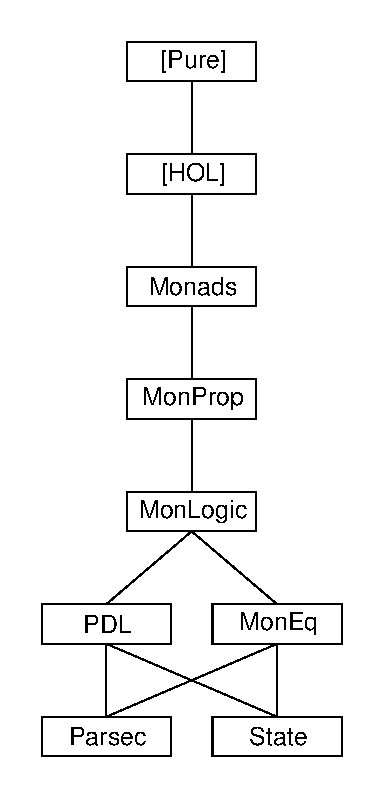
\includegraphics[width=0.35\textwidth]{session_graph}
  \caption{Dependency graph of the Isabelle theories}
  \label{fig:session-graph}
\end{figure}

\section{Monads in Isabelle}
\label{sec:monads-isabelle}
While in Haskell the common ground of all (computable) monads can at least be
captured at the level of operation types\footnote{which is done by making the
  respective type constructors like \texttt{[]} (being syntactical sugar for
  \texttt{List}), \texttt{Maybe}, etc., instances of the constructor class
  \texttt{Monad}}, Isabelle's concept of \emph{axiomatic type classes} is not
strong enough to suit this purpose.  Axiomatic type classes are like Haskell's
type classes, with the supplementary possibility of specifying what properties
the operations over a certain type class must satisfy. For example, the type
class $\Type{parord}$ of partial orders requires its instances to provide the
operations $<$ and $\leq$, but additionally demands that the latter satisfies the
usual properties of transitivity, reflexivity and antisymmetry. For the
specification of monads however one does not require a class of types but rather
a class of type constructors, namely the class of all those type constructors
mapping a given base type into the type of specific computations over this type.

Due to the lack of this concept our implementation simply declares a
polymorphic abstract type $\ivar{a}\ T$, where $T$ is supposed to stand for
the monad in question. This way of proceeding precludes the exact definition of
concrete monads and their primitive operations, since the structure of the monad
is not visible. From the viewpoint of Isabelle's \emph{definitional approach}
-- where HOL is supposed to be supplemented only by further definitions and
theorems rather than axioms -- this may be considered an imperfection, because
additional operations acting on the structure of the monad have to be described
axiomatically. For instance, there will be no way to define what precisely the
operations of writing to or reading a reference in the state monad do, but these
can only be described via their logical effects.  Nonetheless, the way
chosen here adheres to the one suggested in \cite{SchroederMossakowski:PDL} and,
in any case, the alternative would have been to have distinct base theories for
all concrete monads, which is hard to maintain and tedious to implement.

\begin{isabellebody}
\isanewline
\isamarkuptrue%
\isacommand{typedecl}\ {\isacharprime}a\ T\isanewline
\isanewline
\isamarkupfalse%
\isamarkuptrue%
\isacommand{consts}\isanewline
\ bind\ {\isacharcolon}{\isacharcolon}\ {\isachardoublequote}{\isacharprime}a\ T\ {\isasymRightarrow}\ {\isacharparenleft}{\isacharprime}a\ {\isasymRightarrow}\ {\isacharprime}b\ T{\isacharparenright}\ {\isasymRightarrow}\ {\isacharprime}b\ T{\isachardoublequote}\ \ \ \ \ {\isacharparenleft}\isakeyword{infixl}\ {\isachardoublequote}{\isasymggreater}{\isacharequal}{\isachardoublequote}\ {\isadigit{2}}{\isadigit{0}}{\isacharparenright}\isanewline
\ ret\ \ {\isacharcolon}{\isacharcolon}\ {\isachardoublequote}{\isacharprime}a\ {\isasymRightarrow}\ {\isacharprime}a\ T{\isachardoublequote}\isanewline
\isanewline
\isamarkupfalse%
\isacommand{constdefs}\isanewline
\ seq\ {\isacharcolon}{\isacharcolon}\ {\isachardoublequote}{\isacharprime}a\ T\ {\isasymRightarrow}\ {\isacharprime}b\ T\ {\isasymRightarrow}\ {\isacharprime}b\ T{\isachardoublequote}\ \ \ \ \ \ \ \ \ \ \ \ {\isacharparenleft}\isakeyword{infixl}\ {\isachardoublequote}{\isasymggreater}{\isachardoublequote}\ {\isadigit{2}}{\isadigit{0}}{\isacharparenright}\isanewline
\ {\isachardoublequote}p\ {\isasymggreater}\ q\ {\isasymequiv}\ {\isacharparenleft}p\ {\isasymggreater}{\isacharequal}\ {\isacharparenleft}{\isasymlambda}x{\isachardot}\ q{\isacharparenright}{\isacharparenright}{\isachardoublequote}\isamarkupfalse%
\isanewline%
\end{isabellebody}
This is the concrete Isabelle notation for the introduction of the type
$\ivar{a}\ T$ of monadic programs and the basic operations $\op{bind}$, $\ret$
and $\op{seq}$, where the latter is defined in terms of the binding. The
so-called \emph{mixfix annotations} on the right margin declare infix notation,
$\bindOp$ for $\op{bind}$ and $\seqOp$ for $\op{seq}$, which in their simple
form given here resemble the syntax annotations for infix operators in Haskell.
As stated above $\op{bind}$ and $\ret$ can only be declared as abstract
constants through a \textbf{consts} declaration, while $\op{seq}$ can be given a
declaration as well as a concrete definition (albeit in terms of the abstractly
defined operation $\op{bind}$, of course) through the \textbf{constdefs}
statement. The latter combines the effects of the statements \textbf{consts} and
\textbf{defs}, where the \textbf{defs} statement serves the purpose of providing
a definition for a previously introduced constant.

The following is a specification of the monad laws of Equation~(\ref{eq:mondef})
in Isabelle. The \emph{[simp]} instruction makes Isabelle hand a theorem
or axiom to the simplifier as a rewrite rule automatically. We have included a
specification that $\ret$ is injective. From these axioms
we can prove the associativity of $\seqOp$ immediately.
\begin{isabellebody}
\isanewline
\isamarkuptrue%
\isacommand{axioms}\isanewline
\ bind{\isacharunderscore}assoc\ {\isacharbrackleft}simp{\isacharbrackright}{\isacharcolon}\ {\isachardoublequote}{\isacharparenleft}p\ {\isasymggreater}{\isacharequal}\ {\isacharparenleft}{\isasymlambda}x{\isachardot}\ f\ x\ {\isasymggreater}{\isacharequal}\ g{\isacharparenright}{\isacharparenright}\ {\isacharequal}\ {\isacharparenleft}p\ {\isasymggreater}{\isacharequal}\ f\ {\isasymggreater}{\isacharequal}\ g{\isacharparenright}{\isachardoublequote}\isanewline
\ ret{\isacharunderscore}lunit\ {\isacharbrackleft}simp{\isacharbrackright}{\isacharcolon}\ {\isachardoublequote}{\isacharparenleft}ret\ x\ {\isasymggreater}{\isacharequal}\ f{\isacharparenright}\ {\isacharequal}\ f\ x{\isachardoublequote}\isanewline
\ ret{\isacharunderscore}runit\ {\isacharbrackleft}simp{\isacharbrackright}{\isacharcolon}\ {\isachardoublequote}{\isacharparenleft}p\ {\isasymggreater}{\isacharequal}\ ret{\isacharparenright}\ {\isacharequal}\ p{\isachardoublequote}\isanewline
\ ret{\isacharunderscore}inject{\isacharcolon}\ {\isachardoublequote}ret\ x\ {\isacharequal}\ ret\ z\ {\isasymLongrightarrow}\ x\ {\isacharequal}\ z{\isachardoublequote}\isanewline
\isanewline
\isamarkupfalse%
\isacommand{lemma}\ seq{\isacharunderscore}assoc\ {\isacharbrackleft}simp{\isacharbrackright}{\isacharcolon}\ {\isachardoublequote}{\isacharparenleft}p\ {\isasymggreater}\ {\isacharparenleft}q\ {\isasymggreater}\ r{\isacharparenright}{\isacharparenright}\ {\isacharequal}\ {\isacharparenleft}p\ {\isasymggreater}\ q\ {\isasymggreater}\ r{\isacharparenright}{\isachardoublequote}\isanewline
\ \isamarkupfalse%
\isacommand{by}\ {\isacharparenleft}simp\ add{\isacharcolon}\ seq{\isacharunderscore}def{\isacharparenright}\isamarkupfalse%
\isanewline%
\end{isabellebody}

\subsection{The do-Notation}
Next comes the setup of the do-notation by means of Isabelle's syntax
translation facility. This basically is a term-rewriting mechanism on abstract
syntax trees which can be configured by adding rewrite rules for either the
transformation of concrete input into a valid Isabelle term or vice versa. We
will not go into the details of this mechanism, which is laid out in the
Isabelle reference manual \cite{IsaRef04}. The implementation can be found in
Appendix~\ref{cha:isabelle-theories}, p.~\pageref{isa:do-notation}.

The syntax translations make it possible to write monadic programs in a much
more convenient way that mirrors the sequentiality inherent in these programs.
In the implementation we make use of this notation exclusively.  As an example,
one may write the following
\begin{align*}
& \DoStmt{x\leteq p; q\ x} && \DoStmt{x\leteq p; y\leteq q; r\ x\ y} &&
  \DoStmt{x\leteq p; y\leteq q; z\leteq r; \ret~(x,y,z)}\\
\intertext{instead of }
& p \bindOp \LambdaTerm{x}{q\ x}  && 
  p \bindOp (\LambdaTerm{x}{q\bindOp \LambdaTerm{y}{r\ x\ y}}) &&
  \DoStmt{x\leteq p;\DoStmt{y\leteq q; \DoStmt{z\leteq r; \ret~(x,y,z)}}}
\end{align*}
where the third column indicates that multiple
bindings may be input as a sequence rather than in a nested fashion. 
\begin{rem}
  The fact that do-terms are simply syntactical sugar also means that we do not
  formalise the inference rules of the meta-language for monads described in
  Section~\ref{sec:metalanguage-monads}, but rather work with monadic programs
  and their properties directly and just display them in the more convenient
  do-notation. That such a translation can be achieved purely by syntax
  transformations indicates how closely the meta-language is related to actual
  monadic programs.
\end{rem}


\subsection{Properties of Monadic Programs}
\label{sec:isa-prop-monad-progr}

Our main goal for now is to obtain a subtype $\ivar{a}\ D$ of deterministically
side effect free (\emph{dsef}) programs over $\ivar{a}\ T$ so that programs of
type $\Type{bool}\ D$ can be used as formulae of our logic. The kind of
subtyping supported by Isabelle proceeds by defining a new type in terms of a
subset of elements of an existing type. Isabelle then generates a bijection
between this subset of the existing type and the new type which consists of an
\emph{abstraction function} from the existing type into the new one -- which is
only sensibly defined for elements that really have a corresponding element in
the new type -- and a \emph{representation function} mapping elements of the
new type back to their representatives in the existing type. 

It is
straightforward to formalise the concepts of discardability and copyability, the
concepts on which the property $\op{dsef}$ builds. The latter is itself defined
in terms of the former ones as follows.

\begin{isabellebody}
\isamarkuptrue%
\isanewline
\isacommand{constdefs}\isanewline
\ \ dis\ {\isacharcolon}{\isacharcolon}\ {\isachardoublequote}{\isacharprime}a\ T\ {\isasymRightarrow}\ bool{\isachardoublequote}\isanewline
\ \ {\isachardoublequote}dis{\isacharparenleft}p{\isacharparenright}\ {\isasymequiv}\ {\isacharparenleft}do\ {\isacharbraceleft}x{\isasymleftarrow}p{\isacharsemicolon}\ ret{\isacharparenleft}{\isacharparenright}{\isacharbraceright}{\isacharparenright}\ {\isacharequal}\ ret\ {\isacharparenleft}{\isacharparenright}{\isachardoublequote}\isanewline
\isanewline
\ \ cp\ \ {\isacharcolon}{\isacharcolon}\ {\isachardoublequote}{\isacharprime}a\ T\ {\isasymRightarrow}\ bool{\isachardoublequote}\isanewline
\ \ {\isachardoublequote}cp{\isacharparenleft}p{\isacharparenright}\ {\isasymequiv}\ {\isacharparenleft}do\ {\isacharbraceleft}x{\isasymleftarrow}p{\isacharsemicolon}\ y{\isasymleftarrow}p{\isacharsemicolon}\ ret{\isacharparenleft}x{\isacharcomma}y{\isacharparenright}{\isacharbraceright}{\isacharparenright}\ {\isacharequal}\ {\isacharparenleft}do\ {\isacharbraceleft}x{\isasymleftarrow}p{\isacharsemicolon}\ ret{\isacharparenleft}x{\isacharcomma}x{\isacharparenright}{\isacharbraceright}{\isacharparenright}{\isachardoublequote}\isanewline
\isanewline
\ \ dsef\ {\isacharcolon}{\isacharcolon}\ {\isachardoublequote}{\isacharprime}a\ T\ {\isasymRightarrow}\ bool{\isachardoublequote}\isanewline
\ \ {\isachardoublequote}dsef{\isacharparenleft}p{\isacharparenright}\ {\isasymequiv}\ cp{\isacharparenleft}p{\isacharparenright}\ {\isasymand}\ dis{\isacharparenleft}p{\isacharparenright}\ {\isasymand}\ {\isacharparenleft}{\isasymforall}q{\isacharcolon}{\isacharcolon}bool\ T{\isachardot}\ cp{\isacharparenleft}q{\isacharparenright}\ {\isasymand}\ dis{\isacharparenleft}q{\isacharparenright}\ {\isasymlongrightarrow}\ \isanewline
\ \ \ \ \ \ \ \ \ \ \ \ \ \ \ \ \ \ \ \ \ \ \ \ \ \ \ \ \ \ \ \ \ \ \ \
cp{\isacharparenleft}do\
{\isacharbraceleft}x{\isasymleftarrow}p{\isacharsemicolon}\
y{\isasymleftarrow}q{\isacharsemicolon}\
ret{\isacharparenleft}x{\isacharcomma}y{\isacharparenright}{\isacharbraceright}{\isacharparenright}{\isacharparenright}{\isachardoublequote}\isanewline
\end{isabellebody}

The definition of $\op{dsef}$ deserves explanation for two reasons. First, it
should be repeated that there are three equivalent formulations of what it means
for a program to commute with some other program (cf. Def.~\ref{defn:commutes}),
from which we have chosen (\ref{eq:commutes-1}). Second, this formulation
restricts the types of programs that the given program $p$ has to commute with
to those of type $\Type{bool}$ (see also Definition~\ref{defn:dsef} and
Remark~\ref{rem:isa-type-restr}). This is required because Isabelle\footnote{to
  be precise, this statement is only true for logics like HOL which inherit
  their type mechanism from Isabelle's meta-logic} does not allow for a
quantification over type variables in a definition. But this is exactly what
would be done, if implicitly, in the case that the right-hand side of the
definition mentioned an arbitrary program $q :: \ivar{a}\ T$. As $\ivar{a}$
would be arbitrary, any type might serve as an instantiation. An explicit lemma
\irule{commute-bool-arb} is needed to derive the commutativity of a certain
program $p$ with copyable and discardable programs of \emph{any} type from the
commutativity of $p$ among copyable and discardable programs of type
$\Type{bool}$. Because the implementation of global dynamic judgements was the
subject of a different diploma thesis, this `lemma' is in fact provided as an
axiom in this thesis; given a more elaborate infrastructure, it would however be
provable.

Several properties of copyable and discardable programs discussed in
Section~\ref{sec:dl-prelim} have been formalised, the most frequently employed
of which are Lemmas~\ref{thm:dis-general} and \ref{thm:cp-general}
\begin{isabellebody}
\isanewline
\isamarkuptrue%
\isacommand{lemma}\ cp{\isacharunderscore}arb{\isacharcolon}\
{\isachardoublequote}cp\ p\ {\isasymLongrightarrow}\ do\
{\isacharbraceleft}x{\isasymleftarrow}p{\isacharsemicolon}\
y{\isasymleftarrow}p{\isacharsemicolon}\ r\ x\ y{\isacharbraceright}\
{\isacharequal}\ do\ {\isacharbraceleft}x{\isasymleftarrow}p{\isacharsemicolon}\
r\ x\ x{\isacharbraceright}{\isachardoublequote}\isanewline
\isacommand{lemma}\ dis{\isacharunderscore}left{\isacharcolon}\ {\isachardoublequote}dis{\isacharparenleft}p{\isacharparenright}\ {\isasymLongrightarrow}\ do\ {\isacharbraceleft}p{\isacharsemicolon}\ q{\isacharbraceright}\ {\isacharequal}\ q{\isachardoublequote}\isanewline
\isamarkupfalse%
\end{isabellebody}
\noindent Notice how the substitution of $x$ for $y$ in $r$ of lemma
\irule{cp-arb} is achieved by making $r$ a function of $x$ and $y$.
With the above definitions and lemmas at our disposal the type
$\ivar{a}\ D$ can be defined. 

\begin{isabellebody}
\isanewline
\isamarkuptrue%
\isacommand{typedef}\ {\isacharparenleft}Dsef{\isacharparenright}\ {\isacharparenleft}{\isacharprime}a{\isacharparenright}\ D\ {\isacharequal}\ {\isachardoublequote}{\isacharbraceleft}p{\isacharcolon}{\isacharcolon}{\isacharprime}a\ T{\isachardot}\ dsef\ p{\isacharbraceright}{\isachardoublequote}\isanewline
\ \ \isamarkupfalse%
\isacommand{apply}{\isacharparenleft}rule\ exI{\isacharbrackleft}of\ {\isacharunderscore}\ {\isachardoublequote}ret\ x{\isachardoublequote}{\isacharbrackright}{\isacharparenright}\isanewline
\ \ \isamarkupfalse%
\isacommand{apply}{\isacharparenleft}blast\ intro{\isacharcolon}\ dsef{\isacharunderscore}ret{\isacharparenright}\isanewline
\isamarkupfalse%
\isacommand{done}\isamarkupfalse%
\isanewline%
\end{isabellebody}

The proof obligation in the type definition arises due to the
restriction that types must not be empty. We use the program $\ret~x$ as a
witness, since stateless programs are always dsef. This fact has of course been
proved as lemma $\irule{dsef-ret}$ in Isabelle beforehand.
 The \textbf{typedef} statement declares the new
type $\ivar{a}\ D$ to be in bijective correspondence to the set $\op{Dsef}$ of
dsef programs in $\ivar{a}\ T$. The definition of this set is subsequently
available under the name $\irule{Dsef-def}$. What's more, two functions
$\ifun{Abs-Dsef} :: \ivar{a}\ T \Rightarrow \ivar{a}\ D$ and $\ifun{Rep-Dsef} :: \ivar{a}\
D \Rightarrow \ivar{a}\ T$ are generated that mediate between these two types. As the
functions may appear quite often in certain formulae, two abbreviations are
introduced: $\Uparrow p$ stands for $\ifun{Abs-Dsef}\ p$ and $\Downarrow P$ stands for
$\ifun{Rep-Dsef}\ P$. This is quite suggestive, in particular in those cases
where terms of the form $\Uparrow \Downarrow P$ or $\Downarrow \Uparrow p$ appear since one is visually reminded
that these operations cancel each other out.

\begin{rem} \label{rem:cast-ret-isabelle} The reason why terms of the form $\Uparrow p$
  will appear is that one may only write monadic programs in $T$, while
  the formulae of our logic live in $D$. This means that a compound
  truth-valued program $p = \DoStmt{x_1\leteq p_1; \cdots; x_n\leteq p_n; r\ x_1 \cdots
    x_n}$ that is dsef will nonetheless have type $\Type{bool}\ T$. This program
  has to be shifted to $\Type{bool}\ D$ to form the monadic formula $\Uparrow p$.
  Furthermore, there are several atomic programs -- with $\ret~x$ being the
  predominant one -- which are dsef and hence may appear in formulae when
  shifted. We initiate the convention of defining a formula $\op{Prog}
  \equiv\; \Uparrow \op{prog}$ for each atomic dsef program $\op{prog}$. Hence the shifted
  version of $\ret$ is $\op{Ret}:: \ivar{a} \Rightarrow \ivar{a}\ D$.
\end{rem}

Theory MonProp also contains proofs of characteristic properties of dsef
programs which are not shared by discardable or copyable programs. The two most
important facts are that neighbouring dsef programs may be swapped (Theorem
\irule{commute-dsef}, p.~\pageref{isa:commute-dsef}) and that dsef programs
are stable under sequential composition (Theorem \irule{dsef-seq},
p.~\pageref{isa:dsef-seq}). While the first one is quite immediate from the
definitions, the second one asks for a bit more work. 
\begin{isabellebody}
\isanewline
\isacommand{theorem}\ dsef{\isacharunderscore}seq{\isacharcolon}\ {\isachardoublequote}{\isasymlbrakk}dsef\ p{\isacharsemicolon}\ {\isasymforall}x{\isachardot}\ dsef\ {\isacharparenleft}q\ x{\isacharparenright}{\isasymrbrakk}\ {\isasymLongrightarrow}\ dsef\ {\isacharparenleft}do\ {\isacharbraceleft}x{\isasymleftarrow}p{\isacharsemicolon}\ q\ x{\isacharbraceright}{\isacharparenright}{\isachardoublequote}\isanewline
\end{isabellebody}

According to the definition of $\op{dsef}$ proving that $\DoStmt{x\leteq p; q\
  x}$ (call it $r$ in the following) is dsef amounts to showing three facts. The
first one is that $r$ is discardable. This follows from the fact that $p$ and
$q\ x$ are discardable for all $x$. The second one, namely that $r$ is copyable,
follows from the fact that $p$ and $q\ x$ commute with each other, so that the
defining equality of copyability holds for $r$ by the copyability of $p$ and $q\
x$. It must be noted here that while we used condition
(\ref{eq:commutes-1})\footnote{stating that the composition of two discardable
  and copyable programs is again copyable} as part of the defining property of
dsef programs, condition (\ref{eq:commutes-3})\footnote{which states the
  property of commutativity more instructively by actually swapping two
  programs} can easily be inferred from (\ref{eq:commutes-1}), a point that has
been shown in lemma \irule{commute-1-3}. The final fact to be shown is that
$r$ commutes with all copyable and discardable $\Type{bool}$-valued programs.
This follows similarly to the second fact, noting that $p$ and $q\ x$ alone
commute with all discardable and copyable $\Type{bool}$-valued programs.

\subsection{Equational Reasoning in Isar}
\label{sec:eq-reason-isar}
We will now shortly explain how Isar supports equational reasoning. As it is
used in this thesis, equational reasoning means reasoning by chains of
equations, where each separate step is justified mainly by substituting equals
for equals. Take the following lemma, representing the formalisation of how to
infer (\ref{eq:commutes-2}) from (\ref{eq:commutes-1}), as an example.

\begin{isabellebody}
\isanewline
\isacommand{lemma}\ commute{\isacharunderscore}{\isadigit{1}}{\isacharunderscore}{\isadigit{2}}{\isacharcolon}\ {\isachardoublequote}{\isasymlbrakk}cp\ q{\isacharsemicolon}\ cp\ p{\isacharsemicolon}\ dis\ q{\isacharsemicolon}\ dis\ p{\isasymrbrakk}\ {\isasymLongrightarrow}\ cp\ {\isacharparenleft}do\ {\isacharbraceleft}x{\isasymleftarrow}p{\isacharsemicolon}\ y{\isasymleftarrow}q{\isacharsemicolon}\ ret{\isacharparenleft}x{\isacharcomma}y{\isacharparenright}{\isacharbraceright}{\isacharparenright}\isanewline
\ \ \ \ \ \ \ \ \ \ \ \ \ \ \ \ \ \ \ \ {\isasymLongrightarrow}\ do\ {\isacharbraceleft}x{\isasymleftarrow}p{\isacharsemicolon}\ y{\isasymleftarrow}q{\isacharsemicolon}\ ret{\isacharparenleft}x{\isacharcomma}y{\isacharparenright}{\isacharbraceright}\ {\isacharequal}\ do\ {\isacharbraceleft}y{\isasymleftarrow}q{\isacharsemicolon}\ x{\isasymleftarrow}p{\isacharsemicolon}\ ret{\isacharparenleft}x{\isacharcomma}y{\isacharparenright}{\isacharbraceright}{\isachardoublequote}\isanewline
\isamarkupfalse%
\isacommand{proof}\ {\isacharminus}\isanewline
\ \ \isamarkupfalse%
\isacommand{assume}\ a{\isacharcolon}\ {\isachardoublequote}cp\ q{\isachardoublequote}\ {\isachardoublequote}cp\ p{\isachardoublequote}\ {\isachardoublequote}dis\ q{\isachardoublequote}\ {\isachardoublequote}dis\ p{\isachardoublequote}\isanewline
\ \ \isamarkupfalse%
\isacommand{assume}\ c{\isacharcolon}\ {\isachardoublequote}cp\ {\isacharparenleft}do\ {\isacharbraceleft}x{\isasymleftarrow}p{\isacharsemicolon}\ y{\isasymleftarrow}q{\isacharsemicolon}\ ret{\isacharparenleft}x{\isacharcomma}y{\isacharparenright}{\isacharbraceright}{\isacharparenright}{\isachardoublequote}\isanewline
\ \ \isamarkupfalse%
\isacommand{let}\ {\isacharquery}s\ {\isacharequal}\ {\isachardoublequote}do\ {\isacharbraceleft}x{\isasymleftarrow}p{\isacharsemicolon}\ y{\isasymleftarrow}q{\isacharsemicolon}\ ret{\isacharparenleft}x{\isacharcomma}y{\isacharparenright}{\isacharbraceright}{\isachardoublequote}\isanewline
\ \ \isamarkupfalse%
\isacommand{have}\ {\isachardoublequote}{\isacharquery}s\ {\isacharequal}\ do\ {\isacharbraceleft}z{\isasymleftarrow}{\isacharquery}s{\isacharsemicolon}\ ret\ {\isacharparenleft}fst\ z{\isacharcomma}\ snd\ z{\isacharparenright}{\isacharbraceright}{\isachardoublequote}\ \isamarkupfalse%
\isacommand{by}\ simp\isanewline
\ \ \isamarkupfalse%
\isacommand{also}\ \isamarkupfalse%
\isacommand{from}\ c\ \isamarkupfalse%
\isacommand{have}\ {\isachardoublequote}{\isasymdots}\ {\isacharequal}\ do\ {\isacharbraceleft}w{\isasymleftarrow}{\isacharquery}s{\isacharsemicolon}\ z{\isasymleftarrow}{\isacharquery}s{\isacharsemicolon}\ ret\ {\isacharparenleft}fst\ z{\isacharcomma}\ snd\ w{\isacharparenright}{\isacharbraceright}{\isachardoublequote}\ \isamarkupfalse%
\isacommand{by}\ {\isacharparenleft}simp\ add{\isacharcolon}\ cp{\isacharunderscore}arb{\isacharparenright}\isanewline
\ \ \isamarkupfalse%
\isacommand{also}\ \isamarkupfalse%
\isacommand{from}\ a\ \isamarkupfalse%
\isacommand{have}\ {\isachardoublequote}{\isasymdots}\ {\isacharequal}\ do\ {\isacharbraceleft}v{\isasymleftarrow}q{\isacharsemicolon}\ x{\isasymleftarrow}p{\isacharsemicolon}\ ret{\isacharparenleft}x{\isacharcomma}v{\isacharparenright}{\isacharbraceright}{\isachardoublequote}\ \isamarkupfalse%
\isacommand{by}\ {\isacharparenleft}simp\ add{\isacharcolon}\ mon{\isacharunderscore}ctr\ dis{\isacharunderscore}left{\isadigit{2}}{\isacharparenright}\isanewline
\ \ \isamarkupfalse%
\isacommand{finally}\ \isamarkupfalse%
\isacommand{show}\ {\isacharquery}thesis\ \isamarkupfalse%
\isacommand{{\isachardot}}\isanewline
\isamarkupfalse%
\isacommand{qed}\isamarkupfalse%
\isanewline
\end{isabellebody}

\noindent After stating the valid assumptions and setting $?s$ as an
abbreviation for the left-hand side of the equation that is to be shown, a chain
of equations starts beginning with $?s$ and ending with the right-hand side of
the main goal. This kind of successive equational reasoning is realised in Isar
through a sequence of \textbf{have}\ldots \textbf{also have}\ldots statements and a
concluding \textbf{finally} statement. In its simplest form, the \textbf{also}
statement combines two facts of the form $a = b$ and $b = c$ to yield the fact
$a = c$, thus simply exploiting transitivity of equality. The \textbf{finally}
statement reiterates the transitive chain build up so far and feeds it into the
concluding proof -- which in the example is precisely the goal thesis. As a
convenience, three dots `\ldots' within a term refer to the right-hand side of the
most recently established equality. The main workhorse for performing the
intermediate proof steps is the simplifier, since it is ideally suited for
handling equalities and substitution. \cite{BauerWenzel01} contains a detailed
description of extended features of this mechanism, showing how it can also be
applied to  inequalities.


\subsection{Lifting HOL Constants}
\label{sec:lift-hol-const}


The definition of the propositional connectives in Section~\ref{sec:prim-conn}
suggests the introduction of \emph{lifting operators} that allow one to embed
HOL operators into the monadic setting. These lifting operators are well known
from Haskell and their definition in Isabelle does not look that different. The
basic idea is that to apply an $n$-ary operator $f :: [a_1,\ldots,a_n]
\Rightarrow b$ to $n$ monadic programs $p_1 :: a_1\,T, \ldots,  p_n::a_n\,T$, one
simply evaluates these programs in turn and applies the operator to the results.
In principle all HOL operators like equality, comparisons, addition, etc. could
be lifted this way, but for simplicity we will only lift the propositional
connectives and equality in the sequel.

\begin{isabellebody}
\isanewline
\isacommand{constdefs}\isanewline
\ liftM\ {\isacharcolon}{\isacharcolon}\ {\isachardoublequote}{\isacharbrackleft}{\isacharprime}a\ {\isasymRightarrow}\ {\isacharprime}b{\isacharcomma}\ {\isacharprime}a\ T{\isacharbrackright}\ {\isasymRightarrow}\ {\isacharprime}b\ T{\isachardoublequote}\isanewline
\ {\isachardoublequote}liftM\ f\ p\ {\isasymequiv}\ do\ {\isacharbraceleft}x\ {\isasymleftarrow}\ p{\isacharsemicolon}\ ret\ {\isacharparenleft}f\ x{\isacharparenright}{\isacharbraceright}{\isachardoublequote}\isanewline
\ liftM{\isadigit{2}}\ {\isacharcolon}{\isacharcolon}\ {\isachardoublequote}{\isacharbrackleft}{\isacharprime}a\ {\isasymRightarrow}\ {\isacharprime}b\ {\isasymRightarrow}\ {\isacharprime}c{\isacharcomma}\ {\isacharprime}a\ T{\isacharcomma}\ {\isacharprime}b\ T{\isacharbrackright}\ {\isasymRightarrow}\ {\isacharprime}c\ T{\isachardoublequote}\isanewline
\ {\isachardoublequote}liftM{\isadigit{2}}\ f\ p\ q\ {\isasymequiv}\ do\ {\isacharbraceleft}x\ {\isasymleftarrow}\ p{\isacharsemicolon}\ y\ {\isasymleftarrow}\ q{\isacharsemicolon}\ ret\ {\isacharparenleft}f\ x\ y{\isacharparenright}{\isacharbraceright}{\isachardoublequote}\isanewline
\end{isabellebody}

Thanks to lemma \irule{dsef-seq} it is very easy to prove that applying a
lifted operation to dsef programs yields a dsef program:
\begin{isabellebody}
\isanewline
\isacommand{lemma}\ dsef{\isacharunderscore}liftM{\isadigit{2}}{\isacharcolon}\
{\isachardoublequote}{\isasymlbrakk}dsef\ p{\isacharsemicolon}\ dsef\
q{\isasymrbrakk}\ {\isasymLongrightarrow}\ dsef\
{\isacharparenleft}liftM{\isadigit{2}}\ f\ p\
q{\isacharparenright}{\isachardoublequote}\isanewline
\end{isabellebody}
\noindent This fact is essential when introducing the propositional connectives
in this manner, since \EG the conjunction of two formulae is of course required
to be a formula, hence dsef.

\section{Setting up the Logic}
\label{sec:setting-up-logic}

Apart from a slight visual clutter induced by the occurrences of the shifting
functions $\Uparrow$ and $\Downarrow$ the definition of global validity (which we denote here by
a turnstile $\vdash$ instead of the global box $\gbox$) and of the propositional
connectives is now straightforward. We take conjunction, disjunction and
implication as primitives: the constant for falsity does not have do be defined,
since it is available via the injection of $\op{False}$ into the monad, \IE via
$\Ret~\op{False}$.
\begin{isabellebody}
\isanewline
\isacommand{consts}\isanewline
\ {\isachardoublequote}Valid{\isachardoublequote}\ \ \ \ \ \ \ {\isacharcolon}{\isacharcolon}\ {\isachardoublequote}bool\ D\ {\isasymRightarrow}\ bool{\isachardoublequote}\ \ \ \ \ \ \ \ \ \ \ \ \ \ \ {\isacharparenleft}{\isachardoublequote}{\isacharparenleft}{\isasymturnstile}\ {\isacharunderscore}{\isacharparenright}{\isachardoublequote}\ {\isadigit{1}}{\isadigit{5}}{\isacharparenright}\isanewline
\ {\isachardoublequote}{\isasymand}\isactrlsub D{\isachardoublequote}\ \ \ \ \ \ \ \ \ {\isacharcolon}{\isacharcolon}\ {\isachardoublequote}{\isacharbrackleft}bool\ D{\isacharcomma}\ bool\ D{\isacharbrackright}\ {\isasymRightarrow}\ bool\ D{\isachardoublequote}\ \ \ \ \ {\isacharparenleft}\isakeyword{infixr}\ {\isadigit{3}}{\isadigit{5}}{\isacharparenright}\isanewline
\ {\isachardoublequote}{\isasymor}\isactrlsub D{\isachardoublequote}\ \ \ \ \ \ \ \ \ {\isacharcolon}{\isacharcolon}\ {\isachardoublequote}{\isacharbrackleft}bool\ D{\isacharcomma}\ bool\ D{\isacharbrackright}\ {\isasymRightarrow}\ bool\ D{\isachardoublequote}\ \ \ \ \ {\isacharparenleft}\isakeyword{infixr}\ {\isadigit{3}}{\isadigit{0}}{\isacharparenright}\isanewline
\ {\isachardoublequote}{\isasymlongrightarrow}\isactrlsub D{\isachardoublequote}\ \ \ \ \ \ \ \ {\isacharcolon}{\isacharcolon}\ {\isachardoublequote}{\isacharbrackleft}bool\ D{\isacharcomma}\ bool\ D{\isacharbrackright}\ {\isasymRightarrow}\ bool\ D{\isachardoublequote}\ \ \ \ {\isacharparenleft}\isakeyword{infixr}\ {\isadigit{2}}{\isadigit{5}}{\isacharparenright}\isamarkupfalse%
\isanewline
\isacommand{defs}\isanewline
\ \ Valid{\isacharunderscore}def{\isacharcolon}\ {\isachardoublequote}{\isasymturnstile}\ P\ {\isasymequiv}\ {\isasymDown}\ P\ {\isacharequal}\ do\ {\isacharbraceleft}x{\isasymleftarrow}{\isacharparenleft}{\isasymDown}\ P{\isacharparenright}{\isacharsemicolon}\ ret\ True{\isacharbraceright}{\isachardoublequote}\isanewline
\ \ conjD{\isacharunderscore}def{\isacharcolon}\ {\isachardoublequote}P\ {\isasymand}\isactrlsub D\ Q\ {\isasymequiv}\ {\isasymUp}\ {\isacharparenleft}liftM{\isadigit{2}}\ {\isacharparenleft}op\ {\isasymand}{\isacharparenright}\ {\isacharparenleft}{\isasymDown}\ P{\isacharparenright}\ {\isacharparenleft}{\isasymDown}\ Q{\isacharparenright}{\isacharparenright}{\isachardoublequote}\isanewline
\ \ disjD{\isacharunderscore}def{\isacharcolon}\ {\isachardoublequote}P\ {\isasymor}\isactrlsub D\ Q\ {\isasymequiv}\ {\isasymUp}\ {\isacharparenleft}liftM{\isadigit{2}}\ {\isacharparenleft}op\ {\isasymor}{\isacharparenright}\ {\isacharparenleft}{\isasymDown}\ P{\isacharparenright}\ {\isacharparenleft}{\isasymDown}\ Q{\isacharparenright}{\isacharparenright}{\isachardoublequote}\isanewline
\ \ impD{\isacharunderscore}def{\isacharcolon}\ \ {\isachardoublequote}P\ {\isasymlongrightarrow}\isactrlsub D\ Q\ {\isasymequiv}\ {\isasymUp}\ {\isacharparenleft}liftM{\isadigit{2}}\ {\isacharparenleft}op\ {\isasymlongrightarrow}{\isacharparenright}\ {\isacharparenleft}{\isasymDown}\ P{\isacharparenright}\ {\isacharparenleft}{\isasymDown}\ Q{\isacharparenright}{\isacharparenright}{\isachardoublequote}\isanewline
\end{isabellebody}
Other operators like equivalence $\longleftrightarrow$ and negation
$\lnot$ are defined as abbreviations in the usual way:
\begin{isabellebody}
\isanewline
\isacommand{constdefs}\isanewline
\ iffD\ \ \ \ \ \ \ \ {\isacharcolon}{\isacharcolon}\ {\isachardoublequote}{\isacharbrackleft}bool\ D{\isacharcomma}\ bool\ D{\isacharbrackright}\ {\isasymRightarrow}\ bool\ D{\isachardoublequote}\ \ \ {\isacharparenleft}\isakeyword{infixr}\ {\isachardoublequote}{\isasymlongleftrightarrow}\isactrlsub D{\isachardoublequote}\ {\isadigit{2}}{\isadigit{0}}{\isacharparenright}\isanewline
\ {\isachardoublequote}P\ {\isasymlongleftrightarrow}\isactrlsub D\ Q\ {\isasymequiv}\ {\isacharparenleft}P\ {\isasymlongrightarrow}\isactrlsub D\ Q{\isacharparenright}\ {\isasymand}\isactrlsub D\ {\isacharparenleft}Q\ {\isasymlongrightarrow}\isactrlsub D\ P{\isacharparenright}{\isachardoublequote}\isanewline
\ NotD\ \ \ \ \ \ \ \ {\isacharcolon}{\isacharcolon}\ {\isachardoublequote}bool\ D\ {\isasymRightarrow}\ bool\ D{\isachardoublequote}\ \ \ \ \ \ \ \ \ \ \ \ \ \ {\isacharparenleft}{\isachardoublequote}{\isasymnot}\isactrlsub D\ {\isacharunderscore}{\isachardoublequote}\ {\isacharbrackleft}{\isadigit{4}}{\isadigit{0}}{\isacharbrackright}\ {\isadigit{4}}{\isadigit{0}}{\isacharparenright}\isanewline
\ \ {\isachardoublequote}{\isasymnot}\isactrlsub D\ P\ {\isasymequiv}\ P\ {\isasymlongrightarrow}\isactrlsub D\ Ret\ False{\isachardoublequote}\isamarkupfalse%
\isanewline
\end{isabellebody}
The notion of global validity can be simplified, since dsef programs are
discardable. This fact can be stated either as an equality in $T$ or as an
equality in $D$:
\begin{isabellebody}
  \isanewline
  \isacommand{lemma}\ Valid{\isacharunderscore}simp{\isacharcolon}\
  {\isachardoublequote}{\isacharparenleft}{\isasymturnstile}\
  p{\isacharparenright}\ {\isacharequal}\ {\isacharparenleft}{\isasymDown}\ p\
  {\isacharequal}\ ret\ True{\isacharparenright}{\isachardoublequote}\isanewline
  \isacommand{lemma}\ Valid{\isacharunderscore}simpD{\isacharcolon}\ {\isachardoublequote}{\isacharparenleft}{\isasymturnstile}\ P{\isacharparenright}\ {\isacharequal}\ {\isacharparenleft}P\ {\isacharequal}\ Ret\ True{\isacharparenright}{\isachardoublequote}\isanewline
\end{isabellebody}

\begin{rem}
  While the formalisation of the proof calculus as given in
  \cite{SchroederMossakowski:PDL} is tailored towards an intuitionistic
  framework, an immediate consequence of the definitions presented thus far is
  that \emph{the implementation of the calculus in Isabelle is classical}. This
  follows from the fact that the logical operators are defined in terms of the
  HOL operators and that $\Type{bool}$ is classical, \IE contains only two
  values $\op{True}$ and $\op{False}$. A representative theorem confirming that a
  logic is classical is the law of excluded middle. The formulation in the
  monadic setting reads as
  \begin{isabellebody} \isanewline
    \isacommand{theorem}\ pdl{\isacharunderscore}excluded{\isacharunderscore}middle{\isacharcolon}\ {\isachardoublequote}{\isasymturnstile}\ P\ {\isasymor}\isactrlsub D\ {\isacharparenleft}{\isasymnot}\isactrlsub D\ P{\isacharparenright}{\isachardoublequote}\isanewline
  \end{isabellebody}
  The outline of the proof of this theorem is as follows: first, decode $P \lor_D
  (\lnot_D P)$ into the program $\Uparrow \DoStmt{a\leteq \Downarrow P; b\leteq \Downarrow P; \ret~(a \lor \lnot b)}$.
  By copyability of $\Downarrow P$ -- noting that all programs of the form $\Downarrow \Arg$ are
  dsef, therefore copyable -- this program is equal to $\Uparrow \DoStmt{a\leteq \Downarrow P;
    \ret~(a \lor \lnot a)}$. At this point, reasoning in HOL reduces $a \lor \lnot a$ to
  $\op{True}$, so that by discardability of $\Downarrow P$ the whole program is equal to
  $\Ret~\op{True}$, hence globally valid.
\end{rem}

An interesting connection between the $\Ret$ function and every operator
$\op{op}$ that has been lifted by the $\op{liftM*}$ functions to form an
operator $\op{op_D}$ is that $\Ret$ is a homomorphism between
$\op{op}$-terms in HOL and $\op{op_D}$-terms in $D$. This is
reflected by the following equations, which all hinge on the fact that the
operators have simply been lifted.
\begin{isabellebody}
\isanewline
\isacommand{lemma}\ conjD{\isacharunderscore}Ret{\isacharunderscore}hom{\isacharcolon}\ {\isachardoublequote}Ret\ {\isacharparenleft}a{\isasymand}b{\isacharparenright}\ {\isacharequal}\ {\isacharparenleft}{\isacharparenleft}Ret\ a{\isacharparenright}\ {\isasymand}\isactrlsub D\ {\isacharparenleft}Ret\ b{\isacharparenright}{\isacharparenright}{\isachardoublequote}\isanewline
\isacommand{lemma}\ impD{\isacharunderscore}Ret{\isacharunderscore}hom{\isacharcolon}\ {\isachardoublequote}Ret\ {\isacharparenleft}a{\isasymlongrightarrow}b{\isacharparenright}\ {\isacharequal}\ {\isacharparenleft}{\isacharparenleft}Ret\ a{\isacharparenright}\ {\isasymlongrightarrow}\isactrlsub D\ {\isacharparenleft}Ret\ b{\isacharparenright}{\isacharparenright}{\isachardoublequote}\isanewline
\isacommand{lemma}\ NotD{\isacharunderscore}Ret{\isacharunderscore}hom{\isacharcolon}\ {\isachardoublequote}Ret\ {\isacharparenleft}{\isasymnot}\ P{\isacharparenright}\ {\isacharequal}\ {\isacharparenleft}{\isasymnot}\isactrlsub D\ {\isacharparenleft}Ret\ P{\isacharparenright}{\isacharparenright}{\isachardoublequote}\isanewline
\end{isabellebody}
\noindent Dual statements hold for disjunction, equivalence and the like.

\subsection{Basic Proof Rules}
Besides theorem \irule{pdl-excluded-middle} there are several other analogues
of proof rules of HOL given in Section~\ref{isa:proof-rules}. These include
modus ponens, introduction and elimination rules for conjunction and
disjunction, some rules concerning negation and so forth. It would thus be
tempting to try and formulate a natural deduction calculus for the propositional
part of the logic. However, this fails at one critical point: the introduction
rule for implication, which might be formulated as
\[
\irule{pdl-impI}\quad ({\vdash P} \Longrightarrow {\vdash Q}) \Longrightarrow {\vdash P \longrightarrow_D Q}
\]
is not provable, and what's worse, not even valid. This is quite obvious, since
one may not expect any relationship between the \emph{global} validity of $P$ and the
global validity of the formula $P \longrightarrow_D Q$. Hence it does not make sense to assume
the global validity of $P$, prove $\vdash Q$ and then conclude that $P\longrightarrow_D Q$ must be
globally valid. It is a common phenomenon that natural deduction systems -- and
the proof calculus for HOL basically is formulated as such -- have to be
modified if they are to be used for modal logics. For simple logics involving
unparameterised modal operators this can be done rather easily (see
\cite{Fitting93}), but it is as yet unclear how it might be accomplished for the
logic discussed here, which includes modal operators for every possible program
sequence. 

The lack of this single rule has quite profound consequences, since the simplest
theorems like $\vdash {P \longrightarrow_D Q \longrightarrow_D P}$ cannot be proved `logically', \IE with the
natural deduction rules. Like every classical tautology this theorem however has
a semantic proof which proceeds in analogy to the proof of \irule{pdl-excluded-middle}
discussed above by unfolding the definition of global validity and then
manipulating the resulting do-terms. Having to step back to the semantic
definition of the connectives when proving valid formulae is not desirable since
this does not lend itself easily to automation and it makes proofs very
unstructured in comparison to those conducted in a proof calculus.  To obtain a
purely Hilbert-style calculus for the propositional part of the logic it would
theoretically suffice to prove an appropriate set of axiom schemes semantically
and then conduct proofs from these axioms by modus ponens. This way of
proceeding would lead to rather cumbersome proofs and substantially blow up the
amount of work required to verify programs of realistic size, so an alternative
solution had to be found.

\subsection{Proving Tautologies Automatically}
The solution that has been adopted in the implementation is to use the
simplifier, \IE to employ the technique of term rewriting, and enhance it in
such a way that it can prove \emph{classical} propositional tautologies
automatically. The first step to this solution is to regard the propositional
part of the logic as a Boolean algebra. It is a standard exercise \cite[Chapter
5]{BlackburnDeRijkeVenema01} to verify that ($\Type{bool}\ D, \land_D, \lor_D,
\Ret~\op{False}, \Ret~\op{True}$) is such an algebra which further gives rise to a
boolean ring, \IE a commutative ring in which all elements are idempotent, \IE
$X^2 = X$ for all $X$. Taking $\land_D$ as the multiplication and exclusive
disjunction\footnote{recall the definition of exclusive disjunction: $A \oplus B \equiv (A
  \land \lnot B) \lor (\lnot A \land B)$} $\oplus_D$ as the addition of the Boolean ring this equation
certainly holds, since $X \land_D X = X$ is valid. All other requirements of a
Boolean ring like distributivity of multiplication over addition, associativity
of these operations etc. are also satisfied. The major insight then is that a
complete set of rewrite rules for ordered rewriting can be given for Boolean
rings.  A complete set of rewrite rules is one that is terminating and
confluent, such that every term can be rewritten into a unique normal form and
it does not matter which path of possible reductions one follows (cf. the
Church-Rosser property of the untyped lambda calculus in
Prop.~\ref{thm:church-rosser} and the description of the simplifier in
Section~\ref{sec:adv-proof-meth}). But this is exactly what is needed to prove a
classical tautology $T$ automatically, since it can then be rewritten to its
normal form $\Ret~\op{True}$, so that proving $\vdash T$ amounts to proving the trivial
statement $\vdash \Ret~\op{True}$. This final proof step can of course be done
automatically, too.

Section~\ref{isa:simp-pdl-taut} presents all rules the simplifier has to be
equipped with to prove tautologies automatically. For shortage of time the rules
were given as axioms, and only some of them were proved as examples on how such
proofs can be carried out. The rules include associativity and commutativity of
$\land_D$ as well as $\oplus_D$, unit laws for $\land_D$ with respect to $\Ret~\op{True}$ and
absorption laws for $\land_D$. Furthermore, the behaviour of $\land_D$ and $\oplus_D$ with
regard to falsity and the distribution of $\land_D$ over $\oplus_D$ are laid out.  All
these laws -- together with translation rules that let all connectives be
expressed through $\land_D$ and $\oplus_D$ plus falsity -- are collected in the rule set
\irule{pdl-taut}. Tautologies are now proved in one fell swoop:
\begin{isabellebody}
\isanewline
\isacommand{lemma}\ {\isachardoublequote}{\isasymturnstile}\ {\isacharparenleft}P\ {\isasymlongrightarrow}\isactrlsub D\ Q{\isacharparenright}\ {\isasymand}\isactrlsub D\ {\isacharparenleft}{\isasymnot}\isactrlsub D\ P\ {\isasymlongrightarrow}\isactrlsub D\ R{\isacharparenright}\ {\isasymlongleftrightarrow}\isactrlsub D\ {\isacharparenleft}P\ {\isasymand}\isactrlsub D\ Q\ {\isasymor}\isactrlsub D\ {\isasymnot}\isactrlsub D\ P\ {\isasymand}\isactrlsub D\ R{\isacharparenright}{\isachardoublequote}\isanewline
\ \ \isamarkupfalse%
\isacommand{by}\ {\isacharparenleft}simp\ only{\isacharcolon}\ pdl{\isacharunderscore}taut\ Valid{\isacharunderscore}Ret{\isacharparenright}\isanewline
\end{isabellebody}


\subsection{Modal Operators and the Proof Calculus}
We will now make up for the definition of the box and diamond operators which
have been overlooked up to this point. Due to the fact that an elaborate
formalisation of global dynamic judgements has been worked out in a different
diploma thesis, the box and diamond operators are in fact not \emph{defined}
through their unique defining property as given in
Proposition~\ref{thm:unique-determ}, but rather treated as abstract constants.

\begin{isabellebody}
\isanewline
\isacommand{consts}\isanewline
\ Box\ {\isacharcolon}{\isacharcolon}\ {\isachardoublequote}{\isacharprime}a\ T\ {\isasymRightarrow}\ {\isacharparenleft}{\isacharprime}a\ {\isasymRightarrow}\ bool\ D{\isacharparenright}\ {\isasymRightarrow}\ bool\ D{\isachardoublequote}\ \ \ \ \ {\isacharparenleft}{\isachardoublequote}{\isacharbrackleft}{\isacharhash}\ {\isacharunderscore}{\isacharbrackright}{\isacharunderscore}{\isachardoublequote}\ {\isacharbrackleft}{\isadigit{0}}{\isacharcomma}\ {\isadigit{1}}{\isadigit{0}}{\isadigit{0}}{\isacharbrackright}\ {\isadigit{1}}{\isadigit{0}}{\isadigit{0}}{\isacharparenright}\isanewline
\ Dmd\ {\isacharcolon}{\isacharcolon}\ {\isachardoublequote}{\isacharprime}a\ T\
{\isasymRightarrow}\ {\isacharparenleft}{\isacharprime}a\ {\isasymRightarrow}\
bool\ D{\isacharparenright}\ {\isasymRightarrow}\ bool\ D{\isachardoublequote}\
\ \ \ \
{\isacharparenleft}{\isachardoublequote}{\isasymlangle}{\isacharunderscore}{\isasymrangle}{\isacharunderscore}{\isachardoublequote}\
{\isacharbrackleft}{\isadigit{0}}{\isacharcomma}\
{\isadigit{1}}{\isadigit{0}}{\isadigit{0}}{\isacharbrackright}\
{\isadigit{1}}{\isadigit{0}}{\isadigit{0}}{\isacharparenright}\isamarkupfalse%
\isanewline
\end{isabellebody}

Each operator maps a program and a formula depending on the return value of the
program into a monadic formula. The syntax annotations make it possible to
write, \EG $\PDLSBox{\DoStmt{x\leteq p; q}}Q$\footnote{the sharp sign `$\#$' is
  needed to disambiguate box formulae from lists, for which the square bracket
  notation is already in use} or $\PDLDmd{\DoStmt{x\leteq p; q}}(\lambda y\bnd P\ y)$
-- note that both $Q$ and $P$ are function predicates depending on the return
value of the entire do-term inside the box or diamond respectively, and
\emph{not} on the variable $x$ bound in these do-terms. This means that the
notion of variable binding that is performed by these operators differs from
that which has been proposed in \cite{SchroederMossakowski:PDL}, where the
multiple bindings that may occur inside a modal operator all constitute variable
binders for the formula in the scope of the operator.

With the help of some intricate syntax translation instructions it becomes
possible to mimic this kind of multiple variable binding in Isabelle. The idea is
to write a sequence of bindings inside the modal operator and use these bound
variables freely in the formula in scope of the operator, like so:
\[ \PDLSBox{x_1\leteq p_1; \cdots; x_n\leteq p_n}{P\ x_1\cdots x_n} \] The binding
sequence is then transformed into an actual do-term by collecting all bound
variables to form a tuple and appending a $\ret$
expression that takes this tuple as its argument.  The free occurrences of these
variables in the formula in the scope of the modal operator become bound by
turning the formula into a lambda abstraction that expects the tuple of
variables as an argument. So the result of translating the above binding
sequence is
\[ \PDLSBox{\DoStmt{x_1\leteq p_1; \cdots; x_n\leteq p_n;
    \ret~(x_1,\ldots,x_n)}}{\LambdaTerm{(x_1,\ldots,x_n)}{P\ x_1\cdots x_n}} \]

The notation thus set up is in particular nice for sequences of length one,
because $\PDLDmd{x\leteq p}{({P\ x}\; \land_D\; {Q\ x})}$ and
$\PDLDmd{p}{(\LambdaTerm{x}{{P\ x}\; \land_D\; {Q\ x}})}$ denote the same formula,
with the former one emphasising the connection between the return value $x$ of
$p$ and its use in the subsequent conjunction.

With the modal operators readily defined, the proof calculus for propositional
dynamic logic can be implemented,
resulting in the following specification.
\begin{isabellebody}
\isanewline
\isacommand{axioms}\isanewline
\ \ pdl{\isacharunderscore}nec{\isacharcolon}\ \ \ {\isachardoublequote}{\isacharparenleft}{\isasymforall}x{\isachardot}\ {\isasymturnstile}\ P\ x{\isacharparenright}\ {\isasymLongrightarrow}\ {\isasymturnstile}\ {\isacharbrackleft}{\isacharhash}\ x{\isasymleftarrow}p{\isacharbrackright}{\isacharparenleft}P\ x{\isacharparenright}{\isachardoublequote}\isanewline
\ \ pdl{\isacharunderscore}mp{\isacharunderscore}{\isacharcolon}\ \ \ \ {\isachardoublequote}{\isasymlbrakk}{\isasymturnstile}\ {\isacharparenleft}P\ {\isasymlongrightarrow}\isactrlsub D\ \ Q{\isacharparenright}{\isacharsemicolon}\ {\isasymturnstile}\ P{\isasymrbrakk}\ {\isasymLongrightarrow}\ {\isasymturnstile}\ Q{\isachardoublequote}
\isanewline
\ \isanewline
\ \ pdl{\isacharunderscore}k{\isadigit{1}}{\isacharcolon}\ \ \ \ {\isachardoublequote}{\isasymturnstile}\ {\isacharbrackleft}{\isacharhash}\ x{\isasymleftarrow}p{\isacharbrackright}{\isacharparenleft}P\ x\ {\isasymlongrightarrow}\isactrlsub D\ Q\ x{\isacharparenright}\ {\isasymlongrightarrow}\isactrlsub D\ {\isacharbrackleft}{\isacharhash}\ x{\isasymleftarrow}p{\isacharbrackright}{\isacharparenleft}P\ x{\isacharparenright}\ {\isasymlongrightarrow}\isactrlsub D\ {\isacharbrackleft}{\isacharhash}\ x{\isasymleftarrow}p{\isacharbrackright}{\isacharparenleft}Q\ x{\isacharparenright}{\isachardoublequote}\isanewline
\ \ pdl{\isacharunderscore}k{\isadigit{2}}{\isacharcolon}\ \ \ \ {\isachardoublequote}{\isasymturnstile}\ {\isacharbrackleft}{\isacharhash}\ x{\isasymleftarrow}p{\isacharbrackright}{\isacharparenleft}P\ x\ {\isasymlongrightarrow}\isactrlsub D\ Q\ x{\isacharparenright}\ {\isasymlongrightarrow}\isactrlsub D\ {\isasymlangle}x{\isasymleftarrow}p{\isasymrangle}{\isacharparenleft}P\ x{\isacharparenright}\ {\isasymlongrightarrow}\isactrlsub D\ {\isasymlangle}x{\isasymleftarrow}p{\isasymrangle}{\isacharparenleft}Q\ x{\isacharparenright}{\isachardoublequote}\isanewline
\ \ pdl{\isacharunderscore}k{\isadigit{3}}B{\isacharcolon}\ \ \ {\isachardoublequote}{\isasymturnstile}\ Ret\ P\ {\isasymlongrightarrow}\isactrlsub D\ {\isacharbrackleft}{\isacharhash}\ x{\isasymleftarrow}p{\isacharbrackright}{\isacharparenleft}Ret\ P{\isacharparenright}{\isachardoublequote}\isanewline
\ \ pdl{\isacharunderscore}k{\isadigit{3}}D{\isacharcolon}\ \ \ {\isachardoublequote}{\isasymturnstile}\ {\isasymlangle}x{\isasymleftarrow}p{\isasymrangle}{\isacharparenleft}Ret\ P{\isacharparenright}\ {\isasymlongrightarrow}\isactrlsub D\ Ret\ P{\isachardoublequote}\isanewline
\ \ pdl{\isacharunderscore}k{\isadigit{4}}{\isacharcolon}\ \ \ \ {\isachardoublequote}{\isasymturnstile}\ {\isasymlangle}x{\isasymleftarrow}p{\isasymrangle}{\isacharparenleft}P\ x\ {\isasymor}\isactrlsub D\ Q\ x{\isacharparenright}\ {\isasymlongrightarrow}\isactrlsub D\ {\isacharparenleft}{\isasymlangle}x{\isasymleftarrow}p{\isasymrangle}{\isacharparenleft}P\ x{\isacharparenright}\ {\isasymor}\isactrlsub D\ {\isasymlangle}x{\isasymleftarrow}p{\isasymrangle}{\isacharparenleft}Q\ x{\isacharparenright}{\isacharparenright}{\isachardoublequote}\isanewline
\ \ pdl{\isacharunderscore}k{\isadigit{5}}{\isacharcolon}\ \ \ \ {\isachardoublequote}{\isasymturnstile}\ {\isacharparenleft}{\isasymlangle}x{\isasymleftarrow}p{\isasymrangle}{\isacharparenleft}P\ x{\isacharparenright}\ {\isasymlongrightarrow}\isactrlsub D\ {\isacharbrackleft}{\isacharhash}\ x{\isasymleftarrow}p{\isacharbrackright}{\isacharparenleft}Q\ x{\isacharparenright}{\isacharparenright}\ {\isasymlongrightarrow}\isactrlsub D\ {\isacharbrackleft}{\isacharhash}\ x{\isasymleftarrow}p{\isacharbrackright}{\isacharparenleft}P\ x\ {\isasymlongrightarrow}\isactrlsub D\ Q\ x{\isacharparenright}{\isachardoublequote}\isanewline
\ \ pdl{\isacharunderscore}seqB{\isacharcolon}\ \ {\isachardoublequote}{\isasymturnstile}\ {\isacharbrackleft}{\isacharhash}\ x{\isasymleftarrow}p{\isacharsemicolon}\ y{\isasymleftarrow}q\ x{\isacharbrackright}{\isacharparenleft}P\ x\ y{\isacharparenright}\ {\isasymlongleftrightarrow}\isactrlsub D\ {\isacharbrackleft}{\isacharhash}\ x{\isasymleftarrow}p{\isacharbrackright}{\isacharbrackleft}{\isacharhash}\ y{\isasymleftarrow}q\ x{\isacharbrackright}{\isacharparenleft}P\ x\ y{\isacharparenright}{\isachardoublequote}\isanewline
\ \ pdl{\isacharunderscore}seqD{\isacharcolon}\ \ {\isachardoublequote}{\isasymturnstile}\ {\isasymlangle}x{\isasymleftarrow}p{\isacharsemicolon}\ y{\isasymleftarrow}q\ x{\isasymrangle}{\isacharparenleft}P\ x\ y{\isacharparenright}\ {\isasymlongleftrightarrow}\isactrlsub D\ {\isasymlangle}x{\isasymleftarrow}p{\isasymrangle}{\isasymlangle}y{\isasymleftarrow}q\ x{\isasymrangle}{\isacharparenleft}P\ x\ y{\isacharparenright}{\isachardoublequote}\isanewline
\ \ pdl{\isacharunderscore}ctrB{\isacharcolon}\ \ {\isachardoublequote}{\isasymturnstile}\ {\isacharbrackleft}{\isacharhash}\ x{\isasymleftarrow}p{\isacharsemicolon}\ y{\isasymleftarrow}q\ x{\isacharbrackright}{\isacharparenleft}P\ y{\isacharparenright}\ {\isasymlongrightarrow}\isactrlsub D\ {\isacharbrackleft}{\isacharhash}\ y{\isasymleftarrow}do\ {\isacharbraceleft}x{\isasymleftarrow}p{\isacharsemicolon}\ q\ x{\isacharbraceright}{\isacharbrackright}{\isacharparenleft}P\ y{\isacharparenright}{\isachardoublequote}\isanewline
\ \ pdl{\isacharunderscore}ctrD{\isacharcolon}\ \ {\isachardoublequote}{\isasymturnstile}\ {\isasymlangle}y{\isasymleftarrow}do\ {\isacharbraceleft}x{\isasymleftarrow}p{\isacharsemicolon}\ q\ x{\isacharbraceright}{\isasymrangle}{\isacharparenleft}P\ y{\isacharparenright}\ {\isasymlongrightarrow}\isactrlsub D\ \ {\isasymlangle}x{\isasymleftarrow}p{\isacharsemicolon}\ y{\isasymleftarrow}q\ x{\isasymrangle}{\isacharparenleft}P\ y{\isacharparenright}{\isachardoublequote}\isanewline
\ \ pdl{\isacharunderscore}retB{\isacharcolon}\ \ {\isachardoublequote}{\isasymturnstile}\ {\isacharbrackleft}{\isacharhash}\ x{\isasymleftarrow}ret\ a{\isacharbrackright}{\isacharparenleft}P\ x{\isacharparenright}\ {\isasymlongleftrightarrow}\isactrlsub D\ P\ a{\isachardoublequote}\isanewline
\ \ pdl{\isacharunderscore}retD{\isacharcolon}\ \ {\isachardoublequote}{\isasymturnstile}\ {\isasymlangle}x{\isasymleftarrow}ret\ a{\isasymrangle}{\isacharparenleft}P\ x{\isacharparenright}\ {\isasymlongleftrightarrow}\isactrlsub D\ P\ a{\isachardoublequote}\isanewline
\ \ pdl{\isacharunderscore}dsefB{\isacharcolon}\ {\isachardoublequote}dsef\ p\ {\isasymLongrightarrow}\ {\isasymturnstile}\ {\isasymUp}\ {\isacharparenleft}do\ {\isacharbraceleft}a{\isasymleftarrow}p{\isacharsemicolon}\ {\isasymDown}\ {\isacharparenleft}P\ a{\isacharparenright}{\isacharbraceright}{\isacharparenright}\ {\isasymlongleftrightarrow}\isactrlsub D\ {\isacharbrackleft}{\isacharhash}\ a{\isasymleftarrow}p{\isacharbrackright}{\isacharparenleft}P\ a{\isacharparenright}{\isachardoublequote}\isanewline
\ \ pdl{\isacharunderscore}dsefD{\isacharcolon}\ {\isachardoublequote}dsef\ p\ {\isasymLongrightarrow}\ {\isasymturnstile}\ {\isasymUp}\ {\isacharparenleft}do\ {\isacharbraceleft}a{\isasymleftarrow}p{\isacharsemicolon}\ {\isasymDown}\ {\isacharparenleft}P\ a{\isacharparenright}{\isacharbraceright}{\isacharparenright}\ {\isasymlongleftrightarrow}\isactrlsub D\ {\isasymlangle}a{\isasymleftarrow}p{\isasymrangle}{\isacharparenleft}P\ a{\isacharparenright}{\isachardoublequote}\isamarkupfalse%
\isanewline
\end{isabellebody}

This specification does not look all that different from the original one
presented in Figure~\ref{fig:mon-dyn-logic}. The side-condition in the
necessitation rule that variable $x$ must not occur free in the assumptions can
be formalised by requiring that $P\ x$ holds for all $x$, since this precludes
any assumptions to be made on $x$. The $K$ axioms really are almost identical to
the original specification. The axioms for dsef programs, \irule{pdl-dsefB} and
\irule{pdl-dsefD}, cannot be stated in the convenient notation in which dsef
programs of type $\ivar{a}\ T$ are simply substituted for actual values of type
$\ivar{a}$, since this results in a type error. So in the specification one has
to resort to the decoded forms, where the dsef program is evaluated first, and
the resulting value $a$ is used in the formula $P\ a$.

For the structural rules there also do not appear to be notable differences, but
this is not quite true: the syntax translations transform, \EG, the depicted
formula \irule{pdl-seqB}
\[ \PDLSBox{x\leteq p; y\leteq q\ x}{P\ x\ y} \longleftrightarrow_D \PDLSBox{x\leteq p}{\PDLSBox{y\leteq
    q\ x}{P\ x\ y}}
\]
into the genuine Isabelle term
\[
\PDLSBox{\DoStmt{x\leteq p; y\leteq q\ x; \ret~(x,y)}}{\LambdaTerm{(x,y)}{P\ x\
    y}} \longleftrightarrow_D \PDLSBox{p}{\LambdaTerm{x}{\PDLSBox{q\ x}{\LambdaTerm{y}{P\ x\ y}}}}
\]
which has a rather complicated structure. This complexity and the fact that the $\ret$
expression only appears on the left-hand side of the equivalence will make it
hard to apply the axiom in actual proofs about compound programs, because these
will hardly ever unify with the program structure imposed by the axiom.

It has been shown in \cite{SchroederMossakowski:PDL} that simple monads (cf.
Rem.~\ref{rem:simple-monads}) satisfy the converses of the contraction axioms
\irule{pdl-ctrB} and \irule{pdl-ctrD}, \IE the same formulae with the
implication arrows reversed.  These converse axioms make it possible to prove
simplified versions of the sequencing axioms which have turned out to be more
effective in practice. Whether there is a proof for these theorems in monads
that are not simple, too, is currently unclear. For the box operator the
corresponding theorem is
\begin{isabellebody}
\isanewline
\isacommand{axioms}\isanewline
pdl{\isacharunderscore}seqB{\isacharunderscore}simp{\isacharcolon}\ {\isachardoublequote}{\isasymturnstile}\ {\isacharparenleft}\ {\isacharbrackleft}{\isacharhash}\ x{\isasymleftarrow}p{\isacharbrackright}{\isacharbrackleft}{\isacharhash}\ y{\isasymleftarrow}q\ x{\isacharbrackright}{\isacharparenleft}P\ y{\isacharparenright}\ {\isacharparenright}\ {\isasymlongleftrightarrow}\isactrlsub D\ {\isacharparenleft}\ {\isacharbrackleft}{\isacharhash}\ y{\isasymleftarrow}do\ {\isacharbraceleft}x{\isasymleftarrow}p{\isacharsemicolon}\ q\ x{\isacharbraceright}{\isacharbrackright}{\isacharparenleft}P\ y{\isacharparenright}\ {\isacharparenright}{\isachardoublequote}\isamarkupfalse%
\isanewline
\end{isabellebody}

\noindent with the equivalence of $\PDLSBox{x\leteq p; y\leteq q\ x}{P\ y}$ and
$\PDLSBox{y\leteq \DoStmt{x\leteq p; q\ x}}{P\ y}$ being the key fact required for
the proof. This equivalence is precisely what is provided by the contraction
rules and their converses.

Although the simpler rendition of the sequencing axiom does not allow for reasoning
about intermediate results -- as $P$ only depends on the return value of $q\ x$,
but not that of $p$ -- one has to remember that in rule \irule{pdl-seqB} the
intermediate results are only made available to $P$ by packing all of them into
a tuple $\bar x$ and making $\ret~\bar x$ the final expression of the do-term.
The formulation as given in \irule{pdl-seqB-simp} is more flexible, since $q\ x$
may or may not consist of or at least end with such a $\ret$ expression. In the
case where one is in fact not interested in the value of $x$ (\EG when nothing
is to be said about intermediate results), it turns out to be more convenient to
dispose of the final $\ret$ expression. And the general contraction rules are
too weak to make this possible when working with \irule{pdl-seqB}. Given some
further rules that will be described below it is easily possible to employ
\irule{pdl-seqB-simp} to prove theorems about the equivalence of multiply split
boxes and their `joint box':
\begin{isabellebody}
\isanewline
\isacommand{lemma}\ {\isachardoublequote}{\isasymturnstile}\ {\isacharbrackleft}{\isacharhash}\ do\ {\isacharbraceleft}x{\isadigit{1}}{\isasymleftarrow}p{\isadigit{1}}{\isacharsemicolon}\ x{\isadigit{2}}{\isasymleftarrow}p{\isadigit{2}}{\isacharsemicolon}\ x{\isadigit{3}}{\isasymleftarrow}p{\isadigit{3}}{\isacharsemicolon}\ r\ x{\isadigit{1}}\ x{\isadigit{2}}\ x{\isadigit{3}}{\isacharbraceright}{\isacharbrackright}P\ {\isasymlongleftrightarrow}\isactrlsub D\isanewline
\ \ \ \ \ \ \ \ \ {\isacharbrackleft}{\isacharhash}\ x{\isadigit{1}}{\isasymleftarrow}p{\isadigit{1}}{\isacharbrackright}{\isacharbrackleft}{\isacharhash}\ x{\isadigit{2}}{\isasymleftarrow}p{\isadigit{2}}{\isacharbrackright}{\isacharbrackleft}{\isacharhash}\ x{\isadigit{3}}{\isasymleftarrow}p{\isadigit{3}}{\isacharbrackright}{\isacharbrackleft}{\isacharhash}\ r\ x{\isadigit{1}}\ x{\isadigit{2}}\ x{\isadigit{3}}{\isacharbrackright}P{\isachardoublequote}\isanewline
\end{isabellebody}

\subsection{Theorems and Proof Rules Involving Modal Operators}
\label{sec:theorems-proof-rules}

All theorems of Section~\ref{sec:basic-lemmas} -- which include the distribution
of the box operator over finite conjunctions (named \irule{box-conj-imp-distrib}
here), the regularity and weakening rules (\irule{pdl-box-reg},
\irule{pdl-dmd-reg}, \irule{pdl-wkB}, \irule{pdl-wkD}) as well as several
other lemmas -- have also been proved in Isabelle. The proofs thereof are heavily
inspired by how they have been carried out `on paper', so we just refer to
Section~\ref{isa:pdl-derived-rules} in the Appendix for a formal Isabelle
verification.

A more interesting proof which has not been presented before, because it relies on
the underlying logic being classical, is the relationship between the box and
diamond operator. It has already been stated that the propositional part of the
logic behaves classical, but the following theorem confirms that this is also true
for the relation between the modal operators.
\begin{isabellebody}
\isanewline
\isacommand{theorem}\ dmd{\isacharunderscore}box{\isacharunderscore}rel{\isacharcolon}\ {\isachardoublequote}{\isasymturnstile}\ {\isasymlangle}x{\isasymleftarrow}p{\isasymrangle}{\isacharparenleft}P\ x{\isacharparenright}\ {\isasymlongleftrightarrow}\isactrlsub D\ {\isasymnot}\isactrlsub D\ {\isacharbrackleft}{\isacharhash}\ x{\isasymleftarrow}p{\isacharbrackright}{\isacharparenleft}{\isasymnot}\isactrlsub D\ P\ x{\isacharparenright}{\isachardoublequote}\isanewline
\end{isabellebody}

The formula is proved in two steps, each one validating one direction of the
equivalence. The first half, in which the definition of negation\footnote{$\lnot_D P
  \equiv P \longrightarrow_D \Ret~\op{False}$} has already been unfolded, looks as follows. The
Isar keyword \textbf{is} introduces an abbreviation for the term preceding it.
In the case at hand, $?b$ and $?d$ are matched against and bound to the box and
diamond formulae $\PDLSBox{x\leteq p}{P\ x \longrightarrow_D \Ret~\op{False}}$ and
$\PDLDmd{x\leteq p}{P\ x}$ respectively.
\begin{isabellebody}
\isanewline
\isacommand{lemma}\ dmd{\isacharunderscore}box{\isacharunderscore}rel{\isadigit{1}}{\isacharcolon}\ {\isachardoublequote}{\isasymturnstile}\ {\isacharparenleft}{\isacharbrackleft}{\isacharhash}\ x{\isasymleftarrow}p{\isacharbrackright}{\isacharparenleft}P\ x\ {\isasymlongrightarrow}\isactrlsub D\ Ret\ False{\isacharparenright}\ {\isasymlongrightarrow}\isactrlsub D\ Ret\ False{\isacharparenright}\ {\isasymlongrightarrow}\isactrlsub D\ {\isasymlangle}x{\isasymleftarrow}p{\isasymrangle}{\isacharparenleft}P\ x{\isacharparenright}{\isachardoublequote}\ \isanewline
\ \ {\isacharparenleft}\isakeyword{is}\ {\isachardoublequote}{\isasymturnstile}\ {\isacharparenleft}{\isacharquery}b\ {\isasymlongrightarrow}\isactrlsub D\ Ret\ False{\isacharparenright}\ {\isasymlongrightarrow}\isactrlsub D\ {\isacharquery}d{\isachardoublequote}{\isacharparenright}\isanewline
\isamarkupfalse%
\isacommand{proof}\ {\isacharminus}\isanewline
\ \ \isamarkupfalse%
\isacommand{have}\ {\isachardoublequote}{\isasymturnstile}\ {\isacharparenleft}{\isacharquery}d\ {\isasymlongrightarrow}\isactrlsub D\ Ret\ False{\isacharparenright}\ {\isasymlongrightarrow}\isactrlsub D\ {\isacharquery}b{\isachardoublequote}\ \isanewline
\ \ \isamarkupfalse%
\isacommand{proof}\ {\isacharminus}\isanewline
\ \ \ \ \isamarkupfalse%
\isacommand{have}\ f{\isadigit{1}}{\isacharcolon}\ {\isachardoublequote}{\isasymturnstile}\ {\isacharparenleft}{\isacharparenleft}{\isacharquery}d\ {\isasymlongrightarrow}\isactrlsub D\ {\isacharbrackleft}{\isacharhash}\ x{\isasymleftarrow}p{\isacharbrackright}{\isacharparenleft}Ret\ False{\isacharparenright}{\isacharparenright}\ {\isasymlongrightarrow}\isactrlsub D\ {\isacharquery}b{\isacharparenright}\ {\isasymlongrightarrow}\isactrlsub D\ \isanewline
\ \ \ \ \ \ \ \ \ \ \ \ \ \ \ \ {\isacharparenleft}{\isacharquery}d\ {\isasymlongrightarrow}\isactrlsub D\ Ret\ False{\isacharparenright}\ {\isasymlongrightarrow}\isactrlsub D\ {\isacharquery}b{\isachardoublequote}\isanewline
\ \ \ \ \ \ \isamarkupfalse%
\isacommand{by}\ {\isacharparenleft}simp\ add{\isacharcolon}\ pdl{\isacharunderscore}taut{\isacharparenright}\isanewline
\ \ \ \ \isamarkupfalse%
\isacommand{have}\ f{\isadigit{2}}{\isacharcolon}\ {\isachardoublequote}{\isasymturnstile}\ {\isacharparenleft}{\isacharquery}d\ {\isasymlongrightarrow}\isactrlsub D\ {\isacharbrackleft}{\isacharhash}\ x{\isasymleftarrow}p{\isacharbrackright}{\isacharparenleft}Ret\ False{\isacharparenright}{\isacharparenright}\ {\isasymlongrightarrow}\isactrlsub D\ {\isacharquery}b{\isachardoublequote}\ \isanewline
\ \ \ \ \ \ \isamarkupfalse%
\isacommand{by}\ {\isacharparenleft}rule\ pdl{\isacharunderscore}k{\isadigit{5}}{\isacharparenright}\isanewline
\ \ \ \ \isamarkupfalse%
\isacommand{from}\ f{\isadigit{1}}\ f{\isadigit{2}}\ \isamarkupfalse%
\isacommand{show}\ {\isacharquery}thesis\ \isamarkupfalse%
\isacommand{by}\ {\isacharparenleft}rule\ pdl{\isacharunderscore}mp{\isacharparenright}\isanewline
\ \ \isamarkupfalse%
\isacommand{qed}\isanewline
\ \ \isamarkupfalse%
\isacommand{thus}\ {\isacharquery}thesis\ \isamarkupfalse%
\isacommand{by}\ {\isacharparenleft}simp\ add{\isacharcolon}\ pdl{\isacharunderscore}taut{\isacharparenright}\isanewline
\isamarkupfalse%
\isacommand{qed}\isamarkupfalse%
\isanewline
\end{isabellebody}

The proof proceeds by classical contraposition, \IE instead of proving the
main goal we initially show the following formula
\[
(\PDLDmd{x\leteq p}{(P\ x)} \longrightarrow_D \Ret~\op{False}) \longrightarrow_D \PDLSBox{x\leteq p}{(P\ x
  \longrightarrow_D \Ret~\op{False})}
\]
(call it $\Phi$) to hold and let the simplifier conclude the proof by equalising
$\Phi$ and the main goal with the help of \irule{pdl-taut}. Noticing that $\Phi$
already looks quite similar to an instance of axiom \irule{pdl-k5} -- with only
the leftmost $\Ret$ term to be replaced by the formula $\PDLSBox{x\leteq
  p}{(\Ret~\op{False})}$ -- we recognise that the axiom really implies the goal,
\IE for an appropriate instance $\Psi$ of axiom \irule{pdl-k5} we have that $\Psi \longrightarrow_D
\Phi$ is a tautology that can once again be proved by the simplifier. Hence, a
final application of modus ponens finishes the proof.

The second half of the equivalence is easily proved, as it is tautologically
implied by \irule{pdl-k3D} and \irule{pdl-k2}:
\begin{isabellebody}
\isanewline
\isacommand{lemma}\ dmd{\isacharunderscore}box{\isacharunderscore}rel{\isadigit{2}}{\isacharcolon}\ {\isachardoublequote}{\isasymturnstile}\ {\isasymlangle}x{\isasymleftarrow}p{\isasymrangle}{\isacharparenleft}P\ x{\isacharparenright}\ {\isasymlongrightarrow}\isactrlsub D\ {\isacharbrackleft}{\isacharhash}\ x{\isasymleftarrow}p{\isacharbrackright}{\isacharparenleft}P\ x\ {\isasymlongrightarrow}\isactrlsub D\ Ret\ False{\isacharparenright}\ {\isasymlongrightarrow}\isactrlsub D\ Ret\ False{\isachardoublequote}\isanewline
\isamarkupfalse%
\isacommand{proof}\ {\isacharminus}\isanewline
\ \ \isamarkupfalse%
\isacommand{have}\ {\isachardoublequote}{\isasymturnstile}\ {\isacharparenleft}{\isasymlangle}x{\isasymleftarrow}p{\isasymrangle}{\isacharparenleft}Ret\ False{\isacharparenright}\ {\isasymlongrightarrow}\isactrlsub D\ Ret\ False{\isacharparenright}\ {\isasymlongrightarrow}\isactrlsub D\ \isanewline
\ \ \ \ \ \ \ \ \ \ {\isacharparenleft}{\isacharbrackleft}{\isacharhash}\ x{\isasymleftarrow}p{\isacharbrackright}{\isacharparenleft}P\ x\ {\isasymlongrightarrow}\isactrlsub D\ Ret\ False{\isacharparenright}\ {\isasymlongrightarrow}\isactrlsub D\ {\isasymlangle}x{\isasymleftarrow}p{\isasymrangle}{\isacharparenleft}P\ x{\isacharparenright}\ {\isasymlongrightarrow}\isactrlsub D\ {\isasymlangle}x{\isasymleftarrow}p{\isasymrangle}{\isacharparenleft}Ret\ False{\isacharparenright}{\isacharparenright}\ {\isasymlongrightarrow}\isactrlsub D\ \ \isanewline
\ \ \ \ \ \ \ \ \ \ \ {\isasymlangle}x{\isasymleftarrow}p{\isasymrangle}{\isacharparenleft}P\ x{\isacharparenright}\ {\isasymlongrightarrow}\isactrlsub D\ {\isacharbrackleft}{\isacharhash}\ x{\isasymleftarrow}p{\isacharbrackright}{\isacharparenleft}P\ x\ {\isasymlongrightarrow}\isactrlsub D\ Ret\ False{\isacharparenright}\ {\isasymlongrightarrow}\isactrlsub D\ Ret\ False{\isachardoublequote}\isanewline
\ \ \ \ \isamarkupfalse%
\isacommand{by}\ {\isacharparenleft}simp\ add{\isacharcolon}\ pdl{\isacharunderscore}taut{\isacharparenright}\isanewline
\ \ \isamarkupfalse%
\isacommand{from}\ this\ pdl{\isacharunderscore}k{\isadigit{3}}D\ pdl{\isacharunderscore}k{\isadigit{2}}\ \isamarkupfalse%
\isacommand{show}\ {\isacharquery}thesis\ \isamarkupfalse%
\isacommand{by}\ {\isacharparenleft}rule\ pdl{\isacharunderscore}mp{\isacharunderscore}{\isadigit{2}}x{\isacharparenright}\isanewline
\isamarkupfalse%
\isacommand{qed}\isamarkupfalse%
\end{isabellebody}

\section{A Specification of Parser Combinators}
\label{sec:spec-pars-comb}

In this section it is shown how the monad-independent specification of the
calculus of dynamic logic can be extended by axioms to describe a monad of basic
parser combinators. This specification has been heavily influenced by the
Haskell implementation presented in \cite{HuttonMeijer96}, but in contrast to
that work we specified a \emph{deterministic} parser monad with fall back
alternatives.  The basic operations of this parser are
\begin{isabellebody}
\isanewline
\isacommand{consts}\isanewline
\ \ item\ \ \ \ \ \ \ {\isacharcolon}{\isacharcolon}\ {\isachardoublequote}nat\ T{\isachardoublequote}\ \ \ \ \ \ %
\isanewline
\ \ fail\ \ \ \ \ \ \ {\isacharcolon}{\isacharcolon}\ {\isachardoublequote}{\isacharprime}a\ T{\isachardoublequote}\ \ \ \ \ \ \ %
\isanewline
\ \ alt\ \ \ \ \ \ \ \ {\isacharcolon}{\isacharcolon}\ {\isachardoublequote}{\isacharprime}a\ T\ {\isasymRightarrow}\ {\isacharprime}a\ T\ {\isasymRightarrow}\ {\isacharprime}a\ T{\isachardoublequote}\isanewline
\ \ getInput\ \ \ {\isacharcolon}{\isacharcolon}\ {\isachardoublequote}nat\ list\ T{\isachardoublequote}\ %
\isanewline
\ \ setInput\ \ \ {\isacharcolon}{\isacharcolon}\ {\isachardoublequote}nat\ list\ {\isasymRightarrow}\ unit\ T{\isachardoublequote}\ \isanewline
\end{isabellebody}
\noindent where $\op{item}$ parses exactly one natural number from the finite
stream of input numbers, $\op{fail}$ is a parser that always fails, thus
representing a dead end, the combinator $\op{alt}$ (syntactically sugared by two
parallel bars `$\|$') takes two parsers $p$ and $q$ and yields a parser that
runs the first argument of $\op{alt}$ -- let it be $p$ -- first, and only if it
fails the second parser $q$ is tried. Every producible parser thus always
yields at most one result. Finally there are operations $\op{getInput}$ and
$\op{setInput}$ to read and set the remaining input stream. As a typical
implementation of this monad one might use a deterministic state monad with
an added exception representing failure. 

As an abbreviation we also introduced the operation $\op{eot}$ (for `end of
text') which is defined through $\op{getInput}$ in the obvious way. In
accordance with the convention of Remark~\ref{rem:cast-ret-isabelle} the
operations $\op{Eot}$ and $\op{GetInput}$ denote the  operations in
$D$ corresponding to the dsef operations in $T$ written in lower case.

\subsection{Specification of the Basic Parsers}
\begin{isabellebody}
\isanewline
\isacommand{axioms}\isanewline
\ \ determ{\isacharcolon}\ \ \ {\isachardoublequote}{\isasymturnstile}\ {\isasymlangle}x{\isasymleftarrow}p{\isasymrangle}{\isacharparenleft}P\ x{\isacharparenright}\ {\isasymlongleftrightarrow}\isactrlsub D\ {\isacharbrackleft}{\isacharhash}\ x{\isasymleftarrow}p{\isacharbrackright}{\isacharparenleft}P\ x{\isacharparenright}\ {\isasymand}\isactrlsub D\ {\isasymlangle}x{\isasymleftarrow}p{\isasymrangle}{\isacharparenleft}Ret\ True{\isacharparenright}{\isachardoublequote}\isanewline
\ \ dsef{\isacharunderscore}getInput{\isacharcolon}\ {\isachardoublequote}dsef\ getInput{\isachardoublequote}\isanewline
\ \ fail{\isacharunderscore}bot{\isacharcolon}\ {\isachardoublequote}{\isasymturnstile}\ {\isacharbrackleft}{\isacharhash}\ fail{\isacharbrackright}{\isacharparenleft}{\isasymlambda}x{\isachardot}\ Ret\ False{\isacharparenright}{\isachardoublequote}\isanewline
\ \ eot{\isacharunderscore}item{\isacharcolon}\ {\isachardoublequote}{\isasymturnstile}\ Eot\ {\isasymlongrightarrow}\isactrlsub D\ {\isacharbrackleft}{\isacharhash}\ x{\isasymleftarrow}item{\isacharbrackright}{\isacharparenleft}Ret\ False{\isacharparenright}{\isachardoublequote}\isanewline
\ \ set{\isacharunderscore}get{\isacharcolon}\ \ {\isachardoublequote}{\isasymturnstile}\ {\isasymlangle}setInput\ x{\isasymrangle}{\isacharparenleft}{\isasymlambda}u{\isachardot}\ GetInput\ {\isacharequal}\isactrlsub D\ Ret\ x{\isacharparenright}{\isachardoublequote}\isanewline
\ \ get{\isacharunderscore}item{\isacharcolon}\ {\isachardoublequote}{\isasymturnstile}\ GetInput\ {\isacharequal}\isactrlsub D\ Ret\ {\isacharparenleft}y{\isacharhash}ys{\isacharparenright}\ {\isasymlongrightarrow}\isactrlsub D\ {\isasymlangle}x{\isasymleftarrow}item{\isasymrangle}{\isacharparenleft}Ret\ {\isacharparenleft}x\ {\isacharequal}\ y{\isacharparenright}\ {\isasymand}\isactrlsub D\ GetInput\ {\isacharequal}\isactrlsub D\ Ret\ ys{\isacharparenright}{\isachardoublequote}\isanewline
\ \ altB{\isacharunderscore}iff{\isacharcolon}\ {\isachardoublequote}{\isasymturnstile}\ {\isacharbrackleft}{\isacharhash}\ x{\isasymleftarrow}p{\isasymparallel}q{\isacharbrackright}{\isacharparenleft}P\ x{\isacharparenright}\ {\isasymlongleftrightarrow}\isactrlsub D\ {\isacharparenleft}\ {\isacharbrackleft}{\isacharhash}\ x{\isasymleftarrow}p{\isacharbrackright}{\isacharparenleft}P\ x{\isacharparenright}\ {\isasymand}\isactrlsub D\ {\isasymlangle}x{\isasymleftarrow}p{\isasymrangle}{\isacharparenleft}Ret\ True{\isacharparenright}\ {\isacharparenright}\ {\isasymor}\isactrlsub D\ \isanewline
\ \ \ \ \ \ \ \ \ \ \ \ \ \ \ \ \ \ \ \ \ \ \ \ \ \ \ \ \ \ \ \ \ \ \ \ \ {\isacharparenleft}\ {\isacharbrackleft}{\isacharhash}\ x{\isasymleftarrow}q{\isacharbrackright}{\isacharparenleft}P\ x{\isacharparenright}\ {\isasymand}\isactrlsub D\ {\isacharbrackleft}{\isacharhash}\ x{\isasymleftarrow}p{\isacharbrackright}{\isacharparenleft}Ret\ False{\isacharparenright}\ {\isacharparenright}{\isachardoublequote}\isanewline
\ \ altD{\isacharunderscore}iff{\isacharcolon}\ {\isachardoublequote}{\isasymturnstile}\ {\isasymlangle}x{\isasymleftarrow}p{\isasymparallel}q{\isasymrangle}{\isacharparenleft}P\ x{\isacharparenright}\ {\isasymlongleftrightarrow}\isactrlsub D\ {\isasymlangle}x{\isasymleftarrow}p{\isasymrangle}{\isacharparenleft}P\ x{\isacharparenright}\ {\isasymor}\isactrlsub D\ {\isacharparenleft}{\isasymlangle}x{\isasymleftarrow}q{\isasymrangle}{\isacharparenleft}P\ x{\isacharparenright}\ {\isasymand}\isactrlsub D\ {\isacharbrackleft}{\isacharhash}\ x{\isasymleftarrow}p{\isacharbrackright}{\isacharparenleft}Ret\ False{\isacharparenright}{\isacharparenright}{\isachardoublequote}
\isamarkupfalse\isanewline
\end{isabellebody}

An interesting axiom is \irule{determ} which captures the fact that we are
working in a deterministic monad. The characteristic feature of such a monad is
that the box and diamond operators denote nearly the same formula, with the
diamond being stronger in the sense that it additionally asserts termination. So
when formalising the total correctness of parsers in the parser monad one can
either keep partial correctness and termination separated, or one can jointly
specify them by using the diamond operator.  The latter has been done in the
remainder of the specification

The operations $\op{getInput}$, $\op{setInput}$ and $\op{item}$
behave as one would expect, such that reading the remaining input 
is deterministically side effect free (\irule{dsef-getInput}), trying to read
further input when the end has been reached results in an error
(\irule{eot-item}), after setting the input to $x$ this value can be read by
$\op{getInput}$ (\irule{set-get}) and reading an item when input is available is
a terminating operation that diminishes the remaining input by one item and
yields this item as a result (\irule{get-item}).
\begin{rem} \label{rem:monadic-equality} Attention has to be paid when
  specifying the equality of a dsef term with a stateless value.  For example,
  to express that the remaining input equals some list of numbers $l$, one
  cannot write $\op{GetInput} = l$ as this is a type error. It is moreover also
  wrong to write $\op{GetInput} = \Ret~l$ instead, since this would generally
  make $\op{GetInput}$ a stateless program always yielding the same result $l$.
  So what one actually wants to express is a \emph{monadic equality} (denoted by
  $=_D$) to be defined as the lifted counterpart to standard equality -- in
  the same way as for the propositional connectives:
  \[
  a =_D b \quad\equiv\quad \Uparrow (\op{liftM2} (\op{op} =) ( \Downarrow a) (\Downarrow b))
  \]
\end{rem}

Axiom \irule{altB-iff} characterises the more complex behaviour of this monad. It
states in what cases a formula $P$ holds for the outcome of the combined parser
$p\|q$.  The fall back behaviour of this parser with respect to $q$ is captured
by the assertion that $\PDLSBox{x\leteq p\|q}{P\ x}$ holds if and only if $p$
makes $P$ true and $p$ terminates, or $q$ makes $P$ true, but $p$ does not
terminate. In the case where both parsers fail $\PDLSBox{x\leteq p\|q}{P\ x}$ will
always be provable due to axiom \irule{fail-bot}. Describing the total
correctness behaviour of $\op{alt}$, \IE the formula $\PDLDmd{x\leteq p\|q}{P\
  x}$, axiom \irule{altD-iff} looks quite similar, only that one assertion in
the left part of the disjunction -- namely that $p$ must terminate -- may be
omitted, since it is implied by the formula $\PDLDmd{x\leteq p}{P\ x}$.

\subsection{Defining Complex Parsers}

One can now define complex parsers in terms of the basic ones. The following are
a parser $\op{sat}$ that accepts an item if it satisfies a given predicate and
otherwise fails as well as a parser that accepts numbers between zero and nine,
which we will treat as \emph{digits} in the sequel.
\begin{isabellebody}
\isanewline
\isacommand{constdefs}\isanewline
\ \ sat\ \ \ \ \ \ \ \ {\isacharcolon}{\isacharcolon}\ {\isachardoublequote}{\isacharparenleft}nat\ {\isasymRightarrow}\ bool{\isacharparenright}\ {\isasymRightarrow}\ nat\ T{\isachardoublequote}\isanewline
\ \ {\isachardoublequote}sat\ p\ \ {\isasymequiv}\ \ do\ {\isacharbraceleft}x{\isasymleftarrow}item{\isacharsemicolon}\ if\ p\ x\ then\ ret\ x\ else\ fail{\isacharbraceright}{\isachardoublequote}\isanewline
\ \ digitp\ \ \ \ \ \ \ {\isacharcolon}{\isacharcolon}\ {\isachardoublequote}nat\ T{\isachardoublequote}\isanewline
\ \ {\isachardoublequote}digitp\ \ {\isasymequiv}\ \ sat\ {\isacharparenleft}{\isasymlambda}x{\isachardot}\ x\ {\isacharless}\ {\isadigit{1}}{\isadigit{0}}{\isacharparenright}{\isachardoublequote}\isamarkupfalse%
\isanewline
\end{isabellebody}

A useful compound parser is one that repeatedly applies a given parser $p$,
collecting the results of $p$ until $p$ fails. Sometimes it is useful to require
that at least one run of $p$ has to yield a result, leading to the definition
of the combinators $\op{many}$ and $\op{many1}$. Unfortunately, $\op{many}$ has
to be axiomatised rather than defined, because its definition would not result
in a total function (cf. Rem.~\ref{rem:while-loop-cpo} in the next section for an
exposition). 
\begin{isabellebody}
\isanewline
\isacommand{consts}\isanewline
many\ \ {\isacharcolon}{\isacharcolon}\ {\isachardoublequote}{\isacharprime}a\ T\ {\isasymRightarrow}\ {\isacharprime}a\ list\ T{\isachardoublequote}\isanewline
many{\isadigit{1}}\ {\isacharcolon}{\isacharcolon}\
{\isachardoublequote}{\isacharprime}a\ T\ {\isasymRightarrow}\ {\isacharprime}a\
list\ T{\isachardoublequote}\isanewline
\isacommand{axioms}\isanewline
many{\isacharunderscore}unfold{\isacharcolon}\ {\isachardoublequote}many\ p\ {\isacharequal}\ {\isacharparenleft}{\isacharparenleft}do\ {\isacharbraceleft}x\ {\isasymleftarrow}\ p{\isacharsemicolon}\ xs\ {\isasymleftarrow}\ many\ p{\isacharsemicolon}\ ret\ {\isacharparenleft}x{\isacharhash}xs{\isacharparenright}{\isacharbraceright}{\isacharparenright}\ {\isasymparallel}\ ret\ {\isacharbrackleft}{\isacharbrackright}{\isacharparenright}{\isachardoublequote}\isanewline
\isacommand{defs}\isanewline
many{\isadigit{1}}{\isacharunderscore}def{\isacharcolon}\ {\isachardoublequote}many{\isadigit{1}}\ p\ {\isasymequiv}\ {\isacharparenleft}do\ {\isacharbraceleft}x\ {\isasymleftarrow}\ p{\isacharsemicolon}\ xs\ {\isasymleftarrow}\ many\ p{\isacharsemicolon}\ ret\ {\isacharparenleft}x{\isacharhash}xs{\isacharparenright}{\isacharbraceright}{\isacharparenright}{\isachardoublequote}\isanewline
\isamarkupfalse%
\end{isabellebody}

The $\op{many}$ combinator critically depends on the $\op{alt}$
operation, as it tries to run $p$ as many times as possible, but as soon as $p$
fails, it will fall back on its alternative, which is to return an empty list.
The axiom \irule{many-unfold} can be used to formulate a rule for $\op{many}$
that resembles its operational semantics, \IE one can prove
% \[
%   \Rule{\begin{array}{cc}
%           \PDLDmd{y\leteq\DoStmt{x\leteq p; xs\leteq \op{many}\ p; \ret\
%         (x\#xs)}}{(P\ y)} \\
%     \lor_D\quad \PDLDmd{y\leteq\ret\ []}{(P\ y)} \land_D
%         \PDLSBox{x\leteq p}{(\Ret\ \op{False})}
%         \end{array}
%       }
%       {\PDLDmd{y\leteq \op{many}\ p}{(P\ y)}}
% \]
\begin{isabellebody}
\isanewline
\isacommand{lemma}\ many{\isacharunderscore}step{\isacharcolon}\ {\isachardoublequote}{\isasymlbrakk}\ {\isasymturnstile}\ {\isasymlangle}{\isacharparenleft}do\ {\isacharbraceleft}x\ {\isasymleftarrow}\ p{\isacharsemicolon}\ xs\ {\isasymleftarrow}\ many\ p{\isacharsemicolon}\ ret\ {\isacharparenleft}x{\isacharhash}xs{\isacharparenright}{\isacharbraceright}{\isacharparenright}{\isasymrangle}P\ {\isasymor}\isactrlsub D\ \isanewline
\ \ \ \ \ \ \ \ \ \ \ \ \ \ \ \ \ \ \ \ \ \ \ \ \ \ \ {\isasymlangle}ret\ {\isacharbrackleft}{\isacharbrackright}{\isasymrangle}P\ {\isasymand}\isactrlsub D\ {\isacharbrackleft}{\isacharhash}\ x{\isasymleftarrow}p{\isacharbrackright}{\isacharparenleft}Ret\ False{\isacharparenright}\ {\isasymrbrakk}\ {\isasymLongrightarrow}\ {\isasymturnstile}\ {\isasymlangle}many\ p{\isasymrangle}P{\isachardoublequote}\isanewline
\end{isabellebody}
What one actually would like to have is some kind of introduction rule for
$\op{many}$, \IE one in which $\op{many}$ occurs only in the conclusion. Ideally,
this would then make proofs about $\op{many}$ much like proofs involving while loops in
the state monad, where an assertion about a loop can be reduced to an assertion
involving only the loop body. However, as yet we do not see what such a rule
might look like, respectively whether it can be formulated in the calculus at
all. 

As an example specification within the monad presented here we define a parser
that extends $\op{digitp}$ to obtain a parser for natural numbers, \IE a parser
that reads as many digits as possible and turns them into the corresponding
number.  For instance, given the input $[1, 2, 3, 42]$ it is supposed to parse
the digits up to and including $3$ and yield $123$ as a result. The remaining
input is then expected to be $[42]$. This parser can easily be defined with the
help of $\op{many1}$:
\begin{isabellebody}
\isanewline
\isacommand{constdefs}\isanewline
natp\ {\isacharcolon}{\isacharcolon}\ {\isachardoublequote}nat\ T{\isachardoublequote}\isanewline
{\isachardoublequote}natp\ {\isasymequiv}\ do\ {\isacharbraceleft}ns\ {\isasymleftarrow}\ many{\isadigit{1}}\ digitp{\isacharsemicolon}\ ret\ {\isacharparenleft}foldl\ {\isacharparenleft}{\isasymlambda}r\ n{\isachardot}\ {\isadigit{1}}{\isadigit{0}}\ {\isacharasterisk}\ r\ {\isacharplus}\ n{\isacharparenright}\ {\isadigit{0}}\ ns{\isacharparenright}{\isacharbraceright}{\isachardoublequote}\isamarkupfalse%
\isanewline
\end{isabellebody}

One can now go on prove the \emph{total} correctness of this parser for concrete
inputs. This can be done rather conveniently, due to the fact that we can cover
both partial correctness and termination by expressing the assertion in terms of
the diamond operator. The following simple example can now be proved in a
straightforward manner (cf. Section~\ref{isa:natp-proof} for the complete proof).
\begin{isabellebody}
\isanewline
\isacommand{theorem}\ natp{\isacharunderscore}corr{\isacharcolon}\ {\isachardoublequote}{\isasymturnstile}\ {\isasymlangle}do\ {\isacharbraceleft}uu{\isasymleftarrow}setInput\ {\isacharbrackleft}{\isadigit{1}}{\isacharbrackright}{\isacharsemicolon}\ natp{\isacharbraceright}{\isasymrangle}{\isacharparenleft}{\isasymlambda}n{\isachardot}\ Ret\ {\isacharparenleft}n\ {\isacharequal}\ {\isadigit{1}}{\isacharparenright}\ {\isasymand}\isactrlsub D\ Eot{\isacharparenright}{\isachardoublequote}\isanewline
\end{isabellebody}



\section{A Specification of Russian Multiplication}
\label{sec:spec-russ-mult}

This final part of the overview of how the calculus of monadic dynamic logic has
been implemented in Isabelle describes the specification of a reference monad
with while loops. The specification only allows for partial correctness proofs
since we only provide axioms for the box operator. The extensions required to be
able to perform total correctness proofs are mostly straightforward, with merely
the rule for total correctness of while loops being an exception. To specify the
latter one has to introduce a termination measure along the lines of the rule
found in Section~\ref{sec:auxiliary-rules}.
\begin{isabellebody}
\isanewline
\isacommand{consts}\isanewline
\ \ newRef\ \ \ \ \ {\isacharcolon}{\isacharcolon}\ {\isachardoublequote}{\isacharprime}a\ {\isasymRightarrow}\ {\isacharprime}a\ ref\ T{\isachardoublequote}\isanewline
\ \ readRef\ \ \ \ {\isacharcolon}{\isacharcolon}\ {\isachardoublequote}{\isacharprime}a\ ref\ {\isasymRightarrow}\ {\isacharprime}a\ T{\isachardoublequote}\ \ \ \ \ \ \ \ \ \ \ \ \ \ \ \isanewline
\ \ writeRef\ \ \ {\isacharcolon}{\isacharcolon}\ {\isachardoublequote}{\isacharprime}a\ ref\ {\isasymRightarrow}\ {\isacharprime}a\ {\isasymRightarrow}\ unit\ T{\isachardoublequote}\ \ \ \ \ \ \ \ \ \ \ {\isacharparenleft}{\isachardoublequote}{\isacharparenleft}{\isacharunderscore}\ {\isacharcolon}{\isacharequal}\ {\isacharunderscore}{\isacharparenright}{\isachardoublequote}\ {\isacharbrackleft}{\isadigit{1}}{\isadigit{0}}{\isadigit{0}}{\isacharcomma}\ {\isadigit{1}}{\isadigit{0}}{\isacharbrackright}\ {\isadigit{1}}{\isadigit{0}}{\isacharparenright}\isanewline
\ \ monWhile\ \ \ {\isacharcolon}{\isacharcolon}\ {\isachardoublequote}bool\ D\ {\isasymRightarrow}\ unit\ T\ {\isasymRightarrow}\ unit\ T{\isachardoublequote}\ \ \ \ \ \ \ {\isacharparenleft}{\isachardoublequote}WHILE\ {\isacharparenleft}{\isadigit{4}}{\isacharunderscore}{\isacharparenright}\ {\isacharslash}DO\ {\isacharparenleft}{\isadigit{4}}{\isacharunderscore}{\isacharparenright}\ {\isacharslash}END{\isachardoublequote}{\isacharparenright}\isamarkupfalse%
\isanewline
\end{isabellebody}
These are the basic operations of the monad, where $\ivar{a}\ \Type{ref}$ is the
type of references containing values of type $\ivar{a}$. The syntax annotations
for the while-loop operator $\op{monWhile}$ let one write $\op{WHILE}\ b\
\op{DO}\ p\ \op{END}$ instead of $\op{monWhile}\ b\ p$. A further syntactical
sugaring is provided by the term $\rd{r}$ which is short for $\Uparrow (\op{readRef}\
r)$, \IE the formula representing the value of reference $r$; here we have
chosen to stick to the convention of using the asterisk notation $\rd{r}$
instead of introducing an operation $\op{ReadRef}\ r$.

\begin{rem}\label{rem:while-loop-cpo}
The while-loop operator is in fact not a truly basic operation of the
monad. One would certainly prefer to define it recursively in the natural way:
\[
\op{monWhile}\ b\ p\quad \equiv\quad \DoStmt{a\leteq b; \IfTerm{a}{\DoStmt{p;
      \op{monWhile}\ b\ p}}{\ret~\unit}}
\]
but this is impossible in HOL since the above equation is not a real definition:
it mentions $\op{monWhile}$ on both sides. What one actually wants to state is
that $\op{monWhile}$ is the \emph{least} function satisfying this equation
(cf.~\cite{Reynolds98} for a discussion of least fixed points). To make such a
statement possible one would either have to add a substantial amount of
infrastructure to HOL to enable it to cope with cpos and function definitions
thereupon, or base the calculus of dynamic logic on HOLCF
\cite{MuellerNipkowOheimbSlotosch}, the framework of computable functions on top
of HOL. Fortunately, it is not so important to be able to define
$\op{monWhile}$, because we are only interested in its logical characterisation,
which can be given in HOL, too.
\end{rem}

\begin{isabellebody}
\isanewline
\isacommand{axioms}\isanewline
dsef{\isacharunderscore}read{\isacharcolon}\ \ \ \ \ {\isachardoublequote}dsef\ {\isacharparenleft}readRef\ r{\isacharparenright}{\isachardoublequote}\isanewline
read{\isacharunderscore}write{\isacharcolon}\ \ \ \ {\isachardoublequote}{\isasymturnstile}\ {\isacharbrackleft}{\isacharhash}\ r\ {\isacharcolon}{\isacharequal}\ x{\isacharbrackright}{\isacharparenleft}{\isasymlambda}uu{\isachardot}\ {\isacharasterisk}r\ {\isacharequal}\isactrlsub D\ Ret\ x{\isacharparenright}{\isachardoublequote}\isanewline
read{\isacharunderscore}write{\isacharunderscore}other{\isacharunderscore}gen{\isacharcolon}\ {\isachardoublequote}{\isasymturnstile}\ {\isasymUp}\ {\isacharparenleft}do\ {\isacharbraceleft}u{\isasymleftarrow}readRef\ r{\isacharsemicolon}\ ret\ {\isacharparenleft}f\ u{\isacharparenright}{\isacharbraceright}{\isacharparenright}\ {\isasymlongrightarrow}\isactrlsub D\ \isanewline
\ \ \ \ \ \ \ \ \ \ \ \ \ \ \ \ \ \ \ \ \ \ \ \ \ \ \ \ {\isacharbrackleft}{\isacharhash}\ s\ {\isacharcolon}{\isacharequal}\ y{\isacharbrackright}{\isacharparenleft}{\isasymlambda}uu{\isachardot}\ Ret\ {\isacharparenleft}r{\isasymnoteq}s{\isacharparenright}\ {\isasymlongrightarrow}\isactrlsub D\ {\isasymUp}\ {\isacharparenleft}do\ {\isacharbraceleft}u{\isasymleftarrow}readRef\ r{\isacharsemicolon}\ ret\ {\isacharparenleft}f\ u{\isacharparenright}{\isacharbraceright}{\isacharparenright}{\isacharparenright}{\isachardoublequote}\isanewline
while{\isacharunderscore}par{\isacharcolon}\ \ \ \ \ {\isachardoublequote}{\isasymturnstile}\ P\ {\isasymand}\isactrlsub D\ b\ {\isasymlongrightarrow}\isactrlsub D\ {\isacharbrackleft}{\isacharhash}\ p{\isacharbrackright}{\isacharparenleft}{\isasymlambda}u{\isachardot}\ P{\isacharparenright}\ {\isasymLongrightarrow}\ {\isasymturnstile}\ P\ {\isasymlongrightarrow}\isactrlsub D\ {\isacharbrackleft}{\isacharhash}\ WHILE\ b\ DO\ p\ END{\isacharbrackright}{\isacharparenleft}{\isasymlambda}x{\isachardot}\ P\ {\isasymand}\isactrlsub D\ {\isasymnot}\isactrlsub D\ b{\isacharparenright}{\isachardoublequote}\isanewline
\end{isabellebody}

Rule \irule{while-par} is really just a translation of the standard while rule
for partial correctness into dynamic logic, such that the formula $P$ can be
thought of as some kind of loop invariant. A peculiarity of this specification
is axiom \irule{read-write-other-gen}, which constitutes a generalisation of
axiom \irule{read-write-other} of Section~\ref{sec:spec-ref-monad}. It expresses
the fact that any stateless assertion that holds for the value of a reference
$r$ -- notice that this means that the asserting formula itself is \emph{not}
stateless, as it depends on $\rd{r}$ -- continues to hold after a value is
assigned to a different reference $s$. It is in fact not necessary to employ
do-terms to specify this fact since one can prove the following equivalence and
solely work with the $\Ret$ terms of the left-hand side.
\begin{isabellebody}
\isanewline
\isacommand{lemma}\ {\isachardoublequote}{\isasymturnstile}\ {\isacharasterisk}r\ {\isacharequal}\isactrlsub D\ Ret\ b\ {\isasymand}\isactrlsub D\ Ret\ {\isacharparenleft}f\ b{\isacharparenright}\ {\isasymlongleftrightarrow}\isactrlsub D\ {\isasymUp}\ {\isacharparenleft}do\ {\isacharbraceleft}a{\isasymleftarrow}readRef\ r{\isacharsemicolon}\ ret\ {\isacharparenleft}f\ a\ {\isasymand}\ a\ {\isacharequal}\ b{\isacharparenright}{\isacharbraceright}{\isacharparenright}{\isachardoublequote}\isamarkupfalse%
\isanewline
\end{isabellebody}

\begin{rem}
  We have opted to work with do-terms for the following reason. The invariant
  $P$ present in the rule for while loops virtually always involves some
  non-trivial arithmetical relation between the references occurring in the
  program. To state this relation in terms of monadic formulae one would have to
  lift several arithmetical operations like addition, multiplication, integer
  division, etc. to form monadic operators. But for these, there would be no
  automatic proof procedure available -- and it would indeed require a quite an
  amount of work to change this fact. We found it preferable to go along with
  the slightly less readable do-notation and in turn be able to employ the
  arithmetical reasoner \emph{arith} that is built into HOL. As an example, take
  the following two formulae which are equivalent and both valid, but where the
  second one requires a lifted multiplication $\cdot_D$ and where to prove the
  second formula one would initially have to decode it into the first formula
  manually.
  \begin{gather*}
    \vdash {\Uparrow\DoStmt{a\leteq \op{readRef}\ r; b\leteq \op{readRef}\ s; \ret~(b = 0 \longrightarrow
        a \cdot b = 0)}} \\
    \vdash \rd{s} =_D \Ret~0 \longrightarrow_D \rd{r} \cdot_D \rd{s} =_D \Ret~0
  \end{gather*}
\end{rem}


\begin{myfigure}
  \centering
  \newcommand{\filla}{\hspace*{1cm}}
  \newcommand{\fillaa}{\hspace*{17mm}}
  \newcommand{\fillaaa}{\hspace*{3cm}}
  \newcommand{\assgn}{\;{:=}\;}
  \begin{align*}
    & \op{rumult}\ a\ b\ x\ y\ r\ \equiv\\
    & \filla \DO\ \{ x \assgn a;\ y \assgn b;\ r \assgn 0;\\
    & \fillaa       \op{WHILE}\ (0 < \rd{x})\\
    & \fillaa       \op{DO}\ \DO\ \{\If\ (\op{odd}\ \rd{x})\ \Then\ r\assgn (\rd{r} +
    \rd{y})\ \Else\ \ret\ \unit;\\
    & \fillaaa          x\assgn \rd{x}\ \op{div}\ 2;\\
    & \fillaaa          y\assgn \rd{y} * 2\ \}\\
    & \fillaa          \op{END};\\
    & \fillaa          \rd{r}\ \}
  \end{align*}
  \mylinesep
  \caption{Simplified specification of the Russian multiplication algorithm}
  \label{fig:rumult-spec}
\end{myfigure}

It is now possible to verify the partial correctness of several imperative
programs. The specification in Figure~\ref{fig:rumult-spec} determines a program
performing the so-called \emph{Russian multiplication} that carries out the
multiplication of two natural numbers loosely resembling the way how
(unoptimised) multiplication is performed in hardware. The specification as well
as the following proof outline is presented in a stylised form as it is done in
Chapter~\ref{cha:application}; we refer to Section~\ref{sec:state-thy} for the
concrete Isabelle definition which lacks the notational conventions applied to
dsef terms here. The function $\op{rumult}$ expects references $x$, $y$ and $r$
and two values $a$ and $b$. It will set the reference $r$ to the value of $a\cdot
b$, making auxiliary use of $x$ and $y$.


\subsection{Proof Sketch}
The partial correctness specification for the Russian multiplication algorithm
is straightforward: assuming there are three distinct variables $x$, $y$ and
$r$, execution of $\op{rumult}$ will yield the value $a\cdot b$.
\[
\vdash \Ret\ (x\neq y \land y\neq r \land x\neq r) \longrightarrow_D \PDLSBox{\op{rumult}\ a\ b\ x\ y\
  r}{(\LambdaTerm{x}{\Ret\ (x = a\cdot b)})}
\]

The major proof steps as conducted in Isabelle are documented in
Section~\ref{isa:rumult-proof}, so we only convey the basic ideas here. The
first part of the proof is to make one's way up to the while loop, \IE one has
to unfold the definition of $\op{rumult}$ and employ the rules
\irule{read-write} and \irule{read-write-other} and \irule{pdl-k3B}. These
cannot be applied directly however; several applications of structuring rules
have to be interspersed that manipulate the unification variable representing
the desired `postcondition' so as to obtain the right form. To make this idea
clearer, take the following  as an example. Imagine one has arrived at the
proof goal
\begin{equation}\label{eq:postcond-unifvar}
  A \longrightarrow_D \PDLSBox{x := a}{?B}
\end{equation}
with $?B$ being the unification variable that must be instantiated, or the
`postcondition'\footnote{we speak of a postcondition here, since the structure
  of the formula is precisely that which may be used to interpret Hoare
  assertions in dynamic logic} that has to be found. Given the rules
\begin{equation} \label{eq:postcond-conj}
  A \longrightarrow_D \PDLSBox{x := a}{C} \quad\text{and}\quad A \longrightarrow_D \PDLSBox{x := a}{D}
\end{equation}
one has to invent, \IE prove, a structuring rule like
\[
\Rule{\begin{array}{cc}
        A \longrightarrow_D \PDLSBox{x := a}{C}\\
        A \longrightarrow_D \PDLSBox{x := a}{D}
      \end{array}}
    {A \longrightarrow_D \PDLSBox{x := a}{(C \land_D D)}}
\]
so that an application of this rule to \eqref{eq:postcond-unifvar} unifies $?B$
with $C \land_D D$ and one can prove the resulting two new goals by the given facts
of \eqref{eq:postcond-conj}. Of course one \emph{can} prove
\eqref{eq:postcond-unifvar} with each of the two given facts, but this would 
make the instantiation of $?B$ too weak a formula to be useful in the sequel in
many cases.

The heart of the invariant of the while loop is the relation between the
references $x$, $y$ and $r$. We state explicitly
\[
  INV \quad\defeq\quad \rd{x} \cdot \rd{y} + \rd{r} = a \cdot b \land_D \Ret\ (x \neq y \land y\neq r \land
  x\neq r)
\]
\IE all references remain distinct and the value of $\rd{r}$ added to the
product of $\rd{x}$ and $\rd{y}$ is equal to the desired result $a \cdot b$. Since
$\rd{x} = 0$ will hold after termination of the while loop, one will be able to
infer that $\rd{r} = a \cdot b$ holds, so that the final read operation on $r$ (cf.
Fig.~\ref{fig:rumult-spec}) makes $\op{rumult}$ yield the specified result.

Having applied the while rule \irule{while-par} in the proof, it remains to be
shown that the loop invariant can be re-established after a single execution of
the loop body. The main arithmetical facts exploited within the loop body relate
to integer division by two. One has
\begin{align*}
  (n\ \op{div}\ 2 + n\ \op{div}\ 2) &= n \qquad \text{if $n$ is even}\\
  (n\ \op{div}\ 2 + n\ \op{div}\ 2) + 1 &= n \qquad \text{if $n$ is odd}\\
\end{align*}
so the following assertion can be shown
\[
  INV \longrightarrow_D \PDLSBox{\If\ (\op{odd}\ \rd{x})\ \Then\ r:=(\rd{r} + \rd{y})\ \Else\
    \ret\ \unit}{\left((\rd{x}\ \op{div}\ 2 + \rd{x}\ \op{div}\ 2) \cdot \rd{y}
    + \rd{r} = a\cdot b\right)}
\]
The remaining two assignments to $x$ and $y$ inside the loop body then transform
the formula in the scope of the box back into the loop invariant. The stateless
formula ensuring the distinctness of all three references prevails in the
whole body by virtue of \irule{pdl-k3B}.

To obtain a \emph{total correctness verification} of this algorithm in an
extended specification of the reference monad, one essentially needs to find a
termination measure living in a type equipped with a well-founded relation. This
measure then has to decrease strictly (with respect to the well-founded
relation) in each run of the loop body. The obvious candidate for such a measure is
$\rd{x}$, which will unconditionally be decreased in each run, since the
assertion provided by the loop exit condition $(0 < \rd{x})$ ensures that
$\rd{x}$ is strictly greater than $\rd{x}\ \op{div}\ 2$.

\subsection{Similarity to Hoare Logic Proofs}
Proofs in the reference monad are basically just Hoare logic proofs retranslated
into the syntax of dynamic logic.  A reference monad containing a while loop as
its sole algorithmically expressive construct is just the monadic model of a
simple while-language. It is to such a language that Hoare logics have been
applied successfully first, and they can indeed be regarded as a natural way of
doing verification in such a language. Recalling that a Hoare triple
$\PHTriple{A}{x\leteq p}{B}$ can be encoded by the formula $A \longrightarrow_D
\PDLSBox{x\leteq p}{(B\ x)}$, the sequencing rule of an appropriate Hoare
calculus
\[
\Rule{\begin{array}{cc}
         \PHTriple{A}{x\leteq p}{B}\\
         \PHTriple{B}{y\leteq q}{C}
       \end{array} }
     {\PHTriple{A}{x\leteq p; y\leteq q}{C}}
\]
is basically just the weakening rule $(wk\Box)$ of Lemma~\ref{thm:wkbox-wkdmd}
which has been implemented as rule \irule{pdl-wkB} in Isabelle.  This is to say
that proofs about programs in the monad presented here proceed stepwise -- \IE
by handling each atomic expression separately -- by applications of the
following rule. This rule combines the effects of the weakening and sequencing
rules. 
\[
\NRule{\mbox{\itshape  pdl-plugB-lifted1}}{\begin{array}{cc}
        \vdash {A \longrightarrow_D \PDLSBox{x\leteq p}{(B\ x)}}\\
        \forall x\bdot \vdash {B\ x \longrightarrow_D \PDLSBox{y\leteq q\ x}{(C\ y)}}
      \end{array}}
      {A \longrightarrow_D \PDLSBox{x\leteq p; y\leteq q\ x}{(C\ y)}}
\]

In a backward proof this rule introduces two goals with an initially
uninstantiated formula variable $B$. To look for an optimal initialisation of
this variable with respect to the first premiss is the same as trying to find
the \emph{strongest postcondition} of the corresponding Hoare assertion
$\PHTriple{A}{x\leteq p}{?}$, \IE an instantiation $P$ of $B$ such that for
every other formula $Q$ making $A \longrightarrow_D \PDLSBox{x\leteq p}{(Q\ x)}$ true, one has
$ \forall x\bdot P\ x \longrightarrow_D Q\ x $. The notion of strongest postcondition might be well
worth being formalised in our calculus, but in the example verification of the
algorithm for Russian multiplication we have only established those
`postconditions' that suffice for the remaining proof to go through.


% NOTES:
% Mention that intuitionistic logic collapses (expands?) into classical logic
% given that we base our semantics on HOL


%%% Local Variables: 
%%% mode: latex
%%% TeX-master: "main"
%%% End: 



\chapter{Conclusion and Outlook}
\label{cha:outlook}


In this thesis we have described a program logic for programs formulated in the
do-notation of monads. After having recalled that monads are an elegant and
effective means to model several kinds of computational effects like state,
input and output, exceptions, or non-determinism we have depicted the
development of this \emph{monadic dynamic logic}. The prominent features of the
logic are that
\begin{enumerate}
  \item Programs with certain well-behavedness properties making them
    deterministically side effect free are taken as formulae
    of the logic
  \item Modal operators allow one to make statements of the form ``after
    execution of the program $p$, the formula $\phi$ will hold''
  \item The modal operators are entirely interpreted within the underlying monad
    (presupposing the monad satisfies certain additional conditions); no
    additional structure is required.
\end{enumerate}
The calculus has been extended by further axioms, rules and the $\mbody$
operation to evolve into a suitable logic for reasoning about abrupt termination
in Java. In this extension the correctness of a pattern match algorithm has been
verified. Back in the basic calculus we have then specified and proved correct an
implementation of a breadth-first search algorithm in the queue monad, which
represents a rather complex example on how to apply the general calculus to
realistic programs.  Finally, the calculus has been implemented on top of
higher-order logic in the proof assistant Isabelle.  In this formalisation
further monads like the reference monad and a monad for parser combinators have
been specified. To help automatise simple proof obligations, Isabelle's
simplifier has been extended to become able to prove tautologies of dynamic
logic automatically.


The implementation in Isabelle made it obvious that the formulation of the
calculus in Hilbert-style, \IE with several axioms and only the two proof rules
necessitation and modus ponens, makes proofs of rather simple theorems quite
expensive in terms of the required proof steps. The extension of the simplifier
to solve tautologies automatically is already a great help, but of course
tautologies do not constitute the most interesting part of the valid formulae of
dynamic logic. It has been pointed out that the major problem why we cannot
provide a natural deduction system for the calculus is the lack of an
appropriate rule for implication introduction. This also obviates the employment
of Isabelle's classical reasoner; it is thus an interesting question whether a
sequent or tableaux calculus can be found for the logic that allows for more
automation than has been achieved in this thesis.

It has turned out that proofs in monads where a Hoare calculus for total
correctness can be given -- most notably this applies to the state monad --
proofs as conducted in dynamic logic actually resembled the proof style for
Hoare logics. This is to say that proofs mostly proceeded in a sequential
fashion in which the modal operators were mainly indexed by the program fragment
to be verified; thus the only necessary modal expression was to state what will
hold after execution of the main program. It might therefore turn out to be
useful to formulate a Hoare calculus on top of the formalisation of dynamic
logic in Isabelle in which modal formulae do not appear in the precondition or
postcondition. The formulation of such a calculus for total correctness would
have the additional benefit of removing the duplicate proof obligations that
arose in dynamic logic due to the fact that in the latter termination and
correctness are expressed by two distinct formulae.

Finally, it would be nice to undermine the implementation provided in this
thesis with further foundations to make several axioms unnecessary. In
particular, the formalisation of global dynamic judgements would make it
possible for several monads to actually define the modal operators. Since this
formalisation is currently being worked out in a different diploma thesis this
should not constitute a major problem. Given a definition of the modal
operators, it would also be much more rewarding to actually define concrete
monads instead of just axiomatising their characteristic properties, because
then one could go on and actually establish these properties as theorems.

\section*{Acknowledgements}
First and foremost, I want to thank my family and Jenny for their love and
support especially in but of course not limited to the time during which I wrote
this thesis. Thanks also to my fellow students Martin K\"uhl and Tina Krau\ss er for
fruitful discussions and suggestions on how to improve this thesis.  Last but
not least thanks go to my supervisors Lutz Schr\"oder and Till Mossakowski whose
expertise and advice was never more than a discussion or an email apart.



%%% Local Variables: 
%%% mode: latex
%%% TeX-master: "main"
%%% End: 



\begin{appendix}
  

\chapter{Haskell Implementation of mbody }
\label{cha:hask-impl-mbody}

We present here a complete Haskell implementation of the $\op{mbody}$ construct
described in Section \ref{sec:param-except}. As an example application the
pattern match algorithm that has been verified in Section
\ref{sec:corr-patt-match} and in \cite{WalterEA05} is used.
\begin{alltt}
module MBodyTrans
where

import Control.Monad.Error
import Control.Monad.State

data Exception a = Excpt String
                 | Ret a
                 | DropOff
                   deriving (Show)


-- Needed for class dependencies; actually only for fail 
-- which is not used in our calculus.
instance Error (Exception a) where
    noMsg = Excpt ""
    strMsg = Excpt
\end{alltt}
Rather than defining the binding in an exception monad by ourselves, we make use
of the \emph{exception monad transformer} \code{ErrorT} from the Haskell
libraries. The type of exceptions consists of three alternatives; exceptions
either signal failure through \code{Excpt} with a message attached, or they
carry a return value of some method, or they indicate that a method has
illegally terminated normally (\code{DropOff}).  For simplicity, \code{continue}
and \code{break} have been left out, but could easily be added.

For every monad $m$ we can construct a monad $(\op{Ex}\ m\ e)$ that behaves just
like $m$ in the absence of an exception, but also allows exceptions to be thrown
and caught. 
\begin{alltt}
type Ex m e a = ErrorT (Exception e) m a
\end{alltt}
Recall the instance definition of \code{ErrorT} from the Haskell libraries:
\begin{alltt}
instance (Monad m, Error e) => Monad (ErrorT e m) where
        return a = ErrorT $ return (Right a)
        m >>= k  = ErrorT $ do
                a <- runErrorT m
                case a of
                        Left  l -> return (Left l)
                        Right r -> runErrorT (k r)
        fail msg = ErrorT $ return (Left (strMsg msg))
\end{alltt}  % $ ugly highlighter!
which precisely captures the intended behaviour of the binding in the presence
of an exception, namely that the right-hand argument is only evaluated if the
left one terminated normally. The function \code{runErrorT} simply unpacks the
inner monad, \IE drops the constructor \code{ErrorT}.

The concrete state monad that will be used below needs a single reference of
type \code{Int}, but the general variable mapping can be defined as follows. A
variable map consists of an ID for the next reference and a function mapping
references to their values:
\begin{alltt}
type Ref = Int

type VMap a = (Int, Ref -> a)
\end{alltt}

Next comes the \code{mbody} construction that catches \code{Ret} exceptions and
converts them into normal return values. All other exceptions are propagated
unchanged.  This implementation is polymorphic in the exception type of the
result and thus allows for switching between monads.  Whether the input
computation should be polymorphic in its return type or whether $\unit$ should be
enforced is a matter of taste. \code{mret} emulates the actual Java
\code{return} statements -- whereas \code{return} is the usual monadic $\ret$
function. 
\label{page:mbody-def}
\begin{alltt}
mret :: Monad m=> e -> Ex m e a
mret x = throwError (Ret x)

mbody :: Monad m=> Ex m e () -> Ex m e1 e
mbody p = ErrorT $ do
          a <- runErrorT p      -- binding in the "inner" monad
          case a of
            Right () -> return (Left DropOff)
            Left e   -> case e of
              Ret x    -> return (Right x)
              Excpt s  -> return (Left (Excpt s))
              DropOff  -> return (Left DropOff)
\end{alltt}
% $ stupid highlighter!

There are three state-related operations on exception state monads: reading,
writing and creation of variables. A generic while loop for the exception
state monad is also easily defined.
\begin{alltt}
readVar :: Ref -> Ex (State (VMap a)) e a
readVar r = do (_, f) <- get
               return (f r)

wrtVar :: Ref -> a -> Ex (State (VMap a)) e ()
wrtVar r x = do (n, f) <- get
                put (n, \textbackslash{} k-> if k == r then x else f k)

newVar :: a -> Ex (State (VMap a)) e Ref
newVar v = do (n, f) <- get
              put (n+1, \textbackslash{} k-> if k == n then v else f k)
              return n

while :: Monad m=> Ex m e Bool -> Ex m e () -> Ex m e ()
while b p = do v <- b
               if v then do p; while b p
                    else return ()
\end{alltt}

The pattern match algorithm, as described in \cite{WalterEA05,HuismanJacobs00}.
For testing purposes, here's how to evaluate pmatch with an initial state with
all references defaulting to 0:\\[1.5ex]
\centerline{\texttt{evalState (runErrorT (pmatch base1 pat1)) (0, const 0)}}\\[1.5ex]
which will
evaluate (correctly) to \code{Right 9}
\begin{alltt}
pmatch :: String -> String -> Ex (State (VMap Int)) e Int
pmatch base pat = mbody $ do
    r <- newVar 0
    s <- newVar 0
    while (return True)
          (do u <- readVar r
              v <- readVar s
              if u == length pat
                then mret v
                else if v + u == length base 
                  then throwError (Excpt "Pattern not found")
                  else if base!!(v+u) == pat!!u
                    then wrtVar r (u+1)
                    else do wrtVar s (v+1); wrtVar r 0)

-- Some sample patterns
base1 :: String
base1 = "puff the magic dragon"

pat1 :: String
pat1 = "magic"

pat2 :: String
pat2 = "mary"
\end{alltt}
% $


\chapter{Table of  Rules of Isabelle/HOL}
\label{cha:freq-used-rules}

Since the main purpose of the implementation in Isabelle was to set up a new
logic, only few deep theorems of Isabelle/HOL itself, on which the logic is
based, have been made use of.  Further, many rules are applied implicitly
when employing the simplifier or the classical reasoner. The following is a list
of the rules that appear verbatim in the implementation.

\begin{table}[h]
  \centering \renewcommand{\arraystretch}{1.3}
  \begin{tabular}{|l@{$\quad$}l|}\hline
    \irule{allI}        & $(\bigwedge x\bdot P\, x) \Longrightarrow \forall x\bdot P\, x$\\\hline
    \irule{arg\_cong}    & $x = y \Longrightarrow f\ x = f\ y$\\\hline
    \irule{cong}        & $\llbracket f = g;\; x = y\rrbracket \Longrightarrow f\ x = g\ y$\\\hline
    \irule{conjE}       & $\llbracket P\land Q;\; \llbracket P;\; Q\rrbracket \Longrightarrow R\rrbracket \Longrightarrow R$\\\hline
    \irule{conjI}       & $\llbracket P;\; Q\rrbracket \Longrightarrow P \land Q$ \\\hline
    \irule{conjunct1}   & $\llbracket P \land Q\rrbracket \Longrightarrow P$ \\\hline
    \irule{exE}         & $\llbracket\exists x\bdot P\ x;\; \bigwedge x\bdot P\ x \Longrightarrow Q\rrbracket \Longrightarrow Q$\\\hline
    \irule{FalseE}      & $\mathit{False} \Longrightarrow P$\\\hline
    \irule{iffD1}       & $\llbracket Q = P;\; Q\rrbracket \Longrightarrow P$\\\hline
    \irule{iffD2}       & $\llbracket P = Q;\; Q\rrbracket \Longrightarrow P$\\\hline
    \irule{iffI}        & $\llbracket P \Longrightarrow Q;\; Q \Longrightarrow P\rrbracket \Longrightarrow P = Q$\\\hline
    \irule{impI}        & $(P \Longrightarrow Q) \Longrightarrow P \longrightarrow Q$\\\hline
    \irule{mp}          & $\llbracket P \longrightarrow Q;\; P\rrbracket \Longrightarrow Q$\\\hline
    \irule{notE}        & $\llbracket\lnot P;\; P\rrbracket \Longrightarrow R$\\\hline
    \irule{notI}        & $(P \Longrightarrow \mathit{False}) \Longrightarrow \lnot P$\\\hline
    \irule{refl}        & $t = t$\\\hline
    \irule{spec}        & $\forall x.\ P\ x \Longrightarrow P\ y$ \\\hline
    \irule{subst}       & $\llbracket s = t;\; P\ s\rrbracket \Longrightarrow P\ t$\\\hline
  \end{tabular}
  \caption{Derived rules of inference for HOL}
  \label{tab:derived-rules}
\end{table}


\chapter{Isabelle Theories}
\label{cha:isabelle-theories}

The following sections present the concrete implementation of the calculus of
dynamic logic in Isabelle. The typesetting has been automatically taken care of
by the \verb|isatool| mechanism of the Isabelle distribution, which directly
extracts this information from the given theory files. The proofs of some rather
technical statements which are only used as auxiliary lemmas in other proofs
have been omitted. This chapter is intended for reference usage and not so much
for being perused sequentially.  Refer to Chapter \ref{cha:implementation} for a
conceptual description of the implementation.

%
\begin{isabellebody}%
\def\isabellecontext{Monads}%
%
\isamarkupheader{Basic Monad Definitions and Laws.%
}
\isamarkuptrue%
\isacommand{theory}\ Monads\ {\isacharequal}\ Main{\isacharcolon}\isamarkupfalse%
%
\label{sec:monads-thy}
%
\begin{isamarkuptext}%
For the lack of constructor classes in Isabelle, we initially
 use functor \isa{T} as a parameter standing for the monad in question.
 \label{isa:monads-def}%
\end{isamarkuptext}%
\isamarkuptrue%
\isacommand{typedecl}\ {\isacharprime}a\ T\isanewline
\isanewline
\isamarkupfalse%
\isacommand{arities}\ T\ {\isacharcolon}{\isacharcolon}\ {\isacharparenleft}type{\isacharparenright}type\isamarkupfalse%
%
\begin{isamarkuptext}%
Monadic operations, decorated with Haskell-style syntax.%
\end{isamarkuptext}%
\isamarkuptrue%
\isacommand{consts}\isanewline
\ bind\ {\isacharcolon}{\isacharcolon}\ {\isachardoublequote}{\isacharprime}a\ T\ {\isasymRightarrow}\ {\isacharparenleft}{\isacharprime}a\ {\isasymRightarrow}\ {\isacharprime}b\ T{\isacharparenright}\ {\isasymRightarrow}\ {\isacharprime}b\ T{\isachardoublequote}\ \ \ \ \ {\isacharparenleft}\isakeyword{infixl}\ {\isachardoublequote}{\isasymggreater}{\isacharequal}{\isachardoublequote}\ {\isadigit{2}}{\isadigit{0}}{\isacharparenright}\isanewline
\ ret\ \ {\isacharcolon}{\isacharcolon}\ {\isachardoublequote}{\isacharprime}a\ {\isasymRightarrow}\ {\isacharprime}a\ T{\isachardoublequote}\isanewline
\isanewline
\isamarkupfalse%
\isacommand{constdefs}\isanewline
\ seq\ {\isacharcolon}{\isacharcolon}\ {\isachardoublequote}{\isacharprime}a\ T\ {\isasymRightarrow}\ {\isacharprime}b\ T\ {\isasymRightarrow}\ {\isacharprime}b\ T{\isachardoublequote}\ \ \ \ \ \ \ \ \ \ \ \ {\isacharparenleft}\isakeyword{infixl}\ {\isachardoublequote}{\isasymggreater}{\isachardoublequote}\ {\isadigit{2}}{\isadigit{0}}{\isacharparenright}\isanewline
\ {\isachardoublequote}p\ {\isasymggreater}\ q\ {\isasymequiv}\ {\isacharparenleft}p\ {\isasymggreater}{\isacharequal}\ {\isacharparenleft}{\isasymlambda}x{\isachardot}\ q{\isacharparenright}{\isacharparenright}{\isachardoublequote}\isamarkupfalse%
%
\begin{isamarkuptext}%
The usual monad laws for bind and ret (not the Kleisli triple ones)
  including injectivity of \isa{ret} for convenience.
  \label{isa:monads-laws}%
\end{isamarkuptext}%
\isamarkuptrue%
\isacommand{axioms}\isanewline
\ bind{\isacharunderscore}assoc\ {\isacharbrackleft}simp{\isacharbrackright}{\isacharcolon}\ {\isachardoublequote}{\isacharparenleft}p\ {\isasymggreater}{\isacharequal}\ {\isacharparenleft}{\isasymlambda}x{\isachardot}\ f\ x\ {\isasymggreater}{\isacharequal}\ g{\isacharparenright}{\isacharparenright}\ {\isacharequal}\ {\isacharparenleft}p\ {\isasymggreater}{\isacharequal}\ f\ {\isasymggreater}{\isacharequal}\ g{\isacharparenright}{\isachardoublequote}\isanewline
\ ret{\isacharunderscore}lunit\ {\isacharbrackleft}simp{\isacharbrackright}{\isacharcolon}\ {\isachardoublequote}{\isacharparenleft}ret\ x\ {\isasymggreater}{\isacharequal}\ f{\isacharparenright}\ {\isacharequal}\ f\ x{\isachardoublequote}\isanewline
\ ret{\isacharunderscore}runit\ {\isacharbrackleft}simp{\isacharbrackright}{\isacharcolon}\ {\isachardoublequote}{\isacharparenleft}p\ {\isasymggreater}{\isacharequal}\ ret{\isacharparenright}\ {\isacharequal}\ p{\isachardoublequote}\isanewline
\ ret{\isacharunderscore}inject{\isacharcolon}\ {\isachardoublequote}ret\ x\ {\isacharequal}\ ret\ z\ {\isasymLongrightarrow}\ x\ {\isacharequal}\ z{\isachardoublequote}\isanewline
\isanewline
\isamarkupfalse%
\isacommand{lemma}\ seq{\isacharunderscore}assoc\ {\isacharbrackleft}simp{\isacharbrackright}{\isacharcolon}\ {\isachardoublequote}{\isacharparenleft}p\ {\isasymggreater}\ {\isacharparenleft}q\ {\isasymggreater}\ r{\isacharparenright}{\isacharparenright}\ {\isacharequal}\ {\isacharparenleft}p\ {\isasymggreater}\ q\ {\isasymggreater}\ r{\isacharparenright}{\isachardoublequote}\isanewline
\ \isamarkupfalse%
\isacommand{by}\ {\isacharparenleft}simp\ add{\isacharcolon}\ seq{\isacharunderscore}def{\isacharparenright}\isamarkupfalse%
%
\begin{isamarkuptext}%
This sets up a Haskell-style `\isa{do\ {\isacharbraceleft}x{\isasymleftarrow}p{\isacharsemicolon}\ q{\isacharbraceright}}' syntax 
  with multiple bindings inside one \isa{do} term.
  \label{isa:do-notation}%
\end{isamarkuptext}%
\isamarkuptrue%
\isacommand{nonterminals}\isanewline
\ monseq\isanewline
\isanewline
\isamarkupfalse%
\isacommand{syntax}\ {\isacharparenleft}xsymbols{\isacharparenright}\isanewline
\ {\isachardoublequote}{\isacharunderscore}monseq{\isachardoublequote}\ \ {\isacharcolon}{\isacharcolon}\ {\isachardoublequote}monseq\ {\isasymRightarrow}\ {\isacharprime}a\ T{\isachardoublequote}\ \ \ \ \ \ \ \ \ \ \ \ \ \ \ \ \ \ {\isacharparenleft}{\isachardoublequote}{\isacharparenleft}do\ {\isacharbraceleft}{\isacharparenleft}{\isacharunderscore}{\isacharparenright}{\isacharbraceright}{\isacharparenright}{\isachardoublequote}\ \ \ \ {\isacharbrackleft}{\isadigit{5}}{\isacharbrackright}\ {\isadigit{1}}{\isadigit{0}}{\isadigit{0}}{\isacharparenright}\isanewline
\ {\isachardoublequote}{\isacharunderscore}mongen{\isachardoublequote}\ \ {\isacharcolon}{\isacharcolon}\ {\isachardoublequote}{\isacharbrackleft}pttrn{\isacharcomma}\ {\isacharprime}a\ T{\isacharcomma}\ monseq{\isacharbrackright}{\isasymRightarrow}\ monseq{\isachardoublequote}\ \ \ {\isacharparenleft}{\isachardoublequote}{\isacharparenleft}{\isacharunderscore}{\isasymleftarrow}{\isacharparenleft}{\isacharunderscore}{\isacharparenright}{\isacharsemicolon}{\isacharslash}\ {\isacharunderscore}{\isacharparenright}{\isachardoublequote}\ \ {\isacharbrackleft}{\isadigit{1}}{\isadigit{0}}{\isacharcomma}\ {\isadigit{6}}{\isacharcomma}\ {\isadigit{5}}{\isacharbrackright}\ {\isadigit{5}}{\isacharparenright}\isanewline
\ {\isachardoublequote}{\isacharunderscore}monexp{\isachardoublequote}\ \ {\isacharcolon}{\isacharcolon}\ {\isachardoublequote}{\isacharbrackleft}{\isacharprime}a\ T{\isacharcomma}\ monseq{\isacharbrackright}{\isasymRightarrow}\ monseq{\isachardoublequote}\ \ \ \ \ \ \ \ \ {\isacharparenleft}{\isachardoublequote}{\isacharparenleft}{\isacharunderscore}{\isacharsemicolon}{\isacharslash}\ {\isacharunderscore}{\isacharparenright}{\isachardoublequote}\ \ \ \ \ \ \ {\isacharbrackleft}{\isadigit{6}}{\isacharcomma}\ {\isadigit{5}}{\isacharbrackright}\ {\isadigit{5}}{\isacharparenright}\isanewline
\ {\isachardoublequote}{\isacharunderscore}monexp{\isadigit{0}}{\isachardoublequote}\ {\isacharcolon}{\isacharcolon}\ {\isachardoublequote}{\isacharbrackleft}{\isacharprime}a\ T{\isacharbrackright}\ {\isasymRightarrow}\ monseq{\isachardoublequote}\ \ \ \ \ \ \ \ \ \ \ \ \ \ \ \ {\isacharparenleft}{\isachardoublequote}{\isacharparenleft}{\isacharunderscore}{\isacharparenright}{\isachardoublequote}\ \ \ \ \ \ \ \ \ {\isadigit{5}}{\isacharparenright}\isanewline
\isanewline
\isamarkupfalse%
\isacommand{translations}\isanewline
\ %
\isamarkupcmt{input macros; replace do-notation by \isa{op\ {\isasymggreater}{\isacharequal}}/\isa{op\ {\isasymggreater}}%
}
\isanewline
\ {\isachardoublequote}{\isacharunderscore}monseq{\isacharparenleft}{\isacharunderscore}mongen\ x\ p\ q{\isacharparenright}{\isachardoublequote}\ \ \ \ {\isasymrightharpoonup}\ {\isachardoublequote}p\ {\isasymggreater}{\isacharequal}\ {\isacharparenleft}{\isacharpercent}x{\isachardot}\ {\isacharparenleft}{\isacharunderscore}monseq\ q{\isacharparenright}{\isacharparenright}{\isachardoublequote}\isanewline
\ {\isachardoublequote}{\isacharunderscore}monseq{\isacharparenleft}{\isacharunderscore}monexp\ p\ q{\isacharparenright}{\isachardoublequote}\ \ \ \ \ \ {\isasymrightharpoonup}\ {\isachardoublequote}p\ {\isasymggreater}\ {\isacharparenleft}{\isacharunderscore}monseq\ q{\isacharparenright}{\isachardoublequote}\isanewline
\ {\isachardoublequote}{\isacharunderscore}monseq{\isacharparenleft}{\isacharunderscore}monexp{\isadigit{0}}\ q{\isacharparenright}{\isachardoublequote}\ \ \ \ \ \ \ {\isasymrightharpoonup}\ {\isachardoublequote}q{\isachardoublequote}\isanewline
\ %
\isamarkupcmt{Retranslation of into the do-notation%
}
\isanewline
\ {\isachardoublequote}{\isacharunderscore}monseq{\isacharparenleft}{\isacharunderscore}mongen\ x\ p\ q{\isacharparenright}{\isachardoublequote}\ \ \ \ {\isasymleftharpoondown}\ {\isachardoublequote}p\ {\isasymggreater}{\isacharequal}\ {\isacharparenleft}{\isacharpercent}x{\isachardot}\ q{\isacharparenright}{\isachardoublequote}\isanewline
\ {\isachardoublequote}{\isacharunderscore}monseq{\isacharparenleft}{\isacharunderscore}monexp\ p\ q{\isacharparenright}{\isachardoublequote}\ \ \ \ \ \ {\isasymleftharpoondown}\ {\isachardoublequote}p\ {\isasymggreater}\ q{\isachardoublequote}\isanewline
\ %
\isamarkupcmt{Normalization macros `flattening' do-terms%
}
\isanewline
\ {\isachardoublequote}{\isacharunderscore}monseq{\isacharparenleft}{\isacharunderscore}mongen\ x\ p\ q{\isacharparenright}{\isachardoublequote}\ \ \ \ {\isasymleftharpoondown}\ {\isachardoublequote}{\isacharunderscore}monseq\ {\isacharparenleft}{\isacharunderscore}mongen\ x\ p\ {\isacharparenleft}{\isacharunderscore}monseq\ q{\isacharparenright}{\isacharparenright}{\isachardoublequote}\isanewline
\ {\isachardoublequote}{\isacharunderscore}monseq{\isacharparenleft}{\isacharunderscore}monexp\ p\ q{\isacharparenright}{\isachardoublequote}\ \ \ \ \ \ {\isasymleftharpoondown}\ {\isachardoublequote}{\isacharunderscore}monseq\ {\isacharparenleft}{\isacharunderscore}monexp\ p\ {\isacharparenleft}{\isacharunderscore}monseq\ q{\isacharparenright}{\isacharparenright}{\isachardoublequote}\isamarkupfalse%
%
\begin{isamarkuptext}%
Actually, this rule does not contract, but rather expand monadic 
  sequences, but for historical reasons\dots%
\end{isamarkuptext}%
\isamarkuptrue%
\isacommand{lemma}\ mon{\isacharunderscore}ctr{\isacharcolon}\ {\isachardoublequote}{\isacharparenleft}do\ {\isacharbraceleft}x\ {\isasymleftarrow}\ {\isacharparenleft}do\ {\isacharbraceleft}y\ {\isasymleftarrow}\ p{\isacharsemicolon}\ q\ y{\isacharbraceright}{\isacharparenright}{\isacharsemicolon}\ f\ x{\isacharbraceright}{\isacharparenright}\ {\isacharequal}\ {\isacharparenleft}do\ {\isacharbraceleft}y\ {\isasymleftarrow}\ p{\isacharsemicolon}\ x\ {\isasymleftarrow}\ q\ y{\isacharsemicolon}\ f\ x{\isacharbraceright}{\isacharparenright}{\isachardoublequote}\isanewline
\ \ \isamarkupfalse%
\isacommand{by}{\isacharparenleft}rule\ bind{\isacharunderscore}assoc{\isacharbrackleft}symmetric{\isacharbrackright}{\isacharparenright}\isanewline
\isanewline
\ \ \isanewline
\isanewline
\isamarkupfalse%
\isacommand{end}\isanewline
\isamarkupfalse%
\end{isabellebody}%
%%% Local Variables:
%%% mode: latex
%%% TeX-master: "root"
%%% End:


%
\begin{isabellebody}%
\def\isabellecontext{MonProp}%
%
\isamarkupheader{Basic Notions of Monadic Programs%
}
\isamarkuptrue%
\isacommand{theory}\ MonProp\ {\isacharequal}\ Monads{\isacharcolon}\isamarkupfalse%
%
\label{sec:monprop-thy}
%
\isamarkupsubsection{Discardability and Copyability%
}
\isamarkuptrue%
%
\begin{isamarkuptext}%
Properties of monadic programs which are needed for the further development,
  e.g. for the definition of a subtype \isa{{\isacharprime}a\ D} of deterministically
  side-effect free (\isa{dsef}) programs.
  \label{isa:mon-properties}%
\end{isamarkuptext}%
\isamarkuptrue%
\isacommand{constdefs}\isanewline
\ \ %
\isamarkupcmt{Discardable programs%
}
\isanewline
\ \ dis\ {\isacharcolon}{\isacharcolon}\ {\isachardoublequote}{\isacharprime}a\ T\ {\isasymRightarrow}\ bool{\isachardoublequote}\isanewline
\ \ {\isachardoublequote}dis{\isacharparenleft}p{\isacharparenright}\ {\isasymequiv}\ {\isacharparenleft}do\ {\isacharbraceleft}x{\isasymleftarrow}p{\isacharsemicolon}\ ret{\isacharparenleft}{\isacharparenright}{\isacharbraceright}{\isacharparenright}\ {\isacharequal}\ ret\ {\isacharparenleft}{\isacharparenright}{\isachardoublequote}\isanewline
\ \ %
\isamarkupcmt{Copyable programs%
}
\isanewline
\ \ cp\ \ {\isacharcolon}{\isacharcolon}\ {\isachardoublequote}{\isacharprime}a\ T\ {\isasymRightarrow}\ bool{\isachardoublequote}\isanewline
\ \ {\isachardoublequote}cp{\isacharparenleft}p{\isacharparenright}\ {\isasymequiv}\ {\isacharparenleft}do\ {\isacharbraceleft}x{\isasymleftarrow}p{\isacharsemicolon}\ y{\isasymleftarrow}p{\isacharsemicolon}\ ret{\isacharparenleft}x{\isacharcomma}y{\isacharparenright}{\isacharbraceright}{\isacharparenright}\ {\isacharequal}\ {\isacharparenleft}do\ {\isacharbraceleft}x{\isasymleftarrow}p{\isacharsemicolon}\ ret{\isacharparenleft}x{\isacharcomma}x{\isacharparenright}{\isacharbraceright}{\isacharparenright}{\isachardoublequote}\isanewline
\ \ %
\isamarkupcmt{\isa{dsef} programs are \isa{cp} and \isa{dis} and
        commute with all such programs%
}
\isanewline
\ \ dsef\ {\isacharcolon}{\isacharcolon}\ {\isachardoublequote}{\isacharprime}a\ T\ {\isasymRightarrow}\ bool{\isachardoublequote}\isanewline
\ \ {\isachardoublequote}dsef{\isacharparenleft}p{\isacharparenright}\ {\isasymequiv}\ cp{\isacharparenleft}p{\isacharparenright}\ {\isasymand}\ dis{\isacharparenleft}p{\isacharparenright}\ {\isasymand}\ {\isacharparenleft}{\isasymforall}q{\isacharcolon}{\isacharcolon}bool\ T{\isachardot}\ cp{\isacharparenleft}q{\isacharparenright}\ {\isasymand}\ dis{\isacharparenleft}q{\isacharparenright}\ {\isasymlongrightarrow}\ \isanewline
\ \ \ \ \ \ \ \ \ \ \ \ \ \ \ \ \ \ \ \ \ \ \ \ \ \ \ \ \ \ \ \ \ \ \ \ cp{\isacharparenleft}do\ {\isacharbraceleft}x{\isasymleftarrow}p{\isacharsemicolon}\ y{\isasymleftarrow}q{\isacharsemicolon}\ ret{\isacharparenleft}x{\isacharcomma}y{\isacharparenright}{\isacharbraceright}{\isacharparenright}{\isacharparenright}{\isachardoublequote}\isanewline
\isanewline
\isanewline
\isamarkupfalse%
\isacommand{lemma}\ dsef{\isacharunderscore}cp{\isacharcolon}\ {\isachardoublequote}dsef\ p\ {\isasymLongrightarrow}\ cp\ p{\isachardoublequote}\isanewline
\ \ \isamarkupfalse%
\isacommand{apply}{\isacharparenleft}unfold\ dsef{\isacharunderscore}def{\isacharparenright}\isanewline
\isamarkupfalse%
\isacommand{by}\ blast\isanewline
\isanewline
\isamarkupfalse%
\isacommand{lemma}\ dsef{\isacharunderscore}dis{\isacharcolon}\ {\isachardoublequote}dsef\ p\ {\isasymLongrightarrow}\ dis\ p{\isachardoublequote}\isanewline
\ \ \isamarkupfalse%
\isacommand{apply}{\isacharparenleft}unfold\ dsef{\isacharunderscore}def{\isacharparenright}\isanewline
\isamarkupfalse%
\isacommand{by}\ blast\isamarkupfalse%
%
\begin{isamarkuptext}%
This is Lemma 4.5 of \cite{SchroederMossakowski:PDL} that allows us to actually discard
  discardable programs in front of arbitrary programs.%
\end{isamarkuptext}%
\isamarkuptrue%
\isacommand{lemma}\ dis{\isacharunderscore}left{\isacharcolon}\ {\isachardoublequote}dis{\isacharparenleft}p{\isacharparenright}\ {\isasymLongrightarrow}\ do\ {\isacharbraceleft}p{\isacharsemicolon}\ q{\isacharbraceright}\ {\isacharequal}\ q{\isachardoublequote}\isanewline
\isamarkupfalse%
\isacommand{proof}\ {\isacharminus}\isanewline
\ \ \isamarkupfalse%
\isacommand{assume}\ d{\isacharcolon}\ {\isachardoublequote}dis{\isacharparenleft}p{\isacharparenright}{\isachardoublequote}\isanewline
\ \ \isamarkupfalse%
\isacommand{have}\ {\isachardoublequote}do\ {\isacharbraceleft}p{\isacharsemicolon}\ q{\isacharbraceright}\ {\isacharequal}\ do\ {\isacharbraceleft}p{\isacharsemicolon}\ ret\ {\isacharparenleft}{\isacharparenright}{\isacharsemicolon}\ q{\isacharbraceright}{\isachardoublequote}\isanewline
\ \ \ \ \isamarkupfalse%
\isacommand{by}\ {\isacharparenleft}simp\ add{\isacharcolon}\ seq{\isacharunderscore}def{\isacharparenright}\isanewline
\ \ \isamarkupfalse%
\isacommand{also}\ \isamarkupfalse%
\isacommand{from}\ d\ \isamarkupfalse%
\isacommand{have}\ {\isachardoublequote}{\isasymdots}\ {\isacharequal}\ do\ {\isacharbraceleft}ret\ {\isacharparenleft}{\isacharparenright}{\isacharsemicolon}\ q{\isacharbraceright}{\isachardoublequote}\isanewline
\ \ \ \ \isamarkupfalse%
\isacommand{by}\ {\isacharparenleft}simp\ add{\isacharcolon}\ dis{\isacharunderscore}def\ seq{\isacharunderscore}def\ del{\isacharcolon}\ ret{\isacharunderscore}lunit{\isacharparenright}\isanewline
\ \ \isamarkupfalse%
\isacommand{also}\ \isamarkupfalse%
\isacommand{have}\ {\isachardoublequote}{\isasymdots}\ {\isacharequal}\ q{\isachardoublequote}\ \isamarkupfalse%
\isacommand{by}\ {\isacharparenleft}simp\ add{\isacharcolon}\ seq{\isacharunderscore}def{\isacharparenright}\isanewline
\ \ \isamarkupfalse%
\isacommand{finally}\ \isamarkupfalse%
\isacommand{show}\ {\isacharquery}thesis\ \isamarkupfalse%
\isacommand{{\isachardot}}\isanewline
\isamarkupfalse%
\isacommand{qed}\isamarkupfalse%
%
\begin{isamarkuptext}%
Essentially the same as \isa{dis{\isacharunderscore}left}, but expressed
  with binding.%
\end{isamarkuptext}%
\isamarkuptrue%
\isacommand{lemma}\ dis{\isacharunderscore}left{\isadigit{2}}{\isacharcolon}\ {\isachardoublequote}dis\ p\ {\isasymLongrightarrow}\ do\ {\isacharbraceleft}x{\isasymleftarrow}p{\isacharsemicolon}\ q{\isacharbraceright}\ {\isacharequal}\ q{\isachardoublequote}\isanewline
\isamarkupfalse%
\isacommand{proof}\ {\isacharminus}\isanewline
\ \ \isamarkupfalse%
\isacommand{assume}\ a{\isacharcolon}\ {\isachardoublequote}dis\ p{\isachardoublequote}\isanewline
\ \ \isamarkupfalse%
\isacommand{have}\ {\isachardoublequote}do\ {\isacharbraceleft}x{\isasymleftarrow}p{\isacharsemicolon}\ q{\isacharbraceright}\ {\isacharequal}\ do\ {\isacharbraceleft}p{\isacharsemicolon}\ q{\isacharbraceright}{\isachardoublequote}\ \isamarkupfalse%
\isacommand{by}\ {\isacharparenleft}simp\ only{\isacharcolon}\ seq{\isacharunderscore}def{\isacharparenright}\isanewline
\ \ \isamarkupfalse%
\isacommand{also}\ \isamarkupfalse%
\isacommand{from}\ a\ \isamarkupfalse%
\isacommand{have}\ {\isachardoublequote}{\isasymdots}\ {\isacharequal}\ q{\isachardoublequote}\ \isamarkupfalse%
\isacommand{by}\ {\isacharparenleft}rule\ dis{\isacharunderscore}left{\isacharparenright}\isanewline
\ \ \isamarkupfalse%
\isacommand{finally}\ \isamarkupfalse%
\isacommand{show}\ {\isacharquery}thesis\ \isamarkupfalse%
\isacommand{{\isachardot}}\isanewline
\isamarkupfalse%
\isacommand{qed}\isamarkupfalse%
%
\begin{isamarkuptext}%
This is Lemma 4.22 of \cite{SchroederMossakowski:PDL} which allows us to insert or remove
  copies of \isa{cp} programs whose result values may be substituted for each other
  in the following program sequence \isa{r}.%
\end{isamarkuptext}%
\isamarkuptrue%
\isacommand{lemma}\ cp{\isacharunderscore}arb{\isacharcolon}\ {\isachardoublequote}cp\ p\ {\isasymLongrightarrow}\ do\ {\isacharbraceleft}x{\isasymleftarrow}p{\isacharsemicolon}\ y{\isasymleftarrow}p{\isacharsemicolon}\ r\ x\ y{\isacharbraceright}\ {\isacharequal}\ do\ {\isacharbraceleft}x{\isasymleftarrow}p{\isacharsemicolon}\ r\ x\ x{\isacharbraceright}{\isachardoublequote}\isanewline
\isamarkupfalse%
\isacommand{proof}\ {\isacharparenleft}unfold\ cp{\isacharunderscore}def{\isacharparenright}\isanewline
\ \ \isamarkupfalse%
\isacommand{assume}\ c{\isacharcolon}\ {\isachardoublequote}\ do\ {\isacharbraceleft}x{\isasymleftarrow}p{\isacharsemicolon}\ y{\isasymleftarrow}p{\isacharsemicolon}\ ret\ {\isacharparenleft}x{\isacharcomma}\ y{\isacharparenright}{\isacharbraceright}\ {\isacharequal}\ do\ {\isacharbraceleft}x{\isasymleftarrow}p{\isacharsemicolon}\ ret\ {\isacharparenleft}x{\isacharcomma}\ x{\isacharparenright}{\isacharbraceright}{\isachardoublequote}\isanewline
\ \ \isamarkupfalse%
\isacommand{have}\ {\isachardoublequote}do\ {\isacharbraceleft}x{\isasymleftarrow}p{\isacharsemicolon}\ y{\isasymleftarrow}p{\isacharsemicolon}\ r\ x\ y{\isacharbraceright}\ {\isacharequal}\ do\ {\isacharbraceleft}x{\isasymleftarrow}p{\isacharsemicolon}\ y{\isasymleftarrow}p{\isacharsemicolon}\ z{\isasymleftarrow}ret{\isacharparenleft}x{\isacharcomma}y{\isacharparenright}{\isacharsemicolon}\ r\ {\isacharparenleft}fst\ z{\isacharparenright}\ {\isacharparenleft}snd\ z{\isacharparenright}{\isacharbraceright}{\isachardoublequote}\isanewline
\ \ \ \ \isamarkupfalse%
\isacommand{by}\ {\isacharparenleft}simp{\isacharparenright}\isanewline
\ \ \isamarkupfalse%
\isacommand{also}\ \isamarkupfalse%
\isacommand{have}\ {\isachardoublequote}{\isasymdots}\ {\isacharequal}\ do\ {\isacharbraceleft}z{\isasymleftarrow}do\ {\isacharbraceleft}x{\isasymleftarrow}p{\isacharsemicolon}\ y{\isasymleftarrow}p{\isacharsemicolon}\ ret{\isacharparenleft}x{\isacharcomma}y{\isacharparenright}{\isacharbraceright}{\isacharsemicolon}\ r\ {\isacharparenleft}fst\ z{\isacharparenright}\ {\isacharparenleft}snd\ z{\isacharparenright}{\isacharbraceright}{\isachardoublequote}\isanewline
\ \ \ \ \isamarkupfalse%
\isacommand{by}\ {\isacharparenleft}simp\ add{\isacharcolon}\ mon{\isacharunderscore}ctr{\isacharparenright}\isanewline
\ \ \isamarkupfalse%
\isacommand{also}\ \isamarkupfalse%
\isacommand{from}\ c\ \isamarkupfalse%
\isacommand{have}\ {\isachardoublequote}{\isasymdots}\ {\isacharequal}\ do\ {\isacharbraceleft}z{\isasymleftarrow}do\ {\isacharbraceleft}x{\isasymleftarrow}p{\isacharsemicolon}\ ret{\isacharparenleft}x{\isacharcomma}x{\isacharparenright}{\isacharbraceright}{\isacharsemicolon}\ r\ {\isacharparenleft}fst\ z{\isacharparenright}\ {\isacharparenleft}snd\ z{\isacharparenright}{\isacharbraceright}{\isachardoublequote}\isanewline
\ \ \ \ \isamarkupfalse%
\isacommand{by}\ simp\isanewline
\ \ \isamarkupfalse%
\isacommand{also}\ \isamarkupfalse%
\isacommand{have}\ {\isachardoublequote}{\isasymdots}\ {\isacharequal}\ do\ {\isacharbraceleft}x{\isasymleftarrow}p{\isacharsemicolon}\ z{\isasymleftarrow}ret\ {\isacharparenleft}x{\isacharcomma}x{\isacharparenright}{\isacharsemicolon}\ r\ {\isacharparenleft}fst\ z{\isacharparenright}\ {\isacharparenleft}snd\ z{\isacharparenright}{\isacharbraceright}{\isachardoublequote}\isanewline
\ \ \ \ \isamarkupfalse%
\isacommand{by}\ {\isacharparenleft}simp\ add{\isacharcolon}\ mon{\isacharunderscore}ctr{\isacharparenright}\isanewline
\ \ \isamarkupfalse%
\isacommand{also}\ \isamarkupfalse%
\isacommand{have}\ {\isachardoublequote}{\isasymdots}\ {\isacharequal}\ do\ {\isacharbraceleft}x{\isasymleftarrow}p{\isacharsemicolon}\ r\ x\ x{\isacharbraceright}{\isachardoublequote}\isanewline
\ \ \ \ \isamarkupfalse%
\isacommand{by}\ simp\isanewline
\ \ \isamarkupfalse%
\isacommand{finally}\ \isamarkupfalse%
\isacommand{show}\ {\isacharquery}thesis\ \isamarkupfalse%
\isacommand{{\isachardot}}\isanewline
\isamarkupfalse%
\isacommand{qed}\isamarkupfalse%
%
\begin{isamarkuptext}%
This is Lemma 4.23 of \cite{SchroederMossakowski:PDL}, asserting a weak composability of copyable programs.
  It is generally not the case that sequences of copyable programs constitute
  a copyable program.%
\end{isamarkuptext}%
\isamarkuptrue%
\isacommand{lemma}\ weak{\isacharunderscore}cp{\isacharunderscore}seq{\isacharcolon}\ {\isachardoublequote}cp\ p\ {\isasymLongrightarrow}\ cp\ {\isacharparenleft}do\ {\isacharbraceleft}x{\isasymleftarrow}p{\isacharsemicolon}\ ret\ {\isacharparenleft}f\ x{\isacharparenright}{\isacharbraceright}{\isacharparenright}{\isachardoublequote}\isanewline
\isamarkupfalse%
\isacommand{proof}\ {\isacharminus}\isanewline
\ \ \isamarkupfalse%
\isacommand{assume}\ c{\isacharcolon}\ {\isachardoublequote}cp\ p{\isachardoublequote}\isanewline
\ \ \isamarkupfalse%
\isacommand{let}\ {\isacharquery}q\ {\isacharequal}\ {\isachardoublequote}do\ {\isacharbraceleft}x{\isasymleftarrow}p{\isacharsemicolon}\ ret\ {\isacharparenleft}f\ x{\isacharparenright}{\isacharbraceright}{\isachardoublequote}\isanewline
\ \ \isamarkupfalse%
\isacommand{have}\ {\isachardoublequote}do\ {\isacharbraceleft}u{\isasymleftarrow}{\isacharquery}q{\isacharsemicolon}\ v{\isasymleftarrow}{\isacharquery}q{\isacharsemicolon}\ ret{\isacharparenleft}u{\isacharcomma}v{\isacharparenright}{\isacharbraceright}\ {\isacharequal}\ do\ {\isacharbraceleft}x{\isasymleftarrow}p{\isacharsemicolon}\ u{\isasymleftarrow}ret\ {\isacharparenleft}f\ x{\isacharparenright}{\isacharsemicolon}\ y{\isasymleftarrow}p{\isacharsemicolon}\ v{\isasymleftarrow}ret\ {\isacharparenleft}f\ y{\isacharparenright}{\isacharsemicolon}\ ret{\isacharparenleft}u{\isacharcomma}v{\isacharparenright}{\isacharbraceright}{\isachardoublequote}\isanewline
\ \ \ \ \isamarkupfalse%
\isacommand{by}\ {\isacharparenleft}simp\ add{\isacharcolon}\ mon{\isacharunderscore}ctr{\isacharparenright}\isanewline
\ \ \isamarkupfalse%
\isacommand{also}\ \isamarkupfalse%
\isacommand{have}\ {\isachardoublequote}{\isasymdots}\ {\isacharequal}\ do\ {\isacharbraceleft}x{\isasymleftarrow}p{\isacharsemicolon}\ y{\isasymleftarrow}p{\isacharsemicolon}\ ret\ {\isacharparenleft}f\ x{\isacharcomma}\ f\ y{\isacharparenright}{\isacharbraceright}{\isachardoublequote}\isanewline
\ \ \ \ \isamarkupfalse%
\isacommand{by}\ simp\isanewline
\ \ \isamarkupfalse%
\isacommand{also}\ \isamarkupfalse%
\isacommand{from}\ c\ \ \isamarkupfalse%
\isacommand{have}\ {\isachardoublequote}{\isasymdots}\ {\isacharequal}\ do\ {\isacharbraceleft}x{\isasymleftarrow}p{\isacharsemicolon}\ ret\ {\isacharparenleft}f\ x{\isacharcomma}\ f\ x{\isacharparenright}{\isacharbraceright}{\isachardoublequote}\isanewline
\ \ \ \ \isamarkupfalse%
\isacommand{by}\ {\isacharparenleft}simp\ add{\isacharcolon}\ cp{\isacharunderscore}arb{\isacharparenright}\isanewline
\ \ \isamarkupfalse%
\isacommand{also}\ \isamarkupfalse%
\isacommand{have}\ {\isachardoublequote}{\isasymdots}\ {\isacharequal}\ do\ {\isacharbraceleft}x{\isasymleftarrow}p{\isacharsemicolon}\ u{\isasymleftarrow}ret\ {\isacharparenleft}f\ x{\isacharparenright}{\isacharsemicolon}\ ret{\isacharparenleft}u{\isacharcomma}u{\isacharparenright}{\isacharbraceright}{\isachardoublequote}\isanewline
\ \ \ \ \isamarkupfalse%
\isacommand{by}\ simp\isanewline
\ \ \isamarkupfalse%
\isacommand{also}\ \isamarkupfalse%
\isacommand{have}\ {\isachardoublequote}{\isasymdots}\ {\isacharequal}\ do\ {\isacharbraceleft}u{\isasymleftarrow}{\isacharquery}q{\isacharsemicolon}\ ret{\isacharparenleft}u{\isacharcomma}u{\isacharparenright}{\isacharbraceright}{\isachardoublequote}\isanewline
\ \ \ \ \isamarkupfalse%
\isacommand{by}\ {\isacharparenleft}simp\ add{\isacharcolon}\ mon{\isacharunderscore}ctr{\isacharparenright}\isanewline
\ \ \isamarkupfalse%
\isacommand{finally}\ \isamarkupfalse%
\isacommand{show}\ {\isacharquery}thesis\ \isamarkupfalse%
\isacommand{by}\ {\isacharparenleft}simp\ add{\isacharcolon}\ cp{\isacharunderscore}def{\isacharparenright}\isanewline
\isamarkupfalse%
\isacommand{qed}\isamarkupfalse%
%
\begin{isamarkuptext}%
One can reduce the copyability of a program of a certain form to a simpler
  form.%
\end{isamarkuptext}%
\isamarkuptrue%
\isacommand{lemma}\ cp{\isacharunderscore}seq{\isacharunderscore}ret{\isacharcolon}\ {\isachardoublequote}cp\ {\isacharparenleft}do\ {\isacharbraceleft}x{\isasymleftarrow}p{\isacharsemicolon}\ y{\isasymleftarrow}q{\isacharsemicolon}\ ret{\isacharparenleft}x{\isacharcomma}y{\isacharparenright}{\isacharbraceright}{\isacharparenright}\ {\isasymLongrightarrow}\ cp\ {\isacharparenleft}do\ {\isacharbraceleft}x{\isasymleftarrow}p{\isacharsemicolon}\ y{\isasymleftarrow}q{\isacharsemicolon}\ ret\ {\isacharparenleft}f\ x\ y{\isacharparenright}{\isacharbraceright}{\isacharparenright}{\isachardoublequote}\isanewline
\isamarkupfalse%
\isacommand{proof}\ {\isacharminus}\isanewline
\ \ \isamarkupfalse%
\isacommand{assume}\ {\isachardoublequote}cp\ {\isacharparenleft}do\ {\isacharbraceleft}x{\isasymleftarrow}p{\isacharsemicolon}\ y{\isasymleftarrow}q{\isacharsemicolon}\ ret{\isacharparenleft}x{\isacharcomma}y{\isacharparenright}{\isacharbraceright}{\isacharparenright}{\isachardoublequote}\isanewline
\ \ \isamarkupfalse%
\isacommand{hence}\ c{\isacharcolon}\ {\isachardoublequote}cp\ {\isacharparenleft}do\ {\isacharbraceleft}u{\isasymleftarrow}do\ {\isacharbraceleft}x{\isasymleftarrow}p{\isacharsemicolon}\ y{\isasymleftarrow}q{\isacharsemicolon}\ ret{\isacharparenleft}x{\isacharcomma}y{\isacharparenright}{\isacharbraceright}{\isacharsemicolon}\ ret\ {\isacharparenleft}f\ {\isacharparenleft}fst\ u{\isacharparenright}\ {\isacharparenleft}snd\ u{\isacharparenright}{\isacharparenright}{\isacharbraceright}{\isacharparenright}{\isachardoublequote}\ \isanewline
\ \ \ \ \isamarkupfalse%
\isacommand{by}\ {\isacharparenleft}simp\ add{\isacharcolon}\ weak{\isacharunderscore}cp{\isacharunderscore}seq{\isacharparenright}\isanewline
\ \ \isamarkupfalse%
\isacommand{have}\ {\isachardoublequote}do\ {\isacharbraceleft}u{\isasymleftarrow}do\ {\isacharbraceleft}x{\isasymleftarrow}p{\isacharsemicolon}\ y{\isasymleftarrow}q{\isacharsemicolon}\ ret{\isacharparenleft}x{\isacharcomma}y{\isacharparenright}{\isacharbraceright}{\isacharsemicolon}\ ret\ {\isacharparenleft}f\ {\isacharparenleft}fst\ u{\isacharparenright}\ {\isacharparenleft}snd\ u{\isacharparenright}{\isacharparenright}{\isacharbraceright}\isanewline
\ \ \ \ \ \ \ \ {\isacharequal}\ do\ {\isacharbraceleft}x{\isasymleftarrow}p{\isacharsemicolon}\ y{\isasymleftarrow}q{\isacharsemicolon}\ ret\ {\isacharparenleft}f\ x\ y{\isacharparenright}{\isacharbraceright}{\isachardoublequote}\isanewline
\ \ \ \ \isamarkupfalse%
\isacommand{by}\ {\isacharparenleft}simp\ add{\isacharcolon}\ mon{\isacharunderscore}ctr{\isacharparenright}\isanewline
\ \ \isamarkupfalse%
\isacommand{with}\ c\ \isamarkupfalse%
\isacommand{show}\ {\isacharquery}thesis\ \isamarkupfalse%
\isacommand{by}\ simp\isanewline
\isamarkupfalse%
\isacommand{qed}\isamarkupfalse%
%
\begin{isamarkuptext}%
We also have a weak notion of stability under sequencing for \isa{dsef}
  programs.%
\end{isamarkuptext}%
\isamarkuptrue%
\isacommand{lemma}\ weak{\isacharunderscore}dis{\isacharunderscore}seq{\isacharcolon}\ {\isachardoublequote}dis\ p\ {\isasymLongrightarrow}\ dis\ {\isacharparenleft}do\ {\isacharbraceleft}x{\isasymleftarrow}p{\isacharsemicolon}\ ret\ {\isacharparenleft}f\ x{\isacharparenright}{\isacharbraceright}{\isacharparenright}{\isachardoublequote}\isanewline
\isamarkupfalse%
\isacommand{proof}\ {\isacharminus}\isanewline
\ \ \isamarkupfalse%
\isacommand{assume}\ d{\isacharcolon}\ {\isachardoublequote}dis\ p{\isachardoublequote}\isanewline
\ \ \isamarkupfalse%
\isacommand{have}\ {\isachardoublequote}do\ {\isacharbraceleft}z{\isasymleftarrow}do\ {\isacharbraceleft}x{\isasymleftarrow}p{\isacharsemicolon}\ ret\ {\isacharparenleft}f\ x{\isacharparenright}{\isacharbraceright}{\isacharsemicolon}\ ret\ {\isacharparenleft}{\isacharparenright}{\isacharbraceright}\ {\isacharequal}\ do\ {\isacharbraceleft}x{\isasymleftarrow}p{\isacharsemicolon}\ z{\isasymleftarrow}ret\ {\isacharparenleft}f\ x{\isacharparenright}{\isacharsemicolon}\ ret\ {\isacharparenleft}{\isacharparenright}{\isacharbraceright}{\isachardoublequote}\isanewline
\ \ \ \ \isamarkupfalse%
\isacommand{by}\ {\isacharparenleft}simp\ only{\isacharcolon}\ mon{\isacharunderscore}ctr{\isacharparenright}\isanewline
\ \ \isamarkupfalse%
\isacommand{also}\ \isamarkupfalse%
\isacommand{have}\ {\isachardoublequote}{\isasymdots}\ {\isacharequal}\ do\ {\isacharbraceleft}x{\isasymleftarrow}p{\isacharsemicolon}\ ret{\isacharparenleft}{\isacharparenright}{\isacharbraceright}{\isachardoublequote}\isanewline
\ \ \ \ \isamarkupfalse%
\isacommand{by}\ simp\isanewline
\ \ \isamarkupfalse%
\isacommand{also}\ \isamarkupfalse%
\isacommand{from}\ d\ \isamarkupfalse%
\isacommand{have}\ {\isachardoublequote}{\isasymdots}\ {\isacharequal}\ ret\ {\isacharparenleft}{\isacharparenright}{\isachardoublequote}\ \isamarkupfalse%
\isacommand{by}\ {\isacharparenleft}simp\ add{\isacharcolon}\ dis{\isacharunderscore}def{\isacharparenright}\isanewline
\ \ \isamarkupfalse%
\isacommand{finally}\ \isamarkupfalse%
\isacommand{show}\ {\isacharquery}thesis\ \isamarkupfalse%
\isacommand{by}\ {\isacharparenleft}simp\ add{\isacharcolon}\ dis{\isacharunderscore}def{\isacharparenright}\isanewline
\isamarkupfalse%
\isacommand{qed}\isamarkupfalse%
%
\begin{isamarkuptext}%
The following lemmas \isa{commute{\isacharunderscore}X{\isacharunderscore}Y} are proofs of the Propositions 
  4.24 of \cite{SchroederMossakowski:PDL} where \isa{X} is the respective premiss
  and \isa{Y} is the conclusion.
  \label{isa:commute-1-2}%
\end{isamarkuptext}%
\isamarkuptrue%
\isacommand{lemma}\ commute{\isacharunderscore}{\isadigit{1}}{\isacharunderscore}{\isadigit{2}}{\isacharcolon}\ {\isachardoublequote}{\isasymlbrakk}cp\ q{\isacharsemicolon}\ cp\ p{\isacharsemicolon}\ dis\ q{\isacharsemicolon}\ dis\ p{\isasymrbrakk}\ {\isasymLongrightarrow}\ cp\ {\isacharparenleft}do\ {\isacharbraceleft}x{\isasymleftarrow}p{\isacharsemicolon}\ y{\isasymleftarrow}q{\isacharsemicolon}\ ret{\isacharparenleft}x{\isacharcomma}y{\isacharparenright}{\isacharbraceright}{\isacharparenright}\isanewline
\ \ \ \ \ \ \ \ \ \ \ \ \ \ \ \ \ \ \ \ {\isasymLongrightarrow}\ do\ {\isacharbraceleft}x{\isasymleftarrow}p{\isacharsemicolon}\ y{\isasymleftarrow}q{\isacharsemicolon}\ ret{\isacharparenleft}x{\isacharcomma}y{\isacharparenright}{\isacharbraceright}\ {\isacharequal}\ do\ {\isacharbraceleft}y{\isasymleftarrow}q{\isacharsemicolon}\ x{\isasymleftarrow}p{\isacharsemicolon}\ ret{\isacharparenleft}x{\isacharcomma}y{\isacharparenright}{\isacharbraceright}{\isachardoublequote}\isanewline
\isamarkupfalse%
\isacommand{proof}\ {\isacharminus}\isanewline
\ \ \isamarkupfalse%
\isacommand{assume}\ a{\isacharcolon}\ {\isachardoublequote}cp\ q{\isachardoublequote}\ {\isachardoublequote}cp\ p{\isachardoublequote}\ {\isachardoublequote}dis\ q{\isachardoublequote}\ {\isachardoublequote}dis\ p{\isachardoublequote}\isanewline
\ \ \isamarkupfalse%
\isacommand{assume}\ c{\isacharcolon}\ {\isachardoublequote}cp\ {\isacharparenleft}do\ {\isacharbraceleft}x{\isasymleftarrow}p{\isacharsemicolon}\ y{\isasymleftarrow}q{\isacharsemicolon}\ ret{\isacharparenleft}x{\isacharcomma}y{\isacharparenright}{\isacharbraceright}{\isacharparenright}{\isachardoublequote}\isanewline
\ \ \isamarkupfalse%
\isacommand{let}\ {\isacharquery}s\ {\isacharequal}\ {\isachardoublequote}do\ {\isacharbraceleft}x{\isasymleftarrow}p{\isacharsemicolon}\ y{\isasymleftarrow}q{\isacharsemicolon}\ ret{\isacharparenleft}x{\isacharcomma}y{\isacharparenright}{\isacharbraceright}{\isachardoublequote}\isanewline
\ \ \isamarkupfalse%
\isacommand{have}\ {\isachardoublequote}{\isacharquery}s\ {\isacharequal}\ do\ {\isacharbraceleft}z{\isasymleftarrow}{\isacharquery}s{\isacharsemicolon}\ ret\ {\isacharparenleft}fst\ z{\isacharcomma}\ snd\ z{\isacharparenright}{\isacharbraceright}{\isachardoublequote}\ \isamarkupfalse%
\isacommand{by}\ simp\isanewline
\ \ \isamarkupfalse%
\isacommand{also}\ \isamarkupfalse%
\isacommand{from}\ c\ \isamarkupfalse%
\isacommand{have}\ {\isachardoublequote}{\isasymdots}\ {\isacharequal}\ do\ {\isacharbraceleft}w{\isasymleftarrow}{\isacharquery}s{\isacharsemicolon}\ z{\isasymleftarrow}{\isacharquery}s{\isacharsemicolon}\ ret\ {\isacharparenleft}fst\ z{\isacharcomma}\ snd\ w{\isacharparenright}{\isacharbraceright}{\isachardoublequote}\ \isamarkupfalse%
\isacommand{by}\ {\isacharparenleft}simp\ add{\isacharcolon}\ cp{\isacharunderscore}arb{\isacharparenright}\isanewline
\ \ \isamarkupfalse%
\isacommand{also}\ \isamarkupfalse%
\isacommand{from}\ a\ \isamarkupfalse%
\isacommand{have}\ {\isachardoublequote}{\isasymdots}\ {\isacharequal}\ do\ {\isacharbraceleft}v{\isasymleftarrow}q{\isacharsemicolon}\ x{\isasymleftarrow}p{\isacharsemicolon}\ ret{\isacharparenleft}x{\isacharcomma}v{\isacharparenright}{\isacharbraceright}{\isachardoublequote}\ \isamarkupfalse%
\isacommand{by}\ {\isacharparenleft}simp\ add{\isacharcolon}\ mon{\isacharunderscore}ctr\ dis{\isacharunderscore}left{\isadigit{2}}{\isacharparenright}\isanewline
\ \ \isamarkupfalse%
\isacommand{finally}\ \isamarkupfalse%
\isacommand{show}\ {\isacharquery}thesis\ \isamarkupfalse%
\isacommand{{\isachardot}}\isanewline
\isamarkupfalse%
\isacommand{qed}\isanewline
\isanewline
\isanewline
\isamarkupfalse%
\isacommand{lemma}\ commute{\isacharunderscore}{\isadigit{2}}{\isacharunderscore}{\isadigit{3}}{\isacharcolon}\ {\isachardoublequote}{\isasymlbrakk}cp\ q{\isacharsemicolon}\ cp\ p{\isacharsemicolon}\ dis\ q{\isacharsemicolon}\ dis\ p{\isasymrbrakk}\ {\isasymLongrightarrow}\ \isanewline
\ \ \ \ \ \ \ \ \ \ \ \ \ \ \ \ \ \ \ \ do\ {\isacharbraceleft}x{\isasymleftarrow}p{\isacharsemicolon}\ y{\isasymleftarrow}q{\isacharsemicolon}\ ret{\isacharparenleft}x{\isacharcomma}y{\isacharparenright}{\isacharbraceright}\ {\isacharequal}\ do\ {\isacharbraceleft}y{\isasymleftarrow}q{\isacharsemicolon}\ x{\isasymleftarrow}p{\isacharsemicolon}\ ret{\isacharparenleft}x{\isacharcomma}y{\isacharparenright}{\isacharbraceright}\ {\isasymLongrightarrow}\isanewline
\ \ \ \ \ \ \ \ \ \ \ \ \ \ \ \ \ \ \ \ {\isasymforall}r{\isachardot}\ do\ {\isacharbraceleft}x{\isasymleftarrow}p{\isacharsemicolon}\ y{\isasymleftarrow}q{\isacharsemicolon}\ r\ x\ y{\isacharbraceright}\ {\isacharequal}\ do\ {\isacharbraceleft}y{\isasymleftarrow}q{\isacharsemicolon}\ x{\isasymleftarrow}p{\isacharsemicolon}\ r\ x\ y{\isacharbraceright}{\isachardoublequote}\isanewline
\isamarkupfalse%
\isacommand{proof}\isanewline
\ \ \isamarkupfalse%
\isacommand{fix}\ r\isanewline
\ \ \isamarkupfalse%
\isacommand{assume}\ a{\isacharcolon}\ {\isachardoublequote}cp\ q{\isachardoublequote}\ {\isachardoublequote}cp\ p{\isachardoublequote}\ {\isachardoublequote}dis\ q{\isachardoublequote}\ {\isachardoublequote}dis\ p{\isachardoublequote}\isanewline
\ \ \isamarkupfalse%
\isacommand{assume}\ b{\isacharcolon}\ {\isachardoublequote}do\ {\isacharbraceleft}x{\isasymleftarrow}p{\isacharsemicolon}\ y{\isasymleftarrow}q{\isacharsemicolon}\ ret{\isacharparenleft}x{\isacharcomma}y{\isacharparenright}{\isacharbraceright}\ {\isacharequal}\ do\ {\isacharbraceleft}y{\isasymleftarrow}q{\isacharsemicolon}\ x{\isasymleftarrow}p{\isacharsemicolon}\ ret{\isacharparenleft}x{\isacharcomma}y{\isacharparenright}{\isacharbraceright}{\isachardoublequote}\isanewline
\ \ \isamarkupfalse%
\isacommand{have}\ {\isachardoublequote}do\ {\isacharbraceleft}x{\isasymleftarrow}p{\isacharsemicolon}\ y{\isasymleftarrow}q{\isacharsemicolon}\ r\ x\ y{\isacharbraceright}\ {\isacharequal}\ do\ {\isacharbraceleft}x{\isasymleftarrow}p{\isacharsemicolon}\ y{\isasymleftarrow}q{\isacharsemicolon}\ z{\isasymleftarrow}ret{\isacharparenleft}x{\isacharcomma}y{\isacharparenright}{\isacharsemicolon}\ r\ {\isacharparenleft}fst\ z{\isacharparenright}\ {\isacharparenleft}snd\ z{\isacharparenright}{\isacharbraceright}{\isachardoublequote}\isanewline
\ \ \ \ \isamarkupfalse%
\isacommand{by}\ simp\isanewline
\ \ \isamarkupfalse%
\isacommand{also}\ \isamarkupfalse%
\isacommand{have}\ {\isachardoublequote}{\isasymdots}\ {\isacharequal}\ do\ {\isacharbraceleft}z{\isasymleftarrow}do\ {\isacharbraceleft}x{\isasymleftarrow}p{\isacharsemicolon}\ y{\isasymleftarrow}q{\isacharsemicolon}\ ret{\isacharparenleft}x{\isacharcomma}y{\isacharparenright}{\isacharbraceright}{\isacharsemicolon}\ r\ {\isacharparenleft}fst\ z{\isacharparenright}\ {\isacharparenleft}snd\ z{\isacharparenright}{\isacharbraceright}{\isachardoublequote}\isanewline
\ \ \ \ \isamarkupfalse%
\isacommand{by}\ {\isacharparenleft}simp\ only{\isacharcolon}\ mon{\isacharunderscore}ctr{\isacharparenright}\isanewline
\ \ \isamarkupfalse%
\isacommand{also}\ \isamarkupfalse%
\isacommand{from}\ b\ \isamarkupfalse%
\isacommand{have}\ {\isachardoublequote}{\isasymdots}\ {\isacharequal}\ do\ {\isacharbraceleft}z{\isasymleftarrow}do\ {\isacharbraceleft}y{\isasymleftarrow}q{\isacharsemicolon}\ x{\isasymleftarrow}p{\isacharsemicolon}\ ret{\isacharparenleft}x{\isacharcomma}y{\isacharparenright}{\isacharbraceright}{\isacharsemicolon}\ r\ {\isacharparenleft}fst\ z{\isacharparenright}\ {\isacharparenleft}snd\ z{\isacharparenright}{\isacharbraceright}{\isachardoublequote}\isanewline
\ \ \ \ \isamarkupfalse%
\isacommand{by}\ simp\isanewline
\ \ \isamarkupfalse%
\isacommand{also}\ \isamarkupfalse%
\isacommand{have}\ {\isachardoublequote}{\isasymdots}\ {\isacharequal}\ do\ {\isacharbraceleft}y{\isasymleftarrow}q{\isacharsemicolon}\ x{\isasymleftarrow}p{\isacharsemicolon}\ r\ x\ y{\isacharbraceright}{\isachardoublequote}\ \isamarkupfalse%
\isacommand{by}\ {\isacharparenleft}simp\ add{\isacharcolon}\ mon{\isacharunderscore}ctr{\isacharparenright}\isanewline
\ \ \isamarkupfalse%
\isacommand{finally}\ \isamarkupfalse%
\isacommand{show}\ {\isachardoublequote}do\ {\isacharbraceleft}x{\isasymleftarrow}p{\isacharsemicolon}\ y{\isasymleftarrow}q{\isacharsemicolon}\ r\ x\ y{\isacharbraceright}\ {\isacharequal}\ do\ {\isacharbraceleft}y{\isasymleftarrow}q{\isacharsemicolon}\ x{\isasymleftarrow}p{\isacharsemicolon}\ r\ x\ y{\isacharbraceright}{\isachardoublequote}\ \isamarkupfalse%
\isacommand{{\isachardot}}\isanewline
\isamarkupfalse%
\isacommand{qed}\isanewline
\isamarkupfalse%
\isamarkupfalse%
\isamarkupfalse%
%
\begin{isamarkuptext}%
In this case, type annotations are necessary, since we cannot
  quantify over types of programs. The type for \isa{r} given here
  is precisely what is needed for the proof to go through.
  \label{isa:commute-3-1}%
\end{isamarkuptext}%
\isamarkuptrue%
\isacommand{lemma}\ commute{\isacharunderscore}{\isadigit{3}}{\isacharunderscore}{\isadigit{1}}{\isacharcolon}\ {\isachardoublequote}{\isasymlbrakk}cp\ q{\isacharsemicolon}\ cp\ p{\isacharsemicolon}\ dis\ q{\isacharsemicolon}\ dis\ p{\isasymrbrakk}\ {\isasymLongrightarrow}\isanewline
\ \ \ \ \ \ \ \ \ \ \ \ \ \ \ \ \ \ \ \ {\isasymforall}r{\isacharcolon}{\isacharcolon}{\isacharprime}a\ {\isasymRightarrow}\ {\isacharprime}b\ {\isasymRightarrow}\ {\isacharparenleft}{\isacharparenleft}{\isacharprime}a{\isacharasterisk}{\isacharprime}b{\isacharparenright}{\isacharasterisk}{\isacharparenleft}{\isacharprime}a{\isacharasterisk}{\isacharprime}b{\isacharparenright}{\isacharparenright}\ T{\isachardot}\isanewline
\ \ \ \ \ \ \ \ \ \ \ \ \ \ \ \ \ \ \ \ \ \ do\ {\isacharbraceleft}x{\isasymleftarrow}p{\isacharsemicolon}\ y{\isasymleftarrow}q{\isacharsemicolon}\ r\ x\ y{\isacharbraceright}\ {\isacharequal}\ do\ {\isacharbraceleft}y{\isasymleftarrow}q{\isacharsemicolon}\ x{\isasymleftarrow}p{\isacharsemicolon}\ r\ x\ y{\isacharbraceright}\ {\isasymLongrightarrow}\isanewline
\ \ \ \ \ \ \ \ \ \ \ \ \ \ \ \ \ \ \ \ cp\ {\isacharparenleft}do\ {\isacharbraceleft}x{\isasymleftarrow}p{\isacharsemicolon}\ y{\isasymleftarrow}q{\isacharsemicolon}\ ret{\isacharparenleft}x{\isacharcomma}y{\isacharparenright}{\isacharcolon}{\isacharcolon}{\isacharparenleft}{\isacharprime}a\ {\isacharasterisk}\ {\isacharprime}b{\isacharparenright}\ T{\isacharbraceright}{\isacharparenright}{\isachardoublequote}\isanewline
\isamarkupfalse%
\isacommand{proof}\ {\isacharminus}\isanewline
\ \ \isamarkupfalse%
\isacommand{let}\ {\isacharquery}s\ {\isacharequal}\ {\isachardoublequote}do\ {\isacharbraceleft}x{\isasymleftarrow}p{\isacharsemicolon}\ y{\isasymleftarrow}q{\isacharsemicolon}\ ret{\isacharparenleft}x{\isacharcomma}y{\isacharparenright}{\isacharbraceright}{\isachardoublequote}\isanewline
\ \ \isamarkupfalse%
\isacommand{assume}\ a{\isacharcolon}\ {\isachardoublequote}cp\ q{\isachardoublequote}\ {\isachardoublequote}cp\ p{\isachardoublequote}\ {\isachardoublequote}dis\ q{\isachardoublequote}\ {\isachardoublequote}dis\ p{\isachardoublequote}\isanewline
\ \ \isamarkupfalse%
\isacommand{assume}\ c{\isacharcolon}\ {\isachardoublequote}{\isasymforall}r{\isacharcolon}{\isacharcolon}{\isacharprime}a\ {\isasymRightarrow}\ {\isacharprime}b\ {\isasymRightarrow}\ {\isacharparenleft}{\isacharparenleft}{\isacharprime}a{\isacharasterisk}{\isacharprime}b{\isacharparenright}{\isacharasterisk}{\isacharparenleft}{\isacharprime}a{\isacharasterisk}{\isacharprime}b{\isacharparenright}{\isacharparenright}\ T{\isachardot}\ \isanewline
\ \ \ \ \ \ \ \ \ \ \ \ \ \ \ \ do\ {\isacharbraceleft}x{\isasymleftarrow}p{\isacharsemicolon}\ y{\isasymleftarrow}q{\isacharsemicolon}\ r\ x\ y{\isacharbraceright}\ {\isacharequal}\ do\ {\isacharbraceleft}y{\isasymleftarrow}q{\isacharsemicolon}\ x{\isasymleftarrow}p{\isacharsemicolon}\ r\ x\ y{\isacharbraceright}{\isachardoublequote}\isanewline
\ \ \isamarkupfalse%
\isacommand{have}\ {\isachardoublequote}do\ {\isacharbraceleft}w{\isasymleftarrow}{\isacharquery}s{\isacharsemicolon}\ z{\isasymleftarrow}{\isacharquery}s{\isacharsemicolon}\ ret\ {\isacharparenleft}w{\isacharcomma}z{\isacharparenright}{\isacharbraceright}\ {\isacharequal}\ do\ {\isacharbraceleft}u{\isasymleftarrow}p{\isacharsemicolon}\ v{\isasymleftarrow}q{\isacharsemicolon}\ x{\isasymleftarrow}p{\isacharsemicolon}\ y{\isasymleftarrow}q{\isacharsemicolon}\ ret{\isacharparenleft}{\isacharparenleft}u{\isacharcomma}v{\isacharparenright}{\isacharcomma}{\isacharparenleft}x{\isacharcomma}y{\isacharparenright}{\isacharparenright}{\isacharbraceright}{\isachardoublequote}\isanewline
\ \ \ \ \isamarkupfalse%
\isacommand{by}\ {\isacharparenleft}simp\ add{\isacharcolon}\ mon{\isacharunderscore}ctr{\isacharparenright}\isanewline
\ \ \isamarkupfalse%
\isacommand{also}\ \isamarkupfalse%
\isacommand{from}\ c\ \isamarkupfalse%
\isacommand{have}\ {\isachardoublequote}{\isasymdots}\ {\isacharequal}\ do\ {\isacharbraceleft}u{\isasymleftarrow}p{\isacharsemicolon}\ x{\isasymleftarrow}p{\isacharsemicolon}\ v{\isasymleftarrow}q{\isacharsemicolon}\ y{\isasymleftarrow}q{\isacharsemicolon}\ ret{\isacharparenleft}{\isacharparenleft}u{\isacharcomma}v{\isacharparenright}{\isacharcomma}{\isacharparenleft}x{\isacharcomma}y{\isacharparenright}{\isacharparenright}{\isacharbraceright}{\isachardoublequote}\ \isamarkupfalse%
\isacommand{by}\ simp\isanewline
\ \ \isamarkupfalse%
\isacommand{also}\ \isamarkupfalse%
\isacommand{from}\ a\ \isamarkupfalse%
\isacommand{have}\ {\isachardoublequote}{\isasymdots}\ {\isacharequal}\ do\ {\isacharbraceleft}u{\isasymleftarrow}p{\isacharsemicolon}\ v{\isasymleftarrow}q{\isacharsemicolon}\ ret{\isacharparenleft}{\isacharparenleft}u{\isacharcomma}v{\isacharparenright}{\isacharcomma}{\isacharparenleft}u{\isacharcomma}v{\isacharparenright}{\isacharparenright}{\isacharbraceright}{\isachardoublequote}\ \isamarkupfalse%
\isacommand{by}\ {\isacharparenleft}simp\ only{\isacharcolon}\ cp{\isacharunderscore}arb{\isacharparenright}\isanewline
\ \ \isamarkupfalse%
\isacommand{also}\ \isamarkupfalse%
\isacommand{have}\ {\isachardoublequote}{\isasymdots}\ {\isacharequal}\ do\ {\isacharbraceleft}w{\isasymleftarrow}{\isacharquery}s{\isacharsemicolon}\ ret{\isacharparenleft}w{\isacharcomma}w{\isacharparenright}{\isacharbraceright}{\isachardoublequote}\ \isamarkupfalse%
\isacommand{by}\ {\isacharparenleft}simp\ add{\isacharcolon}mon{\isacharunderscore}ctr{\isacharparenright}\isanewline
\ \ \isamarkupfalse%
\isacommand{finally}\ \isamarkupfalse%
\isacommand{show}\ {\isacharquery}thesis\ \isamarkupfalse%
\isacommand{by}\ {\isacharparenleft}simp\ add{\isacharcolon}\ cp{\isacharunderscore}def{\isacharparenright}\isanewline
\isamarkupfalse%
\isacommand{qed}\isanewline
\isanewline
\isanewline
\isamarkupfalse%
\isacommand{lemma}\ commute{\isacharunderscore}{\isadigit{1}}{\isacharunderscore}{\isadigit{3}}{\isacharcolon}\ {\isachardoublequote}{\isasymlbrakk}cp\ q{\isacharsemicolon}\ cp\ p{\isacharsemicolon}\ dis\ q{\isacharsemicolon}\ dis\ p{\isasymrbrakk}\ {\isasymLongrightarrow}\isanewline
\ \ \ \ \ \ \ \ \ \ \ \ \ \ \ \ \ \ \ \ cp\ {\isacharparenleft}do\ {\isacharbraceleft}x{\isasymleftarrow}p{\isacharsemicolon}\ y{\isasymleftarrow}q{\isacharsemicolon}\ ret{\isacharparenleft}x{\isacharcomma}y{\isacharparenright}{\isacharbraceright}{\isacharparenright}\ {\isasymLongrightarrow}\isanewline
\ \ \ \ \ \ \ \ \ \ \ \ \ \ \ \ \ \ \ \ {\isasymforall}r{\isachardot}\ do\ {\isacharbraceleft}x{\isasymleftarrow}p{\isacharsemicolon}\ y{\isasymleftarrow}q{\isacharsemicolon}\ r\ x\ y{\isacharbraceright}\ {\isacharequal}\ do\ {\isacharbraceleft}y{\isasymleftarrow}q{\isacharsemicolon}\ x{\isasymleftarrow}p{\isacharsemicolon}\ r\ x\ y{\isacharbraceright}{\isachardoublequote}\isanewline
\ \ %
\isamarkupcmt{More or less just transitivity of implication%
}
\isanewline
\ \ \isamarkupfalse%
\isacommand{apply}{\isacharparenleft}rule\ commute{\isacharunderscore}{\isadigit{2}}{\isacharunderscore}{\isadigit{3}}{\isacharparenright}\isanewline
\ \ \isamarkupfalse%
\isacommand{apply}{\isacharparenleft}simp{\isacharunderscore}all{\isacharparenright}\isanewline
\ \ \isamarkupfalse%
\isacommand{apply}{\isacharparenleft}rule\ commute{\isacharunderscore}{\isadigit{1}}{\isacharunderscore}{\isadigit{2}}{\isacharparenright}\isanewline
\ \ \isamarkupfalse%
\isacommand{apply}{\isacharparenleft}simp{\isacharunderscore}all{\isacharparenright}\isanewline
\isamarkupfalse%
\isacommand{done}\isamarkupfalse%
%
\begin{isamarkuptext}%
This weird axiom is needed to obtain the general commutativity of 
  a discardable and copyable program from its commuting  with all 
  \isa{bool}-valued programs.
  \label{isa:commute-bool-arb}%
\end{isamarkuptext}%
\isamarkuptrue%
\isacommand{axioms}\isanewline
\ \ commute{\isacharunderscore}bool{\isacharunderscore}arb{\isacharcolon}\ {\isachardoublequote}{\isasymlbrakk}dis\ p{\isacharsemicolon}\ cp\ p{\isacharsemicolon}\ {\isasymforall}q{\isadigit{1}}{\isacharcolon}{\isacharcolon}bool\ T{\isachardot}\ cp{\isacharparenleft}q{\isadigit{1}}{\isacharparenright}\ {\isasymand}\ dis{\isacharparenleft}q{\isadigit{1}}{\isacharparenright}\ {\isasymlongrightarrow}\ \isanewline
\ \ \ \ \ \ \ \ \ \ \ \ \ \ \ \ \ \ \ \ \ \ \ \ \ \ \ \ \ \ \ \ \ \ \ \ \ \ \ \ cp{\isacharparenleft}do\ {\isacharbraceleft}x{\isasymleftarrow}p{\isacharsemicolon}\ y{\isasymleftarrow}q{\isadigit{1}}{\isacharsemicolon}\ ret{\isacharparenleft}x{\isacharcomma}y{\isacharparenright}{\isacharbraceright}{\isacharparenright}{\isasymrbrakk}\ {\isasymLongrightarrow}\isanewline
\ \ \ \ \ \ \ \ \ \ \ \ \ \ \ \ \ \ \ {\isacharparenleft}{\isasymforall}q{\isachardot}\ cp{\isacharparenleft}q{\isacharparenright}\ {\isasymand}\ dis{\isacharparenleft}q{\isacharparenright}\ {\isasymlongrightarrow}\ cp{\isacharparenleft}do\ {\isacharbraceleft}x{\isasymleftarrow}p{\isacharsemicolon}\ y{\isasymleftarrow}q{\isacharsemicolon}\ ret{\isacharparenleft}x{\isacharcomma}y{\isacharparenright}{\isacharbraceright}{\isacharparenright}{\isacharparenright}{\isachardoublequote}\isamarkupfalse%
%
\begin{isamarkuptext}%
In order to introduce the subtype of \isa{dsef} programs, we
  must prove it is not empty.%
\end{isamarkuptext}%
\isamarkuptrue%
\isacommand{theorem}\ dsef{\isacharunderscore}ret\ {\isacharbrackleft}simp{\isacharbrackright}{\isacharcolon}\ {\isachardoublequote}dsef\ {\isacharparenleft}ret\ x{\isacharparenright}{\isachardoublequote}\isanewline
\isamarkupfalse%
\isacommand{proof}\ {\isacharparenleft}unfold\ dsef{\isacharunderscore}def{\isacharparenright}\isanewline
\ \ \isamarkupfalse%
\isacommand{have}\ {\isachardoublequote}cp\ {\isacharparenleft}ret\ x{\isacharparenright}{\isachardoublequote}\ \isamarkupfalse%
\isacommand{by}\ {\isacharparenleft}simp\ add{\isacharcolon}\ cp{\isacharunderscore}def{\isacharparenright}\isanewline
\ \ \isamarkupfalse%
\isacommand{moreover}\ \isamarkupfalse%
\isacommand{have}\ {\isachardoublequote}dis\ {\isacharparenleft}ret\ x{\isacharparenright}{\isachardoublequote}\ \isamarkupfalse%
\isacommand{by}\ {\isacharparenleft}simp\ add{\isacharcolon}\ dis{\isacharunderscore}def{\isacharparenright}\isanewline
\ \ \isamarkupfalse%
\isacommand{moreover}\ \isamarkupfalse%
\isacommand{have}\ {\isachardoublequote}{\isacharparenleft}{\isasymforall}q{\isachardot}\ cp\ q\ {\isasymand}\ dis\ q\ {\isasymlongrightarrow}\ cp\ {\isacharparenleft}do\ {\isacharbraceleft}x{\isasymleftarrow}ret\ x{\isacharsemicolon}\ y{\isasymleftarrow}q{\isacharsemicolon}\ ret\ {\isacharparenleft}x{\isacharcomma}\ y{\isacharparenright}{\isacharbraceright}{\isacharparenright}{\isacharparenright}{\isachardoublequote}\isanewline
\ \ \ \ \isamarkupfalse%
\isacommand{by}\ {\isacharparenleft}simp\ add{\isacharcolon}\ weak{\isacharunderscore}cp{\isacharunderscore}seq{\isacharparenright}\isanewline
\ \ \isamarkupfalse%
\isacommand{ultimately}\ \isamarkupfalse%
\isacommand{show}\ {\isachardoublequote}cp\ {\isacharparenleft}ret\ x{\isacharparenright}\ {\isasymand}\ dis\ {\isacharparenleft}ret\ x{\isacharparenright}\ {\isasymand}\ \isanewline
\ \ \ \ \ \ \ \ \ \ \ \ \ \ \ \ \ \ \ {\isacharparenleft}{\isasymforall}q{\isachardot}\ cp\ q\ {\isasymand}\ dis\ q\ {\isasymlongrightarrow}\ cp\ {\isacharparenleft}do\ {\isacharbraceleft}x{\isasymleftarrow}ret\ x{\isacharsemicolon}\ y{\isasymleftarrow}q{\isacharsemicolon}\ ret\ {\isacharparenleft}x{\isacharcomma}\ y{\isacharparenright}{\isacharbraceright}{\isacharparenright}{\isacharparenright}{\isachardoublequote}\isanewline
\ \ \ \ \isamarkupfalse%
\isacommand{by}\ blast\isanewline
\isamarkupfalse%
\isacommand{qed}\isamarkupfalse%
%
\isamarkupsubsection{Introducing the Subtype of \emph{dsef} Programs%
}
\isamarkuptrue%
%
\begin{isamarkuptext}%
Introducing the subtype \isa{{\isacharprime}a\ D} of \isa{{\isacharprime}a\ T} comprising the 
\isa{dsef} programs;
  since Isabelle lacks true subtyping, it is simply declared as a new type
  with coercion functions 
    \isa{Rep{\isacharunderscore}Dsef\ {\isacharcolon}{\isacharcolon}\ {\isacharprime}a\ D\ {\isasymRightarrow}\ {\isacharprime}a\ T}
  and 
    \isa{Abs{\isacharunderscore}Dsef\ {\isacharcolon}{\isacharcolon}\ {\isacharprime}a\ T\ {\isasymRightarrow}\ {\isacharprime}a\ D}
  where \isa{Abs{\isacharunderscore}Dsef\ p} is of course only sensibly defined if \isa{dsef\ p}
   holds.
  \label{isa:intro-dsef}%
\end{isamarkuptext}%
\isamarkuptrue%
\isacommand{typedef}\ {\isacharparenleft}Dsef{\isacharparenright}\ {\isacharparenleft}{\isacharprime}a{\isacharparenright}\ D\ {\isacharequal}\ {\isachardoublequote}{\isacharbraceleft}p{\isacharcolon}{\isacharcolon}{\isacharprime}a\ T{\isachardot}\ dsef\ p{\isacharbraceright}{\isachardoublequote}\isanewline
\ \ \isamarkupfalse%
\isacommand{apply}{\isacharparenleft}rule\ exI{\isacharbrackleft}of\ {\isacharunderscore}\ {\isachardoublequote}ret\ x{\isachardoublequote}{\isacharbrackright}{\isacharparenright}\isanewline
\ \ \isamarkupfalse%
\isacommand{apply}{\isacharparenleft}blast\ intro{\isacharcolon}\ dsef{\isacharunderscore}ret{\isacharparenright}\isanewline
\isamarkupfalse%
\isacommand{done}\isamarkupfalse%
%
\begin{isamarkuptext}%
Minimizing the clutter caused by \isa{Abs{\isacharunderscore}Dsef} and \isa{Rep{\isacharunderscore}Dsef}.%
\end{isamarkuptext}%
\isamarkuptrue%
\isacommand{syntax}\isanewline
\ \ {\isachardoublequote}{\isacharunderscore}absdsef{\isachardoublequote}\ \ \ \ \ \ \ \ \ \ \ \ {\isacharcolon}{\isacharcolon}\ {\isachardoublequote}{\isacharprime}a\ T\ {\isasymRightarrow}\ {\isacharprime}a\ D{\isachardoublequote}\ \ \ \ \ \ {\isacharparenleft}{\isachardoublequote}{\isasymUp}\ {\isacharunderscore}{\isachardoublequote}\ {\isacharbrackleft}{\isadigit{2}}{\isadigit{0}}{\isadigit{0}}{\isacharbrackright}\ {\isadigit{1}}{\isadigit{9}}{\isadigit{9}}{\isacharparenright}\isanewline
\ \ {\isachardoublequote}{\isacharunderscore}repdsef{\isachardoublequote}\ \ \ \ \ \ \ \ \ \ \ \ {\isacharcolon}{\isacharcolon}\ {\isachardoublequote}{\isacharprime}a\ D\ {\isasymRightarrow}\ {\isacharprime}a\ T{\isachardoublequote}\ \ \ \ \ \ {\isacharparenleft}{\isachardoublequote}{\isasymDown}\ {\isacharunderscore}{\isachardoublequote}\ {\isacharbrackleft}{\isadigit{2}}{\isadigit{0}}{\isadigit{0}}{\isacharbrackright}\ {\isadigit{1}}{\isadigit{9}}{\isadigit{9}}{\isacharparenright}\isanewline
\isamarkupfalse%
\isacommand{translations}\isanewline
\ \ {\isachardoublequote}{\isasymUp}\ p{\isachardoublequote}\ \ \ \ \ \ {\isasymrightleftharpoons}\ \ \ \ \ {\isachardoublequote}Abs{\isacharunderscore}Dsef\ p{\isachardoublequote}\isanewline
\ \ {\isachardoublequote}{\isasymDown}\ p{\isachardoublequote}\ \ \ \ \ \ {\isasymrightleftharpoons}\ \ \ \ \ {\isachardoublequote}Rep{\isacharunderscore}Dsef\ p{\isachardoublequote}\isamarkupfalse%
%
\begin{isamarkuptext}%
All representatives of terms of type \isa{{\isacharprime}a\ D} are dsef and thus in 
        particular discardable and copyable.%
\end{isamarkuptext}%
\isamarkuptrue%
\isacommand{lemma}\ dsef{\isacharunderscore}Rep{\isacharunderscore}Dsef\ {\isacharbrackleft}simp{\isacharbrackright}{\isacharcolon}\ {\isachardoublequote}dsef\ {\isacharparenleft}{\isasymDown}\ a{\isacharparenright}{\isachardoublequote}\isanewline
\isamarkupfalse%
\isacommand{proof}\ {\isacharparenleft}induct\ a\ rule{\isacharcolon}\ Abs{\isacharunderscore}Dsef{\isacharunderscore}induct{\isacharparenright}\isanewline
\ \ \isamarkupfalse%
\isacommand{fix}\ a\isanewline
\ \ \isamarkupfalse%
\isacommand{assume}\ {\isachardoublequote}a\ {\isacharcolon}\ Dsef{\isachardoublequote}\isanewline
\ \ \isamarkupfalse%
\isacommand{thus}\ {\isachardoublequote}dsef\ {\isacharparenleft}{\isasymDown}\ {\isacharparenleft}{\isasymUp}\ a{\isacharparenright}{\isacharparenright}{\isachardoublequote}\isanewline
\ \ \ \ \isamarkupfalse%
\isacommand{by}\ {\isacharparenleft}simp\ add{\isacharcolon}\ Abs{\isacharunderscore}Dsef{\isacharunderscore}inverse\ Dsef{\isacharunderscore}def{\isacharparenright}\isanewline
\isamarkupfalse%
\isacommand{qed}\isanewline
\isanewline
\isamarkupfalse%
\isacommand{lemma}\ dis{\isacharunderscore}Rep{\isacharunderscore}Dsef{\isacharcolon}\ {\isachardoublequote}dis\ {\isacharparenleft}{\isasymDown}\ a{\isacharparenright}{\isachardoublequote}\isanewline
\ \ \isamarkupfalse%
\isacommand{apply}{\isacharparenleft}insert\ dsef{\isacharunderscore}Rep{\isacharunderscore}Dsef{\isacharbrackleft}of\ a{\isacharbrackright}{\isacharparenright}\isanewline
\ \ \isamarkupfalse%
\isacommand{apply}{\isacharparenleft}unfold\ dsef{\isacharunderscore}def{\isacharparenright}\isanewline
\ \ \isamarkupfalse%
\isacommand{apply}{\isacharparenleft}blast{\isacharparenright}\isanewline
\isamarkupfalse%
\isacommand{done}\isanewline
\isanewline
\isamarkupfalse%
\isacommand{lemma}\ cp{\isacharunderscore}Rep{\isacharunderscore}Dsef{\isacharcolon}\ {\isachardoublequote}cp\ {\isacharparenleft}{\isasymDown}\ a{\isacharparenright}{\isachardoublequote}\isanewline
\ \ \isamarkupfalse%
\isacommand{apply}{\isacharparenleft}insert\ dsef{\isacharunderscore}Rep{\isacharunderscore}Dsef{\isacharbrackleft}of\ a{\isacharbrackright}{\isacharparenright}\isanewline
\ \ \isamarkupfalse%
\isacommand{apply}{\isacharparenleft}unfold\ dsef{\isacharunderscore}def{\isacharparenright}\isanewline
\ \ \isamarkupfalse%
\isacommand{apply}{\isacharparenleft}blast{\isacharparenright}\isanewline
\isamarkupfalse%
\isacommand{done}\isamarkupfalse%
%
\begin{isamarkuptext}%
\textbf{Convention:} We will denote functions in \isa{D} that are simply
abstracted versions
  of appropriate functions in \isa{T} by the same name with the first
  letter capitalised.%
\end{isamarkuptext}%
\isamarkuptrue%
\isacommand{constdefs}\ \isanewline
\ \ Ret\ {\isacharcolon}{\isacharcolon}\ {\isachardoublequote}{\isacharprime}a\ {\isasymRightarrow}\ {\isacharprime}a\ D{\isachardoublequote}\isanewline
\ \ {\isachardoublequote}Ret\ x\ {\isasymequiv}\ {\isasymUp}\ {\isacharparenleft}ret\ x{\isacharparenright}{\isachardoublequote}\isanewline
\isanewline
\isanewline
\isamarkupfalse%
\isacommand{lemma}\ Ret{\isacharunderscore}ret{\isacharcolon}\ {\isachardoublequote}{\isasymDown}\ {\isacharparenleft}Ret\ x{\isacharparenright}\ {\isacharequal}\ ret\ x{\isachardoublequote}\isanewline
\isamarkupfalse%
\isacommand{proof}\ {\isacharminus}\isanewline
\ \ \isamarkupfalse%
\isacommand{have}\ {\isachardoublequote}{\isasymDown}\ {\isacharparenleft}Ret\ x{\isacharparenright}\ {\isacharequal}\ {\isasymDown}\ {\isacharparenleft}{\isasymUp}\ {\isacharparenleft}ret\ x{\isacharparenright}{\isacharparenright}{\isachardoublequote}\ \isamarkupfalse%
\isacommand{by}\ {\isacharparenleft}simp\ only{\isacharcolon}\ Ret{\isacharunderscore}def{\isacharparenright}\isanewline
\ \ \isamarkupfalse%
\isacommand{also}\ \isamarkupfalse%
\isacommand{have}\ {\isachardoublequote}{\isasymdots}\ {\isacharequal}\ ret\ x{\isachardoublequote}\ \isamarkupfalse%
\isacommand{by}\ {\isacharparenleft}simp\ add{\isacharcolon}\ Dsef{\isacharunderscore}def\ Abs{\isacharunderscore}Dsef{\isacharunderscore}inverse{\isacharparenright}\isanewline
\ \ \isamarkupfalse%
\isacommand{finally}\ \isamarkupfalse%
\isacommand{show}\ {\isacharquery}thesis\ \isamarkupfalse%
\isacommand{{\isachardot}}\isanewline
\isamarkupfalse%
\isacommand{qed}\isamarkupfalse%
%
\begin{isamarkuptext}%
Lifting operations will allow us to introduce monadic connectives \isa{{\isasymand}{\isacharcomma}\ {\isasymor}}, etc.
  by simply lifting the HOL ones. Theorem \isa{{\isachardoublequote}dsef{\isacharunderscore}ret{\isachardoublequote}} will
  assert these to be \isa{dsef} (see below).  
  \label{isa:lift-op}%
\end{isamarkuptext}%
\isamarkuptrue%
\isacommand{constdefs}\isanewline
\ liftM\ {\isacharcolon}{\isacharcolon}\ {\isachardoublequote}{\isacharbrackleft}{\isacharprime}a\ {\isasymRightarrow}\ {\isacharprime}b{\isacharcomma}\ {\isacharprime}a\ T{\isacharbrackright}\ {\isasymRightarrow}\ {\isacharprime}b\ T{\isachardoublequote}\isanewline
\ {\isachardoublequote}liftM\ f\ p\ {\isasymequiv}\ do\ {\isacharbraceleft}x\ {\isasymleftarrow}\ p{\isacharsemicolon}\ ret\ {\isacharparenleft}f\ x{\isacharparenright}{\isacharbraceright}{\isachardoublequote}\isanewline
\ liftM{\isadigit{2}}\ {\isacharcolon}{\isacharcolon}\ {\isachardoublequote}{\isacharbrackleft}{\isacharprime}a\ {\isasymRightarrow}\ {\isacharprime}b\ {\isasymRightarrow}\ {\isacharprime}c{\isacharcomma}\ {\isacharprime}a\ T{\isacharcomma}\ {\isacharprime}b\ T{\isacharbrackright}\ {\isasymRightarrow}\ {\isacharprime}c\ T{\isachardoublequote}\isanewline
\ {\isachardoublequote}liftM{\isadigit{2}}\ f\ p\ q\ {\isasymequiv}\ do\ {\isacharbraceleft}x\ {\isasymleftarrow}\ p{\isacharsemicolon}\ y\ {\isasymleftarrow}\ q{\isacharsemicolon}\ ret\ {\isacharparenleft}f\ x\ y{\isacharparenright}{\isacharbraceright}{\isachardoublequote}\isanewline
\ liftM{\isadigit{3}}\ {\isacharcolon}{\isacharcolon}\ {\isachardoublequote}{\isacharbrackleft}{\isacharprime}a\ {\isasymRightarrow}\ {\isacharprime}b\ {\isasymRightarrow}\ {\isacharprime}c\ {\isasymRightarrow}\ {\isacharprime}d{\isacharcomma}\ {\isacharprime}a\ T{\isacharcomma}\ {\isacharprime}b\ T{\isacharcomma}\ {\isacharprime}c\ T{\isacharbrackright}\ {\isasymRightarrow}\ {\isacharprime}d\ T{\isachardoublequote}\isanewline
\ {\isachardoublequote}liftM{\isadigit{3}}\ f\ p\ q\ r\ {\isasymequiv}\ do\ {\isacharbraceleft}x\ {\isasymleftarrow}\ p{\isacharsemicolon}\ y\ {\isasymleftarrow}\ q{\isacharsemicolon}\ z\ {\isasymleftarrow}\ r{\isacharsemicolon}\ ret\ {\isacharparenleft}f\ x\ y\ z{\isacharparenright}{\isacharbraceright}{\isachardoublequote}\isanewline
\ %
\isamarkupcmt{The most general form of lifting; the above may be expressed by it%
}
\isanewline
\ ap\ {\isacharcolon}{\isacharcolon}\ {\isachardoublequote}{\isacharbrackleft}{\isacharparenleft}{\isacharprime}a\ {\isasymRightarrow}\ {\isacharprime}b{\isacharparenright}\ T{\isacharcomma}\ {\isacharprime}a\ T{\isacharbrackright}\ {\isasymRightarrow}\ {\isacharprime}b\ T{\isachardoublequote}\ \ \ \ \ \ \ \ \ {\isacharparenleft}\isakeyword{infixl}\ {\isachardoublequote}{\isachardollar}{\isachardollar}{\isachardoublequote}\ {\isadigit{1}}{\isadigit{0}}{\isadigit{0}}{\isacharparenright}\isanewline
\ {\isachardoublequote}ap\ m\ p\ {\isasymequiv}\ do\ {\isacharbraceleft}f\ {\isasymleftarrow}\ m{\isacharsemicolon}\ x\ {\isasymleftarrow}\ p{\isacharsemicolon}\ ret\ {\isacharparenleft}f\ x{\isacharparenright}{\isacharbraceright}{\isachardoublequote}\isanewline
\isanewline
\isamarkupfalse%
\isacommand{lemma}\ liftM{\isacharunderscore}ap{\isacharcolon}\ {\isachardoublequote}liftM\ f\ x\ {\isacharequal}\ {\isacharparenleft}ret\ f\ {\isachardollar}{\isachardollar}\ x{\isacharparenright}{\isachardoublequote}\isanewline
\isamarkupfalse%
\isacommand{by}\ {\isacharparenleft}simp\ add{\isacharcolon}\ ap{\isacharunderscore}def\ liftM{\isacharunderscore}def{\isacharparenright}\isanewline
\isanewline
\isamarkupfalse%
\isacommand{lemma}\ liftM{\isadigit{2}}{\isacharunderscore}ap{\isacharcolon}\ {\isachardoublequote}liftM{\isadigit{2}}\ f\ x\ y\ {\isacharequal}\ {\isacharparenleft}ret\ f\ {\isachardollar}{\isachardollar}\ x\ {\isachardollar}{\isachardollar}\ y{\isacharparenright}{\isachardoublequote}\isanewline
\isamarkupfalse%
\isacommand{by}\ {\isacharparenleft}simp\ add{\isacharcolon}\ mon{\isacharunderscore}ctr\ ap{\isacharunderscore}def\ liftM{\isadigit{2}}{\isacharunderscore}def{\isacharparenright}\isanewline
\isanewline
\isamarkupfalse%
\isacommand{lemma}\ liftM{\isadigit{3}}{\isacharunderscore}ap{\isacharcolon}\ {\isachardoublequote}liftM{\isadigit{3}}\ f\ x\ y\ z\ {\isacharequal}\ ret\ f\ {\isachardollar}{\isachardollar}\ x\ {\isachardollar}{\isachardollar}\ y\ {\isachardollar}{\isachardollar}\ z{\isachardoublequote}\isanewline
\ \isamarkupfalse%
\isacommand{by}{\isacharparenleft}simp\ add{\isacharcolon}\ mon{\isacharunderscore}ctr\ ap{\isacharunderscore}def\ liftM{\isadigit{3}}{\isacharunderscore}def{\isacharparenright}\isanewline
\isanewline
\isanewline
\isamarkupfalse%
\isacommand{theorem}\ dsef{\isacharunderscore}ret{\isacharunderscore}ap{\isacharcolon}\ {\isachardoublequote}dsef\ p\ {\isasymLongrightarrow}\ dsef\ {\isacharparenleft}ret\ f\ {\isachardollar}{\isachardollar}\ p{\isacharparenright}{\isachardoublequote}\isanewline
\ \ \isamarkupfalse%
\isacommand{apply}{\isacharparenleft}simp\ add{\isacharcolon}\ ap{\isacharunderscore}def\ dsef{\isacharunderscore}def{\isacharparenright}\isanewline
\ \ \isamarkupfalse%
\isacommand{apply}{\isacharparenleft}clarify{\isacharparenright}\isanewline
\ \ \isamarkupfalse%
\isacommand{apply}{\isacharparenleft}rule\ conjI{\isacharparenright}\isanewline
\ \ \isamarkupfalse%
\isacommand{apply}{\isacharparenleft}erule\ weak{\isacharunderscore}cp{\isacharunderscore}seq{\isacharparenright}\isanewline
\ \ \isamarkupfalse%
\isacommand{apply}{\isacharparenleft}rule\ conjI{\isacharparenright}\isanewline
\ \ \isamarkupfalse%
\isacommand{apply}{\isacharparenleft}erule\ weak{\isacharunderscore}dis{\isacharunderscore}seq{\isacharparenright}\isanewline
\ \ \isamarkupfalse%
\isacommand{apply}{\isacharparenleft}clarify{\isacharparenright}\isanewline
\ \ \isamarkupfalse%
\isacommand{apply}{\isacharparenleft}drule{\isacharunderscore}tac\ x\ {\isacharequal}\ q\ \isakeyword{in}\ spec{\isacharparenright}\isanewline
\ \ \isamarkupfalse%
\isacommand{apply}{\isacharparenleft}simp\ add{\isacharcolon}\ mon{\isacharunderscore}ctr\ weak{\isacharunderscore}cp{\isacharunderscore}seq{\isacharparenright}\isanewline
\ \ \isamarkupfalse%
\isacommand{apply}{\isacharparenleft}simp\ {\isacharparenleft}no{\isacharunderscore}asm{\isacharunderscore}simp{\isacharparenright}\ only{\isacharcolon}\ cp{\isacharunderscore}seq{\isacharunderscore}ret{\isacharparenright}\isanewline
\isamarkupfalse%
\isacommand{done}\isamarkupfalse%
%
\begin{isamarkuptext}%
\isa{dsef} programs may be swapped. \label{isa:commute-dsef}%
\end{isamarkuptext}%
\isamarkuptrue%
\isacommand{lemma}\ commute{\isacharunderscore}dsef{\isacharcolon}\ {\isachardoublequote}{\isasymlbrakk}dsef\ p{\isacharsemicolon}\ dsef\ q{\isasymrbrakk}\ {\isasymLongrightarrow}\ \isanewline
\ \ \ \ \ \ \ \ \ \ \ \ \ \ \ \ \ \ \ \ \ \ {\isasymforall}r{\isachardot}\ do\ {\isacharbraceleft}x{\isasymleftarrow}p{\isacharsemicolon}\ y{\isasymleftarrow}q{\isacharsemicolon}\ r\ x\ y{\isacharbraceright}\ {\isacharequal}\ do\ {\isacharbraceleft}y{\isasymleftarrow}q{\isacharsemicolon}\ x{\isasymleftarrow}p{\isacharsemicolon}\ r\ x\ y{\isacharbraceright}{\isachardoublequote}\isanewline
\ \ \isamarkupfalse%
\isacommand{apply}{\isacharparenleft}rule\ commute{\isacharunderscore}{\isadigit{1}}{\isacharunderscore}{\isadigit{3}}{\isacharparenright}\isanewline
\ \ \isamarkupfalse%
\isacommand{apply}{\isacharparenleft}simp{\isacharunderscore}all\ add{\isacharcolon}\ dsef{\isacharunderscore}def{\isacharparenright}\isanewline
\ \ \isamarkupfalse%
\isacommand{apply}{\isacharparenleft}clarify{\isacharparenright}\isanewline
\ \ \isamarkupfalse%
\isacommand{apply}{\isacharparenleft}drule\ commute{\isacharunderscore}bool{\isacharunderscore}arb{\isacharparenright}\isanewline
\ \ \isamarkupfalse%
\isacommand{apply}{\isacharparenleft}assumption{\isacharparenright}{\isacharplus}\isanewline
\ \ \isamarkupfalse%
\isacommand{apply}{\isacharparenleft}drule{\isacharunderscore}tac\ x\ {\isacharequal}\ q\ \isakeyword{in}\ spec{\isacharparenright}\isanewline
\isamarkupfalse%
\isacommand{by}{\isacharparenleft}blast{\isacharparenright}\isanewline
\ \ \isanewline
\isamarkupfalse%
\isacommand{lemma}\ commute{\isacharunderscore}bool{\isacharcolon}\ {\isachardoublequote}{\isasymlbrakk}dsef\ p{\isacharsemicolon}\ cp\ {\isacharparenleft}q{\isacharcolon}{\isacharcolon}bool\ T{\isacharparenright}{\isacharsemicolon}\ dis\ q{\isasymrbrakk}\ {\isasymLongrightarrow}\ \isanewline
\ \ \ \ \ \ \ \ \ \ \ \ \ \ \ \ \ \ \ \ \ {\isasymforall}r{\isachardot}\ do\ {\isacharbraceleft}x{\isasymleftarrow}p{\isacharsemicolon}\ y{\isasymleftarrow}q{\isacharsemicolon}\ r\ x\ y{\isacharbraceright}\ {\isacharequal}\ do\ {\isacharbraceleft}y{\isasymleftarrow}q{\isacharsemicolon}\ x{\isasymleftarrow}p{\isacharsemicolon}\ r\ x\ y{\isacharbraceright}{\isachardoublequote}\isanewline
\isamarkupfalse%
\isacommand{by}\ {\isacharparenleft}rule\ commute{\isacharunderscore}{\isadigit{1}}{\isacharunderscore}{\isadigit{3}}{\isacharcomma}\ simp{\isacharunderscore}all\ add{\isacharcolon}\ dsef{\isacharunderscore}def{\isacharparenright}\isamarkupfalse%
%
\begin{isamarkuptext}%
A formalisation of the essential fact that \isa{dsef} programs
  are actually stable under sequencing; this has only been proposed
  in \cite{SchroederMossakowski:PDL}, but has not been shown.
  \label{isa:dsef-seq}%
\end{isamarkuptext}%
\isamarkuptrue%
\isacommand{theorem}\ dsef{\isacharunderscore}seq{\isacharcolon}\ {\isachardoublequote}{\isasymlbrakk}dsef\ p{\isacharsemicolon}\ {\isasymforall}x{\isachardot}\ dsef\ {\isacharparenleft}q\ x{\isacharparenright}{\isasymrbrakk}\ {\isasymLongrightarrow}\ dsef\ {\isacharparenleft}do\ {\isacharbraceleft}x{\isasymleftarrow}p{\isacharsemicolon}\ q\ x{\isacharbraceright}{\isacharparenright}{\isachardoublequote}\isanewline
\isamarkupfalse%
\isacommand{proof}\ {\isacharminus}\isanewline
\ \ \isamarkupfalse%
\isacommand{assume}\ a{\isadigit{1}}{\isacharcolon}\ {\isachardoublequote}dsef\ p{\isachardoublequote}\ \isanewline
\ \ \isamarkupfalse%
\isacommand{assume}\ a{\isadigit{2}}{\isacharcolon}\ {\isachardoublequote}{\isasymforall}x{\isachardot}\ dsef\ {\isacharparenleft}q\ x{\isacharparenright}{\isachardoublequote}\isanewline
\ \ \isamarkupfalse%
\isacommand{from}\ a{\isadigit{1}}\ \isamarkupfalse%
\isacommand{have}\ disp{\isacharcolon}\ {\isachardoublequote}dis\ p{\isachardoublequote}\ \isamarkupfalse%
\isacommand{by}\ {\isacharparenleft}rule\ dsef{\isacharunderscore}dis{\isacharparenright}\isanewline
\ \ \isamarkupfalse%
\isacommand{from}\ a{\isadigit{1}}\ \isamarkupfalse%
\isacommand{have}\ cpp{\isacharcolon}\ {\isachardoublequote}cp\ p{\isachardoublequote}\ \isamarkupfalse%
\isacommand{by}\ {\isacharparenleft}rule\ dsef{\isacharunderscore}cp{\isacharparenright}\isanewline
\ \ \isamarkupfalse%
\isacommand{from}\ a{\isadigit{2}}\ \isamarkupfalse%
\isacommand{have}\ disq{\isacharcolon}\ {\isachardoublequote}{\isasymforall}x{\isachardot}\ dis\ {\isacharparenleft}q\ x{\isacharparenright}{\isachardoublequote}\ \isamarkupfalse%
\isacommand{by}\ {\isacharparenleft}unfold\ dsef{\isacharunderscore}def{\isacharcomma}\ blast{\isacharparenright}\isanewline
\ \ \isamarkupfalse%
\isacommand{from}\ a{\isadigit{2}}\ \isamarkupfalse%
\isacommand{have}\ cpq{\isacharcolon}\ {\isachardoublequote}{\isasymforall}x{\isachardot}\ cp\ {\isacharparenleft}q\ x{\isacharparenright}{\isachardoublequote}\ \isamarkupfalse%
\isacommand{by}\ {\isacharparenleft}unfold\ dsef{\isacharunderscore}def{\isacharcomma}\ blast{\isacharparenright}\isanewline
\ \ \isamarkupfalse%
\isacommand{let}\ {\isacharquery}s\ {\isacharequal}\ {\isachardoublequote}do\ {\isacharbraceleft}x{\isasymleftarrow}p{\isacharsemicolon}\ q\ x{\isacharbraceright}{\isachardoublequote}\isanewline
\ \ %
\isamarkupcmt{The proof proceeds in three parts, each one asserting some property stated
        in the definition of \isa{dsef} terms. Firstly, \isa{dsef} terms 
        are discardable.%
}
\isanewline
\ \ \isamarkupfalse%
\isacommand{have}\ {\isachardoublequote}dis\ {\isacharquery}s{\isachardoublequote}\isanewline
\ \ \isamarkupfalse%
\isacommand{proof}\ {\isacharminus}\isanewline
\ \ \ \ \isamarkupfalse%
\isacommand{have}\ {\isachardoublequote}do\ {\isacharbraceleft}x{\isasymleftarrow}{\isacharquery}s{\isacharsemicolon}\ ret\ {\isacharparenleft}{\isacharparenright}{\isacharbraceright}\ {\isacharequal}\ do\ {\isacharbraceleft}x{\isasymleftarrow}p{\isacharsemicolon}\ q\ x{\isacharsemicolon}\ ret\ {\isacharparenleft}{\isacharparenright}{\isacharbraceright}{\isachardoublequote}\ \isamarkupfalse%
\isacommand{by}\ {\isacharparenleft}simp\ add{\isacharcolon}\ seq{\isacharunderscore}def{\isacharparenright}\isanewline
\ \ \ \ \isamarkupfalse%
\isacommand{also}\ \isamarkupfalse%
\isacommand{from}\ disp\ disq\ \isanewline
\ \ \ \ \isamarkupfalse%
\isacommand{have}\ {\isachardoublequote}{\isasymdots}\ {\isacharequal}\ ret\ {\isacharparenleft}{\isacharparenright}{\isachardoublequote}\ \isamarkupfalse%
\isacommand{by}\ {\isacharparenleft}simp\ add{\isacharcolon}\ dis{\isacharunderscore}left\ dis{\isacharunderscore}left{\isadigit{2}}{\isacharparenright}\isanewline
\ \ \ \ \isamarkupfalse%
\isacommand{finally}\ \isamarkupfalse%
\isacommand{show}\ {\isacharquery}thesis\ \isamarkupfalse%
\isacommand{by}\ {\isacharparenleft}simp\ add{\isacharcolon}\ dis{\isacharunderscore}def{\isacharparenright}\isanewline
\ \ \isamarkupfalse%
\isacommand{qed}\isanewline
\ \ %
\isamarkupcmt{\isa{dsef} terms are also copyable. We unfold the definition and prove
        the required equation directly.%
}
\isanewline
\ \ \isamarkupfalse%
\isacommand{moreover}\ \isamarkupfalse%
\isacommand{have}\ {\isachardoublequote}cp\ {\isacharquery}s{\isachardoublequote}\isanewline
\ \ \isamarkupfalse%
\isacommand{proof}\ {\isacharminus}\isanewline
\ \ \ \ \isamarkupfalse%
\isacommand{have}\ {\isachardoublequote}do\ {\isacharbraceleft}x{\isasymleftarrow}{\isacharquery}s{\isacharsemicolon}\ y{\isasymleftarrow}{\isacharquery}s{\isacharsemicolon}\ ret\ {\isacharparenleft}x{\isacharcomma}y{\isacharparenright}{\isacharbraceright}\ {\isacharequal}\ \isanewline
\ \ \ \ \ \ do\ {\isacharbraceleft}u{\isasymleftarrow}p{\isacharsemicolon}\ x{\isasymleftarrow}q\ u{\isacharsemicolon}\ v{\isasymleftarrow}p{\isacharsemicolon}\ y{\isasymleftarrow}q\ v{\isacharsemicolon}\ ret\ {\isacharparenleft}x{\isacharcomma}y{\isacharparenright}{\isacharbraceright}{\isachardoublequote}\isanewline
\ \ \ \ \ \ \isamarkupfalse%
\isacommand{by}\ simp\isanewline
\ \ \ \ \isamarkupfalse%
\isacommand{also}\ \isamarkupfalse%
\isacommand{have}\ {\isachardoublequote}{\isasymdots}\ {\isacharequal}\ do\ {\isacharbraceleft}u{\isasymleftarrow}p{\isacharsemicolon}\ v{\isasymleftarrow}p{\isacharsemicolon}\ x{\isasymleftarrow}q\ u{\isacharsemicolon}\ y{\isasymleftarrow}q\ v{\isacharsemicolon}\ ret\ {\isacharparenleft}x{\isacharcomma}y{\isacharparenright}{\isacharbraceright}{\isachardoublequote}\isanewline
\ \ \ \ \isamarkupfalse%
\isacommand{proof}\ {\isacharminus}\isanewline
\ \ \ \ \ \ %
\isamarkupcmt{This swapping step is a bit more difficult; we have to assist 
            the simplifier by the following general statement:%
}
\isanewline
\ \ \ \ \ \ \isamarkupfalse%
\isacommand{have}\ {\isachardoublequote}{\isasymforall}u{\isachardot}\ do\ {\isacharbraceleft}x{\isasymleftarrow}q\ u{\isacharsemicolon}\ v{\isasymleftarrow}p{\isacharsemicolon}\ y{\isasymleftarrow}q\ v{\isacharsemicolon}\ ret\ {\isacharparenleft}x{\isacharcomma}y{\isacharparenright}{\isacharbraceright}\ {\isacharequal}\ do\ {\isacharbraceleft}v{\isasymleftarrow}p{\isacharsemicolon}\ x{\isasymleftarrow}q\ u{\isacharsemicolon}\ y{\isasymleftarrow}q\ v{\isacharsemicolon}\ ret\ {\isacharparenleft}x{\isacharcomma}y{\isacharparenright}{\isacharbraceright}{\isachardoublequote}\isanewline
\ \ \ \ \ \ \ \ {\isacharparenleft}\isakeyword{is}\ {\isachardoublequote}{\isasymforall}u{\isachardot}\ {\isacharquery}A\ u\ {\isacharequal}\ {\isacharquery}B\ u{\isachardoublequote}{\isacharparenright}\isanewline
\ \ \ \ \ \ \isamarkupfalse%
\isacommand{proof}\ \isanewline
\ \ \ \ \ \ \ \ \isamarkupfalse%
\isacommand{fix}\ u\isanewline
\ \ \ \ \ \ \ \ \isamarkupfalse%
\isacommand{from}\ a{\isadigit{2}}\ \isamarkupfalse%
\isacommand{have}\ {\isachardoublequote}dsef\ {\isacharparenleft}q\ u{\isacharparenright}{\isachardoublequote}\ \isamarkupfalse%
\isacommand{by}\ {\isacharparenleft}rule\ spec{\isacharparenright}\isanewline
\ \ \ \ \ \ \ \ \isamarkupfalse%
\isacommand{from}\ this\ a{\isadigit{1}}\ \isanewline
\ \ \ \ \ \ \ \ \isamarkupfalse%
\isacommand{have}\ {\isachardoublequote}{\isasymforall}r{\isacharcolon}{\isacharcolon}{\isacharprime}b{\isasymRightarrow}{\isacharprime}a{\isasymRightarrow}{\isacharparenleft}{\isacharprime}b{\isacharasterisk}{\isacharprime}b{\isacharparenright}\ T{\isachardot}\ do\ {\isacharbraceleft}x{\isasymleftarrow}q\ u{\isacharsemicolon}\ v{\isasymleftarrow}p{\isacharsemicolon}\ r\ x\ v{\isacharbraceright}\ {\isacharequal}\ do\ {\isacharbraceleft}v{\isasymleftarrow}p{\isacharsemicolon}\ x{\isasymleftarrow}q\ u{\isacharsemicolon}\ r\ x\ v{\isacharbraceright}{\isachardoublequote}\isanewline
\ \ \ \ \ \ \ \ \ \ \isamarkupfalse%
\isacommand{by}\ {\isacharparenleft}rule\ commute{\isacharunderscore}dsef{\isacharparenright}\isanewline
\ \ \ \ \ \ \ \ \isamarkupfalse%
\isacommand{thus}\ {\isachardoublequote}{\isacharquery}A\ u\ {\isacharequal}\ {\isacharquery}B\ u{\isachardoublequote}\ \isamarkupfalse%
\isacommand{by}\ {\isacharparenleft}rule\ spec{\isacharparenright}\isanewline
\ \ \ \ \ \ \isamarkupfalse%
\isacommand{qed}\isanewline
\ \ \ \ \ \ \isamarkupfalse%
\isacommand{thus}\ {\isacharquery}thesis\ \isamarkupfalse%
\isacommand{by}\ simp\isanewline
\ \ \ \ \isamarkupfalse%
\isacommand{qed}\isanewline
\ \ \ \ \isamarkupfalse%
\isacommand{also}\ \isamarkupfalse%
\isacommand{from}\ cpp\ cpq\ \isamarkupfalse%
\isacommand{have}\ {\isachardoublequote}{\isasymdots}\ {\isacharequal}\ do\ {\isacharbraceleft}u{\isasymleftarrow}p{\isacharsemicolon}\ x{\isasymleftarrow}q\ u{\isacharsemicolon}\ ret\ {\isacharparenleft}x{\isacharcomma}x{\isacharparenright}{\isacharbraceright}{\isachardoublequote}\isanewline
\ \ \ \ \ \ \isamarkupfalse%
\isacommand{by}\ {\isacharparenleft}simp\ add{\isacharcolon}\ cp{\isacharunderscore}arb{\isacharparenright}\isanewline
\ \ \ \ \isamarkupfalse%
\isacommand{finally}\ \isamarkupfalse%
\isacommand{show}\ {\isacharquery}thesis\ \isamarkupfalse%
\isacommand{by}\ {\isacharparenleft}simp\ add{\isacharcolon}\ cp{\isacharunderscore}def{\isacharparenright}\isanewline
\ \ \isamarkupfalse%
\isacommand{qed}\isanewline
\ \ %
\isamarkupcmt{The final step is that \isa{p\ {\isasymggreater}{\isacharequal}\ q} commutes with bool-valued programs:%
}
\isanewline
\ \ \isamarkupfalse%
\isacommand{moreover}\ \isamarkupfalse%
\isacommand{have}\ {\isachardoublequote}{\isasymforall}q{\isacharcolon}{\isacharcolon}bool\ T{\isachardot}\ cp\ q\ {\isasymand}\ dis\ q\ {\isasymlongrightarrow}\ cp\ {\isacharparenleft}do\ {\isacharbraceleft}x{\isasymleftarrow}{\isacharquery}s{\isacharsemicolon}\ y{\isasymleftarrow}q{\isacharsemicolon}\ ret{\isacharparenleft}x{\isacharcomma}y{\isacharparenright}{\isacharbraceright}{\isacharparenright}{\isachardoublequote}\isanewline
\ \ \isamarkupfalse%
\isacommand{proof}\isanewline
\ \ \ \ %
\isamarkupcmt{The proof is carried out by a so called raw proof block, where the succeeding
          application of blast spares us having to do the trivial proof steps.%
}
\isanewline
\ \ \ \ \isamarkupfalse%
\isacommand{fix}\ qa\isanewline
\ \ \ \ \isamarkupfalse%
\isacommand{{\isacharbraceleft}}\ \isamarkupfalse%
\isacommand{assume}\ cpqa{\isacharcolon}\ {\isachardoublequote}cp\ {\isacharparenleft}qa{\isacharcolon}{\isacharcolon}bool\ T{\isacharparenright}{\isachardoublequote}\isanewline
\ \ \ \ \ \ \isamarkupfalse%
\isacommand{assume}\ disqa{\isacharcolon}\ {\isachardoublequote}dis\ qa{\isachardoublequote}\isanewline
\ \ \ \ \ \ \isamarkupfalse%
\isacommand{have}\ {\isachardoublequote}cp\ {\isacharparenleft}do\ {\isacharbraceleft}x{\isasymleftarrow}do{\isacharbraceleft}u{\isasymleftarrow}p{\isacharsemicolon}\ q\ u{\isacharbraceright}{\isacharsemicolon}\ y{\isasymleftarrow}qa{\isacharsemicolon}\ ret\ {\isacharparenleft}x{\isacharcomma}\ y{\isacharparenright}{\isacharbraceright}{\isacharparenright}{\isachardoublequote}\isanewline
\ \ \ \ \ \ \isamarkupfalse%
\isacommand{proof}\ {\isacharminus}\isanewline
\ \ \ \ \ \ \ \ \isamarkupfalse%
\isacommand{let}\ {\isacharquery}w\ {\isacharequal}\ {\isachardoublequote}do\ {\isacharbraceleft}x{\isasymleftarrow}do{\isacharbraceleft}u{\isasymleftarrow}p{\isacharsemicolon}\ q\ u{\isacharbraceright}{\isacharsemicolon}\ y{\isasymleftarrow}qa{\isacharsemicolon}\ ret\ {\isacharparenleft}x{\isacharcomma}\ y{\isacharparenright}{\isacharbraceright}{\isachardoublequote}\isanewline
\ \ \ \ \ \ \ \ \isamarkupfalse%
\isacommand{have}\ {\isachardoublequote}do\ {\isacharbraceleft}x{\isasymleftarrow}{\isacharquery}w{\isacharsemicolon}\ y{\isasymleftarrow}{\isacharquery}w{\isacharsemicolon}\ ret\ {\isacharparenleft}x{\isacharcomma}y{\isacharparenright}{\isacharbraceright}\ {\isacharequal}\ \isanewline
\ \ \ \ \ \ \ \ \ \ \ \ \ \ do\ {\isacharbraceleft}u{\isasymleftarrow}p{\isacharsemicolon}\ x{\isasymleftarrow}q\ u{\isacharsemicolon}\ y{\isasymleftarrow}qa{\isacharsemicolon}\ u{\isacharprime}{\isasymleftarrow}p{\isacharsemicolon}\ x{\isacharprime}{\isasymleftarrow}q\ u{\isacharprime}{\isacharsemicolon}\ y{\isacharprime}{\isasymleftarrow}qa{\isacharsemicolon}\ ret{\isacharparenleft}{\isacharparenleft}x{\isacharcomma}y{\isacharparenright}{\isacharcomma}{\isacharparenleft}x{\isacharprime}{\isacharcomma}y{\isacharprime}{\isacharparenright}{\isacharparenright}{\isacharbraceright}{\isachardoublequote}\isanewline
\ \ \ \ \ \ \ \ \ \ \isamarkupfalse%
\isacommand{by}\ {\isacharparenleft}simp\ del{\isacharcolon}\ bind{\isacharunderscore}assoc\ add{\isacharcolon}\ mon{\isacharunderscore}ctr{\isacharparenright}\isanewline
\ \ \ \ \ \ \ \ \isamarkupfalse%
\isacommand{also}\ \isamarkupfalse%
\isacommand{from}\ a{\isadigit{1}}\ cpqa\ disqa\ \isanewline
\ \ \ \ \ \ \ \ \isamarkupfalse%
\isacommand{have}\ {\isachardoublequote}{\isasymdots}\ {\isacharequal}\ do\ {\isacharbraceleft}u{\isasymleftarrow}p{\isacharsemicolon}\ x{\isasymleftarrow}q\ u{\isacharsemicolon}\ u{\isacharprime}{\isasymleftarrow}p{\isacharsemicolon}\ y{\isasymleftarrow}qa{\isacharsemicolon}\ x{\isacharprime}{\isasymleftarrow}q\ u{\isacharprime}{\isacharsemicolon}\ y{\isacharprime}{\isasymleftarrow}qa{\isacharsemicolon}\ ret{\isacharparenleft}{\isacharparenleft}x{\isacharcomma}y{\isacharparenright}{\isacharcomma}{\isacharparenleft}x{\isacharprime}{\isacharcomma}y{\isacharprime}{\isacharparenright}{\isacharparenright}{\isacharbraceright}{\isachardoublequote}\isanewline
\ \ \ \ \ \ \ \ \ \ \isamarkupfalse%
\isacommand{by}\ {\isacharparenleft}simp\ add{\isacharcolon}\ commute{\isacharunderscore}bool{\isacharparenright}\isanewline
\ \ \ \ \ \ \ \ \isamarkupfalse%
\isacommand{also}\ \isamarkupfalse%
\isacommand{from}\ a{\isadigit{1}}\ a{\isadigit{2}}\isanewline
\ \ \ \ \ \ \ \ \isamarkupfalse%
\isacommand{have}\ {\isachardoublequote}{\isasymdots}\ {\isacharequal}\ do\ {\isacharbraceleft}u{\isasymleftarrow}p{\isacharsemicolon}\ u{\isacharprime}{\isasymleftarrow}p{\isacharsemicolon}\ x{\isasymleftarrow}q\ u{\isacharsemicolon}\ y{\isasymleftarrow}qa{\isacharsemicolon}\ x{\isacharprime}{\isasymleftarrow}q\ u{\isacharprime}{\isacharsemicolon}\ y{\isacharprime}{\isasymleftarrow}qa{\isacharsemicolon}\ ret{\isacharparenleft}{\isacharparenleft}x{\isacharcomma}y{\isacharparenright}{\isacharcomma}{\isacharparenleft}x{\isacharprime}{\isacharcomma}y{\isacharprime}{\isacharparenright}{\isacharparenright}{\isacharbraceright}{\isachardoublequote}\isanewline
\ \ \ \ \ \ \ \ \isamarkupfalse%
\isacommand{proof}\ {\isacharminus}\ \isanewline
\ \ \ \ \ \ \ \ \ \ %
\isamarkupcmt{This fact is needed to help the simplifier solve the goal%
}
\isanewline
\ \ \ \ \ \ \ \ \ \ \isamarkupfalse%
\isacommand{have}\ {\isachardoublequote}{\isasymforall}u{\isachardot}\ do\ {\isacharbraceleft}x{\isasymleftarrow}q\ u{\isacharsemicolon}\ u{\isacharprime}{\isasymleftarrow}p{\isacharsemicolon}\ y{\isasymleftarrow}qa{\isacharsemicolon}\ x{\isacharprime}{\isasymleftarrow}q\ u{\isacharprime}{\isacharsemicolon}\ y{\isacharprime}{\isasymleftarrow}qa{\isacharsemicolon}\ ret{\isacharparenleft}{\isacharparenleft}x{\isacharcomma}y{\isacharparenright}{\isacharcomma}{\isacharparenleft}x{\isacharprime}{\isacharcomma}y{\isacharprime}{\isacharparenright}{\isacharparenright}{\isacharbraceright}\ {\isacharequal}\isanewline
\ \ \ \ \ \ \ \ \ \ \ \ \ \ \ \ \ \ \ \ do\ {\isacharbraceleft}u{\isacharprime}{\isasymleftarrow}p{\isacharsemicolon}\ x{\isasymleftarrow}q\ u{\isacharsemicolon}\ y{\isasymleftarrow}qa{\isacharsemicolon}\ x{\isacharprime}{\isasymleftarrow}q\ u{\isacharprime}{\isacharsemicolon}\ y{\isacharprime}{\isasymleftarrow}qa{\isacharsemicolon}\ ret{\isacharparenleft}{\isacharparenleft}x{\isacharcomma}y{\isacharparenright}{\isacharcomma}{\isacharparenleft}x{\isacharprime}{\isacharcomma}y{\isacharprime}{\isacharparenright}{\isacharparenright}{\isacharbraceright}{\isachardoublequote}\isanewline
\ \ \ \ \ \ \ \ \ \ \ \ {\isacharparenleft}\isakeyword{is}\ {\isachardoublequote}{\isasymforall}u{\isachardot}\ {\isacharquery}A\ u\ {\isacharequal}\ {\isacharquery}B\ u{\isachardoublequote}{\isacharparenright}\isanewline
\ \ \ \ \ \ \ \ \ \ \isamarkupfalse%
\isacommand{proof}\isanewline
\ \ \ \ \ \ \ \ \ \ \ \ \isamarkupfalse%
\isacommand{fix}\ u\isanewline
\ \ \ \ \ \ \ \ \ \ \ \ \isamarkupfalse%
\isacommand{from}\ a{\isadigit{2}}\ \isamarkupfalse%
\isacommand{have}\ {\isachardoublequote}dsef\ {\isacharparenleft}q\ u{\isacharparenright}{\isachardoublequote}\ \isamarkupfalse%
\isacommand{by}\ {\isacharparenleft}rule\ spec{\isacharparenright}\isanewline
\ \ \ \ \ \ \ \ \ \ \ \ \isamarkupfalse%
\isacommand{from}\ this\ a{\isadigit{1}}\ \isamarkupfalse%
\isacommand{have}\ {\isachardoublequote}{\isasymforall}r{\isachardot}\ do\ {\isacharbraceleft}x{\isasymleftarrow}q\ u{\isacharsemicolon}\ u{\isacharprime}{\isasymleftarrow}p{\isacharsemicolon}\ r\ x\ u{\isacharprime}{\isacharbraceright}\ {\isacharequal}\ do\ {\isacharbraceleft}u{\isacharprime}{\isasymleftarrow}p{\isacharsemicolon}\ x{\isasymleftarrow}q\ u{\isacharsemicolon}\ r\ x\ u{\isacharprime}{\isacharbraceright}{\isachardoublequote}\isanewline
\ \ \ \ \ \ \ \ \ \ \ \ \ \ \isamarkupfalse%
\isacommand{by}\ {\isacharparenleft}rule\ commute{\isacharunderscore}dsef{\isacharparenright}\isanewline
\ \ \ \ \ \ \ \ \ \ \ \ \isamarkupfalse%
\isacommand{thus}\ {\isachardoublequote}{\isacharquery}A\ u\ {\isacharequal}\ {\isacharquery}B\ u{\isachardoublequote}\ \isamarkupfalse%
\isacommand{by}\ {\isacharparenleft}rule\ spec{\isacharparenright}\isanewline
\ \ \ \ \ \ \ \ \ \ \isamarkupfalse%
\isacommand{qed}\isanewline
\ \ \ \ \ \ \ \ \ \ \isamarkupfalse%
\isacommand{thus}\ {\isacharquery}thesis\ \isamarkupfalse%
\isacommand{by}\ simp\isanewline
\ \ \ \ \ \ \ \ \isamarkupfalse%
\isacommand{qed}\isanewline
\ \ \ \ \ \ \ \ \isamarkupfalse%
\isacommand{also}\ \isamarkupfalse%
\isacommand{from}\ a{\isadigit{2}}\ cpqa\ disqa\ \isanewline
\ \ \ \ \ \ \ \ \isamarkupfalse%
\isacommand{have}\ {\isachardoublequote}{\isasymdots}\ {\isacharequal}\ do\ {\isacharbraceleft}u{\isasymleftarrow}p{\isacharsemicolon}\ u{\isacharprime}{\isasymleftarrow}p{\isacharsemicolon}\ x{\isasymleftarrow}q\ u{\isacharsemicolon}\ x{\isacharprime}{\isasymleftarrow}q\ u{\isacharprime}{\isacharsemicolon}\ y{\isasymleftarrow}qa{\isacharsemicolon}\ y{\isacharprime}{\isasymleftarrow}qa{\isacharsemicolon}\ ret{\isacharparenleft}{\isacharparenleft}x{\isacharcomma}y{\isacharparenright}{\isacharcomma}{\isacharparenleft}x{\isacharprime}{\isacharcomma}y{\isacharprime}{\isacharparenright}{\isacharparenright}{\isacharbraceright}{\isachardoublequote}\isanewline
\ \ \ \ \ \ \ \ \ \ \isamarkupfalse%
\isacommand{by}\ {\isacharparenleft}simp\ add{\isacharcolon}\ commute{\isacharunderscore}bool{\isacharparenright}\isanewline
\ \ \ \ \ \ \ \ \isamarkupfalse%
\isacommand{also}\ \isamarkupfalse%
\isacommand{from}\ cpp\ cpq\ cpqa\ \isamarkupfalse%
\isacommand{have}\ {\isachardoublequote}{\isasymdots}\ {\isacharequal}\ do\ {\isacharbraceleft}u{\isasymleftarrow}p{\isacharsemicolon}\ x{\isasymleftarrow}q\ u{\isacharsemicolon}\ y{\isasymleftarrow}qa{\isacharsemicolon}\ ret{\isacharparenleft}{\isacharparenleft}x{\isacharcomma}y{\isacharparenright}{\isacharcomma}{\isacharparenleft}x{\isacharcomma}y{\isacharparenright}{\isacharparenright}{\isacharbraceright}{\isachardoublequote}\isanewline
\ \ \ \ \ \ \ \ \ \ \isamarkupfalse%
\isacommand{by}\ {\isacharparenleft}simp\ add{\isacharcolon}\ cp{\isacharunderscore}arb{\isacharparenright}\isanewline
\ \ \ \ \ \ \ \ \isamarkupfalse%
\isacommand{finally}\ \isamarkupfalse%
\isacommand{show}\ {\isacharquery}thesis\ \isamarkupfalse%
\isacommand{by}\ {\isacharparenleft}simp\ del{\isacharcolon}\ bind{\isacharunderscore}assoc\ add{\isacharcolon}\ mon{\isacharunderscore}ctr\ cp{\isacharunderscore}def{\isacharparenright}\isanewline
\ \ \ \ \ \ \isamarkupfalse%
\isacommand{qed}\isanewline
\ \ \ \ \isamarkupfalse%
\isacommand{{\isacharbraceright}}\isanewline
\ \ \ \ \isamarkupfalse%
\isacommand{thus}\ {\isachardoublequote}cp\ {\isacharparenleft}qa{\isacharcolon}{\isacharcolon}bool\ T{\isacharparenright}\ {\isasymand}\ dis\ qa\ {\isasymlongrightarrow}\ cp\ {\isacharparenleft}do\ {\isacharbraceleft}x{\isasymleftarrow}do\ {\isacharbraceleft}u{\isasymleftarrow}p{\isacharsemicolon}\ q\ u{\isacharbraceright}{\isacharsemicolon}\ y{\isasymleftarrow}qa{\isacharsemicolon}\ ret\ {\isacharparenleft}x{\isacharcomma}\ y{\isacharparenright}{\isacharbraceright}{\isacharparenright}{\isachardoublequote}\isanewline
\ \ \ \ \ \ \isamarkupfalse%
\isacommand{by}\ blast\isanewline
\ \ \isamarkupfalse%
\isacommand{qed}\isanewline
\ \ \isamarkupfalse%
\isacommand{ultimately}\ \isamarkupfalse%
\isacommand{show}\ {\isachardoublequote}dsef\ {\isacharquery}s{\isachardoublequote}\ \isamarkupfalse%
\isacommand{by}\ {\isacharparenleft}simp\ add{\isacharcolon}dsef{\isacharunderscore}def{\isacharparenright}\isanewline
\isamarkupfalse%
\isacommand{qed}\isamarkupfalse%
%
\begin{isamarkuptext}%
Given that \isa{dsef} programs are stable under sequencing, this
        weak form, which comes in handy sometimes, can easily be proved.%
\end{isamarkuptext}%
\isamarkuptrue%
\isacommand{lemma}\ weak{\isacharunderscore}dsef{\isacharunderscore}seq{\isacharcolon}\ {\isachardoublequote}dsef\ p\ {\isasymLongrightarrow}\ dsef\ {\isacharparenleft}do\ {\isacharbraceleft}x{\isasymleftarrow}p{\isacharsemicolon}\ ret\ {\isacharparenleft}f\ x{\isacharparenright}{\isacharbraceright}{\isacharparenright}{\isachardoublequote}\isanewline
\ \ \isamarkupfalse%
\isacommand{by}{\isacharparenleft}simp\ add{\isacharcolon}\ dsef{\isacharunderscore}seq{\isacharparenright}\isamarkupfalse%
%
\begin{isamarkuptext}%
With the help of theorem \isa{dsef{\isacharunderscore}seq} the following proof is
  immediate.%
\end{isamarkuptext}%
\isamarkuptrue%
\isacommand{lemma}\ dsef{\isacharunderscore}liftM{\isadigit{2}}{\isacharcolon}\ {\isachardoublequote}{\isasymlbrakk}dsef\ p{\isacharsemicolon}\ dsef\ q{\isasymrbrakk}\ {\isasymLongrightarrow}\ dsef\ {\isacharparenleft}liftM{\isadigit{2}}\ f\ p\ q{\isacharparenright}{\isachardoublequote}\isanewline
\isamarkupfalse%
\isacommand{proof}\ {\isacharminus}\isanewline
\ \ \isamarkupfalse%
\isacommand{assume}\ a{\isadigit{1}}{\isacharcolon}\ {\isachardoublequote}dsef\ p{\isachardoublequote}\ \isakeyword{and}\ a{\isadigit{2}}{\isacharcolon}\ {\isachardoublequote}dsef\ q{\isachardoublequote}\isanewline
\ \ \isamarkupfalse%
\isacommand{from}\ a{\isadigit{1}}\ \isamarkupfalse%
\isacommand{have}\ {\isachardoublequote}dsef\ {\isacharparenleft}do\ {\isacharbraceleft}x{\isasymleftarrow}p{\isacharsemicolon}\ y{\isasymleftarrow}q{\isacharsemicolon}\ ret\ {\isacharparenleft}f\ x\ y{\isacharparenright}{\isacharbraceright}{\isacharparenright}{\isachardoublequote}\isanewline
\ \ \isamarkupfalse%
\isacommand{proof}\ {\isacharparenleft}rule\ dsef{\isacharunderscore}seq{\isacharparenright}\isanewline
\ \ \ \ \isamarkupfalse%
\isacommand{show}\ {\isachardoublequote}\ {\isasymforall}x{\isachardot}\ dsef\ {\isacharparenleft}do\ {\isacharbraceleft}y{\isasymleftarrow}q{\isacharsemicolon}\ ret\ {\isacharparenleft}f\ x\ y{\isacharparenright}{\isacharbraceright}{\isacharparenright}{\isachardoublequote}\isanewline
\ \ \ \ \isamarkupfalse%
\isacommand{proof}\ \isanewline
\ \ \ \ \ \ \isamarkupfalse%
\isacommand{fix}\ x\ \isamarkupfalse%
\isacommand{from}\ a{\isadigit{2}}\ \isamarkupfalse%
\isacommand{show}\ {\isachardoublequote}dsef\ {\isacharparenleft}do\ {\isacharbraceleft}y{\isasymleftarrow}q{\isacharsemicolon}\ ret\ {\isacharparenleft}f\ x\ y{\isacharparenright}{\isacharbraceright}{\isacharparenright}{\isachardoublequote}\isanewline
\ \ \ \ \ \ \isamarkupfalse%
\isacommand{proof}\ {\isacharparenleft}rule\ dsef{\isacharunderscore}seq{\isacharparenright}\isanewline
\ \ \ \ \ \ \ \ \isamarkupfalse%
\isacommand{show}\ {\isachardoublequote}\ {\isasymforall}y{\isachardot}\ dsef\ {\isacharparenleft}ret\ {\isacharparenleft}f\ x\ y{\isacharparenright}{\isacharparenright}{\isachardoublequote}\isanewline
\ \ \ \ \ \ \ \ \isamarkupfalse%
\isacommand{proof}\ \isanewline
\ \ \ \ \ \ \ \ \ \ \isamarkupfalse%
\isacommand{fix}\ y\ \isamarkupfalse%
\isacommand{show}\ {\isachardoublequote}dsef\ {\isacharparenleft}ret\ {\isacharparenleft}f\ x\ y{\isacharparenright}{\isacharparenright}{\isachardoublequote}\ \isamarkupfalse%
\isacommand{by}\ {\isacharparenleft}rule\ dsef{\isacharunderscore}ret{\isacharparenright}\isanewline
\ \ \ \ \ \ \ \ \isamarkupfalse%
\isacommand{qed}\isanewline
\ \ \ \ \ \ \isamarkupfalse%
\isacommand{qed}\isanewline
\ \ \ \ \isamarkupfalse%
\isacommand{qed}\isanewline
\ \ \isamarkupfalse%
\isacommand{qed}\isanewline
\ \ \isamarkupfalse%
\isacommand{thus}\ {\isachardoublequote}dsef\ {\isacharparenleft}liftM{\isadigit{2}}\ f\ p\ q{\isacharparenright}{\isachardoublequote}\ \isamarkupfalse%
\isacommand{by}\ {\isacharparenleft}simp\ only{\isacharcolon}\ liftM{\isadigit{2}}{\isacharunderscore}def{\isacharparenright}\isanewline
\isamarkupfalse%
\isacommand{qed}\isanewline
\isanewline
\isanewline
\isamarkupfalse%
\isacommand{lemma}\ Abs{\isacharunderscore}Dsef{\isacharunderscore}inverse{\isacharunderscore}liftM{\isadigit{2}}\ {\isacharbrackleft}simp{\isacharbrackright}{\isacharcolon}\ {\isachardoublequote}{\isasymlbrakk}dsef\ p{\isacharsemicolon}\ dsef\ q{\isasymrbrakk}\ {\isasymLongrightarrow}\ \isanewline
\ \ {\isasymDown}\ {\isacharparenleft}{\isasymUp}\ {\isacharparenleft}liftM{\isadigit{2}}\ f\ p\ q{\isacharparenright}{\isacharparenright}\ {\isacharequal}\ liftM{\isadigit{2}}\ f\ p\ q{\isachardoublequote}\isanewline
\isamarkupfalse%
\isacommand{by}\ {\isacharparenleft}simp\ add{\isacharcolon}\ Abs{\isacharunderscore}Dsef{\isacharunderscore}inverse\ Dsef{\isacharunderscore}def\ dsef{\isacharunderscore}liftM{\isadigit{2}}{\isacharparenright}\isanewline
\isanewline
\isanewline
\isamarkupfalse%
\isacommand{end}\isamarkupfalse%
\end{isabellebody}%
%%% Local Variables:
%%% mode: latex
%%% TeX-master: "root"
%%% End:


%
\begin{isabellebody}%
\def\isabellecontext{MonLogic}%
%
\isamarkupheader{Introducing Propositional Connectives%
}
\isamarkuptrue%
\isacommand{theory}\ MonLogic\ {\isacharequal}\ MonProp{\isacharcolon}\isamarkupfalse%
%
\label{sec:monlogic-thy}
%
\isamarkupsubsection{Propositional Connectives%
}
\isamarkuptrue%
%
\begin{isamarkuptext}%
As usual in intuitionistic logics, we introduce conjunction,
  disjunction and implication independently of each other.
  \label{isa:logical-const}%
\end{isamarkuptext}%
\isamarkuptrue%
\isacommand{consts}\isanewline
\ {\isachardoublequote}Valid{\isachardoublequote}\ \ \ \ \ \ \ {\isacharcolon}{\isacharcolon}\ {\isachardoublequote}bool\ D\ {\isasymRightarrow}\ bool{\isachardoublequote}\ \ \ \ \ \ \ \ \ \ \ \ \ \ \ {\isacharparenleft}{\isachardoublequote}{\isacharparenleft}{\isasymturnstile}\ {\isacharunderscore}{\isacharparenright}{\isachardoublequote}\ {\isadigit{1}}{\isadigit{5}}{\isacharparenright}\isanewline
\ {\isachardoublequote}{\isasymand}\isactrlsub D{\isachardoublequote}\ \ \ \ \ \ \ \ \ {\isacharcolon}{\isacharcolon}\ {\isachardoublequote}{\isacharbrackleft}bool\ D{\isacharcomma}\ bool\ D{\isacharbrackright}\ {\isasymRightarrow}\ bool\ D{\isachardoublequote}\ \ \ \ \ {\isacharparenleft}\isakeyword{infixr}\ {\isadigit{3}}{\isadigit{5}}{\isacharparenright}\isanewline
\ {\isachardoublequote}{\isasymor}\isactrlsub D{\isachardoublequote}\ \ \ \ \ \ \ \ \ {\isacharcolon}{\isacharcolon}\ {\isachardoublequote}{\isacharbrackleft}bool\ D{\isacharcomma}\ bool\ D{\isacharbrackright}\ {\isasymRightarrow}\ bool\ D{\isachardoublequote}\ \ \ \ \ {\isacharparenleft}\isakeyword{infixr}\ {\isadigit{3}}{\isadigit{0}}{\isacharparenright}\isanewline
\ {\isachardoublequote}{\isasymlongrightarrow}\isactrlsub D{\isachardoublequote}\ \ \ \ \ \ \ \ {\isacharcolon}{\isacharcolon}\ {\isachardoublequote}{\isacharbrackleft}bool\ D{\isacharcomma}\ bool\ D{\isacharbrackright}\ {\isasymRightarrow}\ bool\ D{\isachardoublequote}\ \ \ \ {\isacharparenleft}\isakeyword{infixr}\ {\isadigit{2}}{\isadigit{5}}{\isacharparenright}\isamarkupfalse%
%
\begin{isamarkuptext}%
According with the definition in \cite{SchroederMossakowski:PDL}, the connectives
  are simply lifted from HOL, and validity amounts to being
  equal to a program always returning \isa{True}.%
\end{isamarkuptext}%
\isamarkuptrue%
\isacommand{defs}\isanewline
\ \ Valid{\isacharunderscore}def{\isacharcolon}\ {\isachardoublequote}{\isasymturnstile}\ P\ {\isasymequiv}\ {\isasymDown}\ P\ {\isacharequal}\ do\ {\isacharbraceleft}x{\isasymleftarrow}{\isacharparenleft}{\isasymDown}\ P{\isacharparenright}{\isacharsemicolon}\ ret\ True{\isacharbraceright}{\isachardoublequote}\isanewline
\ \ conjD{\isacharunderscore}def{\isacharcolon}\ {\isachardoublequote}P\ {\isasymand}\isactrlsub D\ Q\ {\isasymequiv}\ {\isasymUp}\ {\isacharparenleft}liftM{\isadigit{2}}\ {\isacharparenleft}op\ {\isasymand}{\isacharparenright}\ {\isacharparenleft}{\isasymDown}\ P{\isacharparenright}\ {\isacharparenleft}{\isasymDown}\ Q{\isacharparenright}{\isacharparenright}{\isachardoublequote}\isanewline
\ \ disjD{\isacharunderscore}def{\isacharcolon}\ {\isachardoublequote}P\ {\isasymor}\isactrlsub D\ Q\ {\isasymequiv}\ {\isasymUp}\ {\isacharparenleft}liftM{\isadigit{2}}\ {\isacharparenleft}op\ {\isasymor}{\isacharparenright}\ {\isacharparenleft}{\isasymDown}\ P{\isacharparenright}\ {\isacharparenleft}{\isasymDown}\ Q{\isacharparenright}{\isacharparenright}{\isachardoublequote}\isanewline
\ \ impD{\isacharunderscore}def{\isacharcolon}\ \ {\isachardoublequote}P\ {\isasymlongrightarrow}\isactrlsub D\ Q\ {\isasymequiv}\ {\isasymUp}\ {\isacharparenleft}liftM{\isadigit{2}}\ {\isacharparenleft}op\ {\isasymlongrightarrow}{\isacharparenright}\ {\isacharparenleft}{\isasymDown}\ P{\isacharparenright}\ {\isacharparenleft}{\isasymDown}\ Q{\isacharparenright}{\isacharparenright}{\isachardoublequote}\isanewline
\isanewline
\isanewline
\isamarkupfalse%
\isacommand{constdefs}\isanewline
\ iffD\ \ \ \ \ \ \ \ {\isacharcolon}{\isacharcolon}\ {\isachardoublequote}{\isacharbrackleft}bool\ D{\isacharcomma}\ bool\ D{\isacharbrackright}\ {\isasymRightarrow}\ bool\ D{\isachardoublequote}\ \ \ {\isacharparenleft}\isakeyword{infixr}\ {\isachardoublequote}{\isasymlongleftrightarrow}\isactrlsub D{\isachardoublequote}\ {\isadigit{2}}{\isadigit{0}}{\isacharparenright}\isanewline
\ {\isachardoublequote}P\ {\isasymlongleftrightarrow}\isactrlsub D\ Q\ {\isasymequiv}\ {\isacharparenleft}P\ {\isasymlongrightarrow}\isactrlsub D\ Q{\isacharparenright}\ {\isasymand}\isactrlsub D\ {\isacharparenleft}Q\ {\isasymlongrightarrow}\isactrlsub D\ P{\isacharparenright}{\isachardoublequote}\isanewline
\ NotD\ \ \ \ \ \ \ \ {\isacharcolon}{\isacharcolon}\ {\isachardoublequote}bool\ D\ {\isasymRightarrow}\ bool\ D{\isachardoublequote}\ \ \ \ \ \ \ \ \ \ \ \ \ \ {\isacharparenleft}{\isachardoublequote}{\isasymnot}\isactrlsub D\ {\isacharunderscore}{\isachardoublequote}\ {\isacharbrackleft}{\isadigit{4}}{\isadigit{0}}{\isacharbrackright}\ {\isadigit{4}}{\isadigit{0}}{\isacharparenright}\isanewline
\ \ {\isachardoublequote}{\isasymnot}\isactrlsub D\ P\ {\isasymequiv}\ P\ {\isasymlongrightarrow}\isactrlsub D\ Ret\ False{\isachardoublequote}\isamarkupfalse%
%
\begin{isamarkuptext}%
Because of discardability, the definition of \isa{Valid}, which 
  was simply taken over from the definition of global validity of terms of type
  \isa{bool\ T}, can be simplified.
  \label{isa:valid-simp}%
\end{isamarkuptext}%
\isamarkuptrue%
\isacommand{lemma}\ Valid{\isacharunderscore}simp{\isacharcolon}\ {\isachardoublequote}{\isacharparenleft}{\isasymturnstile}\ p{\isacharparenright}\ {\isacharequal}\ {\isacharparenleft}{\isasymDown}\ p\ {\isacharequal}\ ret\ True{\isacharparenright}{\isachardoublequote}\isanewline
\isamarkupfalse%
\isacommand{proof}\isanewline
\ \ \isamarkupfalse%
\isacommand{assume}\ vp{\isacharcolon}\ {\isachardoublequote}{\isasymturnstile}\ p{\isachardoublequote}\isanewline
\ \ \isamarkupfalse%
\isacommand{show}\ {\isachardoublequote}{\isasymDown}\ p\ {\isacharequal}\ ret\ True{\isachardoublequote}\isanewline
\ \ \isamarkupfalse%
\isacommand{proof}\ {\isacharminus}\isanewline
\ \ \ \ \isamarkupfalse%
\isacommand{from}\ vp\ \isamarkupfalse%
\isacommand{have}\ {\isachardoublequote}{\isasymDown}\ p\ {\isacharequal}\ do\ {\isacharbraceleft}{\isasymDown}\ p{\isacharsemicolon}\ ret\ True{\isacharbraceright}{\isachardoublequote}\isanewline
\ \ \ \ \ \ \isamarkupfalse%
\isacommand{by}\ {\isacharparenleft}simp\ only{\isacharcolon}\ Valid{\isacharunderscore}def\ seq{\isacharunderscore}def{\isacharparenright}\isanewline
\ \ \ \ \isamarkupfalse%
\isacommand{also}\ \isamarkupfalse%
\isacommand{have}\ {\isachardoublequote}{\isasymdots}\ {\isacharequal}\ ret\ True{\isachardoublequote}\ \isamarkupfalse%
\isacommand{by}\ {\isacharparenleft}rule\ dis{\isacharunderscore}left{\isacharcomma}\ rule\ dis{\isacharunderscore}Rep{\isacharunderscore}Dsef{\isacharparenright}\ \ \isanewline
\ \ \ \ \isamarkupfalse%
\isacommand{finally}\ \isamarkupfalse%
\isacommand{show}\ {\isacharquery}thesis\ \isamarkupfalse%
\isacommand{{\isachardot}}\isanewline
\ \ \isamarkupfalse%
\isacommand{qed}\isanewline
\isamarkupfalse%
\isacommand{next}\isanewline
\ \ \isamarkupfalse%
\isacommand{assume}\ {\isachardoublequote}{\isasymDown}\ p\ {\isacharequal}\ ret\ True{\isachardoublequote}\isanewline
\ \ \isamarkupfalse%
\isacommand{hence}\ {\isachardoublequote}{\isasymDown}\ p\ {\isacharequal}\ do\ {\isacharbraceleft}x{\isasymleftarrow}{\isasymDown}\ p{\isacharsemicolon}\ ret\ True{\isacharbraceright}{\isachardoublequote}\ \isamarkupfalse%
\isacommand{by}\ simp\isanewline
\ \ \isamarkupfalse%
\isacommand{thus}\ {\isachardoublequote}{\isasymturnstile}\ p{\isachardoublequote}\ \isamarkupfalse%
\isacommand{by}\ {\isacharparenleft}simp\ only{\isacharcolon}\ Valid{\isacharunderscore}def{\isacharparenright}\isanewline
\isamarkupfalse%
\isacommand{qed}\isanewline
\isanewline
\isamarkupfalse%
\isacommand{lemma}\ Valid{\isacharunderscore}simpD{\isacharcolon}\ {\isachardoublequote}{\isacharparenleft}{\isasymturnstile}\ P{\isacharparenright}\ {\isacharequal}\ {\isacharparenleft}P\ {\isacharequal}\ Ret\ True{\isacharparenright}{\isachardoublequote}\isanewline
\ \ \isamarkupfalse%
\isacommand{apply}{\isacharparenleft}simp\ add{\isacharcolon}\ Valid{\isacharunderscore}simp\ Ret{\isacharunderscore}ret\ Ret{\isacharunderscore}def{\isacharparenright}\isanewline
\ \ \isamarkupfalse%
\isacommand{apply}{\isacharparenleft}induct{\isacharunderscore}tac\ P\ rule{\isacharcolon}\ \ Abs{\isacharunderscore}Dsef{\isacharunderscore}induct{\isacharparenright}\isanewline
\ \ \isamarkupfalse%
\isacommand{apply}{\isacharparenleft}simp\ add{\isacharcolon}\ Dsef{\isacharunderscore}def\ Abs{\isacharunderscore}Dsef{\isacharunderscore}inverse{\isacharparenright}\isanewline
\ \ \isamarkupfalse%
\isacommand{apply}{\isacharparenleft}rule\ Abs{\isacharunderscore}Dsef{\isacharunderscore}inject{\isacharbrackleft}symmetric{\isacharbrackright}{\isacharparenright}\isanewline
\ \ \isamarkupfalse%
\isacommand{by}\ {\isacharparenleft}simp{\isacharunderscore}all\ add{\isacharcolon}\ Dsef{\isacharunderscore}def{\isacharparenright}\isamarkupfalse%
%
\begin{isamarkuptext}%
There is a notion of homomorphism associated with lifted operations. The formulation
  does not really make clear what is intended, but the subsequent lemmas should
  illuminate the idea.
  \label{isa:lift-ret-hom}%
\end{isamarkuptext}%
\isamarkuptrue%
\isacommand{theorem}\ lift{\isacharunderscore}Ret{\isacharunderscore}hom{\isacharcolon}\ \ {\isachardoublequote}{\isacharparenleft}{\isasymUp}\ {\isacharparenleft}liftM{\isadigit{2}}\ f\ {\isacharparenleft}{\isasymDown}\ {\isacharparenleft}Ret\ a{\isacharparenright}{\isacharparenright}\ {\isacharparenleft}{\isasymDown}\ {\isacharparenleft}Ret\ b{\isacharparenright}{\isacharparenright}{\isacharparenright}{\isacharparenright}\ \isanewline
\ \ \ \ \ \ \ \ \ \ \ \ \ \ \ \ \ \ \ \ \ \ \ \ \ \ \ \ {\isacharequal}\ Ret\ {\isacharparenleft}f\ a\ b{\isacharparenright}{\isachardoublequote}\isanewline
\isamarkupfalse%
\isacommand{proof}\ {\isacharminus}\isanewline
\ \ \isamarkupfalse%
\isacommand{have}\ {\isachardoublequote}{\isasymUp}\ {\isacharparenleft}liftM{\isadigit{2}}\ f\ {\isacharparenleft}{\isasymDown}\ {\isacharparenleft}Ret\ a{\isacharparenright}{\isacharparenright}\ {\isacharparenleft}{\isasymDown}\ {\isacharparenleft}Ret\ b{\isacharparenright}{\isacharparenright}{\isacharparenright}\isanewline
\ \ \ \ \ \ \ \ {\isacharequal}\ {\isasymUp}\ {\isacharparenleft}do\ {\isacharbraceleft}x{\isasymleftarrow}{\isacharparenleft}{\isasymDown}\ {\isacharparenleft}Ret\ a{\isacharparenright}{\isacharparenright}{\isacharsemicolon}\ y{\isasymleftarrow}{\isacharparenleft}{\isasymDown}\ {\isacharparenleft}Ret\ b{\isacharparenright}{\isacharparenright}{\isacharsemicolon}\ ret\ {\isacharparenleft}f\ x\ y{\isacharparenright}{\isacharbraceright}{\isacharparenright}{\isachardoublequote}\isanewline
\ \ \ \ \isamarkupfalse%
\isacommand{by}\ {\isacharparenleft}simp\ only{\isacharcolon}\ liftM{\isadigit{2}}{\isacharunderscore}def{\isacharparenright}\isanewline
\ \ \isamarkupfalse%
\isacommand{also}\ \isamarkupfalse%
\isacommand{have}\ {\isachardoublequote}{\isasymdots}\ {\isacharequal}\ {\isasymUp}\ {\isacharparenleft}do\ {\isacharbraceleft}x{\isasymleftarrow}{\isacharparenleft}{\isasymDown}\ {\isacharparenleft}{\isasymUp}\ {\isacharparenleft}ret\ a{\isacharparenright}{\isacharparenright}{\isacharparenright}{\isacharsemicolon}\ \isanewline
\ \ \ \ \ \ \ \ \ \ \ \ \ \ \ \ \ \ \ \ \ \ \ \ \ \ \ \ \ \ \ \ y{\isasymleftarrow}{\isacharparenleft}{\isasymDown}\ {\isacharparenleft}{\isasymUp}\ {\isacharparenleft}ret\ b{\isacharparenright}{\isacharparenright}{\isacharparenright}{\isacharsemicolon}\ ret\ {\isacharparenleft}f\ x\ y{\isacharparenright}{\isacharbraceright}{\isacharparenright}{\isachardoublequote}\isanewline
\ \ \ \ \isamarkupfalse%
\isacommand{by}\ {\isacharparenleft}simp\ add{\isacharcolon}\ Ret{\isacharunderscore}def{\isacharparenright}\isanewline
\ \ \isamarkupfalse%
\isacommand{also}\ \isamarkupfalse%
\isacommand{have}\ {\isachardoublequote}{\isasymdots}\ {\isacharequal}\ {\isasymUp}\ {\isacharparenleft}do\ {\isacharbraceleft}x{\isasymleftarrow}ret\ a{\isacharsemicolon}\ y{\isasymleftarrow}ret\ b{\isacharsemicolon}\ ret{\isacharparenleft}f\ x\ y{\isacharparenright}{\isacharbraceright}{\isacharparenright}{\isachardoublequote}\isanewline
\ \ \ \ \isamarkupfalse%
\isacommand{by}\ {\isacharparenleft}simp\ add{\isacharcolon}\ Dsef{\isacharunderscore}def\ Abs{\isacharunderscore}Dsef{\isacharunderscore}inverse{\isacharparenright}\isanewline
\ \ \isamarkupfalse%
\isacommand{also}\ \isamarkupfalse%
\isacommand{have}\ {\isachardoublequote}{\isasymdots}\ {\isacharequal}\ {\isasymUp}\ {\isacharparenleft}ret\ {\isacharparenleft}f\ a\ b{\isacharparenright}{\isacharparenright}{\isachardoublequote}\ \isamarkupfalse%
\isacommand{by}\ simp\isanewline
\ \ \isamarkupfalse%
\isacommand{also}\ \isamarkupfalse%
\isacommand{have}\ {\isachardoublequote}{\isasymdots}\ {\isacharequal}\ Ret\ {\isacharparenleft}f\ a\ b{\isacharparenright}{\isachardoublequote}\ \isamarkupfalse%
\isacommand{by}\ {\isacharparenleft}simp\ only{\isacharcolon}\ Ret{\isacharunderscore}def{\isacharparenright}\isanewline
\ \ \isamarkupfalse%
\isacommand{finally}\ \isamarkupfalse%
\isacommand{show}\ {\isacharquery}thesis\ \isamarkupfalse%
\isacommand{{\isachardot}}\isanewline
\isamarkupfalse%
\isacommand{qed}\isanewline
\isanewline
\isanewline
\isamarkupfalse%
\isacommand{lemma}\ conjD{\isacharunderscore}Ret{\isacharunderscore}hom{\isacharcolon}\ {\isachardoublequote}Ret\ {\isacharparenleft}a{\isasymand}b{\isacharparenright}\ {\isacharequal}\ {\isacharparenleft}{\isacharparenleft}Ret\ a{\isacharparenright}\ {\isasymand}\isactrlsub D\ {\isacharparenleft}Ret\ b{\isacharparenright}{\isacharparenright}{\isachardoublequote}\isanewline
\ \ \isamarkupfalse%
\isacommand{by}\ {\isacharparenleft}simp\ add{\isacharcolon}\ lift{\isacharunderscore}Ret{\isacharunderscore}hom\ conjD{\isacharunderscore}def{\isacharparenright}\isanewline
\isamarkupfalse%
\isacommand{lemma}\ disjD{\isacharunderscore}Ret{\isacharunderscore}hom{\isacharcolon}\ {\isachardoublequote}Ret\ {\isacharparenleft}a{\isasymor}b{\isacharparenright}\ {\isacharequal}\ {\isacharparenleft}{\isacharparenleft}Ret\ a{\isacharparenright}\ {\isasymor}\isactrlsub D\ {\isacharparenleft}Ret\ b{\isacharparenright}{\isacharparenright}{\isachardoublequote}\isanewline
\ \ \isamarkupfalse%
\isacommand{by}\ {\isacharparenleft}simp\ add{\isacharcolon}\ lift{\isacharunderscore}Ret{\isacharunderscore}hom\ disjD{\isacharunderscore}def{\isacharparenright}\isanewline
\isamarkupfalse%
\isacommand{lemma}\ impD{\isacharunderscore}Ret{\isacharunderscore}hom{\isacharcolon}\ {\isachardoublequote}Ret\ {\isacharparenleft}a{\isasymlongrightarrow}b{\isacharparenright}\ {\isacharequal}\ {\isacharparenleft}{\isacharparenleft}Ret\ a{\isacharparenright}\ {\isasymlongrightarrow}\isactrlsub D\ {\isacharparenleft}Ret\ b{\isacharparenright}{\isacharparenright}{\isachardoublequote}\isanewline
\ \ \isamarkupfalse%
\isacommand{by}\ {\isacharparenleft}simp\ add{\isacharcolon}\ lift{\isacharunderscore}Ret{\isacharunderscore}hom\ impD{\isacharunderscore}def{\isacharparenright}\isanewline
\isanewline
\isamarkupfalse%
\isacommand{lemma}\ NotD{\isacharunderscore}Ret{\isacharunderscore}hom{\isacharcolon}\ {\isachardoublequote}Ret\ {\isacharparenleft}{\isasymnot}\ P{\isacharparenright}\ {\isacharequal}\ {\isacharparenleft}{\isasymnot}\isactrlsub D\ {\isacharparenleft}Ret\ P{\isacharparenright}{\isacharparenright}{\isachardoublequote}\isanewline
\ \ \isamarkupfalse%
\isacommand{by}{\isacharparenleft}simp\ add{\isacharcolon}\ NotD{\isacharunderscore}def\ impD{\isacharunderscore}Ret{\isacharunderscore}hom{\isacharbrackleft}symmetric{\isacharbrackright}{\isacharparenright}\isamarkupfalse%
%
\begin{isamarkuptext}%
If a formula depending on variable \isa{x} is valid for all \isa{x}, then we
  may also `substitute' it by a \isa{dsef} term.%
\end{isamarkuptext}%
\isamarkuptrue%
\isacommand{lemma}\ dsef{\isacharunderscore}form{\isacharcolon}\ {\isachardoublequote}\ {\isasymforall}x{\isachardot}\ {\isasymturnstile}\ P\ x\ {\isasymLongrightarrow}\ {\isasymforall}b{\isachardot}\ {\isasymturnstile}\ {\isasymUp}\ {\isacharparenleft}do\ {\isacharbraceleft}a{\isasymleftarrow}{\isasymDown}\ b{\isacharsemicolon}\ {\isasymDown}\ {\isacharparenleft}P\ a{\isacharparenright}{\isacharbraceright}{\isacharparenright}{\isachardoublequote}\isanewline
\isamarkupfalse%
\isacommand{proof}\isanewline
\ \ \isamarkupfalse%
\isacommand{fix}\ b\isanewline
\ \ \isamarkupfalse%
\isacommand{assume}\ a{\isadigit{1}}{\isacharcolon}\ {\isachardoublequote}\ {\isasymforall}x{\isachardot}\ {\isasymturnstile}\ P\ x{\isachardoublequote}\isanewline
\ \ \isamarkupfalse%
\isacommand{hence}\ {\isachardoublequote}{\isasymDown}\ {\isacharparenleft}{\isasymUp}\ {\isacharparenleft}do\ {\isacharbraceleft}a{\isasymleftarrow}{\isasymDown}\ {\isacharparenleft}b{\isacharcolon}{\isacharcolon}{\isacharprime}a\ D{\isacharparenright}{\isacharsemicolon}\ {\isasymDown}\ {\isacharparenleft}P\ a{\isacharparenright}{\isacharbraceright}{\isacharparenright}{\isacharparenright}\ {\isacharequal}\ \isanewline
\ \ \ \ \ \ \ \ {\isasymDown}\ {\isacharparenleft}{\isasymUp}\ {\isacharparenleft}do\ {\isacharbraceleft}a{\isasymleftarrow}{\isasymDown}\ {\isacharparenleft}b{\isacharcolon}{\isacharcolon}{\isacharprime}a\ D{\isacharparenright}{\isacharsemicolon}\ ret\ True{\isacharbraceright}{\isacharparenright}{\isacharparenright}{\isachardoublequote}\isanewline
\ \ \ \ \isamarkupfalse%
\isacommand{by}\ {\isacharparenleft}simp\ add{\isacharcolon}\ Valid{\isacharunderscore}simp{\isacharparenright}\ \isanewline
\ \ \isamarkupfalse%
\isacommand{also}\ \isamarkupfalse%
\isacommand{have}\ {\isachardoublequote}{\isasymdots}\ {\isacharequal}\ do\ {\isacharbraceleft}a{\isasymleftarrow}{\isasymDown}\ b{\isacharsemicolon}\ ret\ True{\isacharbraceright}{\isachardoublequote}\isanewline
\ \ \isamarkupfalse%
\isacommand{proof}\ {\isacharparenleft}rule\ Abs{\isacharunderscore}Dsef{\isacharunderscore}inverse{\isacharparenright}\isanewline
\ \ \ \ \isamarkupfalse%
\isacommand{have}\ {\isachardoublequote}dsef\ {\isacharparenleft}do\ {\isacharbraceleft}a{\isasymleftarrow}{\isasymDown}\ b{\isacharsemicolon}\ ret\ True{\isacharbraceright}{\isacharparenright}{\isachardoublequote}\isanewline
\ \ \ \ \ \ \isamarkupfalse%
\isacommand{by}\ {\isacharparenleft}simp\ add{\isacharcolon}\ dsef{\isacharunderscore}ret\ dsef{\isacharunderscore}Rep{\isacharunderscore}Dsef\ dsef{\isacharunderscore}seq{\isacharparenright}\isanewline
\ \ \ \ \isamarkupfalse%
\isacommand{thus}\ {\isachardoublequote}do\ {\isacharbraceleft}a{\isasymleftarrow}{\isasymDown}\ b{\isacharsemicolon}\ ret\ True{\isacharbraceright}\ {\isasymin}\ Dsef{\isachardoublequote}\ \isamarkupfalse%
\isacommand{by}\ {\isacharparenleft}simp\ add{\isacharcolon}\ Dsef{\isacharunderscore}def{\isacharparenright}\isanewline
\ \ \isamarkupfalse%
\isacommand{qed}\isanewline
\ \ \isamarkupfalse%
\isacommand{also}\ \isamarkupfalse%
\isacommand{have}\ {\isachardoublequote}{\isasymdots}\ {\isacharequal}\ ret\ True{\isachardoublequote}\ \isamarkupfalse%
\isacommand{by}\ {\isacharparenleft}simp\ add{\isacharcolon}\ dis{\isacharunderscore}left{\isadigit{2}}\ dsef{\isacharunderscore}dis{\isacharbrackleft}OF\ dsef{\isacharunderscore}Rep{\isacharunderscore}Dsef{\isacharbrackright}{\isacharparenright}\isanewline
\ \ \isamarkupfalse%
\isacommand{finally}\ \isamarkupfalse%
\isacommand{show}\ {\isachardoublequote}{\isasymturnstile}\ {\isasymUp}\ {\isacharparenleft}do\ {\isacharbraceleft}a{\isasymleftarrow}{\isasymDown}\ {\isacharparenleft}b{\isacharcolon}{\isacharcolon}{\isacharprime}a\ D{\isacharparenright}{\isacharsemicolon}\ {\isasymDown}\ {\isacharparenleft}P\ a{\isacharparenright}{\isacharbraceright}{\isacharparenright}{\isachardoublequote}\isanewline
\ \ \ \ \isamarkupfalse%
\isacommand{by}\ {\isacharparenleft}simp\ add{\isacharcolon}\ Valid{\isacharunderscore}simp{\isacharparenright}\isanewline
\isamarkupfalse%
\isacommand{qed}\isamarkupfalse%
%
\begin{isamarkuptext}%
Every true formula may be injected into \isa{bool\ D} by \isa{Ret} to 
  yield a valid formula of dynamic logic. And the converse also holds!
  \label{isa:valid-ret}%
\end{isamarkuptext}%
\isamarkuptrue%
\isacommand{theorem}\ Valid{\isacharunderscore}Ret\ {\isacharbrackleft}simp{\isacharbrackright}{\isacharcolon}\ {\isachardoublequote}{\isacharparenleft}{\isasymturnstile}\ Ret\ P{\isacharparenright}\ {\isacharequal}\ P{\isachardoublequote}\isanewline
\isamarkupfalse%
\isacommand{proof}\ \isanewline
\ \ \isamarkupfalse%
\isacommand{assume}\ p{\isacharcolon}\ {\isachardoublequote}P{\isachardoublequote}\isanewline
\ \ \isamarkupfalse%
\isacommand{have}\ {\isachardoublequote}{\isasymDown}\ {\isacharparenleft}Ret\ P{\isacharparenright}\ {\isacharequal}\ do\ {\isacharbraceleft}x{\isasymleftarrow}{\isasymDown}\ {\isacharparenleft}Ret\ P{\isacharparenright}{\isacharsemicolon}\ ret\ True{\isacharbraceright}{\isachardoublequote}\isanewline
\ \ \isamarkupfalse%
\isacommand{proof}\ {\isacharminus}\isanewline
\ \ \ \ \isamarkupfalse%
\isacommand{have}\ {\isachardoublequote}dsef\ {\isacharparenleft}{\isasymDown}\ {\isacharparenleft}Ret\ P{\isacharparenright}{\isacharparenright}{\isachardoublequote}\ \isamarkupfalse%
\isacommand{by}\ {\isacharparenleft}rule\ dsef{\isacharunderscore}Rep{\isacharunderscore}Dsef{\isacharparenright}\isanewline
\ \ \ \ \isamarkupfalse%
\isacommand{hence}\ ds{\isacharcolon}\ {\isachardoublequote}dis\ {\isacharparenleft}{\isasymDown}\ {\isacharparenleft}Ret\ P{\isacharparenright}{\isacharparenright}{\isachardoublequote}\ \isamarkupfalse%
\isacommand{by}\ {\isacharparenleft}simp\ only{\isacharcolon}\ dsef{\isacharunderscore}def{\isacharparenright}\isanewline
\ \ \ \ \isamarkupfalse%
\isacommand{have}\ {\isachardoublequote}{\isasymDown}\ {\isacharparenleft}Ret\ P{\isacharparenright}\ {\isacharequal}\ ret\ P{\isachardoublequote}\ \isamarkupfalse%
\isacommand{by}\ {\isacharparenleft}rule\ Ret{\isacharunderscore}ret{\isacharparenright}\isanewline
\ \ \ \ \isamarkupfalse%
\isacommand{also}\ \isamarkupfalse%
\isacommand{from}\ p\ \isamarkupfalse%
\isacommand{have}\ {\isachardoublequote}{\isasymdots}\ {\isacharequal}\ ret\ True{\isachardoublequote}\ \isamarkupfalse%
\isacommand{by}\ simp\isanewline
\ \ \ \ \isamarkupfalse%
\isacommand{also}\ \isamarkupfalse%
\isacommand{from}\ ds\ \isamarkupfalse%
\isacommand{have}\ {\isachardoublequote}{\isasymdots}\ {\isacharequal}\ do\ {\isacharbraceleft}{\isasymDown}\ {\isacharparenleft}Ret\ P{\isacharparenright}{\isacharsemicolon}\ ret\ True{\isacharbraceright}{\isachardoublequote}\ \isamarkupfalse%
\isacommand{by}\ {\isacharparenleft}rule\ dis{\isacharunderscore}left{\isacharbrackleft}symmetric{\isacharbrackright}{\isacharparenright}\isanewline
\ \ \ \ \isamarkupfalse%
\isacommand{finally}\ \isamarkupfalse%
\isacommand{show}\ {\isacharquery}thesis\ \isamarkupfalse%
\isacommand{by}\ {\isacharparenleft}simp\ only{\isacharcolon}\ seq{\isacharunderscore}def{\isacharparenright}\isanewline
\ \ \isamarkupfalse%
\isacommand{qed}\isanewline
\ \ \isamarkupfalse%
\isacommand{thus}\ {\isachardoublequote}{\isasymturnstile}\ Ret\ P{\isachardoublequote}\ \isamarkupfalse%
\isacommand{by}\ {\isacharparenleft}simp\ only{\isacharcolon}\ Valid{\isacharunderscore}def{\isacharparenright}\isanewline
\isamarkupfalse%
\isacommand{next}\isanewline
\ \ \isamarkupfalse%
\isacommand{assume}\ rp{\isacharcolon}\ {\isachardoublequote}{\isasymturnstile}\ Ret\ P{\isachardoublequote}\isanewline
\ \ \isamarkupfalse%
\isacommand{hence}\ {\isachardoublequote}{\isasymDown}\ {\isacharparenleft}Ret\ P{\isacharparenright}\ {\isacharequal}\ ret\ True{\isachardoublequote}\ \isamarkupfalse%
\isacommand{by}\ {\isacharparenleft}rule\ iffD{\isadigit{1}}{\isacharbrackleft}OF\ Valid{\isacharunderscore}simp{\isacharbrackright}{\isacharparenright}\isanewline
\ \ \isamarkupfalse%
\isacommand{hence}\ {\isachardoublequote}ret\ P\ {\isacharequal}\ ret\ True{\isachardoublequote}\isanewline
\ \ \ \ \isamarkupfalse%
\isacommand{by}\ {\isacharparenleft}simp\ add{\isacharcolon}\ Ret{\isacharunderscore}def\ Dsef{\isacharunderscore}def\ Abs{\isacharunderscore}Dsef{\isacharunderscore}inverse{\isacharparenright}\isanewline
\ \ \isamarkupfalse%
\isacommand{hence}\ {\isachardoublequote}P\ {\isacharequal}\ True{\isachardoublequote}\ \isamarkupfalse%
\isacommand{by}\ {\isacharparenleft}rule\ ret{\isacharunderscore}inject{\isacharparenright}\isanewline
\ \ \isamarkupfalse%
\isacommand{thus}\ {\isachardoublequote}P{\isachardoublequote}\ \isamarkupfalse%
\isacommand{by}\ rules\isanewline
\isamarkupfalse%
\isacommand{qed}\isamarkupfalse%
%
\begin{isamarkuptext}%
A bit more tedious, but conversely to \isa{Valid{\isacharunderscore}simp} it is also true
  that every valid formula that is a negation equals \isa{ret\ False}.%
\end{isamarkuptext}%
\isamarkuptrue%
\isacommand{lemma}\ Valid{\isacharunderscore}not{\isacharunderscore}eq{\isacharunderscore}ret{\isacharunderscore}False{\isacharcolon}\ {\isachardoublequote}{\isacharparenleft}{\isasymturnstile}\ {\isasymnot}\isactrlsub D\ b{\isacharparenright}\ {\isacharequal}\ {\isacharparenleft}{\isasymDown}\ b\ {\isacharequal}\ ret\ False{\isacharparenright}{\isachardoublequote}\isanewline
\isamarkupfalse%
\isacommand{proof}\isanewline
\ \ \isamarkupfalse%
\isacommand{assume}\ {\isachardoublequote}{\isasymturnstile}\ {\isasymnot}\isactrlsub D\ b{\isachardoublequote}\isanewline
\ \ \isamarkupfalse%
\isacommand{hence}\ nt{\isacharcolon}\ {\isachardoublequote}{\isasymDown}\ {\isacharparenleft}{\isasymnot}\isactrlsub D\ b{\isacharparenright}\ {\isacharequal}\ ret\ True{\isachardoublequote}\ \isamarkupfalse%
\isacommand{by}\ {\isacharparenleft}simp\ add{\isacharcolon}\ Valid{\isacharunderscore}simp{\isacharparenright}\isanewline
\ \ \isamarkupfalse%
\isacommand{show}\ {\isachardoublequote}{\isasymDown}\ b\ {\isacharequal}\ ret\ False{\isachardoublequote}\isanewline
\ \ \isamarkupfalse%
\isacommand{proof}\ {\isacharminus}\isanewline
\ \ \ \ \isamarkupfalse%
\isacommand{have}\ {\isachardoublequote}dsef\ {\isacharparenleft}do\ {\isacharbraceleft}x{\isasymleftarrow}{\isasymDown}\ b{\isacharsemicolon}\ ret\ {\isacharparenleft}{\isasymnot}\ x{\isacharparenright}{\isacharbraceright}{\isacharparenright}{\isachardoublequote}\isanewline
\ \ \ \ \ \ \isamarkupfalse%
\isacommand{by}\ {\isacharparenleft}rule\ weak{\isacharunderscore}dsef{\isacharunderscore}seq{\isacharcomma}\ rule\ dsef{\isacharunderscore}Rep{\isacharunderscore}Dsef{\isacharparenright}\ \isanewline
\ \ \ \ \isamarkupfalse%
\isacommand{hence}\ bnnb{\isacharcolon}\ {\isachardoublequote}b\ {\isacharequal}\ {\isacharparenleft}{\isasymnot}\isactrlsub D\ {\isacharparenleft}{\isasymnot}\isactrlsub D\ b{\isacharparenright}{\isacharparenright}{\isachardoublequote}\isanewline
\ \ \ \ \ \ \isamarkupfalse%
\isacommand{by}\ {\isacharparenleft}simp\ add{\isacharcolon}\ NotD{\isacharunderscore}def\ impD{\isacharunderscore}def\ liftM{\isadigit{2}}{\isacharunderscore}def\ \isanewline
\ \ \ \ \ \ \ \ \ \ \ \ \ \ \ \ \ \ \ \ Ret{\isacharunderscore}ret\ Abs{\isacharunderscore}Dsef{\isacharunderscore}inverse\ Dsef{\isacharunderscore}def\ mon{\isacharunderscore}ctr\ Rep{\isacharunderscore}Dsef{\isacharunderscore}inverse{\isacharparenright}\ \isanewline
\ \ \ \ \isamarkupfalse%
\isacommand{from}\ nt\ \isamarkupfalse%
\isacommand{have}\ {\isachardoublequote}{\isasymUp}\ {\isacharparenleft}{\isasymDown}\ {\isacharparenleft}{\isasymnot}\isactrlsub D\ b{\isacharparenright}{\isacharparenright}\ {\isacharequal}\ Ret\ True{\isachardoublequote}\ \isamarkupfalse%
\isacommand{by}\ {\isacharparenleft}simp\ add{\isacharcolon}\ Ret{\isacharunderscore}def{\isacharparenright}\isanewline
\ \ \ \ \isamarkupfalse%
\isacommand{hence}\ {\isachardoublequote}{\isacharparenleft}{\isasymnot}\isactrlsub D\ b{\isacharparenright}\ {\isacharequal}\ Ret\ True{\isachardoublequote}\ \isamarkupfalse%
\isacommand{by}\ {\isacharparenleft}simp\ only{\isacharcolon}\ Rep{\isacharunderscore}Dsef{\isacharunderscore}inverse{\isacharparenright}\isanewline
\ \ \ \ \isamarkupfalse%
\isacommand{hence}\ {\isachardoublequote}{\isacharparenleft}{\isasymnot}\isactrlsub D\ {\isacharparenleft}{\isasymnot}\isactrlsub D\ b{\isacharparenright}{\isacharparenright}\ {\isacharequal}\ {\isacharparenleft}{\isasymnot}\isactrlsub D\ {\isacharparenleft}Ret\ True{\isacharparenright}{\isacharparenright}{\isachardoublequote}\ \isamarkupfalse%
\isacommand{by}\ simp\isanewline
\ \ \ \ \isamarkupfalse%
\isacommand{with}\ bnnb\ \isamarkupfalse%
\isacommand{have}\ {\isachardoublequote}b\ {\isacharequal}\ Ret\ {\isacharparenleft}{\isasymnot}\ True{\isacharparenright}{\isachardoublequote}\ \isamarkupfalse%
\isacommand{by}\ {\isacharparenleft}simp\ add{\isacharcolon}\ NotD{\isacharunderscore}Ret{\isacharunderscore}hom{\isacharbrackleft}symmetric{\isacharbrackright}{\isacharparenright}\isanewline
\ \ \ \ \isamarkupfalse%
\isacommand{thus}\ {\isacharquery}thesis\ \isamarkupfalse%
\isacommand{by}\ {\isacharparenleft}simp\ add{\isacharcolon}\ Ret{\isacharunderscore}ret{\isacharparenright}\isanewline
\ \ \isamarkupfalse%
\isacommand{qed}\isanewline
\isamarkupfalse%
\isacommand{next}\isanewline
\ \ \isamarkupfalse%
\isacommand{assume}\ {\isachardoublequote}{\isasymDown}\ b\ {\isacharequal}\ ret\ False{\isachardoublequote}\isanewline
\ \ \isamarkupfalse%
\isacommand{hence}\ {\isachardoublequote}{\isasymUp}\ {\isacharparenleft}{\isasymDown}\ b{\isacharparenright}\ {\isacharequal}\ {\isasymUp}\ {\isacharparenleft}ret\ False{\isacharparenright}{\isachardoublequote}\ \isamarkupfalse%
\isacommand{by}\ simp\isanewline
\ \ \isamarkupfalse%
\isacommand{hence}\ bf{\isacharcolon}\ {\isachardoublequote}b\ {\isacharequal}\ Ret\ False{\isachardoublequote}\ \isamarkupfalse%
\isacommand{by}\ {\isacharparenleft}simp\ add{\isacharcolon}\ Rep{\isacharunderscore}Dsef{\isacharunderscore}inverse\ Ret{\isacharunderscore}def{\isacharparenright}\isanewline
\ \ \isamarkupfalse%
\isacommand{have}\ {\isachardoublequote}{\isasymDown}\ {\isacharparenleft}{\isasymnot}\isactrlsub D\ b{\isacharparenright}\ {\isacharequal}\ ret\ True{\isachardoublequote}\isanewline
\ \ \isamarkupfalse%
\isacommand{proof}\ {\isacharminus}\isanewline
\ \ \ \ \isamarkupfalse%
\isacommand{from}\ bf\ \isamarkupfalse%
\isacommand{have}\ {\isachardoublequote}{\isasymDown}\ {\isacharparenleft}{\isasymnot}\isactrlsub D\ b{\isacharparenright}\ {\isacharequal}\ {\isasymDown}\ {\isacharparenleft}Ret\ False\ {\isasymlongrightarrow}\isactrlsub D\ Ret\ False{\isacharparenright}{\isachardoublequote}\isanewline
\ \ \ \ \ \ \isamarkupfalse%
\isacommand{by}\ {\isacharparenleft}simp\ add{\isacharcolon}\ NotD{\isacharunderscore}def{\isacharparenright}\isanewline
\ \ \ \ \isamarkupfalse%
\isacommand{also}\ \isamarkupfalse%
\isacommand{have}\ {\isachardoublequote}{\isasymdots}\ {\isacharequal}\ {\isasymDown}\ {\isacharparenleft}Ret\ True{\isacharparenright}{\isachardoublequote}\ \isanewline
\ \ \ \ \isamarkupfalse%
\isacommand{proof}\ {\isacharminus}\isanewline
\ \ \ \ \ \ \isamarkupfalse%
\isacommand{have}\ {\isachardoublequote}{\isacharparenleft}Ret\ False\ {\isasymlongrightarrow}\isactrlsub D\ Ret\ False{\isacharparenright}\ {\isacharequal}\ Ret\ {\isacharparenleft}False\ {\isasymlongrightarrow}\ False{\isacharparenright}{\isachardoublequote}\isanewline
\ \ \ \ \ \ \ \ \isamarkupfalse%
\isacommand{by}\ {\isacharparenleft}rule\ impD{\isacharunderscore}Ret{\isacharunderscore}hom{\isacharbrackleft}symmetric{\isacharbrackright}{\isacharparenright}\isanewline
\ \ \ \ \ \ \isamarkupfalse%
\isacommand{thus}\ {\isacharquery}thesis\ \isamarkupfalse%
\isacommand{by}\ simp\isanewline
\ \ \ \ \isamarkupfalse%
\isacommand{qed}\isanewline
\ \ \ \ \isamarkupfalse%
\isacommand{also}\ \isamarkupfalse%
\isacommand{have}\ {\isachardoublequote}{\isasymdots}\ {\isacharequal}\ ret\ True{\isachardoublequote}\ \isamarkupfalse%
\isacommand{by}\ {\isacharparenleft}rule\ Ret{\isacharunderscore}ret{\isacharparenright}\isanewline
\ \ \ \ \isamarkupfalse%
\isacommand{finally}\ \isamarkupfalse%
\isacommand{show}\ {\isacharquery}thesis\ \isamarkupfalse%
\isacommand{{\isachardot}}\isanewline
\ \ \isamarkupfalse%
\isacommand{qed}\isanewline
\ \ \isamarkupfalse%
\isacommand{thus}\ {\isachardoublequote}{\isasymturnstile}\ {\isasymnot}\isactrlsub D\ b{\isachardoublequote}\ \isamarkupfalse%
\isacommand{by}\ {\isacharparenleft}simp\ only{\isacharcolon}\ Valid{\isacharunderscore}simp{\isacharparenright}\isanewline
\isamarkupfalse%
\isacommand{qed}\isamarkupfalse%
%
\begin{isamarkuptext}%
Lemmas \isa{Valid{\isacharunderscore}simp}, \isa{Valid{\isacharunderscore}not{\isacharunderscore}eq{\isacharunderscore}ret{\isacharunderscore}False} 
  and \isa{Valid{\isacharunderscore}Ret} show that, since the classical type \isa{bool} 
  is taken as the carrier of truth values, the whole calculus is classical.%
\end{isamarkuptext}%
\isamarkuptrue%
%
\isamarkupsubsection{Setting up the Simplifier for Propositional Reasoning%
}
\isamarkuptrue%
%
\begin{isamarkuptext}%
Since natural deduction rules don't get us far in the calculus of global
  validity judgments (in particular, we do not have an analogon for
  the implication introduction rule), we algebraize it and perform
  proofs by term manipulation.
 
  All these axioms are in fact provable; it is just the shortage of time that
  forces us to impose them directly.  
  \label{isa:simp-pdl-taut}%
\end{isamarkuptext}%
\isamarkuptrue%
\isacommand{constdefs}\isanewline
\ \ xorD\ {\isacharcolon}{\isacharcolon}\ {\isachardoublequote}{\isacharbrackleft}bool\ D{\isacharcomma}\ bool\ D{\isacharbrackright}\ {\isasymRightarrow}\ bool\ D{\isachardoublequote}\ \ \ \ \ \ {\isacharparenleft}\isakeyword{infixr}\ {\isachardoublequote}{\isasymoplus}\isactrlsub D{\isachardoublequote}\ {\isadigit{2}}{\isadigit{0}}{\isacharparenright}\isanewline
\ \ {\isachardoublequote}xorD\ P\ Q\ \ {\isasymequiv}\ \ {\isacharparenleft}P\ {\isasymand}\isactrlsub D\ {\isasymnot}\isactrlsub D\ Q{\isacharparenright}\ {\isasymor}\isactrlsub D\ {\isacharparenleft}{\isasymnot}\isactrlsub D\ P\ {\isasymand}\isactrlsub D\ Q{\isacharparenright}{\isachardoublequote}\isanewline
\isanewline
\ \ \isanewline
\isamarkupfalse%
\isacommand{axioms}\isanewline
\ \ apl{\isacharunderscore}and{\isacharunderscore}assoc{\isacharcolon}\ \ \ {\isachardoublequote}{\isacharparenleft}{\isacharparenleft}P\ {\isasymand}\isactrlsub D\ Q{\isacharparenright}\ {\isasymand}\isactrlsub D\ R{\isacharparenright}\ {\isacharequal}\ {\isacharparenleft}P\ {\isasymand}\isactrlsub D\ {\isacharparenleft}Q\ {\isasymand}\isactrlsub D\ R{\isacharparenright}{\isacharparenright}{\isachardoublequote}\isanewline
\ \ apl{\isacharunderscore}xor{\isacharunderscore}assoc{\isacharcolon}\ \ \ \ {\isachardoublequote}{\isacharparenleft}{\isacharparenleft}P\ {\isasymoplus}\isactrlsub D\ Q{\isacharparenright}\ {\isasymoplus}\isactrlsub D\ R{\isacharparenright}\ {\isacharequal}\ {\isacharparenleft}P\ {\isasymoplus}\isactrlsub D\ {\isacharparenleft}Q\ {\isasymoplus}\isactrlsub D\ R{\isacharparenright}{\isacharparenright}{\isachardoublequote}\isanewline
\ \ apl{\isacharunderscore}and{\isacharunderscore}comm{\isacharcolon}\ \ \ \ \ {\isachardoublequote}{\isacharparenleft}P\ {\isasymand}\isactrlsub D\ Q{\isacharparenright}\ {\isacharequal}\ {\isacharparenleft}Q\ {\isasymand}\isactrlsub D\ P{\isacharparenright}{\isachardoublequote}\isanewline
\ \ apl{\isacharunderscore}xor{\isacharunderscore}comm{\isacharcolon}\ \ \ \ \ {\isachardoublequote}{\isacharparenleft}P\ {\isasymoplus}\isactrlsub D\ Q{\isacharparenright}\ {\isacharequal}\ {\isacharparenleft}Q\ {\isasymoplus}\isactrlsub D\ P{\isacharparenright}{\isachardoublequote}\isanewline
\ \ apl{\isacharunderscore}and{\isacharunderscore}LC{\isacharcolon}\ \ \ \ \ \ \ {\isachardoublequote}{\isacharparenleft}P\ {\isasymand}\isactrlsub D\ {\isacharparenleft}Q\ {\isasymand}\isactrlsub D\ R{\isacharparenright}{\isacharparenright}\ {\isacharequal}\ {\isacharparenleft}Q\ {\isasymand}\isactrlsub D\ {\isacharparenleft}P\ {\isasymand}\isactrlsub D\ R{\isacharparenright}{\isacharparenright}{\isachardoublequote}\isanewline
\ \ apl{\isacharunderscore}xor{\isacharunderscore}LC{\isacharcolon}\ \ \ \ \ \ \ {\isachardoublequote}{\isacharparenleft}P\ {\isasymoplus}\isactrlsub D\ {\isacharparenleft}Q\ {\isasymoplus}\isactrlsub D\ R{\isacharparenright}{\isacharparenright}\ {\isacharequal}\ {\isacharparenleft}Q\ {\isasymoplus}\isactrlsub D\ {\isacharparenleft}P\ {\isasymoplus}\isactrlsub D\ R{\isacharparenright}{\isacharparenright}{\isachardoublequote}\isanewline
\ \ apl{\isacharunderscore}and{\isacharunderscore}True{\isacharunderscore}r{\isacharcolon}\ \ \ {\isachardoublequote}{\isacharparenleft}P\ {\isasymand}\isactrlsub D\ Ret\ True{\isacharparenright}\ {\isacharequal}\ P{\isachardoublequote}\isanewline
\ \ apl{\isacharunderscore}and{\isacharunderscore}True{\isacharunderscore}l{\isacharcolon}\ \ \ {\isachardoublequote}{\isacharparenleft}Ret\ True\ {\isasymand}\isactrlsub D\ P{\isacharparenright}\ {\isacharequal}\ P{\isachardoublequote}\isanewline
\ \ apl{\isacharunderscore}and{\isacharunderscore}absorb{\isacharcolon}\ \ \ {\isachardoublequote}{\isacharparenleft}P\ {\isasymand}\isactrlsub D\ P{\isacharparenright}\ {\isacharequal}\ P{\isachardoublequote}\isanewline
\ \ apl{\isacharunderscore}and{\isacharunderscore}absorb{\isadigit{2}}{\isacharcolon}\ \ {\isachardoublequote}{\isacharparenleft}P\ {\isasymand}\isactrlsub D\ {\isacharparenleft}P\ {\isasymand}\isactrlsub D\ Q{\isacharparenright}{\isacharparenright}\ {\isacharequal}\ {\isacharparenleft}P\ {\isasymand}\isactrlsub D\ Q{\isacharparenright}{\isachardoublequote}\isanewline
\ \ apl{\isacharunderscore}and{\isacharunderscore}False{\isacharunderscore}l{\isacharcolon}\ \ {\isachardoublequote}{\isacharparenleft}Ret\ False\ {\isasymand}\isactrlsub D\ P{\isacharparenright}\ {\isacharequal}\ Ret\ False{\isachardoublequote}\isanewline
\ \ apl{\isacharunderscore}and{\isacharunderscore}False{\isacharunderscore}r{\isacharcolon}\ \ {\isachardoublequote}{\isacharparenleft}P\ {\isasymand}\isactrlsub D\ Ret\ False{\isacharparenright}\ {\isacharequal}\ Ret\ False{\isachardoublequote}\isanewline
\ \ apl{\isacharunderscore}xor{\isacharunderscore}False{\isacharunderscore}r{\isacharcolon}\ \ {\isachardoublequote}{\isacharparenleft}P\ {\isasymoplus}\isactrlsub D\ Ret\ False{\isacharparenright}\ {\isacharequal}\ P{\isachardoublequote}\isanewline
\ \ apl{\isacharunderscore}xor{\isacharunderscore}False{\isacharunderscore}l{\isacharcolon}\ \ {\isachardoublequote}{\isacharparenleft}Ret\ False\ {\isasymoplus}\isactrlsub D\ P{\isacharparenright}\ {\isacharequal}\ P{\isachardoublequote}\isanewline
\ \ apl{\isacharunderscore}xor{\isacharunderscore}contr{\isacharcolon}\ \ \ \ {\isachardoublequote}{\isacharparenleft}P\ {\isasymoplus}\isactrlsub D\ P{\isacharparenright}\ {\isacharequal}\ Ret\ False{\isachardoublequote}\isanewline
\ \ apl{\isacharunderscore}xor{\isacharunderscore}contr{\isadigit{2}}{\isacharcolon}\ \ \ {\isachardoublequote}{\isacharparenleft}P\ {\isasymoplus}\isactrlsub D\ {\isacharparenleft}P\ {\isasymoplus}\isactrlsub D\ Q{\isacharparenright}{\isacharparenright}\ {\isacharequal}\ Q{\isachardoublequote}\isanewline
\ \ apl{\isacharunderscore}and{\isacharunderscore}ldist{\isacharcolon}\ \ \ \ {\isachardoublequote}{\isacharparenleft}P\ {\isasymand}\isactrlsub D\ {\isacharparenleft}Q\ {\isasymoplus}\isactrlsub D\ R{\isacharparenright}{\isacharparenright}\ {\isacharequal}\ {\isacharparenleft}{\isacharparenleft}P\ {\isasymand}\isactrlsub D\ Q{\isacharparenright}\ {\isasymoplus}\isactrlsub D\ {\isacharparenleft}P\ {\isasymand}\isactrlsub D\ R{\isacharparenright}{\isacharparenright}{\isachardoublequote}\isanewline
\ \ apl{\isacharunderscore}and{\isacharunderscore}rdist{\isacharcolon}\ \ \ \ {\isachardoublequote}{\isacharparenleft}{\isacharparenleft}P\ {\isasymoplus}\isactrlsub D\ Q{\isacharparenright}\ {\isasymand}\isactrlsub D\ R{\isacharparenright}\ {\isacharequal}\ {\isacharparenleft}{\isacharparenleft}P\ {\isasymand}\isactrlsub D\ R{\isacharparenright}\ {\isasymoplus}\isactrlsub D\ {\isacharparenleft}Q\ {\isasymand}\isactrlsub D\ R{\isacharparenright}{\isacharparenright}{\isachardoublequote}\isanewline
\ \ %
\isamarkupcmt{Expressing the connectives by conjunction and exclusive or%
}
\isanewline
\ \ apl{\isacharunderscore}imp{\isacharunderscore}xor{\isacharcolon}\ \ \ \ \ \ {\isachardoublequote}{\isacharparenleft}P\ {\isasymlongrightarrow}\isactrlsub D\ Q{\isacharparenright}\ {\isacharequal}\ {\isacharparenleft}{\isacharparenleft}P\ {\isasymand}\isactrlsub D\ Q{\isacharparenright}\ {\isasymoplus}\isactrlsub D\ P\ {\isasymoplus}\isactrlsub D\ Ret\ True{\isacharparenright}{\isachardoublequote}\isanewline
\ \ apl{\isacharunderscore}or{\isacharunderscore}xor{\isacharcolon}\ \ \ \ \ \ \ {\isachardoublequote}{\isacharparenleft}P\ {\isasymor}\isactrlsub D\ Q{\isacharparenright}\ {\isacharequal}\ {\isacharparenleft}P\ {\isasymoplus}\isactrlsub D\ Q\ {\isasymoplus}\isactrlsub D\ {\isacharparenleft}P\ {\isasymand}\isactrlsub D\ Q{\isacharparenright}{\isacharparenright}{\isachardoublequote}\isanewline
\ \ apl{\isacharunderscore}not{\isacharunderscore}xor{\isacharcolon}\ \ \ \ \ \ {\isachardoublequote}{\isacharparenleft}{\isasymnot}\isactrlsub D\ P{\isacharparenright}\ {\isacharequal}\ {\isacharparenleft}P\ {\isasymoplus}\isactrlsub D\ Ret\ True{\isacharparenright}{\isachardoublequote}\isanewline
\ \ apl{\isacharunderscore}iff{\isacharunderscore}xor{\isacharcolon}\ \ \ \ \ \ {\isachardoublequote}{\isacharparenleft}P\ {\isasymlongleftrightarrow}\isactrlsub D\ Q{\isacharparenright}\ {\isacharequal}\ {\isacharparenleft}P\ {\isasymoplus}\isactrlsub D\ Q\ {\isasymoplus}\isactrlsub D\ Ret\ True{\isacharparenright}{\isachardoublequote}\isamarkupfalse%
%
\begin{isamarkuptext}%
\isa{pdl{\isacharunderscore}taut} is the collection of all these rules, so that
  they can be handed over to the simplifier conveniently.
  
  This set of rewrite rules is complete with respect to normalisation
  of propositional tautologies to their normal form 
  \isa{Ret\ True}. Hence, we can prove monadic tautologies 
  in one fell swoop by applying 
  the tactic \isa{{\isacharparenleft}simp\ only{\isacharcolon}\ pdl{\isacharunderscore}taut\ Valid{\isacharunderscore}Ret{\isacharparenright}}.%
\end{isamarkuptext}%
\isamarkuptrue%
\isacommand{lemmas}\ pdl{\isacharunderscore}taut\ {\isacharequal}\ \ %
\isamarkupcmt{\dots all axioms above%
}
\isanewline
\isanewline
\isanewline
\isamarkupfalse%
\isacommand{lemmas}\ mon{\isacharunderscore}prop{\isacharunderscore}reason\ {\isacharequal}\ Abs{\isacharunderscore}Dsef{\isacharunderscore}inverse\ dsef{\isacharunderscore}liftM{\isadigit{2}}\ \isanewline
\ \ Dsef{\isacharunderscore}def\ conjD{\isacharunderscore}def\ disjD{\isacharunderscore}def\ impD{\isacharunderscore}def\ NotD{\isacharunderscore}def\isamarkupfalse%
%
\begin{isamarkuptext}%
A proof showing in what manner the above axioms may be proved.%
\end{isamarkuptext}%
\isamarkuptrue%
\isacommand{lemma}\ {\isachardoublequote}{\isacharparenleft}P\ {\isasymand}\isactrlsub D\ {\isacharparenleft}{\isasymnot}\isactrlsub D\ P{\isacharparenright}{\isacharparenright}\ {\isacharequal}\ Ret\ False{\isachardoublequote}\isanewline
\ \ \isamarkupfalse%
\isacommand{apply}{\isacharparenleft}simp\ add{\isacharcolon}\ mon{\isacharunderscore}prop{\isacharunderscore}reason{\isacharcomma}\ simp\ only{\isacharcolon}\ liftM{\isadigit{2}}{\isacharunderscore}def{\isacharparenright}\isanewline
\ \ \isamarkupfalse%
\isacommand{apply}{\isacharparenleft}unfold\ Ret{\isacharunderscore}def{\isacharparenright}\isanewline
\ \ \isamarkupfalse%
\isacommand{apply}{\isacharparenleft}rule\ cong{\isacharbrackleft}of\ Abs{\isacharunderscore}Dsef\ Abs{\isacharunderscore}Dsef{\isacharbrackright}{\isacharcomma}\ rule\ refl{\isacharparenright}\isanewline
\ \ \isamarkupfalse%
\isacommand{apply}{\isacharparenleft}simp\ add{\isacharcolon}\ Abs{\isacharunderscore}Dsef{\isacharunderscore}inverse\ Dsef{\isacharunderscore}def{\isacharparenright}\isanewline
\ \ \isamarkupfalse%
\isacommand{apply}{\isacharparenleft}simp\ add{\isacharcolon}\ mon{\isacharunderscore}ctr\ del{\isacharcolon}\ bind{\isacharunderscore}assoc{\isacharparenright}\isanewline
\ \ \isamarkupfalse%
\isacommand{apply}{\isacharparenleft}simp\ add{\isacharcolon}\ cp{\isacharunderscore}arb\ dsef{\isacharunderscore}cp{\isacharbrackleft}OF\ dsef{\isacharunderscore}Rep{\isacharunderscore}Dsef{\isacharbrackright}{\isacharparenright}\isanewline
\ \ \isamarkupfalse%
\isacommand{apply}{\isacharparenleft}rule\ dis{\isacharunderscore}left{\isadigit{2}}{\isacharparenright}\isanewline
\ \ \isamarkupfalse%
\isacommand{apply}{\isacharparenleft}rule\ dsef{\isacharunderscore}dis{\isacharbrackleft}OF\ dsef{\isacharunderscore}Rep{\isacharunderscore}Dsef{\isacharbrackright}{\isacharparenright}\isanewline
\isamarkupfalse%
\isacommand{done}\isamarkupfalse%
%
\begin{isamarkuptext}%
And another one, following the same scheme, only that the simplifier now
  needs help from the classical reasoner to finish.%
\end{isamarkuptext}%
\isamarkuptrue%
\isacommand{lemma}\ {\isachardoublequote}{\isacharparenleft}P\ {\isasymoplus}\isactrlsub D\ Q{\isacharparenright}\ {\isacharequal}\ {\isacharparenleft}Q\ {\isasymoplus}\isactrlsub D\ P{\isacharparenright}{\isachardoublequote}\isanewline
\ \ \isamarkupfalse%
\isacommand{apply}{\isacharparenleft}simp\ add{\isacharcolon}\ disjD{\isacharunderscore}def\ conjD{\isacharunderscore}def\ NotD{\isacharunderscore}def\ impD{\isacharunderscore}def\ liftM{\isadigit{2}}{\isacharunderscore}def\ xorD{\isacharunderscore}def\ Ret{\isacharunderscore}def{\isacharparenright}\isanewline
\ \ \isamarkupfalse%
\isacommand{apply}{\isacharparenleft}simp\ add{\isacharcolon}\ Abs{\isacharunderscore}Dsef{\isacharunderscore}inverse\ Dsef{\isacharunderscore}def\ dsef{\isacharunderscore}seq\ dsef{\isacharunderscore}Rep{\isacharunderscore}Dsef\ mon{\isacharunderscore}ctr\ del{\isacharcolon}\ bind{\isacharunderscore}assoc{\isacharparenright}\isanewline
\ \ \isamarkupfalse%
\isacommand{apply}{\isacharparenleft}simp\ add{\isacharcolon}\ commute{\isacharunderscore}dsef{\isacharbrackleft}of\ {\isachardoublequote}{\isasymDown}\ Q{\isachardoublequote}\ {\isachardoublequote}{\isasymDown}\ P{\isachardoublequote}{\isacharbrackright}{\isacharparenright}\isanewline
\ \ \isamarkupfalse%
\isacommand{apply}{\isacharparenleft}simp\ add{\isacharcolon}\ dsef{\isacharunderscore}cp\ cp{\isacharunderscore}arb{\isacharparenright}\isanewline
\ \ \isamarkupfalse%
\isacommand{apply}{\isacharparenleft}subgoal{\isacharunderscore}tac\ {\isachardoublequote}{\isasymforall}x\ y{\isachardot}\ {\isacharparenleft}x\ {\isasymand}\ {\isasymnot}\ y\ {\isasymor}\ {\isasymnot}\ x\ {\isasymand}\ y{\isacharparenright}\ {\isacharequal}\ {\isacharparenleft}y\ {\isasymand}\ {\isasymnot}\ x\ {\isasymor}\ {\isasymnot}\ y\ {\isasymand}\ x{\isacharparenright}{\isachardoublequote}{\isacharcomma}\ simp{\isacharparenright}\isanewline
\ \ \isamarkupfalse%
\isacommand{by}\ blast\isamarkupfalse%
%
\isamarkupsubsection{Proof Rules%
}
\isamarkuptrue%
%
\begin{isamarkuptext}%
Proof rules, which can all be proved to be correct, since we have
  the semantics built into the logic (i.e. we can access it within HOL).
  Some proofs however simply employ the above tautology reasoner.
  \label{isa:proof-rules}%
\end{isamarkuptext}%
\isamarkuptrue%
\isacommand{theorem}\ pdl{\isacharunderscore}excluded{\isacharunderscore}middle{\isacharcolon}\ {\isachardoublequote}{\isasymturnstile}\ P\ {\isasymor}\isactrlsub D\ {\isacharparenleft}{\isasymnot}\isactrlsub D\ P{\isacharparenright}{\isachardoublequote}\isanewline
\ \ \isamarkupfalse%
\isacommand{by}\ {\isacharparenleft}simp\ add{\isacharcolon}\ pdl{\isacharunderscore}taut{\isacharparenright}\isanewline
\isanewline
\isanewline
\isamarkupfalse%
\isacommand{theorem}\ pdl{\isacharunderscore}mp{\isacharcolon}\ {\isachardoublequote}{\isasymlbrakk}{\isasymturnstile}\ P\ {\isasymlongrightarrow}\isactrlsub D\ Q{\isacharsemicolon}\ {\isasymturnstile}\ P{\isasymrbrakk}\ {\isasymLongrightarrow}\ {\isasymturnstile}\ Q{\isachardoublequote}\isanewline
\ \ \isamarkupfalse%
\isacommand{by}{\isacharparenleft}simp\ add{\isacharcolon}\ Valid{\isacharunderscore}simp\ impD{\isacharunderscore}def\ liftM{\isadigit{2}}{\isacharunderscore}def\ Rep{\isacharunderscore}Dsef{\isacharunderscore}inverse{\isacharparenright}\isamarkupfalse%
%
\begin{isamarkuptext}%
Disjunction introduction%
\end{isamarkuptext}%
\isamarkuptrue%
\isacommand{theorem}\ pdl{\isacharunderscore}disjI{\isadigit{1}}{\isacharcolon}\ {\isachardoublequote}{\isasymturnstile}\ P\ {\isasymLongrightarrow}\ {\isasymturnstile}\ {\isacharparenleft}P\ {\isasymor}\isactrlsub D\ Q{\isacharparenright}{\isachardoublequote}\isanewline
\isamarkupfalse%
\isacommand{proof}\ {\isacharminus}\isanewline
\ \ \isamarkupfalse%
\isacommand{assume}\ {\isachardoublequote}{\isasymturnstile}\ P{\isachardoublequote}\isanewline
\ \ \isamarkupfalse%
\isacommand{hence}\ pt{\isacharcolon}\ {\isachardoublequote}{\isasymDown}\ P\ {\isacharequal}\ ret\ True{\isachardoublequote}\ \isamarkupfalse%
\isacommand{by}\ {\isacharparenleft}simp\ only{\isacharcolon}\ Valid{\isacharunderscore}simp{\isacharparenright}\isanewline
\ \ \isamarkupfalse%
\isacommand{have}\ {\isachardoublequote}{\isasymDown}\ {\isacharparenleft}P\ {\isasymor}\isactrlsub D\ Q{\isacharparenright}\ {\isacharequal}\ ret\ True{\isachardoublequote}\ \isanewline
\ \ \isamarkupfalse%
\isacommand{proof}\ {\isacharminus}\isanewline
\ \ \ \ \isamarkupfalse%
\isacommand{have}\ {\isachardoublequote}{\isasymDown}\ {\isacharparenleft}{\isasymUp}\ {\isacharparenleft}liftM{\isadigit{2}}\ op\ {\isasymor}\ {\isacharparenleft}{\isasymDown}\ P{\isacharparenright}\ {\isacharparenleft}{\isasymDown}\ Q{\isacharparenright}{\isacharparenright}{\isacharparenright}\ {\isacharequal}\ ret\ True{\isachardoublequote}\isanewline
\ \ \ \ \isamarkupfalse%
\isacommand{proof}\ {\isacharminus}\isanewline
\ \ \ \ \ \ \isamarkupfalse%
\isacommand{have}\ {\isachardoublequote}{\isasymDown}\ {\isacharparenleft}{\isasymUp}\ {\isacharparenleft}do\ {\isacharbraceleft}x{\isasymleftarrow}{\isasymDown}\ Q{\isacharsemicolon}\ ret\ True{\isacharbraceright}{\isacharparenright}{\isacharparenright}\ {\isacharequal}\ ret\ True{\isachardoublequote}\isanewline
\ \ \ \ \ \ \isamarkupfalse%
\isacommand{proof}\ {\isacharminus}\isanewline
\ \ \ \ \ \ \ \ \isamarkupfalse%
\isacommand{have}\ {\isachardoublequote}{\isasymDown}\ {\isacharparenleft}{\isasymUp}\ {\isacharparenleft}do\ {\isacharbraceleft}x{\isasymleftarrow}{\isasymDown}\ Q{\isacharsemicolon}\ ret\ True{\isacharbraceright}{\isacharparenright}{\isacharparenright}\ {\isacharequal}\ \isanewline
\ \ \ \ \ \ \ \ \ \ do\ {\isacharbraceleft}x{\isasymleftarrow}{\isasymDown}\ Q{\isacharsemicolon}\ ret\ True{\isacharbraceright}{\isachardoublequote}\isanewline
\ \ \ \ \ \ \ \ \ \ \isamarkupfalse%
\isacommand{by}\ {\isacharparenleft}simp\ add{\isacharcolon}\ Abs{\isacharunderscore}Dsef{\isacharunderscore}inverse\ Dsef{\isacharunderscore}def\ weak{\isacharunderscore}dsef{\isacharunderscore}seq{\isacharparenright}\isanewline
\ \ \ \ \ \ \ \ \isamarkupfalse%
\isacommand{also}\ \isamarkupfalse%
\isacommand{have}\ {\isachardoublequote}{\isasymdots}\ {\isacharequal}\ do\ {\isacharbraceleft}{\isasymDown}\ Q{\isacharsemicolon}\ ret\ True{\isacharbraceright}{\isachardoublequote}\ \isamarkupfalse%
\isacommand{by}\ {\isacharparenleft}simp\ only{\isacharcolon}seq{\isacharunderscore}def{\isacharparenright}\isanewline
\ \ \ \ \ \ \ \ \isamarkupfalse%
\isacommand{also}\ \isamarkupfalse%
\isacommand{have}\ {\isachardoublequote}{\isasymdots}\ {\isacharequal}\ ret\ True{\isachardoublequote}\ \isamarkupfalse%
\isacommand{by}\ {\isacharparenleft}simp\ add{\isacharcolon}\ dis{\isacharunderscore}Rep{\isacharunderscore}Dsef\ dis{\isacharunderscore}left{\isacharparenright}\isanewline
\ \ \ \ \ \ \ \ \isamarkupfalse%
\isacommand{finally}\ \isamarkupfalse%
\isacommand{show}\ {\isacharquery}thesis\ \isamarkupfalse%
\isacommand{{\isachardot}}\isanewline
\ \ \ \ \ \ \isamarkupfalse%
\isacommand{qed}\isanewline
\ \ \ \ \ \ \isamarkupfalse%
\isacommand{with}\ pt\ \isamarkupfalse%
\isacommand{show}\ {\isacharquery}thesis\ \isamarkupfalse%
\isacommand{by}\ {\isacharparenleft}simp\ add{\isacharcolon}\ liftM{\isadigit{2}}{\isacharunderscore}def{\isacharparenright}\isanewline
\ \ \ \ \isamarkupfalse%
\isacommand{qed}\isanewline
\ \ \ \ \isamarkupfalse%
\isacommand{thus}\ {\isacharquery}thesis\ \isamarkupfalse%
\isacommand{by}\ {\isacharparenleft}simp\ only{\isacharcolon}\ disjD{\isacharunderscore}def{\isacharparenright}\isanewline
\ \ \isamarkupfalse%
\isacommand{qed}\isanewline
\ \ \isamarkupfalse%
\isacommand{thus}\ {\isachardoublequote}{\isasymturnstile}\ {\isacharparenleft}P\ {\isasymor}\isactrlsub D\ Q{\isacharparenright}{\isachardoublequote}\ \isamarkupfalse%
\isacommand{by}\ {\isacharparenleft}simp\ only{\isacharcolon}\ Valid{\isacharunderscore}simp{\isacharparenright}\isanewline
\isamarkupfalse%
\isacommand{qed}\isamarkupfalse%
%
\begin{isamarkuptext}%
Entirely analogous for this dual rule.%
\end{isamarkuptext}%
\isamarkuptrue%
\isacommand{theorem}\ pdl{\isacharunderscore}disjI{\isadigit{2}}{\isacharcolon}\ {\isachardoublequote}{\isasymturnstile}\ Q\ {\isasymLongrightarrow}\ {\isasymturnstile}\ {\isacharparenleft}P\ {\isasymor}\isactrlsub D\ Q{\isacharparenright}{\isachardoublequote}\isamarkupfalse%
\isamarkupfalse%
\isamarkupfalse%
\isamarkupfalse%
\isamarkupfalse%
\isamarkupfalse%
\isamarkupfalse%
\isamarkupfalse%
\isamarkupfalse%
\isamarkupfalse%
\isamarkupfalse%
\isamarkupfalse%
\isamarkupfalse%
\isamarkupfalse%
\isamarkupfalse%
\isamarkupfalse%
\isamarkupfalse%
\isamarkupfalse%
\isamarkupfalse%
\isamarkupfalse%
\isamarkupfalse%
\isamarkupfalse%
\isamarkupfalse%
\isamarkupfalse%
\isamarkupfalse%
\isamarkupfalse%
\isamarkupfalse%
\isamarkupfalse%
\isamarkupfalse%
\isamarkupfalse%
\isamarkupfalse%
\isamarkupfalse%
\isamarkupfalse%
%
\begin{isamarkuptext}%
The following proof proceeds by a standard pattern: First insert the 
  assumptions into some specifically tailored do-term and then 
  reduce this do-term to \isa{ret\ True} with the simplifier.%
\end{isamarkuptext}%
\isamarkuptrue%
\isacommand{theorem}\ pdl{\isacharunderscore}disjE{\isacharcolon}\ {\isachardoublequote}{\isasymlbrakk}\ {\isasymturnstile}\ P\ {\isasymor}\isactrlsub D\ Q{\isacharsemicolon}\ {\isasymturnstile}\ P\ {\isasymlongrightarrow}\isactrlsub D\ R{\isacharsemicolon}\ {\isasymturnstile}\ Q\ {\isasymlongrightarrow}\isactrlsub D\ R{\isasymrbrakk}\ {\isasymLongrightarrow}\ {\isasymturnstile}\ R{\isachardoublequote}\isanewline
\isamarkupfalse%
\isacommand{proof}\ {\isacharminus}\isanewline
\ \ \isamarkupfalse%
\isacommand{assume}\ a{\isadigit{1}}{\isacharcolon}\ {\isachardoublequote}{\isasymturnstile}\ P\ {\isasymor}\isactrlsub D\ Q{\isachardoublequote}\ {\isachardoublequote}{\isasymturnstile}\ P\ {\isasymlongrightarrow}\isactrlsub D\ R{\isachardoublequote}\ {\isachardoublequote}{\isasymturnstile}\ Q\ {\isasymlongrightarrow}\isactrlsub D\ R{\isachardoublequote}\isanewline
\ \ \isamarkupfalse%
\isacommand{note}\ copy\ {\isacharequal}\ dsef{\isacharunderscore}cp{\isacharbrackleft}OF\ dsef{\isacharunderscore}Rep{\isacharunderscore}Dsef{\isacharbrackright}\isanewline
\ \ \isamarkupfalse%
\isacommand{note}\ dsc\ \ {\isacharequal}\ dsef{\isacharunderscore}dis{\isacharbrackleft}OF\ dsef{\isacharunderscore}Rep{\isacharunderscore}Dsef{\isacharbrackright}\isanewline
\ \ %
\isamarkupcmt{1st part: blow up program \isa{{\isasymDown}\ R} to some giant term:%
}
\isanewline
\ \ \isamarkupfalse%
\isacommand{have}\ {\isachardoublequote}{\isasymDown}\ R\ {\isacharequal}\ do\ {\isacharbraceleft}u{\isasymleftarrow}ret\ True{\isacharsemicolon}\ v{\isasymleftarrow}ret\ True{\isacharsemicolon}\ w{\isasymleftarrow}ret\ True{\isacharsemicolon}\ r{\isasymleftarrow}{\isasymDown}\ R{\isacharsemicolon}\ ret{\isacharparenleft}u{\isasymlongrightarrow}v{\isasymlongrightarrow}w{\isasymlongrightarrow}r{\isacharparenright}{\isacharbraceright}{\isachardoublequote}\isanewline
\ \ \ \ \isamarkupfalse%
\isacommand{by}\ simp\isanewline
\ \ \isamarkupfalse%
\isacommand{also}\ \isamarkupfalse%
\isacommand{from}\ a{\isadigit{1}}\ \isamarkupfalse%
\isacommand{have}\ {\isachardoublequote}{\isasymdots}\ {\isacharequal}\ do\ {\isacharbraceleft}u{\isasymleftarrow}{\isacharparenleft}{\isasymDown}\ {\isacharparenleft}P\ {\isasymor}\isactrlsub D\ Q{\isacharparenright}{\isacharparenright}{\isacharsemicolon}\isanewline
\ \ \ \ \ \ \ \ \ \ \ \ \ \ \ \ \ \ \ \ \ \ \ \ \ \ \ \ \ v{\isasymleftarrow}{\isacharparenleft}{\isasymDown}\ {\isacharparenleft}P\ {\isasymlongrightarrow}\isactrlsub D\ R{\isacharparenright}{\isacharparenright}{\isacharsemicolon}\isanewline
\ \ \ \ \ \ \ \ \ \ \ \ \ \ \ \ \ \ \ \ \ \ \ \ \ \ \ \ \ w{\isasymleftarrow}{\isacharparenleft}{\isasymDown}\ {\isacharparenleft}Q\ {\isasymlongrightarrow}\isactrlsub D\ R{\isacharparenright}{\isacharparenright}{\isacharsemicolon}\isanewline
\ \ \ \ \ \ \ \ \ \ \ \ \ \ \ \ \ \ \ \ \ \ \ \ \ \ \ \ \ r{\isasymleftarrow}{\isasymDown}\ R{\isacharsemicolon}\ ret\ {\isacharparenleft}u{\isasymlongrightarrow}v{\isasymlongrightarrow}w{\isasymlongrightarrow}r{\isacharparenright}{\isacharbraceright}{\isachardoublequote}\isanewline
\ \ \ \ \isamarkupfalse%
\isacommand{by}\ {\isacharparenleft}simp\ add{\isacharcolon}\ Valid{\isacharunderscore}simp{\isacharparenright}\isanewline
\ \ %
\isamarkupcmt{2nd part: reduce this giant program to \isa{ret\ True} exploiting
        properties of dsef programs%
}
\isanewline
\ \ \isamarkupfalse%
\isacommand{also}\ \isamarkupfalse%
\isacommand{have}\ {\isachardoublequote}{\isasymdots}\ {\isacharequal}\ ret\ True{\isachardoublequote}\isanewline
\ \ \ \ \isamarkupfalse%
\isacommand{apply}{\isacharparenleft}simp\ add{\isacharcolon}\ mon{\isacharunderscore}prop{\isacharunderscore}reason\ liftM{\isadigit{2}}{\isacharunderscore}def\ dsef{\isacharunderscore}Rep{\isacharunderscore}Dsef\ dsef{\isacharunderscore}seq\ mon{\isacharunderscore}ctr\ del{\isacharcolon}\ bind{\isacharunderscore}assoc{\isacharparenright}\isanewline
\ \ \ \ \isamarkupfalse%
\isacommand{apply}{\isacharparenleft}simp\ add{\isacharcolon}\ commute{\isacharunderscore}dsef{\isacharbrackleft}of\ {\isachardoublequote}{\isasymDown}\ Q{\isachardoublequote}\ {\isachardoublequote}{\isasymDown}\ P{\isachardoublequote}{\isacharbrackright}{\isacharparenright}\isanewline
\ \ \ \ \isamarkupfalse%
\isacommand{apply}{\isacharparenleft}simp\ add{\isacharcolon}\ commute{\isacharunderscore}dsef{\isacharbrackleft}of\ {\isachardoublequote}{\isasymDown}\ R{\isachardoublequote}\ {\isachardoublequote}{\isasymDown}\ Q{\isachardoublequote}{\isacharbrackright}{\isacharparenright}\isanewline
\ \ \ \ \isamarkupfalse%
\isacommand{apply}{\isacharparenleft}simp\ add{\isacharcolon}\ dsef{\isacharunderscore}cp{\isacharbrackleft}OF\ dsef{\isacharunderscore}Rep{\isacharunderscore}Dsef{\isacharbrackright}\ cp{\isacharunderscore}arb\ del{\isacharcolon}\ bind{\isacharunderscore}assoc{\isacharparenright}\isanewline
\ \ \ \ \isamarkupfalse%
\isacommand{apply}{\isacharparenleft}simp\ add{\isacharcolon}\ dsef{\isacharunderscore}dis{\isacharbrackleft}OF\ dsef{\isacharunderscore}Rep{\isacharunderscore}Dsef{\isacharbrackright}\ dis{\isacharunderscore}left{\isadigit{2}}{\isacharparenright}\isanewline
\ \ \ \ \isamarkupfalse%
\isacommand{done}\isanewline
\ \ \isamarkupfalse%
\isacommand{finally}\ \isamarkupfalse%
\isacommand{show}\ {\isacharquery}thesis\ \isamarkupfalse%
\isacommand{by}\ {\isacharparenleft}simp\ only{\isacharcolon}\ Valid{\isacharunderscore}simp{\isacharparenright}\isanewline
\isamarkupfalse%
\isacommand{qed}\isanewline
\ \ \ \ \isanewline
\isanewline
\isamarkupfalse%
\isacommand{theorem}\ pdl{\isacharunderscore}conjI{\isacharcolon}\ {\isachardoublequote}{\isasymlbrakk}\ {\isasymturnstile}\ P{\isacharsemicolon}\ {\isasymturnstile}\ Q\ {\isasymrbrakk}\ {\isasymLongrightarrow}\ {\isasymturnstile}\ P\ {\isasymand}\isactrlsub D\ Q{\isachardoublequote}\isanewline
\isamarkupfalse%
\isacommand{proof}\ {\isacharminus}\isanewline
\ \ \isamarkupfalse%
\isacommand{assume}\ a{\isacharcolon}\ {\isachardoublequote}{\isasymturnstile}\ P{\isachardoublequote}\ {\isachardoublequote}{\isasymturnstile}\ Q{\isachardoublequote}\isanewline
\ \ \isamarkupfalse%
\isacommand{from}\ a\ \isamarkupfalse%
\isacommand{have}\ {\isachardoublequote}{\isasymDown}\ P\ {\isacharequal}\ ret\ True{\isachardoublequote}\ \isamarkupfalse%
\isacommand{by}\ {\isacharparenleft}simp\ add{\isacharcolon}\ Valid{\isacharunderscore}simp{\isacharparenright}\isanewline
\ \ \isamarkupfalse%
\isacommand{moreover}\isanewline
\ \ \isamarkupfalse%
\isacommand{from}\ a\ \isamarkupfalse%
\isacommand{have}\ {\isachardoublequote}{\isasymDown}\ Q\ {\isacharequal}\ ret\ True{\isachardoublequote}\ \isamarkupfalse%
\isacommand{by}\ {\isacharparenleft}simp\ add{\isacharcolon}\ Valid{\isacharunderscore}simp{\isacharparenright}\isanewline
\ \ \isamarkupfalse%
\isacommand{ultimately}\ \isanewline
\ \ \isamarkupfalse%
\isacommand{have}\ {\isachardoublequote}{\isasymDown}\ {\isacharparenleft}P\ {\isasymand}\isactrlsub D\ Q{\isacharparenright}\ {\isacharequal}\ ret\ True{\isachardoublequote}\isanewline
\ \ \ \ \isamarkupfalse%
\isacommand{by}\ {\isacharparenleft}simp\ add{\isacharcolon}\ mon{\isacharunderscore}prop{\isacharunderscore}reason\ liftM{\isadigit{2}}{\isacharunderscore}def{\isacharparenright}\ \isanewline
\ \ \isamarkupfalse%
\isacommand{thus}\ {\isacharquery}thesis\ \isamarkupfalse%
\isacommand{by}\ {\isacharparenleft}simp\ add{\isacharcolon}\ Valid{\isacharunderscore}simp{\isacharparenright}\isanewline
\isamarkupfalse%
\isacommand{qed}\isamarkupfalse%
%
\isamarkupsubsubsection{Derived rules of inference%
}
\isamarkuptrue%
\isacommand{theorem}\ pdl{\isacharunderscore}FalseE{\isacharcolon}\ {\isachardoublequote}{\isasymturnstile}\ Ret\ False\ {\isasymLongrightarrow}\ {\isasymturnstile}\ R{\isachardoublequote}\isanewline
\isamarkupfalse%
\isacommand{proof}\ {\isacharminus}\isanewline
\ \ \isamarkupfalse%
\isacommand{assume}\ {\isachardoublequote}{\isasymturnstile}\ Ret\ False{\isachardoublequote}\isanewline
\ \ \isamarkupfalse%
\isacommand{hence}\ {\isachardoublequote}False{\isachardoublequote}\ \isamarkupfalse%
\isacommand{by}\ {\isacharparenleft}rule\ iffD{\isadigit{1}}{\isacharbrackleft}OF\ Valid{\isacharunderscore}Ret{\isacharbrackright}{\isacharparenright}\isanewline
\ \ \isamarkupfalse%
\isacommand{thus}\ {\isachardoublequote}{\isasymturnstile}\ R{\isachardoublequote}\ \isamarkupfalse%
\isacommand{by}\ {\isacharparenleft}rule\ FalseE{\isacharparenright}\isanewline
\isamarkupfalse%
\isacommand{qed}\isanewline
\isanewline
\isanewline
\isamarkupfalse%
\isacommand{lemma}\ pdl{\isacharunderscore}notE{\isacharcolon}\ {\isachardoublequote}{\isasymlbrakk}\ {\isasymturnstile}\ P{\isacharsemicolon}\ {\isasymturnstile}\ {\isasymnot}\isactrlsub D\ P\ {\isasymrbrakk}\ {\isasymLongrightarrow}\ {\isasymturnstile}\ R{\isachardoublequote}\isanewline
\isamarkupfalse%
\isacommand{proof}\ {\isacharparenleft}unfold\ NotD{\isacharunderscore}def{\isacharparenright}\isanewline
\ \ \isamarkupfalse%
\isacommand{assume}\ p{\isacharcolon}\ {\isachardoublequote}{\isasymturnstile}\ P{\isachardoublequote}\ \isakeyword{and}\ np{\isacharcolon}\ {\isachardoublequote}{\isasymturnstile}\ P\ {\isasymlongrightarrow}\isactrlsub D\ Ret\ False{\isachardoublequote}\isanewline
\ \ \isamarkupfalse%
\isacommand{from}\ np\ p\ \isamarkupfalse%
\isacommand{have}\ {\isachardoublequote}{\isasymturnstile}\ Ret\ False{\isachardoublequote}\ \isamarkupfalse%
\isacommand{by}\ {\isacharparenleft}rule\ pdl{\isacharunderscore}mp{\isacharparenright}\isanewline
\ \ \isamarkupfalse%
\isacommand{thus}\ {\isachardoublequote}{\isasymturnstile}\ R{\isachardoublequote}\ \isamarkupfalse%
\isacommand{by}\ {\isacharparenleft}rule\ pdl{\isacharunderscore}FalseE{\isacharparenright}\isanewline
\isamarkupfalse%
\isacommand{qed}\isanewline
\isanewline
\isanewline
\isamarkupfalse%
\isacommand{lemma}\ pdl{\isacharunderscore}conjE{\isacharcolon}\ {\isachardoublequote}{\isasymlbrakk}\ {\isasymturnstile}\ P\ {\isasymand}\isactrlsub D\ Q{\isacharsemicolon}\ {\isasymlbrakk}{\isasymturnstile}\ P{\isacharsemicolon}\ {\isasymturnstile}\ Q{\isasymrbrakk}\ {\isasymLongrightarrow}\ {\isasymturnstile}\ R{\isasymrbrakk}\ {\isasymLongrightarrow}\ {\isasymturnstile}\ R{\isachardoublequote}\isanewline
\isamarkupfalse%
\isacommand{proof}\ {\isacharminus}\isanewline
\ \ \isamarkupfalse%
\isacommand{assume}\ a{\isadigit{1}}{\isacharcolon}\ {\isachardoublequote}{\isasymturnstile}\ P\ {\isasymand}\isactrlsub D\ Q{\isachardoublequote}\isanewline
\ \ \isamarkupfalse%
\isacommand{assume}\ a{\isadigit{2}}{\isacharcolon}\ {\isachardoublequote}{\isasymlbrakk}{\isasymturnstile}\ P{\isacharsemicolon}\ {\isasymturnstile}\ Q{\isasymrbrakk}\ {\isasymLongrightarrow}\ {\isasymturnstile}\ R{\isachardoublequote}\isanewline
\ \ \isamarkupfalse%
\isacommand{have}\ {\isachardoublequote}{\isasymturnstile}\ P{\isachardoublequote}\ \isanewline
\ \ \isamarkupfalse%
\isacommand{proof}\ {\isacharparenleft}rule\ pdl{\isacharunderscore}mp{\isacharparenright}\isanewline
\ \ \ \ \isamarkupfalse%
\isacommand{show}\ {\isachardoublequote}{\isasymturnstile}\ P\ {\isasymand}\isactrlsub D\ Q\ {\isasymlongrightarrow}\isactrlsub D\ P{\isachardoublequote}\ \isamarkupfalse%
\isacommand{by}\ {\isacharparenleft}simp\ add{\isacharcolon}\ pdl{\isacharunderscore}taut{\isacharparenright}\isanewline
\ \ \isamarkupfalse%
\isacommand{qed}\isanewline
\ \ \isamarkupfalse%
\isacommand{moreover}\isanewline
\ \ \isamarkupfalse%
\isacommand{have}\ {\isachardoublequote}{\isasymturnstile}\ Q{\isachardoublequote}\ \isanewline
\ \ \isamarkupfalse%
\isacommand{proof}\ {\isacharparenleft}rule\ pdl{\isacharunderscore}mp{\isacharparenright}\isanewline
\ \ \ \ \isamarkupfalse%
\isacommand{show}\ {\isachardoublequote}{\isasymturnstile}\ P\ {\isasymand}\isactrlsub D\ Q\ {\isasymlongrightarrow}\isactrlsub D\ Q{\isachardoublequote}\ \isamarkupfalse%
\isacommand{by}\ {\isacharparenleft}simp\ add{\isacharcolon}\ pdl{\isacharunderscore}taut{\isacharparenright}\isanewline
\ \ \isamarkupfalse%
\isacommand{qed}\isanewline
\ \ \isamarkupfalse%
\isacommand{moreover}\ \isamarkupfalse%
\isacommand{note}\ a{\isadigit{1}}\ a{\isadigit{2}}\isanewline
\ \ \isamarkupfalse%
\isacommand{ultimately}\ \isanewline
\ \ \isamarkupfalse%
\isacommand{show}\ {\isachardoublequote}{\isasymturnstile}\ R{\isachardoublequote}\ \isamarkupfalse%
\isacommand{by}\ {\isacharparenleft}rules{\isacharparenright}\isanewline
\isamarkupfalse%
\isacommand{qed}\isamarkupfalse%
%
\begin{isamarkuptext}%
Some further typical rules.%
\end{isamarkuptext}%
\isamarkuptrue%
\isacommand{lemma}\ pdl{\isacharunderscore}notI{\isacharcolon}\ {\isachardoublequote}{\isasymlbrakk}\ {\isasymturnstile}\ P{\isacharsemicolon}\ {\isasymturnstile}\ Ret\ False{\isasymrbrakk}\ {\isasymLongrightarrow}\ {\isasymturnstile}\ {\isasymnot}\isactrlsub D\ P{\isachardoublequote}\isanewline
\isamarkupfalse%
\isacommand{by}{\isacharparenleft}rule\ pdl{\isacharunderscore}FalseE{\isacharparenright}\isanewline
\isanewline
\isamarkupfalse%
\isacommand{lemma}\ pdl{\isacharunderscore}conjunct{\isadigit{1}}{\isacharcolon}\ {\isachardoublequote}{\isasymturnstile}\ P\ {\isasymand}\isactrlsub D\ Q\ {\isasymLongrightarrow}\ {\isasymturnstile}\ P{\isachardoublequote}\isanewline
\isamarkupfalse%
\isacommand{proof}\ {\isacharminus}\isanewline
\ \ \isamarkupfalse%
\isacommand{assume}\ {\isachardoublequote}{\isasymturnstile}\ P\ {\isasymand}\isactrlsub D\ Q{\isachardoublequote}\isanewline
\ \ \isamarkupfalse%
\isacommand{thus}\ {\isachardoublequote}{\isasymturnstile}\ P{\isachardoublequote}\isanewline
\ \ \isamarkupfalse%
\isacommand{proof}\ {\isacharparenleft}rule\ pdl{\isacharunderscore}conjE{\isacharparenright}\isanewline
\ \ \ \ \isamarkupfalse%
\isacommand{assume}\ {\isachardoublequote}{\isasymturnstile}\ P{\isachardoublequote}\isanewline
\ \ \ \ \isamarkupfalse%
\isacommand{thus}\ {\isacharquery}thesis\ \isamarkupfalse%
\isacommand{{\isachardot}}\isanewline
\ \ \isamarkupfalse%
\isacommand{qed}\isanewline
\isamarkupfalse%
\isacommand{qed}\isanewline
\isanewline
\isamarkupfalse%
\isacommand{lemma}\ pdl{\isacharunderscore}conjunct{\isadigit{2}}{\isacharcolon}\ \isakeyword{assumes}\ pq{\isacharcolon}\ {\isachardoublequote}{\isasymturnstile}\ P\ {\isasymand}\isactrlsub D\ Q{\isachardoublequote}\ \isakeyword{shows}\ {\isachardoublequote}{\isasymturnstile}\ Q{\isachardoublequote}\isanewline
\isamarkupfalse%
\isacommand{proof}\ {\isacharminus}\isanewline
\ \ \isamarkupfalse%
\isacommand{from}\ pq\ \isamarkupfalse%
\isacommand{show}\ {\isachardoublequote}{\isasymturnstile}\ Q{\isachardoublequote}\isanewline
\ \ \isamarkupfalse%
\isacommand{proof}\ {\isacharparenleft}rule\ pdl{\isacharunderscore}conjE{\isacharparenright}\isanewline
\ \ \ \ \isamarkupfalse%
\isacommand{assume}\ {\isachardoublequote}{\isasymturnstile}\ Q{\isachardoublequote}\isanewline
\ \ \ \ \isamarkupfalse%
\isacommand{thus}\ {\isacharquery}thesis\ \isamarkupfalse%
\isacommand{{\isachardot}}\isanewline
\ \ \isamarkupfalse%
\isacommand{qed}\isanewline
\isamarkupfalse%
\isacommand{qed}\isanewline
\ \ \ \ \isanewline
\isamarkupfalse%
\isacommand{lemma}\ pdl{\isacharunderscore}iffI{\isacharcolon}\ {\isachardoublequote}{\isasymlbrakk}{\isasymturnstile}\ P\ {\isasymlongrightarrow}\isactrlsub D\ Q{\isacharsemicolon}\ {\isasymturnstile}\ Q\ {\isasymlongrightarrow}\isactrlsub D\ P{\isasymrbrakk}\ {\isasymLongrightarrow}\ {\isasymturnstile}\ P\ {\isasymlongleftrightarrow}\isactrlsub D\ Q{\isachardoublequote}\isanewline
\isamarkupfalse%
\isacommand{proof}\ {\isacharparenleft}unfold\ iffD{\isacharunderscore}def{\isacharparenright}\isanewline
\ \ \isamarkupfalse%
\isacommand{assume}\ a{\isacharcolon}\ {\isachardoublequote}{\isasymturnstile}\ P\ {\isasymlongrightarrow}\isactrlsub D\ Q{\isachardoublequote}\ \isakeyword{and}\ b{\isacharcolon}\ {\isachardoublequote}{\isasymturnstile}\ Q\ {\isasymlongrightarrow}\isactrlsub D\ P{\isachardoublequote}\isanewline
\ \ \isamarkupfalse%
\isacommand{show}\ {\isachardoublequote}{\isasymturnstile}\ {\isacharparenleft}P\ {\isasymlongrightarrow}\isactrlsub D\ Q{\isacharparenright}\ {\isasymand}\isactrlsub D\ {\isacharparenleft}Q\ {\isasymlongrightarrow}\isactrlsub D\ P{\isacharparenright}{\isachardoublequote}\isanewline
\ \ \ \ \isamarkupfalse%
\isacommand{by}\ {\isacharparenleft}rule\ pdl{\isacharunderscore}conjI{\isacharparenright}\isanewline
\isamarkupfalse%
\isacommand{qed}\isanewline
\isanewline
\isamarkupfalse%
\isacommand{lemma}\ pdl{\isacharunderscore}iffE{\isacharcolon}\ {\isachardoublequote}{\isasymlbrakk}{\isasymturnstile}\ P\ {\isasymlongleftrightarrow}\isactrlsub D\ Q{\isacharsemicolon}\ {\isasymlbrakk}\ {\isasymturnstile}\ P\ {\isasymlongrightarrow}\isactrlsub D\ Q{\isacharsemicolon}\ {\isasymturnstile}\ Q\ {\isasymlongrightarrow}\isactrlsub D\ P\ {\isasymrbrakk}\ {\isasymLongrightarrow}\ {\isasymturnstile}\ R{\isasymrbrakk}\ {\isasymLongrightarrow}\ {\isasymturnstile}\ R{\isachardoublequote}\isanewline
\ \isamarkupfalse%
\isacommand{apply}{\isacharparenleft}unfold\ iffD{\isacharunderscore}def{\isacharparenright}\ \isanewline
\ \isamarkupfalse%
\isacommand{apply}{\isacharparenleft}erule\ pdl{\isacharunderscore}conjE{\isacharparenright}\isanewline
\isamarkupfalse%
\isacommand{by}\ blast\isanewline
\isanewline
\isamarkupfalse%
\isacommand{lemma}\ pdl{\isacharunderscore}sym{\isacharcolon}\ {\isachardoublequote}{\isacharparenleft}{\isasymturnstile}\ P\ {\isasymlongleftrightarrow}\isactrlsub D\ Q{\isacharparenright}\ {\isasymLongrightarrow}\ {\isacharparenleft}{\isasymturnstile}\ Q\ {\isasymlongleftrightarrow}\isactrlsub D\ P{\isacharparenright}{\isachardoublequote}\isanewline
\ \ \isamarkupfalse%
\isacommand{apply}{\isacharparenleft}erule\ pdl{\isacharunderscore}iffE{\isacharparenright}\isanewline
\isamarkupfalse%
\isacommand{by}{\isacharparenleft}rule\ pdl{\isacharunderscore}iffI{\isacharparenright}\isanewline
\isanewline
\isamarkupfalse%
\isacommand{lemma}\ pdl{\isacharunderscore}iffD{\isadigit{1}}{\isacharcolon}\ {\isachardoublequote}{\isasymturnstile}\ P\ {\isasymlongleftrightarrow}\isactrlsub D\ Q\ {\isasymLongrightarrow}\ {\isasymturnstile}\ P\ {\isasymlongrightarrow}\isactrlsub D\ Q{\isachardoublequote}\isanewline
\isamarkupfalse%
\isacommand{by}{\isacharparenleft}erule\ pdl{\isacharunderscore}iffE{\isacharparenright}\isanewline
\isanewline
\isamarkupfalse%
\isacommand{lemma}\ pdl{\isacharunderscore}iffD{\isadigit{2}}{\isacharcolon}\ {\isachardoublequote}{\isasymturnstile}\ P\ {\isasymlongleftrightarrow}\isactrlsub D\ Q\ {\isasymLongrightarrow}\ {\isasymturnstile}\ Q\ {\isasymlongrightarrow}\isactrlsub D\ P{\isachardoublequote}\isanewline
\isamarkupfalse%
\isacommand{by}\ {\isacharparenleft}erule\ pdl{\isacharunderscore}iffE{\isacharparenright}\isanewline
\isanewline
\isamarkupfalse%
\isacommand{lemma}\ pdl{\isacharunderscore}conjI{\isacharunderscore}lifted{\isacharcolon}\ \isanewline
\isakeyword{assumes}\ {\isachardoublequote}{\isasymturnstile}\ P\ {\isasymlongrightarrow}\isactrlsub D\ Q{\isachardoublequote}\ \isakeyword{and}\ {\isachardoublequote}{\isasymturnstile}\ P\ {\isasymlongrightarrow}\isactrlsub D\ R{\isachardoublequote}\ \isakeyword{shows}\ {\isachardoublequote}{\isasymturnstile}\ P\ {\isasymlongrightarrow}\isactrlsub D\ Q\ {\isasymand}\isactrlsub D\ R{\isachardoublequote}\isanewline
\isamarkupfalse%
\isacommand{proof}\ {\isacharminus}\isanewline
\ \ \isamarkupfalse%
\isacommand{have}\ {\isachardoublequote}{\isasymturnstile}\ {\isacharparenleft}P\ {\isasymlongrightarrow}\isactrlsub D\ Q{\isacharparenright}\ {\isasymlongrightarrow}\isactrlsub D\ {\isacharparenleft}P\ {\isasymlongrightarrow}\isactrlsub D\ R{\isacharparenright}\ {\isasymlongrightarrow}\isactrlsub D\ {\isacharparenleft}P\ {\isasymlongrightarrow}\isactrlsub D\ Q\ {\isasymand}\isactrlsub D\ R{\isacharparenright}{\isachardoublequote}\ \isanewline
\ \ \ \ \isamarkupfalse%
\isacommand{by}\ {\isacharparenleft}simp\ add{\isacharcolon}\ \ pdl{\isacharunderscore}taut{\isacharparenright}\isanewline
\ \ \isamarkupfalse%
\isacommand{thus}\ {\isacharquery}thesis\ \isamarkupfalse%
\isacommand{by}\ {\isacharparenleft}rule\ pdl{\isacharunderscore}mp{\isacharbrackleft}THEN\ pdl{\isacharunderscore}mp{\isacharbrackright}{\isacharparenright}\isanewline
\isamarkupfalse%
\isacommand{qed}\isanewline
\isanewline
\isamarkupfalse%
\isacommand{lemma}\ pdl{\isacharunderscore}eq{\isacharunderscore}iff{\isacharcolon}\ {\isachardoublequote}{\isasymlbrakk}\ P\ {\isacharequal}\ Q\ {\isasymrbrakk}\ {\isasymLongrightarrow}\ {\isasymturnstile}\ P\ {\isasymlongleftrightarrow}\isactrlsub D\ Q{\isachardoublequote}\isanewline
\isamarkupfalse%
\isacommand{by}\ {\isacharparenleft}simp\ only{\isacharcolon}\ pdl{\isacharunderscore}taut\ Valid{\isacharunderscore}Ret{\isacharparenright}\isanewline
\isanewline
\isanewline
\isamarkupfalse%
\isacommand{lemma}\ pdl{\isacharunderscore}iff{\isacharunderscore}sym{\isacharcolon}\ {\isachardoublequote}{\isasymturnstile}\ P\ {\isasymlongleftrightarrow}\isactrlsub D\ Q\ {\isasymLongrightarrow}\ {\isasymturnstile}\ Q\ {\isasymlongleftrightarrow}\isactrlsub D\ P{\isachardoublequote}\isanewline
\isamarkupfalse%
\isacommand{by}\ {\isacharparenleft}simp\ only{\isacharcolon}\ pdl{\isacharunderscore}taut\ Valid{\isacharunderscore}Ret{\isacharparenright}\isanewline
\isanewline
\isamarkupfalse%
\isacommand{lemma}\ pdl{\isacharunderscore}imp{\isacharunderscore}wk{\isacharcolon}\ {\isachardoublequote}{\isasymturnstile}\ P\ {\isasymLongrightarrow}\ {\isasymturnstile}\ Q\ {\isasymlongrightarrow}\isactrlsub D\ P{\isachardoublequote}\isanewline
\isamarkupfalse%
\isacommand{proof}\ {\isacharminus}\isanewline
\ \ \isamarkupfalse%
\isacommand{assume}\ {\isachardoublequote}{\isasymturnstile}\ P{\isachardoublequote}\isanewline
\ \ \isamarkupfalse%
\isacommand{have}\ {\isachardoublequote}{\isasymturnstile}\ P\ {\isasymlongrightarrow}\isactrlsub D\ Q\ {\isasymlongrightarrow}\isactrlsub D\ P{\isachardoublequote}\ \isamarkupfalse%
\isacommand{by}\ {\isacharparenleft}simp\ add{\isacharcolon}\ pdl{\isacharunderscore}taut{\isacharparenright}\isanewline
\ \ \isamarkupfalse%
\isacommand{thus}\ {\isacharquery}thesis\ \isamarkupfalse%
\isacommand{by}\ {\isacharparenleft}rule\ pdl{\isacharunderscore}mp{\isacharparenright}\isanewline
\isamarkupfalse%
\isacommand{qed}\isanewline
\isanewline
\isanewline
\isamarkupfalse%
\isacommand{lemma}\ pdl{\isacharunderscore}False{\isacharunderscore}imp{\isacharcolon}\ {\isachardoublequote}{\isasymturnstile}\ Ret\ False\ {\isasymlongrightarrow}\isactrlsub D\ P{\isachardoublequote}\isanewline
\ \ \isamarkupfalse%
\isacommand{by}\ {\isacharparenleft}simp\ add{\isacharcolon}\ pdl{\isacharunderscore}taut{\isacharparenright}\isanewline
\isanewline
\isanewline
\isamarkupfalse%
\isacommand{lemma}\ pdl{\isacharunderscore}imp{\isacharunderscore}trans{\isacharcolon}\ {\isachardoublequote}{\isasymlbrakk}{\isasymturnstile}\ A\ {\isasymlongrightarrow}\isactrlsub D\ B{\isacharsemicolon}\ {\isasymturnstile}\ B\ {\isasymlongrightarrow}\isactrlsub D\ C{\isasymrbrakk}\ {\isasymLongrightarrow}\ {\isasymturnstile}\ A\ {\isasymlongrightarrow}\isactrlsub D\ C{\isachardoublequote}\isanewline
\isamarkupfalse%
\isacommand{proof}\ {\isacharminus}\isanewline
\ \ \isamarkupfalse%
\isacommand{assume}\ a{\isadigit{1}}{\isacharcolon}\ {\isachardoublequote}{\isasymturnstile}\ A\ {\isasymlongrightarrow}\isactrlsub D\ B{\isachardoublequote}\ \isakeyword{and}\ a{\isadigit{2}}{\isacharcolon}\ {\isachardoublequote}{\isasymturnstile}\ B\ {\isasymlongrightarrow}\isactrlsub D\ C{\isachardoublequote}\isanewline
\ \ \isamarkupfalse%
\isacommand{have}\ {\isachardoublequote}{\isasymturnstile}\ {\isacharparenleft}A\ {\isasymlongrightarrow}\isactrlsub D\ B{\isacharparenright}\ {\isasymlongrightarrow}\isactrlsub D\ {\isacharparenleft}B\ {\isasymlongrightarrow}\isactrlsub D\ C{\isacharparenright}\ {\isasymlongrightarrow}\isactrlsub D\ A\ {\isasymlongrightarrow}\isactrlsub D\ C{\isachardoublequote}\ \isamarkupfalse%
\isacommand{by}\ {\isacharparenleft}simp\ only{\isacharcolon}\ pdl{\isacharunderscore}taut\ Valid{\isacharunderscore}Ret{\isacharparenright}\isanewline
\ \ \isamarkupfalse%
\isacommand{from}\ this\ a{\isadigit{1}}\ a{\isadigit{2}}\ \isamarkupfalse%
\isacommand{show}\ {\isacharquery}thesis\ \isamarkupfalse%
\isacommand{by}\ {\isacharparenleft}rule\ pdl{\isacharunderscore}mp{\isacharbrackleft}THEN\ pdl{\isacharunderscore}mp{\isacharbrackright}{\isacharparenright}\isanewline
\isamarkupfalse%
\isacommand{qed}\isamarkupfalse%
%
\begin{isamarkuptext}%
Some applications of the enhanced simplifier, which is now
         capable of proving prop. tautologies immediately.%
\end{isamarkuptext}%
\isamarkuptrue%
\isacommand{lemma}\ {\isachardoublequote}{\isasymturnstile}\ A\ {\isasymlongrightarrow}\isactrlsub D\ B\ {\isasymlongrightarrow}\isactrlsub D\ A{\isachardoublequote}\isanewline
\isamarkupfalse%
\isacommand{by}\ {\isacharparenleft}simp\ only{\isacharcolon}\ pdl{\isacharunderscore}taut\ Valid{\isacharunderscore}Ret{\isacharparenright}\isanewline
\isanewline
\isanewline
\isamarkupfalse%
\isacommand{lemma}\ {\isachardoublequote}{\isasymturnstile}\ {\isacharparenleft}P\ {\isasymand}\isactrlsub D\ Q\ {\isasymlongrightarrow}\isactrlsub D\ R{\isacharparenright}\ {\isasymlongleftrightarrow}\isactrlsub D\ {\isacharparenleft}P\ {\isasymlongrightarrow}\isactrlsub D\ Q\ {\isasymlongrightarrow}\isactrlsub D\ R{\isacharparenright}{\isachardoublequote}\isanewline
\isamarkupfalse%
\isacommand{by}\ {\isacharparenleft}simp\ only{\isacharcolon}\ pdl{\isacharunderscore}taut\ Valid{\isacharunderscore}Ret{\isacharparenright}\isanewline
\isanewline
\isanewline
\isamarkupfalse%
\isacommand{lemma}\ {\isachardoublequote}{\isasymturnstile}\ {\isacharparenleft}P\ {\isasymlongrightarrow}\isactrlsub D\ Q{\isacharparenright}\ {\isasymor}\isactrlsub D\ {\isacharparenleft}Q\ {\isasymlongrightarrow}\isactrlsub D\ P{\isacharparenright}{\isachardoublequote}\isanewline
\ \ \isamarkupfalse%
\isacommand{by}\ {\isacharparenleft}simp\ only{\isacharcolon}\ pdl{\isacharunderscore}taut\ Valid{\isacharunderscore}Ret{\isacharparenright}\isanewline
\isanewline
\isanewline
\isamarkupfalse%
\isacommand{lemma}\ {\isachardoublequote}{\isasymturnstile}\ {\isacharparenleft}P\ {\isasymlongrightarrow}\isactrlsub D\ Q{\isacharparenright}\ {\isasymand}\isactrlsub D\ {\isacharparenleft}{\isasymnot}\isactrlsub D\ P\ {\isasymlongrightarrow}\isactrlsub D\ R{\isacharparenright}\ {\isasymlongleftrightarrow}\isactrlsub D\ {\isacharparenleft}P\ {\isasymand}\isactrlsub D\ Q\ {\isasymor}\isactrlsub D\ {\isasymnot}\isactrlsub D\ P\ {\isasymand}\isactrlsub D\ R{\isacharparenright}{\isachardoublequote}\isanewline
\ \ \isamarkupfalse%
\isacommand{by}\ {\isacharparenleft}simp\ only{\isacharcolon}\ pdl{\isacharunderscore}taut\ Valid{\isacharunderscore}Ret{\isacharparenright}\isanewline
\isanewline
\isamarkupfalse%
\isacommand{end}\isanewline
\isamarkupfalse%
\end{isabellebody}%
%%% Local Variables:
%%% mode: latex
%%% TeX-master: "root"
%%% End:


%
\begin{isabellebody}%
\def\isabellecontext{MonEq}%
%
\isamarkupheader{Monadic Equality%
}
\isamarkuptrue%
\isacommand{theory}\ MonEq\ {\isacharequal}\ MonLogic{\isacharcolon}\isamarkupfalse%
%
\begin{isamarkuptext}%
\label{sec:moneq-thy}%
\end{isamarkuptext}%
\isamarkuptrue%
\isacommand{constdefs}\isanewline
\ \ {\isachardoublequote}MonEq{\isachardoublequote}\ \ {\isacharcolon}{\isacharcolon}\ {\isachardoublequote}{\isacharbrackleft}{\isacharprime}a\ D{\isacharcomma}\ {\isacharprime}a\ D{\isacharbrackright}\ {\isasymRightarrow}\ bool\ D{\isachardoublequote}\ \ \ \ {\isacharparenleft}\isakeyword{infixl}\ {\isachardoublequote}{\isacharequal}\isactrlsub D{\isachardoublequote}\ {\isadigit{6}}{\isadigit{0}}{\isacharparenright}\isanewline
\ \ {\isachardoublequote}MonEq\ a\ b\ {\isasymequiv}\ {\isasymUp}\ {\isacharparenleft}liftM{\isadigit{2}}\ {\isacharparenleft}op\ {\isacharequal}{\isacharparenright}\ {\isacharparenleft}{\isasymDown}\ a{\isacharparenright}\ {\isacharparenleft}{\isasymDown}\ b{\isacharparenright}{\isacharparenright}{\isachardoublequote}\isanewline
\isanewline
\isanewline
\isamarkupfalse%
\isacommand{lemma}\ MonEq{\isacharunderscore}Ret{\isacharunderscore}hom{\isacharcolon}\ {\isachardoublequote}{\isacharparenleft}{\isacharparenleft}Ret\ a{\isacharparenright}\ {\isacharequal}\isactrlsub D\ {\isacharparenleft}Ret\ b{\isacharparenright}{\isacharparenright}\ {\isacharequal}\ {\isacharparenleft}Ret\ {\isacharparenleft}a{\isacharequal}b{\isacharparenright}{\isacharparenright}{\isachardoublequote}\isanewline
\isamarkupfalse%
\isacommand{by}\ {\isacharparenleft}simp\ add{\isacharcolon}\ lift{\isacharunderscore}Ret{\isacharunderscore}hom\ MonEq{\isacharunderscore}def{\isacharparenright}\isamarkupfalse%
%
\begin{isamarkuptext}%
Transitivity of monadic equality.%
\end{isamarkuptext}%
\isamarkuptrue%
\isacommand{lemma}\ mon{\isacharunderscore}eq{\isacharunderscore}trans{\isacharcolon}\ {\isachardoublequote}{\isasymlbrakk}{\isasymturnstile}\ a\ {\isacharequal}\isactrlsub D\ b{\isacharsemicolon}\ {\isasymturnstile}\ b\ {\isacharequal}\isactrlsub D\ c{\isasymrbrakk}\ {\isasymLongrightarrow}\ {\isasymturnstile}\ a\ {\isacharequal}\isactrlsub D\ c{\isachardoublequote}\isanewline
\isamarkupfalse%
\isacommand{proof}\ {\isacharminus}\isanewline
\ \ \isamarkupfalse%
\isacommand{assume}\ ab{\isacharcolon}\ {\isachardoublequote}{\isasymturnstile}\ a\ {\isacharequal}\isactrlsub D\ b{\isachardoublequote}\ \isakeyword{and}\ bc{\isacharcolon}\ {\isachardoublequote}{\isasymturnstile}\ b\ {\isacharequal}\isactrlsub D\ c{\isachardoublequote}\isanewline
\ \ \isamarkupfalse%
\isacommand{have}\ {\isachardoublequote}{\isasymturnstile}\ {\isacharparenleft}a\ {\isacharequal}\isactrlsub D\ b{\isacharparenright}\ {\isasymlongrightarrow}\isactrlsub D\ {\isacharparenleft}b\ {\isacharequal}\isactrlsub D\ c{\isacharparenright}\ {\isasymlongrightarrow}\isactrlsub D\ {\isacharparenleft}a\ {\isacharequal}\isactrlsub D\ c{\isacharparenright}{\isachardoublequote}\isanewline
\ \ \ \ \isamarkupfalse%
\isacommand{apply}{\isacharparenleft}simp\ add{\isacharcolon}\ MonEq{\isacharunderscore}def\ impD{\isacharunderscore}def\ liftM{\isadigit{2}}{\isacharunderscore}def{\isacharparenright}\isanewline
\ \ \ \ \isamarkupfalse%
\isacommand{apply}{\isacharparenleft}simp\ add{\isacharcolon}\ Abs{\isacharunderscore}Dsef{\isacharunderscore}inverse\ dsef{\isacharunderscore}Rep{\isacharunderscore}Dsef\ Dsef{\isacharunderscore}def\ dsef{\isacharunderscore}seq\ mon{\isacharunderscore}ctr\ del{\isacharcolon}\ bind{\isacharunderscore}assoc{\isacharparenright}\isanewline
\ \ \ \ \isamarkupfalse%
\isacommand{apply}{\isacharparenleft}simp\ add{\isacharcolon}\ cp{\isacharunderscore}arb\ dsef{\isacharunderscore}cp{\isacharbrackleft}OF\ dsef{\isacharunderscore}Rep{\isacharunderscore}Dsef{\isacharbrackright}{\isacharparenright}\ \isanewline
\ \ \ \ \isamarkupfalse%
\isacommand{apply}{\isacharparenleft}simp\ add{\isacharcolon}\ commute{\isacharunderscore}dsef{\isacharbrackleft}of\ {\isachardoublequote}{\isasymDown}\ c{\isachardoublequote}\ {\isachardoublequote}{\isasymDown}\ a{\isachardoublequote}{\isacharbrackright}{\isacharparenright}\ \isanewline
\ \ \ \ \isamarkupfalse%
\isacommand{apply}{\isacharparenleft}simp\ add{\isacharcolon}\ commute{\isacharunderscore}dsef{\isacharbrackleft}of\ {\isachardoublequote}{\isasymDown}\ b{\isachardoublequote}\ {\isachardoublequote}{\isasymDown}\ a{\isachardoublequote}{\isacharbrackright}{\isacharparenright}\ \isanewline
\ \ \ \ \isamarkupfalse%
\isacommand{apply}{\isacharparenleft}simp\ add{\isacharcolon}\ cp{\isacharunderscore}arb\ dsef{\isacharunderscore}cp{\isacharbrackleft}OF\ dsef{\isacharunderscore}Rep{\isacharunderscore}Dsef{\isacharbrackright}\ del{\isacharcolon}\ bind{\isacharunderscore}assoc{\isacharparenright}\ \isanewline
\ \ \ \ \isamarkupfalse%
\isacommand{apply}\ {\isacharparenleft}simp\ add{\isacharcolon}\ dsef{\isacharunderscore}dis{\isacharbrackleft}OF\ dsef{\isacharunderscore}Rep{\isacharunderscore}Dsef{\isacharbrackright}\ dis{\isacharunderscore}left{\isadigit{2}}{\isacharparenright}\isanewline
\ \ \ \ \isamarkupfalse%
\isacommand{apply}{\isacharparenleft}subst\ Ret{\isacharunderscore}def{\isacharbrackleft}symmetric{\isacharbrackright}{\isacharparenright}\isanewline
\ \ \ \ \isamarkupfalse%
\isacommand{by}\ simp\isanewline
\ \ \isamarkupfalse%
\isacommand{from}\ this\ ab\ bc\ \isamarkupfalse%
\isacommand{show}\ {\isacharquery}thesis\ \isamarkupfalse%
\isacommand{by}\ {\isacharparenleft}rule\ pdl{\isacharunderscore}mp{\isacharbrackleft}THEN\ pdl{\isacharunderscore}mp{\isacharbrackright}{\isacharparenright}\isanewline
\isamarkupfalse%
\isacommand{qed}\isamarkupfalse%
%
\begin{isamarkuptext}%
Reflexivity of monadic equality.%
\end{isamarkuptext}%
\isamarkuptrue%
\isacommand{lemma}\ mon{\isacharunderscore}eq{\isacharunderscore}refl{\isacharcolon}\ \ {\isachardoublequote}{\isasymturnstile}\ a\ {\isacharequal}\isactrlsub D\ a{\isachardoublequote}\isanewline
\ \ \isamarkupfalse%
\isacommand{apply}{\isacharparenleft}simp\ add{\isacharcolon}\ MonEq{\isacharunderscore}def\ liftM{\isadigit{2}}{\isacharunderscore}def{\isacharparenright}\isanewline
\ \ \isamarkupfalse%
\isacommand{apply}{\isacharparenleft}simp\ add{\isacharcolon}\ cp{\isacharunderscore}arb\ dsef{\isacharunderscore}cp{\isacharbrackleft}OF\ dsef{\isacharunderscore}Rep{\isacharunderscore}Dsef{\isacharbrackright}{\isacharparenright}\isanewline
\ \ \isamarkupfalse%
\isacommand{apply}{\isacharparenleft}simp\ add{\isacharcolon}\ dis{\isacharunderscore}left{\isadigit{2}}\ dsef{\isacharunderscore}dis{\isacharbrackleft}OF\ dsef{\isacharunderscore}Rep{\isacharunderscore}Dsef{\isacharbrackright}{\isacharparenright}\isanewline
\ \ \isamarkupfalse%
\isacommand{apply}{\isacharparenleft}subst\ Ret{\isacharunderscore}def{\isacharbrackleft}symmetric{\isacharbrackright}{\isacharparenright}\isanewline
\ \ \isamarkupfalse%
\isacommand{by}\ {\isacharparenleft}simp{\isacharparenright}\isamarkupfalse%
%
\begin{isamarkuptext}%
Auxiliary lemma, just to help the simplifier.%
\end{isamarkuptext}%
\isamarkuptrue%
\isacommand{lemma}\ sym{\isacharunderscore}subst{\isacharunderscore}seq{\isadigit{2}}{\isacharcolon}\ {\isachardoublequote}{\isasymforall}x\ y{\isachardot}\ c\ x\ y\ {\isacharequal}\ c\ y\ x\ {\isasymLongrightarrow}\ \isanewline
\ \ {\isacharparenleft}{\isasymUp}\ {\isacharparenleft}do\ {\isacharbraceleft}x{\isasymleftarrow}p{\isacharsemicolon}\ y{\isasymleftarrow}q{\isacharsemicolon}\ c\ x\ y{\isacharbraceright}{\isacharparenright}{\isacharparenright}\ {\isacharequal}\ {\isacharparenleft}{\isasymUp}\ {\isacharparenleft}do\ {\isacharbraceleft}x{\isasymleftarrow}p{\isacharsemicolon}\ y{\isasymleftarrow}q{\isacharsemicolon}\ c\ y\ x{\isacharbraceright}{\isacharparenright}{\isacharparenright}{\isachardoublequote}\isanewline
\ \ \isamarkupfalse%
\isacommand{by}\ simp\isamarkupfalse%
%
\begin{isamarkuptext}%
Symmetry of monadic equality. 
  The simplifier gets into trouble here, for it must apply symmetry
  of real equality inside the scope of lambda terms. We circumvent
  this problem by extracting the essential proof obligation through 
  \isa{sym{\isacharunderscore}subst{\isacharunderscore}seq{\isadigit{2}}} and then working by hand.%
\end{isamarkuptext}%
\isamarkuptrue%
\isacommand{lemma}\ mon{\isacharunderscore}eq{\isacharunderscore}sym{\isacharcolon}\ \ \ {\isachardoublequote}{\isacharparenleft}a\ {\isacharequal}\isactrlsub D\ b{\isacharparenright}\ {\isacharequal}\ {\isacharparenleft}b\ {\isacharequal}\isactrlsub D\ a{\isacharparenright}{\isachardoublequote}\isanewline
\ \ \isamarkupfalse%
\isacommand{apply}{\isacharparenleft}simp\ add{\isacharcolon}\ MonEq{\isacharunderscore}def\ liftM{\isadigit{2}}{\isacharunderscore}def{\isacharparenright}\isanewline
\ \ \isamarkupfalse%
\isacommand{apply}{\isacharparenleft}simp\ add{\isacharcolon}\ commute{\isacharunderscore}dsef{\isacharbrackleft}of\ {\isachardoublequote}{\isasymDown}\ a{\isachardoublequote}\ {\isachardoublequote}{\isasymDown}\ b{\isachardoublequote}{\isacharbrackright}{\isacharparenright}\isanewline
\ \ \isamarkupfalse%
\isacommand{apply}{\isacharparenleft}rule\ sym{\isacharunderscore}subst{\isacharunderscore}seq{\isadigit{2}}{\isacharparenright}\isanewline
\ \ \isamarkupfalse%
\isacommand{apply}{\isacharparenleft}clarify{\isacharparenright}\isanewline
\ \ \isamarkupfalse%
\isacommand{apply}{\isacharparenleft}rule\ arg{\isacharunderscore}cong{\isacharbrackleft}\isakeyword{where}\ f\ {\isacharequal}\ ret{\isacharbrackright}{\isacharparenright}\ \isanewline
\ \ \isamarkupfalse%
\isacommand{by}\ {\isacharparenleft}rule\ eq{\isacharunderscore}sym{\isacharunderscore}conv{\isacharparenright}\isanewline
\isanewline
\isamarkupfalse%
\isacommand{end}\isanewline
\isamarkupfalse%
\end{isabellebody}%
%%% Local Variables:
%%% mode: latex
%%% TeX-master: "root"
%%% End:


%
\begin{isabellebody}%
\def\isabellecontext{PDL}%
%
\isamarkupheader{The Proof Calculus of Monadic Dynamic Logic%
}
\isamarkuptrue%
\isacommand{theory}\ PDL\ {\isacharequal}\ MonLogic{\isacharcolon}\isamarkupfalse%
%
\label{sec:pdl-thy}
%
\isamarkupsubsection{Types, Rules and Axioms%
}
\isamarkuptrue%
%
\begin{isamarkuptext}%
Types, rules and axioms for the box and diamond operators of PDL formulas.
  \label{isa:pdl-calculus}%
\end{isamarkuptext}%
\isamarkuptrue%
\isacommand{consts}\isanewline
\ Box\ {\isacharcolon}{\isacharcolon}\ {\isachardoublequote}{\isacharprime}a\ T\ {\isasymRightarrow}\ {\isacharparenleft}{\isacharprime}a\ {\isasymRightarrow}\ bool\ D{\isacharparenright}\ {\isasymRightarrow}\ bool\ D{\isachardoublequote}\ \ \ \ \ {\isacharparenleft}{\isachardoublequote}{\isacharbrackleft}{\isacharhash}\ {\isacharunderscore}{\isacharbrackright}{\isacharunderscore}{\isachardoublequote}\ {\isacharbrackleft}{\isadigit{0}}{\isacharcomma}\ {\isadigit{1}}{\isadigit{0}}{\isadigit{0}}{\isacharbrackright}\ {\isadigit{1}}{\isadigit{0}}{\isadigit{0}}{\isacharparenright}\isanewline
\ Dmd\ {\isacharcolon}{\isacharcolon}\ {\isachardoublequote}{\isacharprime}a\ T\ {\isasymRightarrow}\ {\isacharparenleft}{\isacharprime}a\ {\isasymRightarrow}\ bool\ D{\isacharparenright}\ {\isasymRightarrow}\ bool\ D{\isachardoublequote}\ \ \ \ \ {\isacharparenleft}{\isachardoublequote}{\isasymlangle}{\isacharunderscore}{\isasymrangle}{\isacharunderscore}{\isachardoublequote}\ {\isacharbrackleft}{\isadigit{0}}{\isacharcomma}\ {\isadigit{1}}{\isadigit{0}}{\isadigit{0}}{\isacharbrackright}\ {\isadigit{1}}{\isadigit{0}}{\isadigit{0}}{\isacharparenright}\isamarkupfalse%
%
\begin{isamarkuptext}%
Syntax translations that let you write e.g.
    \isa{{\isacharbrackleft}{\isacharhash}\ x{\isasymleftarrow}p{\isacharsemicolon}\ y{\isasymleftarrow}q{\isacharbrackright}{\isacharparenleft}ret\ {\isacharparenleft}x{\isacharequal}y{\isacharparenright}{\isacharparenright}}
  for 
    \isa{Box\ {\isacharparenleft}do\ {\isacharbraceleft}x{\isasymleftarrow}p{\isacharsemicolon}\ y{\isasymleftarrow}q{\isacharsemicolon}\ ret\ {\isacharparenleft}x{\isacharcomma}y{\isacharparenright}{\isacharbraceright}{\isacharparenright}\ {\isacharparenleft}{\isasymlambda}{\isacharparenleft}x{\isacharcomma}y{\isacharparenright}{\isachardot}\ ret\ {\isacharparenleft}x{\isacharequal}y{\isacharparenright}{\isacharparenright}}
  Essentially, these translations collect all bound variables inside the 
  boxes and return them as a tuple. The lambda term that constitutes the 
  second argument of Box will then also take a tuple pattern as its sole
  argument.%
\end{isamarkuptext}%
\isamarkuptrue%
\isacommand{nonterminals}\isanewline
\ \ bndseq\ bndstep\isanewline
\ \isanewline
\isamarkupfalse%
\isacommand{syntax}\ {\isacharparenleft}xsymbols{\isacharparenright}\isanewline
\ \ {\isachardoublequote}{\isacharunderscore}pdlbox{\isachardoublequote}\ \ {\isacharcolon}{\isacharcolon}\ {\isachardoublequote}{\isacharbrackleft}bndseq{\isacharcomma}\ bool\ D{\isacharbrackright}\ {\isasymRightarrow}\ bool\ D{\isachardoublequote}\ \ \ \ \ \ \ \ {\isacharparenleft}{\isachardoublequote}{\isacharbrackleft}{\isacharhash}\ {\isacharunderscore}{\isacharbrackright}{\isacharunderscore}{\isachardoublequote}\ {\isacharbrackleft}{\isadigit{0}}{\isacharcomma}\ {\isadigit{1}}{\isadigit{0}}{\isadigit{0}}{\isacharbrackright}\ {\isadigit{1}}{\isadigit{0}}{\isadigit{0}}{\isacharparenright}\ \isanewline
\ \ {\isachardoublequote}{\isacharunderscore}pdldmd{\isachardoublequote}\ \ {\isacharcolon}{\isacharcolon}\ {\isachardoublequote}{\isacharbrackleft}bndseq{\isacharcomma}\ bool\ D{\isacharbrackright}\ {\isasymRightarrow}\ bool\ D{\isachardoublequote}\ \ \ \ \ \ \ \ {\isacharparenleft}{\isachardoublequote}{\isasymlangle}{\isacharunderscore}{\isasymrangle}{\isacharunderscore}{\isachardoublequote}\ {\isacharbrackleft}{\isadigit{0}}{\isacharcomma}\ {\isadigit{1}}{\isadigit{0}}{\isadigit{0}}{\isacharbrackright}\ {\isadigit{1}}{\isadigit{0}}{\isadigit{0}}{\isacharparenright}\isanewline
\ \ {\isachardoublequote}{\isacharunderscore}pdlbnd{\isachardoublequote}\ \ {\isacharcolon}{\isacharcolon}\ {\isachardoublequote}{\isacharbrackleft}idt{\isacharcomma}\ {\isacharprime}a\ T{\isacharbrackright}\ {\isasymRightarrow}\ bndstep{\isachardoublequote}\ \ \ \ \ \ \ \ \ \ \ {\isacharparenleft}{\isachardoublequote}{\isacharunderscore}{\isasymleftarrow}{\isacharunderscore}{\isachardoublequote}{\isacharparenright}\isanewline
\ \ {\isachardoublequote}{\isacharunderscore}pdlseq{\isachardoublequote}\ \ {\isacharcolon}{\isacharcolon}\ {\isachardoublequote}{\isacharbrackleft}bndstep{\isacharcomma}\ bndseq{\isacharbrackright}\ {\isasymRightarrow}\ bndseq{\isachardoublequote}\ \ \ \ \ {\isacharparenleft}{\isachardoublequote}{\isacharunderscore}{\isacharsemicolon}{\isacharslash}\ {\isacharunderscore}{\isachardoublequote}{\isacharparenright}\isanewline
\ \ {\isachardoublequote}{\isachardoublequote}\ \ \ \ \ \ \ \ \ {\isacharcolon}{\isacharcolon}\ {\isachardoublequote}bndstep\ {\isasymRightarrow}\ bndseq{\isachardoublequote}\ \ \ \ \ \ \ \ \ \ \ \ \ \ \ {\isacharparenleft}{\isachardoublequote}{\isacharunderscore}{\isachardoublequote}{\isacharparenright}\isanewline
\ \ {\isachardoublequote}{\isacharunderscore}pdlin{\isachardoublequote}\ \ \ {\isacharcolon}{\isacharcolon}\ {\isachardoublequote}{\isacharbrackleft}pttrn{\isacharcomma}\ bndseq{\isacharbrackright}\ {\isasymRightarrow}\ bndseq{\isachardoublequote}\ \ \ \ \ \ \ \isanewline
\ \ {\isachardoublequote}{\isacharunderscore}pdlout{\isachardoublequote}\ \ {\isacharcolon}{\isacharcolon}\ {\isachardoublequote}{\isacharbrackleft}pttrn{\isacharcomma}\ bndseq{\isacharbrackright}\ {\isasymRightarrow}\ bndseq{\isachardoublequote}\ \ \ \ \ \ \isanewline
\isanewline
\isanewline
\isanewline
\isamarkupfalse%
\isacommand{translations}\ \isanewline
\ \ {\isachardoublequote}{\isacharunderscore}pdlbox\ {\isacharparenleft}{\isacharunderscore}pdlseq\ {\isacharparenleft}{\isacharunderscore}pdlbnd\ x\ p{\isacharparenright}\ r{\isacharparenright}\ phi{\isachardoublequote}\ \ \isanewline
\ \ \ \ \ \ \ \ \ \ {\isasymrightharpoonup}\ \ {\isachardoublequote}Box\ {\isacharparenleft}{\isacharunderscore}pdlseq\ {\isacharparenleft}{\isacharunderscore}pdlbnd\ x\ p{\isacharparenright}\ {\isacharparenleft}{\isacharunderscore}pdlin\ x\ r{\isacharparenright}{\isacharparenright}\ phi{\isachardoublequote}\isanewline
\ \ {\isachardoublequote}{\isacharunderscore}pdlbox\ {\isacharparenleft}{\isacharunderscore}pdlbnd\ x\ p{\isacharparenright}\ phi{\isachardoublequote}\ \ {\isasymrightharpoonup}\ {\isachardoublequote}Box\ p\ {\isacharparenleft}{\isasymlambda}x{\isachardot}\ phi{\isacharparenright}{\isachardoublequote}\isanewline
\ \ {\isachardoublequote}{\isacharunderscore}pdldmd\ {\isacharparenleft}{\isacharunderscore}pdlseq\ {\isacharparenleft}{\isacharunderscore}pdlbnd\ x\ p{\isacharparenright}\ r{\isacharparenright}\ phi{\isachardoublequote}\ \ \isanewline
\ \ \ \ \ \ \ \ \ \ {\isasymrightharpoonup}\ \ {\isachardoublequote}Dmd\ {\isacharparenleft}{\isacharunderscore}pdlseq\ {\isacharparenleft}{\isacharunderscore}pdlbnd\ x\ p{\isacharparenright}\ {\isacharparenleft}{\isacharunderscore}pdlin\ x\ r{\isacharparenright}{\isacharparenright}\ phi{\isachardoublequote}\isanewline
\ \ {\isachardoublequote}{\isacharunderscore}pdldmd\ {\isacharparenleft}{\isacharunderscore}pdlbnd\ x\ p{\isacharparenright}\ phi{\isachardoublequote}\ \ {\isasymrightharpoonup}\ {\isachardoublequote}Dmd\ p\ {\isacharparenleft}{\isasymlambda}x{\isachardot}\ phi{\isacharparenright}{\isachardoublequote}\isanewline
\ \ {\isachardoublequote}{\isacharunderscore}pdlin\ tpl\ {\isacharparenleft}{\isacharunderscore}pdlseq\ {\isacharparenleft}{\isacharunderscore}pdlbnd\ x\ p{\isacharparenright}\ r{\isacharparenright}{\isachardoublequote}\isanewline
\ \ \ \ \ \ \ \ \ \ {\isasymrightharpoonup}\ \ {\isachardoublequote}{\isacharunderscore}pdlseq\ {\isacharparenleft}{\isacharunderscore}pdlbnd\ x\ p{\isacharparenright}\ {\isacharparenleft}{\isacharunderscore}pdlin\ {\isacharparenleft}tpl{\isacharcomma}\ x{\isacharparenright}\ r{\isacharparenright}{\isachardoublequote}\isanewline
\ \ {\isachardoublequote}{\isacharunderscore}pdlin\ tpl\ {\isacharparenleft}{\isacharunderscore}pdlbnd\ x\ p{\isacharparenright}{\isachardoublequote}\isanewline
\ \ \ \ \ \ \ \ \ \ {\isasymrightharpoonup}\ \ {\isachardoublequote}{\isacharunderscore}pdlout\ {\isacharparenleft}tpl{\isacharcomma}x{\isacharparenright}\ {\isacharparenleft}do\ {\isacharbraceleft}x{\isasymleftarrow}p{\isacharsemicolon}\ ret{\isacharparenleft}tpl{\isacharcomma}x{\isacharparenright}{\isacharbraceright}{\isacharparenright}{\isachardoublequote}\isanewline
\ \ {\isachardoublequote}{\isacharunderscore}pdlseq\ {\isacharparenleft}{\isacharunderscore}pdlbnd\ x\ p{\isacharparenright}\ {\isacharparenleft}{\isacharunderscore}pdlout\ tpl\ r{\isacharparenright}{\isachardoublequote}\isanewline
\ \ \ \ \ \ \ \ \ \ {\isasymrightharpoonup}\ \ {\isachardoublequote}{\isacharunderscore}pdlout\ tpl\ {\isacharparenleft}do\ {\isacharbraceleft}x{\isasymleftarrow}p{\isacharsemicolon}\ r{\isacharbraceright}{\isacharparenright}{\isachardoublequote}\isanewline
\ \ {\isachardoublequote}Box\ {\isacharparenleft}{\isacharunderscore}pdlout\ tpl\ r{\isacharparenright}\ phi{\isachardoublequote}\ \isanewline
\ \ \ \ \ \ \ \ \ \ {\isasymrightharpoonup}\ \ {\isachardoublequote}Box\ r\ {\isacharparenleft}{\isasymlambda}tpl{\isachardot}\ phi{\isacharparenright}{\isachardoublequote}\isanewline
\ \ {\isachardoublequote}Dmd\ {\isacharparenleft}{\isacharunderscore}pdlout\ tpl\ r{\isacharparenright}\ phi{\isachardoublequote}\ \isanewline
\ \ \ \ \ \ \ \ \ \ {\isasymrightharpoonup}\ \ {\isachardoublequote}Dmd\ r\ {\isacharparenleft}{\isasymlambda}tpl{\isachardot}\ phi{\isacharparenright}{\isachardoublequote}\isamarkupfalse%
%
\begin{isamarkuptext}%
The axioms of the proof calculus for propositional dynamic logic.%
\end{isamarkuptext}%
\isamarkuptrue%
\isacommand{axioms}\isanewline
\ \ pdl{\isacharunderscore}nec{\isacharcolon}\ \ \ {\isachardoublequote}{\isacharparenleft}{\isasymforall}x{\isachardot}\ {\isasymturnstile}\ P\ x{\isacharparenright}\ {\isasymLongrightarrow}\ {\isasymturnstile}\ {\isacharbrackleft}{\isacharhash}\ x{\isasymleftarrow}p{\isacharbrackright}{\isacharparenleft}P\ x{\isacharparenright}{\isachardoublequote}\isanewline
\ \ pdl{\isacharunderscore}mp{\isacharunderscore}{\isacharcolon}\ \ \ \ {\isachardoublequote}{\isasymlbrakk}{\isasymturnstile}\ {\isacharparenleft}P\ {\isasymlongrightarrow}\isactrlsub D\ \ Q{\isacharparenright}{\isacharsemicolon}\ {\isasymturnstile}\ P{\isasymrbrakk}\ {\isasymLongrightarrow}\ {\isasymturnstile}\ Q{\isachardoublequote}\ \ %
\isamarkupcmt{Only repeated here for completeness.%
}
\isanewline
\ \isanewline
\ \ pdl{\isacharunderscore}k{\isadigit{1}}{\isacharcolon}\ \ \ \ {\isachardoublequote}{\isasymturnstile}\ {\isacharbrackleft}{\isacharhash}\ x{\isasymleftarrow}p{\isacharbrackright}{\isacharparenleft}P\ x\ {\isasymlongrightarrow}\isactrlsub D\ Q\ x{\isacharparenright}\ {\isasymlongrightarrow}\isactrlsub D\ {\isacharbrackleft}{\isacharhash}\ x{\isasymleftarrow}p{\isacharbrackright}{\isacharparenleft}P\ x{\isacharparenright}\ {\isasymlongrightarrow}\isactrlsub D\ {\isacharbrackleft}{\isacharhash}\ x{\isasymleftarrow}p{\isacharbrackright}{\isacharparenleft}Q\ x{\isacharparenright}{\isachardoublequote}\isanewline
\ \ pdl{\isacharunderscore}k{\isadigit{2}}{\isacharcolon}\ \ \ \ {\isachardoublequote}{\isasymturnstile}\ {\isacharbrackleft}{\isacharhash}\ x{\isasymleftarrow}p{\isacharbrackright}{\isacharparenleft}P\ x\ {\isasymlongrightarrow}\isactrlsub D\ Q\ x{\isacharparenright}\ {\isasymlongrightarrow}\isactrlsub D\ {\isasymlangle}x{\isasymleftarrow}p{\isasymrangle}{\isacharparenleft}P\ x{\isacharparenright}\ {\isasymlongrightarrow}\isactrlsub D\ {\isasymlangle}x{\isasymleftarrow}p{\isasymrangle}{\isacharparenleft}Q\ x{\isacharparenright}{\isachardoublequote}\isanewline
\ \ pdl{\isacharunderscore}k{\isadigit{3}}B{\isacharcolon}\ \ \ {\isachardoublequote}{\isasymturnstile}\ Ret\ P\ {\isasymlongrightarrow}\isactrlsub D\ {\isacharbrackleft}{\isacharhash}\ x{\isasymleftarrow}p{\isacharbrackright}{\isacharparenleft}Ret\ P{\isacharparenright}{\isachardoublequote}\isanewline
\ \ pdl{\isacharunderscore}k{\isadigit{3}}D{\isacharcolon}\ \ \ {\isachardoublequote}{\isasymturnstile}\ {\isasymlangle}x{\isasymleftarrow}p{\isasymrangle}{\isacharparenleft}Ret\ P{\isacharparenright}\ {\isasymlongrightarrow}\isactrlsub D\ Ret\ P{\isachardoublequote}\isanewline
\ \ pdl{\isacharunderscore}k{\isadigit{4}}{\isacharcolon}\ \ \ \ {\isachardoublequote}{\isasymturnstile}\ {\isasymlangle}x{\isasymleftarrow}p{\isasymrangle}{\isacharparenleft}P\ x\ {\isasymor}\isactrlsub D\ Q\ x{\isacharparenright}\ {\isasymlongrightarrow}\isactrlsub D\ {\isacharparenleft}{\isasymlangle}x{\isasymleftarrow}p{\isasymrangle}{\isacharparenleft}P\ x{\isacharparenright}\ {\isasymor}\isactrlsub D\ {\isasymlangle}x{\isasymleftarrow}p{\isasymrangle}{\isacharparenleft}Q\ x{\isacharparenright}{\isacharparenright}{\isachardoublequote}\isanewline
\ \ pdl{\isacharunderscore}k{\isadigit{5}}{\isacharcolon}\ \ \ \ {\isachardoublequote}{\isasymturnstile}\ {\isacharparenleft}{\isasymlangle}x{\isasymleftarrow}p{\isasymrangle}{\isacharparenleft}P\ x{\isacharparenright}\ {\isasymlongrightarrow}\isactrlsub D\ {\isacharbrackleft}{\isacharhash}\ x{\isasymleftarrow}p{\isacharbrackright}{\isacharparenleft}Q\ x{\isacharparenright}{\isacharparenright}\ {\isasymlongrightarrow}\isactrlsub D\ {\isacharbrackleft}{\isacharhash}\ x{\isasymleftarrow}p{\isacharbrackright}{\isacharparenleft}P\ x\ {\isasymlongrightarrow}\isactrlsub D\ Q\ x{\isacharparenright}{\isachardoublequote}\isanewline
\ \ pdl{\isacharunderscore}seqB{\isacharcolon}\ \ {\isachardoublequote}{\isasymturnstile}\ {\isacharbrackleft}{\isacharhash}\ x{\isasymleftarrow}p{\isacharsemicolon}\ y{\isasymleftarrow}q\ x{\isacharbrackright}{\isacharparenleft}P\ x\ y{\isacharparenright}\ {\isasymlongleftrightarrow}\isactrlsub D\ {\isacharbrackleft}{\isacharhash}\ x{\isasymleftarrow}p{\isacharbrackright}{\isacharbrackleft}{\isacharhash}\ y{\isasymleftarrow}q\ x{\isacharbrackright}{\isacharparenleft}P\ x\ y{\isacharparenright}{\isachardoublequote}\isanewline
\ \ pdl{\isacharunderscore}seqD{\isacharcolon}\ \ {\isachardoublequote}{\isasymturnstile}\ {\isasymlangle}x{\isasymleftarrow}p{\isacharsemicolon}\ y{\isasymleftarrow}q\ x{\isasymrangle}{\isacharparenleft}P\ x\ y{\isacharparenright}\ {\isasymlongleftrightarrow}\isactrlsub D\ {\isasymlangle}x{\isasymleftarrow}p{\isasymrangle}{\isasymlangle}y{\isasymleftarrow}q\ x{\isasymrangle}{\isacharparenleft}P\ x\ y{\isacharparenright}{\isachardoublequote}\isanewline
\ \ pdl{\isacharunderscore}ctrB{\isacharcolon}\ \ {\isachardoublequote}{\isasymturnstile}\ {\isacharbrackleft}{\isacharhash}\ x{\isasymleftarrow}p{\isacharsemicolon}\ y{\isasymleftarrow}q\ x{\isacharbrackright}{\isacharparenleft}P\ y{\isacharparenright}\ {\isasymlongrightarrow}\isactrlsub D\ {\isacharbrackleft}{\isacharhash}\ y{\isasymleftarrow}do\ {\isacharbraceleft}x{\isasymleftarrow}p{\isacharsemicolon}\ q\ x{\isacharbraceright}{\isacharbrackright}{\isacharparenleft}P\ y{\isacharparenright}{\isachardoublequote}\isanewline
\ \ pdl{\isacharunderscore}ctrD{\isacharcolon}\ \ {\isachardoublequote}{\isasymturnstile}\ {\isasymlangle}y{\isasymleftarrow}do\ {\isacharbraceleft}x{\isasymleftarrow}p{\isacharsemicolon}\ q\ x{\isacharbraceright}{\isasymrangle}{\isacharparenleft}P\ y{\isacharparenright}\ {\isasymlongrightarrow}\isactrlsub D\ \ {\isasymlangle}x{\isasymleftarrow}p{\isacharsemicolon}\ y{\isasymleftarrow}q\ x{\isasymrangle}{\isacharparenleft}P\ y{\isacharparenright}{\isachardoublequote}\isanewline
\ \ pdl{\isacharunderscore}retB{\isacharcolon}\ \ {\isachardoublequote}{\isasymturnstile}\ {\isacharbrackleft}{\isacharhash}\ x{\isasymleftarrow}ret\ a{\isacharbrackright}{\isacharparenleft}P\ x{\isacharparenright}\ {\isasymlongleftrightarrow}\isactrlsub D\ P\ a{\isachardoublequote}\isanewline
\ \ pdl{\isacharunderscore}retD{\isacharcolon}\ \ {\isachardoublequote}{\isasymturnstile}\ {\isasymlangle}x{\isasymleftarrow}ret\ a{\isasymrangle}{\isacharparenleft}P\ x{\isacharparenright}\ {\isasymlongleftrightarrow}\isactrlsub D\ P\ a{\isachardoublequote}\isanewline
\ \ pdl{\isacharunderscore}dsefB{\isacharcolon}\ {\isachardoublequote}dsef\ p\ {\isasymLongrightarrow}\ {\isasymturnstile}\ {\isasymUp}\ {\isacharparenleft}do\ {\isacharbraceleft}a{\isasymleftarrow}p{\isacharsemicolon}\ {\isasymDown}\ {\isacharparenleft}P\ a{\isacharparenright}{\isacharbraceright}{\isacharparenright}\ {\isasymlongleftrightarrow}\isactrlsub D\ {\isacharbrackleft}{\isacharhash}\ a{\isasymleftarrow}p{\isacharbrackright}{\isacharparenleft}P\ a{\isacharparenright}{\isachardoublequote}\isanewline
\ \ pdl{\isacharunderscore}dsefD{\isacharcolon}\ {\isachardoublequote}dsef\ p\ {\isasymLongrightarrow}\ {\isasymturnstile}\ {\isasymUp}\ {\isacharparenleft}do\ {\isacharbraceleft}a{\isasymleftarrow}p{\isacharsemicolon}\ {\isasymDown}\ {\isacharparenleft}P\ a{\isacharparenright}{\isacharbraceright}{\isacharparenright}\ {\isasymlongleftrightarrow}\isactrlsub D\ {\isasymlangle}a{\isasymleftarrow}p{\isasymrangle}{\isacharparenleft}P\ a{\isacharparenright}{\isachardoublequote}\isamarkupfalse%
%
\begin{isamarkuptext}%
A simpler notion of sequencing is often more practical in real programs.
  Essentially this boils down to admitting just one binding within the modal
  operators.%
\end{isamarkuptext}%
\isamarkuptrue%
\isacommand{axioms}\isanewline
pdl{\isacharunderscore}seqB{\isacharunderscore}simp{\isacharcolon}\ {\isachardoublequote}{\isasymturnstile}\ {\isacharparenleft}\ {\isacharbrackleft}{\isacharhash}\ x{\isasymleftarrow}p{\isacharbrackright}{\isacharbrackleft}{\isacharhash}\ y{\isasymleftarrow}q\ x{\isacharbrackright}{\isacharparenleft}P\ y{\isacharparenright}\ {\isacharparenright}\ {\isasymlongleftrightarrow}\isactrlsub D\ {\isacharparenleft}\ {\isacharbrackleft}{\isacharhash}\ y{\isasymleftarrow}do\ {\isacharbraceleft}x{\isasymleftarrow}p{\isacharsemicolon}\ q\ x{\isacharbraceright}{\isacharbrackright}{\isacharparenleft}P\ y{\isacharparenright}\ {\isacharparenright}{\isachardoublequote}\isanewline
pdl{\isacharunderscore}seqD{\isacharunderscore}simp{\isacharcolon}\ {\isachardoublequote}{\isasymturnstile}\ {\isacharparenleft}\ {\isasymlangle}x{\isasymleftarrow}p{\isasymrangle}{\isasymlangle}y{\isasymleftarrow}q\ x{\isasymrangle}{\isacharparenleft}P\ y{\isacharparenright}\ {\isacharparenright}\ {\isasymlongleftrightarrow}\isactrlsub D\ {\isacharparenleft}\ {\isasymlangle}y{\isasymleftarrow}do\ {\isacharbraceleft}x{\isasymleftarrow}p{\isacharsemicolon}\ q\ x{\isacharbraceright}{\isasymrangle}{\isacharparenleft}P\ y{\isacharparenright}\ {\isacharparenright}{\isachardoublequote}\isamarkupfalse%
%
\begin{isamarkuptext}%
For simple monads \cite{SchroederMossakowski:PDL} both rules can be derived from
  axiom \isa{pdl{\isacharunderscore}seqB} (or \isa{pdl{\isacharunderscore}seqD}). Simplicity is
  exploited through the use of the converse rule of \isa{pdl{\isacharunderscore}ctrB}.%
\end{isamarkuptext}%
\isamarkuptrue%
\isacommand{lemma}\ {\isachardoublequote}{\isasymturnstile}\ {\isacharbrackleft}{\isacharhash}\ y{\isasymleftarrow}do\ {\isacharbraceleft}x{\isasymleftarrow}p{\isacharsemicolon}\ q\ x{\isacharbraceright}{\isacharbrackright}{\isacharparenleft}P\ y{\isacharparenright}\ {\isasymlongrightarrow}\isactrlsub D\ {\isacharbrackleft}{\isacharhash}\ x{\isasymleftarrow}p{\isacharsemicolon}\ y{\isasymleftarrow}q\ x{\isacharbrackright}{\isacharparenleft}P\ y{\isacharparenright}\ {\isasymLongrightarrow}\isanewline
\ \ \ \ \ \ \ {\isasymturnstile}\ {\isacharparenleft}\ {\isacharbrackleft}{\isacharhash}\ p{\isacharbrackright}{\isacharparenleft}{\isasymlambda}x{\isachardot}\ {\isacharbrackleft}{\isacharhash}\ q\ x{\isacharbrackright}P{\isacharparenright}\ {\isacharparenright}\ {\isasymlongleftrightarrow}\isactrlsub D\ {\isacharparenleft}\ {\isacharbrackleft}{\isacharhash}\ do\ {\isacharbraceleft}x{\isasymleftarrow}p{\isacharsemicolon}\ q\ x{\isacharbraceright}{\isacharbrackright}P\ {\isacharparenright}{\isachardoublequote}\isanewline
\ \ \isamarkupfalse%
\isacommand{apply}{\isacharparenleft}rule\ pdl{\isacharunderscore}iffI{\isacharparenright}\isanewline
\ \ \isamarkupfalse%
\isacommand{apply}{\isacharparenleft}rule\ pdl{\isacharunderscore}imp{\isacharunderscore}trans{\isacharparenright}\isanewline
\ \ \ \ \isamarkupfalse%
\isacommand{apply}{\isacharparenleft}rule\ pdl{\isacharunderscore}iffD{\isadigit{2}}{\isacharbrackleft}OF\ pdl{\isacharunderscore}seqB{\isacharbrackright}{\isacharparenright}\isanewline
\ \ \ \ \isamarkupfalse%
\isacommand{apply}{\isacharparenleft}rule\ pdl{\isacharunderscore}ctrB{\isacharparenright}\ \ %
\isamarkupcmt{dispose of the trailing ret expression%
}
\isanewline
\ \ \isamarkupfalse%
\isacommand{apply}{\isacharparenleft}rule\ pdl{\isacharunderscore}imp{\isacharunderscore}trans{\isacharparenright}\isanewline
\ \ \ \ \isamarkupfalse%
\isacommand{apply}{\isacharparenleft}assumption{\isacharparenright}\ \ \ \ \ %
\isamarkupcmt{this time dispose by the converse of \isa{pdl{\isacharunderscore}ctrB}%
}
\isanewline
\ \ \ \ \isamarkupfalse%
\isacommand{apply}{\isacharparenleft}rule\ pdl{\isacharunderscore}iffD{\isadigit{1}}{\isacharbrackleft}OF\ pdl{\isacharunderscore}seqB{\isacharbrackright}{\isacharparenright}\isanewline
\isamarkupfalse%
\isacommand{done}\isamarkupfalse%
%
\begin{isamarkuptext}%
Further axioms satisfied by logically regular monads (which we deal with here).
  Cf. \cite[Page 601]{SchroederMossakowski:PDL}%
\end{isamarkuptext}%
\isamarkuptrue%
\isacommand{axioms}\isanewline
\ \ pdl{\isacharunderscore}eqB{\isacharcolon}\ {\isachardoublequote}{\isasymturnstile}\ Ret\ {\isacharparenleft}p\ {\isacharequal}\ q{\isacharparenright}\ {\isasymlongrightarrow}\isactrlsub D\ {\isacharbrackleft}{\isacharhash}\ x{\isasymleftarrow}p{\isacharbrackright}{\isacharparenleft}P\ x{\isacharparenright}\ {\isasymlongrightarrow}\isactrlsub D\ {\isacharbrackleft}{\isacharhash}\ x{\isasymleftarrow}q{\isacharbrackright}{\isacharparenleft}P\ x{\isacharparenright}{\isachardoublequote}\isanewline
\ \ pdl{\isacharunderscore}eqD{\isacharcolon}\ {\isachardoublequote}{\isasymturnstile}\ Ret\ {\isacharparenleft}p\ {\isacharequal}\ q{\isacharparenright}\ {\isasymlongrightarrow}\isactrlsub D\ {\isasymlangle}x{\isasymleftarrow}p{\isasymrangle}{\isacharparenleft}P\ x{\isacharparenright}\ {\isasymlongrightarrow}\isactrlsub D\ {\isasymlangle}x{\isasymleftarrow}q{\isasymrangle}{\isacharparenleft}P\ x{\isacharparenright}{\isachardoublequote}\isamarkupfalse%
%
\isamarkupsubsection{Derived Rules of Inference%
}
\isamarkuptrue%
%
\begin{isamarkuptext}%
`Multiple' modus ponens, provided for convenience.%
\end{isamarkuptext}%
\isamarkuptrue%
\isacommand{lemmas}\ \isanewline
pdl{\isacharunderscore}mp{\isacharunderscore}{\isadigit{2}}x\ {\isacharequal}\ pdl{\isacharunderscore}mp{\isacharbrackleft}THEN\ pdl{\isacharunderscore}mp{\isacharbrackright}\ \isakeyword{and}\isanewline
pdl{\isacharunderscore}mp{\isacharunderscore}{\isadigit{3}}x\ {\isacharequal}\ pdl{\isacharunderscore}mp{\isacharbrackleft}THEN\ pdl{\isacharunderscore}mp{\isacharcomma}\ THEN\ pdl{\isacharunderscore}mp{\isacharbrackright}\isamarkupfalse%
%
\begin{isamarkuptext}%
First half of the classical relationship between diamond and box.%
\end{isamarkuptext}%
\isamarkuptrue%
\isacommand{lemma}\ dmd{\isacharunderscore}box{\isacharunderscore}rel{\isadigit{1}}{\isacharcolon}\ {\isachardoublequote}{\isasymturnstile}\ {\isacharparenleft}{\isacharbrackleft}{\isacharhash}\ x{\isasymleftarrow}p{\isacharbrackright}{\isacharparenleft}P\ x\ {\isasymlongrightarrow}\isactrlsub D\ Ret\ False{\isacharparenright}\ {\isasymlongrightarrow}\isactrlsub D\ Ret\ False{\isacharparenright}\ {\isasymlongrightarrow}\isactrlsub D\ {\isasymlangle}x{\isasymleftarrow}p{\isasymrangle}{\isacharparenleft}P\ x{\isacharparenright}{\isachardoublequote}\ \isanewline
\ \ {\isacharparenleft}\isakeyword{is}\ {\isachardoublequote}{\isasymturnstile}\ {\isacharparenleft}{\isacharquery}b\ {\isasymlongrightarrow}\isactrlsub D\ Ret\ False{\isacharparenright}\ {\isasymlongrightarrow}\isactrlsub D\ {\isacharquery}d{\isachardoublequote}{\isacharparenright}\isanewline
\isamarkupfalse%
\isacommand{proof}\ {\isacharminus}\isanewline
\ \ %
\isamarkupcmt{Show a classically equivalent statement%
}
\isanewline
\ \ \isamarkupfalse%
\isacommand{have}\ {\isachardoublequote}{\isasymturnstile}\ {\isacharparenleft}{\isacharquery}d\ {\isasymlongrightarrow}\isactrlsub D\ Ret\ False{\isacharparenright}\ {\isasymlongrightarrow}\isactrlsub D\ {\isacharquery}b{\isachardoublequote}\ \isanewline
\ \ \isamarkupfalse%
\isacommand{proof}\ {\isacharminus}\isanewline
\ \ \ \ %
\isamarkupcmt{The `usual' axiomatic proof method%
}
\isanewline
\ \ \ \ \isamarkupfalse%
\isacommand{have}\ f{\isadigit{1}}{\isacharcolon}\ {\isachardoublequote}{\isasymturnstile}\ {\isacharparenleft}{\isacharparenleft}{\isacharquery}d\ {\isasymlongrightarrow}\isactrlsub D\ {\isacharbrackleft}{\isacharhash}\ x{\isasymleftarrow}p{\isacharbrackright}{\isacharparenleft}Ret\ False{\isacharparenright}{\isacharparenright}\ {\isasymlongrightarrow}\isactrlsub D\ {\isacharquery}b{\isacharparenright}\ {\isasymlongrightarrow}\isactrlsub D\ \isanewline
\ \ \ \ \ \ \ \ \ \ \ \ \ \ \ \ {\isacharparenleft}{\isacharquery}d\ {\isasymlongrightarrow}\isactrlsub D\ Ret\ False{\isacharparenright}\ {\isasymlongrightarrow}\isactrlsub D\ {\isacharquery}b{\isachardoublequote}\isanewline
\ \ \ \ \ \ \isamarkupfalse%
\isacommand{by}\ {\isacharparenleft}simp\ add{\isacharcolon}\ pdl{\isacharunderscore}taut{\isacharparenright}\isanewline
\ \ \ \ \isamarkupfalse%
\isacommand{have}\ f{\isadigit{2}}{\isacharcolon}\ {\isachardoublequote}{\isasymturnstile}\ {\isacharparenleft}{\isacharquery}d\ {\isasymlongrightarrow}\isactrlsub D\ {\isacharbrackleft}{\isacharhash}\ x{\isasymleftarrow}p{\isacharbrackright}{\isacharparenleft}Ret\ False{\isacharparenright}{\isacharparenright}\ {\isasymlongrightarrow}\isactrlsub D\ {\isacharquery}b{\isachardoublequote}\ \isanewline
\ \ \ \ \ \ \isamarkupfalse%
\isacommand{by}\ {\isacharparenleft}rule\ pdl{\isacharunderscore}k{\isadigit{5}}{\isacharparenright}\isanewline
\ \ \ \ \isamarkupfalse%
\isacommand{from}\ f{\isadigit{1}}\ f{\isadigit{2}}\ \isamarkupfalse%
\isacommand{show}\ {\isacharquery}thesis\ \isamarkupfalse%
\isacommand{by}\ {\isacharparenleft}rule\ pdl{\isacharunderscore}mp{\isacharparenright}\isanewline
\ \ \isamarkupfalse%
\isacommand{qed}\isanewline
\ \ \isamarkupfalse%
\isacommand{thus}\ {\isacharquery}thesis\ \isamarkupfalse%
\isacommand{by}\ {\isacharparenleft}simp\ add{\isacharcolon}\ pdl{\isacharunderscore}taut{\isacharparenright}\isanewline
\isamarkupfalse%
\isacommand{qed}\isamarkupfalse%
%
\begin{isamarkuptext}%
\dots and the second half.%
\end{isamarkuptext}%
\isamarkuptrue%
\isacommand{lemma}\ dmd{\isacharunderscore}box{\isacharunderscore}rel{\isadigit{2}}{\isacharcolon}\ {\isachardoublequote}{\isasymturnstile}\ {\isasymlangle}x{\isasymleftarrow}p{\isasymrangle}{\isacharparenleft}P\ x{\isacharparenright}\ {\isasymlongrightarrow}\isactrlsub D\ {\isacharbrackleft}{\isacharhash}\ x{\isasymleftarrow}p{\isacharbrackright}{\isacharparenleft}P\ x\ {\isasymlongrightarrow}\isactrlsub D\ Ret\ False{\isacharparenright}\ {\isasymlongrightarrow}\isactrlsub D\ Ret\ False{\isachardoublequote}\isanewline
\isamarkupfalse%
\isacommand{proof}\ {\isacharminus}\isanewline
\ \ \isamarkupfalse%
\isacommand{have}\ {\isachardoublequote}{\isasymturnstile}\ {\isacharparenleft}{\isasymlangle}x{\isasymleftarrow}p{\isasymrangle}{\isacharparenleft}Ret\ False{\isacharparenright}\ {\isasymlongrightarrow}\isactrlsub D\ Ret\ False{\isacharparenright}\ {\isasymlongrightarrow}\isactrlsub D\ \isanewline
\ \ \ \ \ \ \ \ \ \ {\isacharparenleft}{\isacharbrackleft}{\isacharhash}\ x{\isasymleftarrow}p{\isacharbrackright}{\isacharparenleft}P\ x\ {\isasymlongrightarrow}\isactrlsub D\ Ret\ False{\isacharparenright}\ {\isasymlongrightarrow}\isactrlsub D\ {\isasymlangle}x{\isasymleftarrow}p{\isasymrangle}{\isacharparenleft}P\ x{\isacharparenright}\ {\isasymlongrightarrow}\isactrlsub D\ {\isasymlangle}x{\isasymleftarrow}p{\isasymrangle}{\isacharparenleft}Ret\ False{\isacharparenright}{\isacharparenright}\ {\isasymlongrightarrow}\isactrlsub D\ \ \isanewline
\ \ \ \ \ \ \ \ \ \ \ {\isasymlangle}x{\isasymleftarrow}p{\isasymrangle}{\isacharparenleft}P\ x{\isacharparenright}\ {\isasymlongrightarrow}\isactrlsub D\ {\isacharbrackleft}{\isacharhash}\ x{\isasymleftarrow}p{\isacharbrackright}{\isacharparenleft}P\ x\ {\isasymlongrightarrow}\isactrlsub D\ Ret\ False{\isacharparenright}\ {\isasymlongrightarrow}\isactrlsub D\ Ret\ False{\isachardoublequote}\isanewline
\ \ \ \ \isamarkupfalse%
\isacommand{by}\ {\isacharparenleft}simp\ add{\isacharcolon}\ pdl{\isacharunderscore}taut{\isacharparenright}\isanewline
\ \ \isamarkupfalse%
\isacommand{from}\ this\ pdl{\isacharunderscore}k{\isadigit{3}}D\ pdl{\isacharunderscore}k{\isadigit{2}}\ \isamarkupfalse%
\isacommand{show}\ {\isacharquery}thesis\ \isamarkupfalse%
\isacommand{by}\ {\isacharparenleft}rule\ pdl{\isacharunderscore}mp{\isacharunderscore}{\isadigit{2}}x{\isacharparenright}\isanewline
\isamarkupfalse%
\isacommand{qed}\isamarkupfalse%
%
\begin{isamarkuptext}%
Inheriting the classical theorems from Isabelle/HOL, one also obtains the classical equivalence
  between the diamond and box operator.

  The proofs of \isa{dmd{\isacharunderscore}box{\isacharunderscore}rel{\isadigit{1}}} and \isa{dmd{\isacharunderscore}box{\isacharunderscore}rel{\isadigit{2}}} implicitly employ
  classical arguments through the use of the simplifier, since the algebraization of propositional
  logic behaves classically.
  \label{isa:dmd-box-rel}%
\end{isamarkuptext}%
\isamarkuptrue%
\isacommand{theorem}\ dmd{\isacharunderscore}box{\isacharunderscore}rel{\isacharcolon}\ {\isachardoublequote}{\isasymturnstile}\ {\isasymlangle}x{\isasymleftarrow}p{\isasymrangle}{\isacharparenleft}P\ x{\isacharparenright}\ {\isasymlongleftrightarrow}\isactrlsub D\ {\isasymnot}\isactrlsub D\ {\isacharbrackleft}{\isacharhash}\ x{\isasymleftarrow}p{\isacharbrackright}{\isacharparenleft}{\isasymnot}\isactrlsub D\ P\ x{\isacharparenright}{\isachardoublequote}\isanewline
\ \ \isamarkupfalse%
\isacommand{apply}{\isacharparenleft}rule\ pdl{\isacharunderscore}iffI{\isacharparenright}\isanewline
\ \ \isamarkupfalse%
\isacommand{apply}{\isacharparenleft}unfold\ NotD{\isacharunderscore}def{\isacharparenright}\isanewline
\ \ \isamarkupfalse%
\isacommand{apply}{\isacharparenleft}rule\ dmd{\isacharunderscore}box{\isacharunderscore}rel{\isadigit{2}}{\isacharparenright}\isanewline
\ \ \isamarkupfalse%
\isacommand{apply}{\isacharparenleft}rule\ dmd{\isacharunderscore}box{\isacharunderscore}rel{\isadigit{1}}{\isacharparenright}\isanewline
\isamarkupfalse%
\isacommand{done}\isamarkupfalse%
%
\begin{isamarkuptext}%
Given \isa{dmd{\isacharunderscore}box{\isacharunderscore}rel}, one easily obtains a dual one.%
\end{isamarkuptext}%
\isamarkuptrue%
\isacommand{theorem}\ box{\isacharunderscore}dmd{\isacharunderscore}rel{\isacharcolon}\ {\isachardoublequote}{\isasymturnstile}\ {\isacharbrackleft}{\isacharhash}\ x{\isasymleftarrow}p{\isacharbrackright}{\isacharparenleft}P\ x{\isacharparenright}\ {\isasymlongleftrightarrow}\isactrlsub D\ {\isasymnot}\isactrlsub D\ {\isasymlangle}x{\isasymleftarrow}p{\isasymrangle}{\isacharparenleft}{\isasymnot}\isactrlsub D\ P\ x{\isacharparenright}{\isachardoublequote}\isanewline
\isamarkupfalse%
\isacommand{proof}\ {\isacharminus}\isanewline
\ \ \isamarkupfalse%
\isacommand{have}\ {\isachardoublequote}{\isasymturnstile}\ {\isacharparenleft}\ {\isasymlangle}x{\isasymleftarrow}p{\isasymrangle}{\isacharparenleft}{\isasymnot}\isactrlsub D\ P\ x{\isacharparenright}\ {\isasymlongleftrightarrow}\isactrlsub D\ {\isasymnot}\isactrlsub D\ {\isacharbrackleft}{\isacharhash}\ x{\isasymleftarrow}p{\isacharbrackright}{\isacharparenleft}{\isasymnot}\isactrlsub D\ {\isasymnot}\isactrlsub D\ P\ x{\isacharparenright}\ {\isacharparenright}\ {\isasymlongrightarrow}\isactrlsub D\ \isanewline
\ \ \ \ \ \ \ \ \ \ {\isacharparenleft}\ {\isacharbrackleft}{\isacharhash}\ x{\isasymleftarrow}p{\isacharbrackright}{\isacharparenleft}P\ x{\isacharparenright}\ {\isasymlongleftrightarrow}\isactrlsub D\ {\isasymnot}\isactrlsub D\ {\isasymnot}\isactrlsub D\ {\isacharbrackleft}{\isacharhash}\ x{\isasymleftarrow}p{\isacharbrackright}{\isacharparenleft}{\isasymnot}\isactrlsub D\ {\isasymnot}\isactrlsub D\ P\ x{\isacharparenright}\ {\isacharparenright}\ {\isasymlongrightarrow}\isactrlsub D\ \isanewline
\ \ \ \ \ \ \ \ \ \ {\isacharparenleft}\ {\isacharbrackleft}{\isacharhash}\ x{\isasymleftarrow}p{\isacharbrackright}{\isacharparenleft}P\ x{\isacharparenright}\ {\isasymlongleftrightarrow}\isactrlsub D\ {\isasymnot}\isactrlsub D\ {\isasymlangle}x{\isasymleftarrow}p{\isasymrangle}{\isacharparenleft}{\isasymnot}\isactrlsub D\ P\ x{\isacharparenright}\ {\isacharparenright}\ {\isachardoublequote}\ \isanewline
\ \ \ \ \isamarkupfalse%
\isacommand{by}\ {\isacharparenleft}simp\ add{\isacharcolon}\ pdl{\isacharunderscore}taut{\isacharparenright}\isanewline
\ \ \isamarkupfalse%
\isacommand{moreover}\ \isanewline
\ \ \isamarkupfalse%
\isacommand{have}\ {\isachardoublequote}{\isasymturnstile}\ \ {\isasymlangle}x{\isasymleftarrow}p{\isasymrangle}{\isacharparenleft}{\isasymnot}\isactrlsub D\ P\ x{\isacharparenright}\ {\isasymlongleftrightarrow}\isactrlsub D\ {\isasymnot}\isactrlsub D\ {\isacharbrackleft}{\isacharhash}\ x{\isasymleftarrow}p{\isacharbrackright}{\isacharparenleft}{\isasymnot}\isactrlsub D\ {\isasymnot}\isactrlsub D\ P\ x{\isacharparenright}{\isachardoublequote}\isanewline
\ \ \ \ \isamarkupfalse%
\isacommand{by}\ {\isacharparenleft}rule\ dmd{\isacharunderscore}box{\isacharunderscore}rel{\isacharparenright}\isanewline
\ \ \isamarkupfalse%
\isacommand{moreover}\isanewline
\ \ \isamarkupfalse%
\isacommand{have}\ {\isachardoublequote}{\isasymturnstile}\ {\isacharbrackleft}{\isacharhash}\ x{\isasymleftarrow}p{\isacharbrackright}{\isacharparenleft}P\ x{\isacharparenright}\ {\isasymlongleftrightarrow}\isactrlsub D\ {\isasymnot}\isactrlsub D\ {\isasymnot}\isactrlsub D\ {\isacharbrackleft}{\isacharhash}\ x{\isasymleftarrow}p{\isacharbrackright}{\isacharparenleft}{\isasymnot}\isactrlsub D\ {\isasymnot}\isactrlsub D\ P\ x{\isacharparenright}{\isachardoublequote}\isanewline
\ \ \ \ \isamarkupfalse%
\isacommand{by}\ {\isacharparenleft}simp\ add{\isacharcolon}\ pdl{\isacharunderscore}taut{\isacharparenright}\isanewline
\ \ \isamarkupfalse%
\isacommand{ultimately}\ \isanewline
\ \ \isamarkupfalse%
\isacommand{show}\ {\isacharquery}thesis\isanewline
\ \ \ \ \isamarkupfalse%
\isacommand{by}\ {\isacharparenleft}rule\ pdl{\isacharunderscore}mp{\isacharunderscore}{\isadigit{2}}x{\isacharparenright}\isanewline
\isamarkupfalse%
\isacommand{qed}\isamarkupfalse%
%
\begin{isamarkuptext}%
A specialized form of the equality rule \isa{pdl{\isacharunderscore}eqD} that only requires the arguments
  of a program \isa{p} to be equal.%
\end{isamarkuptext}%
\isamarkuptrue%
\isacommand{theorem}\ pdl{\isacharunderscore}eqD{\isacharunderscore}ext{\isacharcolon}\ {\isachardoublequote}{\isasymturnstile}\ Ret\ {\isacharparenleft}a\ {\isacharequal}\ b{\isacharparenright}\ {\isasymlongrightarrow}\isactrlsub D\ {\isasymlangle}p\ a{\isasymrangle}P\ {\isasymlongrightarrow}\isactrlsub D\ {\isasymlangle}p\ b{\isasymrangle}P{\isachardoublequote}\ {\isacharparenleft}\isakeyword{is}\ {\isachardoublequote}{\isasymturnstile}\ {\isacharquery}ab\ {\isasymlongrightarrow}\isactrlsub D\ {\isacharquery}pa\ {\isasymlongrightarrow}\isactrlsub D\ {\isacharquery}pb{\isachardoublequote}{\isacharparenright}\isanewline
\isamarkupfalse%
\isacommand{proof}\ {\isacharminus}\isanewline
\ \ \isamarkupfalse%
\isacommand{have}\ {\isachardoublequote}{\isasymturnstile}\ {\isacharparenleft}Ret\ {\isacharparenleft}a\ {\isacharequal}\ b{\isacharparenright}\ {\isasymlongrightarrow}\isactrlsub D\ Ret\ {\isacharparenleft}p\ a\ {\isacharequal}\ p\ b{\isacharparenright}{\isacharparenright}\ {\isasymlongrightarrow}\isactrlsub D\isanewline
\ \ \ \ \ \ \ \ \ \ {\isacharparenleft}Ret\ {\isacharparenleft}p\ a\ {\isacharequal}\ p\ b{\isacharparenright}\ {\isasymlongrightarrow}\isactrlsub D\ {\isacharquery}pa\ {\isasymlongrightarrow}\isactrlsub D\ {\isacharquery}pb{\isacharparenright}\ {\isasymlongrightarrow}\isactrlsub D\isanewline
\ \ \ \ \ \ \ \ \ \ {\isacharparenleft}{\isacharquery}ab\ {\isasymlongrightarrow}\isactrlsub D\ {\isacharquery}pa\ {\isasymlongrightarrow}\isactrlsub D\ {\isacharquery}pb{\isacharparenright}{\isachardoublequote}\ \isamarkupfalse%
\isacommand{by}\ {\isacharparenleft}simp\ add{\isacharcolon}\ pdl{\isacharunderscore}taut{\isacharparenright}\isanewline
\ \ \isamarkupfalse%
\isacommand{moreover}\ \isanewline
\ \ \isamarkupfalse%
\isacommand{have}\ {\isachardoublequote}{\isasymturnstile}\ Ret\ {\isacharparenleft}a\ {\isacharequal}\ b{\isacharparenright}\ {\isasymlongrightarrow}\isactrlsub D\ Ret\ {\isacharparenleft}p\ a\ {\isacharequal}\ p\ b{\isacharparenright}{\isachardoublequote}\isanewline
\ \ \isamarkupfalse%
\isacommand{proof}\ {\isacharparenleft}subst\ impD{\isacharunderscore}Ret{\isacharunderscore}hom{\isacharbrackleft}symmetric{\isacharbrackright}{\isacharparenright}\isanewline
\ \ \ \ \isamarkupfalse%
\isacommand{show}\ {\isachardoublequote}{\isasymturnstile}\ Ret\ {\isacharparenleft}a\ {\isacharequal}\ b\ {\isasymlongrightarrow}\ p\ a\ {\isacharequal}\ p\ b{\isacharparenright}{\isachardoublequote}\isanewline
\ \ \ \ \isamarkupfalse%
\isacommand{proof}\ {\isacharparenleft}rule\ iffD{\isadigit{2}}{\isacharbrackleft}OF\ Valid{\isacharunderscore}Ret{\isacharbrackright}{\isacharparenright}\isanewline
\ \ \ \ \ \ \isamarkupfalse%
\isacommand{show}\ {\isachardoublequote}a\ {\isacharequal}\ b\ {\isasymlongrightarrow}\ p\ a\ {\isacharequal}\ p\ b{\isachardoublequote}\ \isamarkupfalse%
\isacommand{by}\ blast\isanewline
\ \ \ \ \isamarkupfalse%
\isacommand{qed}\isanewline
\ \ \isamarkupfalse%
\isacommand{qed}\isanewline
\ \ \isamarkupfalse%
\isacommand{moreover}\isanewline
\ \ \isamarkupfalse%
\isacommand{have}\ {\isachardoublequote}{\isasymturnstile}\ Ret\ {\isacharparenleft}p\ a\ {\isacharequal}\ p\ b{\isacharparenright}\ {\isasymlongrightarrow}\isactrlsub D\ {\isacharquery}pa\ {\isasymlongrightarrow}\isactrlsub D\ {\isacharquery}pb{\isachardoublequote}\isanewline
\ \ \ \ \isamarkupfalse%
\isacommand{by}\ {\isacharparenleft}rule\ pdl{\isacharunderscore}eqD{\isacharparenright}\isanewline
\ \ \isamarkupfalse%
\isacommand{ultimately}\ \isanewline
\ \ \isamarkupfalse%
\isacommand{show}\ {\isacharquery}thesis\ \isamarkupfalse%
\isacommand{by}\ {\isacharparenleft}rule\ pdl{\isacharunderscore}mp{\isacharunderscore}{\isadigit{2}}x{\isacharparenright}\isanewline
\isamarkupfalse%
\isacommand{qed}\isamarkupfalse%
%
\begin{isamarkuptext}%
The following are simple consequences of the axioms above;
  rather than monadic implication, they use Isabelle's meta implication
  (and hence represent rules).
  \label{isa:pdl-derived-rules}%
\end{isamarkuptext}%
\isamarkuptrue%
\isacommand{lemma}\ box{\isacharunderscore}imp{\isacharunderscore}distrib{\isacharcolon}\ {\isachardoublequote}{\isasymturnstile}\ {\isacharbrackleft}{\isacharhash}\ x{\isasymleftarrow}p{\isacharbrackright}{\isacharparenleft}P\ x\ {\isasymlongrightarrow}\isactrlsub D\ Q\ x{\isacharparenright}\ {\isasymLongrightarrow}\ {\isasymturnstile}\ {\isacharbrackleft}{\isacharhash}\ x{\isasymleftarrow}p{\isacharbrackright}{\isacharparenleft}P\ x{\isacharparenright}\ {\isasymlongrightarrow}\isactrlsub D\ {\isacharbrackleft}{\isacharhash}\ x{\isasymleftarrow}p{\isacharbrackright}{\isacharparenleft}Q\ x{\isacharparenright}{\isachardoublequote}\isanewline
\ \isamarkupfalse%
\isacommand{by}{\isacharparenleft}rule\ pdl{\isacharunderscore}k{\isadigit{1}}{\isacharbrackleft}THEN\ pdl{\isacharunderscore}mp{\isacharbrackright}{\isacharparenright}\isanewline
\isanewline
\isamarkupfalse%
\isacommand{lemma}\ dmd{\isacharunderscore}imp{\isacharunderscore}distrib{\isacharcolon}\ {\isachardoublequote}{\isasymturnstile}\ {\isacharbrackleft}{\isacharhash}\ x{\isasymleftarrow}p{\isacharbrackright}{\isacharparenleft}P\ x\ {\isasymlongrightarrow}\isactrlsub D\ Q\ x{\isacharparenright}\ {\isasymLongrightarrow}\ {\isasymturnstile}\ {\isasymlangle}x{\isasymleftarrow}p{\isasymrangle}{\isacharparenleft}P\ x{\isacharparenright}\ {\isasymlongrightarrow}\isactrlsub D\ {\isasymlangle}x{\isasymleftarrow}p{\isasymrangle}{\isacharparenleft}Q\ x{\isacharparenright}{\isachardoublequote}\isanewline
\ \ \isamarkupfalse%
\isacommand{by}\ {\isacharparenleft}rule\ pdl{\isacharunderscore}mp{\isacharbrackleft}OF\ pdl{\isacharunderscore}k{\isadigit{2}}{\isacharbrackright}{\isacharparenright}\isanewline
\isanewline
\isamarkupfalse%
\isacommand{lemma}\ pdl{\isacharunderscore}box{\isacharunderscore}reg{\isacharcolon}\ {\isachardoublequote}\ {\isasymforall}x{\isachardot}\ {\isasymturnstile}\ P\ x\ {\isasymlongrightarrow}\isactrlsub D\ Q\ x\ {\isasymLongrightarrow}\ {\isasymturnstile}\ {\isacharbrackleft}{\isacharhash}\ x{\isasymleftarrow}p{\isacharbrackright}{\isacharparenleft}P\ x{\isacharparenright}\ {\isasymlongrightarrow}\isactrlsub D\ {\isacharbrackleft}{\isacharhash}\ x{\isasymleftarrow}p{\isacharbrackright}{\isacharparenleft}Q\ x{\isacharparenright}{\isachardoublequote}\isanewline
\ \ \isamarkupfalse%
\isacommand{apply}{\isacharparenleft}rule\ box{\isacharunderscore}imp{\isacharunderscore}distrib{\isacharparenright}\isanewline
\ \ \isamarkupfalse%
\isacommand{apply}{\isacharparenleft}rule\ pdl{\isacharunderscore}nec{\isacharparenright}\isanewline
\ \ \isamarkupfalse%
\isacommand{apply}\ assumption\isanewline
\isamarkupfalse%
\isacommand{done}\isanewline
\isanewline
\isamarkupfalse%
\isacommand{lemma}\ pdl{\isacharunderscore}dmd{\isacharunderscore}reg{\isacharcolon}\ {\isachardoublequote}\ {\isasymforall}x{\isachardot}\ {\isasymturnstile}\ P\ x\ {\isasymlongrightarrow}\isactrlsub D\ Q\ x\ {\isasymLongrightarrow}\ {\isasymturnstile}\ {\isasymlangle}x{\isasymleftarrow}p{\isasymrangle}{\isacharparenleft}P\ x{\isacharparenright}\ {\isasymlongrightarrow}\isactrlsub D\ {\isasymlangle}x{\isasymleftarrow}p{\isasymrangle}{\isacharparenleft}Q\ x{\isacharparenright}{\isachardoublequote}\isanewline
\ \ \isamarkupfalse%
\isacommand{apply}{\isacharparenleft}rule\ dmd{\isacharunderscore}imp{\isacharunderscore}distrib{\isacharparenright}\isanewline
\ \ \isamarkupfalse%
\isacommand{apply}{\isacharparenleft}rule\ pdl{\isacharunderscore}nec{\isacharparenright}\isanewline
\ \ \isamarkupfalse%
\isacommand{apply}\ assumption\isanewline
\isamarkupfalse%
\isacommand{done}\isanewline
\isanewline
\isanewline
\isamarkupfalse%
\isacommand{theorem}\ pdl{\isacharunderscore}wkB{\isacharcolon}\ {\isachardoublequote}{\isasymlbrakk}{\isasymturnstile}\ {\isacharbrackleft}{\isacharhash}\ x{\isasymleftarrow}p{\isacharbrackright}{\isacharparenleft}P\ x{\isacharparenright}{\isacharsemicolon}\ {\isasymforall}x{\isachardot}\ {\isasymturnstile}\ P\ x\ {\isasymlongrightarrow}\isactrlsub D\ Q\ x{\isasymrbrakk}\ {\isasymLongrightarrow}\ {\isasymturnstile}\ {\isacharbrackleft}{\isacharhash}\ x{\isasymleftarrow}p{\isacharbrackright}{\isacharparenleft}Q\ x{\isacharparenright}{\isachardoublequote}\isanewline
\ \isamarkupfalse%
\isacommand{apply}{\isacharparenleft}rule\ pdl{\isacharunderscore}mp{\isacharparenright}\isanewline
\ \isamarkupfalse%
\isacommand{apply}{\isacharparenleft}rule\ box{\isacharunderscore}imp{\isacharunderscore}distrib{\isacharparenright}\isanewline
\isamarkupfalse%
\isacommand{by}{\isacharparenleft}rule\ pdl{\isacharunderscore}nec{\isacharparenright}\isanewline
\isanewline
\isanewline
\isamarkupfalse%
\isacommand{theorem}\ pdl{\isacharunderscore}wkD{\isacharcolon}\ {\isachardoublequote}{\isasymlbrakk}{\isasymturnstile}\ {\isasymlangle}x{\isasymleftarrow}p{\isasymrangle}{\isacharparenleft}P\ x{\isacharparenright}{\isacharsemicolon}\ {\isasymforall}x{\isachardot}\ {\isasymturnstile}\ P\ x\ {\isasymlongrightarrow}\isactrlsub D\ Q\ x{\isasymrbrakk}\ {\isasymLongrightarrow}\ {\isasymturnstile}\ {\isasymlangle}x{\isasymleftarrow}p{\isasymrangle}{\isacharparenleft}Q\ x{\isacharparenright}{\isachardoublequote}\isanewline
\isamarkupfalse%
\isacommand{proof}\ {\isacharminus}\isanewline
\ \ \isamarkupfalse%
\isacommand{assume}\ a{\isacharcolon}\ {\isachardoublequote}{\isasymturnstile}\ {\isasymlangle}x{\isasymleftarrow}p{\isasymrangle}{\isacharparenleft}P\ x{\isacharparenright}{\isachardoublequote}\ \isakeyword{and}\ b{\isacharcolon}\ {\isachardoublequote}{\isasymforall}x{\isachardot}\ {\isasymturnstile}\ P\ x\ {\isasymlongrightarrow}\isactrlsub D\ Q\ x{\isachardoublequote}\isanewline
\ \ \isamarkupfalse%
\isacommand{from}\ b\ \isamarkupfalse%
\isacommand{have}\ {\isachardoublequote}{\isasymturnstile}\ {\isacharbrackleft}{\isacharhash}\ x{\isasymleftarrow}p{\isacharbrackright}{\isacharparenleft}P\ x\ \ {\isasymlongrightarrow}\isactrlsub D\ Q\ x{\isacharparenright}{\isachardoublequote}\ \isamarkupfalse%
\isacommand{by}\ {\isacharparenleft}rule\ pdl{\isacharunderscore}nec{\isacharparenright}\isanewline
\ \ \isamarkupfalse%
\isacommand{hence}\ {\isachardoublequote}{\isasymturnstile}\ {\isasymlangle}x{\isasymleftarrow}p{\isasymrangle}{\isacharparenleft}P\ x{\isacharparenright}\ \ {\isasymlongrightarrow}\isactrlsub D\ {\isasymlangle}x{\isasymleftarrow}p{\isasymrangle}{\isacharparenleft}Q\ x{\isacharparenright}{\isachardoublequote}\ \isamarkupfalse%
\isacommand{by}\ {\isacharparenleft}rule\ pdl{\isacharunderscore}k{\isadigit{2}}{\isacharbrackleft}THEN\ pdl{\isacharunderscore}mp{\isacharbrackright}{\isacharparenright}\isanewline
\ \ \isamarkupfalse%
\isacommand{from}\ this\ a\ \isamarkupfalse%
\isacommand{show}\ \ {\isachardoublequote}{\isasymturnstile}\ {\isasymlangle}x{\isasymleftarrow}p{\isasymrangle}{\isacharparenleft}Q\ x{\isacharparenright}{\isachardoublequote}\ \isamarkupfalse%
\isacommand{by}\ {\isacharparenleft}rule\ pdl{\isacharunderscore}mp{\isacharparenright}\isanewline
\isamarkupfalse%
\isacommand{qed}\isamarkupfalse%
%
\begin{isamarkuptext}%
The following rule comes in handy when program sequences occur inside the box.%
\end{isamarkuptext}%
\isamarkuptrue%
\isacommand{theorem}\ pdl{\isacharunderscore}plugB{\isacharcolon}\ {\isachardoublequote}{\isasymlbrakk}{\isasymturnstile}\ {\isacharbrackleft}{\isacharhash}\ x{\isasymleftarrow}p{\isacharbrackright}{\isacharparenleft}P\ x{\isacharparenright}{\isacharsemicolon}\ {\isasymforall}x{\isachardot}\ {\isasymturnstile}\ P\ x\ {\isasymlongrightarrow}\isactrlsub D\ {\isacharbrackleft}{\isacharhash}\ y{\isasymleftarrow}q\ x{\isacharbrackright}{\isacharparenleft}C\ y{\isacharparenright}{\isasymrbrakk}\ {\isasymLongrightarrow}\ {\isasymturnstile}\ {\isacharbrackleft}{\isacharhash}\ do\ {\isacharbraceleft}x{\isasymleftarrow}p{\isacharsemicolon}\ q\ x{\isacharbraceright}{\isacharbrackright}C{\isachardoublequote}\isanewline
\ \ \isamarkupfalse%
\isacommand{apply}{\isacharparenleft}drule\ pdl{\isacharunderscore}wkB{\isacharcomma}\ assumption{\isacharparenright}\isanewline
\ \ \isamarkupfalse%
\isacommand{by}\ {\isacharparenleft}rule\ pdl{\isacharunderscore}iffD{\isadigit{1}}{\isacharbrackleft}OF\ pdl{\isacharunderscore}seqB{\isacharunderscore}simp{\isacharcomma}\ THEN\ pdl{\isacharunderscore}mp{\isacharbrackright}{\isacharparenright}\isanewline
\isanewline
\isamarkupfalse%
\isacommand{theorem}\ pdl{\isacharunderscore}plugD{\isacharcolon}\ {\isachardoublequote}{\isasymlbrakk}{\isasymturnstile}\ {\isasymlangle}x{\isasymleftarrow}p{\isasymrangle}{\isacharparenleft}P\ x{\isacharparenright}{\isacharsemicolon}\ {\isasymforall}x{\isachardot}\ {\isasymturnstile}\ P\ x\ {\isasymlongrightarrow}\isactrlsub D\ {\isasymlangle}y{\isasymleftarrow}q\ x{\isasymrangle}{\isacharparenleft}C\ y{\isacharparenright}{\isasymrbrakk}\ {\isasymLongrightarrow}\ {\isasymturnstile}\ {\isasymlangle}do\ {\isacharbraceleft}x{\isasymleftarrow}p{\isacharsemicolon}\ q\ x{\isacharbraceright}{\isasymrangle}C{\isachardoublequote}\isanewline
\ \ \isamarkupfalse%
\isacommand{apply}{\isacharparenleft}drule\ pdl{\isacharunderscore}wkD{\isacharcomma}\ assumption{\isacharparenright}\isanewline
\ \ \isamarkupfalse%
\isacommand{by}\ {\isacharparenleft}rule\ pdl{\isacharunderscore}iffD{\isadigit{1}}{\isacharbrackleft}OF\ pdl{\isacharunderscore}seqD{\isacharunderscore}simp{\isacharcomma}\ THEN\ pdl{\isacharunderscore}mp{\isacharbrackright}{\isacharparenright}\isanewline
\isanewline
\isamarkupfalse%
\isacommand{lemma}\ box{\isacharunderscore}conj{\isacharunderscore}distrib{\isadigit{1}}{\isacharcolon}\ {\isachardoublequote}{\isasymturnstile}\ {\isacharbrackleft}{\isacharhash}\ x{\isasymleftarrow}p{\isacharbrackright}{\isacharparenleft}P\ x{\isacharparenright}\ {\isasymand}\isactrlsub D\ {\isacharbrackleft}{\isacharhash}\ x{\isasymleftarrow}p{\isacharbrackright}{\isacharparenleft}Q\ x{\isacharparenright}\ {\isasymlongrightarrow}\isactrlsub D\ {\isacharbrackleft}{\isacharhash}\ x{\isasymleftarrow}p{\isacharbrackright}{\isacharparenleft}P\ x\ {\isasymand}\isactrlsub D\ Q\ x{\isacharparenright}{\isachardoublequote}\isanewline
\isamarkupfalse%
\isacommand{proof}\ {\isacharminus}\isanewline
\ \ \isamarkupfalse%
\isacommand{have}\ {\isachardoublequote}{\isasymforall}x{\isachardot}\ {\isasymturnstile}\ P\ x\ {\isasymlongrightarrow}\isactrlsub D\ Q\ x\ {\isasymlongrightarrow}\isactrlsub D\ P\ x\ {\isasymand}\isactrlsub D\ Q\ x{\isachardoublequote}\isanewline
\ \ \isamarkupfalse%
\isacommand{proof}\isanewline
\ \ \ \ \isamarkupfalse%
\isacommand{fix}\ x\ \isamarkupfalse%
\isacommand{show}\ {\isachardoublequote}{\isasymturnstile}\ P\ x\ {\isasymlongrightarrow}\isactrlsub D\ Q\ x\ {\isasymlongrightarrow}\isactrlsub D\ P\ x\ {\isasymand}\isactrlsub D\ Q\ x{\isachardoublequote}\isanewline
\ \ \ \ \ \ \isamarkupfalse%
\isacommand{by}\ {\isacharparenleft}simp\ only{\isacharcolon}\ pdl{\isacharunderscore}taut\ Valid{\isacharunderscore}Ret{\isacharparenright}\isanewline
\ \ \isamarkupfalse%
\isacommand{qed}\isanewline
\ \ \isamarkupfalse%
\isacommand{hence}\ a{\isadigit{2}}{\isacharcolon}\ {\isachardoublequote}{\isasymturnstile}\ {\isacharbrackleft}{\isacharhash}\ x{\isasymleftarrow}p{\isacharbrackright}{\isacharparenleft}P\ x{\isacharparenright}\ {\isasymlongrightarrow}\isactrlsub D\ {\isacharbrackleft}{\isacharhash}\ x{\isasymleftarrow}p{\isacharbrackright}{\isacharparenleft}Q\ x\ {\isasymlongrightarrow}\isactrlsub D\ {\isacharparenleft}P\ x\ {\isasymand}\isactrlsub D\ Q\ x{\isacharparenright}{\isacharparenright}{\isachardoublequote}\isanewline
\ \ \ \ \isamarkupfalse%
\isacommand{by}\ {\isacharparenleft}rule\ pdl{\isacharunderscore}box{\isacharunderscore}reg{\isacharparenright}\isanewline
\ \ \isamarkupfalse%
\isacommand{from}\ this\ pdl{\isacharunderscore}k{\isadigit{1}}\ \isamarkupfalse%
\isacommand{have}\ {\isachardoublequote}{\isasymturnstile}\ {\isacharbrackleft}{\isacharhash}\ x{\isasymleftarrow}p{\isacharbrackright}{\isacharparenleft}P\ x{\isacharparenright}\ {\isasymlongrightarrow}\isactrlsub D\ {\isacharbrackleft}{\isacharhash}\ x{\isasymleftarrow}p{\isacharbrackright}{\isacharparenleft}Q\ x{\isacharparenright}\ {\isasymlongrightarrow}\isactrlsub D\ {\isacharbrackleft}{\isacharhash}\ x{\isasymleftarrow}p{\isacharbrackright}{\isacharparenleft}P\ x\ {\isasymand}\isactrlsub D\ Q\ x{\isacharparenright}{\isachardoublequote}\isanewline
\ \ \ \ \isamarkupfalse%
\isacommand{by}\ {\isacharparenleft}rule\ pdl{\isacharunderscore}imp{\isacharunderscore}trans{\isacharparenright}\isanewline
\ \ \isamarkupfalse%
\isacommand{thus}\ {\isacharquery}thesis\ \isamarkupfalse%
\isacommand{by}\ {\isacharparenleft}simp\ only{\isacharcolon}\ pdl{\isacharunderscore}taut{\isacharparenright}\isanewline
\isamarkupfalse%
\isacommand{qed}\isanewline
\ \ \isanewline
\isanewline
\isamarkupfalse%
\isacommand{lemma}\ box{\isacharunderscore}conj{\isacharunderscore}distrib{\isadigit{2}}{\isacharcolon}\ {\isachardoublequote}{\isasymturnstile}\ {\isacharbrackleft}{\isacharhash}\ x{\isasymleftarrow}p{\isacharbrackright}{\isacharparenleft}P\ x\ {\isasymand}\isactrlsub D\ Q\ x{\isacharparenright}\ {\isasymlongrightarrow}\isactrlsub D\ {\isacharbrackleft}{\isacharhash}\ x{\isasymleftarrow}p{\isacharbrackright}{\isacharparenleft}P\ x{\isacharparenright}\ {\isasymand}\isactrlsub D\ {\isacharbrackleft}{\isacharhash}\ x{\isasymleftarrow}p{\isacharbrackright}{\isacharparenleft}Q\ x{\isacharparenright}{\isachardoublequote}\isanewline
\isamarkupfalse%
\isacommand{proof}\ {\isacharminus}\isanewline
\ \ \isamarkupfalse%
\isacommand{have}\ {\isachardoublequote}\ {\isasymforall}x{\isachardot}\ {\isasymturnstile}\ P\ x\ {\isasymand}\isactrlsub D\ Q\ x\ {\isasymlongrightarrow}\isactrlsub D\ P\ x{\isachardoublequote}\ \isamarkupfalse%
\isacommand{by}\ {\isacharparenleft}simp\ add{\isacharcolon}\ pdl{\isacharunderscore}taut{\isacharparenright}\isanewline
\ \ \isamarkupfalse%
\isacommand{hence}\ a{\isadigit{1}}{\isacharcolon}\ {\isachardoublequote}{\isasymturnstile}\ {\isacharbrackleft}{\isacharhash}\ x{\isasymleftarrow}p{\isacharbrackright}\ {\isacharparenleft}P\ x\ {\isasymand}\isactrlsub D\ Q\ x{\isacharparenright}\ {\isasymlongrightarrow}\isactrlsub D\ {\isacharbrackleft}{\isacharhash}\ x{\isasymleftarrow}p{\isacharbrackright}{\isacharparenleft}P\ x{\isacharparenright}{\isachardoublequote}\ \isamarkupfalse%
\isacommand{by}\ {\isacharparenleft}rule\ pdl{\isacharunderscore}box{\isacharunderscore}reg{\isacharparenright}\isanewline
\ \ \isamarkupfalse%
\isacommand{have}\ {\isachardoublequote}\ {\isasymforall}x{\isachardot}\ {\isasymturnstile}\ P\ x\ {\isasymand}\isactrlsub D\ Q\ x\ {\isasymlongrightarrow}\isactrlsub D\ Q\ x{\isachardoublequote}\ \ \ \isamarkupfalse%
\isacommand{by}\ {\isacharparenleft}simp\ add{\isacharcolon}\ pdl{\isacharunderscore}taut{\isacharparenright}\isanewline
\ \ \isamarkupfalse%
\isacommand{hence}\ a{\isadigit{2}}{\isacharcolon}\ {\isachardoublequote}{\isasymturnstile}\ {\isacharbrackleft}{\isacharhash}\ x{\isasymleftarrow}p{\isacharbrackright}\ {\isacharparenleft}P\ x\ {\isasymand}\isactrlsub D\ Q\ x{\isacharparenright}\ {\isasymlongrightarrow}\isactrlsub D\ {\isacharbrackleft}{\isacharhash}\ x{\isasymleftarrow}p{\isacharbrackright}{\isacharparenleft}Q\ x{\isacharparenright}{\isachardoublequote}\ \isamarkupfalse%
\isacommand{by}\ {\isacharparenleft}rule\ pdl{\isacharunderscore}box{\isacharunderscore}reg{\isacharparenright}\isanewline
\ \ \isamarkupfalse%
\isacommand{let}\ {\isacharquery}P\ {\isacharequal}\ {\isachardoublequote}{\isacharbrackleft}{\isacharhash}\ x{\isasymleftarrow}p{\isacharbrackright}{\isacharparenleft}P\ x{\isacharparenright}{\isachardoublequote}\ \isakeyword{and}\ {\isacharquery}Q\ {\isacharequal}\ {\isachardoublequote}{\isacharbrackleft}{\isacharhash}\ x{\isasymleftarrow}p{\isacharbrackright}{\isacharparenleft}Q\ x{\isacharparenright}{\isachardoublequote}\ \isakeyword{and}\ {\isacharquery}PQ\ {\isacharequal}\ {\isachardoublequote}{\isacharbrackleft}{\isacharhash}\ x{\isasymleftarrow}p{\isacharbrackright}{\isacharparenleft}P\ x\ {\isasymand}\isactrlsub D\ Q\ x{\isacharparenright}{\isachardoublequote}\isanewline
\ \ \isamarkupfalse%
\isacommand{have}\ {\isachardoublequote}{\isasymturnstile}\ {\isacharparenleft}{\isacharquery}PQ\ {\isasymlongrightarrow}\isactrlsub D\ {\isacharquery}P{\isacharparenright}\ {\isasymlongrightarrow}\isactrlsub D\ {\isacharparenleft}{\isacharquery}PQ\ {\isasymlongrightarrow}\isactrlsub D\ {\isacharquery}Q{\isacharparenright}\ {\isasymlongrightarrow}\isactrlsub D\ {\isacharparenleft}{\isacharquery}PQ\ {\isasymlongrightarrow}\isactrlsub D\ {\isacharquery}P\ {\isasymand}\isactrlsub D\ {\isacharquery}Q{\isacharparenright}{\isachardoublequote}\isanewline
\ \ \ \ \isamarkupfalse%
\isacommand{by}\ {\isacharparenleft}simp\ only{\isacharcolon}\ pdl{\isacharunderscore}taut\ Valid{\isacharunderscore}Ret{\isacharparenright}\isanewline
\ \ \isamarkupfalse%
\isacommand{from}\ this\ a{\isadigit{1}}\ \isamarkupfalse%
\isacommand{have}\ {\isachardoublequote}{\isasymturnstile}\ {\isacharparenleft}{\isacharquery}PQ\ {\isasymlongrightarrow}\isactrlsub D\ {\isacharquery}Q{\isacharparenright}\ {\isasymlongrightarrow}\isactrlsub D\ {\isacharparenleft}{\isacharquery}PQ\ {\isasymlongrightarrow}\isactrlsub D\ {\isacharquery}P\ {\isasymand}\isactrlsub D\ {\isacharquery}Q{\isacharparenright}{\isachardoublequote}\ \isamarkupfalse%
\isacommand{by}\ {\isacharparenleft}rule\ pdl{\isacharunderscore}mp{\isacharparenright}\isanewline
\ \ \isamarkupfalse%
\isacommand{from}\ this\ a{\isadigit{2}}\ \isamarkupfalse%
\isacommand{show}\ {\isacharquery}thesis\ \isamarkupfalse%
\isacommand{by}\ {\isacharparenleft}rule\ pdl{\isacharunderscore}mp{\isacharparenright}\isanewline
\isamarkupfalse%
\isacommand{qed}\isamarkupfalse%
%
\begin{isamarkuptext}%
The box operator distributes over (finite) conjunction.%
\end{isamarkuptext}%
\isamarkuptrue%
\isacommand{theorem}\ box{\isacharunderscore}conj{\isacharunderscore}distrib{\isacharcolon}\ {\isachardoublequote}{\isasymturnstile}\ {\isacharbrackleft}{\isacharhash}\ x{\isasymleftarrow}p{\isacharbrackright}{\isacharparenleft}P\ x\ {\isasymand}\isactrlsub D\ Q\ x{\isacharparenright}\ {\isasymlongleftrightarrow}\isactrlsub D\ {\isacharbrackleft}{\isacharhash}\ x{\isasymleftarrow}p{\isacharbrackright}{\isacharparenleft}P\ x{\isacharparenright}\ {\isasymand}\isactrlsub D\ {\isacharbrackleft}{\isacharhash}\ x{\isasymleftarrow}p{\isacharbrackright}{\isacharparenleft}Q\ x{\isacharparenright}{\isachardoublequote}\isanewline
\ \ \isamarkupfalse%
\isacommand{apply}\ {\isacharparenleft}rule\ pdl{\isacharunderscore}iffI{\isacharparenright}\isanewline
\ \ \isamarkupfalse%
\isacommand{apply}\ {\isacharparenleft}rule\ box{\isacharunderscore}conj{\isacharunderscore}distrib{\isadigit{2}}{\isacharparenright}\isanewline
\ \ \isamarkupfalse%
\isacommand{apply}\ {\isacharparenleft}rule\ box{\isacharunderscore}conj{\isacharunderscore}distrib{\isadigit{1}}{\isacharparenright}\isanewline
\isamarkupfalse%
\isacommand{done}\isamarkupfalse%
%
\begin{isamarkuptext}%
Split and join rules for boxes and diamonds.%
\end{isamarkuptext}%
\isamarkuptrue%
\isacommand{lemma}\ pdl{\isacharunderscore}seqB{\isacharunderscore}split{\isacharcolon}\ {\isachardoublequote}{\isasymturnstile}\ {\isacharbrackleft}{\isacharhash}\ do\ {\isacharbraceleft}x{\isasymleftarrow}p{\isacharsemicolon}\ y{\isasymleftarrow}q\ x{\isacharsemicolon}\ ret\ {\isacharparenleft}x{\isacharcomma}\ y{\isacharparenright}{\isacharbraceright}{\isacharbrackright}{\isacharparenleft}{\isasymlambda}{\isacharparenleft}x{\isacharcomma}\ y{\isacharparenright}{\isachardot}\ P\ x\ y{\isacharparenright}\ \isanewline
\ \ \ \ \ \ \ \ \ \ \ \ \ \ \ \ \ \ \ \ \ \ \ \ \ {\isasymLongrightarrow}\ {\isasymturnstile}\ {\isacharbrackleft}{\isacharhash}\ p{\isacharbrackright}{\isacharparenleft}{\isasymlambda}x{\isachardot}\ {\isacharbrackleft}{\isacharhash}\ q\ x{\isacharbrackright}P\ x{\isacharparenright}{\isachardoublequote}\isanewline
\ \ \isamarkupfalse%
\isacommand{by}\ {\isacharparenleft}rule\ pdl{\isacharunderscore}seqB{\isacharbrackleft}THEN\ pdl{\isacharunderscore}iffD{\isadigit{1}}{\isacharcomma}\ THEN\ pdl{\isacharunderscore}mp{\isacharbrackright}{\isacharparenright}\isanewline
\isanewline
\isamarkupfalse%
\isacommand{lemma}\ pdl{\isacharunderscore}seqB{\isacharunderscore}join{\isacharcolon}\ {\isachardoublequote}{\isasymturnstile}\ {\isacharbrackleft}{\isacharhash}\ p{\isacharbrackright}{\isacharparenleft}{\isasymlambda}x{\isachardot}\ {\isacharbrackleft}{\isacharhash}\ q\ x{\isacharbrackright}P\ x{\isacharparenright}\ \isanewline
\ \ \ \ \ \ \ \ \ \ \ \ \ \ \ \ \ \ \ \ \ \ \ \ \ {\isasymLongrightarrow}\ {\isasymturnstile}\ {\isacharbrackleft}{\isacharhash}\ do\ {\isacharbraceleft}x{\isasymleftarrow}p{\isacharsemicolon}\ y{\isasymleftarrow}q\ x{\isacharsemicolon}\ ret\ {\isacharparenleft}x{\isacharcomma}\ y{\isacharparenright}{\isacharbraceright}{\isacharbrackright}{\isacharparenleft}{\isasymlambda}{\isacharparenleft}x{\isacharcomma}\ y{\isacharparenright}{\isachardot}\ P\ x\ y{\isacharparenright}{\isachardoublequote}\isanewline
\ \ \isamarkupfalse%
\isacommand{by}\ {\isacharparenleft}rule\ pdl{\isacharunderscore}seqB{\isacharbrackleft}THEN\ pdl{\isacharunderscore}iffD{\isadigit{2}}{\isacharcomma}\ THEN\ pdl{\isacharunderscore}mp{\isacharbrackright}{\isacharparenright}\isanewline
\isanewline
\isamarkupfalse%
\isacommand{lemma}\ pdl{\isacharunderscore}seqD{\isacharunderscore}split{\isacharcolon}\ {\isachardoublequote}{\isasymturnstile}\ {\isasymlangle}do\ {\isacharbraceleft}x{\isasymleftarrow}p{\isacharsemicolon}\ y{\isasymleftarrow}q\ x{\isacharsemicolon}\ ret\ {\isacharparenleft}x{\isacharcomma}\ y{\isacharparenright}{\isacharbraceright}{\isasymrangle}{\isacharparenleft}{\isasymlambda}{\isacharparenleft}x{\isacharcomma}\ y{\isacharparenright}{\isachardot}\ P\ x\ y{\isacharparenright}\ \isanewline
\ \ \ \ \ \ \ \ \ \ \ \ \ \ \ \ \ \ \ \ \ \ \ \ \ {\isasymLongrightarrow}\ {\isasymturnstile}\ {\isasymlangle}p{\isasymrangle}{\isacharparenleft}{\isasymlambda}x{\isachardot}\ {\isasymlangle}q\ x{\isasymrangle}P\ x{\isacharparenright}{\isachardoublequote}\isanewline
\ \ \isamarkupfalse%
\isacommand{by}\ {\isacharparenleft}rule\ pdl{\isacharunderscore}seqD{\isacharbrackleft}THEN\ pdl{\isacharunderscore}iffD{\isadigit{1}}{\isacharcomma}\ THEN\ pdl{\isacharunderscore}mp{\isacharbrackright}{\isacharparenright}\isanewline
\isanewline
\isamarkupfalse%
\isacommand{lemma}\ pdl{\isacharunderscore}seqD{\isacharunderscore}join{\isacharcolon}\ {\isachardoublequote}{\isasymturnstile}\ {\isasymlangle}p{\isasymrangle}{\isacharparenleft}{\isasymlambda}x{\isachardot}\ {\isasymlangle}q\ x{\isasymrangle}P\ x{\isacharparenright}\ \isanewline
\ \ \ \ \ \ \ \ \ \ \ \ \ \ \ \ \ \ \ \ \ \ \ \ \ {\isasymLongrightarrow}\ {\isasymturnstile}\ {\isasymlangle}do\ {\isacharbraceleft}x{\isasymleftarrow}p{\isacharsemicolon}\ y{\isasymleftarrow}q\ x{\isacharsemicolon}\ ret\ {\isacharparenleft}x{\isacharcomma}\ y{\isacharparenright}{\isacharbraceright}{\isasymrangle}{\isacharparenleft}{\isasymlambda}{\isacharparenleft}x{\isacharcomma}\ y{\isacharparenright}{\isachardot}\ P\ x\ y{\isacharparenright}{\isachardoublequote}\isanewline
\ \ \isamarkupfalse%
\isacommand{by}\ {\isacharparenleft}rule\ pdl{\isacharunderscore}seqD{\isacharbrackleft}THEN\ pdl{\isacharunderscore}iffD{\isadigit{2}}{\isacharcomma}\ THEN\ pdl{\isacharunderscore}mp{\isacharbrackright}{\isacharparenright}\isamarkupfalse%
%
\begin{isamarkuptext}%
Working in an axiomatic proof system requires a lot of auxiliary 
  rules; especially the lack of an implication introduction rule 
  (\isa{{\isacharparenleft}P\ {\isasymLongrightarrow}\ Q{\isacharparenright}\ {\isasymLongrightarrow}\ P\ {\isasymlongrightarrow}\ Q}) cries for lots of lemmas that are essentially just
  basic lemmas lifted over some premiss.
  \label{isa:pdl-lifted-lemmas}%
\end{isamarkuptext}%
\isamarkuptrue%
\isacommand{lemma}\ pdl{\isacharunderscore}wkB{\isacharunderscore}lifted{\isadigit{1}}{\isacharcolon}\ {\isachardoublequote}{\isasymlbrakk}\ {\isasymturnstile}\ A\ {\isasymlongrightarrow}\isactrlsub D\ {\isacharbrackleft}{\isacharhash}\ p{\isacharbrackright}B{\isacharsemicolon}\ {\isasymforall}x{\isachardot}\ {\isasymturnstile}\ B\ x\ {\isasymlongrightarrow}\isactrlsub D\ C\ x{\isasymrbrakk}\ {\isasymLongrightarrow}\ {\isasymturnstile}\ A\ {\isasymlongrightarrow}\isactrlsub D\ {\isacharbrackleft}{\isacharhash}\ p{\isacharbrackright}C{\isachardoublequote}\isanewline
\isamarkupfalse%
\isacommand{proof}\ {\isacharminus}\isanewline
\ \ \isamarkupfalse%
\isacommand{assume}\ a{\isadigit{1}}{\isacharcolon}\ {\isachardoublequote}{\isasymturnstile}\ A\ {\isasymlongrightarrow}\isactrlsub D\ {\isacharbrackleft}{\isacharhash}\ p{\isacharbrackright}B{\isachardoublequote}\ \isakeyword{and}\ a{\isadigit{2}}{\isacharcolon}\ {\isachardoublequote}{\isasymforall}x{\isachardot}\ {\isasymturnstile}\ B\ x\ {\isasymlongrightarrow}\isactrlsub D\ C\ x{\isachardoublequote}\isanewline
\ \ \isamarkupfalse%
\isacommand{from}\ a{\isadigit{2}}\ \isamarkupfalse%
\isacommand{have}\ {\isachardoublequote}{\isasymturnstile}\ {\isacharbrackleft}{\isacharhash}\ p{\isacharbrackright}B\ {\isasymlongrightarrow}\isactrlsub D\ {\isacharbrackleft}{\isacharhash}\ p{\isacharbrackright}C{\isachardoublequote}\ \isamarkupfalse%
\isacommand{by}\ {\isacharparenleft}rule\ pdl{\isacharunderscore}box{\isacharunderscore}reg{\isacharparenright}\isanewline
\ \ \isamarkupfalse%
\isacommand{with}\ a{\isadigit{1}}\ \isamarkupfalse%
\isacommand{show}\ {\isacharquery}thesis\ \isamarkupfalse%
\isacommand{by}\ {\isacharparenleft}rule\ pdl{\isacharunderscore}imp{\isacharunderscore}trans{\isacharparenright}\isanewline
\isamarkupfalse%
\isacommand{qed}\isanewline
\isanewline
\isamarkupfalse%
\isacommand{lemma}\ pdl{\isacharunderscore}wkD{\isacharunderscore}lifted{\isadigit{1}}{\isacharcolon}\ {\isachardoublequote}{\isasymlbrakk}\ {\isasymturnstile}\ A\ {\isasymlongrightarrow}\isactrlsub D\ {\isasymlangle}p{\isasymrangle}B{\isacharsemicolon}\ {\isasymforall}x{\isachardot}\ {\isasymturnstile}\ B\ x\ {\isasymlongrightarrow}\isactrlsub D\ C\ x{\isasymrbrakk}\ {\isasymLongrightarrow}\ {\isasymturnstile}\ A\ {\isasymlongrightarrow}\isactrlsub D\ {\isasymlangle}p{\isasymrangle}C{\isachardoublequote}\isanewline
\isamarkupfalse%
\isacommand{proof}\ {\isacharminus}\ \ \isanewline
\ \ \isamarkupfalse%
\isacommand{assume}\ a{\isadigit{1}}{\isacharcolon}\ {\isachardoublequote}{\isasymturnstile}\ A\ {\isasymlongrightarrow}\isactrlsub D\ {\isasymlangle}p{\isasymrangle}B{\isachardoublequote}\ \isakeyword{and}\ a{\isadigit{2}}{\isacharcolon}\ {\isachardoublequote}{\isasymforall}x{\isachardot}\ {\isasymturnstile}\ B\ x\ {\isasymlongrightarrow}\isactrlsub D\ C\ x{\isachardoublequote}\isanewline
\ \ \isamarkupfalse%
\isacommand{from}\ a{\isadigit{2}}\ \isamarkupfalse%
\isacommand{have}\ {\isachardoublequote}{\isasymturnstile}\ {\isasymlangle}p{\isasymrangle}B\ {\isasymlongrightarrow}\isactrlsub D\ {\isasymlangle}p{\isasymrangle}C{\isachardoublequote}\ \isamarkupfalse%
\isacommand{by}\ {\isacharparenleft}rule\ pdl{\isacharunderscore}dmd{\isacharunderscore}reg{\isacharparenright}\isanewline
\ \ \isamarkupfalse%
\isacommand{with}\ a{\isadigit{1}}\ \isamarkupfalse%
\isacommand{show}\ {\isacharquery}thesis\ \isamarkupfalse%
\isacommand{by}\ {\isacharparenleft}rule\ pdl{\isacharunderscore}imp{\isacharunderscore}trans{\isacharparenright}\isanewline
\isamarkupfalse%
\isacommand{qed}\isanewline
\isanewline
\isamarkupfalse%
\isacommand{lemma}\ box{\isacharunderscore}conj{\isacharunderscore}distrib{\isacharunderscore}lifted{\isadigit{1}}{\isacharcolon}\ {\isachardoublequote}{\isasymturnstile}\ {\isacharparenleft}A\ {\isasymlongrightarrow}\isactrlsub D\ {\isacharbrackleft}{\isacharhash}\ p{\isacharbrackright}{\isacharparenleft}{\isasymlambda}x{\isachardot}\ P\ x\ {\isasymand}\isactrlsub D\ Q\ x{\isacharparenright}{\isacharparenright}\ {\isasymlongleftrightarrow}\isactrlsub D\ {\isacharparenleft}{\isacharparenleft}A\ {\isasymlongrightarrow}\isactrlsub D\ {\isacharbrackleft}{\isacharhash}\ p{\isacharbrackright}P{\isacharparenright}\ {\isasymand}\isactrlsub D\ {\isacharparenleft}A\ {\isasymlongrightarrow}\isactrlsub D\ {\isacharbrackleft}{\isacharhash}\ p{\isacharbrackright}Q{\isacharparenright}{\isacharparenright}{\isachardoublequote}\isanewline
\isamarkupfalse%
\isacommand{proof}\ {\isacharparenleft}rule\ pdl{\isacharunderscore}iffI{\isacharparenright}\isanewline
\ \ \isamarkupfalse%
\isacommand{show}\ {\isachardoublequote}{\isasymturnstile}\ {\isacharparenleft}A\ {\isasymlongrightarrow}\isactrlsub D\ {\isacharbrackleft}{\isacharhash}\ p{\isacharbrackright}{\isacharparenleft}{\isasymlambda}x{\isachardot}\ P\ x\ {\isasymand}\isactrlsub D\ Q\ x{\isacharparenright}{\isacharparenright}\ {\isasymlongrightarrow}\isactrlsub D\ {\isacharparenleft}A\ {\isasymlongrightarrow}\isactrlsub D\ {\isacharbrackleft}{\isacharhash}\ p{\isacharbrackright}P{\isacharparenright}\ {\isasymand}\isactrlsub D\ {\isacharparenleft}A\ {\isasymlongrightarrow}\isactrlsub D\ {\isacharbrackleft}{\isacharhash}\ p{\isacharbrackright}Q{\isacharparenright}{\isachardoublequote}\isanewline
\ \ \isamarkupfalse%
\isacommand{proof}\ {\isacharminus}\isanewline
\ \ \ \ \isamarkupfalse%
\isacommand{have}\ {\isachardoublequote}{\isasymturnstile}\ {\isacharparenleft}{\isacharbrackleft}{\isacharhash}\ p{\isacharbrackright}{\isacharparenleft}{\isasymlambda}x{\isachardot}\ P\ x\ {\isasymand}\isactrlsub D\ Q\ x{\isacharparenright}\ {\isasymlongrightarrow}\isactrlsub D\ {\isacharbrackleft}{\isacharhash}\ p{\isacharbrackright}P\ {\isasymand}\isactrlsub D\ {\isacharbrackleft}{\isacharhash}\ p{\isacharbrackright}Q{\isacharparenright}\ {\isasymlongrightarrow}\isactrlsub D\isanewline
\ \ \ \ \ \ \ \ \ \ \ \ {\isacharparenleft}A\ {\isasymlongrightarrow}\isactrlsub D\ {\isacharbrackleft}{\isacharhash}\ p{\isacharbrackright}{\isacharparenleft}{\isasymlambda}x{\isachardot}\ P\ x\ {\isasymand}\isactrlsub D\ Q\ x{\isacharparenright}{\isacharparenright}\ {\isasymlongrightarrow}\isactrlsub D\ \isanewline
\ \ \ \ \ \ \ \ \ \ \ \ \ {\isacharparenleft}A\ {\isasymlongrightarrow}\isactrlsub D\ {\isacharbrackleft}{\isacharhash}\ p{\isacharbrackright}P{\isacharparenright}\ {\isasymand}\isactrlsub D\ {\isacharparenleft}A\ {\isasymlongrightarrow}\isactrlsub D\ {\isacharbrackleft}{\isacharhash}\ p{\isacharbrackright}Q{\isacharparenright}{\isachardoublequote}\isanewline
\ \ \ \ \ \ \isamarkupfalse%
\isacommand{by}\ {\isacharparenleft}simp\ add{\isacharcolon}\ pdl{\isacharunderscore}taut{\isacharparenright}\isanewline
\ \ \ \ \isamarkupfalse%
\isacommand{from}\ this\ box{\isacharunderscore}conj{\isacharunderscore}distrib{\isadigit{2}}\ \isamarkupfalse%
\isacommand{show}\ {\isacharquery}thesis\ \isamarkupfalse%
\isacommand{by}\ {\isacharparenleft}rule\ pdl{\isacharunderscore}mp{\isacharparenright}\isanewline
\ \ \isamarkupfalse%
\isacommand{qed}\isanewline
\isamarkupfalse%
\isacommand{next}\isanewline
\ \ \isamarkupfalse%
\isacommand{show}\ {\isachardoublequote}{\isasymturnstile}\ {\isacharparenleft}{\isacharparenleft}A\ {\isasymlongrightarrow}\isactrlsub D\ {\isacharbrackleft}{\isacharhash}\ p{\isacharbrackright}P{\isacharparenright}\ {\isasymand}\isactrlsub D\ {\isacharparenleft}A\ {\isasymlongrightarrow}\isactrlsub D\ {\isacharbrackleft}{\isacharhash}\ p{\isacharbrackright}Q{\isacharparenright}{\isacharparenright}\ {\isasymlongrightarrow}\isactrlsub D\ A\ {\isasymlongrightarrow}\isactrlsub D\ {\isacharbrackleft}{\isacharhash}\ p{\isacharbrackright}{\isacharparenleft}{\isasymlambda}x{\isachardot}\ P\ x\ {\isasymand}\isactrlsub D\ Q\ x{\isacharparenright}{\isachardoublequote}\isanewline
\ \ \isamarkupfalse%
\isacommand{proof}\ {\isacharminus}\isanewline
\ \ \ \ \isamarkupfalse%
\isacommand{have}\ {\isachardoublequote}{\isasymturnstile}\ {\isacharparenleft}{\isacharbrackleft}{\isacharhash}\ p{\isacharbrackright}P\ {\isasymand}\isactrlsub D\ {\isacharbrackleft}{\isacharhash}\ p{\isacharbrackright}Q\ {\isasymlongrightarrow}\isactrlsub D\ {\isacharbrackleft}{\isacharhash}\ p{\isacharbrackright}{\isacharparenleft}{\isasymlambda}x{\isachardot}\ P\ x\ {\isasymand}\isactrlsub D\ Q\ x{\isacharparenright}{\isacharparenright}\ {\isasymlongrightarrow}\isactrlsub D\isanewline
\ \ \ \ \ \ \ \ \ \ \ \ {\isacharparenleft}{\isacharparenleft}A\ {\isasymlongrightarrow}\isactrlsub D\ {\isacharbrackleft}{\isacharhash}\ p{\isacharbrackright}P{\isacharparenright}\ {\isasymand}\isactrlsub D\ {\isacharparenleft}A\ {\isasymlongrightarrow}\isactrlsub D\ {\isacharbrackleft}{\isacharhash}\ p{\isacharbrackright}Q{\isacharparenright}{\isacharparenright}\ {\isasymlongrightarrow}\isactrlsub D\ \isanewline
\ \ \ \ \ \ \ \ \ \ \ \ \ A\ {\isasymlongrightarrow}\isactrlsub D\ {\isacharbrackleft}{\isacharhash}\ p{\isacharbrackright}{\isacharparenleft}{\isasymlambda}x{\isachardot}\ P\ x\ {\isasymand}\isactrlsub D\ Q\ x{\isacharparenright}{\isachardoublequote}\isanewline
\ \ \ \ \ \ \isamarkupfalse%
\isacommand{by}\ {\isacharparenleft}simp\ add{\isacharcolon}\ pdl{\isacharunderscore}taut{\isacharparenright}\isanewline
\ \ \ \ \isamarkupfalse%
\isacommand{from}\ this\ box{\isacharunderscore}conj{\isacharunderscore}distrib{\isadigit{1}}\ \isamarkupfalse%
\isacommand{show}\ {\isacharquery}thesis\ \isamarkupfalse%
\isacommand{by}\ {\isacharparenleft}rule\ pdl{\isacharunderscore}mp{\isacharparenright}\isanewline
\ \ \isamarkupfalse%
\isacommand{qed}\isanewline
\isamarkupfalse%
\isacommand{qed}\isanewline
\isanewline
\isamarkupfalse%
\isacommand{lemma}\ pdl{\isacharunderscore}seqB{\isacharunderscore}lifted{\isadigit{1}}{\isacharcolon}\ {\isachardoublequote}{\isasymturnstile}\ {\isacharparenleft}\ A\ {\isasymlongrightarrow}\isactrlsub D\ {\isacharbrackleft}{\isacharhash}\ p{\isacharbrackright}{\isacharparenleft}{\isasymlambda}x{\isachardot}\ {\isacharbrackleft}{\isacharhash}\ q\ x{\isacharbrackright}P{\isacharparenright}\ {\isacharparenright}\ {\isasymlongleftrightarrow}\isactrlsub D\ {\isacharparenleft}\ A\ {\isasymlongrightarrow}\isactrlsub D\ {\isacharbrackleft}{\isacharhash}\ do\ {\isacharbraceleft}x{\isasymleftarrow}p{\isacharsemicolon}\ q\ x{\isacharbraceright}{\isacharbrackright}P\ {\isacharparenright}{\isachardoublequote}\isanewline
\isamarkupfalse%
\isacommand{proof}\ {\isacharparenleft}rule\ pdl{\isacharunderscore}iffI{\isacharparenright}\isanewline
\ \ \isamarkupfalse%
\isacommand{show}\ {\isachardoublequote}{\isasymturnstile}\ {\isacharparenleft}A\ {\isasymlongrightarrow}\isactrlsub D\ {\isacharbrackleft}{\isacharhash}\ p{\isacharbrackright}{\isacharparenleft}{\isasymlambda}x{\isachardot}\ {\isacharbrackleft}{\isacharhash}\ q\ x{\isacharbrackright}P{\isacharparenright}{\isacharparenright}\ {\isasymlongrightarrow}\isactrlsub D\ A\ {\isasymlongrightarrow}\isactrlsub D\ {\isacharbrackleft}{\isacharhash}\ do\ {\isacharbraceleft}x{\isasymleftarrow}p{\isacharsemicolon}\ q\ x{\isacharbraceright}{\isacharbrackright}P{\isachardoublequote}\isanewline
\ \ \isamarkupfalse%
\isacommand{proof}\ {\isacharminus}\isanewline
\ \ \ \ \isamarkupfalse%
\isacommand{have}\ {\isachardoublequote}{\isasymturnstile}\ {\isacharparenleft}{\isacharbrackleft}{\isacharhash}\ p{\isacharbrackright}{\isacharparenleft}{\isasymlambda}x{\isachardot}\ {\isacharbrackleft}{\isacharhash}\ q\ x{\isacharbrackright}P{\isacharparenright}\ {\isasymlongrightarrow}\isactrlsub D\ {\isacharbrackleft}{\isacharhash}\ do\ {\isacharbraceleft}x{\isasymleftarrow}p{\isacharsemicolon}\ q\ x{\isacharbraceright}{\isacharbrackright}P{\isacharparenright}\ {\isasymlongrightarrow}\isactrlsub D\isanewline
\ \ \ \ \ \ \ \ \ \ \ \ \ {\isacharparenleft}A\ {\isasymlongrightarrow}\isactrlsub D\ {\isacharbrackleft}{\isacharhash}\ p{\isacharbrackright}{\isacharparenleft}{\isasymlambda}x{\isachardot}\ {\isacharbrackleft}{\isacharhash}\ q\ x{\isacharbrackright}P{\isacharparenright}{\isacharparenright}\ {\isasymlongrightarrow}\isactrlsub D\isanewline
\ \ \ \ \ \ \ \ \ \ \ \ \ {\isacharparenleft}A\ {\isasymlongrightarrow}\isactrlsub D\ {\isacharbrackleft}{\isacharhash}\ do\ {\isacharbraceleft}x{\isasymleftarrow}p{\isacharsemicolon}\ q\ x{\isacharbraceright}{\isacharbrackright}P{\isacharparenright}{\isachardoublequote}\isanewline
\ \ \ \ \ \ \isamarkupfalse%
\isacommand{by}\ {\isacharparenleft}simp\ add{\isacharcolon}\ pdl{\isacharunderscore}taut{\isacharparenright}\isanewline
\ \ \ \ \isamarkupfalse%
\isacommand{from}\ this\ pdl{\isacharunderscore}iffD{\isadigit{1}}{\isacharbrackleft}OF\ pdl{\isacharunderscore}seqB{\isacharunderscore}simp{\isacharbrackright}\ \isamarkupfalse%
\isacommand{show}\ {\isacharquery}thesis\ \isamarkupfalse%
\isacommand{by}\ {\isacharparenleft}rule\ pdl{\isacharunderscore}mp{\isacharparenright}\isanewline
\ \ \isamarkupfalse%
\isacommand{qed}\isanewline
\isamarkupfalse%
\isacommand{next}\isanewline
\ \ \isamarkupfalse%
\isacommand{show}\ {\isachardoublequote}{\isasymturnstile}\ {\isacharparenleft}A\ {\isasymlongrightarrow}\isactrlsub D\ {\isacharbrackleft}{\isacharhash}\ do\ {\isacharbraceleft}x{\isasymleftarrow}p{\isacharsemicolon}\ q\ x{\isacharbraceright}{\isacharbrackright}P{\isacharparenright}\ {\isasymlongrightarrow}\isactrlsub D\ A\ {\isasymlongrightarrow}\isactrlsub D\ {\isacharbrackleft}{\isacharhash}\ p{\isacharbrackright}{\isacharparenleft}{\isasymlambda}x{\isachardot}\ {\isacharbrackleft}{\isacharhash}\ q\ x{\isacharbrackright}P{\isacharparenright}{\isachardoublequote}\isanewline
\ \ \isamarkupfalse%
\isacommand{proof}\ {\isacharminus}\isanewline
\ \ \ \ \isamarkupfalse%
\isacommand{have}\ {\isachardoublequote}{\isasymturnstile}\ {\isacharparenleft}{\isacharbrackleft}{\isacharhash}\ do\ {\isacharbraceleft}x{\isasymleftarrow}p{\isacharsemicolon}\ q\ x{\isacharbraceright}{\isacharbrackright}P\ {\isasymlongrightarrow}\isactrlsub D\ {\isacharbrackleft}{\isacharhash}\ p{\isacharbrackright}{\isacharparenleft}{\isasymlambda}x{\isachardot}\ {\isacharbrackleft}{\isacharhash}\ q\ x{\isacharbrackright}P{\isacharparenright}{\isacharparenright}\ {\isasymlongrightarrow}\isactrlsub D\isanewline
\ \ \ \ \ \ \ \ \ \ \ \ {\isacharparenleft}A\ {\isasymlongrightarrow}\isactrlsub D\ {\isacharbrackleft}{\isacharhash}\ do\ {\isacharbraceleft}x{\isasymleftarrow}p{\isacharsemicolon}\ q\ x{\isacharbraceright}{\isacharbrackright}P{\isacharparenright}\ {\isasymlongrightarrow}\isactrlsub D\isanewline
\ \ \ \ \ \ \ \ \ \ \ \ {\isacharparenleft}A\ {\isasymlongrightarrow}\isactrlsub D\ {\isacharbrackleft}{\isacharhash}\ p{\isacharbrackright}{\isacharparenleft}{\isasymlambda}x{\isachardot}\ {\isacharbrackleft}{\isacharhash}\ q\ x{\isacharbrackright}P{\isacharparenright}{\isacharparenright}{\isachardoublequote}\isanewline
\ \ \ \ \ \ \isamarkupfalse%
\isacommand{by}\ {\isacharparenleft}simp\ add{\isacharcolon}\ pdl{\isacharunderscore}taut{\isacharparenright}\isanewline
\ \ \ \ \isamarkupfalse%
\isacommand{from}\ this\ pdl{\isacharunderscore}iffD{\isadigit{2}}{\isacharbrackleft}OF\ pdl{\isacharunderscore}seqB{\isacharunderscore}simp{\isacharbrackright}\ \isamarkupfalse%
\isacommand{show}\ {\isacharquery}thesis\ \isamarkupfalse%
\isacommand{by}\ {\isacharparenleft}rule\ pdl{\isacharunderscore}mp{\isacharparenright}\isanewline
\ \ \isamarkupfalse%
\isacommand{qed}\isanewline
\isamarkupfalse%
\isacommand{qed}\isanewline
\isanewline
\isamarkupfalse%
\isacommand{lemma}\ pdl{\isacharunderscore}seqD{\isacharunderscore}lifted{\isadigit{1}}{\isacharcolon}\ {\isachardoublequote}{\isasymturnstile}\ {\isacharparenleft}\ A{\isasymlongrightarrow}\isactrlsub D\ {\isasymlangle}x{\isasymleftarrow}p{\isasymrangle}{\isasymlangle}q\ x{\isasymrangle}P\ {\isacharparenright}\ {\isasymlongleftrightarrow}\isactrlsub D\ {\isacharparenleft}A\ {\isasymlongrightarrow}\isactrlsub D\ {\isasymlangle}do\ {\isacharbraceleft}x{\isasymleftarrow}p{\isacharsemicolon}\ q\ x{\isacharbraceright}{\isasymrangle}P\ {\isacharparenright}{\isachardoublequote}\isanewline
\isamarkupfalse%
\isacommand{proof}\ {\isacharparenleft}rule\ pdl{\isacharunderscore}iffI{\isacharparenright}\isanewline
\ \ \isamarkupfalse%
\isacommand{show}\ {\isachardoublequote}{\isasymturnstile}\ {\isacharparenleft}A\ {\isasymlongrightarrow}\isactrlsub D\ {\isasymlangle}p{\isasymrangle}{\isacharparenleft}{\isasymlambda}x{\isachardot}\ {\isasymlangle}q\ x{\isasymrangle}P{\isacharparenright}{\isacharparenright}\ {\isasymlongrightarrow}\isactrlsub D\ A\ {\isasymlongrightarrow}\isactrlsub D\ {\isasymlangle}do\ {\isacharbraceleft}x{\isasymleftarrow}p{\isacharsemicolon}\ q\ x{\isacharbraceright}{\isasymrangle}P{\isachardoublequote}\isanewline
\ \ \isamarkupfalse%
\isacommand{proof}\ {\isacharminus}\isanewline
\ \ \ \ \isamarkupfalse%
\isacommand{have}\ {\isachardoublequote}{\isasymturnstile}\ {\isacharparenleft}{\isasymlangle}p{\isasymrangle}{\isacharparenleft}{\isasymlambda}x{\isachardot}\ {\isasymlangle}q\ x{\isasymrangle}P{\isacharparenright}\ {\isasymlongrightarrow}\isactrlsub D\ {\isasymlangle}do\ {\isacharbraceleft}x{\isasymleftarrow}p{\isacharsemicolon}\ q\ x{\isacharbraceright}{\isasymrangle}P{\isacharparenright}\ {\isasymlongrightarrow}\isactrlsub D\isanewline
\ \ \ \ \ \ \ \ \ \ \ \ \ {\isacharparenleft}A\ {\isasymlongrightarrow}\isactrlsub D\ {\isasymlangle}p{\isasymrangle}{\isacharparenleft}{\isasymlambda}x{\isachardot}\ {\isasymlangle}q\ x{\isasymrangle}P{\isacharparenright}{\isacharparenright}\ {\isasymlongrightarrow}\isactrlsub D\isanewline
\ \ \ \ \ \ \ \ \ \ \ \ \ {\isacharparenleft}A\ {\isasymlongrightarrow}\isactrlsub D\ {\isasymlangle}do\ {\isacharbraceleft}x{\isasymleftarrow}p{\isacharsemicolon}\ q\ x{\isacharbraceright}{\isasymrangle}P{\isacharparenright}{\isachardoublequote}\isanewline
\ \ \ \ \ \ \isamarkupfalse%
\isacommand{by}\ {\isacharparenleft}simp\ add{\isacharcolon}\ pdl{\isacharunderscore}taut{\isacharparenright}\isanewline
\ \ \ \ \isamarkupfalse%
\isacommand{from}\ this\ pdl{\isacharunderscore}iffD{\isadigit{1}}{\isacharbrackleft}OF\ pdl{\isacharunderscore}seqD{\isacharunderscore}simp{\isacharbrackright}\ \isamarkupfalse%
\isacommand{show}\ {\isacharquery}thesis\ \isamarkupfalse%
\isacommand{by}\ {\isacharparenleft}rule\ pdl{\isacharunderscore}mp{\isacharparenright}\isanewline
\ \ \isamarkupfalse%
\isacommand{qed}\isanewline
\isamarkupfalse%
\isacommand{next}\isanewline
\ \ \isamarkupfalse%
\isacommand{show}\ {\isachardoublequote}{\isasymturnstile}\ {\isacharparenleft}A\ {\isasymlongrightarrow}\isactrlsub D\ {\isasymlangle}do\ {\isacharbraceleft}x{\isasymleftarrow}p{\isacharsemicolon}\ q\ x{\isacharbraceright}{\isasymrangle}P{\isacharparenright}\ {\isasymlongrightarrow}\isactrlsub D\ A\ {\isasymlongrightarrow}\isactrlsub D\ {\isasymlangle}p{\isasymrangle}{\isacharparenleft}{\isasymlambda}x{\isachardot}\ {\isasymlangle}q\ x{\isasymrangle}P{\isacharparenright}{\isachardoublequote}\isanewline
\ \ \isamarkupfalse%
\isacommand{proof}\ {\isacharminus}\isanewline
\ \ \ \ \isamarkupfalse%
\isacommand{have}\ {\isachardoublequote}{\isasymturnstile}\ {\isacharparenleft}{\isasymlangle}do\ {\isacharbraceleft}x{\isasymleftarrow}p{\isacharsemicolon}\ q\ x{\isacharbraceright}{\isasymrangle}P\ {\isasymlongrightarrow}\isactrlsub D\ {\isasymlangle}p{\isasymrangle}{\isacharparenleft}{\isasymlambda}x{\isachardot}\ {\isasymlangle}q\ x{\isasymrangle}P{\isacharparenright}{\isacharparenright}\ {\isasymlongrightarrow}\isactrlsub D\isanewline
\ \ \ \ \ \ \ \ \ \ \ \ {\isacharparenleft}A\ {\isasymlongrightarrow}\isactrlsub D\ {\isasymlangle}do\ {\isacharbraceleft}x{\isasymleftarrow}p{\isacharsemicolon}\ q\ x{\isacharbraceright}{\isasymrangle}P{\isacharparenright}\ {\isasymlongrightarrow}\isactrlsub D\isanewline
\ \ \ \ \ \ \ \ \ \ \ \ {\isacharparenleft}A\ {\isasymlongrightarrow}\isactrlsub D\ {\isasymlangle}p{\isasymrangle}{\isacharparenleft}{\isasymlambda}x{\isachardot}\ {\isasymlangle}q\ x{\isasymrangle}P{\isacharparenright}{\isacharparenright}{\isachardoublequote}\isanewline
\ \ \ \ \ \ \isamarkupfalse%
\isacommand{by}\ {\isacharparenleft}simp\ add{\isacharcolon}\ pdl{\isacharunderscore}taut{\isacharparenright}\isanewline
\ \ \ \ \isamarkupfalse%
\isacommand{from}\ this\ pdl{\isacharunderscore}iffD{\isadigit{2}}{\isacharbrackleft}OF\ pdl{\isacharunderscore}seqD{\isacharunderscore}simp{\isacharbrackright}\ \isamarkupfalse%
\isacommand{show}\ {\isacharquery}thesis\ \isamarkupfalse%
\isacommand{by}\ {\isacharparenleft}rule\ pdl{\isacharunderscore}mp{\isacharparenright}\isanewline
\ \ \isamarkupfalse%
\isacommand{qed}\isanewline
\isamarkupfalse%
\isacommand{qed}\isanewline
\isanewline
\ \ \isanewline
\isanewline
\isamarkupfalse%
\isacommand{lemma}\ pdl{\isacharunderscore}plugB{\isacharunderscore}lifted{\isadigit{1}}{\isacharcolon}\ {\isachardoublequote}{\isasymlbrakk}\ {\isasymturnstile}\ A\ {\isasymlongrightarrow}\isactrlsub D\ {\isacharbrackleft}{\isacharhash}\ p{\isacharbrackright}B{\isacharsemicolon}\ {\isasymforall}x{\isachardot}\ {\isasymturnstile}\ B\ x\ {\isasymlongrightarrow}\isactrlsub D\ {\isacharbrackleft}{\isacharhash}\ q\ x{\isacharbrackright}C{\isasymrbrakk}\ {\isasymLongrightarrow}\ {\isasymturnstile}\ A\ {\isasymlongrightarrow}\isactrlsub D\ {\isacharbrackleft}{\isacharhash}\ do\ {\isacharbraceleft}x{\isasymleftarrow}p{\isacharsemicolon}\ q\ x{\isacharbraceright}{\isacharbrackright}C{\isachardoublequote}\isanewline
\isamarkupfalse%
\isacommand{proof}\ {\isacharminus}\isanewline
\ \ \isamarkupfalse%
\isacommand{assume}\ a{\isadigit{1}}{\isacharcolon}\ {\isachardoublequote}{\isasymturnstile}\ A\ {\isasymlongrightarrow}\isactrlsub D\ {\isacharbrackleft}{\isacharhash}\ p{\isacharbrackright}B{\isachardoublequote}\ \isakeyword{and}\ a{\isadigit{2}}{\isacharcolon}\ {\isachardoublequote}{\isasymforall}x{\isachardot}\ {\isasymturnstile}\ B\ x\ {\isasymlongrightarrow}\isactrlsub D\ {\isacharbrackleft}{\isacharhash}\ q\ x{\isacharbrackright}C{\isachardoublequote}\isanewline
\ \ \isamarkupfalse%
\isacommand{from}\ a{\isadigit{1}}\ a{\isadigit{2}}\ \isamarkupfalse%
\isacommand{have}\ {\isachardoublequote}{\isasymturnstile}\ A\ {\isasymlongrightarrow}\isactrlsub D\ {\isacharbrackleft}{\isacharhash}\ p{\isacharbrackright}{\isacharparenleft}{\isasymlambda}x{\isachardot}\ {\isacharbrackleft}{\isacharhash}\ q\ x{\isacharbrackright}C{\isacharparenright}{\isachardoublequote}\ \isamarkupfalse%
\isacommand{by}\ {\isacharparenleft}rule\ pdl{\isacharunderscore}wkB{\isacharunderscore}lifted{\isadigit{1}}{\isacharparenright}\isanewline
\ \ \isamarkupfalse%
\isacommand{thus}\ {\isacharquery}thesis\ \isamarkupfalse%
\isacommand{by}\ {\isacharparenleft}rule\ pdl{\isacharunderscore}iffD{\isadigit{1}}{\isacharbrackleft}OF\ pdl{\isacharunderscore}seqB{\isacharunderscore}lifted{\isadigit{1}}{\isacharcomma}\ THEN\ pdl{\isacharunderscore}mp{\isacharbrackright}{\isacharparenright}\isanewline
\isamarkupfalse%
\isacommand{qed}\isanewline
\isanewline
\isamarkupfalse%
\isacommand{lemma}\ pdl{\isacharunderscore}plugD{\isacharunderscore}lifted{\isadigit{1}}{\isacharcolon}\ {\isachardoublequote}{\isasymlbrakk}\ {\isasymturnstile}\ A\ {\isasymlongrightarrow}\isactrlsub D\ {\isasymlangle}p{\isasymrangle}B{\isacharsemicolon}\ {\isasymforall}x{\isachardot}\ {\isasymturnstile}\ B\ x\ {\isasymlongrightarrow}\isactrlsub D\ {\isasymlangle}q\ x{\isasymrangle}C{\isasymrbrakk}\ {\isasymLongrightarrow}\ {\isasymturnstile}\ A\ {\isasymlongrightarrow}\isactrlsub D\ {\isasymlangle}do\ {\isacharbraceleft}x{\isasymleftarrow}p{\isacharsemicolon}\ q\ x{\isacharbraceright}{\isasymrangle}C{\isachardoublequote}\isanewline
\isamarkupfalse%
\isacommand{proof}\ {\isacharminus}\isanewline
\ \ \isamarkupfalse%
\isacommand{assume}\ a{\isadigit{1}}{\isacharcolon}\ {\isachardoublequote}{\isasymturnstile}\ A\ {\isasymlongrightarrow}\isactrlsub D\ {\isasymlangle}p{\isasymrangle}B{\isachardoublequote}\ \isakeyword{and}\ a{\isadigit{2}}{\isacharcolon}\ {\isachardoublequote}{\isasymforall}x{\isachardot}\ {\isasymturnstile}\ B\ x\ {\isasymlongrightarrow}\isactrlsub D\ {\isasymlangle}q\ x{\isasymrangle}C{\isachardoublequote}\isanewline
\ \ \isamarkupfalse%
\isacommand{from}\ a{\isadigit{1}}\ a{\isadigit{2}}\ \isamarkupfalse%
\isacommand{have}\ {\isachardoublequote}{\isasymturnstile}\ A\ {\isasymlongrightarrow}\isactrlsub D\ {\isasymlangle}x{\isasymleftarrow}p{\isasymrangle}{\isasymlangle}q\ x{\isasymrangle}C{\isachardoublequote}\ \isamarkupfalse%
\isacommand{by}\ {\isacharparenleft}rule\ pdl{\isacharunderscore}wkD{\isacharunderscore}lifted{\isadigit{1}}{\isacharparenright}\isanewline
\ \ \isamarkupfalse%
\isacommand{thus}\ {\isacharquery}thesis\ \isamarkupfalse%
\isacommand{by}\ {\isacharparenleft}rule\ pdl{\isacharunderscore}iffD{\isadigit{1}}{\isacharbrackleft}OF\ pdl{\isacharunderscore}seqD{\isacharunderscore}lifted{\isadigit{1}}{\isacharcomma}\ THEN\ pdl{\isacharunderscore}mp{\isacharbrackright}{\isacharparenright}\isanewline
\isamarkupfalse%
\isacommand{qed}\isanewline
\isanewline
\isanewline
\isamarkupfalse%
\isacommand{lemma}\ imp{\isacharunderscore}box{\isacharunderscore}conj{\isadigit{1}}{\isacharcolon}\ {\isachardoublequote}{\isasymturnstile}\ A\ {\isasymlongrightarrow}\isactrlsub D\ {\isacharbrackleft}{\isacharhash}\ p{\isacharbrackright}{\isacharparenleft}{\isasymlambda}x{\isachardot}\ B\ x\ {\isasymand}\isactrlsub D\ C\ x{\isacharparenright}\ {\isasymLongrightarrow}\ {\isasymturnstile}\ A\ {\isasymlongrightarrow}\isactrlsub D\ {\isacharbrackleft}{\isacharhash}\ p{\isacharbrackright}B{\isachardoublequote}\isanewline
\isamarkupfalse%
\isacommand{proof}\ {\isacharparenleft}rule\ pdl{\isacharunderscore}wkB{\isacharunderscore}lifted{\isadigit{1}}{\isacharparenright}\isanewline
\ \ \isamarkupfalse%
\isacommand{assume}\ {\isachardoublequote}{\isasymturnstile}\ A\ {\isasymlongrightarrow}\isactrlsub D\ {\isacharbrackleft}{\isacharhash}\ p{\isacharbrackright}{\isacharparenleft}{\isasymlambda}x{\isachardot}\ B\ x\ {\isasymand}\isactrlsub D\ C\ x{\isacharparenright}{\isachardoublequote}\isanewline
\ \ \isamarkupfalse%
\isacommand{show}\ {\isachardoublequote}{\isasymturnstile}\ A\ {\isasymlongrightarrow}\isactrlsub D\ {\isacharbrackleft}{\isacharhash}\ p{\isacharbrackright}{\isacharparenleft}{\isasymlambda}x{\isachardot}\ B\ x\ {\isasymand}\isactrlsub D\ C\ x{\isacharparenright}{\isachardoublequote}\ \isamarkupfalse%
\isacommand{{\isachardot}}\isanewline
\isamarkupfalse%
\isacommand{next}\isanewline
\ \ \isamarkupfalse%
\isacommand{assume}\ {\isachardoublequote}{\isasymturnstile}\ A\ {\isasymlongrightarrow}\isactrlsub D\ {\isacharbrackleft}{\isacharhash}\ p{\isacharbrackright}{\isacharparenleft}{\isasymlambda}x{\isachardot}\ B\ x\ {\isasymand}\isactrlsub D\ C\ x{\isacharparenright}{\isachardoublequote}\isanewline
\ \ \isamarkupfalse%
\isacommand{show}\ {\isachardoublequote}{\isasymforall}x{\isachardot}\ {\isasymturnstile}\ B\ x\ {\isasymand}\isactrlsub D\ C\ x\ {\isasymlongrightarrow}\isactrlsub D\ B\ x{\isachardoublequote}\isanewline
\ \ \isamarkupfalse%
\isacommand{proof}\ \isanewline
\ \ \ \ \isamarkupfalse%
\isacommand{fix}\ x\ \isamarkupfalse%
\isacommand{show}\ {\isachardoublequote}{\isasymturnstile}\ B\ x\ {\isasymand}\isactrlsub D\ C\ x\ {\isasymlongrightarrow}\isactrlsub D\ B\ x{\isachardoublequote}\ \isamarkupfalse%
\isacommand{by}\ {\isacharparenleft}simp\ add{\isacharcolon}\ pdl{\isacharunderscore}taut{\isacharparenright}\isanewline
\ \ \isamarkupfalse%
\isacommand{qed}\isanewline
\isamarkupfalse%
\isacommand{qed}\isanewline
\isanewline
\isanewline
\isamarkupfalse%
\isacommand{lemma}\ imp{\isacharunderscore}box{\isacharunderscore}conj{\isadigit{2}}{\isacharcolon}\ {\isachardoublequote}{\isasymturnstile}\ A\ {\isasymlongrightarrow}\isactrlsub D\ {\isacharbrackleft}{\isacharhash}\ p{\isacharbrackright}{\isacharparenleft}{\isasymlambda}x{\isachardot}\ B\ x\ {\isasymand}\isactrlsub D\ C\ x{\isacharparenright}\ {\isasymLongrightarrow}\ {\isasymturnstile}\ A\ {\isasymlongrightarrow}\isactrlsub D\ {\isacharbrackleft}{\isacharhash}\ p{\isacharbrackright}C{\isachardoublequote}\isanewline
\isamarkupfalse%
\isacommand{proof}\ {\isacharparenleft}rule\ pdl{\isacharunderscore}wkB{\isacharunderscore}lifted{\isadigit{1}}{\isacharparenright}\isanewline
\ \ \isamarkupfalse%
\isacommand{assume}\ {\isachardoublequote}{\isasymturnstile}\ A\ {\isasymlongrightarrow}\isactrlsub D\ {\isacharbrackleft}{\isacharhash}\ p{\isacharbrackright}{\isacharparenleft}{\isasymlambda}x{\isachardot}\ B\ x\ {\isasymand}\isactrlsub D\ C\ x{\isacharparenright}{\isachardoublequote}\isanewline
\ \ \isamarkupfalse%
\isacommand{show}\ {\isachardoublequote}{\isasymturnstile}\ A\ {\isasymlongrightarrow}\isactrlsub D\ {\isacharbrackleft}{\isacharhash}\ p{\isacharbrackright}{\isacharparenleft}{\isasymlambda}x{\isachardot}\ B\ x\ {\isasymand}\isactrlsub D\ C\ x{\isacharparenright}{\isachardoublequote}\ \isamarkupfalse%
\isacommand{{\isachardot}}\isanewline
\isamarkupfalse%
\isacommand{next}\isanewline
\ \ \isamarkupfalse%
\isacommand{assume}\ {\isachardoublequote}{\isasymturnstile}\ A\ {\isasymlongrightarrow}\isactrlsub D\ {\isacharbrackleft}{\isacharhash}\ p{\isacharbrackright}{\isacharparenleft}{\isasymlambda}x{\isachardot}\ B\ x\ {\isasymand}\isactrlsub D\ C\ x{\isacharparenright}{\isachardoublequote}\isanewline
\ \ \isamarkupfalse%
\isacommand{show}\ {\isachardoublequote}{\isasymforall}x{\isachardot}\ {\isasymturnstile}\ B\ x\ {\isasymand}\isactrlsub D\ C\ x\ {\isasymlongrightarrow}\isactrlsub D\ C\ x{\isachardoublequote}\isanewline
\ \ \isamarkupfalse%
\isacommand{proof}\ \isanewline
\ \ \ \ \isamarkupfalse%
\isacommand{fix}\ x\ \isamarkupfalse%
\isacommand{show}\ {\isachardoublequote}{\isasymturnstile}\ B\ x\ {\isasymand}\isactrlsub D\ C\ x\ {\isasymlongrightarrow}\isactrlsub D\ C\ x{\isachardoublequote}\ \isamarkupfalse%
\isacommand{by}\ {\isacharparenleft}simp\ add{\isacharcolon}\ pdl{\isacharunderscore}taut{\isacharparenright}\isanewline
\ \ \isamarkupfalse%
\isacommand{qed}\isanewline
\isamarkupfalse%
\isacommand{qed}\isamarkupfalse%
%
\begin{isamarkuptext}%
The following lemmas show how one can split and join boxes freely with the help
  of axiom \isa{pdl{\isacharunderscore}seqB{\isacharunderscore}simp}.%
\end{isamarkuptext}%
\isamarkuptrue%
\isacommand{lemma}\ pdl{\isacharunderscore}imp{\isacharunderscore}id{\isacharcolon}\ {\isachardoublequote}{\isasymturnstile}\ A\ {\isasymlongrightarrow}\isactrlsub D\ A{\isachardoublequote}\isanewline
\ \ \isamarkupfalse%
\isacommand{by}\ {\isacharparenleft}simp\ add{\isacharcolon}\ pdl{\isacharunderscore}taut{\isacharparenright}\isanewline
\isanewline
\isamarkupfalse%
\isacommand{lemma}\ {\isachardoublequote}{\isasymturnstile}\ {\isacharbrackleft}{\isacharhash}\ do\ {\isacharbraceleft}x{\isadigit{1}}{\isasymleftarrow}p{\isadigit{1}}{\isacharsemicolon}\ x{\isadigit{2}}{\isasymleftarrow}p{\isadigit{2}}{\isacharsemicolon}\ x{\isadigit{3}}{\isasymleftarrow}p{\isadigit{3}}{\isacharsemicolon}\ r\ x{\isadigit{1}}\ x{\isadigit{2}}\ x{\isadigit{3}}{\isacharbraceright}{\isacharbrackright}P\ {\isasymlongrightarrow}\isactrlsub D\isanewline
\ \ \ \ \ \ \ \ \ {\isacharbrackleft}{\isacharhash}\ x{\isadigit{1}}{\isasymleftarrow}p{\isadigit{1}}{\isacharbrackright}{\isacharbrackleft}{\isacharhash}\ x{\isadigit{2}}{\isasymleftarrow}p{\isadigit{2}}{\isacharbrackright}{\isacharbrackleft}{\isacharhash}\ x{\isadigit{3}}{\isasymleftarrow}p{\isadigit{3}}{\isacharbrackright}{\isacharbrackleft}{\isacharhash}\ r\ x{\isadigit{1}}\ x{\isadigit{2}}\ x{\isadigit{3}}{\isacharbrackright}P{\isachardoublequote}\isanewline
\ \ \isamarkupfalse%
\isacommand{apply}{\isacharparenleft}rule\ pdl{\isacharunderscore}imp{\isacharunderscore}trans{\isacharcomma}\ rule\ pdl{\isacharunderscore}iffD{\isadigit{2}}{\isacharbrackleft}OF\ pdl{\isacharunderscore}seqB{\isacharunderscore}simp{\isacharbrackright}{\isacharcomma}\ rule\ pdl{\isacharunderscore}box{\isacharunderscore}reg\ {\isacharcomma}rule\ allI{\isacharparenright}{\isacharplus}\isanewline
\ \ \isamarkupfalse%
\isacommand{by}\ {\isacharparenleft}simp\ add{\isacharcolon}\ pdl{\isacharunderscore}taut{\isacharparenright}\isanewline
\isanewline
\isanewline
\isamarkupfalse%
\isacommand{lemma}\ {\isachardoublequote}{\isasymturnstile}\ {\isacharbrackleft}{\isacharhash}\ x{\isadigit{1}}{\isasymleftarrow}p{\isadigit{1}}{\isacharbrackright}{\isacharbrackleft}{\isacharhash}\ x{\isadigit{2}}{\isasymleftarrow}p{\isadigit{2}}{\isacharbrackright}{\isacharbrackleft}{\isacharhash}\ x{\isadigit{3}}{\isasymleftarrow}p{\isadigit{3}}{\isacharbrackright}{\isacharbrackleft}{\isacharhash}\ x{\isadigit{4}}{\isasymleftarrow}p{\isadigit{4}}{\isacharbrackright}{\isacharbrackleft}{\isacharhash}\ r\ x{\isadigit{1}}\ x{\isadigit{2}}\ x{\isadigit{3}}\ x{\isadigit{4}}{\isacharbrackright}P\ {\isasymlongrightarrow}\isactrlsub D\isanewline
\ \ \ \ \ \ \ \ \ \ {\isacharbrackleft}{\isacharhash}\ do\ {\isacharbraceleft}x{\isadigit{1}}{\isasymleftarrow}p{\isadigit{1}}{\isacharsemicolon}\ x{\isadigit{2}}{\isasymleftarrow}p{\isadigit{2}}{\isacharsemicolon}\ x{\isadigit{3}}{\isasymleftarrow}p{\isadigit{3}}{\isacharsemicolon}\ x{\isadigit{4}}{\isasymleftarrow}p{\isadigit{4}}{\isacharsemicolon}\ r\ x{\isadigit{1}}\ x{\isadigit{2}}\ x{\isadigit{3}}\ x{\isadigit{4}}{\isacharbraceright}{\isacharbrackright}P{\isachardoublequote}\isanewline
\ \ \isamarkupfalse%
\isacommand{apply}{\isacharparenleft}rule\ pdl{\isacharunderscore}plugB{\isacharunderscore}lifted{\isadigit{1}}{\isacharcomma}\ rule\ pdl{\isacharunderscore}imp{\isacharunderscore}id{\isacharcomma}\ rule\ allI{\isacharparenright}{\isacharplus}\isanewline
\ \ \isamarkupfalse%
\isacommand{by}\ {\isacharparenleft}simp\ add{\isacharcolon}\ pdl{\isacharunderscore}taut{\isacharparenright}\isanewline
\isanewline
\isamarkupfalse%
\isamarkupfalse%
\isamarkupfalse%
\isamarkupfalse%
\isamarkupfalse%
\isamarkupfalse%
\isamarkupfalse%
\isamarkupfalse%
\isamarkupfalse%
\isamarkupfalse%
\isamarkupfalse%
\isamarkupfalse%
\isamarkupfalse%
\isamarkupfalse%
\isamarkupfalse%
\isamarkupfalse%
\isamarkupfalse%
\isamarkupfalse%
\isamarkupfalse%
\isamarkupfalse%
\isamarkupfalse%
\isamarkupfalse%
\isamarkupfalse%
\isamarkupfalse%
\isamarkupfalse%
\isamarkupfalse%
\isamarkuptrue%
\isamarkupfalse%
\isamarkupfalse%
\isamarkupfalse%
\isamarkupfalse%
\isamarkupfalse%
\isamarkupfalse%
\isamarkupfalse%
%
\isamarkupsubsection{Examples%
}
\isamarkuptrue%
%
\begin{isamarkuptext}%
Examples from \cite[Theorem 6]{HarelKozen02}.
  \label{isa:harel-kozen}%
\end{isamarkuptext}%
\isamarkuptrue%
\isacommand{lemma}\ {\isachardoublequote}{\isasymturnstile}\ {\isasymlangle}x{\isasymleftarrow}p{\isasymrangle}{\isacharparenleft}P\ x{\isacharparenright}\ {\isasymor}\isactrlsub D\ {\isasymlangle}x{\isasymleftarrow}p{\isasymrangle}{\isacharparenleft}Q\ x{\isacharparenright}\ {\isasymlongrightarrow}\isactrlsub D\ {\isasymlangle}x{\isasymleftarrow}p{\isasymrangle}{\isacharparenleft}P\ x\ {\isasymor}\isactrlsub D\ Q\ x{\isacharparenright}{\isachardoublequote}\isanewline
\isamarkupfalse%
\isacommand{proof}\ {\isacharminus}\isanewline
\ \ \isamarkupfalse%
\isacommand{have}\ {\isachardoublequote}\ {\isasymforall}x{\isachardot}\ {\isasymturnstile}\ P\ x\ {\isasymlongrightarrow}\isactrlsub D\ P\ x\ \ {\isasymor}\isactrlsub D\ Q\ x{\isachardoublequote}\ \isamarkupfalse%
\isacommand{by}\ {\isacharparenleft}simp\ add{\isacharcolon}\ pdl{\isacharunderscore}taut{\isacharparenright}\ \isanewline
\ \ \isamarkupfalse%
\isacommand{hence}\ a{\isadigit{1}}{\isacharcolon}\ {\isachardoublequote}{\isasymturnstile}\ {\isasymlangle}x{\isasymleftarrow}p{\isasymrangle}{\isacharparenleft}P\ x{\isacharparenright}\ {\isasymlongrightarrow}\isactrlsub D\ {\isasymlangle}x{\isasymleftarrow}p{\isasymrangle}{\isacharparenleft}P\ x\ \ {\isasymor}\isactrlsub D\ Q\ x{\isacharparenright}{\isachardoublequote}\ \isamarkupfalse%
\isacommand{by}\ {\isacharparenleft}rule\ pdl{\isacharunderscore}dmd{\isacharunderscore}reg{\isacharparenright}\isanewline
\ \ \isamarkupfalse%
\isacommand{have}\ {\isachardoublequote}\ {\isasymforall}x{\isachardot}\ {\isasymturnstile}\ Q\ x\ {\isasymlongrightarrow}\isactrlsub D\ P\ x\ \ {\isasymor}\isactrlsub D\ Q\ x{\isachardoublequote}\ \isamarkupfalse%
\isacommand{by}\ {\isacharparenleft}simp\ add{\isacharcolon}\ pdl{\isacharunderscore}taut{\isacharparenright}\isanewline
\ \ \isamarkupfalse%
\isacommand{hence}\ a{\isadigit{2}}{\isacharcolon}\ {\isachardoublequote}{\isasymturnstile}\ {\isasymlangle}x{\isasymleftarrow}p{\isasymrangle}{\isacharparenleft}Q\ x{\isacharparenright}\ {\isasymlongrightarrow}\isactrlsub D\ {\isasymlangle}x{\isasymleftarrow}p{\isasymrangle}{\isacharparenleft}P\ x\ \ {\isasymor}\isactrlsub D\ Q\ x{\isacharparenright}{\isachardoublequote}\ \isamarkupfalse%
\isacommand{by}\ {\isacharparenleft}rule\ pdl{\isacharunderscore}dmd{\isacharunderscore}reg{\isacharparenright}\isanewline
\ \ \isamarkupfalse%
\isacommand{let}\ {\isacharquery}P\ {\isacharequal}\ {\isachardoublequote}{\isasymlangle}x{\isasymleftarrow}p{\isasymrangle}{\isacharparenleft}P\ x{\isacharparenright}{\isachardoublequote}\ \isakeyword{and}\ {\isacharquery}Q\ {\isacharequal}\ {\isachardoublequote}{\isasymlangle}x{\isasymleftarrow}p{\isasymrangle}{\isacharparenleft}Q\ x{\isacharparenright}{\isachardoublequote}\ \isakeyword{and}\ {\isacharquery}PQ\ {\isacharequal}\ {\isachardoublequote}{\isasymlangle}x{\isasymleftarrow}p{\isasymrangle}{\isacharparenleft}P\ x\ {\isasymor}\isactrlsub D\ Q\ x{\isacharparenright}{\isachardoublequote}\isanewline
\ \ \isamarkupfalse%
\isacommand{have}\ {\isachardoublequote}{\isasymturnstile}\ {\isacharparenleft}{\isacharquery}P\ {\isasymlongrightarrow}\isactrlsub D\ {\isacharquery}PQ{\isacharparenright}\ {\isasymlongrightarrow}\isactrlsub D\ {\isacharparenleft}{\isacharquery}Q\ {\isasymlongrightarrow}\isactrlsub D\ {\isacharquery}PQ{\isacharparenright}\ {\isasymlongrightarrow}\isactrlsub D\ {\isacharparenleft}{\isacharquery}P\ \ {\isasymor}\isactrlsub D\ {\isacharquery}Q\ {\isasymlongrightarrow}\isactrlsub D\ {\isacharquery}PQ{\isacharparenright}{\isachardoublequote}\isanewline
\ \ \ \ \isamarkupfalse%
\isacommand{by}\ {\isacharparenleft}simp\ only{\isacharcolon}\ pdl{\isacharunderscore}taut\ Valid{\isacharunderscore}Ret{\isacharparenright}\isanewline
\ \ \isamarkupfalse%
\isacommand{from}\ this\ a{\isadigit{1}}\ \isamarkupfalse%
\isacommand{have}\ {\isachardoublequote}{\isasymturnstile}\ {\isacharparenleft}{\isacharquery}Q\ {\isasymlongrightarrow}\isactrlsub D\ {\isacharquery}PQ{\isacharparenright}\ {\isasymlongrightarrow}\isactrlsub D\ {\isacharparenleft}{\isacharquery}P\ \ {\isasymor}\isactrlsub D\ {\isacharquery}Q\ {\isasymlongrightarrow}\isactrlsub D\ {\isacharquery}PQ{\isacharparenright}{\isachardoublequote}\ \isamarkupfalse%
\isacommand{by}\ {\isacharparenleft}rule\ pdl{\isacharunderscore}mp{\isacharparenright}\isanewline
\ \ \isamarkupfalse%
\isacommand{from}\ this\ a{\isadigit{2}}\ \isamarkupfalse%
\isacommand{show}\ {\isacharquery}thesis\ \ \isamarkupfalse%
\isacommand{by}\ {\isacharparenleft}rule\ pdl{\isacharunderscore}mp{\isacharparenright}\isanewline
\isamarkupfalse%
\isacommand{qed}\isanewline
\isanewline
\isamarkupfalse%
\isacommand{lemma}\ {\isachardoublequote}{\isasymturnstile}\ {\isasymlangle}x{\isasymleftarrow}p{\isasymrangle}{\isacharparenleft}P\ x{\isacharparenright}\ {\isasymand}\isactrlsub D\ {\isacharbrackleft}{\isacharhash}\ x{\isasymleftarrow}p{\isacharbrackright}{\isacharparenleft}Q\ x{\isacharparenright}\ \ {\isasymlongrightarrow}\isactrlsub D\ {\isasymlangle}x{\isasymleftarrow}p{\isasymrangle}{\isacharparenleft}P\ x\ {\isasymand}\isactrlsub D\ Q\ x{\isacharparenright}{\isachardoublequote}\isanewline
\isamarkupfalse%
\isacommand{proof}\ {\isacharminus}\isanewline
\ \ \isamarkupfalse%
\isacommand{have}\ {\isachardoublequote}\ {\isasymforall}x{\isachardot}\ \ {\isasymturnstile}\ Q\ x\ {\isasymlongrightarrow}\isactrlsub D\ P\ x\ {\isasymlongrightarrow}\isactrlsub D\ P\ x\ {\isasymand}\isactrlsub D\ Q\ x{\isachardoublequote}\ \isamarkupfalse%
\isacommand{by}\ {\isacharparenleft}simp\ add{\isacharcolon}\ pdl{\isacharunderscore}taut{\isacharparenright}\isanewline
\ \ \isamarkupfalse%
\isacommand{hence}\ {\isachardoublequote}{\isasymturnstile}\ {\isacharbrackleft}{\isacharhash}\ x{\isasymleftarrow}p{\isacharbrackright}{\isacharparenleft}Q\ x{\isacharparenright}\ \ {\isasymlongrightarrow}\isactrlsub D\ {\isacharbrackleft}{\isacharhash}\ x{\isasymleftarrow}p{\isacharbrackright}{\isacharparenleft}P\ x\ \ {\isasymlongrightarrow}\isactrlsub D\ P\ x\ {\isasymand}\isactrlsub D\ Q\ x{\isacharparenright}{\isachardoublequote}\isanewline
\ \ \ \ \isamarkupfalse%
\isacommand{by}\ {\isacharparenleft}rule\ pdl{\isacharunderscore}box{\isacharunderscore}reg{\isacharparenright}\isanewline
\ \ \isamarkupfalse%
\isacommand{moreover}\ \isamarkupfalse%
\isacommand{have}\ {\isachardoublequote}{\isasymturnstile}\ {\isacharbrackleft}{\isacharhash}\ x{\isasymleftarrow}p{\isacharbrackright}{\isacharparenleft}P\ x\ {\isasymlongrightarrow}\isactrlsub D\ P\ x\ {\isasymand}\isactrlsub D\ Q\ x{\isacharparenright}\ {\isasymlongrightarrow}\isactrlsub D\ {\isasymlangle}x{\isasymleftarrow}p{\isasymrangle}{\isacharparenleft}P\ x{\isacharparenright}\ {\isasymlongrightarrow}\isactrlsub D\ {\isasymlangle}x{\isasymleftarrow}p{\isasymrangle}{\isacharparenleft}P\ x\ {\isasymand}\isactrlsub D\ Q\ x{\isacharparenright}{\isachardoublequote}\isanewline
\ \ \ \ \isamarkupfalse%
\isacommand{by}\ {\isacharparenleft}rule\ pdl{\isacharunderscore}k{\isadigit{2}}{\isacharparenright}\isanewline
\ \ \isamarkupfalse%
\isacommand{ultimately}\ \isamarkupfalse%
\isacommand{have}\ {\isachardoublequote}{\isasymturnstile}\ {\isacharbrackleft}{\isacharhash}\ x{\isasymleftarrow}p{\isacharbrackright}{\isacharparenleft}Q\ x{\isacharparenright}\ {\isasymlongrightarrow}\isactrlsub D\ {\isasymlangle}x{\isasymleftarrow}p{\isasymrangle}{\isacharparenleft}P\ x{\isacharparenright}\ {\isasymlongrightarrow}\isactrlsub D\ {\isasymlangle}x{\isasymleftarrow}p{\isasymrangle}{\isacharparenleft}P\ x\ {\isasymand}\isactrlsub D\ Q\ x{\isacharparenright}{\isachardoublequote}\isanewline
\ \ \ \ \isamarkupfalse%
\isacommand{by}\ {\isacharparenleft}rule\ pdl{\isacharunderscore}imp{\isacharunderscore}trans{\isacharparenright}\ \ %
\isamarkupcmt{transitivity of implication%
}
\isanewline
\ \ \isamarkupfalse%
\isacommand{thus}\ {\isacharquery}thesis\ \isamarkupfalse%
\isacommand{by}\ {\isacharparenleft}simp\ only{\isacharcolon}\ pdl{\isacharunderscore}taut{\isacharparenright}\isanewline
\isamarkupfalse%
\isacommand{qed}\isanewline
\isanewline
\isamarkupfalse%
\isacommand{lemma}\ pdl{\isacharunderscore}conj{\isacharunderscore}dmd{\isacharcolon}\ {\isachardoublequote}{\isasymturnstile}\ {\isasymlangle}x{\isasymleftarrow}p{\isasymrangle}{\isacharparenleft}P\ x\ {\isasymand}\isactrlsub D\ Q\ x{\isacharparenright}\ {\isasymlongrightarrow}\isactrlsub D\ {\isasymlangle}x{\isasymleftarrow}p{\isasymrangle}{\isacharparenleft}P\ x{\isacharparenright}\ {\isasymand}\isactrlsub D\ {\isasymlangle}x{\isasymleftarrow}p{\isasymrangle}{\isacharparenleft}Q\ x{\isacharparenright}{\isachardoublequote}\isanewline
\isamarkupfalse%
\isacommand{proof}\ {\isacharminus}\isanewline
\ \ %
\isamarkupcmt{first proving the `P-part'%
}
\isanewline
\ \ \isamarkupfalse%
\isacommand{have}\ dp{\isacharcolon}\ {\isachardoublequote}{\isasymturnstile}\ {\isasymlangle}x{\isasymleftarrow}p{\isasymrangle}{\isacharparenleft}P\ x\ {\isasymand}\isactrlsub D\ Q\ x{\isacharparenright}\ {\isasymlongrightarrow}\isactrlsub D\ {\isasymlangle}x{\isasymleftarrow}p{\isasymrangle}{\isacharparenleft}P\ x{\isacharparenright}{\isachardoublequote}\isanewline
\ \ \isamarkupfalse%
\isacommand{proof}\ {\isacharminus}\isanewline
\ \ \ \ \isamarkupfalse%
\isacommand{have}\ fa{\isacharcolon}\ {\isachardoublequote}{\isasymforall}x{\isachardot}\ {\isasymturnstile}\ P\ x\ {\isasymand}\isactrlsub D\ Q\ x\ {\isasymlongrightarrow}\isactrlsub D\ P\ x{\isachardoublequote}\ \isamarkupfalse%
\isacommand{by}\ {\isacharparenleft}simp\ add{\isacharcolon}\ pdl{\isacharunderscore}taut{\isacharparenright}\isanewline
\ \ \ \ \isamarkupfalse%
\isacommand{thus}\ {\isacharquery}thesis\isanewline
\ \ \ \ \isamarkupfalse%
\isacommand{proof}\ {\isacharminus}\ \isanewline
\ \ \ \ \ \ \isamarkupfalse%
\isacommand{assume}\ {\isachardoublequote}{\isasymforall}x{\isachardot}\ {\isasymturnstile}\ P\ x\ {\isasymand}\isactrlsub D\ Q\ x\ {\isasymlongrightarrow}\isactrlsub D\ P\ x{\isachardoublequote}\isanewline
\ \ \ \ \ \ \isamarkupfalse%
\isacommand{thus}\ {\isachardoublequote}{\isasymturnstile}\ {\isasymlangle}x{\isasymleftarrow}p{\isasymrangle}{\isacharparenleft}P\ x\ {\isasymand}\isactrlsub D\ Q\ x{\isacharparenright}\ {\isasymlongrightarrow}\isactrlsub D\ {\isasymlangle}x{\isasymleftarrow}p{\isasymrangle}{\isacharparenleft}P\ x{\isacharparenright}{\isachardoublequote}\ \isamarkupfalse%
\isacommand{by}\ {\isacharparenleft}rule\ pdl{\isacharunderscore}dmd{\isacharunderscore}reg{\isacharparenright}\isanewline
\ \ \ \ \isamarkupfalse%
\isacommand{qed}\isanewline
\ \ \isamarkupfalse%
\isacommand{qed}\isanewline
\ \ %
\isamarkupcmt{the same for Q%
}
\isanewline
\ \ \isamarkupfalse%
\isacommand{moreover}\ \isanewline
\ \ \isamarkupfalse%
\isacommand{have}\ dq{\isacharcolon}\ {\isachardoublequote}{\isasymturnstile}\ {\isasymlangle}x{\isasymleftarrow}p{\isasymrangle}{\isacharparenleft}P\ x\ {\isasymand}\isactrlsub D\ Q\ x{\isacharparenright}\ {\isasymlongrightarrow}\isactrlsub D\ {\isasymlangle}x{\isasymleftarrow}p{\isasymrangle}{\isacharparenleft}Q\ x{\isacharparenright}{\isachardoublequote}\isanewline
\ \ \isamarkupfalse%
\isacommand{proof}\ {\isacharminus}\isanewline
\ \ \ \ \isamarkupfalse%
\isacommand{have}\ fa{\isacharcolon}\ {\isachardoublequote}{\isasymforall}x{\isachardot}\ {\isasymturnstile}\ P\ x\ {\isasymand}\isactrlsub D\ Q\ x\ {\isasymlongrightarrow}\isactrlsub D\ Q\ x{\isachardoublequote}\ \ \isamarkupfalse%
\isacommand{by}\ {\isacharparenleft}simp\ add{\isacharcolon}\ pdl{\isacharunderscore}taut{\isacharparenright}\isanewline
\ \ \ \ \isamarkupfalse%
\isacommand{thus}\ {\isacharquery}thesis\isanewline
\ \ \ \ \isamarkupfalse%
\isacommand{proof}\ {\isacharminus}\ \isanewline
\ \ \ \ \ \ \isamarkupfalse%
\isacommand{assume}\ {\isachardoublequote}{\isasymforall}x{\isachardot}\ {\isasymturnstile}\ P\ x\ {\isasymand}\isactrlsub D\ Q\ x\ {\isasymlongrightarrow}\isactrlsub D\ Q\ x{\isachardoublequote}\isanewline
\ \ \ \ \ \ \isamarkupfalse%
\isacommand{thus}\ {\isachardoublequote}{\isasymturnstile}\ {\isasymlangle}x{\isasymleftarrow}p{\isasymrangle}{\isacharparenleft}P\ x\ {\isasymand}\isactrlsub D\ Q\ x{\isacharparenright}\ {\isasymlongrightarrow}\isactrlsub D\ {\isasymlangle}x{\isasymleftarrow}p{\isasymrangle}{\isacharparenleft}Q\ x{\isacharparenright}{\isachardoublequote}\ \isamarkupfalse%
\isacommand{by}\ {\isacharparenleft}rule\ pdl{\isacharunderscore}dmd{\isacharunderscore}reg{\isacharparenright}\isanewline
\ \ \ \ \isamarkupfalse%
\isacommand{qed}\isanewline
\ \ \isamarkupfalse%
\isacommand{qed}\isanewline
\ \ %
\isamarkupcmt{Now assemble the results to arrive at the main thesis%
}
\isanewline
\ \ \isamarkupfalse%
\isacommand{ultimately}\ \isamarkupfalse%
\isacommand{show}\ {\isacharquery}thesis\ \isamarkupfalse%
\isacommand{by}\ {\isacharparenleft}rule\ \ pdl{\isacharunderscore}conjI{\isacharunderscore}lifted{\isacharparenright}\isanewline
\isamarkupfalse%
\isacommand{qed}\isanewline
\isanewline
\isamarkupfalse%
\isacommand{lemma}\ {\isachardoublequote}{\isasymturnstile}\ {\isacharbrackleft}{\isacharhash}\ x{\isasymleftarrow}p{\isacharbrackright}{\isacharparenleft}P\ x{\isacharparenright}\ {\isasymor}\isactrlsub D\ {\isacharbrackleft}{\isacharhash}\ x{\isasymleftarrow}p{\isacharbrackright}{\isacharparenleft}Q\ x{\isacharparenright}\ {\isasymlongrightarrow}\isactrlsub D\ {\isacharbrackleft}{\isacharhash}\ x{\isasymleftarrow}p{\isacharbrackright}{\isacharparenleft}P\ x\ {\isasymor}\isactrlsub D\ Q\ x{\isacharparenright}{\isachardoublequote}\isanewline
\isamarkupfalse%
\isacommand{proof}\ {\isacharminus}\isanewline
\ \ \isamarkupfalse%
\isacommand{have}\ {\isachardoublequote}\ {\isasymforall}x{\isachardot}\ {\isasymturnstile}\ P\ x\ {\isasymlongrightarrow}\isactrlsub D\ P\ x\ \ {\isasymor}\isactrlsub D\ Q\ x{\isachardoublequote}\ \ \isamarkupfalse%
\isacommand{by}\ {\isacharparenleft}simp\ add{\isacharcolon}\ pdl{\isacharunderscore}taut{\isacharparenright}\isanewline
\ \ \isamarkupfalse%
\isacommand{hence}\ a{\isadigit{1}}{\isacharcolon}\ {\isachardoublequote}{\isasymturnstile}\ {\isacharbrackleft}{\isacharhash}\ x{\isasymleftarrow}p{\isacharbrackright}{\isacharparenleft}P\ x{\isacharparenright}\ {\isasymlongrightarrow}\isactrlsub D\ {\isacharbrackleft}{\isacharhash}\ x{\isasymleftarrow}p{\isacharbrackright}{\isacharparenleft}P\ x\ \ {\isasymor}\isactrlsub D\ Q\ x{\isacharparenright}{\isachardoublequote}\ \isamarkupfalse%
\isacommand{by}\ {\isacharparenleft}rule\ pdl{\isacharunderscore}box{\isacharunderscore}reg{\isacharparenright}\isanewline
\ \ \isamarkupfalse%
\isacommand{have}\ {\isachardoublequote}\ {\isasymforall}x{\isachardot}\ {\isasymturnstile}\ Q\ x\ {\isasymlongrightarrow}\isactrlsub D\ P\ x\ \ {\isasymor}\isactrlsub D\ Q\ x{\isachardoublequote}\ \isamarkupfalse%
\isacommand{by}\ {\isacharparenleft}simp\ add{\isacharcolon}\ pdl{\isacharunderscore}taut{\isacharparenright}\isanewline
\ \ \isamarkupfalse%
\isacommand{hence}\ a{\isadigit{2}}{\isacharcolon}\ {\isachardoublequote}{\isasymturnstile}\ {\isacharbrackleft}{\isacharhash}\ x{\isasymleftarrow}p{\isacharbrackright}{\isacharparenleft}Q\ x{\isacharparenright}\ {\isasymlongrightarrow}\isactrlsub D\ {\isacharbrackleft}{\isacharhash}\ x{\isasymleftarrow}p{\isacharbrackright}{\isacharparenleft}P\ x\ \ {\isasymor}\isactrlsub D\ Q\ x{\isacharparenright}{\isachardoublequote}\ \isamarkupfalse%
\isacommand{by}\ {\isacharparenleft}rule\ pdl{\isacharunderscore}box{\isacharunderscore}reg{\isacharparenright}\isanewline
\ \ \isamarkupfalse%
\isacommand{let}\ {\isacharquery}P\ {\isacharequal}\ {\isachardoublequote}{\isacharbrackleft}{\isacharhash}\ x{\isasymleftarrow}p{\isacharbrackright}{\isacharparenleft}P\ x{\isacharparenright}{\isachardoublequote}\ \isakeyword{and}\ {\isacharquery}Q\ {\isacharequal}\ {\isachardoublequote}{\isacharbrackleft}{\isacharhash}\ x{\isasymleftarrow}p{\isacharbrackright}{\isacharparenleft}Q\ x{\isacharparenright}{\isachardoublequote}\ \isakeyword{and}\ {\isacharquery}PQ\ {\isacharequal}\ {\isachardoublequote}{\isacharbrackleft}{\isacharhash}\ x{\isasymleftarrow}p{\isacharbrackright}{\isacharparenleft}P\ x\ \ {\isasymor}\isactrlsub D\ Q\ x{\isacharparenright}{\isachardoublequote}\isanewline
\ \ \isamarkupfalse%
\isacommand{have}\ {\isachardoublequote}{\isasymturnstile}\ {\isacharparenleft}{\isacharquery}P\ {\isasymlongrightarrow}\isactrlsub D\ {\isacharquery}PQ{\isacharparenright}\ {\isasymlongrightarrow}\isactrlsub D\ {\isacharparenleft}{\isacharquery}Q\ {\isasymlongrightarrow}\isactrlsub D\ {\isacharquery}PQ{\isacharparenright}\ {\isasymlongrightarrow}\isactrlsub D\ {\isacharparenleft}{\isacharquery}P\ \ {\isasymor}\isactrlsub D\ {\isacharquery}Q\ {\isasymlongrightarrow}\isactrlsub D\ {\isacharquery}PQ{\isacharparenright}{\isachardoublequote}\isanewline
\ \ \ \ \isamarkupfalse%
\isacommand{by}\ {\isacharparenleft}simp\ only{\isacharcolon}\ pdl{\isacharunderscore}taut\ Valid{\isacharunderscore}Ret{\isacharparenright}\isanewline
\ \ \isamarkupfalse%
\isacommand{from}\ this\ a{\isadigit{1}}\ a{\isadigit{2}}\ \isamarkupfalse%
\isacommand{show}\ {\isacharquery}thesis\ \isamarkupfalse%
\isacommand{by}\ {\isacharparenleft}rule\ pdl{\isacharunderscore}mp{\isacharunderscore}{\isadigit{2}}x{\isacharparenright}\isanewline
\isamarkupfalse%
\isacommand{qed}\isanewline
\isanewline
\isamarkupfalse%
\isacommand{end}\isanewline
\isamarkupfalse%
\end{isabellebody}%
%%% Local Variables:
%%% mode: latex
%%% TeX-master: "root"
%%% End:


%
\begin{isabellebody}%
\def\isabellecontext{Parsec}%
%
\isamarkupheader{A Deterministic Parser Monad with Fall Back Alternatives%
}
\isamarkuptrue%
\isacommand{theory}\ Parsec\ {\isacharequal}\ PDL\ {\isacharplus}\ MonEq{\isacharcolon}\isamarkupfalse%
%
\label{sec:parsec-thy}
%
\begin{isamarkuptext}%
In a typical implementation of this parser monad, \isa{T} would have the 
  form \isa{T\ A\ {\isacharequal}\ {\isacharparenleft}S\ {\isasymRightarrow}\ {\isacharparenleft}E\ {\isacharplus}\ A{\isacharparenright}\ {\isasymtimes}\ S{\isacharparenright}}, i.e. it would be a state monad (over states
  $S$) with exceptions of type $E$. The fall back alternative \isa{q} in
  \isa{p{\isasymparallel}q} would then only be used if \isa{p} failed to terminate.
  \label{isa:parsec-spec}%
\end{isamarkuptext}%
\isamarkuptrue%
\isacommand{consts}\isanewline
\ \ item\ \ \ \ \ \ \ {\isacharcolon}{\isacharcolon}\ {\isachardoublequote}nat\ T{\isachardoublequote}\ \ \ \ \ \ %
\isamarkupcmt{Parses exactly one character (natural number)%
}
\isanewline
\ \ fail\ \ \ \ \ \ \ {\isacharcolon}{\isacharcolon}\ {\isachardoublequote}{\isacharprime}a\ T{\isachardoublequote}\ \ \ \ \ \ \ %
\isamarkupcmt{Always fails%
}
\isanewline
\ \ alt\ \ \ \ \ \ \ \ {\isacharcolon}{\isacharcolon}\ {\isachardoublequote}{\isacharprime}a\ T\ {\isasymRightarrow}\ {\isacharprime}a\ T\ {\isasymRightarrow}\ {\isacharprime}a\ T{\isachardoublequote}\ {\isacharparenleft}\isakeyword{infixl}\ {\isachardoublequote}{\isasymparallel}{\isachardoublequote}\ {\isadigit{1}}{\isadigit{4}}{\isadigit{0}}{\isacharparenright}\ %
\isamarkupcmt{Prefer first parser, but fall back on second if necessary%
}
\isanewline
\ \ getInput\ \ \ {\isacharcolon}{\isacharcolon}\ {\isachardoublequote}nat\ list\ T{\isachardoublequote}\ %
\isamarkupcmt{read the current state%
}
\isanewline
\ \ setInput\ \ \ {\isacharcolon}{\isacharcolon}\ {\isachardoublequote}nat\ list\ {\isasymRightarrow}\ unit\ T{\isachardoublequote}\ \isanewline
\isanewline
\isanewline
\isamarkupfalse%
\isacommand{constdefs}\ \isanewline
\ \ eot\ {\isacharcolon}{\isacharcolon}\ {\isachardoublequote}bool\ T{\isachardoublequote}\isanewline
\ \ {\isachardoublequote}eot\ {\isasymequiv}\ {\isacharparenleft}do\ {\isacharbraceleft}i\ {\isasymleftarrow}\ getInput{\isacharsemicolon}\ ret\ {\isacharparenleft}null\ i{\isacharparenright}{\isacharbraceright}{\isacharparenright}{\isachardoublequote}\isanewline
\ \ Eot\ {\isacharcolon}{\isacharcolon}\ {\isachardoublequote}bool\ D{\isachardoublequote}\isanewline
\ \ {\isachardoublequote}Eot\ {\isasymequiv}\ {\isasymUp}\ eot{\isachardoublequote}\isanewline
\ \ GetInput\ {\isacharcolon}{\isacharcolon}\ {\isachardoublequote}nat\ list\ D{\isachardoublequote}\isanewline
\ \ {\isachardoublequote}GetInput\ {\isasymequiv}\ {\isasymUp}\ getInput{\isachardoublequote}\isamarkupfalse%
%
\begin{isamarkuptext}%
\isa{GetInput} and \isa{Eot} are the abstractions in \isa{{\isacharprime}a\ D} of the
resp. lower case terms in \isa{{\isacharprime}a\ T}.%
\end{isamarkuptext}%
\isamarkuptrue%
\isacommand{axioms}\isanewline
\ \ dsef{\isacharunderscore}getInput{\isacharcolon}\ {\isachardoublequote}dsef\ getInput{\isachardoublequote}\isanewline
\ \ fail{\isacharunderscore}bot{\isacharcolon}\ {\isachardoublequote}{\isasymturnstile}\ {\isacharbrackleft}{\isacharhash}\ fail{\isacharbrackright}{\isacharparenleft}{\isasymlambda}x{\isachardot}\ Ret\ False{\isacharparenright}{\isachardoublequote}\isanewline
\ \ eot{\isacharunderscore}item{\isacharcolon}\ {\isachardoublequote}{\isasymturnstile}\ Eot\ {\isasymlongrightarrow}\isactrlsub D\ {\isacharbrackleft}{\isacharhash}\ x{\isasymleftarrow}item{\isacharbrackright}{\isacharparenleft}Ret\ False{\isacharparenright}{\isachardoublequote}\isanewline
\ \ set{\isacharunderscore}get{\isacharcolon}\ \ {\isachardoublequote}{\isasymturnstile}\ {\isasymlangle}setInput\ x{\isasymrangle}{\isacharparenleft}{\isasymlambda}u{\isachardot}\ GetInput\ {\isacharequal}\isactrlsub D\ Ret\ x{\isacharparenright}{\isachardoublequote}\isanewline
\ \ get{\isacharunderscore}item{\isacharcolon}\ {\isachardoublequote}{\isasymturnstile}\ GetInput\ {\isacharequal}\isactrlsub D\ Ret\ {\isacharparenleft}y{\isacharhash}ys{\isacharparenright}\ {\isasymlongrightarrow}\isactrlsub D\ {\isasymlangle}x{\isasymleftarrow}item{\isasymrangle}{\isacharparenleft}Ret\ {\isacharparenleft}x\ {\isacharequal}\ y{\isacharparenright}\ {\isasymand}\isactrlsub D\ GetInput\ {\isacharequal}\isactrlsub D\ Ret\ ys{\isacharparenright}{\isachardoublequote}\isanewline
\ \ altB{\isacharunderscore}iff{\isacharcolon}\ {\isachardoublequote}{\isasymturnstile}\ {\isacharbrackleft}{\isacharhash}\ x{\isasymleftarrow}p{\isasymparallel}q{\isacharbrackright}{\isacharparenleft}P\ x{\isacharparenright}\ {\isasymlongleftrightarrow}\isactrlsub D\ {\isacharparenleft}\ {\isacharbrackleft}{\isacharhash}\ x{\isasymleftarrow}p{\isacharbrackright}{\isacharparenleft}P\ x{\isacharparenright}\ {\isasymand}\isactrlsub D\ {\isasymlangle}x{\isasymleftarrow}p{\isasymrangle}{\isacharparenleft}Ret\ True{\isacharparenright}\ {\isacharparenright}\ {\isasymor}\isactrlsub D\ \isanewline
\ \ \ \ \ \ \ \ \ \ \ \ \ \ \ \ \ \ \ \ \ \ \ \ \ \ \ \ \ \ \ \ \ \ \ \ \ {\isacharparenleft}\ {\isacharbrackleft}{\isacharhash}\ x{\isasymleftarrow}q{\isacharbrackright}{\isacharparenleft}P\ x{\isacharparenright}\ {\isasymand}\isactrlsub D\ {\isacharbrackleft}{\isacharhash}\ x{\isasymleftarrow}p{\isacharbrackright}{\isacharparenleft}Ret\ False{\isacharparenright}\ {\isacharparenright}{\isachardoublequote}\isanewline
\ \ altD{\isacharunderscore}iff{\isacharcolon}\ {\isachardoublequote}{\isasymturnstile}\ {\isasymlangle}x{\isasymleftarrow}p{\isasymparallel}q{\isasymrangle}{\isacharparenleft}P\ x{\isacharparenright}\ {\isasymlongleftrightarrow}\isactrlsub D\ {\isasymlangle}x{\isasymleftarrow}p{\isasymrangle}{\isacharparenleft}P\ x{\isacharparenright}\ {\isasymor}\isactrlsub D\ {\isacharparenleft}{\isasymlangle}x{\isasymleftarrow}q{\isasymrangle}{\isacharparenleft}P\ x{\isacharparenright}\ {\isasymand}\isactrlsub D\ {\isacharbrackleft}{\isacharhash}\ x{\isasymleftarrow}p{\isacharbrackright}{\isacharparenleft}Ret\ False{\isacharparenright}{\isacharparenright}{\isachardoublequote}\isanewline
\ \ determ{\isacharcolon}\ \ \ {\isachardoublequote}{\isasymturnstile}\ {\isasymlangle}x{\isasymleftarrow}p{\isasymrangle}{\isacharparenleft}P\ x{\isacharparenright}\ {\isasymlongleftrightarrow}\isactrlsub D\ {\isacharbrackleft}{\isacharhash}\ x{\isasymleftarrow}p{\isacharbrackright}{\isacharparenleft}P\ x{\isacharparenright}\ {\isasymand}\isactrlsub D\ {\isasymlangle}x{\isasymleftarrow}p{\isasymrangle}{\isacharparenleft}Ret\ True{\isacharparenright}{\isachardoublequote}\isamarkupfalse%
%
\begin{isamarkuptext}%
Axiom \isa{{\isachardoublequote}determ{\isachardoublequote}} is the typical relationship between \isa{{\isasymlangle}p{\isasymrangle}P} and \isa{{\isacharbrackleft}{\isacharhash}\ p{\isacharbrackright}P} 
  when no non-determinism is involved. Axioms \isa{{\isachardoublequote}altB{\isacharunderscore}iff{\isachardoublequote}\ {\isachardoublequote}altD{\isacharunderscore}iff{\isachardoublequote}} describe the 
  fall back behaviour of the alternative operation.%
\end{isamarkuptext}%
\isamarkuptrue%
%
\begin{isamarkuptext}%
\isa{dsef\ getInput} implies \isa{dsef\ eot}.%
\end{isamarkuptext}%
\isamarkuptrue%
\isacommand{lemma}\ dsef{\isacharunderscore}eot{\isacharcolon}\ {\isachardoublequote}dsef\ eot{\isachardoublequote}\isanewline
\ \ \isamarkupfalse%
\isacommand{by}\ {\isacharparenleft}simp\ add{\isacharcolon}\ eot{\isacharunderscore}def\ dsef{\isacharunderscore}seq\ dsef{\isacharunderscore}ret\ dsef{\isacharunderscore}getInput{\isacharparenright}\isamarkupfalse%
%
\begin{isamarkuptext}%
Another way to state the properties of alternation (for the diamond operator).%
\end{isamarkuptext}%
\isamarkuptrue%
\isacommand{axioms}\isanewline
altD{\isacharunderscore}left{\isacharcolon}\ {\isachardoublequote}{\isasymturnstile}\ {\isasymlangle}p{\isasymrangle}P\ {\isasymlongrightarrow}\isactrlsub D\ {\isasymlangle}p{\isasymparallel}q{\isasymrangle}P{\isachardoublequote}\isanewline
altD{\isacharunderscore}right{\isacharcolon}\ {\isachardoublequote}{\isasymturnstile}\ {\isasymlangle}q{\isasymrangle}P\ {\isasymlongrightarrow}\isactrlsub D\ {\isasymlangle}p{\isasymrangle}{\isacharparenleft}{\isasymlambda}x{\isachardot}\ Ret\ True{\isacharparenright}\ {\isasymor}\isactrlsub D\ {\isasymlangle}p{\isasymparallel}q{\isasymrangle}P{\isachardoublequote}\isamarkupfalse%
%
\begin{isamarkuptext}%
Proof that \isa{Eot} actually is just an abbreviation.%
\end{isamarkuptext}%
\isamarkuptrue%
\isacommand{lemma}\ Eot{\isacharunderscore}GetInput{\isacharcolon}\ {\isachardoublequote}Eot\ {\isacharequal}\ {\isacharparenleft}GetInput\ {\isacharequal}\isactrlsub D\ Ret\ {\isacharbrackleft}{\isacharbrackright}{\isacharparenright}{\isachardoublequote}\isanewline
\isamarkupfalse%
\isacommand{proof}\ {\isacharminus}\isanewline
\ \ \isamarkupfalse%
\isacommand{have}\ null{\isacharunderscore}eq{\isacharunderscore}nil{\isacharcolon}\ {\isachardoublequote}\ {\isasymforall}x{\isachardot}\ null\ x\ {\isacharequal}\ {\isacharparenleft}x\ {\isacharequal}\ {\isacharbrackleft}{\isacharbrackright}{\isacharparenright}{\isachardoublequote}\isanewline
\ \ \isamarkupfalse%
\isacommand{proof}\isanewline
\ \ \ \ \isamarkupfalse%
\isacommand{fix}\ x\ \isamarkupfalse%
\isacommand{show}\ {\isachardoublequote}null\ x\ {\isacharequal}\ {\isacharparenleft}x\ {\isacharequal}\ {\isacharbrackleft}{\isacharbrackright}{\isacharparenright}{\isachardoublequote}\isanewline
\ \ \ \ \isamarkupfalse%
\isacommand{proof}\ {\isacharparenleft}cases\ x{\isacharparenright}\ \isanewline
\ \ \ \ \ \ \isamarkupfalse%
\isacommand{assume}\ {\isachardoublequote}x\ {\isacharequal}\ {\isacharbrackleft}{\isacharbrackright}{\isachardoublequote}\ \isamarkupfalse%
\isacommand{thus}\ {\isachardoublequote}null\ x\ {\isacharequal}\ {\isacharparenleft}x\ {\isacharequal}\ {\isacharbrackleft}{\isacharbrackright}{\isacharparenright}{\isachardoublequote}\ \isamarkupfalse%
\isacommand{by}\ simp\isanewline
\ \ \ \ \isamarkupfalse%
\isacommand{next}\isanewline
\ \ \ \ \ \ \isamarkupfalse%
\isacommand{fix}\ a\ list\ \isamarkupfalse%
\isacommand{assume}\ {\isachardoublequote}x\ {\isacharequal}\ {\isacharparenleft}a{\isacharhash}list{\isacharparenright}{\isachardoublequote}\ \isamarkupfalse%
\isacommand{thus}\ {\isachardoublequote}null\ x\ {\isacharequal}\ {\isacharparenleft}x\ {\isacharequal}\ {\isacharbrackleft}{\isacharbrackright}{\isacharparenright}{\isachardoublequote}\ \isamarkupfalse%
\isacommand{by}\ simp\isanewline
\ \ \ \ \isamarkupfalse%
\isacommand{qed}\isanewline
\ \ \isamarkupfalse%
\isacommand{qed}\isanewline
\ \ \isamarkupfalse%
\isacommand{show}\ {\isacharquery}thesis\isanewline
\ \ \isamarkupfalse%
\isacommand{by}{\isacharparenleft}simp\ add{\isacharcolon}\ Eot{\isacharunderscore}def\ eot{\isacharunderscore}def\ GetInput{\isacharunderscore}def\ MonEq{\isacharunderscore}def\ liftM{\isadigit{2}}{\isacharunderscore}def\ \isanewline
\ \ \ \ \ \ \ \ \ \ \ \ \ \ \ \ \ \ dsef{\isacharunderscore}getInput\ Abs{\isacharunderscore}Dsef{\isacharunderscore}inverse\ Dsef{\isacharunderscore}def\ Ret{\isacharunderscore}def\ null{\isacharunderscore}eq{\isacharunderscore}nil{\isacharparenright}\isanewline
\isamarkupfalse%
\isacommand{qed}\isanewline
\isanewline
\isamarkupfalse%
\isacommand{lemma}\ GetInput{\isacharunderscore}item{\isacharunderscore}fail{\isacharcolon}\ {\isachardoublequote}{\isasymturnstile}\ GetInput\ {\isacharequal}\isactrlsub D\ Ret\ {\isacharbrackleft}{\isacharbrackright}\ {\isasymlongrightarrow}\isactrlsub D\ {\isacharbrackleft}{\isacharhash}\ item{\isacharbrackright}{\isacharparenleft}{\isasymlambda}x{\isachardot}\ Ret\ False{\isacharparenright}{\isachardoublequote}\isanewline
\ \ \isamarkupfalse%
\isacommand{apply}{\isacharparenleft}rule\ subst{\isacharbrackleft}OF\ Eot{\isacharunderscore}GetInput{\isacharbrackright}{\isacharparenright}\isanewline
\ \ \isamarkupfalse%
\isacommand{by}\ {\isacharparenleft}rule\ eot{\isacharunderscore}item{\isacharparenright}\isamarkupfalse%
%
\begin{isamarkuptext}%
We can show that an alternative parser terminates iff one of its constituent
  parsers does.%
\end{isamarkuptext}%
\isamarkuptrue%
\isacommand{lemma}\ par{\isacharunderscore}term{\isacharcolon}\ {\isachardoublequote}{\isasymturnstile}\ {\isasymlangle}x\ {\isasymleftarrow}\ p{\isasymparallel}q{\isasymrangle}{\isacharparenleft}Ret\ True{\isacharparenright}\ {\isasymlongleftrightarrow}\isactrlsub D\ {\isasymlangle}x{\isasymleftarrow}p{\isasymrangle}{\isacharparenleft}Ret\ True{\isacharparenright}\ {\isasymor}\isactrlsub D\ {\isasymlangle}x{\isasymleftarrow}q{\isasymrangle}{\isacharparenleft}Ret\ True{\isacharparenright}{\isachardoublequote}\isanewline
\isamarkupfalse%
\isacommand{proof}\ {\isacharparenleft}rule\ pdl{\isacharunderscore}iffI{\isacharparenright}\isanewline
\ \ \isamarkupfalse%
\isacommand{have}\ {\isachardoublequote}{\isasymturnstile}\ {\isacharparenleft}\ {\isasymlangle}x{\isasymleftarrow}p{\isasymparallel}q{\isasymrangle}{\isacharparenleft}Ret\ True{\isacharparenright}\ {\isasymlongrightarrow}\isactrlsub D\ {\isasymlangle}x{\isasymleftarrow}p{\isasymrangle}{\isacharparenleft}Ret\ True{\isacharparenright}\ {\isasymor}\isactrlsub D\ {\isasymlangle}x{\isasymleftarrow}q{\isasymrangle}{\isacharparenleft}Ret\ True{\isacharparenright}\ {\isasymand}\isactrlsub D\ {\isacharbrackleft}{\isacharhash}\ x{\isasymleftarrow}p{\isacharbrackright}{\isacharparenleft}Ret\ False{\isacharparenright}\ {\isacharparenright}\ {\isasymlongrightarrow}\isactrlsub D\ \isanewline
\ \ \ \ \ \ \ \ \ \ {\isasymlangle}x{\isasymleftarrow}p{\isasymparallel}q{\isasymrangle}{\isacharparenleft}Ret\ True{\isacharparenright}\ {\isasymlongrightarrow}\isactrlsub D\ {\isasymlangle}x{\isasymleftarrow}p{\isasymrangle}{\isacharparenleft}Ret\ True{\isacharparenright}\ {\isasymor}\isactrlsub D\ {\isasymlangle}x{\isasymleftarrow}q{\isasymrangle}{\isacharparenleft}Ret\ True{\isacharparenright}{\isachardoublequote}\isanewline
\ \ \ \ \isamarkupfalse%
\isacommand{by}\ {\isacharparenleft}simp\ add{\isacharcolon}\ pdl{\isacharunderscore}taut{\isacharparenright}\isanewline
\ \ \isamarkupfalse%
\isacommand{moreover}\ \isamarkupfalse%
\isacommand{note}\ pdl{\isacharunderscore}iffD{\isadigit{1}}{\isacharbrackleft}OF\ altD{\isacharunderscore}iff{\isacharbrackright}\isanewline
\ \ \isamarkupfalse%
\isacommand{ultimately}\ \isamarkupfalse%
\isacommand{show}\ \ {\isachardoublequote}{\isasymturnstile}\ {\isasymlangle}p\ {\isasymparallel}\ q{\isasymrangle}{\isacharparenleft}{\isasymlambda}x{\isachardot}\ Ret\ True{\isacharparenright}\ {\isasymlongrightarrow}\isactrlsub D\ {\isasymlangle}p{\isasymrangle}{\isacharparenleft}{\isasymlambda}x{\isachardot}\ Ret\ True{\isacharparenright}\ {\isasymor}\isactrlsub D\ {\isasymlangle}q{\isasymrangle}{\isacharparenleft}{\isasymlambda}x{\isachardot}\ Ret\ True{\isacharparenright}{\isachardoublequote}\ \isanewline
\ \ \ \ \isamarkupfalse%
\isacommand{by}\ {\isacharparenleft}rule\ pdl{\isacharunderscore}mp{\isacharparenright}\isanewline
\isamarkupfalse%
\isacommand{next}\isanewline
\ \ \isamarkupfalse%
\isacommand{have}\ {\isachardoublequote}{\isasymturnstile}\ {\isacharparenleft}\ {\isasymlangle}x{\isasymleftarrow}p{\isasymrangle}{\isacharparenleft}Ret\ True{\isacharparenright}\ {\isasymor}\isactrlsub D\ {\isasymlangle}x{\isasymleftarrow}q{\isasymrangle}{\isacharparenleft}Ret\ True{\isacharparenright}\ {\isasymand}\isactrlsub D\ {\isacharbrackleft}{\isacharhash}\ x{\isasymleftarrow}p{\isacharbrackright}{\isacharparenleft}Ret\ False{\isacharparenright}\ {\isasymlongrightarrow}\isactrlsub D\ {\isasymlangle}x{\isasymleftarrow}\ p\ {\isasymparallel}\ q{\isasymrangle}{\isacharparenleft}Ret\ True{\isacharparenright}\ {\isacharparenright}\ {\isasymlongrightarrow}\isactrlsub D\ \isanewline
\ \ \ \ \ \ \ \ \ \ {\isacharparenleft}\ {\isacharbrackleft}{\isacharhash}\ x{\isasymleftarrow}p{\isacharbrackright}{\isacharparenleft}Ret\ False{\isacharparenright}\ {\isasymlongleftrightarrow}\isactrlsub D\ \ {\isasymnot}\isactrlsub D\ {\isasymlangle}x{\isasymleftarrow}p{\isasymrangle}{\isacharparenleft}{\isasymnot}\isactrlsub D\ Ret\ False{\isacharparenright}\ {\isacharparenright}\ {\isasymlongrightarrow}\isactrlsub D\ \isanewline
\ \ \ \ \ \ \ \ \ \ \ {\isasymlangle}x{\isasymleftarrow}p{\isasymrangle}{\isacharparenleft}Ret\ True{\isacharparenright}\ {\isasymor}\isactrlsub D\ {\isasymlangle}x{\isasymleftarrow}q{\isasymrangle}{\isacharparenleft}Ret\ True{\isacharparenright}\ {\isasymlongrightarrow}\isactrlsub D\ {\isasymlangle}x{\isasymleftarrow}\ p\ {\isasymparallel}\ q{\isasymrangle}{\isacharparenleft}Ret\ True{\isacharparenright}{\isachardoublequote}\isanewline
\ \ \ \ \isamarkupfalse%
\isacommand{by}\ {\isacharparenleft}simp\ add{\isacharcolon}\ pdl{\isacharunderscore}taut{\isacharparenright}\isanewline
\ \ \isamarkupfalse%
\isacommand{moreover}\ \isanewline
\ \ \isamarkupfalse%
\isacommand{note}\ pdl{\isacharunderscore}iffD{\isadigit{2}}{\isacharbrackleft}OF\ altD{\isacharunderscore}iff{\isacharbrackright}\isanewline
\ \ \isamarkupfalse%
\isacommand{moreover}\ \isanewline
\ \ \isamarkupfalse%
\isacommand{note}\ box{\isacharunderscore}dmd{\isacharunderscore}rel\isanewline
\ \ \isamarkupfalse%
\isacommand{ultimately}\isanewline
\ \ \isamarkupfalse%
\isacommand{show}\ {\isachardoublequote}{\isasymturnstile}\ {\isasymlangle}x{\isasymleftarrow}p{\isasymrangle}{\isacharparenleft}Ret\ True{\isacharparenright}\ {\isasymor}\isactrlsub D\ {\isasymlangle}x{\isasymleftarrow}q{\isasymrangle}{\isacharparenleft}Ret\ True{\isacharparenright}\ {\isasymlongrightarrow}\isactrlsub D\ {\isasymlangle}x{\isasymleftarrow}\ p\ {\isasymparallel}\ q{\isasymrangle}{\isacharparenleft}Ret\ True{\isacharparenright}{\isachardoublequote}\isanewline
\ \ \ \ \isamarkupfalse%
\isacommand{by}\ {\isacharparenleft}rule\ pdl{\isacharunderscore}mp{\isacharunderscore}{\isadigit{2}}x{\isacharparenright}\isanewline
\isamarkupfalse%
\isacommand{qed}\isamarkupfalse%
%
\begin{isamarkuptext}%
The following two lemmas are immediate from the axioms.%
\end{isamarkuptext}%
\isamarkuptrue%
\isacommand{lemma}\ parI{\isadigit{1}}{\isacharcolon}\ {\isachardoublequote}{\isasymturnstile}\ \ {\isacharbrackleft}{\isacharhash}\ x{\isasymleftarrow}p{\isacharbrackright}{\isacharparenleft}P\ x{\isacharparenright}\ {\isasymand}\isactrlsub D\ {\isasymlangle}x{\isasymleftarrow}p{\isasymrangle}{\isacharparenleft}Ret\ True{\isacharparenright}\ {\isasymlongrightarrow}\isactrlsub D\ {\isacharbrackleft}{\isacharhash}\ x{\isasymleftarrow}p{\isasymparallel}q{\isacharbrackright}{\isacharparenleft}P\ x{\isacharparenright}{\isachardoublequote}\isamarkupfalse%
\isamarkupfalse%
\isamarkupfalse%
\isamarkupfalse%
\isamarkupfalse%
\isamarkupfalse%
\isamarkupfalse%
\isamarkupfalse%
\isamarkupfalse%
\isamarkupfalse%
\isanewline
\isanewline
\isamarkupfalse%
\isacommand{lemma}\ parI{\isadigit{2}}{\isacharcolon}\ {\isachardoublequote}{\isasymturnstile}\ {\isacharbrackleft}{\isacharhash}\ x{\isasymleftarrow}p{\isacharbrackright}{\isacharparenleft}Ret\ False{\isacharparenright}\ {\isasymand}\isactrlsub D\ {\isacharbrackleft}{\isacharhash}\ x{\isasymleftarrow}q{\isacharbrackright}{\isacharparenleft}P\ x{\isacharparenright}\ {\isasymlongrightarrow}\isactrlsub D\ {\isacharbrackleft}{\isacharhash}\ x{\isasymleftarrow}\ p{\isasymparallel}q{\isacharbrackright}{\isacharparenleft}P\ x{\isacharparenright}{\isachardoublequote}\isamarkupfalse%
\isamarkupfalse%
\isamarkupfalse%
\isamarkupfalse%
\isamarkupfalse%
\isamarkupfalse%
\isamarkupfalse%
\isamarkupfalse%
\isamarkupfalse%
\isamarkupfalse%
\isamarkupfalse%
%
\isamarkupsubsection{Specifying Simple Parsers in Terms of the Basic Ones%
}
\isamarkuptrue%
%
\label{isa:defined-parsers}
\isacommand{constdefs}\isanewline
\ \ sat\ \ \ \ \ \ \ \ {\isacharcolon}{\isacharcolon}\ {\isachardoublequote}{\isacharparenleft}nat\ {\isasymRightarrow}\ bool{\isacharparenright}\ {\isasymRightarrow}\ nat\ T{\isachardoublequote}\isanewline
\ \ {\isachardoublequote}sat\ p\ {\isasymequiv}\ do\ {\isacharbraceleft}x{\isasymleftarrow}item{\isacharsemicolon}\ if\ p\ x\ then\ ret\ x\ else\ fail{\isacharbraceright}{\isachardoublequote}\isanewline
\ \ digitp\ \ \ \ \ \ \ {\isacharcolon}{\isacharcolon}\ {\isachardoublequote}nat\ T{\isachardoublequote}\isanewline
\ \ {\isachardoublequote}digitp\ {\isasymequiv}\ sat\ {\isacharparenleft}{\isasymlambda}x{\isachardot}\ x\ {\isacharless}\ {\isadigit{1}}{\isadigit{0}}{\isacharparenright}{\isachardoublequote}\isamarkupfalse%
%
\begin{isamarkuptext}%
The intended semantics of \isa{many} is that it maps a parser $p$ into one
  that applies $p$ as often as possible and collects the results (which may be 
  none). \isa{many{\isadigit{1}}} requires at least one successful run of $p$.%
\end{isamarkuptext}%
\isamarkuptrue%
\isacommand{consts}\isanewline
many\ \ {\isacharcolon}{\isacharcolon}\ {\isachardoublequote}{\isacharprime}a\ T\ {\isasymRightarrow}\ {\isacharprime}a\ list\ T{\isachardoublequote}\isanewline
many{\isadigit{1}}\ {\isacharcolon}{\isacharcolon}\ {\isachardoublequote}{\isacharprime}a\ T\ {\isasymRightarrow}\ {\isacharprime}a\ list\ T{\isachardoublequote}\isamarkupfalse%
%
\begin{isamarkuptext}%
We cannot define \isa{many}, since it is not primitive recursive 
  and there is no termination measure. 
  \label{isa:many-unfold}%
\end{isamarkuptext}%
\isamarkuptrue%
\isacommand{axioms}\isanewline
many{\isacharunderscore}unfold{\isacharcolon}\ {\isachardoublequote}many\ p\ {\isacharequal}\ {\isacharparenleft}{\isacharparenleft}do\ {\isacharbraceleft}x\ {\isasymleftarrow}\ p{\isacharsemicolon}\ xs\ {\isasymleftarrow}\ many\ p{\isacharsemicolon}\ ret\ {\isacharparenleft}x{\isacharhash}xs{\isacharparenright}{\isacharbraceright}{\isacharparenright}\ {\isasymparallel}\ ret\ {\isacharbrackleft}{\isacharbrackright}{\isacharparenright}{\isachardoublequote}\isanewline
\isanewline
\isamarkupfalse%
\isacommand{defs}\isanewline
many{\isadigit{1}}{\isacharunderscore}def{\isacharcolon}\ {\isachardoublequote}many{\isadigit{1}}\ p\ {\isasymequiv}\ {\isacharparenleft}do\ {\isacharbraceleft}x\ {\isasymleftarrow}\ p{\isacharsemicolon}\ xs\ {\isasymleftarrow}\ many\ p{\isacharsemicolon}\ ret\ {\isacharparenleft}x{\isacharhash}xs{\isacharparenright}{\isacharbraceright}{\isacharparenright}{\isachardoublequote}\isamarkupfalse%
%
\begin{isamarkuptext}%
This is the most convenient and expressive rule we can hope for at the
   moment.%
\end{isamarkuptext}%
\isamarkuptrue%
\isacommand{lemma}\ many{\isacharunderscore}step{\isacharcolon}\ {\isachardoublequote}{\isasymlbrakk}\ {\isasymturnstile}\ {\isasymlangle}{\isacharparenleft}do\ {\isacharbraceleft}x\ {\isasymleftarrow}\ p{\isacharsemicolon}\ xs\ {\isasymleftarrow}\ many\ p{\isacharsemicolon}\ ret\ {\isacharparenleft}x{\isacharhash}xs{\isacharparenright}{\isacharbraceright}{\isacharparenright}{\isasymrangle}P\ {\isasymor}\isactrlsub D\ \isanewline
\ \ \ \ \ \ \ \ \ \ \ \ \ \ \ \ \ \ \ \ \ \ {\isasymlangle}ret\ {\isacharbrackleft}{\isacharbrackright}{\isasymrangle}P\ {\isasymand}\isactrlsub D\ {\isacharbrackleft}{\isacharhash}\ x{\isasymleftarrow}p{\isacharbrackright}{\isacharparenleft}Ret\ False{\isacharparenright}\ {\isasymrbrakk}\ {\isasymLongrightarrow}\ {\isasymturnstile}\ {\isasymlangle}many\ p{\isasymrangle}P{\isachardoublequote}\isamarkupfalse%
\isamarkupfalse%
\isamarkupfalse%
\isamarkupfalse%
\isamarkupfalse%
\isamarkupfalse%
\isamarkupfalse%
\isamarkupfalse%
\isamarkupfalse%
\isamarkupfalse%
\isamarkupfalse%
\isamarkupfalse%
\isamarkupfalse%
\isamarkupfalse%
\isamarkupfalse%
\isamarkupfalse%
\isamarkupfalse%
\isamarkupfalse%
\isamarkupfalse%
\isamarkupfalse%
\isamarkupfalse%
\isamarkupfalse%
\isamarkupfalse%
\isamarkupfalse%
\isamarkupfalse%
\isamarkupfalse%
\isamarkupfalse%
\isamarkupfalse%
\isamarkupfalse%
\isamarkupfalse%
\isamarkupfalse%
\isanewline
\isamarkupfalse%
\isacommand{constdefs}\isanewline
natp\ {\isacharcolon}{\isacharcolon}\ {\isachardoublequote}nat\ T{\isachardoublequote}\isanewline
{\isachardoublequote}natp\ {\isasymequiv}\ do\ {\isacharbraceleft}ns\ {\isasymleftarrow}\ many{\isadigit{1}}\ digitp{\isacharsemicolon}\ ret\ {\isacharparenleft}foldl\ {\isacharparenleft}{\isasymlambda}r\ n{\isachardot}\ {\isadigit{1}}{\isadigit{0}}\ {\isacharasterisk}\ r\ {\isacharplus}\ n{\isacharparenright}\ {\isadigit{0}}\ ns{\isacharparenright}{\isacharbraceright}{\isachardoublequote}\isamarkupfalse%
%
\begin{isamarkuptext}%
The parser for natural numbers \isa{natp} works on an input stream
  that conists of natural numbers and reads numbers between 0 and 9 (inclusive) until 
  no such number can be read. Then it transforms its result list into a number
  by folding an appropriate function into the list. Of course, one might just as
  well consider an input stream of bounded numbers (e.g. ASCII characters in their
  numeric representation) and then read `0' to `9', but this would not 
  provide any interesting further insight.%
\end{isamarkuptext}%
\isamarkuptrue%
%
\isamarkupsubsection{Auxiliary Lemmas%
}
\isamarkuptrue%
%
\begin{isamarkuptext}%
A convenient rendition of axiom \isa{altD{\isacharunderscore}iff} as a rule.%
\end{isamarkuptext}%
\isamarkuptrue%
\isacommand{lemma}\ altD{\isacharunderscore}iff{\isacharunderscore}lifted{\isadigit{1}}{\isacharcolon}\ {\isachardoublequote}{\isasymlbrakk}{\isasymturnstile}\ A\ {\isasymlongrightarrow}\isactrlsub D\ {\isasymlangle}x{\isasymleftarrow}q{\isasymrangle}{\isacharparenleft}P\ x{\isacharparenright}{\isacharsemicolon}\ {\isasymturnstile}\ A\ {\isasymlongrightarrow}\isactrlsub D\ {\isacharbrackleft}{\isacharhash}\ x{\isasymleftarrow}p{\isacharbrackright}{\isacharparenleft}Ret\ False{\isacharparenright}{\isasymrbrakk}\ {\isasymLongrightarrow}\ {\isasymturnstile}\ A\ {\isasymlongrightarrow}\isactrlsub D\ {\isasymlangle}x{\isasymleftarrow}\ p{\isasymparallel}q{\isasymrangle}{\isacharparenleft}P\ x{\isacharparenright}{\isachardoublequote}\isanewline
\isamarkupfalse%
\isacommand{proof}\ {\isacharminus}\ \isanewline
\ \ \isamarkupfalse%
\isacommand{have}\ {\isachardoublequote}{\isasymturnstile}\ {\isacharparenleft}{\isasymlangle}x{\isasymleftarrow}p{\isasymparallel}q{\isasymrangle}{\isacharparenleft}P\ x{\isacharparenright}\ {\isasymlongleftrightarrow}\isactrlsub D\ {\isasymlangle}x{\isasymleftarrow}p{\isasymrangle}{\isacharparenleft}P\ x{\isacharparenright}\ {\isasymor}\isactrlsub D\ {\isasymlangle}x{\isasymleftarrow}q{\isasymrangle}{\isacharparenleft}P\ x{\isacharparenright}\ {\isasymand}\isactrlsub D\ {\isacharbrackleft}{\isacharhash}\ x{\isasymleftarrow}p{\isacharbrackright}{\isacharparenleft}Ret\ False{\isacharparenright}{\isacharparenright}\ {\isasymlongrightarrow}\isactrlsub D\isanewline
\ \ \ \ \ \ \ \ \ \ {\isacharparenleft}A\ {\isasymlongrightarrow}\isactrlsub D\ {\isasymlangle}x{\isasymleftarrow}q{\isasymrangle}{\isacharparenleft}P\ x{\isacharparenright}{\isacharparenright}\ {\isasymlongrightarrow}\isactrlsub D\ {\isacharparenleft}A\ {\isasymlongrightarrow}\isactrlsub D\ {\isacharbrackleft}{\isacharhash}\ x{\isasymleftarrow}p{\isacharbrackright}{\isacharparenleft}Ret\ False{\isacharparenright}{\isacharparenright}\ {\isasymlongrightarrow}\isactrlsub D\isanewline
\ \ \ \ \ \ \ \ \ \ \ A\ {\isasymlongrightarrow}\isactrlsub D\ {\isasymlangle}x{\isasymleftarrow}\ p{\isasymparallel}q{\isasymrangle}{\isacharparenleft}P\ x{\isacharparenright}{\isachardoublequote}\isanewline
\ \ \ \ \isamarkupfalse%
\isacommand{by}\ {\isacharparenleft}simp\ add{\isacharcolon}\ pdl{\isacharunderscore}taut{\isacharparenright}\isanewline
\ \ \isamarkupfalse%
\isacommand{moreover}\ \isanewline
\ \ \isamarkupfalse%
\isacommand{note}\ altD{\isacharunderscore}iff\isanewline
\ \ \isamarkupfalse%
\isacommand{moreover}\isanewline
\ \ \isamarkupfalse%
\isacommand{assume}\ {\isachardoublequote}{\isasymturnstile}\ A\ {\isasymlongrightarrow}\isactrlsub D\ {\isasymlangle}x{\isasymleftarrow}q{\isasymrangle}{\isacharparenleft}P\ x{\isacharparenright}{\isachardoublequote}\isanewline
\ \ \isamarkupfalse%
\isacommand{moreover}\isanewline
\ \ \isamarkupfalse%
\isacommand{assume}\ {\isachardoublequote}{\isasymturnstile}\ A\ {\isasymlongrightarrow}\isactrlsub D\ {\isacharbrackleft}{\isacharhash}\ x{\isasymleftarrow}p{\isacharbrackright}{\isacharparenleft}Ret\ False{\isacharparenright}{\isachardoublequote}\isanewline
\ \ \isamarkupfalse%
\isacommand{ultimately}\isanewline
\ \ \isamarkupfalse%
\isacommand{show}\ {\isacharquery}thesis\ \isamarkupfalse%
\isacommand{by}\ {\isacharparenleft}rule\ pdl{\isacharunderscore}mp{\isacharunderscore}{\isadigit{3}}x{\isacharparenright}\isanewline
\isamarkupfalse%
\isacommand{qed}\isamarkupfalse%
%
\begin{isamarkuptext}%
The correctness of \isa{natp} obviously relies on the correctness of \isa{digitp}, 
  which is proved first.%
\end{isamarkuptext}%
\isamarkuptrue%
\isacommand{theorem}\ digitp{\isacharunderscore}nat{\isacharcolon}\ {\isachardoublequote}{\isasymturnstile}\ GetInput\ {\isacharequal}\isactrlsub D\ Ret\ {\isacharparenleft}{\isadigit{1}}{\isacharhash}ys{\isacharparenright}\ {\isasymlongrightarrow}\isactrlsub D\ {\isasymlangle}x{\isasymleftarrow}digitp{\isasymrangle}{\isacharparenleft}Ret\ {\isacharparenleft}x\ {\isacharequal}\ {\isadigit{1}}{\isacharparenright}\ {\isasymand}\isactrlsub D\ GetInput\ {\isacharequal}\isactrlsub D\ Ret\ ys{\isacharparenright}{\isachardoublequote}\isanewline
\ \ {\isacharparenleft}\isakeyword{is}\ {\isachardoublequote}{\isasymturnstile}\ {\isacharquery}A\ {\isasymlongrightarrow}\isactrlsub D\ {\isasymlangle}digitp{\isasymrangle}{\isacharparenleft}{\isasymlambda}x{\isachardot}\ {\isacharquery}C\ x\ {\isasymand}\isactrlsub D\ {\isacharquery}D{\isacharparenright}{\isachardoublequote}{\isacharparenright}\isanewline
\ \ \isamarkupfalse%
\isacommand{apply}{\isacharparenleft}unfold\ digitp{\isacharunderscore}def\ sat{\isacharunderscore}def{\isacharparenright}\isanewline
\ \ \isamarkupfalse%
\isacommand{apply}{\isacharparenleft}rule\ pdl{\isacharunderscore}plugD{\isacharunderscore}lifted{\isadigit{1}}{\isacharparenright}\isanewline
\ \ \isamarkupfalse%
\isacommand{apply}{\isacharparenleft}rule\ get{\isacharunderscore}item{\isacharparenright}\isanewline
\ \ \isamarkupfalse%
\isacommand{apply}{\isacharparenleft}rule\ allI{\isacharparenright}\isanewline
\ \ \isamarkupfalse%
\isacommand{apply}{\isacharparenleft}simp\ add{\isacharcolon}\ split{\isacharunderscore}if{\isacharparenright}\isanewline
\ \ \isamarkupfalse%
\isacommand{apply}{\isacharparenleft}safe{\isacharparenright}\ \isanewline
\ \ \isamarkupfalse%
\isacommand{apply}{\isacharparenleft}rule\ pdl{\isacharunderscore}iffD{\isadigit{2}}{\isacharbrackleft}OF\ pdl{\isacharunderscore}retD{\isacharbrackright}{\isacharparenright}\isanewline
\ \ \isamarkupfalse%
\isacommand{by}\ {\isacharparenleft}simp\ add{\isacharcolon}\ pdl{\isacharunderscore}taut{\isacharparenright}\ %
\isamarkupcmt{For the else-branch we obtain a contradiction, since the input was 1%
}
\isamarkupfalse%
%
\begin{isamarkuptext}%
On empty input, \isa{digitp} will fail.%
\end{isamarkuptext}%
\isamarkuptrue%
\isacommand{theorem}\ digitp{\isacharunderscore}fail{\isacharcolon}\ {\isachardoublequote}{\isasymturnstile}\ GetInput\ {\isacharequal}\isactrlsub D\ Ret\ {\isacharbrackleft}{\isacharbrackright}\ {\isasymlongrightarrow}\isactrlsub D\ {\isacharbrackleft}{\isacharhash}\ digitp{\isacharbrackright}{\isacharparenleft}{\isasymlambda}x{\isachardot}\ Ret\ False{\isacharparenright}{\isachardoublequote}\isanewline
\ \ \isamarkupfalse%
\isacommand{apply}{\isacharparenleft}simp\ add{\isacharcolon}\ digitp{\isacharunderscore}def\ sat{\isacharunderscore}def{\isacharparenright}\isanewline
\ \ \isamarkupfalse%
\isacommand{apply}{\isacharparenleft}rule\ pdl{\isacharunderscore}plugB{\isacharunderscore}lifted{\isadigit{1}}{\isacharparenright}\isanewline
\ \ \isamarkupfalse%
\isacommand{apply}{\isacharparenleft}rule\ GetInput{\isacharunderscore}item{\isacharunderscore}fail{\isacharparenright}\isanewline
\ \ \isamarkupfalse%
\isacommand{apply}{\isacharparenleft}rule\ allI{\isacharparenright}\isanewline
\ \ \isamarkupfalse%
\isacommand{apply}{\isacharparenleft}rule\ pdl{\isacharunderscore}False{\isacharunderscore}imp{\isacharparenright}\isanewline
\isamarkupfalse%
\isacommand{done}\isanewline
\isanewline
\isanewline
\isamarkupfalse%
\isacommand{lemma}\ ret{\isacharunderscore}nil{\isacharunderscore}aux{\isacharcolon}\ {\isachardoublequote}\ {\isasymturnstile}\ A\ {\isasymand}\isactrlsub D\ B\ {\isasymlongrightarrow}\isactrlsub D\isanewline
\ \ {\isasymlangle}ret\ {\isacharbrackleft}{\isacharbrackright}{\isasymrangle}{\isacharparenleft}{\isasymlambda}xs{\isachardot}\ A\ {\isasymand}\isactrlsub D\ B\ {\isasymand}\isactrlsub D\ Ret\ {\isacharparenleft}xs\ {\isacharequal}\ {\isacharbrackleft}{\isacharbrackright}{\isacharparenright}{\isacharparenright}{\isachardoublequote}\isamarkupfalse%
\isamarkupfalse%
\isamarkupfalse%
\isanewline
\isanewline
\isamarkupfalse%
\isacommand{lemma}\ ret{\isacharunderscore}one{\isacharunderscore}aux{\isacharcolon}\ {\isachardoublequote}{\isasymturnstile}\ A\ {\isasymlongrightarrow}\isactrlsub D\ \isanewline
\ \ \ \ \ \ \ \ \ \ \ \ \ \ \ \ \ \ \ \ \ \ {\isasymlangle}ret\ {\isacharparenleft}Suc\ {\isadigit{0}}{\isacharparenright}{\isasymrangle}{\isacharparenleft}{\isasymlambda}n{\isachardot}\ Ret\ {\isacharparenleft}n\ {\isacharequal}\ Suc\ {\isadigit{0}}{\isacharparenright}\ {\isasymand}\isactrlsub D\ A{\isacharparenright}{\isachardoublequote}\isamarkupfalse%
\isamarkupfalse%
\isamarkupfalse%
\isanewline
\isanewline
\isanewline
\isamarkupfalse%
\isacommand{lemma}\ pdl{\isacharunderscore}eqD{\isacharunderscore}aux{\isadigit{1}}{\isacharcolon}\ {\isachardoublequote}{\isasymturnstile}\ {\isacharparenleft}B\ {\isasymand}\isactrlsub D\ C\ {\isasymlongrightarrow}\isactrlsub D\ {\isasymlangle}p\ b{\isasymrangle}P{\isacharparenright}\ {\isasymlongrightarrow}\isactrlsub D\ Ret\ {\isacharparenleft}a\ {\isacharequal}\ b{\isacharparenright}\ {\isasymand}\isactrlsub D\ B\ {\isasymand}\isactrlsub D\ C\ {\isasymlongrightarrow}\isactrlsub D\ {\isasymlangle}p\ a{\isasymrangle}P{\isachardoublequote}\isamarkupfalse%
\isamarkupfalse%
\isamarkupfalse%
\isamarkupfalse%
\isamarkupfalse%
\isamarkupfalse%
\isamarkupfalse%
\isamarkupfalse%
\isamarkupfalse%
\isamarkupfalse%
\isamarkupfalse%
\isamarkupfalse%
\isamarkupfalse%
\isamarkupfalse%
\isamarkupfalse%
\isanewline
\isamarkupfalse%
\isacommand{lemma}\ pdl{\isacharunderscore}eqD{\isacharunderscore}aux{\isadigit{2}}{\isacharcolon}\ {\isachardoublequote}{\isasymturnstile}\ {\isacharparenleft}A\ {\isasymlongrightarrow}\isactrlsub D\ {\isasymlangle}\ p\ b{\isasymrangle}P{\isacharparenright}\ {\isasymlongrightarrow}\isactrlsub D\ A\ {\isasymand}\isactrlsub D\ Ret\ {\isacharparenleft}a\ {\isacharequal}\ b{\isacharparenright}\ {\isasymlongrightarrow}\isactrlsub D\ {\isasymlangle}\ p\ a{\isasymrangle}P{\isachardoublequote}\isamarkupfalse%
\isamarkupfalse%
\isamarkupfalse%
\isamarkupfalse%
\isamarkupfalse%
\isamarkupfalse%
\isamarkupfalse%
\isamarkupfalse%
\isamarkupfalse%
\isamarkupfalse%
\isamarkupfalse%
\isamarkupfalse%
\isamarkupfalse%
\isamarkupfalse%
\isamarkupfalse%
\isanewline
\isanewline
\isamarkupfalse%
\isacommand{lemma}\ pdl{\isacharunderscore}imp{\isacharunderscore}strg{\isadigit{1}}{\isacharcolon}\ {\isachardoublequote}{\isasymturnstile}\ A\ {\isasymlongrightarrow}\isactrlsub D\ C\ {\isasymLongrightarrow}\ {\isasymturnstile}\ A\ {\isasymand}\isactrlsub D\ B\ {\isasymlongrightarrow}\isactrlsub D\ C{\isachardoublequote}\isamarkupfalse%
\isamarkupfalse%
\isamarkupfalse%
\isamarkupfalse%
\isamarkupfalse%
\isamarkupfalse%
\isamarkupfalse%
\isanewline
\isamarkupfalse%
\isacommand{lemma}\ pdl{\isacharunderscore}imp{\isacharunderscore}strg{\isadigit{2}}{\isacharcolon}\ {\isachardoublequote}{\isasymturnstile}\ B\ {\isasymlongrightarrow}\isactrlsub D\ C\ {\isasymLongrightarrow}\ {\isasymturnstile}\ A\ {\isasymand}\isactrlsub D\ B\ {\isasymlongrightarrow}\isactrlsub D\ C{\isachardoublequote}\isamarkupfalse%
\isamarkupfalse%
\isamarkupfalse%
\isamarkupfalse%
\isamarkupfalse%
\isamarkupfalse%
\isamarkupfalse%
\isamarkupfalse%
%
\isamarkupsubsection{Correctness of the Monadic Parser%
}
\isamarkuptrue%
%
\begin{isamarkuptext}%
The following is a major theorem, more because of its complexity and since it 
  involves most of the axioms given for the monad, than because of its
  theoretical insight. Essentially, it states that \isa{natp} behaves
  totally correct for a given input.
  \label{isa:natp-proof}%
\end{isamarkuptext}%
\isamarkuptrue%
\isacommand{theorem}\ natp{\isacharunderscore}corr{\isacharcolon}\ {\isachardoublequote}{\isasymturnstile}\ {\isasymlangle}do\ {\isacharbraceleft}uu{\isasymleftarrow}setInput\ {\isacharbrackleft}{\isadigit{1}}{\isacharbrackright}{\isacharsemicolon}\ natp{\isacharbraceright}{\isasymrangle}{\isacharparenleft}{\isasymlambda}n{\isachardot}\ Ret\ {\isacharparenleft}n\ {\isacharequal}\ {\isadigit{1}}{\isacharparenright}\ {\isasymand}\isactrlsub D\ Eot{\isacharparenright}{\isachardoublequote}\isanewline
\isamarkupfalse%
\isacommand{proof}\ {\isacharminus}\isanewline
\ \ \isamarkupfalse%
\isacommand{have}\ {\isachardoublequote}{\isasymturnstile}\ {\isasymlangle}uu{\isasymleftarrow}setInput\ {\isacharbrackleft}{\isadigit{1}}{\isacharbrackright}{\isasymrangle}{\isacharparenleft}GetInput\ {\isacharequal}\isactrlsub D\ Ret\ {\isacharbrackleft}{\isadigit{1}}{\isacharbrackright}{\isacharparenright}{\isachardoublequote}\isanewline
\ \ \ \ \isamarkupfalse%
\isacommand{by}\ {\isacharparenleft}rule\ set{\isacharunderscore}get{\isacharparenright}\isanewline
\ \ \isamarkupfalse%
\isacommand{moreover}\isanewline
\ \ \isamarkupfalse%
\isacommand{have}\ {\isachardoublequote}{\isasymforall}uu{\isacharcolon}{\isacharcolon}unit{\isachardot}\ {\isasymturnstile}\ GetInput\ {\isacharequal}\isactrlsub D\ Ret\ {\isacharbrackleft}{\isadigit{1}}{\isacharbrackright}\ {\isasymlongrightarrow}\isactrlsub D\ {\isasymlangle}n{\isasymleftarrow}natp{\isasymrangle}{\isacharparenleft}Ret\ {\isacharparenleft}n\ {\isacharequal}\ {\isadigit{1}}{\isacharparenright}\ {\isasymand}\isactrlsub D\ Eot{\isacharparenright}{\isachardoublequote}\isanewline
\ \ \isamarkupfalse%
\isacommand{proof}\isanewline
\ \ \ \ \isamarkupfalse%
\isacommand{fix}\ uu\isanewline
\ \ \ \ %
\isamarkupcmt{The actual proof starts here: from a given input, show that \isa{natp} is correct%
}
\isanewline
\ \ \ \ \isamarkupfalse%
\isacommand{show}\ {\isachardoublequote}{\isasymturnstile}\ GetInput\ {\isacharequal}\isactrlsub D\ Ret\ {\isacharbrackleft}{\isadigit{1}}{\isacharbrackright}\ {\isasymlongrightarrow}\isactrlsub D\ {\isasymlangle}natp{\isasymrangle}{\isacharparenleft}{\isasymlambda}n{\isachardot}\ Ret\ {\isacharparenleft}n\ {\isacharequal}\ {\isadigit{1}}{\isacharparenright}\ {\isasymand}\isactrlsub D\ Eot{\isacharparenright}{\isachardoublequote}\isanewline
\ \ \ \ \isamarkupfalse%
\isacommand{proof}\ {\isacharminus}\isanewline
\ \ \ \ \ \ %
\isamarkupcmt{Prove the formula with defn. of \isa{natp} unfolded%
}
\isanewline
\ \ \ \ \ \ \isamarkupfalse%
\isacommand{have}\ {\isachardoublequote}{\isasymturnstile}\ GetInput\ {\isacharequal}\isactrlsub D\ Ret\ {\isacharbrackleft}{\isadigit{1}}{\isacharbrackright}\ {\isasymlongrightarrow}\isactrlsub D\ {\isasymlangle}do\ {\isacharbraceleft}x{\isasymleftarrow}digitp{\isacharsemicolon}\ xs{\isasymleftarrow}many\ digitp{\isacharsemicolon}\ ret\ {\isacharparenleft}foldl\ {\isacharparenleft}{\isasymlambda}r{\isachardot}\ op\ {\isacharplus}\ {\isacharparenleft}{\isadigit{1}}{\isadigit{0}}\ {\isacharasterisk}\ r{\isacharparenright}{\isacharparenright}\ x\ xs{\isacharparenright}{\isacharbraceright}{\isasymrangle}{\isacharparenleft}{\isasymlambda}n{\isachardot}\ Ret\ {\isacharparenleft}n\ {\isacharequal}\ {\isadigit{1}}{\isacharparenright}\ {\isasymand}\isactrlsub D\ Eot{\isacharparenright}{\isachardoublequote}\ {\isacharparenleft}\isakeyword{is}\ {\isachardoublequote}{\isasymturnstile}\ {\isacharquery}a\ {\isasymlongrightarrow}\isactrlsub D\ {\isacharquery}b{\isachardoublequote}{\isacharparenright}\isanewline
\ \ \ \ \ \ \isamarkupfalse%
\isacommand{proof}\ {\isacharminus}\ %
\isamarkupcmt{Work out each atomic program separately%
}
\isanewline
\ \ \ \ \ \ \ \ \isamarkupfalse%
\isacommand{have}\ {\isachardoublequote}{\isasymturnstile}\ GetInput\ {\isacharequal}\isactrlsub D\ Ret\ {\isacharbrackleft}{\isadigit{1}}{\isacharbrackright}\ {\isasymlongrightarrow}\isactrlsub D\ {\isasymlangle}x{\isasymleftarrow}digitp{\isasymrangle}{\isacharparenleft}Ret\ {\isacharparenleft}x{\isacharequal}{\isadigit{1}}{\isacharparenright}\ {\isasymand}\isactrlsub D\ GetInput\ {\isacharequal}\isactrlsub D\ Ret\ {\isacharbrackleft}{\isacharbrackright}{\isacharparenright}{\isachardoublequote}\isanewline
\ \ \ \ \ \ \ \ \ \ \isamarkupfalse%
\isacommand{by}\ {\isacharparenleft}rule\ digitp{\isacharunderscore}nat{\isacharparenright}\isanewline
\ \ \ \ \ \ \ \ \isamarkupfalse%
\isacommand{moreover}\isanewline
\ \ \ \ \ \ \ \ \isamarkupfalse%
\isacommand{have}\ {\isachardoublequote}{\isasymforall}x{\isachardot}\ {\isasymturnstile}\ {\isacharparenleft}Ret\ {\isacharparenleft}x{\isacharequal}{\isacharparenleft}{\isadigit{1}}{\isacharcolon}{\isacharcolon}nat{\isacharparenright}{\isacharparenright}\ {\isasymand}\isactrlsub D\ GetInput\ {\isacharequal}\isactrlsub D\ Ret\ {\isacharbrackleft}{\isacharbrackright}{\isacharparenright}\ {\isasymlongrightarrow}\isactrlsub D\isanewline
\ \ \ \ \ \ \ \ \ \ \ \ {\isacharparenleft}{\isasymlangle}do\ {\isacharbraceleft}xs{\isasymleftarrow}many\ digitp{\isacharsemicolon}\ ret\ {\isacharparenleft}foldl\ {\isacharparenleft}{\isasymlambda}r{\isachardot}\ op\ {\isacharplus}\ {\isacharparenleft}{\isadigit{1}}{\isadigit{0}}\ {\isacharasterisk}\ r{\isacharparenright}{\isacharparenright}\ x\ xs{\isacharparenright}{\isacharbraceright}{\isasymrangle}{\isacharparenleft}{\isasymlambda}n{\isachardot}\ Ret{\isacharparenleft}n{\isacharequal}{\isadigit{1}}{\isacharparenright}\ {\isasymand}\isactrlsub D\ Eot{\isacharparenright}{\isacharparenright}{\isachardoublequote}\isanewline
\ \ \ \ \ \ \ \ \isamarkupfalse%
\isacommand{proof}\ %
\isamarkupcmt{Here, \isa{digitp} will fail, ie. \isa{many} will return \isa{{\isacharbrackleft}{\isacharbrackright}}%
}
\isanewline
\ \ \ \ \ \ \ \ \ \ \isamarkupfalse%
\isacommand{fix}\ x\isanewline
\ \ \ \ \ \ \ \ \ \ \isamarkupfalse%
\isacommand{show}\ {\isachardoublequote}{\isasymturnstile}\ Ret\ {\isacharparenleft}x\ {\isacharequal}\ {\isadigit{1}}{\isacharparenright}\ {\isasymand}\isactrlsub D\ GetInput\ {\isacharequal}\isactrlsub D\ Ret\ {\isacharbrackleft}{\isacharbrackright}\ {\isasymlongrightarrow}\isactrlsub D\isanewline
\ \ \ \ \ \ \ \ \ \ \ \ \ {\isasymlangle}do\ {\isacharbraceleft}xs{\isasymleftarrow}many\ digitp{\isacharsemicolon}\ ret\ {\isacharparenleft}foldl\ {\isacharparenleft}{\isasymlambda}r{\isachardot}\ op\ {\isacharplus}\ {\isacharparenleft}{\isadigit{1}}{\isadigit{0}}\ {\isacharasterisk}\ r{\isacharparenright}{\isacharparenright}\ x\ xs{\isacharparenright}{\isacharbraceright}{\isasymrangle}{\isacharparenleft}{\isasymlambda}n{\isachardot}\ Ret\ {\isacharparenleft}n\ {\isacharequal}\ {\isadigit{1}}{\isacharparenright}\ {\isasymand}\isactrlsub D\ Eot{\isacharparenright}{\isachardoublequote}\isanewline
\ \ \ \ \ \ \ \ \ \ \isamarkupfalse%
\isacommand{proof}\ {\isacharparenleft}rule\ pdl{\isacharunderscore}plugD{\isacharunderscore}lifted{\isadigit{1}}{\isacharbrackleft}\isakeyword{where}\ B\ {\isacharequal}\ {\isachardoublequote}{\isasymlambda}xs{\isachardot}\ Ret\ {\isacharparenleft}x\ {\isacharequal}\ {\isadigit{1}}{\isacharparenright}\ {\isasymand}\isactrlsub D\ GetInput\ {\isacharequal}\isactrlsub D\ Ret\ {\isacharbrackleft}{\isacharbrackright}\ {\isasymand}\isactrlsub D\isanewline
\ \ \ \ \ \ \ \ \ \ \ \ \ \ \ \ \ \ \ \ \ \ \ \ \ \ \ \ \ \ \ \ \ \ \ \ \ \ \ \ \ \ \ \ \ \ \ \ \ \ \ \ \ \ \ \ Ret\ {\isacharparenleft}xs\ {\isacharequal}\ {\isacharbrackleft}{\isacharbrackright}{\isacharparenright}{\isachardoublequote}{\isacharbrackright}{\isacharparenright}\isanewline
\ \ \ \ \ \ \ \ \ \ \ \ \isamarkupfalse%
\isacommand{show}\ {\isachardoublequote}{\isasymturnstile}\ Ret\ {\isacharparenleft}x\ {\isacharequal}\ {\isadigit{1}}{\isacharparenright}\ {\isasymand}\isactrlsub D\ GetInput\ {\isacharequal}\isactrlsub D\ Ret\ {\isacharbrackleft}{\isacharbrackright}\ {\isasymlongrightarrow}\isactrlsub D\isanewline
\ \ \ \ \ \ \ \ \ \ \ \ \ \ {\isasymlangle}many\ digitp{\isasymrangle}{\isacharparenleft}{\isasymlambda}xs{\isachardot}\ Ret\ {\isacharparenleft}x\ {\isacharequal}\ {\isadigit{1}}{\isacharparenright}\ {\isasymand}\isactrlsub D\ GetInput\ {\isacharequal}\isactrlsub D\ Ret\ {\isacharbrackleft}{\isacharbrackright}\ {\isasymand}\isactrlsub D\ Ret\ {\isacharparenleft}xs\ {\isacharequal}\ {\isacharbrackleft}{\isacharbrackright}{\isacharparenright}{\isacharparenright}{\isachardoublequote}\isanewline
\ \ \ \ \ \ \ \ \ \ \ \ \ \ \isamarkupfalse%
\isacommand{apply}{\isacharparenleft}subst\ many{\isacharunderscore}unfold{\isacharparenright}\isanewline
\ \ \ \ \ \ \ \ \ \ \ \ \ \ \isamarkupfalse%
\isacommand{apply}{\isacharparenleft}rule\ altD{\isacharunderscore}iff{\isacharunderscore}lifted{\isadigit{1}}{\isacharparenright}\isanewline
\ \ \ \ \ \ \ \ \ \ \ \ \ \ \isamarkupfalse%
\isacommand{apply}{\isacharparenleft}rule\ ret{\isacharunderscore}nil{\isacharunderscore}aux{\isacharparenright}\isanewline
\ \ \ \ \ \ \ \ \ \ \ \ \ \ \isamarkupfalse%
\isacommand{apply}{\isacharparenleft}rule\ pdl{\isacharunderscore}plugB{\isacharunderscore}lifted{\isadigit{1}}{\isacharparenright}\isanewline
\ \ \ \ \ \ \ \ \ \ \ \ \ \ \isamarkupfalse%
\isacommand{apply}{\isacharparenleft}rule\ pdl{\isacharunderscore}imp{\isacharunderscore}strg{\isadigit{2}}{\isacharparenright}\isanewline
\ \ \ \ \ \ \ \ \ \ \ \ \ \ \isamarkupfalse%
\isacommand{apply}{\isacharparenleft}rule\ digitp{\isacharunderscore}fail{\isacharparenright}\isanewline
\ \ \ \ \ \ \ \ \ \ \ \ \ \ \isamarkupfalse%
\isacommand{apply}{\isacharparenleft}rule\ allI{\isacharparenright}\ \isanewline
\ \ \ \ \ \ \ \ \ \ \ \ \ \ \isamarkupfalse%
\isacommand{by}\ {\isacharparenleft}simp\ add{\isacharcolon}\ pdl{\isacharunderscore}taut{\isacharparenright}\isanewline
\ \ \ \ \ \ \ \ \ \ \isamarkupfalse%
\isacommand{next}\isanewline
\ \ \ \ \ \ \ \ \ \ \ \ \isamarkupfalse%
\isacommand{show}\ {\isachardoublequote}{\isasymforall}xs{\isachardot}\ {\isasymturnstile}\ Ret\ {\isacharparenleft}x\ {\isacharequal}\ {\isadigit{1}}{\isacharparenright}\ {\isasymand}\isactrlsub D\ GetInput\ {\isacharequal}\isactrlsub D\ Ret\ {\isacharbrackleft}{\isacharbrackright}\ {\isasymand}\isactrlsub D\ Ret\ {\isacharparenleft}xs\ {\isacharequal}\ {\isacharbrackleft}{\isacharbrackright}{\isacharparenright}\ {\isasymlongrightarrow}\isactrlsub D\isanewline
\ \ \ \ \ \ \ \ \ \ \ \ \ \ \ \ \ \ \ \ \ \ \ \ \ {\isasymlangle}ret\ {\isacharparenleft}foldl\ {\isacharparenleft}{\isasymlambda}r{\isachardot}\ op\ {\isacharplus}\ {\isacharparenleft}{\isadigit{1}}{\isadigit{0}}\ {\isacharasterisk}\ r{\isacharparenright}{\isacharparenright}\ x\ xs{\isacharparenright}{\isasymrangle}{\isacharparenleft}{\isasymlambda}n{\isachardot}\ Ret\ {\isacharparenleft}n\ {\isacharequal}\ {\isadigit{1}}{\isacharparenright}\ {\isasymand}\isactrlsub D\ Eot{\isacharparenright}{\isachardoublequote}\isanewline
\ \ \ \ \ \ \ \ \ \ \ \ \ \ \isamarkupfalse%
\isacommand{apply}{\isacharparenleft}rule\ allI{\isacharparenright}\isanewline
\ \ \ \ \ \ \ \ \ \ \ \ \ \ \isamarkupfalse%
\isacommand{apply}{\isacharparenleft}rule\ pdl{\isacharunderscore}eqD{\isacharunderscore}aux{\isadigit{1}}{\isacharbrackleft}THEN\ pdl{\isacharunderscore}mp{\isacharbrackright}{\isacharparenright}\isanewline
\ \ \ \ \ \ \ \ \ \ \ \ \ \ \isamarkupfalse%
\isacommand{apply}{\isacharparenleft}rule\ pdl{\isacharunderscore}eqD{\isacharunderscore}aux{\isadigit{2}}{\isacharbrackleft}THEN\ pdl{\isacharunderscore}mp{\isacharbrackright}{\isacharparenright}\isanewline
\ \ \ \ \ \ \ \ \ \ \ \ \ \ \isamarkupfalse%
\isacommand{apply}{\isacharparenleft}simp{\isacharparenright}\isanewline
\ \ \ \ \ \ \ \ \ \ \ \ \ \ \isamarkupfalse%
\isacommand{apply}{\isacharparenleft}subst\ Eot{\isacharunderscore}GetInput{\isacharparenright}\isanewline
\ \ \ \ \ \ \ \ \ \ \ \ \ \ \isamarkupfalse%
\isacommand{by}\ {\isacharparenleft}rule\ ret{\isacharunderscore}one{\isacharunderscore}aux{\isacharparenright}\isanewline
\ \ \ \ \ \ \ \ \ \ \isamarkupfalse%
\isacommand{qed}\isanewline
\ \ \ \ \ \ \ \ \isamarkupfalse%
\isacommand{qed}\isanewline
\ \ \ \ \ \ \ \ \isamarkupfalse%
\isacommand{ultimately}\isanewline
\ \ \ \ \ \ \ \ \isamarkupfalse%
\isacommand{show}\ {\isacharquery}thesis\ \isamarkupfalse%
\isacommand{by}\ {\isacharparenleft}rule\ pdl{\isacharunderscore}plugD{\isacharunderscore}lifted{\isadigit{1}}{\isacharparenright}\isanewline
\ \ \ \ \ \ \isamarkupfalse%
\isacommand{qed}\isanewline
\ \ \ \ \ \ \isamarkupfalse%
\isacommand{thus}\ {\isacharquery}thesis\ \isamarkupfalse%
\isacommand{by}\ {\isacharparenleft}simp\ add{\isacharcolon}\ natp{\isacharunderscore}def\ many{\isadigit{1}}{\isacharunderscore}def\ mon{\isacharunderscore}ctr\ del{\isacharcolon}\ bind{\isacharunderscore}assoc{\isacharparenright}\isanewline
\ \ \ \ \isamarkupfalse%
\isacommand{qed}\isanewline
\ \ \isamarkupfalse%
\isacommand{qed}\isanewline
\ \ \isamarkupfalse%
\isacommand{ultimately}\ \isamarkupfalse%
\isacommand{show}\ {\isacharquery}thesis\ \isamarkupfalse%
\isacommand{by}\ {\isacharparenleft}rule\ pdl{\isacharunderscore}plugD{\isacharparenright}\isanewline
\isamarkupfalse%
\isacommand{qed}\isanewline
\isamarkupfalse%
\isamarkupfalse%
\isamarkuptrue%
\isamarkupfalse%
\isamarkupfalse%
\isamarkupfalse%
\isamarkupfalse%
\isamarkupfalse%
\isamarkupfalse%
\isamarkupfalse%
\isamarkupfalse%
\isamarkupfalse%
\isamarkupfalse%
\isamarkupfalse%
\isamarkupfalse%
\isamarkupfalse%
\isamarkupfalse%
\isamarkupfalse%
\isamarkupfalse%
\isamarkuptrue%
\isamarkupfalse%
\isamarkupfalse%
\isamarkupfalse%
\isamarkupfalse%
\isamarkupfalse%
\isamarkupfalse%
\isamarkupfalse%
\isamarkupfalse%
\isacommand{end}\isanewline
\isamarkupfalse%
\end{isabellebody}%
%%% Local Variables:
%%% mode: latex
%%% TeX-master: "root"
%%% End:


%
\begin{isabellebody}%
\def\isabellecontext{State}%
%
\isamarkupheader{A Simple Reference Monad with \texttt{while} and \texttt{if}%
}
\isamarkuptrue%
\isacommand{theory}\ State\ {\isacharequal}\ PDL\ {\isacharplus}\ MonEq{\isacharcolon}\isamarkupfalse%
%
\label{sec:state-thy}
%
\begin{isamarkuptext}%
Read/write operations on references of arbitrary type, and a while loop.
  \label{isa:ref-spec}%
\end{isamarkuptext}%
\isamarkuptrue%
\isacommand{typedecl}\ {\isacharprime}a\ ref\isanewline
\isanewline
\isamarkupfalse%
\isacommand{consts}\isanewline
\ \ newRef\ \ \ \ \ {\isacharcolon}{\isacharcolon}\ {\isachardoublequote}{\isacharprime}a\ {\isasymRightarrow}\ {\isacharprime}a\ ref\ T{\isachardoublequote}\isanewline
\ \ readRef\ \ \ \ {\isacharcolon}{\isacharcolon}\ {\isachardoublequote}{\isacharprime}a\ ref\ {\isasymRightarrow}\ {\isacharprime}a\ T{\isachardoublequote}\ \ \ \ \ \ \ \ \ \ \ \ \ \ \ \isanewline
\ \ writeRef\ \ \ {\isacharcolon}{\isacharcolon}\ {\isachardoublequote}{\isacharprime}a\ ref\ {\isasymRightarrow}\ {\isacharprime}a\ {\isasymRightarrow}\ unit\ T{\isachardoublequote}\ \ \ \ \ \ \ \ \ \ \ {\isacharparenleft}{\isachardoublequote}{\isacharparenleft}{\isacharunderscore}\ {\isacharcolon}{\isacharequal}\ {\isacharunderscore}{\isacharparenright}{\isachardoublequote}\ {\isacharbrackleft}{\isadigit{1}}{\isadigit{0}}{\isadigit{0}}{\isacharcomma}\ {\isadigit{1}}{\isadigit{0}}{\isacharbrackright}\ {\isadigit{1}}{\isadigit{0}}{\isacharparenright}\isanewline
\ \ monWhile\ \ \ {\isacharcolon}{\isacharcolon}\ {\isachardoublequote}bool\ D\ {\isasymRightarrow}\ unit\ T\ {\isasymRightarrow}\ unit\ T{\isachardoublequote}\ \ \ \ \ \ \ {\isacharparenleft}{\isachardoublequote}WHILE\ {\isacharparenleft}{\isadigit{4}}{\isacharunderscore}{\isacharparenright}\ {\isacharslash}DO\ {\isacharparenleft}{\isadigit{4}}{\isacharunderscore}{\isacharparenright}\ {\isacharslash}END{\isachardoublequote}{\isacharparenright}\isamarkupfalse%
%
\begin{isamarkuptext}%
To make the dsef operation of reading a reference more readable (pun unintended),
  we introduce syntactical sugar: \isa{{\isacharasterisk}r} stands for \isa{{\isasymUp}\ readRef\ r}.%
\end{isamarkuptext}%
\isamarkuptrue%
\isacommand{syntax}\ \isanewline
\ \ {\isachardoublequote}{\isacharunderscore}readRefD{\isachardoublequote}\ \ {\isacharcolon}{\isacharcolon}\ {\isachardoublequote}{\isacharprime}a\ ref\ {\isasymRightarrow}\ {\isacharprime}a\ D{\isachardoublequote}\ \ \ \ \ \ \ \ \ \ \ \ \ \ \ \ {\isacharparenleft}{\isachardoublequote}{\isacharasterisk}{\isacharunderscore}{\isachardoublequote}\ {\isacharbrackleft}{\isadigit{1}}{\isadigit{0}}{\isadigit{0}}{\isacharbrackright}\ {\isadigit{1}}{\isadigit{0}}{\isadigit{0}}{\isacharparenright}\isanewline
\isanewline
\isamarkupfalse%
\isacommand{translations}\isanewline
\ \ {\isachardoublequote}{\isacharunderscore}readRefD\ r{\isachardoublequote}\ \ \ \ \ \ \ \ \ {\isasymrightleftharpoons}\ \ \ \ {\isachardoublequote}{\isasymUp}\ {\isacharparenleft}readRef\ r{\isacharparenright}{\isachardoublequote}\isamarkupfalse%
%
\begin{isamarkuptext}%
This definition is rather useless as it stands, since one actually wants
  \isa{oldref\ r} to be a formula in \isa{bool\ D}. The quantifier is necessary to
  avoid introducing a fresh variable \isa{a} on the right hand side of the
  definition.
  
  The idea is appealing however, since it would provide a statement about the
  existence of \isa{r} as a reference.%
\end{isamarkuptext}%
\isamarkuptrue%
\isacommand{constdefs}\isanewline
\ \ oldref\ \ \ \ \ {\isacharcolon}{\isacharcolon}\ {\isachardoublequote}{\isacharprime}a\ ref\ {\isasymRightarrow}\ bool{\isachardoublequote}\isanewline
\ \ {\isachardoublequote}oldref\ r\ \ {\isasymequiv}\ \ {\isasymforall}a{\isachardot}\ {\isasymturnstile}\ {\isacharbrackleft}{\isacharhash}\ s{\isasymleftarrow}newRef\ a{\isacharbrackright}{\isacharparenleft}Ret\ {\isacharparenleft}{\isasymnot}{\isacharparenleft}r{\isacharequal}s{\isacharparenright}{\isacharparenright}{\isacharparenright}{\isachardoublequote}\isamarkupfalse%
%
\begin{isamarkuptext}%
The basic axioms of a simple while language with references. In the following we will not
  make use of operation \isa{newRef} and hence neither of its axioms.%
\end{isamarkuptext}%
\isamarkuptrue%
\isacommand{axioms}\isanewline
dsef{\isacharunderscore}read{\isacharcolon}\ \ \ \ \ {\isachardoublequote}dsef\ {\isacharparenleft}readRef\ r{\isacharparenright}{\isachardoublequote}\isanewline
read{\isacharunderscore}write{\isacharcolon}\ \ \ \ {\isachardoublequote}{\isasymturnstile}\ {\isacharbrackleft}{\isacharhash}\ r\ {\isacharcolon}{\isacharequal}\ x{\isacharbrackright}{\isacharparenleft}{\isasymlambda}uu{\isachardot}\ {\isacharasterisk}r\ {\isacharequal}\isactrlsub D\ Ret\ x{\isacharparenright}{\isachardoublequote}\isanewline
read{\isacharunderscore}write{\isacharunderscore}other{\isacharunderscore}gen{\isacharcolon}\ {\isachardoublequote}{\isasymturnstile}\ {\isasymUp}\ {\isacharparenleft}do\ {\isacharbraceleft}u{\isasymleftarrow}readRef\ r{\isacharsemicolon}\ ret\ {\isacharparenleft}f\ u{\isacharparenright}{\isacharbraceright}{\isacharparenright}\ {\isasymlongrightarrow}\isactrlsub D\ \isanewline
\ \ \ \ \ \ \ \ \ \ \ \ \ \ \ \ \ \ \ \ \ \ \ \ \ \ \ \ {\isacharbrackleft}{\isacharhash}\ s\ {\isacharcolon}{\isacharequal}\ y{\isacharbrackright}{\isacharparenleft}{\isasymlambda}uu{\isachardot}\ Ret\ {\isacharparenleft}r{\isasymnoteq}s{\isacharparenright}\ {\isasymlongrightarrow}\isactrlsub D\ {\isasymUp}\ {\isacharparenleft}do\ {\isacharbraceleft}u{\isasymleftarrow}readRef\ r{\isacharsemicolon}\ ret\ {\isacharparenleft}f\ u{\isacharparenright}{\isacharbraceright}{\isacharparenright}{\isacharparenright}{\isachardoublequote}\isanewline
while{\isacharunderscore}par{\isacharcolon}\ \ \ \ \ {\isachardoublequote}{\isasymturnstile}\ P\ {\isasymand}\isactrlsub D\ b\ {\isasymlongrightarrow}\isactrlsub D\ {\isacharbrackleft}{\isacharhash}\ p{\isacharbrackright}{\isacharparenleft}{\isasymlambda}u{\isachardot}\ P{\isacharparenright}\ {\isasymLongrightarrow}\ {\isasymturnstile}\ P\ {\isasymlongrightarrow}\isactrlsub D\ {\isacharbrackleft}{\isacharhash}\ WHILE\ b\ DO\ p\ END{\isacharbrackright}{\isacharparenleft}{\isasymlambda}x{\isachardot}\ P\ {\isasymand}\isactrlsub D\ {\isasymnot}\isactrlsub D\ b{\isacharparenright}{\isachardoublequote}\isanewline
read{\isacharunderscore}new{\isacharcolon}\ \ \ \ \ \ {\isachardoublequote}{\isasymturnstile}\ {\isacharbrackleft}{\isacharhash}\ r{\isasymleftarrow}newRef\ a{\isacharbrackright}{\isacharparenleft}\ Ret\ a\ {\isacharequal}\isactrlsub D\ {\isacharasterisk}r{\isacharparenright}{\isachardoublequote}\isanewline
read{\isacharunderscore}new{\isacharunderscore}other{\isacharcolon}\ {\isachardoublequote}{\isasymturnstile}\ {\isacharparenleft}Ret\ x\ {\isacharequal}\isactrlsub D\ {\isacharasterisk}r{\isacharparenright}\ {\isasymlongrightarrow}\isactrlsub D\ {\isacharbrackleft}{\isacharhash}\ s\ {\isasymleftarrow}\ newRef\ y{\isacharbrackright}{\isacharparenleft}{\isacharparenleft}Ret\ x\ {\isacharequal}\isactrlsub D\ {\isacharasterisk}r{\isacharparenright}\ {\isasymor}\isactrlsub D\ Ret\ {\isacharparenleft}r{\isacharequal}s{\isacharparenright}{\isacharparenright}{\isachardoublequote}\isanewline
\isanewline
\isanewline
\isanewline
\isamarkupfalse%
\isacommand{lemma}\ read{\isacharunderscore}write{\isacharunderscore}other{\isacharcolon}\ {\isachardoublequote}{\isasymturnstile}\ {\isacharparenleft}\ {\isacharasterisk}r\ {\isacharequal}\isactrlsub D\ Ret\ x{\isacharparenright}\ {\isasymlongrightarrow}\isactrlsub D\ {\isacharbrackleft}{\isacharhash}\ s\ {\isacharcolon}{\isacharequal}\ y{\isacharbrackright}{\isacharparenleft}{\isasymlambda}uu{\isachardot}\ Ret\ {\isacharparenleft}r{\isasymnoteq}s{\isacharparenright}\ {\isasymlongrightarrow}\isactrlsub D\ {\isacharparenleft}\ {\isacharasterisk}r\ {\isacharequal}\isactrlsub D\ Ret\ x{\isacharparenright}{\isacharparenright}{\isachardoublequote}\isanewline
\isamarkupfalse%
\isacommand{proof}\ {\isacharminus}\isanewline
\ \ \isamarkupfalse%
\isacommand{have}\ {\isachardoublequote}{\isasymturnstile}\ {\isasymUp}\ {\isacharparenleft}do\ {\isacharbraceleft}u{\isasymleftarrow}readRef\ r{\isacharsemicolon}\ ret\ {\isacharparenleft}u\ {\isacharequal}\ x{\isacharparenright}{\isacharbraceright}{\isacharparenright}\ {\isasymlongrightarrow}\isactrlsub D\isanewline
\ \ \ \ \ \ \ \ \ \ \ \ {\isacharbrackleft}{\isacharhash}\ s\ {\isacharcolon}{\isacharequal}\ y{\isacharbrackright}{\isacharparenleft}{\isasymlambda}uu{\isachardot}\ Ret\ {\isacharparenleft}r{\isasymnoteq}s{\isacharparenright}\ {\isasymlongrightarrow}\isactrlsub D\ {\isasymUp}\ {\isacharparenleft}do\ {\isacharbraceleft}u{\isasymleftarrow}readRef\ r{\isacharsemicolon}\ ret\ {\isacharparenleft}u\ {\isacharequal}\ x{\isacharparenright}{\isacharbraceright}{\isacharparenright}{\isacharparenright}{\isachardoublequote}\isanewline
\ \ \ \ \isamarkupfalse%
\isacommand{by}\ {\isacharparenleft}rule\ read{\isacharunderscore}write{\isacharunderscore}other{\isacharunderscore}gen{\isacharparenright}\isanewline
\ \ \isamarkupfalse%
\isacommand{thus}\ {\isacharquery}thesis\isanewline
\ \ \ \ \isamarkupfalse%
\isacommand{by}\ {\isacharparenleft}simp\ add{\isacharcolon}\ MonEq{\isacharunderscore}def\ liftM{\isadigit{2}}{\isacharunderscore}def\ Dsef{\isacharunderscore}def\ Ret{\isacharunderscore}def\ Abs{\isacharunderscore}Dsef{\isacharunderscore}inverse\ dsef{\isacharunderscore}read{\isacharparenright}\isanewline
\isamarkupfalse%
\isacommand{qed}\isamarkupfalse%
%
\begin{isamarkuptext}%
It is not really necessary to step back to the do-notation for 
  \isa{read{\isacharunderscore}write{\isacharunderscore}other{\isacharunderscore}gen}.%
\end{isamarkuptext}%
\isamarkuptrue%
\isacommand{lemma}\ {\isachardoublequote}{\isasymturnstile}\ {\isacharasterisk}r\ {\isacharequal}\isactrlsub D\ Ret\ b\ {\isasymand}\isactrlsub D\ Ret\ {\isacharparenleft}f\ b{\isacharparenright}\ {\isasymlongrightarrow}\isactrlsub D\ {\isasymUp}\ {\isacharparenleft}do\ {\isacharbraceleft}a{\isasymleftarrow}readRef\ r{\isacharsemicolon}\ ret\ {\isacharparenleft}f\ a\ {\isasymand}\ a\ {\isacharequal}\ b{\isacharparenright}{\isacharbraceright}{\isacharparenright}{\isachardoublequote}\isamarkupfalse%
\isamarkupfalse%
\isamarkupfalse%
\isamarkupfalse%
\isamarkupfalse%
%
\begin{isamarkuptext}%
Definitions of oddity and evenness of natural numbers, as well as an algorithm
  for computing Russian multiplication \isa{rumult}.
  \label{isa:rumult-spec}%
\end{isamarkuptext}%
\isamarkuptrue%
\isacommand{constdefs}\isanewline
\ \ nat{\isacharunderscore}even\ \ {\isacharcolon}{\isacharcolon}\ {\isachardoublequote}nat\ {\isasymRightarrow}\ bool{\isachardoublequote}\isanewline
\ \ {\isachardoublequote}nat{\isacharunderscore}even\ n\ {\isasymequiv}\ {\isadigit{2}}\ dvd\ n{\isachardoublequote}\isanewline
\ \ nat{\isacharunderscore}odd\ \ \ {\isacharcolon}{\isacharcolon}\ {\isachardoublequote}nat\ {\isasymRightarrow}\ bool{\isachardoublequote}\isanewline
\ \ {\isachardoublequote}nat{\isacharunderscore}odd\ n\ {\isasymequiv}\ {\isasymnot}\ nat{\isacharunderscore}even\ n{\isachardoublequote}\isanewline
\ \ rumult\ \ \ \ \ {\isacharcolon}{\isacharcolon}\ {\isachardoublequote}nat\ {\isasymRightarrow}\ nat\ {\isasymRightarrow}\ nat\ ref\ {\isasymRightarrow}\ nat\ ref\ {\isasymRightarrow}\ nat\ ref\ {\isasymRightarrow}\ nat\ T{\isachardoublequote}\isanewline
\ \ {\isachardoublequote}rumult\ a\ b\ x\ y\ r\ {\isasymequiv}\ do\ {\isacharbraceleft}x{\isacharcolon}{\isacharequal}a{\isacharsemicolon}\ y{\isacharcolon}{\isacharequal}b{\isacharsemicolon}\ r{\isacharcolon}{\isacharequal}{\isadigit{0}}{\isacharsemicolon}\isanewline
\ \ \ \ \ \ \ \ \ \ \ \ \ \ \ \ \ \ \ \ \ \ \ \ \ \ WHILE\ {\isacharparenleft}{\isasymUp}\ {\isacharparenleft}do\ {\isacharbraceleft}u{\isasymleftarrow}readRef\ x{\isacharsemicolon}\ ret\ {\isacharparenleft}{\isadigit{0}}\ {\isacharless}\ u{\isacharparenright}{\isacharbraceright}{\isacharparenright}{\isacharparenright}\isanewline
\ \ \ \ \ \ \ \ \ \ \ \ \ \ \ \ \ \ \ \ \ \ \ \ \ \ \ \ \ DO\ do\ {\isacharbraceleft}u{\isasymleftarrow}readRef\ x{\isacharsemicolon}\ v{\isasymleftarrow}readRef\ y{\isacharsemicolon}\ w{\isasymleftarrow}readRef\ r{\isacharsemicolon}\isanewline
\ \ \ \ \ \ \ \ \ \ \ \ \ \ \ \ \ \ \ \ \ \ \ \ \ \ \ \ \ \ \ \ \ \ \ \ if\ {\isacharparenleft}nat{\isacharunderscore}odd\ u{\isacharparenright}\ then\ {\isacharparenleft}r\ {\isacharcolon}{\isacharequal}\ w\ {\isacharplus}\ v{\isacharparenright}\ else\ ret\ {\isacharparenleft}{\isacharparenright}{\isacharsemicolon}\isanewline
\ \ \ \ \ \ \ \ \ \ \ \ \ \ \ \ \ \ \ \ \ \ \ \ \ \ \ \ \ \ \ \ \ \ \ \ x\ {\isacharcolon}{\isacharequal}\ u\ div\ {\isadigit{2}}{\isacharsemicolon}\ y\ {\isacharcolon}{\isacharequal}\ v\ {\isacharasterisk}\ {\isadigit{2}}{\isacharbraceright}\ END{\isacharsemicolon}\ readRef\ r{\isacharbraceright}{\isachardoublequote}\isamarkupfalse%
%
\isamarkupsubsection{General Auxiliary Lemmas%
}
\isamarkuptrue%
%
\begin{isamarkuptext}%
Following are several auxiliary lemmas which are not general enough to be placed
  inside the general theory files, but which are used more than once below -- and thus
  justify their mere existence.%
\end{isamarkuptext}%
\isamarkuptrue%
%
\begin{isamarkuptext}%
Some weakening rules.%
\end{isamarkuptext}%
\isamarkuptrue%
\isacommand{lemma}\ pdl{\isacharunderscore}conj{\isacharunderscore}imp{\isacharunderscore}wk{\isadigit{1}}{\isacharcolon}\ {\isachardoublequote}{\isasymturnstile}\ A\ {\isasymlongrightarrow}\isactrlsub D\ C\ {\isasymLongrightarrow}\ {\isasymturnstile}\ A\ {\isasymand}\isactrlsub D\ B\ {\isasymlongrightarrow}\isactrlsub D\ C{\isachardoublequote}\isanewline
\isamarkupfalse%
\isacommand{proof}\ {\isacharminus}\isanewline
\ \ \isamarkupfalse%
\isacommand{assume}\ {\isachardoublequote}{\isasymturnstile}\ A\ {\isasymlongrightarrow}\isactrlsub D\ C{\isachardoublequote}\isanewline
\ \ \isamarkupfalse%
\isacommand{have}\ {\isachardoublequote}{\isasymturnstile}\ {\isacharparenleft}A\ {\isasymlongrightarrow}\isactrlsub D\ C{\isacharparenright}\ {\isasymlongrightarrow}\isactrlsub D\ A\ {\isasymand}\isactrlsub D\ B\ {\isasymlongrightarrow}\isactrlsub D\ C{\isachardoublequote}\isanewline
\ \ \ \ \isamarkupfalse%
\isacommand{by}\ {\isacharparenleft}simp\ add{\isacharcolon}\ pdl{\isacharunderscore}taut{\isacharparenright}\isanewline
\ \ \isamarkupfalse%
\isacommand{thus}\ {\isacharquery}thesis\ \isamarkupfalse%
\isacommand{by}\ {\isacharparenleft}rule\ pdl{\isacharunderscore}mp{\isacharparenright}\isanewline
\isamarkupfalse%
\isacommand{qed}\isanewline
\isanewline
\isamarkupfalse%
\isacommand{lemma}\ pdl{\isacharunderscore}conj{\isacharunderscore}imp{\isacharunderscore}wk{\isadigit{2}}{\isacharcolon}\ {\isachardoublequote}{\isasymturnstile}\ B\ {\isasymlongrightarrow}\isactrlsub D\ C\ {\isasymLongrightarrow}\ {\isasymturnstile}\ A\ {\isasymand}\isactrlsub D\ B\ {\isasymlongrightarrow}\isactrlsub D\ C{\isachardoublequote}\isanewline
\isamarkupfalse%
\isacommand{proof}\ {\isacharminus}\isanewline
\ \ \isamarkupfalse%
\isacommand{assume}\ {\isachardoublequote}{\isasymturnstile}\ B\ {\isasymlongrightarrow}\isactrlsub D\ C{\isachardoublequote}\isanewline
\ \ \isamarkupfalse%
\isacommand{have}\ {\isachardoublequote}{\isasymturnstile}\ {\isacharparenleft}B\ {\isasymlongrightarrow}\isactrlsub D\ C{\isacharparenright}\ {\isasymlongrightarrow}\isactrlsub D\ A\ {\isasymand}\isactrlsub D\ B\ {\isasymlongrightarrow}\isactrlsub D\ C{\isachardoublequote}\isanewline
\ \ \ \ \isamarkupfalse%
\isacommand{by}\ {\isacharparenleft}simp\ add{\isacharcolon}\ pdl{\isacharunderscore}taut{\isacharparenright}\isanewline
\ \ \isamarkupfalse%
\isacommand{thus}\ {\isacharquery}thesis\ \isamarkupfalse%
\isacommand{by}\ {\isacharparenleft}rule\ pdl{\isacharunderscore}mp{\isacharparenright}\isanewline
\isamarkupfalse%
\isacommand{qed}\isamarkupfalse%
%
\begin{isamarkuptext}%
The following can be used to prove a specific goal by proving two parts separately. It is
  similar to \isa{pdl{\isacharunderscore}iffD{\isadigit{2}}\ {\isacharbrackleft}\ OF\ box{\isacharunderscore}conj{\isacharunderscore}distrib{\isacharunderscore}lifted{\isadigit{1}}\ {\isacharcomma}\ THEN\ pdl{\isacharunderscore}mp\ {\isacharbrackright}}, which is

  \begin{isabelle}%
{\isasymturnstile}\ {\isacharparenleft}A{\isacharunderscore}{\isadigit{2}}\ {\isasymlongrightarrow}\isactrlsub D\ {\isacharbrackleft}{\isacharhash}\ p{\isacharunderscore}{\isadigit{2}}{\isacharbrackright}P{\isacharunderscore}{\isadigit{2}}{\isacharparenright}\ {\isasymand}\isactrlsub D\ {\isacharparenleft}A{\isacharunderscore}{\isadigit{2}}\ {\isasymlongrightarrow}\isactrlsub D\ {\isacharbrackleft}{\isacharhash}\ p{\isacharunderscore}{\isadigit{2}}{\isacharbrackright}Q{\isacharunderscore}{\isadigit{2}}{\isacharparenright}\ {\isasymLongrightarrow}\isanewline
{\isasymturnstile}\ A{\isacharunderscore}{\isadigit{2}}\ {\isasymlongrightarrow}\isactrlsub D\ {\isacharbrackleft}{\isacharhash}\ p{\isacharunderscore}{\isadigit{2}}{\isacharbrackright}{\isacharparenleft}{\isasymlambda}x{\isachardot}\ P{\isacharunderscore}{\isadigit{2}}\ x\ {\isasymand}\isactrlsub D\ Q{\isacharunderscore}{\isadigit{2}}\ x{\isacharparenright}%
\end{isabelle}.%
\end{isamarkuptext}%
\isamarkuptrue%
\isacommand{lemma}\ pdl{\isacharunderscore}conj{\isacharunderscore}imp{\isacharunderscore}box{\isacharunderscore}split{\isacharcolon}\ {\isachardoublequote}{\isasymlbrakk}{\isasymturnstile}\ A\ {\isasymlongrightarrow}\isactrlsub D\ {\isacharbrackleft}{\isacharhash}\ p{\isacharbrackright}C{\isacharsemicolon}\ {\isasymturnstile}\ B\ {\isasymlongrightarrow}\isactrlsub D\ {\isacharbrackleft}{\isacharhash}\ p{\isacharbrackright}D{\isasymrbrakk}\ {\isasymLongrightarrow}\ {\isasymturnstile}\ A\ {\isasymand}\isactrlsub D\ B\ {\isasymlongrightarrow}\isactrlsub D\ {\isacharbrackleft}{\isacharhash}\ x{\isasymleftarrow}p{\isacharbrackright}{\isacharparenleft}C\ x\ {\isasymand}\isactrlsub D\ D\ x{\isacharparenright}{\isachardoublequote}\isanewline
\isamarkupfalse%
\isacommand{proof}\ {\isacharparenleft}rule\ pdl{\isacharunderscore}iffD{\isadigit{2}}{\isacharbrackleft}OF\ box{\isacharunderscore}conj{\isacharunderscore}distrib{\isacharunderscore}lifted{\isadigit{1}}{\isacharcomma}\ THEN\ pdl{\isacharunderscore}mp{\isacharbrackright}{\isacharparenright}\isanewline
\ \ \isamarkupfalse%
\isacommand{assume}\ a{\isadigit{1}}{\isacharcolon}\ {\isachardoublequote}{\isasymturnstile}\ A\ {\isasymlongrightarrow}\isactrlsub D\ {\isacharbrackleft}{\isacharhash}\ p{\isacharbrackright}C{\isachardoublequote}\ \isakeyword{and}\ a{\isadigit{2}}{\isacharcolon}\ {\isachardoublequote}{\isasymturnstile}\ B\ {\isasymlongrightarrow}\isactrlsub D\ {\isacharbrackleft}{\isacharhash}\ p{\isacharbrackright}D{\isachardoublequote}\isanewline
\ \ \isamarkupfalse%
\isacommand{show}\ {\isachardoublequote}{\isasymturnstile}\ {\isacharparenleft}A\ {\isasymand}\isactrlsub D\ B\ {\isasymlongrightarrow}\isactrlsub D\ {\isacharbrackleft}{\isacharhash}\ p{\isacharbrackright}C{\isacharparenright}\ {\isasymand}\isactrlsub D\ {\isacharparenleft}A\ {\isasymand}\isactrlsub D\ B\ {\isasymlongrightarrow}\isactrlsub D\ {\isacharbrackleft}{\isacharhash}\ p{\isacharbrackright}D{\isacharparenright}{\isachardoublequote}\isanewline
\ \ \isamarkupfalse%
\isacommand{proof}\ {\isacharparenleft}rule\ pdl{\isacharunderscore}conjI{\isacharparenright}\isanewline
\ \ \ \ \isamarkupfalse%
\isacommand{show}\ {\isachardoublequote}{\isasymturnstile}\ A\ {\isasymand}\isactrlsub D\ B\ {\isasymlongrightarrow}\isactrlsub D\ {\isacharbrackleft}{\isacharhash}\ p{\isacharbrackright}C{\isachardoublequote}\isanewline
\ \ \ \ \isamarkupfalse%
\isacommand{proof}\ {\isacharparenleft}rule\ pdl{\isacharunderscore}conj{\isacharunderscore}imp{\isacharunderscore}wk{\isadigit{1}}{\isacharparenright}\ \isanewline
\ \ \ \ \ \ \isamarkupfalse%
\isacommand{show}\ {\isachardoublequote}{\isasymturnstile}\ A\ {\isasymlongrightarrow}\isactrlsub D\ {\isacharbrackleft}{\isacharhash}\ p{\isacharbrackright}C{\isachardoublequote}\ \isamarkupfalse%
\isacommand{{\isachardot}}\isanewline
\ \ \ \ \isamarkupfalse%
\isacommand{qed}\isanewline
\ \ \isamarkupfalse%
\isacommand{next}\isanewline
\ \ \ \ \isamarkupfalse%
\isacommand{show}\ {\isachardoublequote}{\isasymturnstile}\ A\ {\isasymand}\isactrlsub D\ B\ {\isasymlongrightarrow}\isactrlsub D\ {\isacharbrackleft}{\isacharhash}\ p{\isacharbrackright}D{\isachardoublequote}\isanewline
\ \ \ \ \isamarkupfalse%
\isacommand{proof}\ {\isacharparenleft}rule\ pdl{\isacharunderscore}conj{\isacharunderscore}imp{\isacharunderscore}wk{\isadigit{2}}{\isacharparenright}\isanewline
\ \ \ \ \ \ \isamarkupfalse%
\isacommand{show}\ {\isachardoublequote}{\isasymturnstile}\ B\ {\isasymlongrightarrow}\isactrlsub D\ {\isacharbrackleft}{\isacharhash}\ p{\isacharbrackright}D{\isachardoublequote}\ \isamarkupfalse%
\isacommand{{\isachardot}}\isanewline
\ \ \ \ \isamarkupfalse%
\isacommand{qed}\isanewline
\ \ \isamarkupfalse%
\isacommand{qed}\isanewline
\isamarkupfalse%
\isacommand{qed}\isamarkupfalse%
%
\begin{isamarkuptext}%
Since dsef programs may be discarded, a formula is equal to itself prefixed
  by such a program.%
\end{isamarkuptext}%
\isamarkuptrue%
\isacommand{lemma}\ dsef{\isacharunderscore}form{\isacharunderscore}eq{\isacharcolon}\ {\isachardoublequote}dsef\ p\ {\isasymLongrightarrow}\ P\ {\isacharequal}\ {\isasymUp}\ {\isacharparenleft}do\ {\isacharbraceleft}a{\isasymleftarrow}p{\isacharsemicolon}\ {\isasymDown}\ P{\isacharbraceright}{\isacharparenright}{\isachardoublequote}\isanewline
\isamarkupfalse%
\isacommand{proof}\ {\isacharminus}\isanewline
\ \ \isamarkupfalse%
\isacommand{assume}\ a{\isadigit{1}}{\isacharcolon}\ {\isachardoublequote}dsef\ p{\isachardoublequote}\isanewline
\ \ \isamarkupfalse%
\isacommand{have}\ f{\isadigit{1}}{\isacharcolon}\ {\isachardoublequote}do\ {\isacharbraceleft}a{\isasymleftarrow}p{\isacharsemicolon}\ {\isasymDown}\ P{\isacharbraceright}\ {\isacharequal}\ {\isasymDown}\ P{\isachardoublequote}\isanewline
\ \ \isamarkupfalse%
\isacommand{proof}\ {\isacharparenleft}rule\ dis{\isacharunderscore}left{\isadigit{2}}{\isacharparenright}\isanewline
\ \ \ \ \isamarkupfalse%
\isacommand{show}\ {\isachardoublequote}dis\ p{\isachardoublequote}\isanewline
\ \ \ \ \ \ \isamarkupfalse%
\isacommand{by}\ {\isacharparenleft}rule\ dsef{\isacharunderscore}dis{\isacharbrackleft}OF\ a{\isadigit{1}}{\isacharbrackright}{\isacharparenright}\isanewline
\ \ \isamarkupfalse%
\isacommand{qed}\isanewline
\ \ \isamarkupfalse%
\isacommand{thus}\ {\isacharquery}thesis\ \isanewline
\ \ \isamarkupfalse%
\isacommand{proof}\ {\isacharminus}\isanewline
\ \ \ \ \isamarkupfalse%
\isacommand{have}\ {\isachardoublequote}P\ \ {\isacharequal}\ {\isasymUp}\ {\isacharparenleft}{\isasymDown}\ P{\isacharparenright}{\isachardoublequote}\isanewline
\ \ \ \ \ \ \isamarkupfalse%
\isacommand{by}\ {\isacharparenleft}rule\ Rep{\isacharunderscore}Dsef{\isacharunderscore}inverse{\isacharbrackleft}symmetric{\isacharbrackright}{\isacharparenright}\isanewline
\ \ \ \ \isamarkupfalse%
\isacommand{with}\ f{\isadigit{1}}\ \isamarkupfalse%
\isacommand{show}\ {\isacharquery}thesis\ \isamarkupfalse%
\isacommand{by}\ simp\isanewline
\ \ \isamarkupfalse%
\isacommand{qed}\isanewline
\isamarkupfalse%
\isacommand{qed}\isamarkupfalse%
%
\begin{isamarkuptext}%
A rendition of \isa{pdl{\isacharunderscore}dsefB}.%
\end{isamarkuptext}%
\isamarkuptrue%
\isacommand{lemma}\ dsefB{\isacharunderscore}D{\isacharcolon}\ {\isachardoublequote}dsef\ p\ {\isasymLongrightarrow}\ {\isasymturnstile}\ P\ {\isasymlongrightarrow}\isactrlsub D\ {\isacharbrackleft}{\isacharhash}\ x{\isasymleftarrow}p{\isacharbrackright}P{\isachardoublequote}\isanewline
\isamarkupfalse%
\isacommand{by}{\isacharparenleft}subst\ dsef{\isacharunderscore}form{\isacharunderscore}eq{\isacharbrackleft}of\ p\ P{\isacharbrackright}{\isacharcomma}\ assumption{\isacharcomma}\ rule\ pdl{\isacharunderscore}iffD{\isadigit{1}}{\isacharbrackleft}OF\ pdl{\isacharunderscore}dsefB{\isacharbrackright}{\isacharparenright}\isamarkupfalse%
%
\begin{isamarkuptext}%
An even number is equal to the sum of its div-halves.%
\end{isamarkuptext}%
\isamarkuptrue%
\isacommand{lemma}\ even{\isacharunderscore}div{\isacharunderscore}eq{\isacharcolon}\ {\isachardoublequote}nat{\isacharunderscore}even\ n\ {\isacharequal}\ {\isacharparenleft}n\ div\ {\isadigit{2}}\ {\isacharplus}\ n\ div\ {\isadigit{2}}\ {\isacharequal}\ n{\isacharparenright}{\isachardoublequote}\isanewline
\ \ \isamarkupfalse%
\isacommand{apply}{\isacharparenleft}unfold\ nat{\isacharunderscore}even{\isacharunderscore}def{\isacharparenright}\isanewline
\ \ \isamarkupfalse%
\isacommand{by}\ arith\isamarkupfalse%
%
\begin{isamarkuptext}%
Dividing $n$ by two and adding the result to itself yields a number one less
  than $n$.%
\end{isamarkuptext}%
\isamarkuptrue%
\isacommand{lemma}\ odd{\isacharunderscore}div{\isacharunderscore}eq{\isacharcolon}\ {\isachardoublequote}nat{\isacharunderscore}odd\ {\isacharparenleft}x{\isacharcolon}{\isacharcolon}nat{\isacharparenright}\ {\isacharequal}\ {\isacharparenleft}x\ div\ {\isadigit{2}}\ {\isacharplus}\ x\ div\ {\isadigit{2}}\ {\isacharplus}\ {\isadigit{1}}\ {\isacharequal}\ x{\isacharparenright}{\isachardoublequote}\isanewline
\ \ \isamarkupfalse%
\isacommand{apply}{\isacharparenleft}simp\ add{\isacharcolon}\ nat{\isacharunderscore}odd{\isacharunderscore}def\ nat{\isacharunderscore}even{\isacharunderscore}def{\isacharparenright}\isanewline
\ \ \isamarkupfalse%
\isacommand{by}\ {\isacharparenleft}arith{\isacharparenright}\isamarkupfalse%
%
\begin{isamarkuptext}%
A slight variant of \isa{pdl{\isacharunderscore}dsefB} for stateless formulas.%
\end{isamarkuptext}%
\isamarkuptrue%
\isacommand{lemma}\ pdl{\isacharunderscore}dsefB{\isacharunderscore}ret{\isacharcolon}\ {\isachardoublequote}dsef\ p\ {\isasymLongrightarrow}\ {\isasymturnstile}\ {\isasymUp}\ {\isacharparenleft}do\ {\isacharbraceleft}a{\isasymleftarrow}p{\isacharsemicolon}\ ret\ {\isacharparenleft}P\ a{\isacharparenright}{\isacharbraceright}{\isacharparenright}\ {\isasymlongleftrightarrow}\isactrlsub D\ {\isacharbrackleft}{\isacharhash}\ a{\isasymleftarrow}p{\isacharbrackright}{\isacharparenleft}Ret\ {\isacharparenleft}P\ a{\isacharparenright}{\isacharparenright}{\isachardoublequote}\isanewline
\ \ \isamarkupfalse%
\isacommand{apply}{\isacharparenleft}subgoal{\isacharunderscore}tac\ {\isachardoublequote}{\isasymforall}a{\isachardot}\ ret\ {\isacharparenleft}P\ a{\isacharparenright}\ {\isacharequal}\ {\isasymDown}\ Ret\ {\isacharparenleft}P\ a{\isacharparenright}{\isachardoublequote}{\isacharparenright}\isanewline
\ \ \isamarkupfalse%
\isacommand{apply}{\isacharparenleft}simp{\isacharparenright}\isanewline
\ \ \isamarkupfalse%
\isacommand{apply}{\isacharparenleft}rule\ pdl{\isacharunderscore}dsefB{\isacharparenright}\isanewline
\ \ \isamarkupfalse%
\isacommand{apply}{\isacharparenleft}assumption{\isacharparenright}\isanewline
\ \ \isamarkupfalse%
\isacommand{apply}{\isacharparenleft}simp\ add{\isacharcolon}\ Ret{\isacharunderscore}ret{\isacharparenright}\isanewline
\isamarkupfalse%
\isacommand{done}\isamarkupfalse%
%
\isamarkupsubsection{Problem-Specific Auxiliary Lemmas%
}
\isamarkuptrue%
%
\begin{isamarkuptext}%
The following lemmas are required for the final correctness proof to go through, but
  are of rather limited interest in general.%
\end{isamarkuptext}%
\isamarkuptrue%
\isacommand{lemma}\ var{\isacharunderscore}aux{\isadigit{1}}{\isacharcolon}\ {\isachardoublequote}{\isasymturnstile}\ {\isacharparenleft}\ {\isacharasterisk}y\ {\isacharequal}\isactrlsub D\ Ret\ b\ {\isasymand}\isactrlsub D\ Ret\ {\isacharparenleft}x\ {\isasymnoteq}\ y\ {\isasymand}\ y\ {\isasymnoteq}\ r\ {\isasymand}\ x\ {\isasymnoteq}\ r{\isacharparenright}\ {\isasymand}\isactrlsub D\ {\isacharparenleft}Ret\ {\isacharparenleft}x\ {\isasymnoteq}\ y{\isacharparenright}\ {\isasymlongrightarrow}\isactrlsub D\ {\isacharasterisk}x\ {\isacharequal}\isactrlsub D\ Ret\ a{\isacharparenright}\ {\isacharparenright}\ {\isasymlongrightarrow}\isactrlsub D\isanewline
\ \ \ \ \ \ \ \ \ \ \ \ \ \ \ {\isacharparenleft}\ {\isacharasterisk}x\ {\isacharequal}\isactrlsub D\ Ret\ a\ {\isasymand}\isactrlsub D\ {\isacharasterisk}y\ {\isacharequal}\isactrlsub D\ Ret\ b\ {\isasymand}\isactrlsub D\ Ret\ {\isacharparenleft}x\ {\isasymnoteq}\ y\ {\isasymand}\ y\ {\isasymnoteq}\ r\ {\isasymand}\ x\ {\isasymnoteq}\ r{\isacharparenright}\ {\isacharparenright}{\isachardoublequote}\isanewline
\ \ \isamarkupfalse%
\isacommand{by}\ {\isacharparenleft}simp\ add{\isacharcolon}\ conjD{\isacharunderscore}Ret{\isacharunderscore}hom\ pdl{\isacharunderscore}taut{\isacharparenright}\isanewline
\isanewline
\isanewline
\isamarkupfalse%
\isacommand{lemma}\ var{\isacharunderscore}aux{\isadigit{2}}{\isacharcolon}\ {\isachardoublequote}{\isasymturnstile}\ {\isacharparenleft}{\isacharparenleft}\ {\isacharasterisk}r\ {\isacharequal}\isactrlsub D\ Ret\ {\isadigit{0}}\ {\isasymand}\isactrlsub D\ Ret\ {\isacharparenleft}x\ {\isasymnoteq}\ y\ {\isasymand}\ y\ {\isasymnoteq}\ r\ {\isasymand}\ x\ {\isasymnoteq}\ r{\isacharparenright}{\isacharparenright}\ {\isasymand}\isactrlsub D\ {\isacharparenleft}Ret\ {\isacharparenleft}x\ {\isasymnoteq}\ r{\isacharparenright}\ {\isasymlongrightarrow}\isactrlsub D\ {\isacharasterisk}x\ {\isacharequal}\isactrlsub D\ Ret\ a{\isacharparenright}{\isacharparenright}\ {\isasymand}\isactrlsub D\isanewline
\ \ \ \ \ \ \ \ \ \ \ \ \ \ \ \ \ \ \ {\isacharparenleft}Ret\ {\isacharparenleft}y\ {\isasymnoteq}\ r{\isacharparenright}\ {\isasymlongrightarrow}\isactrlsub D\ {\isacharasterisk}y\ {\isacharequal}\isactrlsub D\ Ret\ b{\isacharparenright}\ {\isasymlongrightarrow}\isactrlsub D\isanewline
\ \ \ \ \ \ \ \ \ \ \ \ \ \ \ \ \ \ \ {\isacharparenleft}\ {\isacharasterisk}x\ {\isacharequal}\isactrlsub D\ Ret\ a\ {\isasymand}\isactrlsub D\ {\isacharasterisk}y\ {\isacharequal}\isactrlsub D\ Ret\ b\ {\isasymand}\isactrlsub D\ {\isacharasterisk}r\ {\isacharequal}\isactrlsub D\ Ret\ {\isacharparenleft}{\isadigit{0}}{\isacharcolon}{\isacharcolon}nat{\isacharparenright}\ {\isasymand}\isactrlsub D\ Ret\ {\isacharparenleft}x\ {\isasymnoteq}\ y\ {\isasymand}\ y\ {\isasymnoteq}\ r\ {\isasymand}\ x\ {\isasymnoteq}\ r{\isacharparenright}{\isacharparenright}{\isachardoublequote}\isanewline
\ \ \isamarkupfalse%
\isacommand{by}\ {\isacharparenleft}simp\ add{\isacharcolon}\ conjD{\isacharunderscore}Ret{\isacharunderscore}hom\ pdl{\isacharunderscore}taut{\isacharparenright}\isamarkupfalse%
%
\begin{isamarkuptext}%
The following proof it typical: since some formulas are built from do-terms and then lifted
  into \isa{bool\ D}, the usual proof rules will not get us far. The standard scheme in this 
  case is to proceed as documented in the following side remarks.%
\end{isamarkuptext}%
\isamarkuptrue%
\isacommand{lemma}\ derive{\isacharunderscore}inv{\isacharunderscore}aux{\isacharcolon}\ {\isachardoublequote}\ {\isasymturnstile}\ {\isacharasterisk}x\ {\isacharequal}\isactrlsub D\ Ret\ a\ {\isasymand}\isactrlsub D\ {\isacharasterisk}y\ {\isacharequal}\isactrlsub D\ Ret\ b\ {\isasymand}\isactrlsub D\ {\isacharasterisk}r\ {\isacharequal}\isactrlsub D\ Ret\ {\isacharparenleft}{\isadigit{0}}{\isacharcolon}{\isacharcolon}nat{\isacharparenright}\ {\isasymand}\isactrlsub D\ Ret\ {\isacharparenleft}x\ {\isasymnoteq}\ y\ {\isasymand}\ y\ {\isasymnoteq}\ r\ {\isasymand}\ x\ {\isasymnoteq}\ r{\isacharparenright}\ \isanewline
\ \ \ \ \ \ \ \ \ \ \ \ \ \ \ \ \ \ \ \ \ \ \ \ \ {\isasymlongrightarrow}\isactrlsub D\ Ret\ {\isacharparenleft}x\ {\isasymnoteq}\ y\ {\isasymand}\ y\ {\isasymnoteq}\ r\ {\isasymand}\ x\ {\isasymnoteq}\ r{\isacharparenright}\ {\isasymand}\isactrlsub D\ \isanewline
\ \ \ \ \ \ \ \ \ \ \ \ \ \ \ \ \ \ \ \ \ \ \ \ \ \ \ \ \ \ \ {\isasymUp}\ {\isacharparenleft}do\ {\isacharbraceleft}u{\isasymleftarrow}readRef\ x{\isacharsemicolon}\ v{\isasymleftarrow}readRef\ y{\isacharsemicolon}\ w{\isasymleftarrow}readRef\ r{\isacharsemicolon}\ ret\ {\isacharparenleft}u{\isacharasterisk}v{\isacharplus}w\ {\isacharequal}\ a{\isacharasterisk}b{\isacharparenright}{\isacharbraceright}{\isacharparenright}{\isachardoublequote}\isanewline
\ \ {\isacharparenleft}\isakeyword{is}\ {\isachardoublequote}{\isasymturnstile}\ {\isacharquery}x\ {\isasymand}\isactrlsub D\ {\isacharquery}y\ {\isasymand}\isactrlsub D\ {\isacharquery}r\ {\isasymand}\isactrlsub D\ {\isacharquery}diff\ {\isasymlongrightarrow}\isactrlsub D\ {\isacharquery}diff\ {\isasymand}\isactrlsub D\ {\isacharquery}seq{\isachardoublequote}{\isacharparenright}\isanewline
\isamarkupfalse%
\isacommand{proof}\ {\isacharminus}\isanewline
\ \ %
\isamarkupcmt{Simplify the goal by proving something tautologously equivalent.%
}
\isanewline
\ \ \isamarkupfalse%
\isacommand{have}\ {\isachardoublequote}{\isasymturnstile}\ {\isacharparenleft}{\isacharquery}x\ {\isasymand}\isactrlsub D\ {\isacharquery}y\ {\isasymand}\isactrlsub D\ {\isacharquery}r\ {\isasymlongrightarrow}\isactrlsub D\ {\isacharquery}seq{\isacharparenright}\ {\isasymlongrightarrow}\isactrlsub D\isanewline
\ \ \ \ \ \ \ \ \ \ {\isacharparenleft}{\isacharquery}x\ {\isasymand}\isactrlsub D\ {\isacharquery}y\ {\isasymand}\isactrlsub D\ {\isacharquery}r\ {\isasymand}\isactrlsub D\ {\isacharquery}diff\ {\isasymlongrightarrow}\isactrlsub D\ {\isacharquery}diff\ {\isasymand}\isactrlsub D\ {\isacharquery}seq{\isacharparenright}{\isachardoublequote}\ \isamarkupfalse%
\isacommand{by}\ {\isacharparenleft}simp\ add{\isacharcolon}\ pdl{\isacharunderscore}taut{\isacharparenright}\isanewline
\ \ \isamarkupfalse%
\isacommand{moreover}\isanewline
\ \ \isamarkupfalse%
\isacommand{have}\ {\isachardoublequote}{\isasymturnstile}\ {\isacharquery}x\ {\isasymand}\isactrlsub D\ {\isacharquery}y\ {\isasymand}\isactrlsub D\ {\isacharquery}r\ {\isasymlongrightarrow}\isactrlsub D\ {\isacharquery}seq{\isachardoublequote}\isanewline
\ \ \ \ %
\isamarkupcmt{Turn the formula into a straight program sequence%
}
\isanewline
\ \ \ \ \isamarkupfalse%
\isacommand{apply}{\isacharparenleft}simp\ add{\isacharcolon}\ liftM{\isadigit{2}}{\isacharunderscore}def\ impD{\isacharunderscore}def\ conjD{\isacharunderscore}def\ MonEq{\isacharunderscore}def\ dsef{\isacharunderscore}read\ Abs{\isacharunderscore}Dsef{\isacharunderscore}inverse\ Dsef{\isacharunderscore}def\ Ret{\isacharunderscore}ret{\isacharparenright}\isanewline
\ \ \ \ \isamarkupfalse%
\isacommand{apply}{\isacharparenleft}simp\ add{\isacharcolon}\ dsef{\isacharunderscore}read\ Abs{\isacharunderscore}Dsef{\isacharunderscore}inverse\ Dsef{\isacharunderscore}def\ dsef{\isacharunderscore}seq{\isacharparenright}\isanewline
\ \ \ \ \isamarkupfalse%
\isacommand{apply}{\isacharparenleft}simp\ add{\isacharcolon}\ mon{\isacharunderscore}ctr\ del{\isacharcolon}\ bind{\isacharunderscore}assoc{\isacharparenright}\isanewline
\ \ \ \ %
\isamarkupcmt{Sort programs so that equal ones are next to each other%
}
\isanewline
\ \ \ \ \isamarkupfalse%
\isacommand{apply}{\isacharparenleft}simp\ del{\isacharcolon}\ dsef{\isacharunderscore}ret\ add{\isacharcolon}\ commute{\isacharunderscore}dsef{\isacharbrackleft}of\ {\isachardoublequote}readRef\ r{\isachardoublequote}\ {\isachardoublequote}readRef\ x{\isachardoublequote}{\isacharbrackright}\ dsef{\isacharunderscore}read{\isacharparenright}\isanewline
\ \ \ \ \isamarkupfalse%
\isacommand{apply}{\isacharparenleft}simp\ del{\isacharcolon}\ dsef{\isacharunderscore}ret\ add{\isacharcolon}\ commute{\isacharunderscore}dsef{\isacharbrackleft}of\ {\isachardoublequote}readRef\ y{\isachardoublequote}\ {\isachardoublequote}readRef\ x{\isachardoublequote}{\isacharbrackright}\ dsef{\isacharunderscore}read{\isacharparenright}\isanewline
\ \ \ \ \isamarkupfalse%
\isacommand{apply}{\isacharparenleft}simp\ del{\isacharcolon}\ dsef{\isacharunderscore}ret\ add{\isacharcolon}\ commute{\isacharunderscore}dsef{\isacharbrackleft}of\ {\isachardoublequote}readRef\ r{\isachardoublequote}\ {\isachardoublequote}readRef\ y{\isachardoublequote}{\isacharbrackright}\ dsef{\isacharunderscore}read{\isacharparenright}\isanewline
\ \ \ \ %
\isamarkupcmt{Remove duplicate occurrences of all programs%
}
\isanewline
\ \ \ \ \isamarkupfalse%
\isacommand{apply}{\isacharparenleft}simp\ add{\isacharcolon}\ dsef{\isacharunderscore}cp{\isacharbrackleft}OF\ dsef{\isacharunderscore}read{\isacharbrackleft}of\ {\isachardoublequote}x{\isachardoublequote}{\isacharbrackright}{\isacharbrackright}\ cp{\isacharunderscore}arb{\isacharparenright}\isanewline
\ \ \ \ \isamarkupfalse%
\isacommand{apply}{\isacharparenleft}simp\ add{\isacharcolon}\ dsef{\isacharunderscore}cp{\isacharbrackleft}OF\ dsef{\isacharunderscore}read{\isacharbrackleft}of\ {\isachardoublequote}y{\isachardoublequote}{\isacharbrackright}{\isacharbrackright}\ cp{\isacharunderscore}arb{\isacharparenright}\isanewline
\ \ \ \ \isamarkupfalse%
\isacommand{apply}{\isacharparenleft}simp\ add{\isacharcolon}\ dsef{\isacharunderscore}cp{\isacharbrackleft}OF\ dsef{\isacharunderscore}read{\isacharbrackleft}of\ {\isachardoublequote}r{\isachardoublequote}{\isacharbrackright}{\isacharbrackright}\ cp{\isacharunderscore}arb{\isacharparenright}\isanewline
\ \ \ \ %
\isamarkupcmt{Finally prove the returned stateless formula and conclude by reducing 
          the program to \isa{ret\ True}%
}
\isanewline
\ \ \ \ \isamarkupfalse%
\isacommand{apply}{\isacharparenleft}simp\ add{\isacharcolon}\ dsef{\isacharunderscore}dis{\isacharbrackleft}OF\ dsef{\isacharunderscore}read{\isacharbrackright}\ dis{\isacharunderscore}left{\isadigit{2}}{\isacharparenright}\isanewline
\ \ \ \ \isamarkupfalse%
\isacommand{apply}{\isacharparenleft}simp\ add{\isacharcolon}\ Valid{\isacharunderscore}simp\ Abs{\isacharunderscore}Dsef{\isacharunderscore}inverse\ Dsef{\isacharunderscore}def{\isacharparenright}\isanewline
\ \ \ \ \isamarkupfalse%
\isacommand{done}\isanewline
\ \ \isamarkupfalse%
\isacommand{ultimately}\ \isamarkupfalse%
\isacommand{show}\ {\isacharquery}thesis\ \isamarkupfalse%
\isacommand{by}\ {\isacharparenleft}rule\ pdl{\isacharunderscore}mp{\isacharparenright}\isanewline
\isamarkupfalse%
\isacommand{qed}\isanewline
\isanewline
\isanewline
\isamarkupfalse%
\isacommand{lemma}\ doterm{\isacharunderscore}eq{\isadigit{1}}{\isacharunderscore}aux{\isacharcolon}\ {\isachardoublequote}do\ {\isacharbraceleft}u{\isasymleftarrow}readRef\ x{\isacharsemicolon}\ v{\isasymleftarrow}readRef\ y{\isacharsemicolon}\ w{\isasymleftarrow}readRef\ r{\isacharsemicolon}\ ret\ {\isacharparenleft}u\ {\isacharasterisk}\ v\ {\isacharplus}\ w\ {\isacharequal}\ a\ {\isacharasterisk}\ b{\isacharparenright}{\isacharbraceright}\ {\isacharequal}\isanewline
\ \ \ \ \ \ \ \ \ \ \ \ \ \ \ \ \ \ \ \ \ \ \ do\ {\isacharbraceleft}u{\isasymleftarrow}readRef\ x{\isacharsemicolon}\ {\isasymDown}\ {\isacharparenleft}{\isasymUp}\ {\isacharparenleft}do\ {\isacharbraceleft}v{\isasymleftarrow}readRef\ y{\isacharsemicolon}\ w{\isasymleftarrow}readRef\ r{\isacharsemicolon}\ ret\ {\isacharparenleft}u\ {\isacharasterisk}\ v\ {\isacharplus}\ w\ {\isacharequal}\ a\ {\isacharasterisk}\ b{\isacharparenright}{\isacharbraceright}{\isacharparenright}{\isacharparenright}{\isacharbraceright}{\isachardoublequote}\isamarkupfalse%
\isamarkupfalse%
\isamarkupfalse%
\isamarkupfalse%
\isamarkupfalse%
\isamarkupfalse%
\isamarkupfalse%
\isamarkupfalse%
\isamarkupfalse%
\isamarkupfalse%
\isamarkupfalse%
\isanewline
\isanewline
\isamarkupfalse%
\isacommand{lemma}\ doterm{\isacharunderscore}eq{\isadigit{2}}{\isacharunderscore}aux{\isacharcolon}\ {\isachardoublequote}do\ {\isacharbraceleft}v{\isasymleftarrow}readRef\ y{\isacharsemicolon}\ w{\isasymleftarrow}readRef\ r{\isacharsemicolon}\ ret\ {\isacharparenleft}u\ {\isacharasterisk}\ v\ {\isacharplus}\ w\ {\isacharequal}\ a\ {\isacharasterisk}\ b{\isacharparenright}{\isacharbraceright}\ {\isacharequal}\isanewline
\ \ \ \ \ \ \ \ \ \ \ \ \ \ \ \ \ \ \ \ \ \ \ do\ {\isacharbraceleft}v{\isasymleftarrow}readRef\ y{\isacharsemicolon}\ {\isasymDown}\ {\isacharparenleft}{\isasymUp}\ {\isacharparenleft}do\ {\isacharbraceleft}w{\isasymleftarrow}readRef\ r{\isacharsemicolon}\ ret\ {\isacharparenleft}u\ {\isacharasterisk}\ v\ {\isacharplus}\ w\ {\isacharequal}\ a\ {\isacharasterisk}\ b{\isacharparenright}{\isacharbraceright}{\isacharparenright}{\isacharparenright}{\isacharbraceright}{\isachardoublequote}\isamarkupfalse%
\isamarkupfalse%
\isamarkupfalse%
\isamarkupfalse%
\isamarkupfalse%
\isamarkupfalse%
\isamarkupfalse%
\isamarkupfalse%
\isamarkupfalse%
\isamarkupfalse%
\isamarkupfalse%
\isanewline
\isanewline
\isamarkupfalse%
\isacommand{lemma}\ arith{\isacharunderscore}aux{\isacharcolon}\ {\isachardoublequote}{\isasymlbrakk}nat{\isacharunderscore}odd\ u{\isacharsemicolon}\ u\ {\isacharasterisk}\ v\ {\isacharplus}\ w\ {\isacharequal}\ a\ {\isacharasterisk}\ b{\isasymrbrakk}\ {\isasymLongrightarrow}\ {\isacharparenleft}u\ div\ {\isadigit{2}}\ {\isacharplus}\ u\ div\ {\isadigit{2}}{\isacharparenright}\ {\isacharasterisk}\ v\ {\isacharplus}\ {\isacharparenleft}w\ {\isacharplus}\ v{\isacharparenright}\ {\isacharequal}\ a\ {\isacharasterisk}\ b{\isachardoublequote}\isamarkupfalse%
\isamarkupfalse%
\isamarkupfalse%
\isamarkupfalse%
\isamarkupfalse%
\isamarkupfalse%
\isamarkupfalse%
\isamarkupfalse%
\isamarkupfalse%
\isamarkupfalse%
\isamarkupfalse%
\isamarkupfalse%
\isamarkupfalse%
\isamarkupfalse%
\isamarkupfalse%
\isamarkupfalse%
\isamarkupfalse%
\isamarkupfalse%
\isamarkupfalse%
\isamarkupfalse%
\isamarkupfalse%
\isanewline
\isanewline
\isamarkupfalse%
\isacommand{lemma}\ rel{\isadigit{1}}{\isacharunderscore}aux{\isacharcolon}\ {\isachardoublequote}nat{\isacharunderscore}odd\ u\ {\isasymLongrightarrow}\ {\isasymturnstile}\ \ {\isacharparenleft}\ Ret\ {\isacharparenleft}x\ {\isasymnoteq}\ y\ {\isasymand}\ y\ {\isasymnoteq}\ r\ {\isasymand}\ x\ {\isasymnoteq}\ r{\isacharparenright}\ {\isasymand}\isactrlsub D\ {\isacharasterisk}r\ {\isacharequal}\isactrlsub D\ Ret\ {\isacharparenleft}w\ {\isacharplus}\ v{\isacharparenright}\ {\isasymand}\isactrlsub D\ Ret\ {\isacharparenleft}u\ {\isacharasterisk}\ v\ {\isacharplus}\ w\ {\isacharequal}\ a\ {\isacharasterisk}\ b{\isacharparenright}\ {\isacharparenright}\ {\isasymlongrightarrow}\isactrlsub D\isanewline
\ \ \ \ \ \ \ \ \ \ \ \ \ \ \ \ \ \ \ \ Ret\ {\isacharparenleft}x{\isasymnoteq}y\ {\isasymand}\ y{\isasymnoteq}r\ {\isasymand}\ x{\isasymnoteq}r{\isacharparenright}\ {\isasymand}\isactrlsub D\ {\isasymUp}\ {\isacharparenleft}do\ {\isacharbraceleft}w{\isasymleftarrow}readRef\ r{\isacharsemicolon}\ ret\ {\isacharparenleft}{\isacharparenleft}u\ div\ {\isadigit{2}}\ {\isacharplus}\ u\ div\ {\isadigit{2}}{\isacharparenright}\ {\isacharasterisk}\ v\ {\isacharplus}\ w\ {\isacharequal}\ a\ {\isacharasterisk}\ b{\isacharparenright}{\isacharbraceright}{\isacharparenright}{\isachardoublequote}\isanewline
\ \ {\isacharparenleft}\isakeyword{is}\ {\isachardoublequote}{\isacharquery}odd\ {\isasymLongrightarrow}\ {\isasymturnstile}\ {\isacharparenleft}{\isacharquery}diff\ {\isasymand}\isactrlsub D\ {\isacharquery}r\ {\isasymand}\isactrlsub D\ {\isacharquery}ar{\isacharparenright}\ {\isasymlongrightarrow}\isactrlsub D\ {\isacharquery}diff\ {\isasymand}\isactrlsub D\ {\isacharquery}seq{\isachardoublequote}{\isacharparenright}\isamarkupfalse%
\isamarkupfalse%
\isamarkupfalse%
\isamarkupfalse%
\isamarkupfalse%
\isamarkupfalse%
\isamarkupfalse%
\isamarkupfalse%
\isamarkupfalse%
\isamarkupfalse%
\isamarkupfalse%
\isamarkupfalse%
\isamarkupfalse%
\isamarkupfalse%
\isamarkupfalse%
\isamarkupfalse%
\isamarkupfalse%
\isamarkupfalse%
\isamarkupfalse%
\isamarkupfalse%
\isamarkupfalse%
\isamarkupfalse%
\isanewline
\isanewline
\isamarkupfalse%
\isacommand{lemma}\ wrt{\isacharunderscore}other{\isacharunderscore}aux{\isacharcolon}\ {\isachardoublequote}{\isasymturnstile}\ Ret\ {\isacharparenleft}\ x{\isasymnoteq}y\ {\isasymand}\ y{\isasymnoteq}r\ {\isasymand}\ x{\isasymnoteq}r\ {\isacharparenright}\ {\isasymand}\isactrlsub D\ {\isasymUp}\ {\isacharparenleft}do\ {\isacharbraceleft}w{\isasymleftarrow}readRef\ r{\isacharsemicolon}\ ret\ {\isacharparenleft}f\ w{\isacharparenright}{\isacharbraceright}{\isacharparenright}\ {\isasymlongrightarrow}\isactrlsub D\ \isanewline
\ \ \ \ \ \ \ \ \ \ \ \ \ \ \ \ \ \ \ \ \ \ \ \ {\isacharbrackleft}{\isacharhash}\ x\ {\isacharcolon}{\isacharequal}\ a{\isacharbrackright}{\isacharparenleft}{\isasymlambda}uu{\isachardot}\ Ret\ {\isacharparenleft}x{\isasymnoteq}y\ {\isasymand}\ y{\isasymnoteq}r\ {\isasymand}\ x{\isasymnoteq}r{\isacharparenright}\ {\isasymand}\isactrlsub D\ {\isasymUp}\ {\isacharparenleft}do\ {\isacharbraceleft}w{\isasymleftarrow}readRef\ r{\isacharsemicolon}\ ret\ {\isacharparenleft}f\ w{\isacharparenright}{\isacharbraceright}{\isacharparenright}{\isacharparenright}{\isachardoublequote}\isamarkupfalse%
\isamarkupfalse%
\isamarkupfalse%
\isamarkupfalse%
\isamarkupfalse%
\isamarkupfalse%
\isamarkupfalse%
\isanewline
\isanewline
\isamarkupfalse%
\isacommand{lemma}\ wrt{\isacharunderscore}other{\isadigit{2}}{\isacharunderscore}aux{\isacharcolon}\ \ {\isachardoublequote}{\isasymturnstile}\ Ret\ {\isacharparenleft}\ x{\isasymnoteq}y\ {\isasymand}\ y{\isasymnoteq}r\ {\isasymand}\ x{\isasymnoteq}r\ {\isacharparenright}\ {\isasymand}\isactrlsub D\ {\isasymUp}\ {\isacharparenleft}do\ {\isacharbraceleft}w{\isasymleftarrow}readRef\ r{\isacharsemicolon}\ ret\ {\isacharparenleft}f\ w{\isacharparenright}{\isacharbraceright}{\isacharparenright}\ {\isasymlongrightarrow}\isactrlsub D\ \isanewline
\ \ \ \ \ \ \ \ \ \ \ \ \ \ \ \ \ \ \ \ \ \ \ \ {\isacharbrackleft}{\isacharhash}\ y\ {\isacharcolon}{\isacharequal}\ b{\isacharbrackright}{\isacharparenleft}{\isasymlambda}uu{\isachardot}\ Ret\ {\isacharparenleft}x{\isasymnoteq}y\ {\isasymand}\ y{\isasymnoteq}r\ {\isasymand}\ x{\isasymnoteq}r{\isacharparenright}\ {\isasymand}\isactrlsub D\ {\isasymUp}\ {\isacharparenleft}do\ {\isacharbraceleft}w{\isasymleftarrow}readRef\ r{\isacharsemicolon}\ ret\ {\isacharparenleft}f\ w{\isacharparenright}{\isacharbraceright}{\isacharparenright}{\isacharparenright}{\isachardoublequote}\isamarkupfalse%
\isamarkupfalse%
\isamarkupfalse%
\isamarkupfalse%
\isamarkupfalse%
\isamarkupfalse%
\isamarkupfalse%
\isanewline
\isanewline
\isamarkupfalse%
\isacommand{lemma}\ rd{\isacharunderscore}seq{\isacharunderscore}aux{\isacharcolon}\ {\isachardoublequote}{\isasymturnstile}\ {\isasymUp}\ {\isacharparenleft}do\ {\isacharbraceleft}w{\isasymleftarrow}readRef\ r{\isacharsemicolon}\ ret\ {\isacharparenleft}f\ a\ w{\isacharparenright}{\isacharbraceright}{\isacharparenright}\ {\isasymand}\isactrlsub D\ {\isacharasterisk}x\ {\isacharequal}\isactrlsub D\ Ret\ a\ {\isasymlongrightarrow}\isactrlsub D\isanewline
\ \ \ \ \ \ \ \ \ \ \ \ \ \ \ \ \ \ \ \ \ {\isasymUp}\ {\isacharparenleft}do\ {\isacharbraceleft}u{\isasymleftarrow}readRef\ x{\isacharsemicolon}\ w{\isasymleftarrow}readRef\ r{\isacharsemicolon}\ ret\ {\isacharparenleft}f\ u\ w{\isacharparenright}{\isacharbraceright}{\isacharparenright}{\isachardoublequote}\isamarkupfalse%
\isamarkupfalse%
\isamarkupfalse%
\isamarkupfalse%
\isamarkupfalse%
\isamarkupfalse%
\isamarkupfalse%
\isamarkupfalse%
\isamarkupfalse%
\isanewline
\isanewline
\isamarkupfalse%
\isacommand{lemma}\ arith{\isadigit{2}}{\isacharunderscore}aux{\isacharcolon}\ {\isachardoublequote}{\isacharparenleft}u\ div\ {\isacharparenleft}{\isadigit{2}}{\isacharcolon}{\isacharcolon}nat{\isacharparenright}\ {\isacharplus}\ u\ div\ {\isadigit{2}}{\isacharparenright}\ {\isacharasterisk}\ v\ {\isacharplus}\ w\ {\isacharequal}\ a\ {\isacharasterisk}\ b\ {\isasymlongrightarrow}\ u\ div\ {\isadigit{2}}\ {\isacharasterisk}\ {\isacharparenleft}v\ {\isacharasterisk}\ {\isadigit{2}}{\isacharparenright}\ {\isacharplus}\ w\ {\isacharequal}\ a\ {\isacharasterisk}\ b{\isachardoublequote}\isamarkupfalse%
\isamarkupfalse%
\isamarkupfalse%
\isamarkupfalse%
\isamarkupfalse%
\isamarkupfalse%
\isamarkupfalse%
\isamarkupfalse%
\isamarkupfalse%
\isamarkupfalse%
\isamarkupfalse%
\isamarkupfalse%
\isamarkupfalse%
\isamarkupfalse%
\isamarkupfalse%
\isamarkupfalse%
\isamarkupfalse%
\isanewline
\isanewline
\isamarkupfalse%
\isacommand{lemma}\ asm{\isacharunderscore}results{\isacharunderscore}aux{\isacharcolon}\ {\isachardoublequote}\ {\isasymturnstile}\ {\isacharparenleft}Ret\ {\isacharparenleft}x\ {\isasymnoteq}\ y{\isacharparenright}\ {\isasymlongrightarrow}\isactrlsub D\ {\isacharasterisk}x\ {\isacharequal}\isactrlsub D\ Ret\ {\isacharparenleft}u\ div\ {\isacharparenleft}{\isadigit{2}}{\isacharcolon}{\isacharcolon}nat{\isacharparenright}{\isacharparenright}{\isacharparenright}\ {\isasymand}\isactrlsub D\isanewline
\ \ \ \ \ \ \ \ \ {\isacharasterisk}y\ {\isacharequal}\isactrlsub D\ Ret\ {\isacharparenleft}v\ {\isacharasterisk}\ {\isadigit{2}}{\isacharparenright}\ {\isasymand}\isactrlsub D\isanewline
\ \ \ \ \ \ \ \ \ Ret\ {\isacharparenleft}x\ {\isasymnoteq}\ y\ {\isasymand}\ y\ {\isasymnoteq}\ r\ {\isasymand}\ x\ {\isasymnoteq}\ r{\isacharparenright}\ {\isasymand}\isactrlsub D\ {\isasymUp}\ {\isacharparenleft}do\ {\isacharbraceleft}w{\isasymleftarrow}readRef\ r{\isacharsemicolon}\ ret\ {\isacharparenleft}{\isacharparenleft}u\ div\ {\isadigit{2}}\ {\isacharplus}\ u\ div\ {\isadigit{2}}{\isacharparenright}\ {\isacharasterisk}\ v\ {\isacharplus}\ w\ {\isacharequal}\ a\ {\isacharasterisk}\ b{\isacharparenright}{\isacharbraceright}{\isacharparenright}\ {\isasymlongrightarrow}\isactrlsub D\isanewline
\ \ \ \ \ \ \ \ \ Ret\ {\isacharparenleft}x\ {\isasymnoteq}\ y\ {\isasymand}\ y\ {\isasymnoteq}\ r\ {\isasymand}\ x\ {\isasymnoteq}\ r{\isacharparenright}\ {\isasymand}\isactrlsub D\ {\isasymUp}\ {\isacharparenleft}do\ {\isacharbraceleft}u{\isasymleftarrow}readRef\ x{\isacharsemicolon}\ v{\isasymleftarrow}readRef\ y{\isacharsemicolon}\ w{\isasymleftarrow}readRef\ r{\isacharsemicolon}\ ret\ {\isacharparenleft}u\ {\isacharasterisk}\ v\ {\isacharplus}\ w\ {\isacharequal}\ a\ {\isacharasterisk}\ b{\isacharparenright}{\isacharbraceright}{\isacharparenright}{\isachardoublequote}\isamarkupfalse%
\isamarkupfalse%
\isamarkupfalse%
\isamarkupfalse%
\isamarkupfalse%
\isamarkupfalse%
\isamarkupfalse%
\isamarkupfalse%
\isamarkupfalse%
\isamarkupfalse%
\isamarkupfalse%
\isamarkupfalse%
\isamarkupfalse%
\isamarkupfalse%
%
\begin{isamarkuptext}%
Yet another dsef formula extension.%
\end{isamarkuptext}%
\isamarkuptrue%
\isacommand{lemma}\ yadfe{\isacharcolon}\ {\isachardoublequote}\ {\isasymlbrakk}dsef\ p{\isacharsemicolon}\ dsef\ q{\isacharsemicolon}\ dsef\ r{\isacharsemicolon}\ {\isasymforall}x\ y\ z{\isachardot}\ f\ x\ y\ z{\isasymrbrakk}\ {\isasymLongrightarrow}\ {\isasymturnstile}\ {\isasymUp}\ {\isacharparenleft}do\ {\isacharbraceleft}x{\isasymleftarrow}p{\isacharsemicolon}\ y{\isasymleftarrow}q{\isacharsemicolon}\ z{\isasymleftarrow}r{\isacharsemicolon}\ ret\ {\isacharparenleft}f\ x\ y\ z{\isacharparenright}{\isacharbraceright}{\isacharparenright}{\isachardoublequote}\isanewline
\isamarkupfalse%
\isacommand{proof}\ {\isacharminus}\isanewline
\ \ \isamarkupfalse%
\isacommand{assume}\ ds{\isacharcolon}\ {\isachardoublequote}dsef\ p{\isachardoublequote}\ {\isachardoublequote}dsef\ q{\isachardoublequote}\ {\isachardoublequote}dsef\ r{\isachardoublequote}\isanewline
\ \ \isamarkupfalse%
\isacommand{assume}\ a{\isadigit{1}}{\isacharcolon}\ {\isachardoublequote}{\isasymforall}x\ y\ z{\isachardot}\ f\ x\ y\ z{\isachardoublequote}\isanewline
\ \ \isamarkupfalse%
\isacommand{hence}\ {\isachardoublequote}{\isasymDown}\ {\isacharparenleft}{\isasymUp}\ {\isacharparenleft}do\ {\isacharbraceleft}x{\isasymleftarrow}p{\isacharsemicolon}\ y{\isasymleftarrow}q{\isacharsemicolon}\ z{\isasymleftarrow}r{\isacharsemicolon}\ ret\ {\isacharparenleft}f\ x\ y\ z{\isacharparenright}{\isacharbraceright}{\isacharparenright}{\isacharparenright}\ {\isacharequal}\ \isanewline
\ \ \ \ \ \ \ \ \ {\isasymDown}\ {\isacharparenleft}{\isasymUp}\ {\isacharparenleft}do\ {\isacharbraceleft}x{\isasymleftarrow}p{\isacharsemicolon}\ y{\isasymleftarrow}q{\isacharsemicolon}\ z{\isasymleftarrow}r{\isacharsemicolon}\ ret\ True{\isacharbraceright}{\isacharparenright}{\isacharparenright}{\isachardoublequote}\isanewline
\ \ \ \ \isamarkupfalse%
\isacommand{by}\ {\isacharparenleft}simp{\isacharparenright}\isanewline
\ \ \isamarkupfalse%
\isacommand{also}\ \isamarkupfalse%
\isacommand{from}\ ds\ \isamarkupfalse%
\isacommand{have}\ {\isachardoublequote}{\isasymdots}\ {\isacharequal}\ ret\ True{\isachardoublequote}\ \isanewline
\ \ \ \ \isamarkupfalse%
\isacommand{by}\ {\isacharparenleft}simp\ add{\isacharcolon}\ Abs{\isacharunderscore}Dsef{\isacharunderscore}inverse\ Dsef{\isacharunderscore}def\ dsef{\isacharunderscore}seq\ dis{\isacharunderscore}left{\isadigit{2}}\ dsef{\isacharunderscore}dis{\isacharparenright}\isanewline
\ \ \isamarkupfalse%
\isacommand{finally}\ \isamarkupfalse%
\isacommand{show}\ {\isacharquery}thesis\ \isamarkupfalse%
\isacommand{by}\ {\isacharparenleft}simp\ add{\isacharcolon}\ Valid{\isacharunderscore}simp{\isacharparenright}\isanewline
\isamarkupfalse%
\isacommand{qed}\isanewline
\isanewline
\isanewline
\isamarkupfalse%
\isacommand{lemma}\ conclude{\isacharunderscore}aux{\isacharcolon}\ {\isachardoublequote}\ {\isasymturnstile}\ {\isacharparenleft}Ret\ {\isacharparenleft}x\ {\isasymnoteq}\ y\ {\isasymand}\ y\ {\isasymnoteq}\ r\ {\isasymand}\ x\ {\isasymnoteq}\ r{\isacharparenright}\ {\isasymand}\isactrlsub D\ \isanewline
\ \ \ \ \ \ \ \ \ {\isasymUp}\ {\isacharparenleft}do\ {\isacharbraceleft}u{\isasymleftarrow}readRef\ x{\isacharsemicolon}\ v{\isasymleftarrow}readRef\ y{\isacharsemicolon}\ w{\isasymleftarrow}readRef\ r{\isacharsemicolon}\ ret\ {\isacharparenleft}u\ {\isacharasterisk}\ v\ {\isacharplus}\ w\ {\isacharequal}\ {\isacharparenleft}a{\isacharcolon}{\isacharcolon}nat{\isacharparenright}\ {\isacharasterisk}\ b{\isacharparenright}{\isacharbraceright}{\isacharparenright}{\isacharparenright}\ {\isasymand}\isactrlsub D\isanewline
\ \ \ \ \ \ \ \ \ {\isasymnot}\isactrlsub D\ {\isasymUp}\ {\isacharparenleft}do\ {\isacharbraceleft}u{\isasymleftarrow}readRef\ x{\isacharsemicolon}\ ret\ {\isacharparenleft}{\isadigit{0}}\ {\isacharless}\ u{\isacharparenright}{\isacharbraceright}{\isacharparenright}\ {\isasymlongrightarrow}\isactrlsub D\isanewline
\ \ \ \ \ \ \ \ \ {\isacharbrackleft}{\isacharhash}\ readRef\ r{\isacharbrackright}{\isacharparenleft}{\isasymlambda}x{\isachardot}\ Ret\ {\isacharparenleft}x\ {\isacharequal}\ a\ {\isacharasterisk}\ b{\isacharparenright}{\isacharparenright}{\isachardoublequote}\isamarkupfalse%
\isamarkupfalse%
\isamarkupfalse%
\isamarkupfalse%
\isamarkupfalse%
\isamarkupfalse%
\isamarkupfalse%
\isamarkupfalse%
\isamarkupfalse%
\isamarkupfalse%
\isamarkupfalse%
\isamarkupfalse%
\isamarkupfalse%
\isamarkupfalse%
\isamarkupfalse%
\isamarkupfalse%
%
\isamarkupsubsection{Correctness of Russian Multiplication%
}
\isamarkuptrue%
%
\begin{isamarkuptext}%
Equipped with all these prerequisites, the correctness proof of Russian multiplication
  is `at your fingertips'\texttrademark. We will not display the actual rule applications but
  only the important proof goals arising in between.
  \label{isa:rumult-proof}%
\end{isamarkuptext}%
\isamarkuptrue%
\isacommand{theorem}\ russian{\isacharunderscore}mult{\isacharcolon}\ {\isachardoublequote}{\isasymturnstile}\ {\isacharparenleft}Ret\ {\isacharparenleft}\ x{\isasymnoteq}y\ {\isasymand}\ y{\isasymnoteq}r\ {\isasymand}\ x{\isasymnoteq}r{\isacharparenright}{\isacharparenright}\ {\isasymlongrightarrow}\isactrlsub D\ {\isacharbrackleft}{\isacharhash}\ rumult\ a\ b\ x\ y\ r{\isacharbrackright}{\isacharparenleft}{\isasymlambda}x{\isachardot}\ Ret\ {\isacharparenleft}x\ {\isacharequal}\ a\ {\isacharasterisk}\ b{\isacharparenright}{\isacharparenright}{\isachardoublequote}\isanewline
\ \ \isamarkupfalse%
\isacommand{apply}{\isacharparenleft}unfold\ rumult{\isacharunderscore}def{\isacharparenright}\ %
\isamarkupcmt{First, unfold the definition of \isa{rumult}%
}
\isanewline
\ \ \isamarkupfalse%
\isacommand{apply}{\isacharparenleft}simp\ only{\isacharcolon}\ seq{\isacharunderscore}def{\isacharparenright}\isanewline
\ \ \isamarkupfalse%
\isacommand{apply}{\isacharparenleft}rule\ pdl{\isacharunderscore}plugB{\isacharunderscore}lifted{\isadigit{1}}{\isacharparenright}\isamarkupfalse%
%
\begin{isamarkuptxt}%
Establish the `strongest postcondition' of the assignment to \isa{x}

    \begin{isabelle}%
{\isasymturnstile}\ Ret\ {\isacharparenleft}x\ {\isasymnoteq}\ y\ {\isasymand}\ y\ {\isasymnoteq}\ r\ {\isasymand}\ x\ {\isasymnoteq}\ r{\isacharparenright}\ {\isasymlongrightarrow}\isactrlsub D\ {\isacharbrackleft}{\isacharhash}\ rumult\ a\ b\ x\ y\ r{\isacharbrackright}{\isacharparenleft}{\isasymlambda}x{\isachardot}\ Ret\ {\isacharparenleft}x\ {\isacharequal}\ a\ {\isacharasterisk}\ b{\isacharparenright}{\isacharparenright}\isanewline
\ {\isadigit{1}}{\isachardot}\ {\isasymturnstile}\ Ret\ {\isacharparenleft}x\ {\isasymnoteq}\ y\ {\isasymand}\ y\ {\isasymnoteq}\ r\ {\isasymand}\ x\ {\isasymnoteq}\ r{\isacharparenright}\ {\isasymlongrightarrow}\isactrlsub D\ {\isacharbrackleft}{\isacharhash}\ x\ {\isacharcolon}{\isacharequal}\ a{\isacharbrackright}{\isacharquery}B%
\end{isabelle}%
\end{isamarkuptxt}%
\isamarkuptrue%
\isamarkupfalse%
\isamarkupfalse%
\isamarkupfalse%
\isamarkupfalse%
\isamarkupfalse%
\isamarkupfalse%
\isamarkupfalse%
%
\begin{isamarkuptxt}%
From this postcondition proceed with assignment to \isa{y}

      \begin{isabelle}%
{\isasymturnstile}\ Ret\ {\isacharparenleft}x\ {\isasymnoteq}\ y\ {\isasymand}\ y\ {\isasymnoteq}\ r\ {\isasymand}\ x\ {\isasymnoteq}\ r{\isacharparenright}\ {\isasymlongrightarrow}\isactrlsub D\ {\isacharbrackleft}{\isacharhash}\ rumult\ a\ b\ x\ y\ r{\isacharbrackright}{\isacharparenleft}{\isasymlambda}x{\isachardot}\ Ret\ {\isacharparenleft}x\ {\isacharequal}\ a\ {\isacharasterisk}\ b{\isacharparenright}{\isacharparenright}\isanewline
\ {\isadigit{1}}{\isachardot}\ {\isasymAnd}xa{\isachardot}\ {\isasymturnstile}\ Ret\ {\isacharparenleft}x\ {\isasymnoteq}\ y\ {\isasymand}\ y\ {\isasymnoteq}\ r\ {\isasymand}\ x\ {\isasymnoteq}\ r{\isacharparenright}\ {\isasymand}\isactrlsub D\ {\isacharasterisk}x\ {\isacharequal}\isactrlsub D\ Ret\ a\ {\isasymlongrightarrow}\isactrlsub D\ {\isacharbrackleft}{\isacharhash}\ y\ {\isacharcolon}{\isacharequal}\ b{\isacharbrackright}{\isacharquery}B{\isadigit{9}}\ xa%
\end{isabelle}%
\end{isamarkuptxt}%
\isamarkuptrue%
\isamarkupfalse%
\isamarkupfalse%
\isamarkupfalse%
\isamarkupfalse%
\isamarkupfalse%
\isamarkupfalse%
\isamarkupfalse%
\isamarkupfalse%
\isamarkupfalse%
\isamarkupfalse%
\isamarkupfalse%
\isamarkupfalse%
\isamarkupfalse%
\isamarkupfalse%
%
\begin{isamarkuptxt}%
After the final assignment to \isa{r} all variables will have their initial values

    \begin{isabelle}%
{\isasymturnstile}\ Ret\ {\isacharparenleft}x\ {\isasymnoteq}\ y\ {\isasymand}\ y\ {\isasymnoteq}\ r\ {\isasymand}\ x\ {\isasymnoteq}\ r{\isacharparenright}\ {\isasymlongrightarrow}\isactrlsub D\ {\isacharbrackleft}{\isacharhash}\ rumult\ a\ b\ x\ y\ r{\isacharbrackright}{\isacharparenleft}{\isasymlambda}x{\isachardot}\ Ret\ {\isacharparenleft}x\ {\isacharequal}\ a\ {\isacharasterisk}\ b{\isacharparenright}{\isacharparenright}\isanewline
\ {\isadigit{1}}{\isachardot}\ {\isasymAnd}xa\ xaa{\isachardot}\isanewline
\isaindent{\ {\isadigit{1}}{\isachardot}\ \ \ \ }{\isasymturnstile}\ {\isacharasterisk}x\ {\isacharequal}\isactrlsub D\ Ret\ a\ {\isasymand}\isactrlsub D\ {\isacharasterisk}y\ {\isacharequal}\isactrlsub D\ Ret\ b\ {\isasymand}\isactrlsub D\ Ret\ {\isacharparenleft}x\ {\isasymnoteq}\ y\ {\isasymand}\ y\ {\isasymnoteq}\ r\ {\isasymand}\ x\ {\isasymnoteq}\ r{\isacharparenright}\ {\isasymlongrightarrow}\isactrlsub D\isanewline
\isaindent{\ {\isadigit{1}}{\isachardot}\ \ \ \ {\isasymturnstile}\ }{\isacharbrackleft}{\isacharhash}\ r\ {\isacharcolon}{\isacharequal}\ {\isadigit{0}}{\isacharbrackright}{\isacharquery}B{\isadigit{2}}{\isadigit{7}}\ xa\ xaa%
\end{isabelle}%
\end{isamarkuptxt}%
\isamarkuptrue%
\isamarkupfalse%
\isamarkupfalse%
\isamarkupfalse%
\isamarkupfalse%
\isamarkupfalse%
\isamarkupfalse%
\isamarkupfalse%
\isamarkupfalse%
\isamarkupfalse%
\isamarkupfalse%
\isamarkupfalse%
\isamarkupfalse%
\isamarkupfalse%
\isamarkupfalse%
\isamarkupfalse%
\isamarkupfalse%
\isamarkupfalse%
\isamarkupfalse%
\isamarkupfalse%
%
\begin{isamarkuptxt}%
Now we have arrived at the while-loop, with the invariant readily established.

      \begin{isabelle}%
{\isasymturnstile}\ Ret\ {\isacharparenleft}x\ {\isasymnoteq}\ y\ {\isasymand}\ y\ {\isasymnoteq}\ r\ {\isasymand}\ x\ {\isasymnoteq}\ r{\isacharparenright}\ {\isasymlongrightarrow}\isactrlsub D\ {\isacharbrackleft}{\isacharhash}\ rumult\ a\ b\ x\ y\ r{\isacharbrackright}{\isacharparenleft}{\isasymlambda}x{\isachardot}\ Ret\ {\isacharparenleft}x\ {\isacharequal}\ a\ {\isacharasterisk}\ b{\isacharparenright}{\isacharparenright}\isanewline
\ {\isadigit{1}}{\isachardot}\ {\isasymAnd}xa\ xaa\ xb{\isachardot}\isanewline
\isaindent{\ {\isadigit{1}}{\isachardot}\ \ \ \ }{\isasymturnstile}\ Ret\ {\isacharparenleft}x\ {\isasymnoteq}\ y\ {\isasymand}\ y\ {\isasymnoteq}\ r\ {\isasymand}\ x\ {\isasymnoteq}\ r{\isacharparenright}\ {\isasymand}\isactrlsub D\isanewline
\isaindent{\ {\isadigit{1}}{\isachardot}\ \ \ \ {\isasymturnstile}\ }{\isasymUp}\ {\isacharparenleft}do\ {\isacharbraceleft}u{\isasymleftarrow}readRef\ x{\isacharsemicolon}\isanewline
\isaindent{\ {\isadigit{1}}{\isachardot}\ \ \ \ {\isasymturnstile}\ {\isasymUp}\ {\isacharparenleft}do\ {\isacharbraceleft}}v{\isasymleftarrow}readRef\ y{\isacharsemicolon}\ w{\isasymleftarrow}readRef\ r{\isacharsemicolon}\ ret\ {\isacharparenleft}u\ {\isacharasterisk}\ v\ {\isacharplus}\ w\ {\isacharequal}\ a\ {\isacharasterisk}\ b{\isacharparenright}{\isacharbraceright}{\isacharparenright}\ {\isasymlongrightarrow}\isactrlsub D\isanewline
\isaindent{\ {\isadigit{1}}{\isachardot}\ \ \ \ {\isasymturnstile}\ }{\isacharbrackleft}{\isacharhash}\ do\ {\isacharbraceleft}x{\isasymleftarrow}WHILE\ {\isasymUp}\ {\isacharparenleft}do\ {\isacharbraceleft}u{\isasymleftarrow}readRef\ x{\isacharsemicolon}\ ret\ {\isacharparenleft}{\isadigit{0}}\ {\isacharless}\ u{\isacharparenright}{\isacharbraceright}{\isacharparenright}\ \isanewline
\isaindent{\ {\isadigit{1}}{\isachardot}\ \ \ \ {\isasymturnstile}\ {\isacharbrackleft}{\isacharhash}\ do\ {\isacharbraceleft}x{\isasymleftarrow}}DO\ do\ {\isacharbraceleft}u{\isasymleftarrow}readRef\ x{\isacharsemicolon}\isanewline
\isaindent{\ {\isadigit{1}}{\isachardot}\ \ \ \ {\isasymturnstile}\ {\isacharbrackleft}{\isacharhash}\ do\ {\isacharbraceleft}x{\isasymleftarrow}DO\ do\ {\isacharbraceleft}}v{\isasymleftarrow}readRef\ y{\isacharsemicolon}\isanewline
\isaindent{\ {\isadigit{1}}{\isachardot}\ \ \ \ {\isasymturnstile}\ {\isacharbrackleft}{\isacharhash}\ do\ {\isacharbraceleft}x{\isasymleftarrow}DO\ do\ {\isacharbraceleft}}w{\isasymleftarrow}readRef\ r{\isacharsemicolon}\isanewline
\isaindent{\ {\isadigit{1}}{\isachardot}\ \ \ \ {\isasymturnstile}\ {\isacharbrackleft}{\isacharhash}\ do\ {\isacharbraceleft}x{\isasymleftarrow}DO\ do\ {\isacharbraceleft}}xa{\isasymleftarrow}if\ nat{\isacharunderscore}odd\ u\ then\ r\ {\isacharcolon}{\isacharequal}\ w\ {\isacharplus}\ v\ else\ ret\ {\isacharparenleft}{\isacharparenright}{\isacharsemicolon}\isanewline
\isaindent{\ {\isadigit{1}}{\isachardot}\ \ \ \ {\isasymturnstile}\ {\isacharbrackleft}{\isacharhash}\ do\ {\isacharbraceleft}x{\isasymleftarrow}DO\ do\ {\isacharbraceleft}}x{\isasymleftarrow}x\ {\isacharcolon}{\isacharequal}\ u\ div\ {\isadigit{2}}{\isacharsemicolon}\ y\ {\isacharcolon}{\isacharequal}\ v\ {\isacharasterisk}\ {\isadigit{2}}{\isacharbraceright}\ \isanewline
\isaindent{\ {\isadigit{1}}{\isachardot}\ \ \ \ {\isasymturnstile}\ {\isacharbrackleft}{\isacharhash}\ do\ {\isacharbraceleft}x{\isasymleftarrow}}END{\isacharsemicolon}\isanewline
\isaindent{\ {\isadigit{1}}{\isachardot}\ \ \ \ {\isasymturnstile}\ {\isacharbrackleft}{\isacharhash}\ do\ {\isacharbraceleft}}readRef\ r{\isacharbraceright}{\isacharbrackright}{\isacharparenleft}{\isasymlambda}x{\isachardot}\ Ret\ {\isacharparenleft}x\ {\isacharequal}\ a\ {\isacharasterisk}\ b{\isacharparenright}{\isacharparenright}%
\end{isabelle}%
\end{isamarkuptxt}%
\ \ \isamarkuptrue%
\isacommand{apply}{\isacharparenleft}rule\ pdl{\isacharunderscore}plugB{\isacharunderscore}lifted{\isadigit{1}}{\isacharparenright}\isanewline
\ \ \ \ \isamarkupfalse%
\isacommand{apply}{\isacharparenleft}rule\ while{\isacharunderscore}par{\isacharparenright}\ \ %
\isamarkupcmt{applied the while rule%
}
\isamarkupfalse%
%
\begin{isamarkuptxt}%
After splitting off the while-loop as a single box formula, we can apply the while
      rule, so that we obtain the following proof goal, telling us to establish the invariant after
      one run of the loop body:

      \begin{isabelle}%
{\isasymturnstile}\ Ret\ {\isacharparenleft}x\ {\isasymnoteq}\ y\ {\isasymand}\ y\ {\isasymnoteq}\ r\ {\isasymand}\ x\ {\isasymnoteq}\ r{\isacharparenright}\ {\isasymlongrightarrow}\isactrlsub D\ {\isacharbrackleft}{\isacharhash}\ rumult\ a\ b\ x\ y\ r{\isacharbrackright}{\isacharparenleft}{\isasymlambda}x{\isachardot}\ Ret\ {\isacharparenleft}x\ {\isacharequal}\ a\ {\isacharasterisk}\ b{\isacharparenright}{\isacharparenright}\isanewline
\ {\isadigit{1}}{\isachardot}\ {\isasymAnd}xa\ xaa\ xb{\isachardot}\isanewline
\isaindent{\ {\isadigit{1}}{\isachardot}\ \ \ \ }{\isasymturnstile}\ {\isacharparenleft}Ret\ {\isacharparenleft}x\ {\isasymnoteq}\ y\ {\isasymand}\ y\ {\isasymnoteq}\ r\ {\isasymand}\ x\ {\isasymnoteq}\ r{\isacharparenright}\ {\isasymand}\isactrlsub D\isanewline
\isaindent{\ {\isadigit{1}}{\isachardot}\ \ \ \ {\isasymturnstile}\ {\isacharparenleft}}{\isasymUp}\ {\isacharparenleft}do\ {\isacharbraceleft}u{\isasymleftarrow}readRef\ x{\isacharsemicolon}\isanewline
\isaindent{\ {\isadigit{1}}{\isachardot}\ \ \ \ {\isasymturnstile}\ {\isacharparenleft}{\isasymUp}\ {\isacharparenleft}do\ {\isacharbraceleft}}v{\isasymleftarrow}readRef\ y{\isacharsemicolon}\ w{\isasymleftarrow}readRef\ r{\isacharsemicolon}\ ret\ {\isacharparenleft}u\ {\isacharasterisk}\ v\ {\isacharplus}\ w\ {\isacharequal}\ a\ {\isacharasterisk}\ b{\isacharparenright}{\isacharbraceright}{\isacharparenright}{\isacharparenright}\ {\isasymand}\isactrlsub D\isanewline
\isaindent{\ {\isadigit{1}}{\isachardot}\ \ \ \ {\isasymturnstile}\ }{\isasymUp}\ {\isacharparenleft}do\ {\isacharbraceleft}u{\isasymleftarrow}readRef\ x{\isacharsemicolon}\ ret\ {\isacharparenleft}{\isadigit{0}}\ {\isacharless}\ u{\isacharparenright}{\isacharbraceright}{\isacharparenright}\ {\isasymlongrightarrow}\isactrlsub D\isanewline
\isaindent{\ {\isadigit{1}}{\isachardot}\ \ \ \ {\isasymturnstile}\ }{\isacharbrackleft}{\isacharhash}\ do\ {\isacharbraceleft}u{\isasymleftarrow}readRef\ x{\isacharsemicolon}\isanewline
\isaindent{\ {\isadigit{1}}{\isachardot}\ \ \ \ {\isasymturnstile}\ {\isacharbrackleft}{\isacharhash}\ do\ {\isacharbraceleft}}v{\isasymleftarrow}readRef\ y{\isacharsemicolon}\isanewline
\isaindent{\ {\isadigit{1}}{\isachardot}\ \ \ \ {\isasymturnstile}\ {\isacharbrackleft}{\isacharhash}\ do\ {\isacharbraceleft}}w{\isasymleftarrow}readRef\ r{\isacharsemicolon}\isanewline
\isaindent{\ {\isadigit{1}}{\isachardot}\ \ \ \ {\isasymturnstile}\ {\isacharbrackleft}{\isacharhash}\ do\ {\isacharbraceleft}}xa{\isasymleftarrow}if\ nat{\isacharunderscore}odd\ u\ then\ r\ {\isacharcolon}{\isacharequal}\ w\ {\isacharplus}\ v\ else\ ret\ {\isacharparenleft}{\isacharparenright}{\isacharsemicolon}\isanewline
\isaindent{\ {\isadigit{1}}{\isachardot}\ \ \ \ {\isasymturnstile}\ {\isacharbrackleft}{\isacharhash}\ do\ {\isacharbraceleft}}x{\isasymleftarrow}x\ {\isacharcolon}{\isacharequal}\ u\ div\ {\isadigit{2}}{\isacharsemicolon}\isanewline
\isaindent{\ {\isadigit{1}}{\isachardot}\ \ \ \ {\isasymturnstile}\ {\isacharbrackleft}{\isacharhash}\ do\ {\isacharbraceleft}}y\ {\isacharcolon}{\isacharequal}\ v\ {\isacharasterisk}\isanewline
\isaindent{\ {\isadigit{1}}{\isachardot}\ \ \ \ {\isasymturnstile}\ {\isacharbrackleft}{\isacharhash}\ do\ {\isacharbraceleft}y\ {\isacharcolon}{\isacharequal}\ }{\isadigit{2}}{\isacharbraceright}{\isacharbrackright}{\isacharparenleft}{\isasymlambda}u{\isachardot}\ Ret\ {\isacharparenleft}x\ {\isasymnoteq}\ y\ {\isasymand}\ y\ {\isasymnoteq}\ r\ {\isasymand}\ x\ {\isasymnoteq}\ r{\isacharparenright}\ {\isasymand}\isactrlsub D\isanewline
\isaindent{\ {\isadigit{1}}{\isachardot}\ \ \ \ {\isasymturnstile}\ {\isacharbrackleft}{\isacharhash}\ do\ {\isacharbraceleft}y\ {\isacharcolon}{\isacharequal}\ {\isadigit{2}}{\isacharbraceright}{\isacharbrackright}{\isacharparenleft}{\isasymlambda}u{\isachardot}\ }{\isasymUp}\ {\isacharparenleft}do\ {\isacharbraceleft}u{\isasymleftarrow}readRef\ x{\isacharsemicolon}\isanewline
\isaindent{\ {\isadigit{1}}{\isachardot}\ \ \ \ {\isasymturnstile}\ {\isacharbrackleft}{\isacharhash}\ do\ {\isacharbraceleft}y\ {\isacharcolon}{\isacharequal}\ {\isadigit{2}}{\isacharbraceright}{\isacharbrackright}{\isacharparenleft}{\isasymlambda}u{\isachardot}\ {\isasymUp}\ {\isacharparenleft}do\ {\isacharbraceleft}}v{\isasymleftarrow}readRef\ y{\isacharsemicolon}\isanewline
\isaindent{\ {\isadigit{1}}{\isachardot}\ \ \ \ {\isasymturnstile}\ {\isacharbrackleft}{\isacharhash}\ do\ {\isacharbraceleft}y\ {\isacharcolon}{\isacharequal}\ {\isadigit{2}}{\isacharbraceright}{\isacharbrackright}{\isacharparenleft}{\isasymlambda}u{\isachardot}\ {\isasymUp}\ {\isacharparenleft}do\ {\isacharbraceleft}}w{\isasymleftarrow}readRef\ r{\isacharsemicolon}\ ret\ {\isacharparenleft}u\ {\isacharasterisk}\ v\ {\isacharplus}\ w\ {\isacharequal}\ a\ {\isacharasterisk}\ b{\isacharparenright}{\isacharbraceright}{\isacharparenright}{\isacharparenright}%
\end{isabelle}%
\end{isamarkuptxt}%
\isamarkuptrue%
\isamarkupfalse%
\isamarkupfalse%
\isamarkupfalse%
\isamarkupfalse%
\isamarkupfalse%
\isamarkupfalse%
\isamarkupfalse%
\isamarkupfalse%
\isamarkupfalse%
\isamarkupfalse%
\isamarkupfalse%
\isamarkupfalse%
\isamarkupfalse%
\isamarkupfalse%
\isamarkupfalse%
\isamarkupfalse%
\isamarkupfalse%
\isamarkupfalse%
\isamarkupfalse%
\isamarkupfalse%
\isamarkupfalse%
\isamarkupfalse%
\isamarkupfalse%
\isamarkupfalse%
\isamarkupfalse%
\isamarkupfalse%
\isamarkupfalse%
\isamarkupfalse%
\isamarkupfalse%
\isamarkupfalse%
\isamarkupfalse%
\isamarkupfalse%
\isamarkupfalse%
\isamarkupfalse%
\isamarkupfalse%
\isamarkupfalse%
\isamarkupfalse%
\isamarkupfalse%
\isamarkupfalse%
\isamarkupfalse%
\isamarkupfalse%
%
\begin{isamarkuptxt}%
After having worked off all read operations, we again have to establish the strongest
      postcondition that is required after the if-statement.

      \begin{isabelle}%
{\isasymturnstile}\ Ret\ {\isacharparenleft}x\ {\isasymnoteq}\ y\ {\isasymand}\ y\ {\isasymnoteq}\ r\ {\isasymand}\ x\ {\isasymnoteq}\ r{\isacharparenright}\ {\isasymlongrightarrow}\isactrlsub D\ {\isacharbrackleft}{\isacharhash}\ rumult\ a\ b\ x\ y\ r{\isacharbrackright}{\isacharparenleft}{\isasymlambda}x{\isachardot}\ Ret\ {\isacharparenleft}x\ {\isacharequal}\ a\ {\isacharasterisk}\ b{\isacharparenright}{\isacharparenright}\isanewline
\ {\isadigit{1}}{\isachardot}\ {\isasymAnd}u\ v\ w{\isachardot}\isanewline
\isaindent{\ {\isadigit{1}}{\isachardot}\ \ \ \ }{\isasymturnstile}\ Ret\ {\isacharparenleft}{\isadigit{0}}\ {\isacharless}\ u{\isacharparenright}\ {\isasymand}\isactrlsub D\isanewline
\isaindent{\ {\isadigit{1}}{\isachardot}\ \ \ \ {\isasymturnstile}\ }Ret\ {\isacharparenleft}x\ {\isasymnoteq}\ y\ {\isasymand}\ y\ {\isasymnoteq}\ r\ {\isasymand}\ x\ {\isasymnoteq}\ r{\isacharparenright}\ {\isasymand}\isactrlsub D\isanewline
\isaindent{\ {\isadigit{1}}{\isachardot}\ \ \ \ {\isasymturnstile}\ }Ret\ {\isacharparenleft}u\ {\isacharasterisk}\ v\ {\isacharplus}\ w\ {\isacharequal}\ a\ {\isacharasterisk}\ b{\isacharparenright}\ {\isasymand}\isactrlsub D\isanewline
\isaindent{\ {\isadigit{1}}{\isachardot}\ \ \ \ {\isasymturnstile}\ }{\isasymUp}\ {\isacharparenleft}do\ {\isacharbraceleft}w{\isasymleftarrow}readRef\ r{\isacharsemicolon}\ ret\ {\isacharparenleft}u\ {\isacharasterisk}\ v\ {\isacharplus}\ w\ {\isacharequal}\ a\ {\isacharasterisk}\ b{\isacharparenright}{\isacharbraceright}{\isacharparenright}\ {\isasymlongrightarrow}\isactrlsub D\isanewline
\isaindent{\ {\isadigit{1}}{\isachardot}\ \ \ \ {\isasymturnstile}\ }{\isacharbrackleft}{\isacharhash}\ if\ nat{\isacharunderscore}odd\ u\ then\ r\ {\isacharcolon}{\isacharequal}\ w\ {\isacharplus}\ v\ else\ ret\ {\isacharparenleft}{\isacharparenright}{\isacharbrackright}{\isacharquery}B{\isadigit{1}}{\isadigit{1}}{\isadigit{1}}\ u\ v\ w%
\end{isabelle}%
\end{isamarkuptxt}%
\isamarkuptrue%
\isamarkupfalse%
\isamarkupfalse%
\isamarkupfalse%
\isamarkupfalse%
\isamarkupfalse%
\isamarkupfalse%
\isamarkupfalse%
\isamarkupfalse%
\isamarkupfalse%
\isamarkupfalse%
\isamarkupfalse%
\isamarkupfalse%
\isamarkupfalse%
\isamarkupfalse%
\isamarkupfalse%
\isamarkupfalse%
\isamarkupfalse%
\isamarkupfalse%
\isamarkupfalse%
\isamarkupfalse%
\isamarkupfalse%
\isamarkupfalse%
%
\begin{isamarkuptxt}%
Here we see what the just mentioned postcondition looks like: it says that the following
      relation (found in the premiss of the implication) holds:
      
      \begin{isabelle}%
{\isasymturnstile}\ Ret\ {\isacharparenleft}x\ {\isasymnoteq}\ y\ {\isasymand}\ y\ {\isasymnoteq}\ r\ {\isasymand}\ x\ {\isasymnoteq}\ r{\isacharparenright}\ {\isasymlongrightarrow}\isactrlsub D\ {\isacharbrackleft}{\isacharhash}\ rumult\ a\ b\ x\ y\ r{\isacharbrackright}{\isacharparenleft}{\isasymlambda}x{\isachardot}\ Ret\ {\isacharparenleft}x\ {\isacharequal}\ a\ {\isacharasterisk}\ b{\isacharparenright}{\isacharparenright}\isanewline
\ {\isadigit{1}}{\isachardot}\ {\isasymAnd}u\ v\ w\ xa{\isachardot}\isanewline
\isaindent{\ {\isadigit{1}}{\isachardot}\ \ \ \ }{\isasymturnstile}\ Ret\ {\isacharparenleft}x\ {\isasymnoteq}\ y\ {\isasymand}\ y\ {\isasymnoteq}\ r\ {\isasymand}\ x\ {\isasymnoteq}\ r{\isacharparenright}\ {\isasymand}\isactrlsub D\isanewline
\isaindent{\ {\isadigit{1}}{\isachardot}\ \ \ \ {\isasymturnstile}\ }{\isasymUp}\ {\isacharparenleft}do\ {\isacharbraceleft}w{\isasymleftarrow}readRef\ r{\isacharsemicolon}\ ret\ {\isacharparenleft}{\isacharparenleft}u\ div\ {\isadigit{2}}\ {\isacharplus}\ u\ div\ {\isadigit{2}}{\isacharparenright}\ {\isacharasterisk}\ v\ {\isacharplus}\ w\ {\isacharequal}\ a\ {\isacharasterisk}\ b{\isacharparenright}{\isacharbraceright}{\isacharparenright}\ {\isasymlongrightarrow}\isactrlsub D\isanewline
\isaindent{\ {\isadigit{1}}{\isachardot}\ \ \ \ {\isasymturnstile}\ }{\isacharbrackleft}{\isacharhash}\ x\ {\isacharcolon}{\isacharequal}\ u\ div\ {\isadigit{2}}{\isacharbrackright}{\isacharquery}B{\isadigit{1}}{\isadigit{4}}{\isadigit{2}}\ u\ v\ w\ xa%
\end{isabelle}%
\end{isamarkuptxt}%
\isamarkuptrue%
\isamarkupfalse%
\isamarkupfalse%
\isamarkupfalse%
\isamarkupfalse%
\isamarkupfalse%
\isamarkupfalse%
\isamarkupfalse%
%
\begin{isamarkuptxt}%
Now only the assignment to \isa{y} remains.

      \begin{isabelle}%
{\isasymturnstile}\ Ret\ {\isacharparenleft}x\ {\isasymnoteq}\ y\ {\isasymand}\ y\ {\isasymnoteq}\ r\ {\isasymand}\ x\ {\isasymnoteq}\ r{\isacharparenright}\ {\isasymlongrightarrow}\isactrlsub D\ {\isacharbrackleft}{\isacharhash}\ rumult\ a\ b\ x\ y\ r{\isacharbrackright}{\isacharparenleft}{\isasymlambda}x{\isachardot}\ Ret\ {\isacharparenleft}x\ {\isacharequal}\ a\ {\isacharasterisk}\ b{\isacharparenright}{\isacharparenright}\isanewline
\ {\isadigit{1}}{\isachardot}\ {\isasymAnd}u\ v\ w\ xa\ xaa{\isachardot}\isanewline
\isaindent{\ {\isadigit{1}}{\isachardot}\ \ \ \ }{\isasymturnstile}\ {\isacharasterisk}x\ {\isacharequal}\isactrlsub D\ Ret\ {\isacharparenleft}u\ div\ {\isadigit{2}}{\isacharparenright}\ {\isasymand}\isactrlsub D\isanewline
\isaindent{\ {\isadigit{1}}{\isachardot}\ \ \ \ {\isasymturnstile}\ }Ret\ {\isacharparenleft}x\ {\isasymnoteq}\ y\ {\isasymand}\ y\ {\isasymnoteq}\ r\ {\isasymand}\ x\ {\isasymnoteq}\ r{\isacharparenright}\ {\isasymand}\isactrlsub D\isanewline
\isaindent{\ {\isadigit{1}}{\isachardot}\ \ \ \ {\isasymturnstile}\ }{\isasymUp}\ {\isacharparenleft}do\ {\isacharbraceleft}w{\isasymleftarrow}readRef\ r{\isacharsemicolon}\ ret\ {\isacharparenleft}{\isacharparenleft}u\ div\ {\isadigit{2}}\ {\isacharplus}\ u\ div\ {\isadigit{2}}{\isacharparenright}\ {\isacharasterisk}\ v\ {\isacharplus}\ w\ {\isacharequal}\ a\ {\isacharasterisk}\ b{\isacharparenright}{\isacharbraceright}{\isacharparenright}\ {\isasymlongrightarrow}\isactrlsub D\isanewline
\isaindent{\ {\isadigit{1}}{\isachardot}\ \ \ \ {\isasymturnstile}\ }{\isacharbrackleft}{\isacharhash}\ y\ {\isacharcolon}{\isacharequal}\ v\ {\isacharasterisk}\ {\isadigit{2}}{\isacharbrackright}{\isacharquery}B{\isadigit{1}}{\isadigit{5}}{\isadigit{1}}\ u\ v\ w\ xa\ xaa%
\end{isabelle}%
\end{isamarkuptxt}%
\isamarkuptrue%
\isamarkupfalse%
\isamarkupfalse%
\isamarkupfalse%
\isamarkupfalse%
\isamarkupfalse%
\isamarkupfalse%
\isamarkupfalse%
\isamarkupfalse%
\isamarkupfalse%
%
\begin{isamarkuptxt}%
We finally succeeded in re-establishing the loop invariant after one
      execution of the loop
      body. The final part is just to read reference \isa{r}, which is easily done.
      
       \begin{isabelle}%
{\isasymturnstile}\ Ret\ {\isacharparenleft}x\ {\isasymnoteq}\ y\ {\isasymand}\ y\ {\isasymnoteq}\ r\ {\isasymand}\ x\ {\isasymnoteq}\ r{\isacharparenright}\ {\isasymlongrightarrow}\isactrlsub D\ {\isacharbrackleft}{\isacharhash}\ rumult\ a\ b\ x\ y\ r{\isacharbrackright}{\isacharparenleft}{\isasymlambda}x{\isachardot}\ Ret\ {\isacharparenleft}x\ {\isacharequal}\ a\ {\isacharasterisk}\ b{\isacharparenright}{\isacharparenright}\isanewline
\ {\isadigit{1}}{\isachardot}\ {\isasymAnd}xa\ xaa\ xb\ xc{\isachardot}\isanewline
\isaindent{\ {\isadigit{1}}{\isachardot}\ \ \ \ }{\isasymturnstile}\ {\isacharparenleft}Ret\ {\isacharparenleft}x\ {\isasymnoteq}\ y\ {\isasymand}\ y\ {\isasymnoteq}\ r\ {\isasymand}\ x\ {\isasymnoteq}\ r{\isacharparenright}\ {\isasymand}\isactrlsub D\isanewline
\isaindent{\ {\isadigit{1}}{\isachardot}\ \ \ \ {\isasymturnstile}\ {\isacharparenleft}}{\isasymUp}\ {\isacharparenleft}do\ {\isacharbraceleft}u{\isasymleftarrow}readRef\ x{\isacharsemicolon}\isanewline
\isaindent{\ {\isadigit{1}}{\isachardot}\ \ \ \ {\isasymturnstile}\ {\isacharparenleft}{\isasymUp}\ {\isacharparenleft}do\ {\isacharbraceleft}}v{\isasymleftarrow}readRef\ y{\isacharsemicolon}\ w{\isasymleftarrow}readRef\ r{\isacharsemicolon}\ ret\ {\isacharparenleft}u\ {\isacharasterisk}\ v\ {\isacharplus}\ w\ {\isacharequal}\ a\ {\isacharasterisk}\ b{\isacharparenright}{\isacharbraceright}{\isacharparenright}{\isacharparenright}\ {\isasymand}\isactrlsub D\isanewline
\isaindent{\ {\isadigit{1}}{\isachardot}\ \ \ \ {\isasymturnstile}\ }{\isasymnot}\isactrlsub D\ {\isasymUp}\ {\isacharparenleft}do\ {\isacharbraceleft}u{\isasymleftarrow}readRef\ x{\isacharsemicolon}\ ret\ {\isacharparenleft}{\isadigit{0}}\ {\isacharless}\ u{\isacharparenright}{\isacharbraceright}{\isacharparenright}\ {\isasymlongrightarrow}\isactrlsub D\isanewline
\isaindent{\ {\isadigit{1}}{\isachardot}\ \ \ \ {\isasymturnstile}\ }{\isacharbrackleft}{\isacharhash}\ readRef\ r{\isacharbrackright}{\isacharparenleft}{\isasymlambda}x{\isachardot}\ Ret\ {\isacharparenleft}x\ {\isacharequal}\ a\ {\isacharasterisk}\ b{\isacharparenright}{\isacharparenright}%
\end{isabelle}%
\end{isamarkuptxt}%
\ \ \isamarkuptrue%
\isacommand{apply}{\isacharparenleft}rule\ conclude{\isacharunderscore}aux{\isacharparenright}\ \ %
\isamarkupcmt{\dots Just 124 straightforward proof steps later%
}
\isanewline
\isamarkupfalse%
\isacommand{done}\isanewline
\isanewline
\isanewline
\isamarkupfalse%
\isacommand{end}\isanewline
\isanewline
\isamarkupfalse%
\end{isabellebody}%
%%% Local Variables:
%%% mode: latex
%%% TeX-master: "root"
%%% End:


%%% Local Variables:
%%% mode: latex
%%% TeX-master: "root"
%%% End:




%%% Local Variables: 
%%% mode: latex
%%% TeX-master: "main"
%%% End: 

\end{appendix}

% the bibliography, to be inserted by bibtex
\newpage
% \nocite{*}
\bibliographystyle{plain}
\bibliography{biblio}


%%%%%%%%%%%%%%%%%%%%%%%%%%%%%%%%%%%%%%%%%%%%%%%%%%%%%%%%%%%%%%%%%%%%%%


\end{document}

